% #140 | Archive/SP_SauLuoi_2024-2025/Sp_GHKII/data/GHKII/1-TN-DS-TLN-TL-THPT-ThiXaQuangTri-QuangTri-GHKII-NH24-25.tex | mã gốc 1D9H2-2
\begin{ex}%[1D9H2-2] %[Dự án đề kiểm tra Toán 11 GHKII NH24-25- HectorTran]%[THPT Thị Xã Quảng Trị - Tỉnh Quảng Trị]
	Hai xạ thủ $X$ và $Y$, mỗi người bắn một viên đạn vào một mục tiêu. Xét các biến cố\\
	$A$: \lq\lq Xạ thủ $X$ bắn trúng\rq\rq; $B$: \lq\lq Xạ thủ Y bắn trúng\rq\rq.
	\choiceTF
	{\True Biến cố $A$ và biến cố $B$ độc lập với nhau}
	{\True $AB$ là biến cố \lq\lq Cả hai xạ thủ $X$ và $Y$ bắn trúng\rq\rq}
	{$A\cup B$ là biến cố \lq\lq Có ít hơn một xạ thủ bắn trúng\rq\rq}
	{$\overline{A}B$ là biến cố \lq\lq Xạ thủ $X$ bắn trúng và xạ thủ $Y$ bắn trượt\rq\rq}
	\loigiai{
	 $\overline{A}$: \lq\lq Xạ thủ $X$ bắn trượt\rq\rq, $\overline{B}$: \lq\lq Xạ thủ $Y$ bắn trượt\rq\rq.
		\begin{itemchoice}
			\itemch Do hai xạ thủ $X$ và $Y$, mỗi người bắn một viên đạn vào một mục tiêu nên kết quả bắn của hai xạ thủ là độc lập với nhau. \\ Vậy biến cố $A$ và $B$ độc lập.
			\itemch $AB$ là biến cố cả $A$ và $B$ cùng xảy ra.\\ Do đó, $AB$ là biến cố \lq\lq Cả hai xạ thủ $X$ và $Y$ bắn trúng\rq\rq.
			\itemch $A \cup B$ là biến cố $A$ hoặc $B$ xảy ra.\\
			Do đó $A\cup B$: \lq\lq Có ít nhất một xạ thủ bắn trúng\rq\rq\ ($X$ bắn trúng hoặc $Y$ bắn trúng hoặc cả hai cùng trúng). 
			\itemch $\overline{A}B$ là biến cố $A$ không xảy ra và $B$ xảy ra.\\ Do đó, $\overline{A}B$ là biến cố \lq\lq Xạ thủ $X$ bắn trượt và xạ thủ $Y$ bắn trúng\rq\rq. 
		\end{itemchoice}
	}
\end{ex}

% #148 | Archive/SP_SauLuoi_2024-2025/Sp_GHKII/data/GHKII/1-TN-DS-TLN-TL-THPT-ThiXaQuangTri-QuangTri-GHKII-NH24-25.tex | mã gốc 1D9V2-3
\begin{ex} %[1D9V2-3]%[Dự án đề GHKII THPT Thị Xã Quảng Trị - Quảng Trị - 24-25][Lê Phúc]
	Để lên đến đỉnh $S$ của một ngọn núi từ một điểm xuất phát $D$, những người đi bộ có thể đi theo nhiều tuyến đường khác nhau. Hành trình đi không thể kết thúc trong một ngày, vì vậy
	họ phải ngủ lại một đêm ở một trong hai nhà trú ẩn, kí hiệu là $R_1$ và $R_2$. Sáng hôm sau, để lên đến đỉnh núi, họ có hai cách $\colon$ hoặc đi lên đỉnh núi trực tiếp hoặc là đi đến đó sau khi đã dừng nghỉ tại nhà trú ẩn $R_3$. Tình huống được mô tả qua sơ đồ như dưới đây, trong đó khoảng cách
	giữa các điểm (tính bằng km) được cho trên sơ đồ.\\
	Các khảo sát trên một thời gian dài về các tuyến đường đi có thể có cho phép khẳng định rằng
	khi chọn ngẫu nhiên một người đi bộ thì
	\immini{\begin{itemize}
			\item Xác suất mà người này ngủ lại ở nhà trú ẩn $R_1$ là $\dfrac{1}{3}$.\\
			\item Xác suất mà người này leo trực tiếp lên đến đỉnh núi và xuất phát
			từ nhà trú ẩn $R_1$ là $\dfrac{3}{4}$.
			\item Xác suất mà người này leo trực tiếp lên đến đỉnh núi và xuất phát
			từ nhà trú ẩn $R_2$ là $\dfrac{2}{3}$.
		\end{itemize}
		Tính xác suất để anh ta đến đỉnh núi có tổng quảng đường di chuyển lớn hơn $15$ km.} 
	{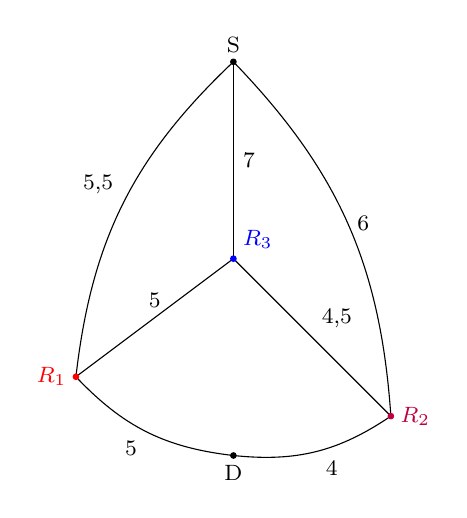
\begin{tikzpicture}[scale=1, font=\footnotesize, line join=round, line cap=round, >=stealth]
			% Các điểm
			\coordinate (D) at (0,0);
			\coordinate (R1) at (-2,1);
			\coordinate (R2) at (2,0.5);
			\coordinate (R3) at (0,2.5);
			\coordinate (S) at (0,5);
			
			% Các đường đi
			\draw (D) to[bend left=20] node[midway, below left] {5} (R1);
			\draw (D) to[bend right=20] node[midway, below right] {4} (R2);
			\draw (R1) to[bend left=20] node[midway, above left] {5,5} (S);
			\draw (R2) to[bend right=20] node[midway, right] {6} (S);
			\draw (R3) to node[midway, right] {7} (S);
			\draw (R1) to node[midway, above] {5} (R3);
			\draw (R2) to node[midway, above right] {4{,}5} (R3);
			
			% Các điểm đánh dấu
			\filldraw[black] (D) circle (1pt) node[below] {D};
			\filldraw[red] (R1) circle (1pt) node[left] {$R_1$};
			\filldraw[purple] (R2) circle (1pt) node[right] {$R_2$};
			\filldraw[blue] (R3) circle (1pt) node[above right] {$R_3$};
			\filldraw[black] (S) circle (1pt) node[above] {S};
	\end{tikzpicture}}
	\loigiai{
		\begin{itemize}
			\item 	Gọi $A$ là biến cố \lq\lq Người này ngủ lại từ nhà trú ẩn $R_1$\rq\rq. \\ $\Rightarrow P(A)=\dfrac{1}{3}$.
			\item 	Gọi $B$ là biến cố \lq\lq Người này ngủ lại từ nhà trú ẩn $R_2$\rq\rq.\\ $\Rightarrow P(B)=\dfrac{2}{3}$.
			\item 	Gọi $C$ là biến cố \lq\lq Người này ở nhà trú ẩn $R_1$ đến $R_3$\rq\rq.\\ $\Rightarrow P(C)=\dfrac{1}{4}$.
			\item 	Gọi $D$ là biến cố \lq\lq Người này ở nhà trú ẩn $R_2$ đến $R_3$\rq\rq.\\ $\Rightarrow P(D)=\dfrac{1}{3}$.
			\item Gọi $K$ là biến cố \lq\lq Người này lên đỉnh núi có tổng quảng đường lớn hơn $15$
			km\rq\rq.
		\end{itemize}
	Để tổng quãng đường lên đỉnh núi lớn hơn $15$ thì người này phải ngủ lại nhà trú ẩn $R_3$.\\
	Do đó người nay đi từ $D$ đến $R_1$ rồi qua $R_3$ và cuối cùng lên đỉnh $S$ \textbf{hoặc} người này đi từ $D$ đến $R_2$ qua $R_3$ và cuối cùng lên đỉnh $S$.\\
	Suy ra $K=AC \cup BD$.\\
	Vì $K=AC \cup BD$ nên 
	\[P(K)=P(A)\cdot P(C)+P(B)\cdot P(K)=\dfrac{1}{3}\cdot\dfrac{1}{4}+\dfrac{2}{3}\cdot\dfrac{1}{3}=\dfrac{11}{36}.\]
	}
\end{ex}

% #162 | Archive/SP_SauLuoi_2024-2025/Sp_GHKII/data/GHKII/1-TN-DS-TLN-TL-THPT-HoaHoi-BRVT-GHKII-NH24-25.tex | mã gốc 1D9H2-3
\begin{ex}%[1D9H2-3]%[Dự án tex đề GHKII THPT Hoà Hội - Bà Rịa Vũng Tàu- 24-25][Đỗ Minh Vũ]
	 			Một nhóm học sinh có $9$ học sinh nam và $12$ học sinh nữ. Chọn ngẫu nhiên $5$ học sinh từ nhóm học sinh đó. Tính xác suất của biến cố \lq\lq Có $5$ học sinh được chọn đều cùng giới tính\rq\rq.
	 		\loigiai{
	 			Gọi $A$ là biến cố \lq\lq$5$ học sinh được chọn đều là nam\rq\rq $\Rightarrow \mathrm{P}(A)=\dfrac{\mathrm{C}_9^5}{\mathrm{C}_{21} ^5}=\dfrac{2}{323}$;\\
	 			$B$ là biến cố \lq\lq$5$ học sinh được chọn đều là nữ\rq\rq $\Rightarrow \mathrm{P}(B)=\dfrac{\mathrm{C}_{12}^5}{\mathrm{C}_{21}^5}=\dfrac{88}{2261}$;\\
	 			Gọi $X$ là biến cố \lq\lq$5$ học sinh được chọn đều cùng giới tính\rq\rq, ta có $A,B$ là hai biến cố xung khắc nên 
	 			$$\Rightarrow \mathrm{P}(X) = \mathrm{P}(A\cup B) = \mathrm{P}(A)+\mathrm{P}(B) = \dfrac{6}{133}.$$
	 		}
	 	\end{ex}

% #186 | Archive/SP_SauLuoi_2024-2025/Sp_GHKII/data/GHKII/1-TL-TN-DS-THPT-Tran-Quang-Khai-GHKII-NH24-25.tex | mã gốc 1D9N1-3
\begin{ex}%[1D9N1-3]%[Dự án đề kiểm tra Toán 11 GHKII NH24-25- Phạm Phú]%[THPT Trần Quang Khải - BRVT]
	Lan và Tùng độc lập chơi ném bóng vào rổ. Mỗi bạn ném vào rổ của mình một quả bóng. Biết rằng xác suất ném bóng vào rổ của Lan là $\dfrac{3}{7}$ và của Tùng là $\dfrac{4}{5}$. Xác suất của biến cố "cả hai bạn cùng ném bóng vào rổ" có dạng $P(A)=\dfrac{a}{b}$. Tính giá trị của biểu thức $Q=a+2b$.
		\shortans[]{$82$}
	\loigiai{
	Gọi biến cố A: "Lan ném bóng trúng vào rổ"\\
	Gọi biến cố B: "Tùng ném bóng trúng vào rổ"\\
	Khi đó biến cố AB: "Cả hai bạn cùng ném bóng trúng vào rổ". \\
	Ta có $P(AB)=P(A)\cdot P(B)=\dfrac{3}{7}\cdot \dfrac{4}{5}=\dfrac{12}{35}$. Từ đó $a+2b=12+2\cdot 35=82$.
	}
\end{ex}

% #188 | Archive/SP_SauLuoi_2024-2025/Sp_GHKII/data/GHKII/1-TL-TN-DS-THPT-Tran-Quang-Khai-GHKII-NH24-25.tex | mã gốc 1D9N2-3
\begin{ex}%[1D9N2-3]%[Dự án đề kiểm tra Toán 11 GHKII NH24-25- Phạm Phú]%[THPT Trần Quang Khải - BRVT]
	Một hộp có $12$ viên bi có cùng kích thướt và khối lượng, trong đó có $7$ viên bi màu xanh và $5$ viên bi màu vàng. Chọn ngẫu nhiên $5$ viên bi từ hộp đó. Tính xác suất để trong $5$ viên  bi được chọn có ít nhất $2$ viên bi vàng.
	\loigiai{
	Ta có không gian mẫu là $n(\Omega)=C_{12}^5=792$.\\
	Gọi biến cố A " Trong 5 viên bi được chọn, có 5 viên bi màu xanh". Khi đó $n(A)=C_7^5=21$.\\
	Gọi biến cố B: " Trong $5$ viên bi được chọn, có $1$ viên bi màu vàng, có $4$ viên bi màu xanh". Khi đó $n(B)=C_5^1\cdot C_7^4=175$.\\
	Xét biến cố M "Trong $5$ viên bi được chọn có ít nhất $2$ viên bi màu vàng"\\
	Khi đó $\overline{M}:$ "trong $5$ viên  bi được chọn có nhiều nhất $1$ viên bi màu vàng"\\
	Ta có $n(\overline{M})=21+175=196$.
	Khi đó $P(\overline{M})=\dfrac{196}{792}=\dfrac{49}{198}$.\\ Suy ra $P(M)=1-P(\overline{M})=1-\dfrac{49}{198}=\dfrac{149}{198}$
	}
\end{ex}

% #213 | Archive/SP_SauLuoi_2024-2025/Sp_GHKII/data/GHKII/1-TN-DS-TLN-TL-THPT-HauNghia-LongAn-GHKII-NH24-25.tex | mã gốc 1D9V2-5
\begin{ex}%[1D9V2-5]%[Dự án đề kiểm tra Toán 11 GHKII NH24-25 - Đợt 9 - Huỳnh Đức Vũ]%[THPT Hậu Nghĩa - Long An]
Người dân Bình Định truyền nhau câu ca dao
\begin{center}
\lq\lq Muốn ăn bánh ít lá gai\\
Lấy chồng Bình Định sợ dài đường đi.\rq\rq
\end{center}
Muốn ăn bánh ít lá gai thì bạn phải tìm về với xứ Tuy Phước-Bình Định. Nơi đây nổi tiếng trứ danh với món bánh nghe cái tên khá lạ lẫm \lq\lq Bánh ít lá gai\rq\rq\, và hương vị làm say đắm lòng người. Trong một lô sản phẩm trưng bày bánh ít lá gai ở hội chợ ẩm thực huyện Tuy Phước gồm 40 chiếc bánh, $25$ chiếc bánh có nhiều hạt mè và $15$ chiếc bánh có ít hạt mè, một du khách chọn ngẫu nhiên $5$ chiếc bánh. Tính xác suất để du khách đó chọn được ít nhất $2$ chiếc bánh có nhiều hạt mè (biết rằng các chiếc bánh có khả năng được chọn là như nhau) (kết quả làm tròn đến hàng phần nghìn).
\loigiai{	
Lấy $5$ chiếc bánh bất kỳ. Có $ \mathrm{C}_{40}^5$ cách.\\
Lấy ít nhất 2 chiếc bánh có nhiều hạt mè. Có 
$\mathrm{C}_{25}^2\cdot\mathrm{C}_{15}^3+\mathrm{C}_{25}^3\cdot\mathrm{C}_{15}^2+\mathrm{C}_{25}^4\cdot\mathrm{C}_{15}^1+\mathrm{C}_{25}^5$ cách.\\
Xác suất để du khách đó chọn được ít nhất 2 chiếc bánh có nhiều hạt mè\\
$$\dfrac{\mathrm{C}_{25}^2\cdot\mathrm{C}_{15}^3+\mathrm{C}_{25}^3\cdot\mathrm{C}_{15}^2+\mathrm{C}_{25}^4\cdot\mathrm{C}_{15}^1+\mathrm{C}_{25}^5}{\mathrm{C}_{40}^5}\approx 0{,}944.$$}
\end{ex}

% #227 | Archive/SP_SauLuoi_2024-2025/Sp_GHKII/data/GHKII/1-TN-DS-TLN-TL-THPT-NinhBinh-BacLieu-GHKII-NH24-25.tex | mã gốc 1D9V2-4
\begin{ex}%[1D9V2-4]%[Dự án đề kiểm tra Toán 11 GHKII NH24-25-Lê Minh Thiện Anh]%[THPT Ninh Bình-Bạc Liêu]
	Một nhóm $50$ bệnh nhân có $32$ người điều trị bệnh X, có $18$ người điều trị cả bệnh X và bệnh Y, có $40$ người điều trị ít nhất một trong hai bệnh X hoặc Y. Chọn ngẫu nhiên một bệnh nhân. Xác suất để người đó điều trị bệnh Y và không điều trị bệnh X là $\dfrac{a}{b}$ ($a$, $b$ là các số tự nhiên và nguyên tố cùng nhau). Giá trị của $ab$ bằng bao nhiêu?
	
	\shortans[oly]{100}
	\loigiai{
		Gọi biến cố $A$: \lq\lq Người đó điều trị bệnh X\rq\rq. \\		
		Biến cố $B$: \lq\lq Người đó điều trị bệnh Y\rq\rq. \\		
		Biến cố $A \cup B$: \lq\lq Người đó điều trị ít nhất một trong hai bệnh X hoặc Y\rq\rq. \\		
		Biến cố $\overline{A}B$: \lq\lq Người đó điều trị bệnh Y và không điều trị bệnh X\rq\rq.\\
		Ta có $P(A \cup B) = P(A) + P(B) - P(AB)$ nên \\
		$P(B) = P(A \cup B) - P(A) + P(AB) = \dfrac{40}{50} - \dfrac{32}{50} + \dfrac{18}{30} = \dfrac{13}{25}$. \\
		Ta có $B = AB \cup \overline{A} B$, suy ra $P(B) = P(AB) + P(\overline{A} B)$.\\
		$\Rightarrow P(\overline{A} B) = P(B) - P(AB) = \dfrac{13}{25} - \dfrac{18}{50} = \dfrac{4}{25}$.\\		
		Vậy $\dfrac{a}{b} = \dfrac{4}{25}$. Suy ra $ab=100$.
	}
\end{ex}

% #257 | Archive/SP_SauLuoi_2024-2025/Sp_GHKII/data/GHKII/1-TN-DS-TLN-TL-THPT-Edison-HaiPhong-GKII-NH24-25.tex | mã gốc 1D9H2-4
\begin{ex}%[1D9H2-4]%[Dự án đề kiểm tra Toán 10 GHKII NH24-25- Quan Ón]%[THPT Edison - Hải Phòng]
	Nhà trường muốn chọn một đội văn nghệ có đủ cả nam và nữ gồm $12$ em đi biểu diễn từ một nhóm học sinh gồm $10$ nam sinh và $8$ nữ sinh. Xác xuất để đội văn nghệ được chọn có đúng $6$ bạn nam là $\dfrac{a}{b}$ $(a\in \mathbb{N}, b \in \mathbb{N})$; $\dfrac{a}{b}$ là phân số tối giản. Tính $a + b$.
	\shortans{291}
	\loigiai{
		Gọi $A$ là biến cố: \lq\lq Đội văn nghệ được chọn có đúng $6$ bạn nam\rq\rq.\\
		Số cách chọn $12$ học sinh bất kỳ (có cả nam và nữ) từ $18$ học sinh là $\mathrm{C}_{18}^{12} = 18\,564$ cách.\\
		Do đó $n(\Omega) = 18\,564$.\\
		Số cách chọn $12$ học sinh trong đó có đúng $6$ bạn nam là $\mathrm{C}_{10}^{6}\cdot\mathrm{C}_{8}^{6} = 5\,880$ cách.\\
		Do đó $n(A) = 5\,880$.\\
		Xác suất để đội văn nghệ được chọn có đúng $6$ bạn nam là
		$$ \mathrm{P}(A) = \dfrac{n(A)}{n(\Omega)} = \dfrac{5\,880}{18\,564} = \dfrac{70}{221}. $$
		Suy ra $a = 70$ và $b = 221 \Rightarrow a + b = 70 + 221 = 291$.
	}
\end{ex}

% #261 | Archive/SP_SauLuoi_2024-2025/Sp_GHKII/data/GHKII/1-TN-DS-TLN-TL-THPT-Edison-HaiPhong-GKII-NH24-25.tex | mã gốc 1D9H1-3
\begin{ex}%[1D9H1-3]%[Dự án đề kiểm tra Toán 10 GHKII NH24-25- Quan Ón]%[THPT Edison - Hải Phòng]
	Ba người xạ thủ $A_1$, $A_2$, $A_3$ độc lập với nhau cùng nổ súng bắn vào mục tiêu. Biết rằng xác suất bắn trúng mục tiêu của $A_1$, $A_2$, $A_3$ tương ứng là $0{,}7$, $0{,}6$ và $0{,}5$. Tính xác suất để có ít nhất một xạ thủ bắn trúng.
	\loigiai{
		Gọi 
		\begin{itemize}
			\item $A$ là biến cố: \lq\lq Xạ thủ $A_1$ bắn trúng mục tiêu\rq\rq;
			\item $B$ là biến cố: \lq\lq Xạ thủ $A_2$ bắn trúng mục tiêu\rq\rq;
			\item $C$ là biến cố: \lq\lq Xạ thủ $A_3$ bắn trúng mục tiêu\rq\rq.
		\end{itemize}
		Khi đó $A$, $B$, $C$ độc lập và $\mathrm{P}(A) = 0{,}7$; $\mathrm{P}(B) = 0{,}6$; $\mathrm{P}(C) = 0{,}5$.\\
		Xác suất cả ba xạ thủ $A_1$, $A_2$, $A_3$ đều không bắn trúng mục tiêu là 
		$$\mathrm{P}\left(\overline{A}\cdot \overline{B}\cdot \overline{C}\right) = \mathrm{P}\left(\overline{A}\right)\cdot \mathrm{P}\left(\overline{B}\right)\cdot \mathrm{P}\left(\overline{C}\right) = (1 - 0{,}7)\cdot (1 - 0{,}6)\cdot (1 - 0{,}5) = 0{,}06. $$
		Suy ra, xác suất để có ít nhất một xạ thủ bắn trúng mục tiêu là
		$$ 1 - \mathrm{P}\left(\overline{A}\cdot \overline{B}\cdot \overline{C}\right) = 1 - 0{,}06 = 0{,}94. $$
	}
\end{ex}

% #300 | Archive/2024/TOAN_10_XE/TOAN_10_XE/data4/10D8/DS10-C8-B23.tex | mã gốc 1D2B1-3
\begin{vd}%[1D2B1-3]
	Một người có $7$ cái áo trong đó có $3$ áo trắng và $5$ cái cà vạt trong đó có $2$ cà vạt màu vàng. Tìm số cách chọn một áo và một cà vạt sao chọn đã chọn áo trắng thì không chọn cà vạt màu vàng.
	\loigiai{
		\begin{enumerate}[\bfseries TH1.]
			\item Chọn $1$ áo trắng và $1$ cà vạt không phải màu vàng có $3 \times 3 = 9$ cách chọn.
			\item Chọn $1$ áo không phải áo trắng và $1$ cà vạt bất kì có $4 \times 5 = 20$ cách chọn.
		\end{enumerate}
		Theo quy tắc cộng có $9 + 20 = 29$ cách chọn.
	}
\end{vd}

% #301 | Archive/2024/TOAN_10_XE/TOAN_10_XE/data4/10D8/DS10-C8-B23.tex | mã gốc 1D2B1-3
\begin{vd}%[1D2B1-3]
	Tô màu các cạnh của hình vuông $ABCD$ bởi $6$ màu khác nhau sao cho mỗi cạnh được tô bởi một màu và hai cạnh kề nhau thì tô bởi hai màu khác nhau. Hỏi có tất cả bao nhiêu cách tô?
	\loigiai{
		Có hai trường hợp sau:
		\begin{enumerate}[TH 1.]
			\item  Nếu hai cạnh $AB$, $CD$ được tô bởi hai màu giống nhau và có số cách tô hai cạnh đó là $6$. Khi đó số cách tô hai cạnh $AD$, $BC$ là $5$ và $5$. Do đó số cách tô trong trường hợp này là $6\times 5 \times 5 = 150$.
			\item  Nếu hai cạnh $AB, CD$ được tô bởi hai màu khác nhau và có số cách tô hai cạnh đó là $6$ và $5$. Khi đó số cách tô hai cạnh $AD$, $BC$ là $4$ và $4$. Do đó số cách tô trong trường hợp này là $6\times 5 \times 4 \times 4 = 480$.
		\end{enumerate}
		Vậy số cách tô cần tìm là $150+480=630$.
	}
\end{vd}

% #302 | Archive/2024/TOAN_10_XE/TOAN_10_XE/data4/10D8/DS10-C8-B23.tex | mã gốc 1D2K1-3
\begin{vd}%[1D2K1-3]
	Một lớp học có $3$ tổ. Tổ I gồm có $3$ học sinh nam và $7$ học sinh nữ; tổ II gồm có $5$ học sinh nam và $5$ học sinh nữ; tổ III gồm có $6$ học sinh nam và $4$ học sinh nữ. Cô giáo chủ nhiệm cần chọn ra một học sinh nam và một học sinh nữ để tham gia hoạt động tình nguyện. Hỏi cô giáo có bao nhiêu cách chọn, nếu cô muốn chọn hai em học sinh ở hai tổ khác nhau?
	\loigiai{
		Ta xét các trường hợp sau:
		\begin{enumerate}[\bfseries TH1.]
			\item Chọn nam tổ 1 và nữ ở hai tổ còn lại, có $3\times 9=27$ cách.
			\item Chọn nam tổ 2 và nữ ở hai tổ còn lại, có $5\times 11=55$ cách.
			\item Chọn nam tổ 3 và nữ ở hai tổ còn lại, có $6\times 12=72$ cách.
		\end{enumerate}
		Vậy tổng số cách chọn của cô giáo là $27+55+72=154$ cách.
	}
\end{vd}

% #303 | Archive/2024/TOAN_10_XE/TOAN_10_XE/data4/10D8/DS10-C8-OTC.tex | mã gốc 1D2B1-3
\begin{ex}%[1D2B1-3]
	Có bao nhiêu số tự nhiên bé hơn $10000$ được tạo ra từ các chữ số $0$; $1$; $2$; $3$; $4$?
	\loigiai{
		Mỗi cách chọn ra một số tự nhiên bé hơn $10000$ được thực hiện theo một trong các phương án sau
		\begin{itemize}
			\item Phương án $1$. Số tạo thành có $1$ chữ số. Có $5$ cách.
			\item Phương án $2$. Số tạo thành có $2$ chữ số. Có $4\times 5=20$ cách.
			\item Phương án $3$. Số tạo thành có $3$ chữ số. Có $4\times 5 \times 5=100$ cách.
			\item Phương án $4$. Số tạo thành có $4$ chữ số. Có $4\times 5 \times 5 \times 5=500$ cách.
		\end{itemize}
		Theo quy tắc cộng, ta có số các số thỏa mãn đề bài là  $5+20+100+500=625$ số.}
\end{ex}

% #304 | Archive/2024/TOAN_10_XE/TOAN_10_XE/data4/10D8/DS10-C8-B25.tex | mã gốc 1D2Y3-1
\begin{vd}%[1D2Y3-1]
	Khai triển $\left(a+b\right)^4$
	\loigiai{
	\begin{eqnarray*}
	\left(a+b\right)^4&=&\mathrm{C}_4^0a^4+\mathrm{C}_4^1{a}^{3}b+\mathrm{C}_4^2{a}^{2}b^2+\mathrm{C}_4^3{a}^{1}b^3+\mathrm{C}_4^4b^4 \\  
		&=&a^4 +4a^3 b +6a^2 b^2 +4ab^3 +b^4.
	\end{eqnarray*}		

}
\end{vd}

% #305 | Archive/2024/TOAN_10_XE/TOAN_10_XE/data4/10D8/DS10-C8-B25.tex | mã gốc 1D2Y3-1
\begin{vd}%[1D2Y3-1]
	Khai triển $\left(a+b\right)^5$
	\loigiai{
		\begin{eqnarray*}
			\left(a+b\right)^5&=&\mathrm{C}_5^0a^5+\mathrm{C}_5^1{a}^{4}b+\mathrm{C}_5^2{a}^{3}b^2+\mathrm{C}_5^3{a}^{2}b^3+\mathrm{C}_5^4{a}^{1}b^4+\mathrm{C}_5^5b^5 \\   
			&=&a^5 +5a^4 b +10a^3 b^2 +10a^2b^3+5ab^4 +b^5.
		\end{eqnarray*}		
	}
\end{vd}

% #306 | Archive/2024/TOAN_10_XE/TOAN_10_XE/data4/10D8/DS10-C8-B25.tex | mã gốc 1D2Y3-1
\begin{vd}%[1D2Y3-1]
	Khai triển $(2x+1)^4$.
	\loigiai{
	Thay $a=2x$, $b=1$ và $n=4$ trong công thức khai triển của (1) ta được
	\begin{eqnarray*}
	\left(2x+1\right)^4&=&(2x)^4+4\cdot(2x)^{3}\cdot 1+6\cdot(2x)^{2}\cdot 1^2+4\cdot(2x)^{1}\cdot 1^3+1^4 \\ 
	&=&16x^4 +32x^3 +24x^2 +8x +1.
\end{eqnarray*}	
}
\end{vd}

% #307 | Archive/2024/TOAN_10_XE/TOAN_10_XE/data4/10D8/DS10-C8-B25.tex | mã gốc 1D2Y3-1
\begin{vd}%[1D2Y3-1]
	Khai triển $(x-2)^4$.
	\loigiai{
		Thay $a=x$, $b=-2$ và $n=4$ trong công thức khai triển của (1) ta được
	\begin{eqnarray*}
		\left(x-2\right)^4&=&x^4+4\cdot x^{3}\cdot (-2)^1+6\cdot x^{2}\cdot (-2)^2+4\cdot x^{1}\cdot (-2)^3+(-2)^4 \\ 
	&=&x^4 -8x^3 +24x^2 -32x +16.
\end{eqnarray*}		
}
\end{vd}

% #308 | Archive/2024/TOAN_10_XE/TOAN_10_XE/data4/10D8/DS10-C8-B25.tex | mã gốc 1D2Y3-1
\begin{vd}%[1D2Y3-1]
	Khai triển $(x+3)^5$.
	\loigiai{
		Thay $a=x$, $b=3$ và $n=5$ trong công thức khai triển của (1) ta được
		\begin{eqnarray*}
		\left(x+3\right)^5&=&x^5+5\cdot x^{4}\cdot 3+10\cdot x^{3}\cdot 3^2+10\cdot x^{2}\cdot 3^3+5\cdot x\cdot 3^4+3^5 \\ 
		&=&x^5+15x^4+90x^3+270x^2+405x+243.
	\end{eqnarray*}		
	}
\end{vd}

% #309 | Archive/2024/TOAN_10_XE/TOAN_10_XE/data4/10D8/DS10-C8-B25.tex | mã gốc 1D2Y3-1
\begin{vd}%[1D2Y3-1]
	Khai triển $(3x-2)^5$.
	\loigiai{
		Thay $a=3x$, $b=-2$ và $n=5$ trong công thức khai triển của (1) ta được
		\begin{eqnarray*}
		\left(3x-2\right)^5 &=&(3x)^5+5\cdot (3x)^{4}\cdot (-2)+10\cdot (3x)^{3}\cdot (-2)^2+10\cdot (3x)^{2}\cdot (-2)^3\\
		&&\quad \quad \quad \quad \quad +5\cdot (3x)\cdot (-2)^4+(-2)^5 \\ 
		&=&243x^5-810x^4+1080x^3-720x^2+240x+32.
	\end{eqnarray*}		
	}
\end{vd}

% #310 | Archive/2024/TOAN_10_XE/TOAN_10_XE/data4/10D8/DS10-C8-B25.tex | mã gốc 1D2Y3-1
\begin{vd} %[1D2Y3-1]
	Khai triển các biểu thức sau
	\begin{listEX}[2]
	\item $(x-2y)^4$;
	\item $(3x-y)^5$.
	\end{listEX}
\loigiai{
	\begin{enumerate}[a)]
		\item Ta có 
		\begin{eqnarray*}
		\left(x-2y\right)^4&=&\left[x+(-2y)\right]^4\\
		&=&x^4+4x^3(-2y)+6x^2(-2y)^2+4x(-2y)^3+(-2y)^4\\
		&=&x^4-8x^3y+24x^2y^2-32xy^3+16y^4.
		\end{eqnarray*}	
		\item Ta có 
		\begin{eqnarray*}
		\left(3x-y\right)^5&=&\left[3x+(-y)\right]^5\\
			&=&(3x)^5+5(3x)^4(-y)+10(3x)^3(-y)^2+10(3x)^2(-y)^3+5(3x)(-y)^4+(-y)^5\\
			&=&243x^5-405x^4y^3+270x^3y^2-90x^2y^3+15xy^4-y^5.
		\end{eqnarray*}	
		\end{enumerate}
}
\end{vd}

% #311 | Archive/2024/TOAN_10_XE/TOAN_10_XE/data4/10D8/DS10-C8-B25.tex | mã gốc 1D2B3-2
\begin{vd}%[1D2B3-2]
	Tìm số hạng chứa $x^{15}$ trong khai triển $\left(3x^2-2x\right)^{10}$.
	\loigiai{Theo công thức ở trên, ta có số hạng tổng quát trong khai triển là $$T_{k+1}=\mathrm{C}_{10}^k(3x^2)^{10-k}(-2x)^k=\mathrm{C}_{10}^k3^{10-k}(-2)^kx^{20-k}$$
		Số hạng chứa $x^{15}$ tương ứng với số hạng tổng quát có $k$ thỏa mãn $20-k=15\Leftrightarrow k=5$.\\
		Vậy số hạng chứa $x^{15}$ trong khai triển là $T_6=\mathrm{C}_{10}^53^{5}(-2)^5x^{15}=-6^5\mathrm{C}_{10}^5x^{15}$
	}
\end{vd}

% #312 | Archive/2024/TOAN_10_XE/TOAN_10_XE/data4/10D8/DS10-C8-B25.tex | mã gốc 1D2B3-2
\begin{vd}%[1D2B3-2]
	Tìm số hạng chứa $x^{13}$ trong khai triển $\left(x^3+2xy\right)^{21}$.
	\loigiai{Số hạng tổng quát trong khai triển $\left(x^3+2xy\right)^{21}$ là $$T_{k+1}=\mathrm{C}_{21}^k\left(x^3\right)^{21-k}\left(2xy\right)^k=2^k\mathrm{C}_{21}^kx^{63-2k}y^k$$
		Số hạng chứa $x^{13}$ tương ứng với số hạng có $k$ thỏa mãn $63-2k=13\Leftrightarrow k=25$.\\
		Vậy số hạng chứa $x^{13}$ trong khai triển đã cho là $T_{26}=2^{25}\mathrm{C}_{12}^{25}x^{13}y^{25}.$
	}
\end{vd}

% #313 | Archive/2024/TOAN_10_XE/TOAN_10_XE/data4/10D8/DS10-C8-B25.tex | mã gốc 1D2B3-2
\begin{vd}%[1D2B3-2]
	Tìm hệ số của $x^{12}$ trong khai triển $\left(1+x^2\right)^n$, biết tổng tất cả các hệ số trong khai triển đó bằng $1024$.
	\loigiai{Ta có
		$$\left(1+x^2\right)^n=\sum\limits_{k=0}^n\mathrm{C}_n^k(x^2)^k$$
		Gọi $S$ là tổng tất cả các hệ số trong khai triển, khi đó $S=\sum\limits_{k=0}^n\mathrm{C}_n^k=(1+1)^2=2^n$.\\
		Do đó $2^n=1024\Rightarrow n=10$.\\
		Số hạng tổng quát trong khai triển $\left(1+x^2\right)^{10}$ là $T_{k+1}=\mathrm{C}_{10}^k(x^2)^k=\mathrm{C}_{10}^kx^{2k}$.\\
		Số hạng chứa $x^{12}$ tương ứng với số hạng tổng quát có $k$ thỏa mãn $2k=12\Leftrightarrow k=6$.\\
		Vậy hệ số của $x^{12}$ trong khai triển là $\mathrm{C}_{10}^6=210$.
	}
\end{vd}

% #314 | Archive/2024/TOAN_10_XE/TOAN_10_XE/data4/10D8/DS10-C8-B25.tex | mã gốc 1D2K3-2
\begin{vd}%[1D2K3-2]
	Cho $x>0$ và $n$ là số tự nhiên thỏa mãn điều kiện $\mathrm{C}_{n+4}^{n+1}-\mathrm{C}_{n+3}^n=7(n+3)$. Tìm số hạng chứa $x^{19}$ trong khai triển $\left(\dfrac{1}{x^3}+x^8\right)^n$.
	\loigiai{Ta có
		\begin{align*}
			\mathrm{C}_{n+4}^{n+1}-\mathrm{C}_{n+3}^n=7(n+3)& \Leftrightarrow \dfrac{(n+4)(n+3)(n+2)}{3!}- \dfrac{(n+3)(n+2)(n+1)}{3!}=7(n+3)\\
			& \Leftrightarrow (n+4)(n+2)-(n+2)(n+1)=42 \ (\text{do } n+3>0) \\
			& \Leftrightarrow 3n=36\Leftrightarrow n=12.
		\end{align*}
		Số hạng tổng quát trong khai triển $\left(\dfrac{1}{x^3}+x^8\right)^n$ với $n=12$ là $$T_{k+1}=\mathrm{C}_{12}^k\left(\dfrac{1}{x^3}\right)^{12-k}\left(x^8\right)^k=\mathrm{C}_{12}^kx^{11k-36}$$
		Số hạng chứa $x^{19}$ tương ứng với số hạng có $k$ thỏa mãn $11k-36=19\Leftrightarrow k=5$.\\
		Vậy số hạng chứa $x^{19}$ trong khai triển đã cho là $\mathrm{C}_{12}^{5}x^{19}.$
	}
\end{vd}

% #315 | Archive/2024/TOAN_10_XE/TOAN_10_XE/data4/10D8/DS10-C8-B25.tex | mã gốc 1D2B3-3
\begin{vd}%[1D2B3-3]
	Với $n$ là số nguyên dương, chứng minh rằng: $1+4\mathrm{C}_n^1+4^2\mathrm{C}_n^2+\cdots+4^n\mathrm{C}_n^n=5^n$.
	\loigiai{
		Áp dụng khai triển nhị thức ta có:\\ 
		$VT=1+4\mathrm{C}_n^1+4^2\mathrm{C}_n^2+\cdots+4^n\mathrm{C}_n^n=\mathrm{C}_n^0+4\mathrm{C}_n^1+4^2\mathrm{C}_n^2+\cdots+4^n\mathrm{C}_n^n=(1+4)^n=5^n=VP$ \\$\Rightarrow $ điều phải chứng minh.
	}
\end{vd}

% #316 | Archive/2024/TOAN_10_XE/TOAN_10_XE/data4/10D8/DS10-C8-B25.tex | mã gốc 1D2B3-3
\begin{vd}%[1D2B3-3]
	Với $n$ là số nguyên dương, chứng minh rằng:\begin{center}
		$4^n\mathrm{C}_n^0-4^{n-1}\mathrm{C}_n^1+4^{n-2}\mathrm{C}_n^2+\cdots+(-1)^n\mathrm{C}_n^n=\mathrm{C}_n^0+2\mathrm{C}_n^1+2^2\mathrm{C}_n^2+\cdots+2^n\mathrm{C}_n^n$.
	\end{center}
	\loigiai{
		Trong khai triển nhị thức Newton:\\
		$\circ$ Chọn $a=4,b=-1\Rightarrow $ $4^n\mathrm{C}_n^0-4^{n-1}\mathrm{C}_n^1+4^{n-2}\mathrm{C}_n^2+\cdots+(-1)^n\mathrm{C}_n^n=3^n$.\\
		$\circ$ Chọn $a=1,b=2\Rightarrow $ $\mathrm{C}_n^0+2\mathrm{C}_n^1+2^2\mathrm{C}_n^2+\cdots+2^n\mathrm{C}_n^n=3^n$.\\
		Từ đó ta có điều phải chứng minh.
	}
\end{vd}

% #317 | Archive/2024/TOAN_10_XE/TOAN_10_XE/data4/10D8/DS10-C8-B25.tex | mã gốc 1D2B3-3
\begin{vd}%[1D2B3-3]
	Tính tổng $S=2^{18}\mathrm{C}_{18}^0-2^{17}\mathrm{C}_{18}^1+2^{16}\mathrm{C}_{18}^2-\cdots+\mathrm{C}_{18}^{18}$.
	\loigiai{
		Các số hạng của tổng đều có dạng: $\mathrm{C}_{18}^k 2^{18-k}(-1)^k$.\\ Do đó: 
		$S=2^{18}\mathrm{C}_{18}^0-2^{17}\mathrm{C}_{18}^1+2^{16}\mathrm{C}_{18}^2-\cdots+\mathrm{C}_{18}^{18}=\displaystyle\sum\limits_{k=0}^{18}{\mathrm{C}_{18}^k 2^{18-k}(-1)^k}=(2-1)^{18}=1$.
	}
\end{vd}

% #318 | Archive/2024/TOAN_10_XE/TOAN_10_XE/data4/10D8/DS10-C8-B24.tex | mã gốc 1D2Y2-1
\begin{vd}%[1D2Y2-1]
	Số cách xếp thứ tự đá luân lưu 11m của $5$ cầu thủ là bao nhiêu?
	\loigiai{Số cách sắp xếp là $5!=120$ cách.} 
\end{vd}

% #319 | Archive/2024/TOAN_10_XE/TOAN_10_XE/data4/10D8/DS10-C8-B24.tex | mã gốc 1D2Y2-1
\begin{vd}%[1D2Y2-1]
	Trong một cuộc thi điền kinh gồm $6$ vận động viên chạy trên $6$ đường chạy. Hỏi có bao nhiêu cách xếp các vận động viên vào các đường chạy đó?
	\loigiai{Số cách sắp xếp là $6!=720$ cách.} 
\end{vd}

% #320 | Archive/2024/TOAN_10_XE/TOAN_10_XE/data4/10D8/DS10-C8-B24.tex | mã gốc 1D2Y2-1
\begin{vd}%[1D2Y2-1]
	Ở các căn hộ chung cư, người ta thường dùng các chữ số để tạo mật mã mở cửa. Gia đình bạn Linh đặt mật mã nhà là một dãy gồm $6$ chữ số đôi một khác nhau. Hỏi gia đình bạn Linh có bao nhiêu cách để tạo mật mã.
	\loigiai{Mỗi mật mã của gia đình bạn Linh là một chỉnh hợp chập $6$ của $10$ chữ số.\\
	Vậy có $\mathrm{A}_{10}^6=151200$ cách chọn.}
\end{vd}

% #321 | Archive/2024/TOAN_10_XE/TOAN_10_XE/data4/10D8/DS10-C8-B24.tex | mã gốc 1D2Y2-1
\begin{vd}%[1D2Y2-1]
Trong một giải đua ngựa gồm $12$ con ngựa, người ta chỉ quan tâm đến $3$ con ngựa: con nhanh nhất, nhanh nhì và nhanh thứ ba. Hỏi có bao nhiêu kết quả có thể xảy ra?
	\loigiai{Số kết quả có thể xảy ra là $\mathrm{A}_{12}^3=1320$ kết quả.} 
\end{vd}

% #322 | Archive/2024/TOAN_10_XE/TOAN_10_XE/data4/10D8/DS10-C8-B24.tex | mã gốc 1D2Y2-1
\begin{vd}%[1D2Y2-1]
	Từ các chữ số $1$, $2$, $3$, $4$, $5$, $6$, $7$, $8$, ta lập được bao nhiêu số tự nhiên
	\begin{enumerate}
		\item Gồm $8$ chữ số đôi một khác nhau?
		\item Gồm $6$ chữ số đôi một khác nhau?
	\end{enumerate}
\loigiai{
\begin{enumerate}
	\item Số số tự nhiên có $8$ chữ số đôi một khác nhau có thể được lập là $8!=40320$ cách.
	\item Số số tự nhiên có $6$ chữ số đôi một khác nhau có thể được lập là $\mathrm{A}_8^6=20160$ cách.
\end{enumerate}}
\end{vd}

% #323 | Archive/2024/TOAN_10_XE/TOAN_10_XE/data4/10D8/DS10-C8-B24.tex | mã gốc 1D2Y2-1
\begin{vd}%[1D2Y2-1]
Có $7$ bạn học sinh muốn chơi cờ cá ngựa, nhưng mỗi ván chỉ có $4$ người chơi. Hỏi có bao nhiêu cách chọn $4$ bạn chơi cờ cá ngựa?
	\loigiai{Số cách chọn $4$ bạn chơi cờ cá ngựa là $\mathrm{C}_7^4=35$ cách.} 
\end{vd}

% #324 | Archive/2024/TOAN_10_XE/TOAN_10_XE/data4/10D8/DS10-C8-B24.tex | mã gốc 1D2B2-2
\begin{vd}%[Tex hóa BTN1]%[Nhật Thiện - pb Pham Anh]%[1D2B2-2]
	Một câu lạc bộ có $20$ học sinh.
	\begin{enumerate}
		\item Có bao nhiêu cách chọn $6$ thành viên vào Ban quản lí?
		\item Có bao nhiêu cách chọn $1$ Trưởng ban, $1$ Phó ban, $4$ thành viên khác vào Ban quản lí?
	\end{enumerate}
\loigiai{
\begin{enumerate}
	\item Chọn $6$ học sinh vào Ban quản lí có $\mathrm{C}_{20}^6$ cách.
	\item Chọn $1$ Trưởng ban, $1$ Phó ban vào Ban quản lí có $\mathrm{A}_{20}^6$ cách.\\
	Chọn $4$ thành viên khác vào Ban quản lí có $\mathrm{C}_{18}^4$ cách.\\
	Vậy có $\mathrm{A}_{20}^6\cdot \mathrm{C}_{18}^4$ cách chọn.
\end{enumerate}
}
\end{vd}

% #325 | Archive/2024/TOAN_10_XE/TOAN_10_XE/data4/10D8/DS10-C8-B24.tex | mã gốc 1D2B2-2
\begin{vd}%[Tex hóa BTN1]%[Nhật Thiện - pb Pham Anh]%[1D2B2-2]
	Có bao nhiêu số tự nhiên có năm chữ số khác nhau tạo ra từ các chữ số $1, 2, 3, 4, 5, 6, 7, 8$ trong đó bắt buộc phải có $3$ chữ số chẵn và $2$ chữ số lẻ?
	\loigiai{
		Gọi số tạo thành là $\overline{abcde}$ \quad(các chữ số $a$, $b$, $c$, $d$ đôi một khác nhau).\\
		Lấy $3$ chữ số chẵn trong các chữ số $2, 4, 6, 8$ có $\mathrm{C}_4^3$ cách.\\
		Lấy $2$ chữ số lẻ trong các chữ số $1, 3, 5, 7$ có $\mathrm{C}_4^2$ cách.\\
		Hoán vị $5$ chữ số vừa lấy ($3$ chẵn, $2$ lẻ) vào $5$ vị trí $a,b,c,d,e$ có $5!$ cách.\\
		Theo quy tắc nhân có $\mathrm{C}_4^3\cdot\mathrm{C}_4^2\cdot 5!=2880$ số cần tìm.
	}
\end{vd}

% #326 | Archive/2024/TOAN_10_XE/TOAN_10_XE/data4/10D8/DS10-C8-B24.tex | mã gốc 1D2B2-2
\begin{vd}%[Tex hóa BTN1]%[Nhật Thiện - pb Pham Anh]%[1D2B2-2]
	Một bàn dài có $6$ ghế được đánh số từ $1$ đến $6$. Cô Trinh muốn xếp $3$ bạn nam và $3$ bạn nữ ngồi vào bàn với điều kiện ghế số $1$ và ghế số $2$ phải là $2$ bạn nữ. Hỏi cô Trinh có bao nhiêu cách xếp như vậy?
	\loigiai{
		Số cách thỏa mãn yêu cầu bài toán được mô tả như sau:
		\begin{itemize}
			\item Chọn $2$ nữ trong $3$ nữ sắp xếp vào ghế số $1$ và ghế số $2$ nên có $\mathrm{A}_3^2$ cách.
			\item Sắp xếp $4$ bạn gồm $3$ bạn nam và $1$ bạn nữ còn lại vào $4$ ghế trống có $4!$ cách.
		\end{itemize}
		Do đó số cách sắp xếp là $\mathrm{A}_3^2\cdot 4!=144$ (cách).
	}	
\end{vd}

% #327 | Archive/2024/TOAN_10_XE/TOAN_10_XE/data4/10D8/DS10-C8-B24.tex | mã gốc 1D2K2-2
\begin{vd}%[Tex hóa BTN1]%[Nhật Thiện - pb Pham Anh]%[1D2K2-2]
	Có bao nhiêu cách sắp xếp $5$ người gồm $3$ nam và $2$ nữ vào một hàng ghế gồm $7$ ghế để $3$ nam ngồi kề nhau, $2$ nữ ngồi kề nhau?
	\loigiai{
		Xét $3$ loại ghế gồm $1$ ghế $3$ chỗ ngồi, $1$ ghế $2$ chỗ ngồi và $2$ ghế $1$ chỗ ngồi.\\
		Chọn $2$ trong $4$ vị trí để xếp loại ghế $2$ và $3$ chỗ ngồi có $\mathrm{A}_4^2$ cách.\\
		Xếp $3$ nam vào loại ghế $3$ chỗ ngồi có $3!$ cách.\\
		Xếp $2$ nữ vào loại ghế $2$	chỗ ngồi có $2!$ cách.\\
		Theo quy tắc nhân có $\mathrm{A}_4^2\cdot 3!\cdot 2!=144$ cách xếp.
	}
\end{vd}

% #328 | Archive/2024/TOAN_10_XE/TOAN_10_XE/data4/10D8/DS10-C8-B24.tex | mã gốc 1D2B2-5
\begin{vd}%[Phạm Tuấn]%[1D2B2-5] 
Có bao nhiêu số tự nhiên gồm $6$ chữ số sao cho trong mỗi số có đúng $2$ chữ số $1$, $3$ chữ số $2$  và $1$ chữ số $3$ (ví dụ $123221$, $112322$)?
\loigiai{
Ta thấy mỗi số cần tìm là hoán vị lặp của $2$ chữ số $1$, $3$ chữ số $2$  và $1$ chữ số $3$. \\
Vậy có  tất  cả $\dfrac{6!}{2! \cdot 3!} = 60$  số tự nhiên.
}
\end{vd}

% #329 | Archive/2024/TOAN_10_XE/TOAN_10_XE/data4/10D8/DS10-C8-B24.tex | mã gốc 1D2B2-5
\begin{vd}%[Phạm Tuấn]%[1D2B2-5] 
Có bao nhiêu cách sắp xếp $3$ quả cầu xanh giống nhau, $4$ quả cầu đỏ giống nhau và $5$ quả cầu vàng giống nhau theo một hàng ngang?
\loigiai{
Áp dụng công thức hoán vị lặp, ta có số cách sắp xếp là   $\dfrac{12!}{3! \cdot 4! \cdot 5!} = 27720$.
}
\end{vd}

% #330 | Archive/2024/TOAN_10_XE/TOAN_10_XE/data4/10D8/DS10-C8-B24.tex | mã gốc 1D2B2-5
\begin{vd}%[Phạm Tuấn]%[1D2B2-5] 
Từ các chữ số $2$ và $3$ lập được bao nhiêu số tự nhiên có $5$ chữ số sao cho tổng các chữ số bằng $12$?
\loigiai{
Gọi $a$ và $b$ lần lượt là số chữ số $2$ và số chữ số $3$. \\
Ta có $\heva{&a+b=5\\&2a+3b=12} \Leftrightarrow \heva{&a=3\\&b=2.}$   \\
Ta thấy mỗi số cần tìm là hoán vị lặp của $3$ chữ số $2$ và $2$ chữ số $3$. \\
Vậy có  tất  cả $\dfrac{5!}{2! \cdot 3!} = 10$  số tự nhiên.
}
\end{vd}

% #331 | Archive/2024/TOAN_10_XE/TOAN_10_XE/data4/10D8/DS10-C8-B24.tex | mã gốc 1D2B2-5
\begin{vd}%[Phạm Tuấn]%[1D2B2-5] 
Một xâu nhị phân độ dài $n$ là một dãy liên tiếp $n$ các chữ số $0$  và $1$ (ví dụ $011$, $101$, $000$ là các xâu độ dài $3$). Có tất cả bao nhiêu xâu nhị phân độ dài $11$ bao gồm  $3$  chữ số $0$  và  $8$ chữ số $1$?
\loigiai{
Mỗi xâu nhị phân cần tìm là một hoán vị lặp của $3$  chữ số $0$  và  $8$ chữ số $1$. \\
Vậy có  tất  cả $\dfrac{11!}{3! \cdot 8!} = 165$  xâu nhị phân.
}
\end{vd}

% #332 | Archive/2024/TOAN_10_XE/TOAN_10_XE/data4/10D8/DS10-C8-B24.tex | mã gốc 1D2K2-5
\begin{vd}%[Phạm Tuấn]%[1D2K2-5] 
Có tất cả bao nhiêu số tự nhiên có $9$ chữ số sao cho mỗi số tự nhiên có $3$ chữ số $0$, $3$ chữ số $3$, $2$ chữ số $5$  và $1$ chữ số $8$?
\loigiai{
Số hoán vị lặp của $3$ chữ số $0$, $3$ chữ số $3$, $2$ chữ số $5$  và $1$ chữ số $8$ là  $\dfrac{9!}{3! \cdot 3! \cdot 2!}$. \\
Nếu chữ số $0$ đứng đầu thì số hoán vị lặp của $2$ chữ số $0$, $3$ chữ số $3$, $2$ chữ số $5$  và $1$ chữ số $8$ là $\dfrac{8!}{2! \cdot 3! \cdot 2!}$. \\
Vậy có  tất  cả $\dfrac{9!}{3! \cdot 3! \cdot 2!} - \dfrac{8!}{2! \cdot 3! \cdot 2!} = 3360$ số tự nhiên.
}
\end{vd}

% #333 | Archive/2024/TOAN_10_XE/TOAN_10_XE/data4/10D8/DS10-C8-B24.tex | mã gốc 1D2K2-5
\begin{vd}%[Phạm Tuấn]%[1D2K2-5]
Cho phương trình $x_1+x_2+x_3+x_4+x_5 =8$ $(*)$. Mỗi nghiệm $(x_1;x_2;x_3;x_4;x_5)$ của phương trình $(*)$ được gọi là một nghiệm nguyên dương  nếu $x_1,x_2,x_3,x_4,x_5$  là các số nguyên dương. Phương trình $(*)$ có tất cả bao nhiêu nghiệm nguyên dương thỏa mãn $x_k \leq 4$ với $k=1,2,3,4,5$?
\loigiai{
Ta xét các phân tích của $8$ thành tổng của các chữ số $1,2,3,4$.
\begin{align*}
8&=1+1+1+1+4  & (1)\\
&=1+1+1+2+3 & (2)\\
&=1+1+2+2+2. & (3)
\end{align*}
\begin{itemize}
\item Với phân tích (1), số nghiệm của $(*)$ bằng số hoán vị lặp của $4$  chữ số $1$  và  $1$ chữ số $4$. \\
Suy ra có  $\dfrac{5!}{4!} = 5$ nghiệm.
\item Với phân tích (2), số nghiệm của $(*)$ bằng số hoán vị lặp của $3$  chữ số $1$  và  $1$ chữ số $2$, $1$ chữ số $3$. \\
Suy ra có  $\dfrac{5!}{3!} = 20$ nghiệm.
\item Với phân tích (3), số nghiệm của $(*)$ bằng số hoán vị lặp của $2$  chữ số $1$  và  $3$ chữ số $2$. \\
Suy ra có  $\dfrac{5!}{2! \cdot 3!} = 10$ nghiệm.
\end{itemize}
Vậy có tất cả $5+20+10=35$ nghiệm.
}
\end{vd}

% #334 | Archive/2024/TOAN_10_XE/TOAN_10_XE/data4/10D8/DS10-C8-B24.tex | mã gốc 1D2B2-4
\begin{vd}%[Phạm Tuấn]%[1D2B2-4]
Có bao nhiêu cách sắp xếp $10$  học sinh vào một bàn tròn?
\loigiai{
Ta thấy mỗi cách sắp xếp là một hoán vị vòng quanh của $10$ phần tử. \\
Vậy có $9!$ cách sắp xếp.
}
\end{vd}

% #335 | Archive/2024/TOAN_10_XE/TOAN_10_XE/data4/10D8/DS10-C8-B24.tex | mã gốc 1D2B2-4
\begin{vd}%[Phạm Tuấn]%[1D2B2-4] 
Có bao nhiêu cách sắp xếp $6$ học sinh nam và $6$ học sinh nữ vào một bàn tròn sao cho nam, nữ ngồi xen kẽ nhau?
\loigiai{
Có $5!$ cách sắp xếp $6$ nam. \\
Sau khi sắp xếp $6$ nam có $6!$ cách sắp xếp $6$ nữ. \\
Vậy có $5! \cdot 6! = 86400$ cách sắp xếp.
}
\end{vd}

% #336 | Archive/2024/TOAN_10_XE/TOAN_10_XE/data4/10D8/DS10-C8-B24.tex | mã gốc 1D2B2-4
\begin{vd}%[Phạm Tuấn]%[1D2B2-4]
Có bao nhiêu cách sắp xếp $5$ học sinh nam và $3$ học sinh nữ vào một bàn tròn sao cho các học sinh nam ngồi cạnh nhau, các học sinh nữ ngồi cạnh nhau? 
\loigiai{
Ta coi $5$ học sinh nam là nhóm A,  $3$ học sinh nữ là nhóm B. \\
Có $(2-1)!=1$ cách sắp xếp hai nhóm A và B. \\
Có $5!$ cách sắp xếp $5$ học sinh nam. \\
Có $3!$ cách sắp xếp $3$ học sinh nữ. \\
Vậy có $5! \cdot 3! = 720$ cách sắp xếp.
}
\end{vd}

% #337 | Archive/2024/TOAN_10_XE/TOAN_10_XE/data4/10D8/DS10-C8-B24.tex | mã gốc 1D2K2-4
\begin{vd}%[Phạm Tuấn]%[1D2K2-4]
Có $12$ quả cầu kích thước khác nhau, trong đó có $3$ quả cầu xanh, $3$ quả cầu đỏ, $5$ quả cầu vàng, $2$ quả cầu trắng.  Có bao nhiêu cách sắp xếp $12$ quả cầu theo vòng tròn sao cho các quả cầu cùng màu nằm cạnh nhau?
\loigiai{
Gọi nhóm các quả cầu cùng màu lần lượt là $X,Y,Z,T$.  \\
Có $(4-1)!=6$ cách sắp xếp các nhóm $X,Y,Z,T$ theo  vòng tròn. \\
Có $3!$ cách sắp xếp $3$ quả cầu xanh. \\
Có $3!$ cách sắp xếp $3$ quả cầu đỏ. \\
Có $5!$ cách sắp xếp $5$ quả cầu vàng. \\
Có $2!$ cách sắp xếp $2$ quả cầu trắng. \\
Vậy có $6 \cdot 3! \cdot 3! \cdot 5! \cdot 2! = 51840$ cách sắp xếp.
}
\end{vd}

% #338 | Archive/2024/TOAN_10_XE/TOAN_10_XE/data4/10D8/DS10-C8-B24.tex | mã gốc 1D2K2-4
\begin{vd}%[Phạm Tuấn]%[1D2K2-4]
Có $11$ quả cầu kích thước khác nhau, trong đó có $2$ quả cầu xanh, $3$ quả cầu đỏ, $3$ quả cầu vàng, $3$ quả cầu trắng.  Có bao nhiêu cách sắp xếp $11$ quả cầu theo vòng tròn sao cho $2$ quả cầu xanh nằm cạnh nhau và $3$ quả cầu đỏ nằm cạnh nhau?
\loigiai{
Ta coi $2$ quả cầu xanh và $3$ quả cầu đỏ là $1$ quả cầu xanh và $1$ quả cầu đỏ. \\ 
Có $(8-1)!=7!$ cách sắp xếp $8$ quả cầu theo  vòng tròn. \\
Có $2!$ cách sắp xếp $2$ quả cầu xanh. \\
Có $3!$ cách sắp xếp $3$ quả cầu đỏ. \\
Vậy có $7! \cdot 2! \cdot 3! = 60480$ cách sắp xếp.
}
\end{vd}

% #339 | Archive/2024/TOAN_10_XE/TOAN_10_XE/data4/10D8/DS10-C8-BTRL25.tex | mã gốc 1D2B3-2
\begin{bt}%[1D2B3-2]
	Tìm hệ số của số hạng chứa $x^3$ trong khai triển biểu thức $\left(x^2+\dfrac{2}{x}\right)^{21}$.
	\loigiai{Số hạng tổng quát trong khai triển $\left(x^2+\dfrac{2}{x}\right)^{21}$ là $T_{k+1}=\mathrm{C}_{21}^k\cdot (x^2)^{21-k}\left(\dfrac{2}{x}\right)^k=\mathrm{C}_{21}^k2^kx^{42-3k}$.\\
		Số hạng chứa $x^3$ tương ứng với số hạng chứa $k$ thỏa mãn $42-3k=3\Leftrightarrow k=13$. Từ đó suy ra hệ số của $x^3$ trong khai triển là $2^{13}\mathrm{C}_{21}^{13}$.}
\end{bt}

% #340 | Archive/2024/TOAN_10_XE/TOAN_10_XE/data4/10D8/DS10-C8-BTRL25.tex | mã gốc 1D2B3-2
\begin{bt}%[1D2B3-2]
	Tìm hệ số của số hạng $x^{25}y^{10}$ trong khai triển $\left(x^3+xy\right)^{15}$.
	\loigiai{
		Số hạng tổng quát của khai triển là $T_{k+1}=\mathrm{C}_{15}^k(x^3)^{15-k}(xy)^k=\mathrm{C}_{15}^kx^{45-2k}y^k$.\\
		Số hạng chứa $x^{25}y^{10}$ tương ứng với $k=10$, từ đó suy ra hệ số của $x^{25}y^{10}$ là $\mathrm{C}_{15}^{10}=3003.$
	}
\end{bt}

% #341 | Archive/2024/TOAN_10_XE/TOAN_10_XE/data4/10D8/DS10-C8-BTRL25.tex | mã gốc 1D2B3-2
\begin{bt}%[1D2B3-2]
	Biết tổng các hệ số của ba số hạng đầu trong khai triển $\left(x^3+\dfrac{1}{x^2}\right)^n$ bằng 11. Tìm hệ số của $x^7$ trong khai triển đó.
	\loigiai{
		Theo đề cho $\mathrm{C}_{n}^0+\mathrm{C}_{n}^1+\mathrm{C}_{n}^2=11 \Rightarrow n=4$.\\
		Số hạng tổng quát trong khai triển $\left(x^3+\dfrac{1}{x^2}\right)^4$ là $T_{k+1}=\mathrm{C}_{4}^k(x^3)^{4-k}(x^{-2})^k=\mathrm{C}_{4}^kx^{12-5k}$.\\
		Từ đó suy ra hệ số của $x^7$ trong khai triển là $\mathrm{C}_{4}^1=4$.
	}
\end{bt}

% #342 | Archive/2024/TOAN_10_XE/TOAN_10_XE/data4/10D8/DS10-C8-BTRL25.tex | mã gốc 1D2K3-2
\begin{bt}%[1D2K3-2]
	Khai triển biểu thức $(1+x)^9+(1+x)^{10}+\cdots+(1+x)^{14}$ ta được đa thức:
	$$Q(x)=a_0+a_1x+\cdots+a_{14}x^{14}$$
	Hãy xác định $a_{10}$.
	\loigiai{Trước hết ta thấy với $k\leq n$ thì hệ số của $x^k$ trong khai triển $(1+x)^n$ là $\mathrm{C}_n^k$. Từ đó suy ra hệ số của $x^{10}$ trong các khai triển $(1+x)^9,(1+x)^{10},\ldots,(1+x)^{14}$ lần lượt là $0, \mathrm{C}_{10}^{10},\cdots,\mathrm{C}_{14}^{10}$.\\
		Từ đó suy ra $a_{10}=\mathrm{C}_{10}^{10}+\cdots+\mathrm{C}_{14}^{10}=1365$.
	}
\end{bt}

% #343 | Archive/2024/TOAN_10_XE/TOAN_10_XE/data4/10D8/DS10-C8-BTRL25.tex | mã gốc 1D2G3-2
\begin{bt}%[1D2G3-2]
	Tìm hệ số của $x^8$ trong khai triển thành đa thức của biểu thức $\left(1+ x^2-x^3\right)^8$.
	\loigiai{Ta có
		\begin{align*}
			\left(1+ x^2-x^3\right)^8&=\left[1+x^2\left(1-x\right)\right]^8\\
			&= \sum\limits_{k = 0}^8\mathrm{C}_8^k\left[x^2(1-x)\right]^k= \sum\limits_{k = 0}^8 \mathrm{C}_8^kx^{2k}(1 - x)^k\\
			&= \sum\limits_{k = 0}^8 \mathrm{C}_8^kx^{2k}\left(\sum\limits_{i = 0}^k\mathrm{C}_k^i(-x)^i\right)= \sum\limits_{k = 0}^8 \sum\limits_{i = 0}^k \mathrm{C}_8^kx^{2k}\mathrm{C}_k^i(-1)^ix^i \\
			&= \sum\limits_{k = 0}^8 \sum\limits_{i = 0}^k \mathrm{C}_8^k\mathrm{C}_k^i(-1)^ix^{2k + i}
		\end{align*}
		Số hạng chứa $x^8$ tương ứng số hạng chứa $k$ và $i$ thỏa $2k+i=8$.\\
		Vì $0\leq i\leq k\leq 8$ nên $2k + i = 8 \Leftrightarrow \heva{&k = 3\\&i = 2}$ hoặc $\heva{&k = 4\\&i = 0}$.\\
		Vậy hệ số của số hạng chứa $x^8$ là $\mathrm{C}_8^3\mathrm{C}_3^2{( - 1)^2} + \mathrm{C}_8^4\mathrm{C}_4^0{( - 1)^0} = 238$.
	}
\end{bt}

% #344 | Archive/2024/TOAN_10_XE/TOAN_10_XE/data4/10D8/DS10-C8-BTRL25.tex | mã gốc 1D2B3-2
\begin{bt}%[1D2B3-2]
	Tìm số hạng không chứa $x$ trong khai triển $P(x) = \left(2 x^2 + \dfrac{3}{x}\right)^6$ (với $x$ khác $0$). 
	\loigiai{
		Số hạng tổng quát của khai triển là $T_{k+1}=\mathrm{C}^k_{6} (2 x^2)^{6-k} \left(\dfrac{3}{x}\right)^k = \mathrm{C}^k_6 2^{6-k} 3^k x^{12-3k}$. \\
		Ta phải tìm $k$ sao cho $12 - 3k =0 \Leftrightarrow k=4$. \\
		Vậy số hạng cần tìm là $\mathrm{C}^4_{6} (2)^{6-4} 3^4 = 4860$. 
	}
\end{bt}

% #345 | Archive/2024/TOAN_10_XE/TOAN_10_XE/data4/10D8/DS10-C8-BTRL25.tex | mã gốc 1D2K3-2
\begin{bt}%[1D2K3-2]
	Tìm số hạng không chứa $x$ trong khai triển $P(x) = \left(x - \dfrac{1}{x} \right)^{n}$ (với $x$ khác $0$) biết $2 \mathrm{C}^2_n = \mathrm{C}^3_n$. 
	\loigiai{
		Điều kiện $n \geq 3$, $n \in \mathbb{N}$.\\
		Ta có $2 \mathrm{C}^2_n = \mathrm{C}^3_n \Leftrightarrow 2. \dfrac{n!}{(n-2)! 2!} = \dfrac{n!}{(n-3)! 3!} \Leftrightarrow \dfrac{2}{n-2} = \dfrac{1}{3} \Leftrightarrow n = 8$.\\
		Với $n=8$, số hạng tổng quát của khai triển là 
		$T_{k+1}=\mathrm{C}^k_{8} x^{8-k} (-1)^k  x^{-k} = \mathrm{C}^k_{8} x^{8-2k}(-1)^k$.\\
		Ta phải tìm $k$ sao cho $8 - 2k =0 \Leftrightarrow k=4$. 
		Vậy số hạng cần tìm là $\mathrm{C}^4_{8}=70$. 
	}
\end{bt}

% #346 | Archive/2024/TOAN_10_XE/TOAN_10_XE/data4/10D8/DS10-C8-BTRL25.tex | mã gốc 1D2K3-2
\begin{bt}%[1D2K3-2]
	Cho khai triển $P(x)=\left(x+\dfrac{1}{3}\right)^n$. Tìm số hạng không chứa $x$ trong khai triển, biết hệ số của số hạng thứ ba trong khai triển bằng $5$. 
	\loigiai{
		Số hạng tổng quát của khai triển là $T_{k+1}=\mathrm{C}^k_n x^{n-k} 3^{-k}$.\\
		Hệ số của số hạng thứ ba trong khai triển bằng $5$ nên $\dfrac{1}{9}\mathrm{C}^2_n=5\Leftrightarrow n=9$.\\
		Với $n=9$, số hạng tổng quát của khai triển là $\mathrm{C}^k_9 x^{9-k} 3^{-k}$.\\
		Ta tìm $k$ sao cho $9-k =0 \Leftrightarrow k=9$.\\
		Vậy số hạng không chứa $x$ là $\mathrm{C}^9_9 3^{-9}=\dfrac{1}{19683}$. 
	}
\end{bt}

% #347 | Archive/2024/TOAN_10_XE/TOAN_10_XE/data4/10D8/DS10-C8-BTRL25.tex | mã gốc 1D2K3-2
\begin{bt}%[1D2K3-2]
	Tìm số hạng không chứa $x$ trong khai triển $P(x)=\left(x+\dfrac{2}{x^2}\right)^{n}$ (với $x$ khác $0$) biết $\mathrm{C}^{6}_{n}+3\mathrm{C}^{7}_{n}+3\mathrm{C}^{8}_{n}+\mathrm{C}^{9}_{n}=2\mathrm{C}^{8}_{n+2}$.
	\loigiai{
		Điều kiện $n \geq 9$, $n \in \mathbb{N}$.
		
		Ta có 
		\begin{align*}
			& \mathrm{C}^{6}_{n} + 3 \mathrm{C}^{7}_{n} + 3 \mathrm{C}^{8}_{n} + \mathrm{C}^{9}_{n} = 2 \mathrm{C}^{8}_{n+2} \Leftrightarrow \mathrm{C}^{7}_{n+1} + 2 \mathrm{C}^{8}_{n+1} +  \mathrm{C}^{9}_{n+1} = 2 \mathrm{C}^{8}_{n+2} \\ 
			& \Leftrightarrow 2 \mathrm{C}^{9}_{n+2}= 2 \mathrm{C}^{8}_{n+2} \Leftrightarrow \dfrac{(n+2)!}{(n-7)!9!} = \dfrac{(n+2)!}{(n-6)!8!} \Leftrightarrow \dfrac{1}{9} = \dfrac{1}{n-6} \Leftrightarrow n= 15. 
		\end{align*}
		
		Với $n=15$, số hạng tổng quát của khai triển là 
		\begin{equation*}
			\mathrm{C}^k_{15} x^{15-k} 2^k x^{-2k} = \mathrm{C}^k_{15} x^{15-3k} 2^k.
		\end{equation*}
		
		Ta phải tìm $k$ sao cho $15 - 3k =0 \Leftrightarrow k=5$. 
		
		Vậy số hạng cần tìm là $\mathrm{C}^5_{15} (2)^{5}$. 
	}
\end{bt}

% #348 | Archive/2024/TOAN_10_XE/TOAN_10_XE/data4/10D8/DS10-C8-BTRL25.tex | mã gốc 1D2K3-2
\begin{bt}%[1D2K3-2]
	Tìm số hạng không chứa $x$ trong khai triển $P(x) = \left(x^2 - \dfrac{1}{x^2} \right)^{n}$ (với $x$ khác $0$) biết $2 \mathrm{A}^2_n = \mathrm{C}^2_{n-1} +\mathrm{C}^3_{n-1}$.
	\loigiai{
		Điều kiện $n \geq 4$, $n \in \mathbb{N}$.
		
		Ta có \begin{align*}
			2 \mathrm{A}^2_n = \mathrm{C}^2_{n-1} +\mathrm{C}^3_{n-1} \Leftrightarrow 2 \mathrm{A}^2_n = \mathrm{C}^3_n \Leftrightarrow 2 . \dfrac{n!}{(n-2)!} = \dfrac{n!}{(n-3)! 3!} \Leftrightarrow \dfrac{2}{n-2} = \dfrac{1}{6} \Leftrightarrow n = 14. 
		\end{align*}
		Với $n=14$, số hạng tổng quát của khai triển là $$T_{k+1}=\mathrm{C}^k_{14} (x^2)^{14-k} (-1)^k x^{-2k}=\mathrm{C}^k_{14} x^{28-4k}(-1)^k$$
		Ta phải tìm $k$ sao cho $28-4k=0\Leftrightarrow k=7$. Số hạng cần tìm là $\mathrm{C}^7_{14} (-1)^{7}=-3432$. 
	}
\end{bt}

% #349 | Archive/2024/TOAN_10_XE/TOAN_10_XE/data4/10D8/DS10-C8-BTRL25.tex | mã gốc 1D2K3-2
\begin{bt}%[1D2K3-2]
	Có bao nhiêu số hạng hữu tỷ trong khai triển $\left(\sqrt{10}+\sqrt[8]{3}\right)^{300}$ 
	\loigiai{
		Số hạng tổng quát của khai triển là $\mathrm{C}^{k}_{300} (\sqrt{10})^{300-k} (\sqrt[8]{3})^{k}$.\\
		Để số hạng trên là số hạng hữu tỷ thì $\begin{cases}(300 -k) \vdots  2 \\ k \vdots 8\end{cases} \Leftrightarrow k \vdots 8 \Leftrightarrow k = 8t$, $t \in \mathbb{Z}$. \\
		Do $0 \leq 8t \leq 300 \Rightarrow 0 \leq t \leq 37,5$. Vậy có $38$ giá trị của $t$, hay khai triển có $38$ số hạng hữu tỷ. 
	}
\end{bt}

% #350 | Archive/2024/TOAN_10_XE/TOAN_10_XE/data4/10D8/DS10-C8-BTRL25.tex | mã gốc 1D2B3-2
\begin{bt}%[1D2B3-2]
	Tìm số hạng hữu tỷ trong khai triển $\left(\sqrt[3]{2}+\sqrt{7}\right)^{15}$. 
	\loigiai{
		Số hạng tổng quát của khai triển là $\mathrm{C}^{k}_{15} (\sqrt[3]{2})^{15-k} (\sqrt{7})^{k}$.\\
		Để số hạng trên là số hạng hữu tỷ thì $\begin{cases}(15 -k)\vdots  3 \\ k \vdots 2\end{cases} \Leftrightarrow k \in \{0; 6; 12\}$.\\
		Ba số hạng hữu tỷ trong khai triển là $\mathrm{C}^{0}_{15}.2^5.7^0 = 32$, $\mathrm{C}^{6}_{15}.2^3.7^3 = 13733270$ và $\mathrm{C}^{12}_{15} . 2. 7^6 = 107 060 590$.
	}
\end{bt}

% #351 | Archive/2024/TOAN_10_XE/TOAN_10_XE/data4/10D8/DS10-C8-BTRL25.tex | mã gốc 1D2B3-2
\begin{bt}%[1D2B3-2]
	Cho khai triển nhị thức $\left(\dfrac{1}{3}+\dfrac{2}{3}x\right)^{10}=a_0+a_1x+a_2x^2+\ldots+a_{10}x^{10}$. Tìm hệ số lớn nhất trong các hệ số $a_0, a_1, \ldots, a_{10}$.
	\loigiai{
		Số hạng tổng quát là $T_{k+1}=\mathrm{C}_{10}^k\left(\dfrac{1}{3}\right)^{10-k}\left(\dfrac{2}{3}x\right)^{k}=\mathrm{C}_{10}^k\left(\dfrac{1}{3}\right)^{10-k}\left(\dfrac{2}{3}\right)^{k}x^k$.\\
		Để $T_{k+1}$ là số hạng có hệ số lớn nhất thì $\heva{&\mathrm{C}_{10}^k\left(\dfrac{1}{3}\right)^{10-k}\left(\dfrac{2}{3}\right)^{k}\geq\mathrm{C}_{10}^{k-1}\left(\dfrac{1}{3}\right)^{11-k}\left(\dfrac{2}{3}\right)^{k-1}\\ &\mathrm{C}_{10}^k\left(\dfrac{1}{3}\right)^{10-k}\left(\dfrac{2}{3}\right)^{k}\geq\mathrm{C}_{10}^{k+1}\left(\dfrac{1}{3}\right)^{9-k}\left(\dfrac{2}{3}\right)^{k+1}}\break\Leftrightarrow\dfrac{19}{3}\leq k \leq \dfrac{22}{3}$. Do $n\in \mathbb{N}$ nên ta có $n=7$.\\
		Vậy hệ số lớn nhất là $a_7=\mathrm{C}_{10}^7\left(\dfrac{1}{3}\right)^3\left(\dfrac{2}{3}\right)^7=\dfrac{2^7}{3^{10}}\mathrm{C}_{10}^7=\dfrac{5120}{19683}$.
	}
\end{bt}

% #352 | Archive/2024/TOAN_10_XE/TOAN_10_XE/data4/10D8/DS10-C8-BTRL25.tex | mã gốc 1D2B3-2
\begin{bt}%[1D2B3-2]
	Tìm hệ số lớn nhất trong khai triển $\left(\sqrt{5}+\sqrt{2}x\right)^{20}$.
	\loigiai{
		Số hạng tổng quát là $T_{k+1}=\mathrm{C}_{20}^k (\sqrt{5})^{20-k}\cdot(\sqrt{2}x)^{k}=\mathrm{C}_{20}^k (\sqrt{5})^{20-k}\cdot(\sqrt{2})^{k}x^k$.\\
		Để $T_{k+1}$ là số hạng có hệ số lớn nhất thì ta có $\heva{&\mathrm{C}_{20}^k (\sqrt{5})^{20-k}\cdot(\sqrt{2})^{k}\geq \mathrm{C}_{20}^{k+1} (\sqrt{5})^{19-k}\cdot(\sqrt{2})^{k+1}\\ &\mathrm{C}_{20}^k (\sqrt{5})^{20-k}\cdot(\sqrt{2})^{k}\geq \mathrm{C}_{20}^{k-1} (\sqrt{5})^{21-k}\cdot(\sqrt{2})^{k-1}}\break\Leftrightarrow\dfrac{21\sqrt{2}}{\sqrt{2}+\sqrt{5}}\leq k\leq\dfrac{20\sqrt{2}-\sqrt{5}}{\sqrt{2}+\sqrt{5}}$. Vì $k\in \mathbb{N}$ nên ta có $k=8$.\\
		Do đó hệ số cần tìm là $a_{9} = \mathrm{C}_{20}^{8}\left( \sqrt{5}\right)^{12}\left(\sqrt{2}\right)^8$.
	}
\end{bt}

% #353 | Archive/2024/TOAN_10_XE/TOAN_10_XE/data4/10D8/DS10-C8-BTRL25.tex | mã gốc 1D2B3-3
\begin{bt}%[1D2B3-3]
	Với $p,a,b$ là các số nguyên dương và $p\le a,b$. Chứng minh:
	\begin{center}
		$\displaystyle\mathrm{C}_a^p+\mathrm{C}_a^{p-1}\mathrm{C}_b^1+\mathrm{C}_a^{p-2}\mathrm{C}_b^2+\cdots+\mathrm{C}_a^{p-q}\mathrm{C}_b^q+\cdots+\mathrm{C}_b^p=\mathrm{C}_{a+b}^p$.
	\end{center}
	\loigiai{
		Xét hai khai triển:\\
		$(1+x)^a=\mathrm{C}_a^0+\mathrm{C}_a^1x+\mathrm{C}_a^2x^2\cdots+\mathrm{C}_a^ax^a$.\\
		$(1+x)^b=\mathrm{C}_b^0+\mathrm{C}_b^1x+\mathrm{C}_b^2x^2\cdots+\mathrm{C}_b^bx^b$.\\
		$\Rightarrow (1+x)^{a+b}=M+\displaystyle\sum\limits\left(\mathrm{C}_a^p+\mathrm{C}_a^{p-1}\mathrm{C}_b^1+\cdots+\mathrm{C}_a^{p-q}\mathrm{C}_b^q+\cdots+\mathrm{C}_b^p\right)x^p\ (*)$.\\
		Với $M$ là một đa thức không chứa $x^p$.\\
		Mặt khác: $(1+x)^{a+b}=\mathrm{C}_{a+b}^0+\mathrm{C}_{a+b}^1x+\mathrm{C}_{a+b}^2x^2+\cdots+\mathrm{C}_{a+b}^{p}x^p+\cdots+\mathrm{C}_{a+b}^{a+b}x^{a+b}\ (**)$.\\
		Đồng nhất hệ số ở $(*), (**)$.
		Ta có điều phải chứng minh.
	}
\end{bt}

% #354 | Archive/2024/TOAN_10_XE/TOAN_10_XE/data4/10D8/DS10-C8-BTRL25.tex | mã gốc 1D2B3-3
\begin{bt}%[1D2B3-3]
	Với $n$ là số nguyên dương, chứng minh rằng: $\left(\mathrm{C}_n^0\right)^2+\left(\mathrm{C}_n^1\right)^2+\cdots+\left(\mathrm{C}_n^n\right)^2=\left(\mathrm{C}_{2n}^n\right)^2$.
	\loigiai{
		Áp dụng kết quả: $\displaystyle\mathrm{C}_a^p+\mathrm{C}_a^{p-1}\mathrm{C}_b^1+\mathrm{C}_a^{p-2}\mathrm{C}_b^2+\cdots+\mathrm{C}_a^{p-q}\mathrm{C}_b^q+\cdots+\mathrm{C}_b^p=\mathrm{C}_{a+b}^p$ với $p=a=b=n$. Ta có điều phải chứng minh.
	}
\end{bt}

% #355 | Archive/2024/TOAN_10_XE/TOAN_10_XE/data4/10D8/DS10-C8-BTRL25.tex | mã gốc 1D2B3-3
\begin{bt}%[1D2B3-3]
	Với $n$ là số nguyên dương, chứng minh:
	$\mathrm{C}_n^1+2\mathrm{C}_n^2+3\mathrm{C}_n^3+\cdots+n\mathrm{C}_n^n=n.2^{n-1}$.
	\loigiai{\\
		Đặt $S=\mathrm{C}_n^1+2\mathrm{C}_n^2+3\mathrm{C}_n^3+\cdots+n\mathrm{C}_n^n\ (*)$.
		Áp dụng hệ thức: $\mathrm{C}_n^k=\mathrm{C}_n^{n-k}$. Ta có:\\
		$\mathrm{C}_n^1=\mathrm{C}_n^{n-1}$\\
		$2\mathrm{C}_n^2=2\mathrm{C}_n^{n-2}$\\
		$\cdots$\\
		$(n-1)\mathrm{C}_n^{n-1}=(n-1)\mathrm{C}_n^{1}$\\
		$n\mathrm{C}_n^n=n\mathrm{C}_n^0$\\
		Cộng vế với vế ta được: $S=\mathrm{C}_n^{n-1}+2\mathrm{C}_n^{n-2}+\cdots+(n-1)\mathrm{C}_n^1+n\mathrm{C}_n^0\ (**)$.\\
		Từ $(*), (**)$ ta có: $2S=n\left(\mathrm{C}_n^0+\mathrm{C}_n^1+\cdots+\mathrm{C}_n^{n-1}+\mathrm{C}_n^n\right)$.\\
		Xét khai triển: $(1+x)^n=\mathrm{C}_n^0+\mathrm{C}_n^1x+\mathrm{C}_n^2x^2\cdots+\mathrm{C}_n^nx^n$.\\
		Với $x=1$ ta có: $2S=n2^n$. Từ đó suy ra điều phải chứng minh.
	}
\end{bt}

% #356 | Archive/2024/TOAN_10_XE/TOAN_10_XE/data4/10D8/DS10-C8-BTRL25.tex | mã gốc 1D2B3-3
\begin{bt}%[1D2B3-3]
	Chứng minh rằng: $\mathrm{C}_{2016}^0+2^2\mathrm{C}_{2016}^1+\cdots+2^{2016}\mathrm{C}_{2016}^{2016}=\dfrac{3^{2016}+1}{2}$
	\loigiai{
		$(1+x)^{2016}=\displaystyle\sum\limits_{k=0}^{2016}{\mathrm{C}_{2016}^kx^k}$.\\
		$(1-x)^{2016}=\displaystyle\sum\limits_{k=0}^{2016}{\mathrm{C}_{2016}^k(-x)^k}$.\\
		Cộng vế với vế ta được: $(1+x)^{2016}+(1-x)^{2016}=2\left(\mathrm{C}_{2016}^0+\mathrm{C}_{2016}^2x^2+\cdots+\mathrm{C}_{2016}^2016x^{2016}\right)$.\\
		Chọn $x=2$ ta có: $\mathrm{C}_{2016}^0+2^2\mathrm{C}_{2016}^1+\cdots+2^{2016}\mathrm{C}_{2016}^{2016}=\dfrac{3^{2016}+1}{2}$.
	}
\end{bt}

% #357 | Archive/2024/TOAN_10_XE/TOAN_10_XE/data4/10D8/DS10-C8-BTRL25.tex | mã gốc 1D2B3-3
\begin{bt}%[1D2B3-3]
	Tính tổng $S=\mathrm{C}_{2018}^0+3^2\mathrm{C}_{2018}^2+3^4\mathrm{C}_{2018}^4+\cdots+3^{2018}\mathrm{C}_{2018}^{2018}$.
	\loigiai{
		Vẫn sử dụng nhị thức với $a=1; b=3$ và $n=2018$.\\
		Các số hạng của tổng đều có dạng: $\mathrm{C}_{2018}^k 1^{2018-k}3^k$ với $k$ chẵn. Do đó ta triệt tiêu số hạng "lẻ" bằng cách bổ sung nhị thức với $a=-1;b=3$ và $n=2018$. Khi đó:\\
		$\circ$ $S_1=\mathrm{C}_{2018}^0+3^1\mathrm{C}_{2018}^1+3^2\mathrm{C}_{2018}^2+\cdots+3^{2018}\mathrm{C}_{2018}^{2018}=4^{2018}$.\\
		$\circ$ $S_1=\mathrm{C}_{2018}^0-3^1\mathrm{C}_{2018}^1+3^2\mathrm{C}_{2018}^2-\cdots+3^{2018}\mathrm{C}_{2018}^{2018}=2^{2018}$.\\
		$S=\dfrac{S_1+S_2}{2}=\dfrac{4^{2018}+2^{2018}}{2}$.\\
		\textbf{Tổng quát: } Với $a\ne 0$.
		\begin{itemize}
			\item $S=\mathrm{C}_{2n}^0+a^2\mathrm{C}_{2n}^2+a^4\mathrm{C}_{2n}^4+\cdots+a^{2n}\mathrm{C}_{2n}^{2n}=\dfrac{(a+1)^{2n}+(a-1)^{2n}}{2}$.
			\item $S=a\mathrm{C}_{2n}^1+a^3\mathrm{C}_{2n}^3+a^5\mathrm{C}_{2n}^5+\cdots+a^{2n-1}\mathrm{C}_{2n}^{2n-1}=\dfrac{(a+1)^{2n}-(a-1)^{2n}}{2}$.
		\end{itemize}
	}
\end{bt}

% #358 | Archive/2024/TOAN_10_XE/TOAN_10_XE/data4/10D8/DS10-C8-BTRL25.tex | mã gốc 1D2B3-3
\begin{bt}%[1D2B3-3]
	Tính tổng $S=\mathrm{C}_{10}^02^{11}3^1+\mathrm{C}_{10}^12^{10}3^2+\mathrm{C}_{10}^{2}2^93^3+\cdots+\mathrm{C}_{10}^{9}2^23^{10}+\mathrm{C}_{10}^{10}2^13^{11}$.
	\loigiai{
		$S=6\left(\mathrm{C}_{10}^02^{10}+\mathrm{C}_{10}^12^{9}\cdot3+\mathrm{C}_{10}^{2}2^8\cdot3^2+\cdots+\mathrm{C}_{10}^{9}2\cdot3^{9}+\mathrm{C}_{10}^{10}3^{10}\right)=6\cdot(2+3)^{10}=6\cdot5^{10}$.
	}
\end{bt}

% #359 | Archive/2024/TOAN_10_XE/TOAN_10_XE/data4/10D8/DS10-C8-BTRL25.tex | mã gốc 1D2B3-3
\begin{bt}%[1D2B3-3]
	Tính tổng: $S=3^{2019}-\mathrm{C}_{2019}^13^{2018}.4+\mathrm{C}_{2019}^23^{2017}.4^2-\cdots+\mathrm{C}_{2019}^{2018}3.4^{2018}-4^{2019}$
	\loigiai{
		$S=3^{2019}-\mathrm{C}_{2019}^13^{2018}.4+\mathrm{C}_{2019}^23^{2017}.4^2-\cdots+\mathrm{C}_{2019}^{2018}3.4^{2018}-4^{2019}=(3-4)^{2019}=-1$.
	}
\end{bt}

% #360 | Archive/2024/TOAN_10_XE/TOAN_10_XE/data4/10D8/DS10-C8-BTRL25.tex | mã gốc 1D2B3-3
\begin{bt}%[1D2B3-3]
	Tính tổng $S=\mathrm{C}_{2004}^0+2^2\mathrm{C}_{2004}^1+\cdots+2^{2005}\mathrm{C}_{2004}^{2004}$.
	\loigiai{ Ta có:\\
		$\begin{aligned}
			S&=\mathrm{C}_{2004}^0+2^2\mathrm{C}_{2004}^1+\cdots+2^{2005}\mathrm{C}_{2004}^{2004}\\&=2\left(\mathrm{C}_{2004}^0+2\mathrm{C}_{2004}^1+\cdots+2^{2004}\mathrm{C}_{2004}^{2004}\right)-1=2.3^{2004}-1
		\end{aligned}
		$
	}
\end{bt}

% #361 | Archive/2024/TOAN_10_XE/TOAN_10_XE/data4/10D8/DS10-C8-BTRL25.tex | mã gốc 1D2K3-3
\begin{bt}%[1D2K3-3]
	Tính tổng $S=\dfrac{1}{2!2017!}+\dfrac{1}{4!2015!}+\dfrac{1}{6!2013!}+\cdots+\dfrac{1}{2016!3!}+\dfrac{1}{2018!}$. 
	\loigiai{
		Với $k\in\mathbb{Z}, 0\leq k\leq 2019$, ta có $\dfrac{1}{k!(2019-k)!}=\dfrac{1}{2019!}\cdot\dfrac{2019!}{k!(2019-k)!}=\dfrac{1}{2019!}\mathrm{C}_{2019}^k$.\\
		Khi đó
		\begin{eqnarray*}
			&S&=\dfrac{1}{2!2017!}+\dfrac{1}{4!2015!}+\dfrac{1}{6!2013!}+\cdots+\dfrac{1}{2016!3!}+\dfrac{1}{2018!}\\
			&&=\dfrac{1}{2019!}\left(\mathrm{C}_{2019}^2+\mathrm{C}_{2019}^4+\mathrm{C}_{2019}^6+\cdots+\mathrm{C}_{2019}^{2018}\right)\\
			&&=\dfrac{1}{2019!}\left(\mathrm{C}_{2019}^0+\mathrm{C}_{2019}^2+\mathrm{C}_{2019}^4+\mathrm{C}_{2019}^6+\cdots+\mathrm{C}_{2019}^{2018}-1\right)\\
			&&=\dfrac{1}{2019!}\left(2^{2018}-1\right)\\
			&&=\dfrac{2^{2018}-1}{2019!}.
		\end{eqnarray*}
		Vậy $S=\dfrac{2^{2018}-1}{2019!}$.}
\end{bt}

% #362 | Archive/2024/TOAN_10_XE/TOAN_10_XE/data4/10D8/DS10-C8-BTRL25.tex | mã gốc 1D2G3-3
\begin{bt}%[1D2G3-3]
	Tổng $\mathrm{C}_{2020}^0+\dfrac{3}{2}\mathrm{C}_{2020}^1+\dfrac{5}{4}\mathrm{C}_{2020}^2+\dfrac{9}{8}\mathrm{C}_{2020}^3+\cdots+\dfrac{2^k+1}{2^k}\mathrm{C}_{2020}^k+\cdots+\dfrac{2^{2020}+1}{2^{2020}}\mathrm{C}_{2020}^{2020}=\dfrac{a^{4040}+b^{2020}}{2^{2020}}-1$.
	\loigiai{
		Xét khai triển $(1+x)^{2020}=\mathrm{C}_{2020}^0+x\mathrm{C}_{2020}^1+x^2 \mathrm{C}_{2020}^2+x^3 \mathrm{C}_{2020}^3+\cdots+x^k \mathrm{C}_{2020}^k+\cdots+x^{2020} \mathrm{C}_{2020}^{2020}$.\\
		Với $x=1$, ta có $\mathrm{C}_{2020}^0+\mathrm{C}_{2020}^1+\mathrm{C}_{2020}^2+ \mathrm{C}_{2020}^3+\cdots+\mathrm{C}_{2020}^k+\cdots+\mathrm{C}_{2020}^{2020}=2^{2020}$.\\
		Với $x=\dfrac{1}{2}$, ta có $\left(\dfrac{3}{2}\right)^{2020}=\mathrm{C}_{2020}^0+\dfrac{1}{2}\mathrm{C}_{2020}^1+\dfrac{1}{4}\mathrm{C}_{2020}^2+\dfrac{1}{8}\mathrm{C}_{2020}^3+\cdots+\dfrac{1}{2^k}\mathrm{C}_{2020}^k+\cdots+\dfrac{1}{2^{2020}}\mathrm{C}_{2020}^{2020}$.\\
		Ta có
		\begin{eqnarray*}
			&&\mathrm{C}_{2020}^0+\dfrac{3}{2}\mathrm{C}_{2020}^1+\dfrac{5}{4}\mathrm{C}_{2020}^2+\dfrac{9}{8}\mathrm{C}_{2020}^3+\cdots+\dfrac{2^k+1}{2^k}\mathrm{C}_{2020}^k+\cdots+\dfrac{2^{2020}+1}{2^{2020}}\mathrm{C}_{2020}^{2020}\\
			&=&	\left(\mathrm{C}_{2020}^0+\mathrm{C}_{2020}^1+\mathrm{C}_{2020}^2+\mathrm{C}_{2020}^3+\cdots+\mathrm{C}_{2020}^k+\cdots+\mathrm{C}_{2020}^{2020}\right)+\\
			&& \,\,\,\, +\left(\dfrac{1}{2}\mathrm{C}_{2020}^1+\dfrac{1}{4}\mathrm{C}_{2020}^2+\dfrac{1}{8}\mathrm{C}_{2020}^3+\cdots+\dfrac{1}{2^k}\mathrm{C}_{2020}^k+\cdots+\dfrac{1}{2^{2020}}\mathrm{C}_{2020}^{2020}\right)\\
			&=&2^{2020}+\left(\dfrac{3}{2}\right)^{2020}-1\\
			&=&\dfrac{4^{4040}+3^{2020}}{2^{2020}}-1.
	\end{eqnarray*}}
\end{bt}

% #363 | Archive/2024/TOAN_10_XE/TOAN_10_XE/data4/10D8/DS10-C8-BTRL24.tex | mã gốc 1D2K2-2
\begin{ex}%[Tex hóa BTN1]%[Nhật Thiện - pb Pham Anh]%[1D2K2-2]
	Một giáo viên có $3$ cuốn sách toán, $5$ cuốn sách lý và $6$ cuốn sách hóa, biết rằng các cuốn sách cùng một môn thì giống nhau. Giáo viên đó muốn tặng cho $7$ học sinh, mỗi học sinh nhận $2$ cuốn thuộc hai môn khác nhau. Hỏi giáo viên đó có bao nhiêu cách tặng?
	\loigiai{
		Ta chia thành $2$ đợt tặng sách như sau
		\begin{itemize}
			\item Đợt $1$: Chọn $3$ trong $7$ học sinh để tặng $3$ cuốn sách toán: $\mathrm{C}_7^3\cdot 3!$ (cách).\\
			Tặng $4$ cuốn trong $5$ cuốn sách lý cho $4$ học sinh chưa nhận sách còn lại: $\mathrm{C}_5^4\cdot 4!$ (cách).
			\item Đợt $2$: Tặng $1$ cuốn sách lý cho $1$ trong $3$ học sinh đã nhận sách toán: $3$ (cách).\\
			Tặng $6$ cuốn sách hóa cho $6$ học sinh còn lại: $6!$ cách.
		\end{itemize}
		Theo quy tắc nhân, ta có số cách thỏa mãn yêu cầu là
		$$\mathrm{C}_7^3\cdot 3!\cdot \mathrm{C}_5^4\cdot 4!\cdot 3\cdot 6!=54432000 \text{ (cách chọn).}$$
	}
\end{ex}

% #364 | Archive/2024/TOAN_10_XE/TOAN_10_XE/data4/10D8/DS10-C8-BTRL24.tex | mã gốc 1D2K2-1
\begin{ex}%[Tex hóa BTN1]%[Nhật Thiện - pb Pham Anh]%[1D2K2-1]
	Từ các số $1$, $2$, $3$, $4$, $5$, $6$, $7$, $8$ lập được bao nhiêu số tự nhiên có bốn chữ số khác nhau lớn hơn $2800$.
	\loigiai{
		Từ các số $1$, $2$, $3$, $4$, $5$, $6$, $7$, $8$ lập được $8!$ số tự nhiên có bốn chữ số khác nhau.\\
		Gọi $x=\overline{abcd}$ là số có bốn chữ số khác nhau lập từ các số $1$, $2$, $3$, $4$, $5$, $6$, $7$, $8$ và $x\le 2800$.\\
		Khi $a=1$ hoặc $a=2$ ta luôn có $x\le 2800$. Như vậy $a$ có $2$ cách chọn.\\
		Sau khi chọn $a$, mỗi cách chọn $\overline{bcd}$ là một chỉnh hợp chập $3$ của $7$ phần tử $\{1;2;3;4;5;6;7;8\}\setminus\{a\}$, nên có $\mathrm{A}^3_7$ cách chọn.\\
		Vậy, có $2\cdot\mathrm{A}^3_7$ số $x=\overline{abcd}$ nhỏ hơn $2800$.\\
		Do đó, từ các số $1$, $2$, $3$, $4$, $5$, $6$, $7$, $8$ lập được $8!-2\cdot\mathrm{A}^3_7=39900$ số tự nhiên có bốn chữ số khác nhau lớn hơn $2800$.  
	}	
\end{ex}

% #365 | Archive/2024/TOAN_10_XE/TOAN_10_XE/data4/10D8/DS10-C8-BTRL23.tex | mã gốc 1D2B1-3
\begin{bt}%[1D2B1-3]
	Cho tập hợp $A=\left\{0,1,2,3,4,5,6\right\}$. Từ tập $A$ có thể lập được bao nhiêu số tự nhiên gồm $5$ chữ số chia hết cho $5$?
	\loigiai{
		Gọi số có $5$ chữ số cần lập có dạng $\overline{abcde}$.\\
		Trường hợp 1: $e=0$, suy ra
		\begin{itemize}
			\item	$a$ có $6$ cách chọn.
			\item 	$b$ có $5$ cách chọn
			\item 	$c$ có $4$ cách chọn
			\item $d$ có $3$ cách chọn
			\item 	$e$ có $1$ cách chọn.
		\end{itemize}
		Theo quy tắc nhân ta có: $6\times5\times4\times3\times1=360$ cách.\\
		Trường hợp 2: $e=5$, suy ra
		\begin{itemize}
			\item	$a$ có $5$ cách chọn.
			\item	$b$ có $5$ cách chọn.
			\item $c$ có $4$ cách chọn.
			\item $d$ có $3$ cách chọn.
			\item	$e$ có $1$ cách chọn.
		\end{itemize}
		Theo quy tắc nhân ta có $5\times5\times4\times3\times1=300$ cách.\\
		Theo quy tắc cộng, ta có $360+300=660$ cách.}
\end{bt}

% #366 | Archive/2024/TOAN_10_XE/TOAN_10_XE/data4/10D8/DS10-C8-BTRL23.tex | mã gốc 1D2K1-3
\begin{bt}%[1D2K1-3]
	Trong mặt phẳng, cho hai đường thẳng phân biệt $a$ và $b$ song song với nhau. Trên đường thẳng $a$ lấy $5$ điểm phân biệt $A$, $B$, $C$, $D$, $E$ và trên đường thẳng $b$ lấy $5$ điểm phân biệt $G$, $H$, $I$, $J$, $K$ sao cho $AB=BC=CD=DE=GH=HI=IJ=JK=2018$ cm. Có bao nhiêu hình bình hành có $4$ đỉnh là $4$ điểm trong $10$ điểm nói trên?
	\loigiai{
		Đặt $x=2018$ cm. Hình bình hành tạo thành có các trường hợp sau:
		\begin{itemize}
			\item Hình bình hành có một cặp cạnh độ dài $x$.\\
			Có $4$ cách chọn một cạnh trên đường thẳng $a$.\\
			Có $4$ cách chọn một cạnh trên đường thẳng $b$.\\
			Vậy có $S_1=4\times4=16$ cách chọn hình bình hành có một cặp cạnh độ dài $x$.
			\item Hình bình hành có một cặp cạnh độ dài $2x$.\\
			Có $3$ cách chọn một cạnh trên đường thẳng $a$.\\
			Có $3$ cách chọn một cạnh trên đường thẳng $b$.\\
			Vậy có $S_2=3\times3=9$ cách chọn hình bình hành có một cặp cạnh độ dài $2x$.
			\item Hình bình hành có một cặp cạnh độ dài $3x$.\\
			Có $2$ cách chọn một cạnh trên đường thẳng $a$.\\
			Có $2$ cách chọn một cạnh trên đường thẳng $b$.\\
			Vậy có $S_3=2\times2=4$ cách chọn hình bình hành có một cặp cạnh độ dài $3x$.
			\item Hình bình hành có một cặp cạnh độ dài $4x$.\\
			Có $1$ cách chọn một cạnh trên đường thẳng $a$.\\
			Có $1$ cách chọn một cạnh trên đường thẳng $b$.\\
			Vậy có $S_4=1\times1=1$ cách chọn hình bình hành có một cặp cạnh độ dài $4x$.
		\end{itemize}
		Vậy có $S=S_1+S_2+S_3+S_4=30$ cách tạo ra hình bình hành từ các điểm đã cho.}
\end{bt}

% #367 | Archive/2024/TOAN_10_XE/TOAN_10_XE/data4/10D8/DS10-C8-BTRL23.tex | mã gốc 1D2G1-3
\begin{bt}%[1D2G1-3]
	Cho tập hợp $A=\{0; 1; 2; 3; 4; 5; 6; 7\}$. Có bao nhiêu số tự nhiên chẵn có $6$ chữ số đôi một khác nhau được lập thành từ các chữ số của tập $A$, đồng thời có đúng $3$ chữ số lẻ và $3$ chữ số lẻ đó đứng cạnh nhau.
	\loigiai{
		Giả sử số cần tìm gồm $3$ chữ số lẻ $l_1$, $l_2$, $l_3$ và $3$ chữ số chẵn $c_1$, $c_2$, $c_3$. Ta thấy rằng các chữ số $l_1$, $l_2$, $l_3$ được chọn ngẫu nhiên đôi một khác nhau trong tập hợp con của $A$ gồm các chữ số lẻ $\{1;3;5;7\}$ và các chữ số $c_1$, $c_2$, $c_3$ được chọn ngẫu nhiên đôi một khác nhau trong tập hợp con của $A$ gồm các chữ số chẵn $\{0;2;4;6\}$.\\
		Vì tập $A$ có chữ số $0$ nên ta xét 2 trường hợp sau:
		\begin{enumerate}[\bfseries TH1.]
			\item Số tự nhiên lập thành có dạng $\overline{l_1l_2l_3c_1c_2c_3}$.\\
			Theo thứ tự từ trái qua phải, $l_1$ có $4$ cách chọn, $l_2$ có $3$ cách chọn và $l_3$ có $2$ cách chọn.\\
			Tương tự, $c_1$ có $4$ cách chọn, $c_2$ có $3$ cách chọn và $c_3$ có $2$ cách chọn.\\
			Trường hợp này, ta có $4 \times 3 \times 2 \times 4 \times 3 \times 2=576$ số thỏa mãn đề.
			\item Số tự nhiên lập thành có dạng $\overline{c_1l_1l_2l_3c_2c_3}$ hoặc $\overline{c_1c_2l_1l_2l_3c_3}$.\\
			Ở cả hai dạng này, theo thứ tự từ trái qua phải, vì $c_1 \ne 0$ nên $c_1$ có $3$ cách chọn, $c_2$ có $3$ cách chọn và $c_3$ có $2$ cách chọn. Chữ số lẻ $l_1$ có $4$ cách chọn, $l_2$ có $3$ cách chọn và $l_3$ có $2$ cách chọn.\\
			Trường hợp này, ta có $2 \times (3 \times 3 \times 2 \times 4 \times 3 \times 2 )= 864$ số thỏa mãn đề.
		\end{enumerate}
		Vậy, ta có tổng cộng $576+864=1440$ số thỏa đề.
	}
\end{bt}

% #368 | Archive/2024/TOAN_10_XE/TOAN_10_XE/data4/10D8/DS10-C8-BTRL23.tex | mã gốc 1D2B1-3
\begin{bt}%[1D2B1-3]
	Bình $A$ chứa $3$ quả cầu xanh, $4$ quả cầu đỏ và $5$ quả cầu trắng. Bình $B$ chứa $4$ quả cầu xanh, $3$ quả cầu đỏ và $6$ quả cầu trắng. Bình $C$ chứa $5$ quả cầu xanh, $5$ quả cầu đỏ và $2$ quả cầu trắng. Từ mỗi bình lấy ra một quả cầu. Có bao nhiêu cách lấy để cuối cùng được $3$ quả có màu giống nhau?
	\loigiai{
		Để lấy ra từ mỗi bình $1$ quả cầu sao cho $3$ quả cầu lấy ra có cùng màu, ta xét $3$ trường hợp:
		\begin{enumerate}[\bfseries TH1.]
			\item Ba quả cầu lấy ra cùng màu xanh, có $3\times 4\times 5=60$ cách lấy.
			\item Ba quả cầu lấy ra cùng màu đỏ, có $4\times 3\times 5=60$ cách lấy.
			\item Ba quả cầu lấy ra cùng màu trắng, có $5\times 6\times 2=60$ cách lấy.
		\end{enumerate}
		Vậy có tất cả $60+60+60=180$ cách lấy quả cầu thoả mãn yêu cầu bài toán.}
\end{bt}

% #369 | Archive/2024/TOAN_10_XE/TOAN_10_XE/data4/10D8/DS10-C8-BTRL23.tex | mã gốc 1D2B1-3
\begin{bt}%[1D2B1-3]
	Cho tập hợp $A= \{0;1;2;3;4;5;6;7 \}$. Hỏi từ tập $A$ có thể lập được bao nhiêu số tự nhiên gồm $5$ chữ số đôi một khác nhau sao cho một trong $3$ chữ số đầu tiên phải bằng $1$?
	\loigiai{
		Gọi số cần tìm có dạng $\overline{abcde}.$\\
		TH1: $a=1$.
		\begin{itemize}
			\item $b$ có $7$ cách chọn.
			\item $c$ có $6$ cách chọn.
			\item $d$ có $5$ cách chọn.
			\item $e$ có $4$ cách chọn.
		\end{itemize}
		Nên có $7 \times 6 \times 5 \times 4 = 840$ số.\\
		TH2: $b=1$.
		\begin{itemize}
			\item $a \neq b$, $a \neq 0$ nên $a$ có $6$ cách chọn.
			\item $c$ có $6$ cách chọn.
			\item $d$ có $5$ cách chọn.
			\item $e$ có $4$ cách chọn.
		\end{itemize}
		Nên có $6 \times 6 \times 5 \times 4 = 720$ số.\\
		TH3: $c=1$.
		\begin{itemize}
			\item $a \neq c$, $a \neq 0$ nên $a$ có $6$ cách chọn.
			\item $b$ có $6$ cách chọn.
			\item $d$ có $5$ cách chọn.
			\item $e$ có $4$ cách chọn.
		\end{itemize}
		Nên có $6 \times 6 \times 5 \times 4 = 720$ số.\\
		Vậy có tất cả $840 + 720 + 720 = 2280$ số.
	}
\end{bt}

% #370 | Archive/2024/TOAN_10_XE/TOAN_10_XE/data4/10D8/DS10-C8-BTRL23.tex | mã gốc 1D2K1-3
\begin{bt}%[1D2K1-3]
	Có bao nhiêu số tự nhiên có ba chữ số dạng $ \overline{abc} $ với $ a,\ b,\ c\in\{0,1,\ldots,6\} $ sao cho $ a<b<c $?
	\loigiai{
		Vì $ a\neq 0 $ nên $ a\geq 1 $. Do $ a<b<c $ và $ c\leq 6 $ nên $ a=1,\ 2,\ 3,\ 4 $.
		\begin{enumerate}
			\item Với $ a=1 $:
			\begin{itemize}
				\item Xét $ b=2\Rightarrow c\geq 3 $, do đó có $ 4 $ số thỏa mãn.
				\item Xét $ b=3\Rightarrow c\geq 4 $, do đó có $ 3 $ số thỏa mãn.
				\item Xét $ b=4\Rightarrow c\geq 5 $, do đó có $ 2 $ số thỏa mãn.
				\item Xét $ b=5\Rightarrow c\geq 6 $, do đó có $ 1 $ số thỏa mãn.
			\end{itemize}
			\item Với $ a=2 $:
			\begin{itemize}
				\item Xét $ b=3\Rightarrow c\geq 4 $, do đó có $ 3 $ số thỏa mãn.
				\item Xét $ b=4\Rightarrow c\geq 5 $, do đó có $ 2 $ số thỏa mãn.
				\item Xét $ b=5\Rightarrow c\geq 6 $, do đó có $ 1 $ số thỏa mãn.
			\end{itemize}
			\item Với $ a=3 $:
			\begin{itemize}
				\item Xét $ b=4\Rightarrow c\geq 5 $, do đó có $ 2 $ số thỏa mãn.
				\item Xét $ b=5\Rightarrow c\geq 6 $, do đó có $ 1 $ số thỏa mãn.
			\end{itemize}
			\item Với $ a=4\Rightarrow b=5$ và $ c= 6 $, do đó có $ 1 $ số thỏa mãn.
		\end{enumerate}
		Vậy có tất cả $ (4+3+2+1)+(3+2+1)+(2+1)+1=20 $ số.
	}
\end{bt}

% #371 | Archive/2024/TOAN_10_XE/TOAN_10_XE/data4/10D8/DS10-C8-BTRL23.tex | mã gốc 1D2G1-3
\begin{bt}%[1D2G1-3]
	Cho tập hợp $S$ có $12$ phần tử. Hỏi có bao nhiêu cách chọn hai tập con (không kể thứ tự) của $S$ mà hợp của chúng bằng $S$?
	\loigiai{
		Để xây dựng cặp tập con (có tính thứ tự) $(A,B)$ mà $A\cup B=S$, ta lấy phần tử $x\in S$ rồi cho vào $A$ hoặc $B$ theo một trong $3$ cách.
		\begin{itemize}
			\item $x\in A$ và $x\notin B$;
			\item $x\notin A$ và $x\in B$;
			\item $x\in A$ và $x\in B$.
		\end{itemize}
		Vì $S$ có $12$ phần tử nên số cặp thứ tự $(A,B)$ là $3^{12}$, trong đó chỉ có một trường hợp $A=B$ là $A=S$ và $B=S$.\\
		Vậy số cặp $A$, $B$ không tính thứ tự là $\dfrac{3^{12}-1}{2}+1=\dfrac{3^{12}+1}{2}$.
	}
\end{bt}

% #372 | Archive/2024/TOAN_10_XE/TOAN_10_XE/data4/10D8/DS10-C8-BTRL23.tex | mã gốc 1D2G1-3
\begin{bt}%[1D2G1-3]
	Một hộp đựng $26$ tấm thẻ được đánh số từ $1$ đến $26$. Bạn Hải rút ngẫu nhiên cùng một lúc ba tấm thẻ. Hỏi có bao nhiêu cách rút sao cho bất kỳ hai trong ba tấm thẻ lấy ra đó có hai số tương ứng ghi trên hai tấm thẻ luôn hơn kém nhau ít nhất $2$ đơn vị?
	\loigiai{
		Số kết quả của không gian mẫu $n(\Omega)=\mathrm{C}_{26}^3=2600$.\\
		Số cách rút ra ba thẻ, sao cho trong ba thẻ đó luôn có ít nhất hai thẻ mà số ghi trên hai thẻ đó là hai số tự nhiên liên tiếp, ta có các trường hợp.
		\begin{itemize}
			\item Rút hai thẻ liên tiếp có cặp số là $1$; $2$, thì thẻ thứ $3$ ta có $24$ cách rút.
			\item Rút hai thẻ liên tiếp có cặp số là $2$; $3$, thì thẻ thứ $3$ không thể là thẻ có số $1$, suy ra có $23$ cách rút thẻ thứ $3$.
			\item Rút hai thẻ liên tiếp có cặp số là $3$; $4$, thì thẻ thứ $3$ không thể là thẻ có số $2$, suy ra có $23$ cách rút thẻ thứ $3$.
			\item Rút hai thẻ liên tiếp có cặp số là $24$; $25$, thì thẻ thứ $3$ không thể là thẻ có số $23$, suy ra có $23$ cách rút thẻ thứ $3$.
			\item Rút hai thẻ liên tiếp có cặp số là $25$; $26$, thì thẻ thứ $3$ không thể là thẻ có số $24$, suy ra có $23$ cách rút thẻ thứ $3$.
		\end{itemize}
		Từ đó suy ra, có $24+23\times 24=576 $ cách rút ra ba thẻ sao cho trong ba thẻ luôn có ít nhất hai thẻ mà số ghi trên hai thẻ đó là hai số tự nhiên liên tiếp.\\
		Vậy số cách rút ra ba thẻ mà trong hai thẻ bất kỳ lấy ra có hai số tương ứng luôn hơn kém nhau ít nhất hai đơn vị là $n(\Omega)-576=2024$.
	}
\end{bt}

% #373 | Archive/2024/TOAN_10_XE/TOAN_10_XE/data4/10D8/DS10-C8-BTRL23.tex | mã gốc 1D2Y1-3
\begin{bt}%[1D2Y1-3]
	Cho tập hợp số $A=\left\{0,1,2,3,4,5,6\right\}$. Hỏi có thể lập thành bao nhiêu số có $4$ chữ số khác nhau và chia hết cho $3$?
	\loigiai{
		Ta có một số chia hết cho $3$ khi và chỉ khi tổng các chữ số của nó chia hết cho $3$.\\
		Trong tập $A$, các tập con có 4 chữ số chia hết cho $3$ là\\
		$\{0,1,2,3\},\{0,1,2,6\}$, $\{0,2,3,4\}$, $\{0,3,4,5\}$, $\{1,2,4,5\}$, $\{1,2,3,6\}$, $\{1,3,5,6\}$.\\
		Xét bộ số $\{0,1,2,3\}$, số số có $4$ chữ số khác nhau được tạo thành từ bộ này là $3\times3\times 2\times 1=18$.\\
		Tương tự các bộ $\{0,1,2,6\}$, $\{0,2,3,4\}$, $\{0,3,4,5\}$ cũng lập được 18 số.\\
		Xét bộ số $\{1,2,4,5\}$, số số có $4$ chữ số khác nhau được tạo thành từ bộ này là $4\times3\times 2\times 1=24$.\\
		Tương tự cách bộ $\{1,2,3,6\}$, $\{1,3,5,6\}$ cũng lập được $24$ số.\\
		Vậy số số thoả yêu cầu bài toán là $18\times 4+24\times 3=144$.}
\end{bt}

% #374 | Archive/2024/TOAN_10_XE/TOAN_10_XE/data4/10D9/DS10-C9-BTRL26.tex | mã gốc 1D2Y4-1
\begin{bt}%[Trong Nguyen]%[1D2Y4-1]
	Chọn ngẫu nhiên một số nguyên dương không lớn hơn $ 30 $. 
	\begin{enumerate}
		\item Mô tả không gian mẫu.
		\item Gọi $ A $ là biến cố: \lq \lq Số được chọn là số nguyên tố\rq 
		\rq. Các biến 
		cố $ A $, $ \overline{A} $ là tập con nào của không gian mẫu?
	\end{enumerate}
	\loigiai{
		\begin{enumerate}
			\item Không gian mẫu $ \Omega = \{1; 2; \ldots ; 30\} $.
			\item Ta có $ A = \{2; 3; 5; 7; 11; 13; 17; 19; 23; 29\} $. \\
			$ \overline{A} = C_{\Omega}A = 
			\{1;4;6;8;9;10;12;14;15;16;18;20;21;22;24;25;26;28;30\} $.
	\end{enumerate}	}
	
\end{bt}

% #375 | Archive/2024/TOAN_10_XE/TOAN_10_XE/data4/10D9/DS10-C9-BTRL26.tex | mã gốc 1D2Y4-1
\begin{bt}%[Trong Nguyen]%[1D2Y4-1]
	Chọn ngẫu nhiên một số nguyên dương không lớn hơn $ 22 $. 
	\begin{enumerate}
		\item Mô tả không gian mẫu.
		\item Gọi $ B $ là biến cố: \lq \lq Số được chọn chia hết cho $ 3 $\rq 
		\rq . Các biến cố $ B $, $ \overline{B} $ là tập con nào của không gian 
		mẫu?
	\end{enumerate}
	\loigiai{
		\begin{enumerate}
			\item Không gian mẫu $ \Omega = \{1; 2; \ldots ; 22\} $.
			\item Ta có $ B = \{3;6;9;12;15;18;21\} $. \\
			$ \overline{B} = C_{\Omega}B = 
			\{1;2;4;5;7;8;10;11;13;14;16;17;19;20;22\} $.
		\end{enumerate}
		
	}
	
\end{bt}

% #376 | Archive/2024/TOAN_10_XE/TOAN_10_XE/data4/10D9/DS10-C9-BTRL26.tex | mã gốc 1D2B4-1
\begin{bt}%[Trong Nguyen]%[1D2B4-1]
	Gieo đồng thời một con xúc xắc và một đồng xu. 
	\begin{enumerate}
		\item Mô tả không gian mẫu.
		\item Xét các biến cố sau:\\ 
		$ C $: \lq \lq  Đồng xu xuất hiện mặt sấp\rq \rq .\\
		$ D $: \lq \lq Đồng xu xuất hiện mặt ngửa hoặc số chấm xuất hiện trên 
		con xúc xắc là $ 5 $\rq \rq . \\
		Các biến cố $ C $, $ \overline{C} $, $ D $ và $ \overline{D} $ là các 
		tập con nào của không gian mẫu?
	\end{enumerate}
	\loigiai{
		\begin{enumerate}
			\item Không gian mẫu $ \Omega = \{1S; 2S; 3S; 4S; 5S; 6S; 1N; 2N; 
			3N; 4N; 5N; 6N\} $.
			\item Ta có $ C = \{31S; 2S; 3S; 4S; 5S; 6S\} $. \\
			$ \overline{C} = \{1N; 2N; 3N; 4N; 5N; 6N\} $.\\
			$ D = \{1N; 2N; 3N; 4N; 5N; 6N; 5S\} $. \\
			$ \overline{D} = \{1S; 2S; 3S; 4S; 6S;\} $.
		\end{enumerate}
	}
\end{bt}

% #377 | Archive/2024/TOAN_10_XE/TOAN_10_XE/data4/10D9/DS10-C9-BTRL26.tex | mã gốc 1D2Y4-1
\begin{bt}%[Trong Nguyen]%[1D2Y4-1]
	Một túi có chứa một số bi xanh, bi đỏ, bi đen và bi trắng. Lấy ngẫu nhiên 
	một viên bi từ trong túi. 
	\begin{enumerate}
		\item Gọi $ H $ là biến cố: \lq \lq Bi lấy ra có màu đỏ\rq \rq. Biến 
		cố: \lq \lq Bi lấy ra có màu xanh hoặc màu đen hoặc màu trắng\rq \rq  
		có phải là biến cố $ \overline{H} $ hay không? 
		\item Gọi $ K $ là biến cố: \lq \lq Bi lấy ra có màu xanh hoặc màu 
		trắng\rq \rq. 
		Biến cố: \lq \lq Bi lấy ra có màu đen\rq \rq  có phải là biến cố $ 
		\overline{K} $ hay 
		không?
	\end{enumerate}
	\loigiai{
		\begin{enumerate}
			\item Biến cố: \lq \lq Bi lấy ra có màu xanh hoặc màu đen hoặc màu 
			trắng\rq \rq là biến cố $ \overline{H} $.
			\item Biến cố: \lq \lq Bi lấy ra có màu đen\rq \rq không phải là 
			biến cố $ 
			\overline{K} $.
		\end{enumerate}
	}
	
\end{bt}

% #378 | Archive/2024/TOAN_10_XE/TOAN_10_XE/data4/10D9/DS10-C9-BTRL26.tex | mã gốc 1D2Y5-2
\begin{bt}%[Trong Nguyen]%[1D2Y5-2]
	Hai bạn An và Bình mỗi người gieo một con xúc xắc cân đối. Tính xác suất để:
	\begin{enumerate}
		\item Số chấm xuất hiện trên hai con xúc xắc bé hơn $ 3 $. 
		\item Số chấm xuất hiện trên con xúc xắc mà An gieo lớn hơn hoặc 
		bằng $ 5 $. 
		\item Tích hai số chấm xuất hiện trên hai con xúc xắc bé hơn $ 6 $. 
		\item Tổng hai số chấm xuất hiện trên con xúc xắc là một số nguyên 
		tố.
	\end{enumerate}
	\loigiai{
		Không gian mẫu 
		$\Omega = \left\{(i;j) \ \middle|\ i,j \in \mathbb{N}, 1 \le i \le  6, 
		1 \le j \le 6 \right\} \Rightarrow n(\Omega) = 36 $.
		\begin{enumerate}
			\item Gọi $ A $ là biến cố \lq \lq Số chấm xuất hiện trên hai con 
			xúc xắc bé hơn $ 3 $\rq \rq. \\
			Ta có $ A = \{(1;1); (1;2); (2;1); (2;2)\} 
			\Rightarrow n(A) = 4 $. \\
			Vậy $ P(A) = \dfrac{n(A)}{n(\Omega)}= \dfrac{1}{9} $. 
			\item Gọi $ B $ là biến cố \lq \lq  Số chấm xuất hiện trên con xúc 
			xắc mà 	An gieo lớn hơn hoặc bằng $ 5 $\rq \rq. \\
			Ta có $$ A = \{(5;1); (5;2); (5;3); (5;4);(5;5); (5;6); (6;1); 
			(6;2); (6;3); (6;4); (6;5); (6;6)\}
			\Rightarrow n(B) = 12. $$ 
			Vậy $ P(B) = \dfrac{n(B)}{n(\Omega)}= \dfrac{1}{3} $.
			\item Gọi $ C $ là biến cố \lq \lq  Tích hai số chấm xuất hiện trên 
			hai con xúc xắc bé hơn $ 6 $\rq \rq. \\
			Ta có $ C = \{(1;1); (1;2); (1;3); (1;4);(1;5); (2;1); (2;2); 
			(3;1); (4;1); (5;1)\}\Rightarrow n(C) = 10 $. \\
			Vậy $ P(C) = \dfrac{n(C)}{n(\Omega)}= \dfrac{5}{18} $.
			\item Gọi $ D $ là biến cố \lq \lq Tổng hai số chấm xuất hiện trên 
			con xúc xắc là một số nguyên tố\rq \rq. \\
			Ta có 
			$$D   = \{(1;1); (1;2); (1;4); (1;6); (2;1); (2;3); (2;5);
			(3;2); (3;4);(4;1); (4;3); (5;2); (5;6); (6;1); (6;5) \}
			$$
			$\Rightarrow n(D) = 15 $. \\
			Vậy $ P(D) = \dfrac{n(D)}{n(\Omega)}= \dfrac{5}{12} $.
		\end{enumerate}
		
	}
	
\end{bt}

% #379 | Archive/2024/TOAN_10_XE/TOAN_10_XE/data4/10D9/DS10-C9-BTRL26.tex | mã gốc 1D2Y5-2
\begin{bt}%[Trong Nguyen]%[1D2Y5-2]
	Tung một đồng xu hai lần liên tiếp. Tính xác suất của biến cố \lq \lq Kết 
	quả hai lần gieo như nhau\rq \rq.
	\loigiai{
		Không gian mẫu 
		$\Omega = \left\{SS,SN,NS,NN\right\}$ $ \Rightarrow n(\Omega)=4 $. \\
		Gọi $ A $ là biến cố: \lq \lq Kết quả hai lần gieo như nhau\rq \rq. \\
		Ta có $ A = \{SS,NN \} 	\Rightarrow n(A) = 2 $. \\
		Vậy $ P(A) = \dfrac{n(A)}{n(\Omega)}= \dfrac{1}{2} $.	
	}
	
\end{bt}

% #380 | Archive/2024/TOAN_10_XE/TOAN_10_XE/data4/10D9/DS10-C9-BTRL26.tex | mã gốc 1D2Y4-1
\begin{bt}%[Trong Nguyen]%[1D2Y4-1]
	Tung một đồng xu ba lần liên tiếp.
	\begin{enumerate}
		\item Viết tập hợp $ \Omega $ là không gian mẫu của trò chơi trên.
		\item Xác định mỗi biến cố \\
		$ A: $ \lq \lq Lần đầu xuất hiện mặt ngửa\rq \rq.\\
		$ B: $ \lq \lq Mặt ngửa xảy ra đúng một lần\rq \rq.
	\end{enumerate}
	\loigiai{
		\begin{enumerate}
			\item Không gian mẫu 
			$\Omega = \left\{SSS,SSN,SNS,SNN,NSS,NSN,NNS,NNN \right\}$. 
			\item Ta có $ A = \{NSS,NSN,NNS,NNN\}$,
			$ B = \{SSN,SNS,NSS,NSS\}$.
		\end{enumerate}
		
	}
	
\end{bt}

% #381 | Archive/2024/TOAN_10_XE/TOAN_10_XE/data4/10D9/DS10-C9-BTRL26.tex | mã gốc 1D2B5-2
\begin{bt}%[Trong Nguyen]%[1D2B5-2]
	Gieo một con xúc xắc hai lần liên tiếp.
	\begin{enumerate}
		\item Tìm số phần tử của tập hợp $ \Omega $ là không gian mẫu của trò 
		chơi trên.
		\item Phát biểu mỗi biến cố sau dưới dạng mệnh đề sự kiện: \\
		$ A=\{(6;1);(6;2);(6;3);(6;4);(6;5);(6;6)\} $ \\
		$ B=\{(1;6);(2;5);(3;4);(4;3);(5;2);(6;1)\} $ \\
		$ C=\{(1;1);(2;2);(3;3);(4;4);(5;5);(6;6)\} $  
	\end{enumerate}
	\loigiai{
		\begin{enumerate}
			\item Không gian mẫu 
			$\Omega = \left\{(i;j) \ \middle|\ i,j \in \mathbb{N}, 1 \le i \le  
			6, 1 \le j \le 6 \right\}$.\\
			Vậy	$ n(\Omega) = 36 $.
			\item Phát biểu các biến cố dưới dạng mệnh đề sự kiện:\\
			$ A: $ \lq \lq Lần đầu xuất hiện mặt có số chấm bằng $ 6 $\rq 
			\rq.\\
			$ B: $ \lq \lq Tổng số chấm xuất hiện trong hai lần gieo bằng $ 7 
			$\rq \rq.\\
			$ C: $ \lq \lq Số chấm xuất hiện trong hai lần gieo bằng nhau\rq 
			\rq.
			
		\end{enumerate}
		
	}
	
\end{bt}

% #382 | Archive/2024/TOAN_10_XE/TOAN_10_XE/data4/10D9/DS10-C9-BTRL26.tex | mã gốc 1D2B5-2
\begin{bt}%[Trong Nguyen]%[1D2B5-2]
	Gieo một con xúc xắc hai lần liên tiếp. Tính xác suất của mỗi biến cố sau:
	\begin{enumerate}
		\item Tổng số chấm xuất hiện trong hai lần gieo không bé hơn $ 10 $.
		\item Mặt $ 6 $ chấm xuất hiện ít nhất một lần. 
	\end{enumerate}
	\loigiai{
		Không gian mẫu 
		$\Omega = \left\{(i;j) \ \middle|\ i,j \in \mathbb{N}, 1 \le i \le  
		6, 1 \le j \le 6 \right\}$.\\
		Vậy	$ n(\Omega) = 36 $.
		\begin{enumerate}
			\item Gọi $ A $ là biến cố \lq \lq Tổng số chấm xuất hiện trong hai 
			lần gieo không bé hơn $ 10 $\rq \rq. \\
			Ta có $ A = \{(4;6); (5;5); (5;6); (6;4);(6;5);(6;6)\} 
			\Rightarrow n(A) = 6 $. \\
			Vậy $ P(A) = \dfrac{n(A)}{n(\Omega)}= \dfrac{1}{6} $.
			\item Gọi $ B $ là biến cố \lq \lq Mặt $ 6 $ chấm xuất hiện ít nhất 
			một lần\rq \rq . \\
			Ta có $ B = \{(1;6); (2;6); (3;6); 
			(4;6);(5;6);(6;1);(6;2);(6;3);(6;4);(6;5);(6;6)\} \Rightarrow n(B) = 11 $. \\
			Vậy $ P(B) = \dfrac{n(B)}{n(\Omega)}= \dfrac{11}{36} $.
	\end{enumerate}}	
\end{bt}

% #383 | Archive/2024/TOAN_10_XE/TOAN_10_XE/data4/10D9/DS10-C9-BTRL27.tex | mã gốc 1D2B5-2
\begin{bt}%[1D2B5-2]
	Chọn ngẫu nhiên một gia đình có ba con và quan sát giới tính của ba người con này. Tính xác suất của các biến cố sau
	\begin{enumerate}
		\item A: "Con đầu là con gái";
		\item B: "Có ít nhất một người con trai".
	\end{enumerate}
	\loigiai
	{
		Kí hiệu: Con trai: T, Con gái: G, ta có không gian mẫu
		$$\Omega =\{\text{TTT;TGT;TTG;TGG;GGG;GTG;GGT;GTT}\}.$$
		Suy ra $n(\Omega)=8$.
		\begin{enumerate}
			\item $A=\{\text{GGG;GTG;GGT;GTT}\}\Rightarrow n(A)=4$. Vậy $P(A)=\dfrac{n(A)}{n(\Omega)}=\dfrac{1}{2}$.
			\item $B=\{\text{TTT;TGT;TTG;TGG;GTG;GGT;GTT}\}\Rightarrow n(B)=7$. Vậy $P(B)=\dfrac{n(B)}{n(\Omega)}=\dfrac{7}{8}$. 
		\end{enumerate}
	}
\end{bt}

% #384 | Archive/2024/TOAN_10_XE/TOAN_10_XE/data4/10D9/DS10-C9-BTRL27.tex | mã gốc 1D2B5-2
\begin{bt}%[1D2B5-2]
	Một hộp đựng các tấm thẻ được đánh số $10;11;\ldots; 20$. Rút ngẫu nhiên từ hộp hai tấm thẻ. Tính xác suất các biến cố sau:
	\begin{enumerate}
		\item C: "Cả hai thẻ rút được đều mang số lẻ";
		\item D: "Cả hai thẻ rút được đều mang số chẵn".
	\end{enumerate}
	\loigiai
	{
		\begin{enumerate}
			\item Số phần tử của không gian mẫu $n(\Omega) =\mathrm{C}_{11}^2=55.
			$	\\
			Số phần tử của biến cố C, $n(C)=\mathrm{C}_5^2=10$.\\
			Vậy xác suất của biến cố C là $P(C)=\dfrac{n(C)}{n(\Omega)}=\dfrac{10}{55}=\dfrac{2}{11}$.
			\item Số phần tử của không gian mẫu $n(\Omega) =\mathrm{C}_{11}^2=55.$\\
			Số phần tử của biến cố C, $n(D)=\mathrm{C}_6^2=15$.\\
			Vậy xác suất của biến cố D là $P(D)=\dfrac{n(D)}{n(\Omega)}=\dfrac{15}{55}=\dfrac{3}{11}$.
		\end{enumerate}
	}
\end{bt}

% #385 | Archive/2024/TOAN_10_XE/TOAN_10_XE/data4/10D9/DS10-C9-BTRL27.tex | mã gốc 1D2B5-2
\begin{bt}%[1D2B5-2]
	Một chiếc hộp đựng 6 viên bi trắng, 4 viên bi đỏ và 2 viên bi đen. Chọn ngẫu nhiên ra 6 viên bi. Tính xác suất để trong 6 viên bi đó có 3 viên bi trắng, 2 viên bi đỏ và 1 viên bi đen.
	\loigiai
	{
		Số phần tử của không gian mẫu $n(\Omega) =\mathrm{C}_{12}^6=924$.\\
		Gọi A là biến cố lấy được 6 viên bi đó có 3 viên bi trắng, 2 viên bi đỏ và 1 viên bi đen.\\
		Ta có $n(A)=\mathrm{C}_6^3\cdot \mathrm{C}_4^2\cdot \mathrm{C}_2^1=240$.\\
		Vậy $P(A)=\dfrac{n(A)}{n(\Omega)}=\dfrac{240}{924}=\dfrac{20}{77}$.
	}
\end{bt}

% #386 | Archive/2024/TOAN_10_XE/TOAN_10_XE/data4/10D9/DS10-C9-BTRL27.tex | mã gốc 1D2B5-2
\begin{bt}%[1D2B5-2]
	Gieo liên tiếp một con xúc xắc cân đối và một đồng xu cân đối.
	\begin{enumerate}
		\item Vẽ sơ đồ cây, mô tả các phần tử của không gian mẫu.
		\item Tính xác suất của các biến cố sau
		\begin{itemize}
			\item F: "Đồng xu xuất hiện mặt ngửa"
			\item G: "Đồng xu xuất hiện mặt sấp hoặc số chấm xuất hiện trên con xúc xắc là 5".
		\end{itemize}
	\end{enumerate}
	\loigiai
	{\begin{enumerate}
			\item Sơ đồ cây
			\begin{center}
				\begin{tikzpicture}[level 1/.style={sibling distance=2cm},
					level 2/.style={sibling distance=1cm}]
					\tikzstyle{hollow node}=[circle,draw,inner sep=1.5]
					\tikzstyle{solid node}=[circle,draw,inner sep=1.5,fill=black]
					\tikzset{
						red node/.style={circle,draw=red,,inner sep=1.2},
						blue node/.style={rectangle,draw=blue,inner sep=2.5}
					}
					\node[hollow node]{}
					child{node[blue node]{1}
						child{node[red node]{S}}
						child{node[red node]{N}}
					}
					child{node[blue node]{2}
						child{node[red node]{S}}
						child{node[red node]{N}}
					}
					child{node[blue node]{3}
						child{node[red node]{S}}
						child{node[red node]{N}}
					}
					child{node[blue node]{4}
						child{node[red node]{S}}
						child{node[red node]{N}}
					}
					child{node[blue node]{5}
						child{node[red node]{S}}
						child{node[red node]{N}}
					}
					child{node[blue node]{6}
						child{node[red node]{S}}
						child{node[red node]{N}}
					}
					;
					\node at (-7,-1.5) {$\centerdot$ \textbf{Xúc xắc:}};
					\node at (-7,-3) {$\centerdot$ \textbf{Đồng xu:}};
				\end{tikzpicture}
			\end{center}
			\item  Không gian mẫu $\Omega=\left\{1S;1N;2S;2N;3S;3N;4S;4N;5S;5N;6S;6N\right\}$.\\ Suy ra $n(\Omega)=12$.
			\begin{itemize}
				\item $F=\left\{1N;2N;3N;4N;5N;6N\right\}$,  suy ra $n(F)=6$.\\
				Vậy $P(F)=\dfrac{n(F)}{n(\Omega)}=\dfrac{6}{12}=\dfrac{1}{2}$.
				\item $G=\left\{1S;2S;3S;4S;5S;6S;5N\right\}$, suy ra $n(G)=7$.\\
				Vậy$P(G)=\dfrac{n(G)}{n(\Omega)}=\dfrac{7}{12}$.
			\end{itemize}
		\end{enumerate}
	}
\end{bt}

% #387 | Archive/2024/TOAN_10_XE/TOAN_10_XE/data4/10D9/DS10-C9-BTRL27.tex | mã gốc 1D2B5-2
\begin{bt}%[1D2B5-2]
	Trên phố có hai quán ăn X,Y. Ba bạn Sơn, Hải , Văn mỗi người chọn ngẫu nhiên một quán ăn.
	\begin{enumerate}
		\item Vẽ sơ đồ hình cây mô tả các phần tử của không gian mẫu.
		\item Tính xác xuất của biến cố: "Hai bạn vào quán X, bạn còn lại vào quán Y".
	\end{enumerate}
	\loigiai
	{
		\begin{enumerate}
			\item Sơ đồ cây
			\begin{center}
				\begin{tikzpicture}[level 1/.style={sibling distance=3cm},
					level 2/.style={sibling distance=1.5cm}]
					\tikzstyle{hollow node}=[circle,draw,inner sep=1.5]
					\tikzstyle{solid node}=[circle,draw,inner sep=1.5,fill=black]
					\tikzset{
						red node/.style={circle,draw=red,inner sep=1.2},
						blue node/.style={rectangle,draw=blue,inner sep=2.5}
					}
					\node[hollow node]{}
					child{node[blue node]{Sơn}
						child{node[red node]{X}}
						child{node[red node]{Y}}
					}
					child{node[blue node]{Hải}
						child{node[red node]{X}}
						child{node[red node]{Y}}
					}
					child{node[blue node]{Văn}
						child{node[red node]{X}}
						child{node[red node]{Y}}
					}
					
					;
				\end{tikzpicture}
			\end{center}
			Không gian mẫu $\Omega=\left\{\text{Sơn-X};\text{Sơn-Y};\text{Hải-X};\text{Hải-Y};\text{Văn-X};\text{Văn-Y}\right\}$.\\ Suy ra $n(\Omega)=6$.
			\item Gọi $A$ là biến cố: \lq\lq Hai bạn vào quán X, bạn còn lại vào quán Y\rq\rq.\\
			Ta có $A=\left\{\{\text{Sơn-X};\text{Hải-X};\text{Văn-Y}\};\{\text{Sơn-X};\text{Văn-X};\text{Hải-Y}\};\{\text{Sơn-Y};\text{Hải-X};\text{Văn-X}\}\right\}$, do đó $n(A)=3$.\\
			Vậy $P(A)=\dfrac{n(A)}{n(\Omega)}=\dfrac{1}{2}$.
		\end{enumerate}
	}
\end{bt}

% #388 | Archive/2024/TOAN_10_XE/TOAN_10_XE/data4/10D9/DS10-C9-BTRL27.tex | mã gốc 1D2B5-2
\begin{bt}%[1D2B5-2]
	Gieo lần lượt hai con xúc xắc cân đối. Tính xác suất để ít nhất một con xúc xắc xuất hiện mặt 6 chấm.
	\loigiai
	{
		Ta có $\Omega =\left\{(i;j)~\text{với}~ i,j\in \{1;2;\cdots ;6\}\right\}$, suy ra $n(\Omega)=36$.\\
		Gọi $A$ là biến cố: \lq\lq có ít nhất một con xúc xắc xuất hiện mặt 6 chấm\rq\rq.\\
		Ta có $A=\left\{(i;6);(6;j)~\text{với}~ i\in\{1;\cdots 6\}, j\in\{1;2;\cdots;5\}\right\}$, suy ra $n(A)=11$.\\
		Vậy $P(A)=\dfrac{n(A)}{n(\Omega)}=\dfrac{11}{36}$.
	}
\end{bt}

% #389 | Archive/2024/TOAN_10_XE/TOAN_10_XE/data4/10D9/DS10-C9-BTRL27.tex | mã gốc 1D2K5-2
\begin{bt}%[1D2K5-2]
	Màu hạt của đậu Hà Lan có hai kiểu hình là màu vàng và màu xanh tương ứng với hai loại gen trội A và gen lặn a. Hình dạng của hạt đậu Hà Lan có hai kiểu hình là hạt trơn và hạt nhăn tương ứng với hai loại gen trội B và gen lặn b. Biết rằng, cây con lấy ngẫu nhiên một gen từ cây bố và một gen từ cây mẹ.\\
	Phép thử là cho lai hai loại đậu Hà Lan, trong đó cây bố và cây mẹ đều có kiểu gen là (Aa,Bb) và kiểu hình là hạt màu vàng trơn. Giả sử các kết quả là đồng khả năng. Tính xác suất để cây con cũng có kiểu hình là hạt màu vàng và trơn.
	\loigiai
	{
		Ta có sơ đồ cây (sơ đồ phép lai)
		\begin{center}
			\begin{tikzpicture}[level 1/.style={sibling distance=3.5cm},
				level 2/.style={sibling distance=.8cm}]
				\tikzstyle{hollow node}=[circle,draw,inner sep=1.5]
				\tikzstyle{solid node}=[circle,draw,inner sep=1.5,fill=black]
				\tikzset{
					red node/.style={circle,draw=red,inner sep=1.2},
					blue node/.style={rectangle,draw=blue,inner sep=2.5}
				}
				\node[hollow node]{AaBb x AaBb}
				child{node[blue node]{AB} 
					child{node[red node]{AB}}
					child{node[red node]{Ab}}
					child{node[red node]{aB}}
					child{node[red node]{ab}}
				}
				child{node[blue node]{Ab}
					child{node[red node]{AB}}
					child{node[red node]{Ab}}
					child{node[red node]{aB}}
					child{node[red node]{ab}}
				}
				child{node[blue node]{aB}
					child{node[red node]{AB}}
					child{node[red node]{Ab}}
					child{node[red node]{aB}}
					child{node[red node]{ab}}
				}
				child{node[blue node]{ab}
					child{node[red node]{AB}}
					child{node[red node]{Ab}}
					child{node[red node]{aB}}
					child{node[red node]{ab}}
				}
				;
				\node at (-8,-1.5){$\centerdot$ \textbf{Bố}};
				\node at (-8,-3){$\centerdot$ \textbf{Mẹ}};
			\end{tikzpicture}
		\end{center}
		Không gian mẫu
		\begin{eqnarray*}
			\Omega&=&\{\text{AABB};\text{AABb};\text{AaBB};\text{AaBb};\text{AABb};\text{AAbb};\text{AaBb};\text{Aabb};\\ &&\text{AaBB};\text{
				AaBb}; \text{aaBB};\text{aaBb};\text{AaBb};\text{Aabb};\text{aaBb};\text{aabb}\}.
		\end{eqnarray*} 
		Suy ra $n(\Omega)=16$.\\
		Gọi $F$ là biến cố:\lq\lq cây con có kiểu hình là hạt màu vàng và trơn\rq\rq.\\
		Ta có $F=\{\text{AABB};\text{AABb};\text{AaBB};\text{AaBb};\text{AABb};\text{AaBb};\text{AaBB};\text{AaBb};\text{AaBb}\}$.\\Suy ra $n(F)=9$.
		Vậy $P(F)=\dfrac{n(F)}{n(\Omega)}=\dfrac{9}{16}$.
	}
\end{bt}

% #390 | Archive/2024/TOAN_10_XE/TOAN_10_XE/data4/10D9/DS10-C9-BTRL27.tex | mã gốc 1D2B5-2
\begin{bt}%[1D2B5-2]
	Một hộp có 5 chiếc thẻ cùng loại, mỗi thẻ được ghi một trong các số 1, 2, 3, 4, 5; hai thẻ khác nhau thì ghi hai số khác nhau. Rút ngẫu nhiên đồng thời 2 chiếc thẻ từ trong hộp.
	\begin{enumerate}
		\item Gọi $\Omega$ là không gian mẫu của trò chơi trên. Tính số phần tử của tập hợp $\Omega$.
		\item Tính xác suất của biến cố "Tích các số ghi trên hai thẻ là số lẻ".
	\end{enumerate}
	\loigiai
	{
		\begin{enumerate}
			\item  Số phần tử của không gian mẫu $n(\Omega)=\mathrm{C}_5^2=10$.
			\item Gọi $A$ là biến cố  \lq\lq Tích các số ghi trên hai thẻ là số lẻ\rq\rq.\\
			Ta có $A=\{13;15;35\}$, suy ra $n(A)=3$. Vậy $P(A)=\dfrac{n(A)}{n(\Omega)}=\dfrac{3}{10}$.
		\end{enumerate}
	}
\end{bt}

% #391 | Archive/2024/TOAN_10_XE/TOAN_10_XE/data4/10D9/DS10-C9-BTRL27.tex | mã gốc 1D2B5-2
\begin{bt}%[1D2B5-2]
	Một hộp có 4 tấm bìa cùng loại, mỗi tấm bìa được ghi một trong các số 1, 2, 3, 4; hai tấm bìa khác nhau thì ghi hai số khác nhau. Rút ngẫu nhiên đồng thời ba tấm bìa từ trong hộp.
	\begin{enumerate}
		\item Tính số phần tử của không gian mẫu.
		\item Xác định các biến cố sau
		\begin{itemize}
			\item A: "Tổng các số trên ba tấm bìa bằng 9"
			\item B: "Các số ghi trên ba tấm bìa là ba số tự nhiên liên tiếp"
		\end{itemize}
		\item Tính $P(A), P(B)$.
	\end{enumerate}
	\loigiai
	{	\begin{enumerate}[1]
			\item Số phần tử của không gian mẫu $n(\Omega)=\mathrm{C}_4^3=4$.
			\item 
			\begin{itemize}[$\centerdot$]{1}
				\item $A=\{234\}$.
				\item $B=\{123;234\}$ .
			\end{itemize}
			\item Tính $P(A)=\dfrac{1}{4}, P(B)=\dfrac{1}{2}$.
		\end{enumerate}
	}
\end{bt}

% #392 | Archive/2024/TOAN_10_XE/TOAN_10_XE/data4/10D9/DS10-C9-BTRL27.tex | mã gốc 1D2B5-2
\begin{bt}%[1D2B5-2]
	Hai bạn nữ Hoa, Thảo và hai bạn nam Dũng, Huy được xếp ngồi ngẫu nhiên vào bốn ghế đặt theo hàng dọc. Tính xác suất xếp được:
	\begin{enumerate}
		\item Bạn Thảo ngồi ghế đầu tiên;
		\item Bạn Thảo ngồi ghế đầu tiên và bạn Huy ngồi ghế cuối cùng.
	\end{enumerate}
	\loigiai
	{
		\begin{enumerate}
			\item $\centerdot$  Số cách sắp xếp bốn bạn ngồi vào bốn ghế theo bài toán là $n(\Omega)=4!=24$.\\
			$\centerdot$ Gọi $A$ là biến cố: \lq\lq Bạn Thảo ngồi ghế đầu tiên\rq\rq.\\
			Sắp xếp Thảo ngồi ghế đầu: 1 cách;\\
			Sắp xếp ba bạn ngồi vào ba ghế còn lại: có $3!=6$ cách.\\
			Ta có $n(A)= 3!=6$, do đó $P(A)=\dfrac{n(A)}{n(\Omega)}=\dfrac{1}{4}$.
			\item Gọi $B$ là biến cố: \lq\lq  Bạn Thảo ngồi ghế đầu tiên và bạn Huy ngồi ghế cuối cùng   \rq\rq.\\
			Sắp xếp Thảo ngồi ghế đầu tiên:  có 1 cách;\\
			Sắp xếp Huy ngồi ghế cuối cùng: có 1 cách;\\
			Sắp xếp hai bạn ngồi vào hai ghế còn lại: có $2!=2$ cách.\\
			Suy ra $n(B)=1\cdot 1\cdot 2=2$, do đó $P(B)=\dfrac{n(B)}{n(\Omega)}=\dfrac{1}{12}$.
		\end{enumerate}
	}
\end{bt}

% #393 | Archive/2024/TOAN_10_XE/TOAN_10_XE/data4/10D9/DS10-C9-BTRL27.tex | mã gốc 1D2B5-2
\begin{bt}%[1D2B5-2]
	Có 10 bông hoa màu trắng, 10 bông hoa màu vàng và 10 bông hoa màu đỏ. Người ta chọn 4 bông hoa từ các bông hoa trên. Tính xác suất của biến cố "Bốn bông hoa chọn ra có cả ba màu"
	\loigiai
	{
		Số phần tử của không gian mẫu $n(\Omega)=\mathrm{C}_{30}^4=27405$.\\
		Số cách chọn 4 viên cùng màu là $3\cdot \mathrm{C}_{10}^4=630$.\\
		Số cách chọn 4 viên 2 màu là $$3\cdot \mathrm{C}_{10}^1(\mathrm{C}_{10}^3+\mathrm{C}_{10}^3)+3\cdot \mathrm{C}_{10}^2(\mathrm{C}_{10}^2+\mathrm{C}_{10}^2)+3\cdot \mathrm{C}_{10}^3(\mathrm{C}_{10}^1+\mathrm{C}_{10}^1)=26550$$
		Số cách chọn 4 viên có cả ba màu là $\mathrm{C}_{30}^4-3\cdot 27405-630-26550=225$.\\
		Vậy xác suất của biến cố: ''bốn bông hoa chọn ra có cả ba màu là'': $\dfrac{225}{27405}=\dfrac{5}{609}$.
	}
\end{bt}

% #394 | Archive/2024/TOAN_10_XE/TOAN_10_XE/data4/10D9/DS10-C9-B26.tex | mã gốc 1D2Y4-1
\begin{vd}%[1D2Y4-1]
	Xét phép thử \lq\lq Gieo hai đồng xu phân biệt\rq\rq. Nếu kí hiệu $S$ để chỉ đồng xu sấp, kí hiệu $N$ để chỉ đồng xu ngửa. Tìm không gian mẫu của phép thử trên.
	\loigiai{Không gian mẫu của phép thử trên là $$\Omega=\{SS;SN;NS;NN\}.$$
	}
	
\end{vd}

% #395 | Archive/2024/TOAN_10_XE/TOAN_10_XE/data4/10D9/DS10-C9-B26.tex | mã gốc 1D2Y4-1
\begin{vd}%[1D2Y4-1]
	Xét phép thử $T$ là \lq\lq Gieo ba đồng xu phân biệt\rq\rq. Hãy cho biết không gian mẫu và số phần tử của không gian mẫu đó.
	\loigiai{
		Kí hiệu $S$ là mặt sấp, $N$ là mặt ngửa. Khi đó không gian mẫu của phép thử
		$$\Omega=\{SSS;SSN;SNS;SNN;NSS;NSN;NNS;NNN\}.$$
		Số phần tử của không gian mẫu $\left|\Omega\right|=8$.
	}
\end{vd}

% #396 | Archive/2024/TOAN_10_XE/TOAN_10_XE/data4/10D9/DS10-C9-B26.tex | mã gốc 1D2Y4-1
\begin{vd}%[1D2Y4-1]
	Xét phép thử $T$ tung con súc sắc $6$ mặt một lần và biến cố $B\colon $ \lq\lq Số chấm trên mặt xuất hiện là một số lẻ \rq\rq và biến cố $C\colon $ \lq\lq Số chấm xuất hiện trên mặt là số nguyên tố \rq\rq. Hãy mô tả biến cố $B$ và $C$.
	\loigiai{
		Các phần tử của biến cố $B$ là $\Omega_{B}=\{1;3;5\}$.\\
		Các phần tử của biến cố $C$ là $\Omega_{C}=\{2;3;5\}$.\\
	}
\end{vd}

% #397 | Archive/2024/TOAN_10_XE/TOAN_10_XE/data4/10D9/DS10-C9-B26.tex | mã gốc 1D2B5-2
\begin{vd}%[Dự án Tex hóa 11  LVD DuAn2.1%[Thanh Ta]%[1D2B5-2]
	Gieo ngẫu nhiên một con súc sắc cân đối và đồng chất. Tính xác suất các biến cố sau:
	\begin{enumerate}[a)]
		\item $A$: "mặt lẻ xuất hiện".
		\item $B$: "xuất hiện mặt có số chấm chia hết cho $3$".
		\item $C$: "mặt xuất hiện có số chấm lớn hơn $2$".
	\end{enumerate}
	\loigiai{
		Ta có các trường hợp xuất hiện khi gieo con súc sắc là
		\begin{enumerate}[a)]
			\item Các phần tử của biến cố $A$ là $\Omega_{A}=\{1;3;5\}$.\\
			$\mathrm{P}(A)=\dfrac{\left|\Omega_{A}\right|}{|\Omega|}=\dfrac{3}{6}=\dfrac{1}{2}$.
			\item Các phần tử của biến cố $B$ là $\Omega_{B}=\{3;6\}$.\\
				$\mathrm{P}(B)=\dfrac{\left|\Omega_{B}\right|}{|\Omega|}=\dfrac{2}{6}=\dfrac{1}{3}$.
			\item Các phần tử của biến cố $C$ là $\Omega_{C}=\{3;4;5;6\}$.\\
				$\mathrm{P}(C)=\dfrac{\left|\Omega_{C}\right|}{|\Omega|}=\dfrac{4}{6}=\dfrac{2}{3}$.
		\end{enumerate}
	}
\end{vd}

% #398 | Archive/2024/TOAN_10_XE/TOAN_10_XE/data4/10D9/DS10-C9-B26.tex | mã gốc 1D2B5-2
\begin{vd}%[1D2B5-2]
Từ hộp chứa $4$ quả cầu trắng, $6$ quả cầu xanh kích thước và khối lượng như nhau. Lấy ngẫu nhiên $3$ quả cầu. Tính xác suất để $3$ quả cầu lấy được có đúng $1$ màu?
\loigiai{
Chọn $3$ quả cầu trong $10$ quả cầu, suy ra số phần tử không gian mẫu là $n(\Omega)=\mathrm{C}_{10}^3=120$.\\
Gọi $A$ là biến cố: "ba quả lấy cùng màu".
\begin{enumerate}[Trường hợp 1:]
\item Chọn $3$ quả cầu màu trắng có $\mathrm{C}_4^3$ cách.
\item Chọn $3$ quả cầu màu xanh có $\mathrm{C}_6^3$ cách.
\end{enumerate}
Theo quy tắc cộng $\Rightarrow n(A)=\mathrm{C}_4^3+\mathrm{C}_6^3=24$.\\
Do đó xác suất cần tìm của biến cố $A$ là
$$\mathrm{P}(A)=\dfrac{n(A)}{n(\Omega)}=\dfrac{24}{120}=\dfrac 15.$$
}
\end{vd}

% #399 | Archive/2024/TOAN_10_XE/TOAN_10_XE/data4/10D9/DS10-C9-B26.tex | mã gốc 1D2B5-2
\begin{vd}%[1D2B5-2]
Từ hộp chứa $5$ quả cầu trắng, $4$ quả cầu xanh kích thước và khối lượng như nhau. Lấy ngẫu nhiên $3$ quả cầu. Tính xác suất để $3$ quả cầu lấy được có đúng $1$ màu?
\loigiai{
Chọn $3$ quả cầu trong $9$ quả cầu, suy ra số phần tử không gian mẫu là $n(\Omega)=\mathrm{C}_{9}^3=84$.\\
Gọi $A$ là biến cố: "ba quả lấy cùng màu".
\begin{enumerate}[Trường hợp 1:]
\item Chọn $3$ quả cầu màu trắng có $\mathrm{C}_5^3$ cách.
\item Chọn $3$ quả cầu màu xanh có $\mathrm{C}_4^3$ cách.
\end{enumerate}
Theo quy tắc cộng $\Rightarrow n(A)=\mathrm{C}_5^3+\mathrm{C}_4^3=14$.\\
Do đó xác suất cần tìm của biến cố $A$ là
$$\mathrm{P}(A)=\dfrac{n(A)}{n(\Omega)}=\dfrac{14}{84}=\dfrac 16.$$
}
\end{vd}

% #400 | Archive/2024/TOAN_10_XE/TOAN_10_XE/data4/10D9/DS10-C9-B26.tex | mã gốc 1D2B5-2
\begin{vd}%[1D2B5-2]
Từ hộp chứa $15$ quả cầu xanh, $5$ quả cầu đỏ kích thước và khối lượng như nhau. Lấy ngẫu nhiên $2$ quả cầu. Tính xác suất để $2$ quả cầu lấy được khác màu.
\loigiai{
Chọn $2$ quả cầu trong $20$ quả cầu, suy ra số phần tử không gian mẫu là $n(\Omega)=\mathrm{C}_{20}^2=190$.\\
Gọi $A$ là biến cố: "lấy được hai quả cầu khác màu".\\
Chọn $1$ quả cầu xanh và $1$ quả cầu đỏ có $\mathrm{C}_{15}^1\cdot \mathrm{C}_5^1=75$.\\
Do đó xác suất cần tìm của biến cố $A$ là
$$\mathrm{P}(A)=\dfrac{n(A)}{n(\Omega)}=\dfrac{75}{190}=\dfrac{15}{38}.$$
}
\end{vd}

% #401 | Archive/2024/TOAN_10_XE/TOAN_10_XE/data4/10D9/DS10-C9-B26.tex | mã gốc 1D2B5-2
\begin{vd}%[1D2B5-2]
Một bể cá gồm $5$ con cá $7$ màu và $7$ con cá vàng. Một người vớt ngẫu nhiên $4$ con cá từ bể cá trên. Tính xác suất để vớt được $2$ con cá bảy màu và $2$ con cá vàng.
\loigiai{
Chọn $4$ con cá từ $12$ con cá, suy ra số phần tử không gian mẫu là $n(\Omega)=\mathrm{C}_{12}^4=495$.\\
Gọi $A$ là biến cố \lq\lq vớt được $2$ con cá bảy màu và $2$ con cá vàng \rq\rq.\\
Vớt được $2$ con cá bảy màu và $2$ con cá vàng có $\mathrm{C}_5^2\cdot \mathrm{C}_7^2=210$ cách.\\
Do đó xác suất cần tìm của biến cố $A$ là
$$\mathrm{P}(A)=\dfrac{n(A)}{n(\Omega)}=\dfrac{210}{495}=\dfrac{14}{33}.$$
}
\end{vd}

% #402 | Archive/2024/TOAN_10_XE/TOAN_10_XE/data4/10D9/DS10-C9-B26.tex | mã gốc 1D2B5-2
\begin{vd}%[1D2B5-2]
Một hộp chứa $12$ quả cầu, trong đó có $7$ quả cầu đỏ, $5$ quả cầu xanh. Lấy ngẫu nhiên $3$ quả cầu. Tính xác suất để lấy được ít nhất $2$ quả cầu đỏ.
\loigiai{
Chọn $3$ quả cầu trong $12$ quả cầu, suy ra số phần tử không gian mẫu là $n(\Omega)=\mathrm{C}_{12}^3=220$.\\
Gọi $A$ là biến cố "ít nhất $2$ quả cầu đỏ".
\begin{enumerate}[Trường hợp 1:]
\item Chọn $2$ quả cầu màu đỏ và $1$ quả cầu xanh có $\mathrm{C}_7^2\cdot \mathrm{C}_5^1=105$ cách.
\item Chọn $3$ quả cầu màu đỏ có $\mathrm{C}_7^3=35$ cách.
\end{enumerate}
Theo quy tắc cộng $\Rightarrow n(A)=105+35=140$ cách.\\
Do đó xác suất cần tìm của biến cố $A$ là
$$\mathrm{P}(A)=\dfrac{n(A)}{n(\Omega)}=\dfrac{140}{220}=\dfrac{7}{11}.$$
}
\end{vd}

% #403 | Archive/2024/TOAN_10_XE/TOAN_10_XE/data4/10D9/DS10-C9-B26.tex | mã gốc 1D2B5-2
\begin{vd}%[1D2B5-2]
Một hộp có $7$ viên bi xanh và $8$ viên bi đỏ. Lấy ngẫu nhiên $3$ viên bi (không kể thứ tự ra khỏi hộp). Tính xác suất để trong $3$ viên bi lấy ra có ít nhất một viên bi đỏ.
\loigiai{
Chọn $3$ viên bi trong $15$ viên bi, suy ra số phần tử không gian mẫu là $n(\Omega)=\mathrm{C}_{15}^3=455$.\\
Gọi $A$ là biến cố: "trong $3$ viên bi lấy ra có ít nhất một viên bi đỏ".\\
Chọn $3$ viên bi mà không có viên bi đỏ nào tức là $3$ viên bi xanh có $\mathrm{C}_7^3=35$ cách.\\
Chọn $3$ viên bi lấy ra có ít nhất một viên bi đỏ có $455-35=420$ cách.\\
Do đó xác suất cần tìm của biến cố $A$ là
$$\mathrm{P}(A)=\dfrac{n(A)}{n(\Omega)}=\dfrac{420}{455}=\dfrac{12}{13}.$$
}
\end{vd}

% #404 | Archive/2024/TOAN_10_XE/TOAN_10_XE/data4/10D9/DS10-C9-B27.tex | mã gốc 1D2Y4-1
\begin{vd}%[1D2Y4-1]
	Gieo một đồng xu cân đối và đồng chất liên tiếp cho đến khi lần đầu tiên xuất hiện mặt sấp hoặc cả năm lần ngửa thì dừng lại
	\begin{enumerate}
\item Mô tả không gian mẫu.
\item Xác định các biến cố:\\
$A$: \lq\lq Số lần gieo không vượt quá ba\rq\rq.\\
$B$: \lq\lq Có ít nhất $2$ lần gieo xuất hiện mặt ngửa\rq\rq.
\end{enumerate}
	\loigiai{
Kí hiệu mặt sấp là $S$, mặt ngửa là $N$. Ta có
\begin{enumerate}
	\item $\Omega=\left\{S; NS; NNS; NNNS; NNNNS; NNNNN\right\}\Rightarrow|\Omega|=6$.
	\item $A=\{S; NS; NNS\}\Rightarrow|\Omega_A|=3$.\\
$B=\left\{NNS; NNNS; NNNNS; NNNNN\right\}\Rightarrow|{\Omega}_B|=4$.
\end{enumerate}
	}
\end{vd}

% #405 | Archive/2024/TOAN_10_XE/TOAN_10_XE/data4/10D9/DS10-C9-B27.tex | mã gốc 1D2Y4-1
\begin{vd}%[1D2Y4-1]
	Trong một chiếc hộp đựng $6$ viên bi đỏ, $8$ viên bi xanh, $10$ viên bi trắng. Lấy ngẫu nhiên $4$ viên bi. Tính số phần tử của.
	\begin{enumerate}
	\item Không gian mẫu
	\item Các biến cố
	\begin{itemize}		
	\item $A$: \lq\lq $4$ viên bi lấy ra có đúng hai viên bi màu trắng\rq\rq.
	\item $B$: \lq\lq $4$ viên bi lấy ra có ít nhất một viên bi màu đỏ\rq\rq.
	\item $C$: \lq\lq $4$ viên bi lấy ra có đủ $3$ màu\rq\rq.
	\end{itemize}
	\end{enumerate}
	\loigiai{
	\begin{enumerate}
	\item Ta có  $|\Omega|=\mathrm{C}_{24}^4=10626$.
	\item 
	\begin{itemize}
	\item Số cách chọn $4$ viên bi trong đó có đúng hai viên bị màu trắng là $\mathrm{C}^2_{10}\cdot \mathrm{C}^2_{14}=4095$.\\
	Suy ra $|{\Omega}_A|=4095$.
	\item Số cách lấy $4$ viên bi mà không có viên bi màu đỏ được chọn là $\mathrm{C}^4_{18}$.\\
Suy ra $|{\Omega}_B|=\mathrm{C}_{24}^4-\mathrm{C}_{18}^4=7566$.
\item
\textbf{Cách 1:} Áp dụng biểu đồ Ven
\begin{center}
\begin{tikzpicture}[>=stealth,line join=round,line cap=round,font=\footnotesize,scale=1]
\draw (0,1.5) circle (1.5cm) node[above,yshift=1.8cm] {\text{Bi đỏ}};
\draw (-1,0) circle (1.5cm) node [below,xshift=-2.2cm] {\text{Bi xanh}};
 \draw (1,0) circle (1.5cm) node [below,xshift=2.2cm] {\text{Bi trắng}};
	\node at (0,1.7){$1$};
	\node at (-1.2,-0.3){$1$};
	\node at (1.2,-0.3) {$1$};
	\node at (0.75,0.75) {$2$};
	\node at  (-0.75,0.75) {$2$};
	\node at (0,-0.5) {$2$};
	\node at (0,0.35) {$3$};
\end{tikzpicture}
\end{center}
Số cách lấy $4$ viên bi bất kì là $\mathrm{C}^4_{24}$.\\
Số cách lấy $4$ viên bi chỉ có một màu $(1)$ là $\mathrm{C}^4_6 + \mathrm{C}^4_8+\mathrm{C}^4_{10}=295$.\\
Số cách lấy $4$ viên bi có đúng hai màu $(2)$ là $$\mathrm{C}^4_{14}+\mathrm{C}^4_{16}+\mathrm{C}^4_{18}-2\left(\mathrm{C}^4_6+\mathrm{C}^4_8+\mathrm{C}^4_{10}\right)=5291.$$
Số cách lấy $4$ viên bi có đủ ba màu $(3)$ là $\mathrm{C}^4_{24}-5291-295=5040$.
Suy ra $|{\Omega}_C|=5040$.\\
\textbf{Cách 2:} Ta có các trường hợp sau thỏa yêu cầu
\begin{itemize}
\item Hai bi đỏ, một bi xanh, một bi trắng: $\mathrm{C}_6^1\cdot\mathrm{C}_8^1\cdot\mathrm{C}_{10}^2$.
\item Một bi đỏ, hai bi xanh, một bi trắng: $\mathrm{C}_6^1\cdot\mathrm{C}_8^2\cdot\mathrm{C}_{10}^1$.
\item Một bi đỏ, một bi xanh, hai bi trắng: $\mathrm{C}_6^2\cdot\mathrm{C}_8^1\cdot\mathrm{C}_{10}^1$.
\end{itemize}
Suy ra $|{\Omega}_C|=\mathrm{C}_6^1\cdot\mathrm{C}_8^1\cdot\mathrm{C}_{10}^2+\mathrm{C}_6^1\cdot\mathrm{C}_8^2\cdot\mathrm{C}_{10}^1+\mathrm{C}_6^2\cdot\mathrm{C}_8^1\cdot\mathrm{C}_{10}^1=5040$.
\end{itemize}
\end{enumerate}
	}
\end{vd}

% #406 | Archive/2024/TOAN_10_XE/TOAN_10_XE/data4/10D9/DS10-C9-B27.tex | mã gốc 1D2Y4-1
\begin{vd}%[1D2Y4-1]
	Chọn ngẫu nhiên một số tự nhiên có $4$ chữ số đôi một khác nhau. Tính số phần tử của.
\begin{enumerate}
\item Không gian mẫu.
\item Các biến cố.
\begin{enumerate}[a)]
\item $A$: \lq\lq Số được chọn chia hết cho $5$\rq\rq.
\item $B$: \lq\lq Số được chọn có đúng $2$ chữ số lẻ và và hai chữ số lẻ không đứng kề nhau\rq\rq.
		\end{enumerate}
	\end{enumerate}
	\loigiai{
	\begin{enumerate}
	\item Số các số tự nhiên có bốn chữ số đôi một khác nhau là $9\cdot \mathrm{A}^3_9=4536$.
Suy ra $|\Omega|=4536$.
	\item Gọi $\overline{abcd}$ là số có bốn chữ số đôi một khác nhau và thỏa yêu cầu bài toán $(a\neq 0)$.
\begin{enumerate}[a)]
	\item TH1: $d=5$. Ta có $8\cdot \mathrm{A}^2_8=448$ (số).\\
	 TH2: $d=0$. Ta có $\mathrm{A}^3_9=504$ (số).\\
 Suy ra $\left|\Omega_A\right| = 952$.
	\item \textbf{Cách 1.}\\
	TH1: Chỉ có chữ số $a,c$ lẻ: Có $\mathrm{A}^2_5\cdot \mathrm{A}^2_5=400$ (số).\\
TH2: Chỉ có chữ số $a,d$ lẻ: Có $\mathrm{A}^2_5\cdot \mathrm{A}^2_5=400$ (số).\\
TH3: Chỉ có chữ số $b,d$ lẻ: Có $\mathrm{A}^2_5\cdot 4\cdot 4=320$ (số).\\
Suy ra $\left|\Omega_B\right|=1120$.\\
\textbf{Cách 2.}\\
Chọn từ $5$ chữ số lẻ ra có $2$ chữ số lẻ và sắp theo thứ tự trên hàng ngang, có $\mathrm{A}^2_5=20$ cách.\\
Với mỗi cách xếp trên ta xem như có $3$ khoảng trống được tạo ra (một khoảng trống ở giữa và hai khoảng trống ở hai đầu).\\
Chọn ra $2$ trong $5$ chữ số chẵn và xếp vào $2$ trong $4$ ô trống đó (mỗi ô $1$ chữ số) để được số thỏa yêu cầu đề bài, có $\mathrm{C}^2_5\cdot \mathrm{A}^2_3 - \mathrm{C}^1_4=56$ cách.\\
Suy ra $\left|\Omega_B\right|=20\cdot 56 =1120$.
\end{enumerate}
	\end{enumerate}}
\end{vd}

% #407 | Archive/2024/TOAN_10_XE/TOAN_10_XE/data4/10D9/DS10-C9-B27.tex | mã gốc 1D2Y4-1
\begin{vd}%[1D2Y4-1]
	Có $100$ tấm thẻ được đánh số từ $1$ đến $100$. Lấy ngẫu nhiên $5$ thẻ. Tính số phần tử của.
\begin{enumerate}
\item Không gian mẫu
\item Các biến cố:
\begin{enumerate}[a)]
\item $A$: \lq\lq Số ghi trên các tấm thẻ được chọn đều là số chẵn\rq\rq.
\item $B$: \lq\lq Có ít nhất một số ghi trên thẻ được chọn chia hết cho $3$\rq\rq.
\end{enumerate}
\end{enumerate}
	\loigiai{
\begin{enumerate}
\item Số phần tử của không gian mẫu $\left|\Omega\right|=\mathrm{C}_{100}^5$.
\item 
\begin{enumerate}[a)]
\item Từ $1$ đến $100$ có $50$ số chẵn, suy ra $|{\Omega}_A|=\mathrm{C}_{50}^5$.
\item Từ $1$ đến $100$ có $33$ số chia hết cho $3$, $67$ số không chia hết cho $3$.\\
Ta có $\overline{B}$: \lq\lq Cả $5$ số trên $5$ thẻ được chọn đều không chia hết cho 3\rq\rq.\\
Suy ra $\left|{\Omega}_{\overline{B}}\right|=\mathrm{C}_{67}^5$, do đó $|{\Omega}_B|=\mathrm{C}_{100}^5-\mathrm{C}_{67}^5$.
\end{enumerate}
\end{enumerate}
	}
\end{vd}

% #408 | Archive/2024/TOAN_10_XE/TOAN_10_XE/data4/10D9/DS10-C9-B27.tex | mã gốc 1D2Y5-3
\begin{vd}%[1D2Y5-3]
	Trong một chiếc hộp có $20$ viên bi, trong đó có $8$ viên bi màu đỏ, $7$ viên bi màu xanh và $5$ viên bi màu vàng. Lấy ngẫu nhiên ra $3$ viên bi. Tìm xác suất để:
\begin{enumerate}[a)]
\item $3$ viên bi lấy ra đều màu đỏ.
\item $3$ viên bi lấy ra có không quá hai màu.
\end{enumerate}
		\loigiai{
	Gọi các biến cố:
\begin{itemize}		
\item $A$: \lq\lq $3$ viên bi lấy ra đều màu đỏ\rq\rq.
\item $B$: \lq\lq $3$ viên bi lấy ra có đúng hai màu\rq\rq.
\end{itemize}
Số cách lấy $3$ viên bi từ $20$ viên bi là $\mathrm{C}^3_{20}$ nên ta có $|\Omega|=\mathrm{C}_{20}^3=1140$.
\begin{enumerate}[a)]
\item Số cách lấy $3$ viên bi màu đỏ là $\mathrm{C}^3_8$ nên $|{\Omega}_A|=56$.\\
Do đó: $\mathrm{P}(A)=\dfrac{56}{1140}=\dfrac{14}{285}$.
\item Ta có số cách lấy $3$ viên bi có đúng hai màu:
\begin{itemize}		
\item Đỏ và xanh: $\mathrm{C}^3_{15}-\left(\mathrm{C}^3_8+\mathrm{C}^3_7\right)$.
\item Đỏ và vàng: $\mathrm{C}^3_{13}-\left(\mathrm{C}^3_8+\mathrm{C}^3_5\right)$.
\item Vàng và xanh: $\mathrm{C}^3_{12}-\left(\mathrm{C}^3_5+\mathrm{C}^3_7\right)$.
\end{itemize}
Nên số cách lấy $3$ viên bi có đúng hai màu là $759$, suy ra $|{\Omega}_B|=759$.\\
Vậy $\mathrm{P}(B)=\dfrac{253}{380}$.
\end{enumerate}}
\end{vd}

% #409 | Archive/2024/TOAN_10_XE/TOAN_10_XE/data4/10D9/DS10-C9-B27.tex | mã gốc 1D2B5-3
\begin{vd}%[1D2B5-3]
	Chọn ngẫu nhiên $3$ số trong $80$ số tự nhiên $1,2,3,\ldots,80$. Tính xác suất của các biến cố:
	\begin{enumerate}[a)]
	\item $A$: \lq\lq Trong $3$ số đó có đúng hai số là bội số của $5$\rq\rq.
	\item $B$: \lq\lq Trong $3$ số đó có ít nhất một số chính phương\rq\rq.
	\end{enumerate}
	\loigiai{
Số cách chọn $3$ số từ $80$ số là $|\Omega|=\mathrm{C}_{80}^3=82160$.\\
\begin{enumerate}[a)]
\item Từ $1$ đến $80$ có $\left[\dfrac{80}{5}\right]=16$ số chia hết cho $5$ và có $80-16=64$ số không chia hết cho $5$.
Do đó $|{\Omega}_A|=\mathrm{C}_{64}^1\cdot\mathrm{C}_{16}^2\Rightarrow\mathrm{P}(A)=\dfrac{\mathrm{C}_{64}^1\cdot\mathrm{C}_{16}^2}{\mathrm{C}_{80}^3}=\dfrac{96}{1027}$.\\
\item Từ $1$ đến $80$ có $8$ số chính phương là $1,4,9,16,25,36,49,64$.\\
Số cách chọn $3$ số không có số chính phương nào được chọn là $\mathrm{C}^3_{72}$.\\
		Suy ra $|{\Omega}_B|=\mathrm{C}_{80}^3-\mathrm{C}_{72}^3\Rightarrow\mathrm{P}(B)=\dfrac{\mathrm{C}_{80}^3-\mathrm{C}_{72}^3}{\mathrm{C}_{80}^3}=\dfrac{563}{2054}$.
		\end{enumerate}}
\end{vd}

% #410 | Archive/2024/TOAN_10_XE/TOAN_10_XE/data4/10D9/DS10-C9-B27.tex | mã gốc 1D2B5-3
\begin{vd}%[1D2B5-3]
	Xếp $5$ học sinh nam và $3$ học sinh nữ vào một bàn dài có $8$ ghế. Tính xác suất sao cho:
	\begin{enumerate}[a)]
	\item Các học sinh nam luôn ngồi cạnh nhau.
	\item Không có hai học sinh nữ nào ngồi cạnh nhau.
	\end{enumerate}
	\loigiai{
Ta có $|\Omega|=8!=40320$.\\
Gọi các biến cố
\begin{itemize}		
\item $A$: \lq\lq Các học sinh nam luôn ngồi cạnh nhau\rq\rq.
\item $B$: \lq\lq Không có hai học sinh nữ nào ngồi cạnh nhau\rq\rq.
\end{itemize}
\begin{enumerate}[a)]
\item Số cách xếp $5$ học sinh nam thành hàng ngang là $5!=120$.\\
Ứng với mỗi cách sắp xếp này, ta có $4!=24$ cách sắp xếp thêm $3$ bạn nữ vào sao cho thỏa yêu cầu bài toán.\\
Suy ra $|{\Omega}_A|=120\cdot 24=2880$. Do đó $\mathrm{P}(A)=\dfrac{2880}{40320}=\dfrac{1}{14}$.
\item Số cách xếp $5$ học sinh nam thành hàng ngang là $5!=120$.\\
Ứng với mỗi cách sắp xếp này, ta có $6$ khoảng trống ($2$ khoảng trống ở hai đầu và $4$ khoảng trống ở giữa).\\Xếp $3$ học sinh nữ vào các khoảng trống đó, có $\mathrm{A}^3_6=120$ cách.\\
Suy ra $|{\Omega}_B|=120\cdot 120=14400$. Do đó $\mathrm{P}(A)=\dfrac{14400}{40320}=\dfrac{5}{14}$.
		\end{enumerate}}
\end{vd}

% #411 | Archive/2024/TOAN_10_XE/TOAN_10_XE/data4/10D9/DS10-C9-B27.tex | mã gốc 1D2B5-3
\begin{vd}%[1D2B5-3]
	Xếp ngẫu nhiên $8$ chữ cái trong cụm từ \lq\lq THANH HOA\rq\rq thành một hàng ngang. Tính xác suất để có ít nhất hai chữ cái H đứng cạnh nhau.
	\loigiai{
		\textbf{Cách 1.}
		Xét trường hợp các chữ cái được xếp bất kì, khi đó ta xếp các chữ cái lần lượt như sau.
		\begin{itemize}		
		\item Có $\mathrm{C}_8^3$ cách chọn vị trí và xếp có $3$ chữ cái H.
		\item Có $\mathrm{C}_5^2$ cách chọn vị trí và xếp có $2$ chữ cái A.
		\item Có $3!$ cách xếp $3$ chữ cái T, O, N.
		\item Do đó số phần tử của không gian mẫu là $n(\Omega)=\mathrm{C}_8^3\cdot\mathrm{C}_5^2\cdot 3!=3360$.
		\end{itemize}
		Gọi $A$ là biến cố đã cho.
		\begin{itemize}	
	\item Nếu có $3$ chữ H đứng cạnh nhau thì ta có $6$ cách xếp $3$ chữ H.
	\item Nếu có đúng $2$ chữ H đứng cạnh nhau: Khi $2$ chữ H ở $2$ vị trí đầu (hoặc cuối) thì có $5$ cách xếp chữ cái H còn lại, còn khi $2$ chữ H đứng ở các vị trí giữa thì có $4$ cách xếp chữ cái H còn lại. Do đó có $2\cdot 5+5\cdot 4=30$ cách xếp $3$ chữ H sao cho có đúng $2$ chữ H đứng cạnh nhau.
		\end{itemize}
		Như vậy có $30+6=36$ cách xếp $3$ chữ H, ứng với cách xếp trên ta có $\mathrm{C}_5^2$ cách chọn vị trí và xếp 2 chữ cái A và $3!$ cách xếp 3 chữ cái T, O, N.\\
Suy ra $n(A)=36\cdot\mathrm{C}_5^2\cdot 3!=2160$.\\
Vậy xác suất cần tìm là $\mathrm{P}(A)=\dfrac{n(A)}{n(\Omega)}=\dfrac{2160}{3360}=\dfrac{9}{14}$.\\
\textbf{Cách 2.}\\
Số phần tử của không gian mẫu là $n(\Omega)=\dfrac{8!}{2!3!}=3360$.\\
Gọi $A$ là biến cố đã cho, ta sẽ tìm số phần tử của $\overline{A}$.\\
Đầu tiên ta xếp $2$ chữ cái A và $3$ chữ cái T, O, N, có $\dfrac{5!}{2!}=60$ cách xếp.\\
Tiếp theo ta có $6$ vị trí (xen giữa và ở hai đầu) để xếp $3$ chữ cái H, có $\mathrm{C}_6^3$ cách xếp.\\
Do đó $n(\overline{A})=60\cdot\mathrm{C}_6^3=1200$, suy ra $n(A)=n(\Omega)-n(\overline{A})=3360-1200=2160$.\\
Vậy xác suất cần tìm là $\mathrm{P}(A)=\dfrac{n(A)}{n(\Omega)}=\dfrac{2160}{3360}=\dfrac{9}{14}$.}
\end{vd}

% #412 | Archive/2024/TOAN_10_XE/TOAN_10_XE/data4/10D9/DS10-C9-B27.tex | mã gốc 1D2B5-4
\begin{vd}%[1D2B5-4]
	Cho hai biến cố $A$ và $B$ với $\mathrm{P}(A)=0{,}3;\mathrm{P}(B)=0{,}4$ và $\mathrm{P}(AB)=0{,}2$. Hỏi hai biến cố $A$ và $B$ có
	\begin{enumerate}
	\item  Xung khắc không?
	\item Độc lập với nhau không?
	\end{enumerate}
	\loigiai{\begin{enumerate}
\item Vì $\mathrm{P}(AB)=0,2\neq 0$ nên hai biến cố $A$ và $B$ không xung khắc.
\item Ta có $\mathrm{P}(A)\cdot\mathrm{P}(B)=0,12\neq 0,2=\mathrm{P}(AB)$ nên hai biến cố $A$ và $B$ không độc lập với nhau.
		\end{enumerate} }
\end{vd}

% #413 | Archive/2024/TOAN_10_XE/TOAN_10_XE/data4/10D9/DS10-C9-B27.tex | mã gốc 1D2B5-4
\begin{vd}%[1D2B5-4]
	Một hộp đựng $15$ viên bi, trong đó có $7$ viên bi xanh và $8$ viên bi đỏ. Lấy ngẫu nhiên $3$ viên bi (không kể thứ tự ra khỏi hộp). Tính xác suất để trong $3$ viên bi lấy ra có ít nhất một viên bi đỏ.
	\loigiai{
Chọn ngẫu nhiên $3$ viên bi trong $15$ viên bi, số cách chọn là $n(\Omega)=\mathrm{C}_{15}^3=455$.\\
	Gọi $A$ là biến cố \lq\lq trong $3$ viên bi lấy ra có ít nhất một viên bi đỏ\rq\rq. Các trường hợp thuận lợi cho biến cố $A$\\
\begin{itemize}
\item Trường hợp 1: Lấy được $1$ bi đỏ và $2$ bi xanh, số cách lấy $\mathrm{C}_8^1 \cdot \mathrm{C}_7^2$.
\item Trường hợp 2: Lấy được $2$ bi đỏ và $1$ bi xanh, số cách lấy $\mathrm{C}_8^2 \cdot \mathrm{C}_7^1$.
\item Trường hợp 3: Lấy được $3$ bi đều đỏ, số cách lấy $\mathrm{C}_8^3$.
\end{itemize}
Số trường hợp thuận lợi cho $A$, $n\left(A\right)=\mathrm{C}_8^1 \cdot \mathrm{C}_7^2+\mathrm{C}_8^2 \cdot \mathrm{C}_7^1+\mathrm{C}_8^3=420$.\\
Vậy $\mathrm{P}(A)=\dfrac{n\left(A\right)}{n\left(\Omega\right)}=\dfrac{420}{455}=\dfrac{12}{13}$\\
\textbf{Cách khác:} Gọi biến cố \lq\lq Cả $3$ bi lấy ra đều không có đỏ \rq\rq, nghĩa là ba bi lấy ra đều bi xanh.\\
$n\left(\overline{A}\right)=\mathrm{C}_7^3=35$.\\
 Suy ra $\mathrm{P}(A)=1-\mathrm{P}\left(\overline{A}\right)=1-\dfrac{35}{455}=\dfrac{12}{13}$.}
\end{vd}

% #414 | Archive/2024/TOAN_10_XE/TOAN_10_XE/data4/10D9/DS10-C9-B27.tex | mã gốc 1D2B5-4
\begin{vd}%[1D2B5-4]
	Gieo hai đồng xu $A$ và $B$ một cách độc lập. Đồng xu $A$ chế tạo cân đối. Đồng xu $B$ chế tạo không cân đối nên xác suất xuất hiện mặt sấp gấp $3$ lần xác suất xuất hiện mặt ngửa. Tính xác suất để
	\begin{enumerate}
	\item Khi gieo $2$ đồng xu một lần thì cả hai đều ngửa.
	\item Khi gieo $2$ lần thì $2$ lần cả hai đồng xu đều lật ngửa.
	\end{enumerate}
	\loigiai{
\begin{enumerate}
\item Gọi $X$ là biến cố \lq\lq Đồng xu $A$ xuất hiện mặt ngửa \rq\rq.\\
Gọi $Y$ là biến cố \lq\lq Đồng xu $B$ xuất hiện mặt ngửa \rq\rq.\\
Vì đồng xu $A$ chế tạo cân đối nên $\mathrm{P}(X)=\dfrac{1}{2}$.\\
Theo giả thuyết thì xác suất xuất hiện mặt sấp của đồng xu $B$ gấp 3 lần xác suất xuất hiện mặt ngửa do đó $\mathrm{P}(Y)=\dfrac{1}{4}$.\\
Biến cố cần tính cả hai đồng xu đều xuất hiện mặt ngửa là $XY$. Vì $X$, $Y$ là hai biến cố độc lập nên $\mathrm{P}(XY)=\mathrm{P}(X)\cdot \mathrm{P}(Y)=\dfrac{1}{2}\cdot \dfrac{1}{4}=\dfrac{1}{8}$.
\item Xác suất để trong một lần gieo cả hai đồng xu đều ngửa là $\dfrac{1}{8}$.\\ 
Suy ra xác suất khi gieo hai lần thì cả hai lần hai đồng xu đều ngửa là $\left(\dfrac{1}{8}\right)^2=\dfrac{1}{64}$.
\end{enumerate}}
\end{vd}

% #415 | Archive/2024/TOAN_10_XE/TOAN_10_XE/data4/10D9/DS10-C9-B27.tex | mã gốc 1D2B5-4
\begin{vd}%[1D2B5-4]
	Gieo đồng thời 2 con súc sắc cân đối đồng chất, một con màu đỏ và một con màu xanh. Tính xác suất của các biến cố sau
	\begin{enumerate}
	\item Biến cố $A$ ``Con đỏ xuất hiện mặt $6$ chấm''.
	\item Biến cố $B$ ``Con xanh xuất hiện mặt $6$ chấm''.
	\item Biến cố $C$ ``Ít nhất một con suất hiện mặt $6$ chấm''.
	\item Biến cố $D$ ``Không có con nào xuất hiện mặt $6$ chấm''. 
	\item Biến cố $E$ ``Tổng số chấm xuất hiện trên hai con bằng $8$''.
	\item Biến cố $F$ ``Số chấm suất hiện trên hai con súc sắc hơn kém nhau $2$''.
	\end{enumerate}
	\loigiai{
Không gian mẫu $\Omega=\{(a,b)\colon 1\le a,b\le 6\}$.\\ Trong đó $a$ là số chấm trên con đỏ, $b$ là số chấm trên con xanh. Như vậy không gian mẫu $\Omega$ có $36$ phần tử.
\begin{enumerate}
\item Ta có $\Omega=\{(6,b)\colon 1\le b\le 6\}$.\\ Vậy $\mathrm{P}\left(A\right)=\dfrac{n(A)}{n(\Omega)}=\dfrac{6}{36}=\dfrac{1}{6}$.
\item Hoàn toàn tương tự câu a) có $\mathrm{P}\left(B\right)=\dfrac{n(B)}{n(\Omega)}=\dfrac{6}{36}=\dfrac{1}{6}$.
\item Ta có $A\cup B=\{6,6\}$ nên $\mathrm{P}(A\cup B)=\dfrac{1}{36}$.\\
Do đó $\mathrm{P}(C)=\mathrm{P}(A\cup B)=\mathrm{P}(A)+\mathrm{P}(B)-\mathrm{P}(A\cap B)=\dfrac{1}{6}+\dfrac{1}{6}-\dfrac{1}{36}=\dfrac{11}{36}$.
\item Dễ thấy $D$ chính là biến cố đối của $C$ nên $\mathrm{P}\left(D\right)=1-\mathrm{P}\left(C\right)=1-\dfrac{11}{36}=\dfrac{25}{36}$.
\item Các trường hợp thuận lợi của biến cố $E$\\
$E=\{(2,6), (6,2), (3,5), (5,3), (4,4)\}$.\\
Suy ra $n(E)=5$ nên $\mathrm{P}\left(E\right)=\dfrac{n(E)}{n(\Omega)}=\dfrac{5}{36}$.
\item Ta có
\begin{eqnarray*}
F&=&\{\left(a,b\right)\colon 1\le a,b\leq 6, \left|a-b\right|=2\}\\
&=&\{(1,3), (2,4), (3,5), (4,6), (6,4), (5,3), (4,2), (3,1)\}.
\end{eqnarray*}	
Suy ra $n(F)=8$ nên $\mathrm{P}\left(F\right)=\dfrac{n(F)}{n(\Omega)}=\dfrac{8}{36}=\dfrac{2}{9}$.					
		\end{enumerate}}
\end{vd}

% #416 | Archive/2024/TOAN_10_XE/TOAN_10_XE/data4/10D9/DS10-C9-B27.tex | mã gốc 1D2B5-4
\begin{vd}%[1D2B5-4]
An và Bình học ở hai nơi khác nhau. Xác suất để An và Bình đạt điểm giỏi về môn toán trong kỳ thi cuối năm tương ứng là $0{,}92$ và $0{,}88$.
	\begin{enumerate}
	\item Tính xác suất để cả An và Bình đều đạt điểm giỏi.
	\item Tính xác suất để cả An và Bình đều không đạt điểm giỏi.
	\item Tính xác suất để có ít nhất một trong hai bạn An và Bình đạt điểm giỏi.
	\end{enumerate}
	\loigiai{
\begin{enumerate}
\item Gọi $A$ là biến cố “An đạt điểm giỏi về môn toán”.\\
Gọi $B$ là biến cố “Bình đạt điểm giỏi về môn toán”.\\
Vì hai biến cố độc lập nhau nên $\mathrm{P}(AB)=0,92\cdot 0,88=0,8096$.
\item Xác suất để cả An và Bình đều không đạt điểm giỏi: $\mathrm{P}\left(\overline{A}\overline{B}\right)=0,08\cdot 0,12=0,0096$.
\item Xác suất để có ít nhất một trong hai bạn An và Bình đạt điểm giỏi.\\
$\mathrm{P}(A\cup B)=\mathrm{P}(A)+\mathrm{P}(B)-\mathrm{P}(AB)=0,92+0,88-0,8096=0,9904$.
\end{enumerate}	}
\end{vd}

% #417 | Archive/2024/TOAN_10_XE/TOAN_10_XE/data4/10D9/DS10-C9-B27.tex | mã gốc 1D2Y4-1
\begin{vd}%[Hồng Trường Sơn]%[1D2Y4-1]
    Xét phép thử $T$ \lq\lq Gieo một con súc sắc\rq\rq\, có không gian mẫu là $\Omega=\{1; 2; 3; 4; 5; 6\}$. Xét biến cố $A$ \lq\lq Số chấm trên mặt xuất hiện là số chẵn\rq\rq.
\loigiai{
    \begin{itemize}
        \item Biến cố $A$ xảy ra khi kết quả của phép thử $T$ là $2; 4; 6$.
        \item Các kết quả này được gọi là kêt quả thuân lợi cho $A$ được mô tả bởi $A=\{2; 4; 6\}$ là một tập con của $\Omega$.
        \item Số phần tử thuận lợi của biến cố $A$ là $n(A)=3$.
    \end{itemize}
    }
\end{vd}

% #418 | Archive/2024/TOAN_10_XE/TOAN_10_XE/data4/10D9/DS10-C9-B27.tex | mã gốc 1D2Y4-1
\begin{vd}%[Hồng Trường Sơn]%[1D2Y4-1]
    Xét phép thử $T$ \lq\lq Gieo một con súc sắc\rq\rq\, và biến cố $B$ \lq\lq Số chấm trên mặt xuất hiện là một số lẻ\rq\rq; biến cố $C$ \lq\lq Số chấm xuất hiện trên mặt là nguyên tố\rq\rq. Hãy mô tả biến cố $B$ và $C$.
\loigiai{
\begin{itemize}
    \item $B=\{1; 3; 5\} \Rightarrow n(B)=3$.
    \item $C=\{2; 3; 5\} \Rightarrow n(C)=3$.
\end{itemize}
}
\end{vd}

% #419 | Archive/2024/TOAN_10_XE/TOAN_10_XE/data4/10D9/DS10-C9-B27.tex | mã gốc 1D2B4-1
\begin{vd}%[Hồng Trường Sơn]%[1D2B4-1]
    Xét phép thử $T$ \lq\lq Gieo một con súc sắc\rq\rq\, có không gian mẫu là $\Omega=\{1; 2; 3; 4; 5; 6\}$. Xét biến cố $A$ \lq\lq Số chấm trên mặt xuất hiện là số chẵn\rq\rq\, và $B$ \lq\lq Số chấm trên mặt xuất hiện là số chia hết cho $3$\rq\rq. Mô tả các biến cố $\overline{A}$, $A \cup B$, $A B$.
\loigiai{
    \begin{itemize}
        \item $A=\{2; 4; 6\}$; $B=\{3; 6\}$.
        \item $\overline{A}$ là biến cố \lq\lq Số chấm trên mặt xuất hiện là số lẻ\rq\rq\, suy ra $\overline{A}=\{1; 3; 5\}$.
        \item $A \cup B$ là biến cố \lq\lq Số chấm trên mặt xuất hiện là số chẵn hoặc chia hết cho $3$\rq\rq.\\
            Suy ra $A \cup B=\{2; 3; 4; 6\}.$
        \item $AB$ là biến cố \lq\lq Số chấm trên mặt xuất hiện là số chẵn và chia hết cho $3$\rq\rq.\\
            Suy ra $AB=\{6\}$.
    \end{itemize}
}
\end{vd}

% #420 | Archive/2024/TOAN_10_XE/TOAN_10_XE/data4/10D9/DS10-C9-B27.tex | mã gốc 1D2B5-2
\begin{vd}%[Hồng Trường Sơn]%[1D2B5-2]
    Một lớp có $20$ nam sinh và $15$ nữ sinh. Giáo viên gọi ngẫu nhiên $4$ học sinh lên bảng giải bài tập. Tính xác suất để $4$ học sinh được gọi có cả nam và nữ.
    \loigiai{
        Chọn ngẫu nhiên $4$ học sinh trong $35$ học sinh trong lớp lên bảng giải bài tập nên số phần tử của không gian mẫu $n(\Omega)=\mathrm{C}_{35}^4$.\\
        Gọi $A$ là biến cố \lq\lq $4$ học sinh được gọi có cả nam và nữ\rq\rq\, thì \\
        $\overline{A}$ là biến cố \lq\lq $4$ học sinh được gọi chỉ có nam hoặc chỉ có nữ\rq\rq.\\
        Ta có $n(\overline{A})=\mathrm{C}_{20}^4+\mathrm{C}_{15}^4$ nên $\mathrm{P}(\overline{A})=\dfrac{n(\overline{A})}{n(\Omega)}=\dfrac{621}{5236}$\\
        Suy ra xác suất để $4$ học sinh được gọi có cả nam và nữ là $\mathrm{P}(A)=1-\mathrm{P}(\overline{A})=\dfrac{4615}{5236}$.
    }
\end{vd}

% #421 | Archive/2024/TOAN_10_XE/TOAN_10_XE/data4/10D9/DS10-C9-B27.tex | mã gốc 1D2B5-2
\begin{vd}%[Hồng Trường Sơn]%[1D2B5-2]
    Một chiếc hộp gồm có $9$ thẻ được đánh số liên tiếp từ $1$ đến $9$. Lấy ngẫu nhiên hai thẻ trong hộp. Tính xác suất để $2$ thẻ lấy được có tích của nó là số chẵn.
    \loigiai{Ta có $n(\Omega)=\mathrm{C}^2_9$.\\
        Biến cố A \lq\lq 2 thẻ lấy được có tích của nó là số chẵn\rq\rq.\\
        Biến cố $\overline{\mathrm{A}}$ \lq\lq 2 thẻ lấy được có tích là số lẻ\rq\rq.\\
        Khi đó $n(\overline{\mathrm{A}})=\mathrm{C}^2_5$.\\
        Vậy $P(A)=1-P(\overline{\mathrm{A}})=1-\dfrac{\mathrm{C}^2_5}{\mathrm{C}^2_9}=\dfrac{13}{18}$.}
\end{vd}

% #422 | Archive/2024/TOAN_10_XE/TOAN_10_XE/data4/10D9/DS10-C9-B27.tex | mã gốc 1D2B5-2
\begin{vd}%[Hồng Trường Sơn]%[1D2B5-2]%
    Cho hai đường thẳng song song $d_1$ và $d_2$. Trên đường thẳng $d_1$ có $6$ điểm phân biệt được tô  màu đỏ, trên đường thẳng $d_2$ có $4$ điểm phân biệt được tô màu xanh. Xét tất cả các tam giác được tạo thành khi nối các điểm đó lại với nhau. Chọn ngẫu nhiên một tam giác, tính xác suất để thu được một tam giác có hai đỉnh màu đỏ.
    \loigiai{
        Chọn ngẫu nhiên một tam giác được tạo thành khi nối các điểm đó lại với nhau có $6\cdot \mathrm{C}_4^2+4\cdot \mathrm{C}_6^2=96$ cách.\\
        Vậy $n\left( \Omega\right) =96$.\\
        Gọi $A$ là biến cố \lq\lq thu được một tam giác có hai đỉnh màu đỏ\rq\rq.\\
        Số kết quả thuận lợi của biến cố $A$ là $n\left( A\right)=4\cdot \mathrm{C}_6^2=60$.\\
        Xác suất của biến cố $A$ là $P\left( A\right)= \dfrac{60}{96}=\dfrac{5}{8}$.
    }
\end{vd}

% #423 | Archive/2024/TOAN_10_XE/TOAN_10_XE/data4/10D9/DS10-C9-B27.tex | mã gốc 1D2K5-2
\begin{vd}%[Hồng Trường Sơn]%[1D2K5-2]
    Cho $A, B, C, D$ là các biến cố đôi một xung khắc và $A \cup B \cup C \cup D$ là biến cố chắc chắn. Biết $P(A)=3 P(B), P(B)=3 P(C), P(C)=3 P(D)$. Tính xác suất của mỗi biến cố $A, B, C$ và $D$.
    \loigiai{
        \begin{itemize}
            \item Đặt $x=P(D)$, theo giả thiết ta có $P(C)=3 x, P(B)=9 x, P(A)=27 x$.
            \item Vì $A \cup B \cup C \cup D$ là biến cố chắc chắn nên $P(A \cup B \cup C \cup D)=1$.
            \item Mặt khác $A, B, C, D$ là các biến cố đôi một xung khắc nên\\
            $P(A \cup B \cup C \cup D)=P(A)+P(B)+P(C)+P(D)$.\\
            $\Rightarrow 1=27 x+9 x+3 x+x \Leftrightarrow 1=40 x \Leftrightarrow x=\dfrac{1}{40}$.
            \item Vậy $P(D)=\dfrac{1}{40}, P(C)=\dfrac{3}{40}, P(B)=\dfrac{9}{40}, P(A)=\dfrac{27}{40}$.
        \end{itemize}
    }
\end{vd}

% #424 | Archive/2024/TOAN_10_XE/TOAN_10_XE/data4/10D9/DS10-C9-B27.tex | mã gốc 1D2K5-2
\begin{vd}%[Hồng Trường Sơn]%[1D2K5-2]
Một hộp đựng $4$ bi xanh và $3$ bi đỏ. Lấy ngẫu nhiên $3$ bi. Tính xác suất để có ít nhất $2$ bi xanh.
    \loigiai{Gọi $A$ là biến cố lấy được $3$ bi xanh.\\
    Gọi $B$ là biến cố lấy được $2$ bi xanh và $1$ bi đỏ.\\
    Gọi $C$ là biến cố lấy được ít nhất $2$ bi xanh.\\
    Ta có $C=A \cup B$.\\
    Ta có $\mathrm{P}(A)=\dfrac{\mathrm{C}_4^3}{\mathrm{C}_7^3}=\dfrac{4}{35}$ và 
    $\mathrm{P}(B)=\dfrac{\mathrm{C}_4^2\cdot\mathrm{C}_3^1}{\mathrm{C}_7^3}=\dfrac{6\cdot3}{35}=\dfrac{18}{35}$.\\
    Vì $A$ và $B$ là hai biến cố xung khắc nên $\mathrm{P}(C)=\mathrm{P}(A)+\mathrm{P}(B)=\dfrac{4}{35}+\dfrac{18}{35}=\dfrac{22}{35}$.
    }
\end{vd}

% #425 | Archive/2024/TOAN_10_XE/TOAN_10_XE/data4/10D9/DS10-C9-B27.tex | mã gốc 1D2K5-2
\begin{vd}%[Hồng Trường Sơn]%[1D2K5-2]
    Trong một buổi tọa đàm nhân ngày $8 / 3$, có $20$ đại biểu nữ và $10$ đại biểu nam. Ban tổ chức mời $5$ đại biểu phát biểu ý kiến. Tính xác suất để trong $5$ phát biểu được mời có một hoặc hai phát biểu là của đại biểu nam.
    \loigiai{
    Ta có $n(\Omega)=\mathrm{C}_{30}^5$.
        \begin{itemize}
            \item Gọi $A$ là biến cố \lq\lq Trong $5$ phát biểu được mời có đúng một phát biểu là của đại biểu nam\rq\rq.\\ 
            $\Rightarrow n(A) = \mathrm{C}_{10}^1\cdot \mathrm{C}_{20}^4$.
            \item Gọi $B$ là biến cố \lq\lq Trong $5$ phát biểu được mời có đúng hai phát biểu là của đại biểu nam\rq\rq.
            $\Rightarrow b(B) = \mathrm{C}_{10}^2\cdot \mathrm{C}_{20}^3$.
            \item Biến cố $A \cup B$ là \lq\lq Trong $5$ phát biểu được mời có một hoặc hai phát biểu là của đại biểu nam\rq\rq.\\ 
            Vì $A$ và $B$ là hai biến cố xung khắc nên $P(A \cup B)=P(A)+P(B)$.\\ 
            Ta có $P(A)=\dfrac{\mathrm{C}_{10}^{1} \cdot \mathrm{C}_{20}^{4}}{\mathrm{C}_{30}^{5}}, P(B)=\dfrac{\mathrm{C}_{10}^{2} \cdot \mathrm{C}_{20}^{3}}{\mathrm{C}_{30}^{5}}$.
        \end{itemize}
        Vậy $P(A \cup B)=P(A)+P(B) \approx 0{,}7$.
    }
\end{vd}

% #426 | Archive/2024/TOAN_10_XE/TOAN_10_XE/data4/10D9/DS10-C9-B27.tex | mã gốc 1D2B5-3
\begin{vd}%[Hồng Trường Sơn]%[1D2B5-3]
    Một hộp đựng $8$ viên bi xanh, $4$ viên bi đỏ. Lấy ngẫu nhiên $3$ viên bi. Tính xác suất để
    \begin{enumerate}
        \item Lấy được ba viên bi cùng màu.
        \item Lấy được ba viên bi khác màu.
        \item Lấy được ít nhất hai viên bi xanh.
    \end{enumerate}
    \loigiai{
    Ta có $n(\Omega) = \mathrm{C}_{12}^3$.
        \begin{enumerate}
            \item Lấy được ba viên bi cùng màu.
            \begin{itemize}
                \item Gọi $A$ là biến cố \lq\lq Lấy được $3$ viên bi xanh\rq\rq $\Rightarrow n(A) = \mathrm{C}_8^3$.
                \item Gọi $B$ là biến cố \lq\lq Lấy được $3$ viên bi đỏ\rq\rq $\Rightarrow n(B) = \mathrm{C}_4^3$.
                \item Gọi $H$ là biến cố \lq\lq Lấy được $3$ viên bi cùng màu\rq\rq.
                \item Ta có $H=A \cup B$.\\
                Vì $A$ và $B$ xung khắc nên \\
                $P(H)=P(A \cup B)=P(A)+P(B)=\dfrac{\mathrm{C}_{8}^{3}}{\mathrm{C}_{12}^{3}}+\dfrac{\mathrm{C}_{4}^{3}}{\mathrm{C}_{12}^{3}}=\dfrac{14}{55}+\dfrac{1}{55}=\dfrac{3}{11}$.
            \end{itemize}
            \item Lấy được ba viên bi khác màu.
            \begin{itemize}
                \item Biến cố \lq\lq Lấy được ba viên bi khác màu\rq\rq là $\overline{H}$.
                \item Vậy $P(\overline{H})=1-P(H)=\dfrac{8}{11}$.
            \end{itemize}
            \item Lấy được ít nhất hai viên bi xanh.
            \begin{itemize}
                \item Gọi $C$ là biến cố \lq\lq Lấy được hai viên bi xanh và một viên bi đỏ\rq\rq $\Rightarrow n(C) = \mathrm{C}_8^2 \cdot \mathrm{C}_4^1$.
                \item Gọi $K$ là biến cố \lq\lq Lấy được ít nhất hai viên bi xanh\rq\rq.
                \item Ta có $K=A \cup C$.
                \item Vì $A$ và $C$ xung khắc nên\\
                $P(K)=P(A \cup C)=P(A)+P(C)=\dfrac{14}{55}+\dfrac{\mathrm{C}_{8}^{2} \cdot \mathrm{C}_{4}^{1}}{\mathrm{C}_{12}^{3}}=\dfrac{14}{55}+\dfrac{28}{55}=\dfrac{42}{55}$.
            \end{itemize}
        \end{enumerate} 
    }
\end{vd}

% #427 | Archive/2024/TOAN_10_XE/TOAN_10_XE/data4/10D9/DS10-C9-B27.tex | mã gốc 1D2B5-4
\begin{vd}%[Hồng Trường Sơn]%[1D2B5-4]
    Một cầu thủ sút bóng vào cầu môn hai lần. Biết rằng xác suất sút vào cầu môn của cầu thủ đó là $\dfrac{3}{8}$.
    \begin{enumerate}[a)]
        \item Tính xác suất để cầu thủ đó sút hai lần bóng đều vào được cầu môn.
        \item Tính xác suất để cầu thủ đó sút không vào cầu môn (sút hụt) ít nhất một lần.
    \end{enumerate}
\loigiai{
    \begin{enumerate}[a)]
        \item Tính xác suất để cầu thủ đó sút hai lần bóng đều vào được câu môn
            \begin{itemize}
                \item Gọi $A$ là biến cố cầu thủ đó sút một lần bóng vào được cầu môn, ta có $\mathrm{P}(A)=\dfrac{3}{8}$.
                \item Gọi $B$ là biến cố cầu thủ đó sút hai lần bóng vào được cầu môn, ta có $$\mathrm{P}(B)=\mathrm{P}(AA)=\mathrm{P}(A)\cdot \mathrm{P}(A)=\dfrac{3}{8}\cdot \dfrac{3}{8}=\dfrac{9}{64}.$$
            \end{itemize}
        \item Tính xác suất để cầu thủ đó sút không vào cầu môn (sút hụt) ít nhất một lần
            \begin{itemize}
                \item Gọi $C$ là biến cố cầu thủ đó sút không vào cầu môn (sút hụt) ít nhất một lần.
                Khi đó $C$ là biến cố đối của $B$.
                \item $\mathrm{P}(C)=1-\mathrm{P}(B)=1-\dfrac{9}{64}=\dfrac{55}{64}$.
            \end{itemize}
    \end{enumerate}
}
\end{vd}

% #428 | Archive/2024/TOAN_10_XE/TOAN_10_XE/data4/10D9/DS10-C9-B27.tex | mã gốc 1D2B5-4
\begin{vd}%[Hồng Trường Sơn]%[1D2B5-4]
    Có hai xạ thủ bắn bia. Xác suất xạ thủ thứ nhất bắn trúng bia là $0{,}8$. Xác suất xạ thủ thứ hai bắn trúng bia là $0{,}7$. Tính xác suất để
    \begin{enumerate}[a)]
        \item Cả hai xạ thủ đều bắn trúng bia.
        \item Cả hai xạ thủ đều không bắn trúng bia.
        \item Có ít nhất một xạ thủ bắn trúng bia.
    \end{enumerate}
\loigiai{
    \begin{enumerate}[a)]
        \item Cả hai xạ thủ đều bắn trúng bia
            \begin{itemize}
                \item Gọi $A$ là biến cố \lq\lq xạ thủ thứ nhất bắn trúng bia\rq\rq.\\
                    Gọi $B$ là biến cố \lq\lq xạ thủ thứ hai bắn trúng bia\rq\rq.\\
                    Gọi $C$ là biến cố \lq\lq cả hai xạ thủ bắn trúng bia\rq\rq.\\
                    Khi đó $C=AB$.
                \item Vì hai xạ thủ hoạt động độc lập nên $A$ và $B$ là hai biến cố độc lập.\\
                    Áp dụng quy tắc nhân xác suất hai biến cố độc lập, ta có
                    $$\mathrm{P}(C)=\mathrm{P}(A) \cdot \mathrm{P}(B)=0{,}8\cdot 0{,}7=0{,}56.$$
            \end{itemize}
        \item Cả hai xa thủ đều không bắn trúng bia
            \begin{itemize} 
                \item $\overline{A}$ là biến cố \lq\lq xạ thủ thứ nhất bắn trượt bia\rq\rq $\Rightarrow \mathrm{P}(\overline{A})=0,2$.
                \item $\overline{B}$ là biến cố \lq\lq xạ thủ thứ hai bắn trượt bia\rq\rq $\Rightarrow \mathrm{P}(\overline{B})=0,3$.
                \item Gọi $D$ là biến cố \lq\lq cả hai xạ thủ đều không bắn trúng bia\rq\rq.\\
                $\mathrm{P}(D)=\mathrm{P}(\overline{A})\cdot \mathrm{P}(\overline{B})=0{,}2\cdot 0{,}3=0{,}06$.
            \end{itemize}
        \item Có ít nhất một xa thủ bắn trúng bia
            \begin{itemize} 
                \item Gọi $\overline{D}$ là biến cố \lq\lq cả hai xạ thủ đều không bắn trúng\rq\rq. $\overline{D}$ là biến cố đối của $D$.
                \item Ta có $\mathrm{P}(\overline{D})=1-\mathrm{P}(D)=1-0{,}06=0{,}94$.
            \end{itemize}
    \end{enumerate}
}
\end{vd}

% #429 | Archive/2024/TOAN_10_XE/TOAN_10_XE/data4/10D9/DS10-C9-B27.tex | mã gốc 1D2G5-5
\begin{vd}%[Hồng Trường Sơn]%[1D2G5-5]
    Có hai hòm đựng thẻ, mỗi hòm đựng $13$ thẻ đánh số từ $1$ đến $13$. Từ mỗi hòm rút ngẫu nhiên một thẻ. Tính xác suất để trong hai thẻ rút ra có ít nhất một thẻ đánh số $9$.
    \loigiai{
        \begin{itemize}
            \item Gọi $A$ là biến cố \lq\lq Trong hai thẻ rút ra có ít nhất một thẻ đánh số $9$\rq\rq;
            \item $H$ là biến cố \lq\lq thẻ rút ra từ hòm thứ nhất không đánh số $9$\rq\rq;
            \item $K$ là biến cố \lq\lq thẻ rút ra từ hòm thứ hai không đánh số $9$\rq\rq.
            \item Khi đó $\overline{A}=H\cdot K$. Ta có $P(H)=\dfrac{12}{13} ; P(K)=\dfrac{12}{13}$.
            \item Vì $H$ và $K$ là hai biến cố độc lập nên $P(\overline{A})=P(H\cdot K)=P(H)\cdot P(K)=\dfrac{144}{169}$.
            \item Do đó $P(A)=1-P(\overline{A})=1-\dfrac{144}{169}=\dfrac{25}{169}$ đây là hợp của các biến cố xung khắc.
        \end{itemize}
    }
\end{vd}

% #430 | Archive/2024/TOAN_10_XE/TOAN_10_XE/data4/10D9/DS10-C9-B27.tex | mã gốc 1D2K5-5
\begin{vd}%[Hồng Trường Sơn]%[1D2K5-5]
    Một chiếc máy bay có hai động cơ $I$ và $II$ hoạt động độc lập với nhau. Xác suất để động cơ $I$ và  động cơ $II$ hoạt động tốt lần lượt là $0{,}8$; $0{,}7$. Tính xác suất để
\begin{enumerate}[a)]
    \item   Cả hai động cơ đều chạy tốt.
    \item Cả hai động cơ đều chạy không tốt.
\end{enumerate}     
    \loigiai{Gọi $A$, $B$ lần lượt là biến cố \lq\lq động cơ $I$, $II$ hoạt động tốt\rq\rq.
    \begin{enumerate}[a)]
        \item Gọi $C$ là biến cố \lq\lq cả hai động cơ đều chạy tốt\rq\rq.\\
        Ta có $A$ và $B$ là hai biến cố độc lập và $C=A\cdot B$.\\
         Khi đó $ \mathrm{P}(C)=\mathrm{P}(AB)=\mathrm{P}(A)\cdot \mathrm{P}(B)=0{,}8\cdot0{,}7=0{,}56$.
        \item Gọi $D$ là biến cố \lq\lq cả hai động cơ đều không chạy tốt\rq\rq.\\
        Ta có $A$ và $B$ là hai biến cố độc lập nên $\overline A$ và $\overline B$ và $C=\overline A\cdot \overline B$. \\
        Do đó $\mathrm{P}(D)=\mathrm{P}(\overline{A})\cdot \mathrm{P}\left(\overline{B}\right) =(1-0{,}8)(1-0{,}7)=0{,}06$.
    \end{enumerate} 
}
\end{vd}

% #431 | Archive/2024/TOAN_10_XE/TOAN_10_XE/data4/10D9/DS10-C9-B27.tex | mã gốc 1D2G5-5
\begin{vd}%[Hồng Trường Sơn]%[1D2G5-5]
    Gieo hai con súc sắc. Tính xác suất để
    \begin{enumerate}
        \item Cả hai con súc sắc đều xuất hiện mặt $5$ chấm.
        \item Có đúng một trong hai con súc sắc xuất hiện mặt $5$ chấm.
    \end{enumerate}
    \loigiai{
        \begin{enumerate}
            \item Cả hai con súc sắc đều xuất hiện mặt $5$ chấm.
            \begin{itemize}
                \item Gọi $A$ là biến cố \lq\lq Súc sắc $1$ xuất hiện mặt $5$ chấm\rq\rq.
                \item Gọi $B$ là biến cố \lq\lq Súc sắc $2$ xuất hiện mặt $5$ chấm\rq\rq.
                \item Ta có $A$ và $B$ là hai biến cố độc lập và $P(A)=\dfrac{1}{6}, P(B)=\dfrac{1}{6}$.
                \item Biến cố \lq\lq Cả hai con súc sắc đều xuất hiện mặt $5$ chấm\rq\rq là $A\cdot B$.
                \item Vậy xác suất cần tính là $P(A\cdot B)=P(A)\cdot P(B)=\dfrac{1}{6} \cdot \dfrac{1}{6}=\dfrac{1}{36}$.
            \end{itemize}
            \item Có đúng một trong hai con súc sắc xuất hiện mặt $5$ chấm.
            \begin{itemize}
                \item Gọi $C$ là biến cố \lq\lq Có đúng một trong hai con súc sắc xuất hiện mặt $5$ chấm\rq\rq.
                \item Ta có $C$ là hợp của hai biến cố xung khắc $A\cdot \overline{B}$ và $\overline{A}\cdot B$, tức là $C=A \cdot \overline{B} \cup \overline{A}\cdot B$.
                \item Do đó $P(C)=P(A \cdot \overline{B} \cup \overline{A} \cdot B)=P(A \cdot \overline{B})+P(\overline{A} \cdot B)$.
                \item Ta có $P(\overline{A})=1-P(A)=\dfrac{5}{6}, P(\overline{B})=1-P(B)=\dfrac{5}{6}$.
                \item Vì $A$ và $B$ là hai biến cố độc lập với nhau
                \item Nên $\overline{A}$ và $B$ độc lập với nhau; $A$ và $\overline{B}$ độc lập với nhau.\\ 
                Vậy $P(C)=P(A \overline{B})+P(\overline{A} B)=P(A) P(\overline{B})+P(\overline{A}) P(B)=\dfrac{1}{6} \cdot \dfrac{5}{6}+\dfrac{5}{6} \cdot \dfrac{1}{6}=\dfrac{5}{18}$.
            \end{itemize}
        \end{enumerate}
    }
\end{vd}

% #432 | Archive/2024/TOAN_10_XE/TOAN_10_XE/data4/10D9/DS10-C9-B27.tex | mã gốc 1D2G5-5
\begin{vd}%[Hồng Trường Sơn]%[1D2G5-5]
    Có hai hộp chứa các quả cầu. Hộp thứ nhất chứa $3$ cầu trắng, $7$ quả cầu đỏ và $15$ quả cầu xanh. Hộp thứ hai chứa $10$ cầu trắng, $6$ quả cầu đỏ và $9$ quả cầu xanh. Từ mỗi hộp lấy ngẫu nhiên ra một quả cầu. Tính xác suất để hai quả lấy ra có màu giống nhau.
    \loigiai{
        \begin{itemize}
            \item Gọi $A$ là biến cố \lq\lq Quả cầu được lấy ra từ hộp thứ nhất là màu trắng\rq\rq, $B$ là biến cố \lq\lq Quả cầu được lấy ra từ hộp thứ hai là màu trắng\rq\rq.
            \item Ta có $P(A)=\dfrac{3}{25}, P(B)=\dfrac{10}{25}$.
            \item Vì $A$ và $B$ là hai biến cố độc lập.
            \item Nên xác suất để hai quả cầu lấy ra đều màu trắng là $$P(A B)=P(A) \cdot P(B)=\dfrac{3}{25} \cdot \dfrac{10}{25}=\dfrac{30}{625}$$
            \item Tương tự, xác suất để hai quả cầu lấy ra đều
            \begin{itemize}
                \item Màu xanh $\dfrac{15}{25} \cdot \dfrac{9}{25}=\dfrac{135}{625}$.
                \item Màu đỏ $\dfrac{7}{25} \cdot \dfrac{6}{25}=\dfrac{42}{625}$.
            \end{itemize}
            \item Theo quy tắc cộng, xác suất để hai quả lấy ra có màu giống nhau là 
            $$\dfrac{30}{625}+\dfrac{135}{625}+\dfrac{42}{625}=\dfrac{207}{625}$$
        \end{itemize}
    }
\end{vd}

% #433 | Archive/2024/TOAN_10_XE/TOAN_10_XE/data4/10D9/DS10-C9-B27.tex | mã gốc 1D2G5-5
\begin{vd}%[Hồng Trường Sơn]%[1D2G5-5]
    Có hai chiếc hộp chứa bi. Hộp thứ nhất chứa $4$ viên bi đỏ và $3$ viên bi trắng. Hộp thứ hai chứa $2$ viên bi đỏ và $4$ viên bi trắng. Lấy ngẫu nhiên từ mỗi hộp ra $1$ viên bi, tính xác suất để $2$ viên bi được lấy ra có cùng màu.
    \loigiai{
        \begin{itemize}
            \item Gọi $A, B, C, D$ lần lượt là các biến cố \lq\lq Lấy được bi đỏ từ hộp thứ nhất\rq\rq, \lq\lq Lấy được bi đỏ từ hộp thứ hai\rq\rq, \lq\lq Lấy được bi trắng từ hộp thứ nhất\rq\rq, \lq\lq Lấy được bi trắng từ hộp thứ hai\rq\rq.
            \item Khi đó $P(A)=\dfrac{4}{7}, P(B)=\dfrac{2}{6}=\dfrac{1}{3}, P(C)=\dfrac{3}{7}, P(D)=\dfrac{4}{6}=\dfrac{2}{3}$.
            \item Gọi $E, F$ lần lượt là các biến cố \lq\lq Hai viên bi lấy ra cùng màu đỏ\rq\rq, \lq\lq Hai viên bi lấy ra cùng màu trắng\rq\rq.\\ 
            Khi đó $E=A B$ và $F=C D$.
            \item Do $A$ và $B$ và hai biến cố độc lập nên $P(E)=P(A\cdot B)=P(A) \cdot P(B)=\dfrac{4}{21}$.
            \item Do $C$ và $D$ là hai biến cố độc lập nên $P(F)=P(C\cdot D)=P(C) \cdot P(D)=\dfrac{2}{7}$.
            \item Do $E$ và $F$ là hai biến cố xung khắc nên xác suất để lấy được hai viên bi cùng màu là 
            $$P(E \cup F)=P(E)+P(F)=\dfrac{4}{21}+\dfrac{2}{7}=\dfrac{10}{21}.$$
        \end{itemize}
    }
\end{vd}

% #434 | Archive/2024/TOAN_10_XE/TOAN_10_XE/data4/10D9/DS10-C9-B27.tex | mã gốc 1D2G5-5
\begin{vd}%[Hồng Trường Sơn]%[1D2G5-5]
    Có hai hộp, hộp thứ nhất chứa $3$ bi đỏ, $2$ bi xanh và $5$ bi vàng, hộp thứ hai chứa $2$ bi đỏ, $3$ bi xanh và $2$ bi vàng. Lấy ngẫu nhiên $2$ bi, mỗi hộp một bi. Tính xác suất để trong một lần lấy ra được đúng một bi đỏ.
    \loigiai{
        \begin{itemize}
            \item Gọi $A$ là biến cố \lq\lq Trong một lần lấy ra được đúng một bi đỏ\rq\rq.
            \item $\mathrm{A}_{1}$ là biến cố \lq\lq Lấy được bi đỏ ở hộp thứ nhất\rq\rq.
            \item $\mathrm{A}_{2}$ là biến cố \lq\lq Lấy được bi đỏ ở hộp thứ hai\rq\rq.
            \item Ta có $A=A_{1} \overline{A}_{2} \cup \overline{A}_{1} \mathrm{A}_{2} ; P\left(A_{1}\right)=\dfrac{3}{10}, P\left(\overline{A}_{1}\right)=\dfrac{7}{10}, P\left(A_{2}\right)=\dfrac{2}{7}, P\left(\overline{A}_{2}\right)=\dfrac{5}{7}$.
            \item Suy ra 
            \allowbreak
            \begin{eqnarray*}
                P(A)&=&P\left(A_{1} \overline{A}_{2} \cup \overline{A}_{1} \mathrm{A}_{2}\right) \\
                &=&P\left(A_{1} \overline{A}_{2}\right)+P\left(\overline{A}_{1} \mathrm{A}_{2}\right)\\ 
                &=&P\left(A_{1}\right) P\left(\overline{A}_{2}\right)+P\left(\overline{A}_{1}\right) P\left(A_{2}\right)\\
                &=&\dfrac{3}{10} \cdot \dfrac{5}{7}+\dfrac{7}{10} \cdot \dfrac{2}{7}=\dfrac{29}{70}.
            \end{eqnarray*}
        \end{itemize}
    }
\end{vd}

% #435 | Archive/2024/TOAN_10_XE/TOAN_10_XE/data4/10D9/DS10-C9-OTC.tex | mã gốc 1D2B4-1
\begin{bt}%[1D2B4-1] %Câu 9.17
  Một hộp đựng bảy thẻ màu xanh đánh số từ $ \text{1}$ đến $ \text{7}$; năm thẻ màu đỏ đánh số từ $ \text{1}$ đến $ \text{5}$ và hai thẻ màu vàng đánh số từ $ \text{1}$ đến 2. Rút ngẫu nhiên ra một tấm thẻ. 
  \begin{enumerate}
  	\item Mô tả không gian mẫu.
  	\item  Mỗi biến cố sau là tập con nào của không gian mẫu?\\
  	A: ``Rút ra được thẻ màu đỏ hoặc màu  vàng''; \\
  	B: ``Rút ra được thẻ mang số hoặc là $ \text{2}$ hoặc là 3.''    
  \end{enumerate}
 
	\loigiai
	{
\begin{enumerate}
	\item  $\Omega = \left\{ \text{Xanh}_i;\text{Đỏ}_j;\text{Vàng}_k \Big\vert i\in \{1,2,\ldots,7\}, j\in\{1,2,\ldots,5\}, k \in \{1,2\} \right\}$
	\item $A=\left\{\text{Đỏ}_j;\text{Vàng}_k \Big\vert  j\in\{1,2,\ldots,5\}, k \in \{1,2\}\right\} ; B=\left\{\text{Đỏ}_2;\text{Xanh}_2;\text{Vàng}_2;\text{Đỏ}_3;\text{Xanh}_3\right\}$
\end{enumerate}
	}
\end{bt}

% #436 | Archive/2024/TOAN_10_XE/TOAN_10_XE/data4/10D9/DS10-C9-OTC.tex | mã gốc 1D2K5-5
\begin{bt}%[1D2K5-5] %Câu 9.18
Có hộp I và hộp II, mỗi hộp chứa $ \text{5}$ tấm thẻ đánh số từ $ \text{1}$ đến $ \text{5}$. Từ mỗi hộp, rút ngẫu nhiên ra một tấm thẻ. Tính xác suất để thẻ rút ra từ hộp II mang số lớn hơn số trên thẻ rút ra từ hộp $\mathrm{I}$.
	\loigiai
	{Không gian mẫu $n(\Omega)=5\cdot 5=25$
		\\
		Gọi $A$ là biến cố ``Rút mỗi hộp một tấm thẻ sao cho thẻ hộp II mang số lớn hơn thẻ hộp I''.
		\\
	\textbf{TH1}: Hộp I số 1, thì hộp I có 4 cách chọn\\
	\textbf{TH2}: Hộp I số 2, thì hộp I có 3 cách chọn\\
	\textbf{TH3}: Hộp I số 3, thì hộp I có 2 cách chọn\\
	\textbf{TH4}: Hộp I số 4, thì hộp I có 1 cách chọn\\
	Theo quy tắc cộng ta có $n(A)=4 + 3 + 2+ 1=10$ cách.\\
	Vậy $P(A)=\dfrac{n(A)}{n(\Omega)}=\dfrac{10}{25}=0.4$
	}
\end{bt}

% #437 | Archive/2024/TOAN_10_XE/TOAN_10_XE/data4/10D9/DS10-C9-OTC.tex | mã gốc 1D2K5-5
\begin{bt}%[1D2K5-5] %Câu 9.19
Gieo đồng thời hai con xúc xắc cân đối. Tính xác suất để: 
\begin{enumerate}
	\item Tổng số chấm trên hai con xúc xắc bằng $ \text{8}$;
	\item Tổng số chấm trên hai con xúc xắc nhỏ hơn $ \text{8}$.
\end{enumerate}
	\loigiai
	{
Không gian mẫu: $n(\Omega)=6\cdot 6=36.$
\begin{enumerate}
	\item Gọi $A$ là biến cố ``Tổng số chấm trên hai con xúc xắc bằng $ \text{8}$''.\\
	Khi đó $A=\left\{(2,6);(3,5);(4,4);(5,3);(6,2)\right\}$.\\
	Vậy $P(A)=\dfrac{5}{36}$
	\item  Gọi $B$ là biến cố ``Tổng số chấm trên hai con xúc xắc nhỏ hơn $ \text{8}$''.\\
	Khi đó $\overline{B}=\left\{(6,2); (6,3); (6,4); (6,5); (6,6); (5,6); (5,5);(5,4);(5,3); (4,4);(3,6);(3,5);(2,6) \right\}$.\\
	Vậy $P(B)=1-P(\overline{B})=1-\dfrac{13}{36}=\dfrac{23}{36}$
\end{enumerate}
	}
\end{bt}

% #438 | Archive/2024/TOAN_10_XE/TOAN_10_XE/data4/10D9/DS10-C9-OTC.tex | mã gốc 1D2K5-5
\begin{bt}%[1D2K5-5] %Câu 9.20
 Dự báo thời tiết trong ba ngày thứ Hai, thứ Ba, thứ Tư của tuần sau cho biết, trong mỗi ngày này, khả năng có mưa và không mưa như nhau.
 \begin{enumerate}
 	\item Vẽ sơ đồ hình cây mô tả không gian mẫu. 
	\item  	Tính xác suất của các biến cố:\\
	 F: ``Trong ba ngày, có đúng một ngày có mưa'';\\
	 G: ``Trong ba ngày, có ít nhất hai ngày không mưa''.
 \end{enumerate}
	\loigiai
	{
\begin{enumerate}
	\item Sơ đồ cây
\begin{center}
			\tikzset{solid node/.style={circle,draw,inner sep=1.2,fill=black},hollow node/.style={circle,draw,inner sep=1.2},}
	\begin{tikzpicture}[font=\footnotesize,scale=0.7]
		\tikzset{
			level 1/.style={level distance=15mm,sibling distance=65mm},
			level 2/.style={level distance=15mm,sibling distance=30mm},
			level 3/.style={level distance=15mm,sibling distance=15mm},
			level 4/.style={level distance=15mm,sibling distance=10mm},
		}
		\node[hollow node,label=above:{}]{}
		child{node(T21)[solid node,label=left:{Nắng}]{}
						child{node(T31)[solid node,label=left:{Nắng}]{}
							child{node(T41)[solid node,label=below:{Nắng}]{}edge from parent node[left]{}}
							child{node(T42)[solid node,label=below:{Mưa}]{}edge from parent node[right]{}}
						}
							child{node(T32)[solid node, label=right:{Mưa}]{}
						child{node(T43)[solid node,label=below:{Nắng}]{}edge from parent node[left]{}}
						child{node(T44)[solid node,label=below:{Mưa}]{}edge from parent node[right]{}}
					}
					}
		child{node(T22)[solid node,label=right:{Mưa}]{}
						child{node(T33)[solid node,label=left:{Nắng}]{}
							child{node(T45)[solid node,label=below:{Nắng}]{}edge from parent node[left]{}}
							child{node(T46)[solid node,label=below:{Mưa}]{}edge from parent node[right]{}}
					}
						child{node(T34)[solid node,label=right:{Mưa}]{}
					child{node(T47)[solid node,label=below:{Nắng}]{}edge from parent node[left]{}}
					child{node(T48)[solid node,label=below:{Mưa}]{}edge from parent node[right]{}}
				}
					};
				\draw[dashed](T21)--(T22)node[midway,above]{Thứ 2} (T31)--(T34)node[midway,above]{Thứ 3} (T41)--(T48)node[midway,above]{Thứ 4};
	\end{tikzpicture}
\end{center}
Khi đó không gian mẫu $\Omega=\left\{\text{NNN,NNM,NMN,NMM, MNN,MNM,MMN,MMM} \right\}$.\\
Khi đó $n(\Omega)=8$
\item Ta có $n(F)=2$ suy ra $P(F)=\dfrac{2}{8}=\dfrac{1}{4}.$\\
$n(G)=4$ suy ra $P(G)=\dfrac{4}{8}=\dfrac{1}{2}.$

\end{enumerate}
	}
\end{bt}

% #439 | Archive/2024/TOAN_10_XE/TOAN_10_XE/data4/10D9/DS10-C9-OTC.tex | mã gốc 1D2K5-5
\begin{bt}%[1D2K5-5] %9.21
	Gieo một đồng xu cân đối liên tiếp bốn lần.
	\begin{enumerate}
		\item Vẽ sơ đồ hình cây mô tả không gian mẫu.
		\item Tính xác suất để trong bốn lần gieo đó có hai lần xuất hiện mặt sấp và hai lần xuất hiện mặt ngửa.
	\end{enumerate}
 
	\loigiai
	{
\begin{enumerate}
	\item  Sơ đồ cây
	\begin{center}
			\tikzset{solid node/.style={circle,draw,inner sep=1.2,fill=black},hollow node/.style={circle,draw,inner sep=1.2},}
		\begin{tikzpicture}[font=\footnotesize,scale=0.7]
			\tikzset{
				level 1/.style={level distance=15mm,sibling distance=65mm},
				level 2/.style={level distance=15mm,sibling distance=30mm},
				level 3/.style={level distance=15mm,sibling distance=15mm},
				level 4/.style={level distance=15mm,sibling distance=10mm},
			}
			\node[hollow node,label=above:{}]{}
			child{node(h11)[solid node,label=left:{S}]{}
				child{node(h21)[solid node,label=left:{S}]{}
					child{node(h31)[solid node,label=left:{S}]{}
						child{node(h41)[solid node,label=below:{S}]{}edge from parent node[left]{}}
						child{node[solid node,label=below:{N}]{}edge from parent node[right]{}}
						edge from parent node[right]{}}
					child{node(r3)[solid node,label=right:{N}]{}
						child{node[solid node,label=below:{S}]{}edge from parent node[left]{}}
						child{node[solid node,label=below:{N}]{}edge from parent node[right]{}}
						edge from parent node[right]{}}
					edge from parent node[left]{}
				}
				child{node(l2)[solid node,label=right:{N}]{}
					child{node(r3)[solid node,label=left:{S}]{}
						child{node[solid node,label=below:{S}]{}edge from parent node[left]{}}
						child{node[solid node,label=below:{N}]{}edge from parent node[right]{}}
						edge from parent node[right]{}}
					child{node(r3)[solid node,label=right:{N}]{}
						child{node[solid node,label=below:{S}]{}edge from parent node[left]{}}
						child{node[solid node,label=below:{N}]{}edge from parent node[right]{}}
						edge from parent node[right]{}}
					edge from parent node[right]{}
				}
				edge from parent node[left,xshift=-10]{}
			}
			child{node(h12)[solid node,label=right:{N}]{}
				child{node(l1)[solid node,label=left:{S}]{}
					child{node(r3)[solid node,label=left:{S}]{}
						child{node[solid node,label=below:{S}]{}edge from parent node[left]{}}
						child{node[solid node,label=below:{N}]{}edge from parent node[right]{}}
						edge from parent node[right]{}}
					child{node(r3)[solid node,label=right:{N}]{}
						child{node[solid node,label=below:{S}]{}edge from parent node[left]{}}
						child{node[solid node,label=below:{N}]{}edge from parent node[right]{}}
						edge from parent node[right]{}}
					edge from parent node[left]{}
				}
				child{node(h22)[solid node,label=right:{N}]{}
					child{node(r3)[solid node,label=left:{S}]{}
						child{node[solid node,label=below:{S}]{}edge from parent node[left]{}}
						child{node[solid node,label=below:{N}]{}edge from parent node[right]{}}
						edge from parent node[right]{}}
					child{node(h32)[solid node,label=right:{N}]{}
						child{node[solid node,label=below:{S}]{}edge from parent node[left]{}}
						child{node(h42)[solid node,label=below:{N}]{}edge from parent node[right]{}}
						edge from parent node[right]{}}
					edge from parent node[right]{}
				}
				edge from parent node[left,xshift=-10]{}};
					\draw[dashed](h11)--(h12) node[midway,above]{\scriptsize Lần 1} (h21)--(h22) node[midway,above]{\scriptsize Lần 2} (h31)--(h32) node[midway,above]{ \scriptsize Lần 3}  (h41)--(h42) node[midway,above]{\scriptsize Lần 4};
		\end{tikzpicture}
	\end{center}
Không gian mẫu\\
$ \Omega=\left\{\right.  SSSS,SSSN,SSNS,SSNN,
	SNSS,SNSN,SNNS,SNNN, NSSS, NSSN$,\\ $NSNS, NSNN, NNSS,NNSN, NNNS,NNNN \left. \right\}$.\\
Khi đó $n(\Omega)=16.$
\item Gọi $A$ là biến cố ``Trong bốn lần gieo đó có hai lần xuất hiện mặt sấp và hai lần xuất hiện mặt ngửa.''\\
Khi đó $n(A)=5$ suy ra $P(A)=\dfrac{5}{16}.$
\end{enumerate}
	}
\end{bt}

% #440 | Archive/2024/TOAN_10_XE/TOAN_10_XE/data4/10D9/DS10-C9-OTC.tex | mã gốc 1D2K5-5
\begin{bt}%[1D2K5-5] %Câu 9.22
 Chọn ngẫu nhiên $ \text{4}$ viên bi từ một túi đựng $ \text{4}$ viên bi đỏ và $ \text{6}$ viên bi xanh đôi một khác nhau. Gọi $A$ là biến cố: ``Trong bốn viên bi đó có cả bi đỏ và cả bi xanh''. Tính $P(A)$ và $P(\bar{A})$.
	\loigiai
	{
Số phần tử không gian mẫu $n(\Omega)=\mathrm{C}_{10}^4=210.$\\
Số kết quả thuận lợi cho biến cố $A$ là  $\mathrm{C}_4^1\cdot \mathrm{C}_6^3 +\mathrm{C}_4^2\cdot \mathrm{C}_6^2+\mathrm{C}_4^3\cdot \mathrm{C}_6^1 = 194$.\\
Vậy $P(A)=\dfrac{194}{210}=\dfrac{97}{105}$, $P\left(\overline{A}\right)=1-P(A)=1-\dfrac{97}{105}=\dfrac{8}{105}$.
	}
\end{bt}

% #441 | Archive/2024/TOAN_10_XE/TOAN_10_XE/data4/10D9/DS10-C9-OTC.tex | mã gốc 1D2B2-1
\begin{bt}%[1D2B2-1]
	Trong một hội thảo quốc tế có $10$ chuyên gia đến từ các nước ở châu Á, $12$ chuyên gia đến từ các nước ở châu Âu. Chọn ngẫu nhiên $2$ chuyên gia vào ban tổ chức. Xác suất để chọn được $2$ chuyên gia ở hai châu lục khác nhau vào ban tổ chức là bao nhiêu?
\loigiai{
	Số phần tử của không gian mẫu $|\Omega| = \mathrm{C}_{22}^2$.
	\\
	Số cách chọn $2$ chuyên gia ở hai châu lục là $|\Omega_A| = \mathrm{C}_{10}^1\cdot \mathrm{C}_{12}^1 = 120$ cách chọn.
	\\
	Gọi $A$ là biến cố \lq\lq Chọn được $2$ chuyên gia ở hai châu lục\rq\rq.
	\\
	Xác suất cần tìm là $\mathrm{P}(A)=\dfrac{|\Omega_A|}{|\Omega|}=\dfrac{120}{\mathrm{C}_{22}^2}=\dfrac{40}{77}$.
}
\end{bt}

% #442 | Archive/2024/TOAN_10_XE/TOAN_10_XE/data4/10D9/DS10-C9-OTC.tex | mã gốc 1D2K2-1
\begin{bt}%[1D2K2-1]
	Trong một buổi khiêu vũ có đúng $10$ cặp vợ chồng. Chọn ngẫu nhiên $2$ người lên khiêu vũ đầu tiên. Xác suất để $2$ người được chọn là vợ chồng là bao nhiêu?
\loigiai{
	Số cách chọn $1$ cặp gồm $1$ nam và $1$ nữ là $\mathrm{C}_5^1\cdot \mathrm{C}_5^1 = 25$ cách chọn.
	\\
	Số cách chọn đúng $1$ cặp vợ chồng là $\mathrm{C}_5^1\cdot 1=5$ cách chọn.
	\\
	Gọi $A$ là biến cố \lq\lq Chọn đúng $1$ cặp vợ chồng\rq\rq.
	\\
	Xác suất cần tìm là $\mathrm{P}(A)=\dfrac{5}{25}=0,2$.
}
\end{bt}

% #443 | Archive/2024/TOAN_10_XE/TOAN_10_XE/data4/10D9/DS10-C9-OTC.tex | mã gốc 1D2K2-1
\begin{bt}%[1D2K2-1]
	Một lô hàng có $20$ sản phẩm bao gồm $16$ chính phẩm và $4$ phế phẩm. Chọn ngẫu nhiên $3$ sản phẩm.
	\begin{enumerate}
		\item Có bao nhiêu kết quả xảy ra khi chọn ngẫu nhiên $3$ sản phẩm?
		\item Xác suất của biến cố \lq\lq Cả $3$ sản phẩm được chọn là chính phẩm\rq\rq~bằng bao nhiêu?
	\end{enumerate}
\loigiai{
	\begin{enumerate}
		\item Số kết quả xảy ra là số cách chọn $3$ sản phẩm trong $20$ sản phẩm, là một tổ hợp chập $3$ của $20$ phần tử.
		\\
		Số kết quả xảy ra là $\mathrm{C}_{20}^3$.
		\item Gọi $A$ là biến cố \lq\lq Cả $3$ sản phẩm được chọn là chính phẩm\rq\rq.
		\\
		Số khả năng thuận lợi cho biến cố $A$ là $\mathrm{C}_{16}^3$.
		\\
		Xác suất cần tìm là $\mathrm{P}(A)=\dfrac{\mathrm{C}_{16}^3}{\mathrm{C}_{20}^3}=\dfrac{28}{57}$.
	\end{enumerate}
}
\end{bt}

% #444 | Archive/2024/TOAN_10_XE/TOAN_10_XE/data4/10D9/DS10-C9-OTC.tex | mã gốc 1D2K2-1
\begin{bt}%[1D2K2-1]
	Trong một hộp có $20$ chiếc thẻ được viết các số $1,2,3, \ldots, 20$ sao cho mỗi thẻ chỉ viết một số và hai thẻ khác nhau viết hai số khác nhau. Chọn ngẫu nhiên $2$ chiếc thẻ. Tính xác suất của biến cố \lq\lq Hai thẻ được chọn có tích của hai số được viết trên đó là số lẻ\rq\rq.
\loigiai{
	Số cách chọn $2$ thẻ trong $20$ thẻ là $\mathrm{A}_{20}^2$.
	\\
	Gọi $A$ là biến cố \lq\lq Hai thẻ được chọn có tích của hai số được viết trên đó là số lẻ\rq\rq.
	\\
	Số khả năng thuận lợi cho biến cố $A$ là $\mathrm{C}_{10}^1\cdot \mathrm{C}_9^1$.
	\\
	Xác suất cần tìm là $\mathrm{P}(A)=\dfrac{\mathrm{C}_{10}^1\cdot \mathrm{C}_9^1}{\mathrm{A}_{20}^2}=\dfrac{9}{38}$.
}
\end{bt}

% #1426 | Archive/2024/Update-SP-BG10-11-3/SP-3/BG11-3/data_1C5/DeOT-ChuongV-DeOnTap-So2-BuiManhTien.tex | mã gốc 1D9H1-3
\begin{ex}%[24-25- Bài Giảng K10-K11, Bùi Mạnh Tiến]%[1D9H1-3]
	Một trường học có tỉ lệ học sinh thích bóng đá là $50\%$, thích bóng rổ là $70\%$ và thích cả hai môn này là $40\%$.
	\choiceTF[t]
	{\True Xác suất để gặp một học sinh trong trường mà em đó thích cả bóng đá và bóng rổ là $0{,}4$}
	{Số học sinh trong trường thích bóng đá nhiều hơn số học sinh thích bóng rổ}
	{Xác suất để gặp một học sinh trong trường mà em đó thích bóng đá và không thích bóng rổ là $0{,}2$}
	{Xác suất để gặp một học sinh trong trường mà học sinh đó không thích bóng đá hoặc không thích bóng rổ là $0{,}7$}
	\loigiai{
		Gọi $A$ là biến cố \lq\lq gặp được một học sinh trong trường thích bóng đá\rq\rq.
		Gọi $B$ là biến cố \lq\lq gặp được một học sinh trong trường thích bóng rổ\rq\rq.
		Khi đó ta có $\mathrm{P}(A)=0{,}5$; $\mathrm{P}(B)=0{,}7$; $P(AB)=0{,}4$.
		\begin{itemchoice}
			\itemch Xác suất để gặp một học sinh trong trường mà em đó thích cả bóng đá và bóng rổ là $0{,}4$.
			\itemch Vì $\mathrm{P}(A)<\mathrm{P}(B)$ nên số học sinh trong trường thích bóng rổ nhiều hơn là bóng đá.
			\itemch Xác suất để một học sinh trong trường đó thích bóng đá mà không thích bóng rổ là
			\begin{align*}
				\mathrm{P}(A)-\mathrm{P}(AB)=0{,}5-0{,}4=0{,}1.
			\end{align*}
			\itemch Xác suất để gặp một học sinh trong trường mà học sinh đó không thích bóng đá hoặc không thích bóng rổ là $1-\mathrm{P}(AB)=1-0{,}4=0{,}6$.
		\end{itemchoice}
	}
\end{ex}

% #1427 | Archive/2024/Update-SP-BG10-11-3/SP-3/BG11-3/data_1C5/DeOT-ChuongV-DeOnTap-So2-BuiManhTien.tex | mã gốc 1D9H2-4
\begin{ex}%[24-25- Bài Giảng K10-K11, Bùi Mạnh Tiến]%[1D9H2-4]
	Một nhóm học có $100$ học sinh, trong đó có $40$ học sinh giỏi Ngoại ngữ; $30$ học sinh giỏi Tin học và $20$ học sinh giỏi cả ngoại ngữ và tin học. Học sinh nào giỏi ít nhất một trong hai môn sẽ được nhận phần thưởng trong sơ kết học kì. Chọn ngẫu nhiên một trong số $100$ học sinh nói trên. Gọi $A$ là biến cố \lq\lq học sinh được chọn học giỏi Ngoại ngữ\rq\rq, $B$ là biến cố \lq\lq học sinh được chọn học giỏi Tin học\rq\rq, $C$ là biến cố \lq\lq học sinh được chọn được nhận thưởng\rq\rq.
	\choiceTF[t]
	{\True $C=A\cup B$}
	{$\mathrm{P}(C)=\mathrm{P}(A)+\mathrm{P}(B)$}
	{$\mathrm{P}(A)=\dfrac{2}{5}$; $\mathrm{P}(B)=\dfrac{3}{5}$}
	{\True $P(C)=\dfrac{1}{2}$}	
	\loigiai{
		\begin{itemchoice}
			\itemch Vì $C$ là biến cố \lq\lq học sinh được chọn được nhận thưởng\rq\rq $\Leftrightarrow$ \lq\lq học sinh được chọn giỏi ít nhất một trong hai môn Ngoại ngữ hoặc Tin học\rq\rq$\Rightarrow C=A\cup B$.
			\itemch Vì $A$, $B$ không phải hai biến cố xung khắc nên $\mathrm{P}(C)=\mathrm{P}(A\cup B)=\mathrm{P}(A)+\mathrm{P}(B)-\mathrm{P}(AB)$.
			\itemch $n(\Omega)=100$, $n(A)=40\Rightarrow \mathrm{P}(A)=\dfrac{n(A)}{n(\Omega)}=\dfrac{40}{100}=\dfrac{2}{5}$.\\
			$n(B)=30\Rightarrow \mathrm{P}(B)=\dfrac{30}{100}=\dfrac{3}{10}$.
			\itemch $AB$ là biến cố \lq\lq học sinh được chọn giỏi cả Ngoại ngữ và Tin học\rq\rq.\\
			Suy ra $n(AB)=20\Rightarrow \mathrm{P}(AB)=\dfrac{1}{5}$.\\
			$\Rightarrow \mathrm{P}(C)=P(A\cup B)=\mathrm{P}(A)+\mathrm{P}(B)-\mathrm{P}(AB)=\dfrac{2}{5}+\dfrac{3}{10}-\dfrac{1}{5}=\dfrac{1}{2}$.
		\end{itemchoice}
	}
\end{ex}

% #1432 | Archive/2024/Update-SP-BG10-11-3/SP-3/BG11-3/data_1C5/DeOT-ChuongV-DeOnTap-So2-BuiManhTien.tex | mã gốc 1D9V2-3
\begin{ex}%[Mức ]%[24-25- Bài Giảng K10-K11, Bùi Mạnh Tiến]%[1D9V2-3]
	Hai người $A$ và $B$ cùng nhau chơi một trận đấu tennis diễn ra tối đa $5$ sét đấu. Người nào thắng $3$ sét trước sẽ thắng trận đấu. Biết xác suất giành chiến thắng mỗi sét của $A$ là $0{,}4$. Tính xác suất để $A$ là người thắng trận thi đấu tennis này (kết quả làm tròn đến hàng phần trăm).
	\shortans{$0{,}32$}
	\loigiai{
		Để $A$ thắng chung cuộc thì $A$ phải thắng $3$ trận.
		\begin{itemize}
			\item \textbf{Trường hợp 1}: $A$ và $B$ đấu $3$ trận, khi đó xác suất An thắng trận là $\mathrm{P}_1=(0{,}4)^3=0{,}064$.
			\item \textbf{Trường hợp 2:} $A$ và $B$ đấu $4$ trận, khi đó có $\mathrm{C}_3^1$ cách chọn ra $1$ trận mà $A$ thua ($A$ chỉ có thể thua từ trận thứ nhất đến trận thứ ba vì có $4$ trận đấu). Xác suất để $A$ thắng là $\mathrm{P}_2=\mathrm{C}_3^1\cdot 0{,}6\cdot 0{,}4^3=0{,}1152$.
			\item \textbf{Trường hợp 3:} $A$ và $B$ thi đấu $5$ trận (trận cuối $A$ thắng), khi đó có $\mathrm{C}_4^2$ cách chọn ra $2$ trận mà $A$ thua (từ trận thứ nhất đến trận thứ tư). Xác suất để $A$ thắng là $\mathrm{P}_3=\mathrm{C}_4^2\cdot 0{,}6^2\cdot 0{,}4^3=0{,}13824$.
		\end{itemize} 
		Vậy xác suất để $A$ thắng là $\mathrm{P}_1+\mathrm{P}_2+\mathrm{P}_3=0{,}31744\approx 0{,}32$.
	}
\end{ex}

% #1464 | Archive/2024/Update-SP-BG10-11-3/SP-3/BG11-3/data_1C5/Bai-2-Tomtatlythuyet-Dang-1-2-Xacdinhbienco-Quan-On.tex | mã gốc 1D9N2-1
\begin{vd}[Mức 1]%[BG Toán 11 CT2025, Quan Ón]%[1D9N2-1]
	Hai xạ thủ X, Y mỗi người bắn một viên đạn vào một mục tiêu. Xét các biến cố\\
	$A$: \lq\lq Xạ thủ X bắn trúng\rq\rq; \\
	$B$: \lq\lq Xạ thủ Y bắn trúng\rq\rq.\\
	Nêu nội dung của các biến cố $AB$, $A\cup B$, $\overline{A}\,\overline{B}$, $\overline{A}B$, $A\overline{B}$, $A\overline{B} \cup \overline{A}B$.
	\loigiai{
		Ta có
		\begin{itemize}
			\item $AB$: \lq\lq Cả hai xạ thủ bắn trúng\rq\rq.
			\item $A\cup B$: \lq\lq Có ít nhất một xạ thủ bắn trúng\rq\rq.
			\item $\overline{A}\,\overline{B}$: \lq\lq Cả hai xạ thủ bắn trượt\rq\rq.
			\item $\overline{A}B$: \lq\lq Xạ thủ X bắn trượt, xạ thủ Y bắn trúng\rq\rq.
			\item $A\overline{B}$: \lq\lq Xạ thủ X bắn trúng, xạ thủ Y bắn trượt\rq\rq.
			\item $A\overline{B} \cup \overline{A}B$: \lq\lq Chỉ có một xạ thủ bắn trúng\rq\rq.
		\end{itemize}
	}
\end{vd}

% #1465 | Archive/2024/Update-SP-BG10-11-3/SP-3/BG11-3/data_1C5/Bai-2-Tomtatlythuyet-Dang-1-2-Xacdinhbienco-Quan-On.tex | mã gốc 1D9N2-2
\begin{vd}[Mức 1]%[1D9N2-2]
	Một hộp đựng $15$ tấm thẻ cùng loại được đánh số từ $1$ đến $15$. Rút ngẫu nhiên một tấm thẻ trong hộp. Gọi $E$ là biến cố \lq\lq Số ghi trên tấm thẻ là số lẻ\rq\rq; $F$ là biến cố \lq\lq Số ghi trên tấm thẻ là số nguyên tố\rq\rq.
	\begin{enumerate}
		\item Mô tả không gian mẫu.
		\item Nêu nội dung của biến cố hợp $G = E\cup F$. Hỏi $G$ là tập con nào của không gian mẫu?
		\item Nêu nội dung của biến cố giao $H = E\cap F$. Hỏi $H$ là tập con nào của không gian mẫu?
	\end{enumerate}
	\loigiai{
		\begin{enumerate}
			\item Không gian mẫu $\Omega = \{1 ; 2 ; 3 ; 4 ; 5 ; 6 ; 7 ; 8 ; 9 ; 10 ; 11 ; 12 ; 13 ; 14 ; 15\}$.
			\item $G = E\cup F$ là biến cố \lq\lq Số ghi trên tấm thẻ là số lẻ hoặc số nguyên tố\rq\rq.\\
			Ta có $E = \{1 ; 3 ; 5 ; 7 ; 9 ; 11 ; 13 ; 15\}$, $F = \{2 ; 3 ; 5 ; 7 ; 11 ; 13\}$.\\
			Vậy $G = E\cup F = \{1 ; 2 ; 3 ; 5 ; 7 ; 9 ; 11 ; 13 ; 15\}$.
			\item $H = E\cap F$ là biến cố \lq\lq Số ghi trên tấm thẻ vừa là số lẻ vừa là số nguyên tố\rq\rq.\\
			Vậy $H = E\cap F = \left\lbrace 3 ; 5 ; 7 ; 11 ; 13\right\rbrace$.
		\end{enumerate}
	}
\end{vd}

% #1466 | Archive/2024/Update-SP-BG10-11-3/SP-3/BG11-3/data_1C5/Bai-2-Tomtatlythuyet-Dang-1-2-Xacdinhbienco-Quan-On.tex | mã gốc 1D9N2-1
\begin{vd}[Mức 1]%[1D9N2-1]
	Tung một đồng xu cân đối và đồng chất hai lần liên tiếp. Xét các biến cố\\
	$A$: \lq\lq Đồng xu xuất hiện mặt $S$ ở lần gieo thứ nhất\rq\rq.\\
	$B$: \lq\lq Đồng xu xuất hiện mặt $N$ ở lần gieo thứ nhất\rq\rq.\\
	Hai biến cố trên có xung khắc không?
	\loigiai{
		Ta thấy	$A = \left\lbrace SS; SN\right\rbrace$; $B = \left\lbrace NS; NN\right\rbrace$.\\
		Suy ra $A \cap B = \varnothing$. Do đó, $A$ và $B$ là hai biến cố xung khắc.
	}
\end{vd}

% #1467 | Archive/2024/Update-SP-BG10-11-3/SP-3/BG11-3/data_1C5/Bai-2-Tomtatlythuyet-Dang-1-2-Xacdinhbienco-Quan-On.tex | mã gốc 1D9N2-1
\begin{vd}[Mức 1]%[1D9N2-1]
	Một hộp có $5$ viên bi xanh, $4$ viên bi đỏ và $2$ viên bi vàng. Lấy ra ngẫu nhiên đồng thời $2$ viên bi từ hộp. Hãy xác định các cặp biến cố xung khắc trong các biến cố sau\\
	$A$: \lq\lq Hai viên bi lấy ra cùng màu xanh\rq\rq;\\
	$B$: \lq\lq Hai viên bi lấy ra cùng màu đỏ\rq\rq;\\
	$C$: \lq\lq Hai viên bi lấy ra cùng màu\rq\rq;\\
	$D$: \lq\lq Hai viên bi lấy ra khác màu\rq\rq.
	\loigiai{
		\begin{enumerate}
			\item Ta có hai biến cố $A$ và $B$ xung khắc.
			\item Biến cố $C$ xảy ra khi lấy ra $2$ viên bi xanh hoặc $2$ viên bi đỏ hoặc $2$ viên bi vàng. Khi lấy được $2$ viên bi màu xanh thì biến cố $A$ và biến cố $C$ cùng xảy ra. Khi lấy được $2$ viên bi màu đỏ thì biến cố $B$ và biến cố $C$ cùng xảy ra. Do đó biến cố $C$ không xung khắc với biến cố $A$ và biến cố $B$.
			\item Biến cố $D$ xảy ra khi lấy ra $1$ viên bi xanh, $1$ viên bi đỏ; hoặc $1$ viên bi xanh, $1$ viên bi vàng; hoặc $1$ viên bi đỏ, $1$ viên bi vàng. Do đó biến cố $D$ xung khắc với biến cố $A$, xung khắc với biến cố $B$ và xung khắc với biến cố $C$.
		\end{enumerate}
		Vậy có $4$ cặp biến cố xung khắc là $A$ và $B$; $A$ và $D$; $B$ và $D$; $C$ và $D$.
	}
\end{vd}

% #1468 | Archive/2024/Update-SP-BG10-11-3/SP-3/BG11-3/data_1C5/Bai-2-Tomtatlythuyet-Dang-1-2-Xacdinhbienco-Quan-On.tex | mã gốc 1D9H1-2
\begin{vd}[Mức 2]%[1D9H1-2]
	Trong hộp có $1$ quả bóng xanh, $1$ quả bóng đỏ, $1$ quả bóng vàng. Lấy ra ngẫu nhiên $1$ quả bóng, xem màu rồi trả lại hộp. Lặp lại phép thử trên $2$ lần và gọi $A_k$ là biến cố quả bóng lấy ra lần thứ $k$ là bóng xanh $(k = 1, 2)$.
	\begin{enumerate}
		\item $A_1, A_2$ có là các biến cố độc lập không? Tại sao?
		\item Nếu trong mỗi phép thử trên ta không trả bóng lại hộp thì $A_1$, $A_2$ có là các biến cố độc lập không? Tại sao?
	\end{enumerate}
	\loigiai{
		\begin{enumerate}
			\item Nếu $A_1$ xảy ra thì sau khi trả lại quả bóng thứ nhất vào hộp, trong hộp có $1$ quả bóng xanh, $1$ quả bóng đỏ và $1$ quả bóng vàng, do đó xác suất xảy ra $A_2$ là $\dfrac{1}{3}$.\\
			Ngược lại, nếu $A_1$ không xảy ra thì sau khi trả lại quả bóng thứ nhất vào hộp, trong hộp vẫn có $1$ quả bóng xanh, $1$ quả bóng đỏ và $1$ quả bóng vàng, do đó xác suất xảy ra $A_2$ là $\dfrac{1}{3}$.\\
			Ta thấy khi $A_1$ xảy ra hay không xảy ra thì xác suất của biến cố $A_2$ luôn bằng $\dfrac{1}{3}$. Do quả bóng lấy ra lần thứ nhất được trả lại hộp nên biến cố $A_2$ xảy ra hay không xảy ra không ảnh hưởng đến xác suất xảy ra của $A_1$. \\
			Vậy $A_1$ và $A_2$ là hai biến cố độc lập.
			\item Giả sử quả bóng lấy ra lần đầu tiên không được trả lại hộp.\\
			Nếu $A_1$ xảy ra thì trước khi bốc quả bóng thứ hai, trong hộp có $1$ quả bóng đỏ, $1$ quả bóng vàng. Do đó xác suất xảy ra $A_2$ là $0$.\\
			Ngược lại, nếu $A_1$ không xảy ra thì trước khi bốc quả bóng thứ hai, trong hộp có $2$ quả bóng, trong đó có đúng $1$ quả bóng xanh. Do đó xác suất xảy ra $A_2$ là $\dfrac{1}{2}$.\\
			Ta thấy xác suất xảy ra của biến cố $A_2$ phụ thuộc vào sự xảy ra của $A_1$.\\
			Vậy $A_1$ và $A_2$ không là hai biến cố độc lập.
	\end{enumerate}}
\end{vd}

% #1469 | Archive/2024/Update-SP-BG10-11-3/SP-3/BG11-3/data_1C5/Bai-2-Tomtatlythuyet-Dang-1-2-Xacdinhbienco-Quan-On.tex | mã gốc 1D9H2-2
\begin{vd}[Mức 2]%[1D9H2-2]
	Trong hộp kín có $10$ quả bóng màu xanh và $8$ quả bóng màu đỏ, các quả bóng có kích thước và khối lượng giống nhau. Lấy ngẫu nhiên đồng thời $2$ quả bóng. Xét các biến cố\\
	$A$: \lq\lq Hai quả bóng lấy ra có màu xanh\rq\rq;\\
	$B$: \lq\lq Hai quả bóng lấy ra có màu đỏ\rq\rq.\\
	Chọn phát biểu đúng trong những phát biểu sau đây?
	\begin{enumerate}
		\item Biến cố hợp của hai biến cố $A$ và $B$ là \lq\lq Hai quả bóng lấy ra có cùng màu đỏ hoặc cùng màu xanh\rq\rq;
		\item Biến cố hợp của hai biến cố $A$ và $B$ là \lq\lq Hai quả bóng lấy ra có màu khác nhau\rq\rq;
		\item Biến cố hợp của hai biến cố $A$ và $B$ là \lq\lq Hai quả bóng lấy ra có cùng màu\rq\rq.
	\end{enumerate}
	\loigiai{
		\begin{enumerate}
			\item Phát biểu đúng;
			\item Phát biểu sai;
			\item Phát biểu đúng.
		\end{enumerate}
	}
\end{vd}

% #1470 | Archive/2024/Update-SP-BG10-11-3/SP-3/BG11-3/data_1C5/Bai-2-Tomtatlythuyet-Dang-1-2-Xacdinhbienco-Quan-On.tex | mã gốc 1D9H2-2
\begin{vd}[Mức 2]%%[BG Toán 11 CT2025, Quan Ón]%[1D9H2-2]
	Một hộp đựng $10$ tấm thẻ cùng loại được đánh số từ $1$ đến $10$. Rút ngẫu nhiên một tấm thẻ và quan sát số ghi trên thẻ. Gọi $A$ là biến cố \lq\lq Số ghi trên tấm thẻ nhỏ hơn $5$\rq\rq; $B$ là biến cố \lq\lq Số ghi trên tấm thẻ là số nguyên tố\rq\rq.
	\choiceTF[t]
	{\True Không gian mẫu của phép thử trên là $\Omega = \{ 1; 2; 3; 4; 5; 6; 7; 8; 9; 10 \}$}
	{Biến cố đối của biến cố $A$ là \lq\lq Số ghi trên tấm thẻ không quá $5$\rq\rq}
	{Biến cố $A\cup B$ là \lq\lq Số ghi trên tấm thẻ nhỏ hơn $5$ và phải là số nguyên tố\rq\rq}
	{\True $A\cap B = \left\lbrace 2;3 \right\rbrace$}
	\loigiai{
		\begin{itemchoice}
			\itemch  Vì khi rút $1$ thẻ từ $10$ thẻ được đánh số $1$ đến $10$ nên không gian mẫu là 
			$$\Omega = \left\lbrace 1; 2; 3; 4; 5; 6; 7; 8; 9; 10 \right\rbrace.$$
			\itemch  Vì biến cố đối của biến cố $A$ là \lq\lq Số ghi trên tấm thẻ lớn hơn hoặc bằng $5$\rq\rq\, hay \lq\lq Số ghi trên tấm thẻ không nhỏ hơn $5$\rq\rq.
			\itemch  Vì $A \cup B$ là biến cố \lq\lq Số ghi trên thẻ nhỏ hơn $7$ hoặc số nguyên tố\rq\rq.
			\itemch  Ta có
			\begin{itemize}
				\item Các kết quả thuận lợi của biến cố $A$ là $A = \{1; 2; 3; 4\}$.
				\item Các kết quả thuận lợi của biến cố $B$ là $B =\{ 2; 3; 5; 7 \}$.
			\end{itemize}
			$A\cap B$ là biến cố \lq\lq Số ghi trên thẻ nhỏ hơn $7$ và nguyên tố\rq\rq.\\
			Do đó $ A\cap B = \{ 2; 3\}$.
		\end{itemchoice}
	}
\end{vd}

% #1471 | Archive/2024/Update-SP-BG10-11-3/SP-3/BG11-3/data_1C5/Bai-2-Tomtatlythuyet-Dang-1-2-Xacdinhbienco-Quan-On.tex | mã gốc 1D9N2-1
\begin{bt}[Mức 1]%[1D9N2-1]
	Chọn ngẫu nhiên một học sinh trong trường em. Xét hai biến cố sau\\
	$P$: \lq\lq Học sinh đó bị cận thị\rq\rq;\\
	$Q$: \lq\lq Học sinh đó học giỏi môn Toán\rq\rq.\\
	Nêu nội dung của các biến cố $P \cup Q$, $PQ$ và $\overline{P}\,\overline{Q}$.
	\loigiai{
		$P \cup Q$ là biến cố \lq\lq Học sinh đó bị cận thị hoặc học sinh đó giỏi môn Toán\rq\rq.\\
		$PQ$ là biến cố \lq\lq Học sinh đó bị cận thị và học giỏi môn Toán\rq\rq.\\
		$\overline{P}$ là biến cố \lq\lq Học sinh đó không bị cận thị\rq\rq.\\
		$\overline{Q}$ là biến cố \lq\lq Học sinh đó không giỏi môn Toán\rq\rq.\\
		$\overline{P}\,\overline{Q}$ là biến cố \lq\lq Học sinh đó không bị cận và không giỏi môn Toán\rq\rq. 
	}
\end{bt}

% #1472 | Archive/2024/Update-SP-BG10-11-3/SP-3/BG11-3/data_1C5/Bai-2-Tomtatlythuyet-Dang-1-2-Xacdinhbienco-Quan-On.tex | mã gốc 1D9N2-1
\begin{bt}[Mức 1]%[1D9N2-1]
	Hai vận động viên bắn súng $A$ và $B$ mỗi người bắn một viên vào tấm bia một cách độc lập. Xét các biến  cố sau\\
	$M$: \lq\lq Vận động viên $A$ bắn trúng vòng $10$\rq\rq;\\
	$N$: \lq\lq Vận động viên $B$ bắn trúng vòng $10$\rq\rq.\\
	Hãy biểu diễn các biến cố sau theo biến cố $M$ và $N$.
	\begin{itemize}
		\item $C$: \lq\lq Có ít nhất một vận động viên bắn trúng vòng $10$\rq\rq;
		\item $D$: \lq\lq Cả hai vận động viên bắn trúng vòng $10$\rq\rq;
		\item $E$: \lq\lq Cả hai vận động viên đều không bắn trúng vòng $10$\rq\rq;
		\item $F$: \lq\lq Vận động viên $A$ bắn trúng và vận động viên $B$ không bắn trúng vòng $10$\rq\rq;
		\item  $G$: \lq\lq Chỉ có duy nhất một vận động viên bắn trúng vòng $10$\rq\rq.
	\end{itemize}
	\loigiai{
		\begin{itemize}
			\item $C=A\cup B$;
			\item $D=A\cap B$;
			\item $E=\overline{A}\cap \overline{B}$;\
			\item $F=A\cap \overline{B}$;
			\item $G=A\overline{B}\cup \overline{A}B$.
	\end{itemize}}
\end{bt}

% #1473 | Archive/2024/Update-SP-BG10-11-3/SP-3/BG11-3/data_1C5/Bai-2-Tomtatlythuyet-Dang-1-2-Xacdinhbienco-Quan-On.tex | mã gốc 1D9N2-2
\begin{bt}[CD, mức 1]%[TeX hóa Sách 11 CD]%[Hoàng Khắc Ngân]%[1D9N2-2]
	Tung một đồng xu cân đối và đồng chất hai lần liên tiếp. Xét các biến cố\\
	$A$: \lq\lq Lần thứ nhất xuất hiện mặt ngửa\rq\rq;\\
	$B$: \lq\lq Lần thứ hai xuất hiện mặt ngửa\rq\rq;\\
	$C$: \lq\lq Cả hai lần đều xuất hiện mặt ngửa\rq\rq;\\
	$D$: \lq\lq Có ít nhất một lần xuất hiện mặt ngửa\rq\rq.\\
	Trong hai biến cố $C, D$, biến cố nào là biến cố hợp của hai biến cố $A$, $B$? Biến cố nào là biến cố giao của hai biến cố $A$, $B$?
	\loigiai{
		Biến cố $C$ là biến cố giao của hai biến cố $A$, $B$.\\
		Biến cố $D$ là biến cố hợp của hai biến cố $A$, $B$.
	}
\end{bt}

% #1474 | Archive/2024/Update-SP-BG10-11-3/SP-3/BG11-3/data_1C5/Bai-2-Tomtatlythuyet-Dang-1-2-Xacdinhbienco-Quan-On.tex | mã gốc 1D9N1-2
\begin{bt}[Mức 1]%[1D9N1-2]
	Gieo hai con xúc xắc cân đối và đồng chất. Gọi $A$ là biến cố \lq\lq Tổng số chấm xuất hiện trên hai con xúc xắc bằng $5$\rq\rq, $B$ là biến cố \lq\lq Tích số chấm xuất hiện trên hai con xúc xắc bằng $6$\rq\rq.
	\begin{enumerate}
		\item Hãy viết tập hợp mô tả các biến cố trên.
		\item Hãy liệt kê các kết quả của phép thử làm cho cả hai biến cố $A$ và $B$ cùng xảy ra.
	\end{enumerate}
	\loigiai{
		\begin{enumerate}
			\item 	Biến cố $A=\{(1 ; 4) ;(4 ; 1) ;(2 ; 3) ;(3 ; 2)\}$.\\
			Biến cố $B=\{(1 ; 6) ;(6 ; 1) ;(2 ; 3) ;(3 ; 2)\}$.
			\item Kết quả của phép thử làm cho cả hai biến cố $A$ và $B$ cùng xảy ra là $\{(2 ; 3) ;(3 ; 2)\}$.
		\end{enumerate}
	}
\end{bt}

% #1475 | Archive/2024/Update-SP-BG10-11-3/SP-3/BG11-3/data_1C5/Bai-2-Tomtatlythuyet-Dang-1-2-Xacdinhbienco-Quan-On.tex | mã gốc 1D9N2-2
\begin{bt}[Mức 1]%[1D9N2-2]
	Một hộp đựng $15$ tấm thẻ cùng loại được đánh số từ $1$ đến $15$. Rút ngẫu nhiên một tấm thẻ và quan sát số ghi trên thẻ. Gọi $A$ là biến cố \lq\lq Số ghi trên tấm thẻ nhỏ hơn $7$\rq\rq; $B$ là biến cố \lq\lq Số ghi trên tấm thẻ là số nguyên tố\rq\rq.
	\begin{enumerate}
		\item Mô tả không gian mẫu.
		\item Mỗi biến cố $A \cup B$ và $AB$ là tập con nào của không gian mẫu?
	\end{enumerate}
	\loigiai{
		\begin{enumerate}
			\item Khi rút 1 thẻ từ 15 thẻ được đánh số thì không gian mẫu là: \\
			$\Omega= \{1;2;3;4;5;6;7;8;9;10;11;12;13;14;15 \}$.
			\item 
			Các kết quả thuận lợi của biến cố $A$: $A= \{1;2;3;4;5;6 \}$.\\
			Các kết quả thuận lợi của biến cố $B$: $B=\{2;3;5;7;11;13 \}$.\\
			$A \cup B$ là biến cố \lq\lq Số ghi trên thẻ nhỏ hơn $7$ hoặc số nguyên tố\rq\rq.\\
			$A \cup B = \{1;2;3;4;5;6;7;11;13 \}$.\\
			$AB$ là biến cố \lq\lq Số ghi trên thẻ nhỏ hơn $7$ và nguyên tố\rq\rq.\\
			$AB=\{2;3;5 \}$.
		\end{enumerate}
	}
\end{bt}

% #1476 | Archive/2024/Update-SP-BG10-11-3/SP-3/BG11-3/data_1C5/Bai-2-Tomtatlythuyet-Dang-1-2-Xacdinhbienco-Quan-On.tex | mã gốc 1D9N2-2
\begin{bt}[Mức 1]%[1D9N2-2]
	Một tổ trong lớp 11B có $4$ học sinh nữ là Hương, Hồng, Dung, Phương và $5$ học sinh nam là Sơn, Tùng, Hoàng, Tiến, Hải. Trong giờ học, giáo viên chọn ngẫu nhiên một học sinh trong tổ đó lên bảng để kiểm tra bài.\\
	Xét các biến cố sau\\
	$H$: \lq\lq Học sinh đó là một bạn nữ\rq\rq;\\
	$K$: \lq\lq Học sinh đó có tên bắt đầu là chữ cái $\mathrm{H}$\rq\rq.
	\begin{enumerate}
		\item Mô tả không gian mẫu.
		\item Nêu nội dung của biến cố hợp $M = H \cup K$. Mỗi biến cố $H$, $K$, $M$ là tập con nào của không gian mẫu?
	\end{enumerate}
	\loigiai{
		\begin{enumerate}
			\item $\Omega=\{\text{Hương, Hồng, Dung, Phương, Sơn, Tùng, Hoàng, Tiến, Hải}\}$.
			\item $M = H\cup K$ là biến cố \lq\lq Học sinh được chọn là một bạn nữ hoặc một bạn nam\rq\rq. \\
			Ta có $H=\{\text{Hương, Hồng, Dung, Phương}\}$;\\
			$K=\{\text{Sơn, Tùng, Hoàng, Tiến, Hải}\}$.\\
			Vậy $M=\Omega=\{\text{Hương, Hồng, Dung, Phương, Sơn, Tùng, Hoàng, Tiến, Hải}\}$.
		\end{enumerate}
	}
\end{bt}

% #1477 | Archive/2024/Update-SP-BG10-11-3/SP-3/BG11-3/data_1C5/Bai-2-Tomtatlythuyet-Dang-1-2-Xacdinhbienco-Quan-On.tex | mã gốc 1D9N1-2
\begin{bt}[Mức 1]%[1D9N1-2]
	Một tổ trong lớp 11C có $9$ học sinh. Phỏng vấn $9$ bạn này với câu hỏi: \lq\lq Bạn có biết chơi môn thể thao nào trong hai môn này không?\rq\rq. Nếu biết thì đánh dấu X vào ô ghi tên môn thể thao đó, không biết thì để trống. Kết quả thu được như sau
	\begin{center}
		\begin{tabular}{|c|c|c|}
			\hline
			\diagbox{Tên học sinh}{Môn thể thao} & Cầu lông & Bóng bàn \\
			\hline
			Bảo & X & \\
			\hline
			Đăng & X & X \\
			\hline
			Giang & & \\
			\hline
			Hoa & X & X \\
			\hline
			Long & & \\
			\hline
			Mai & X & X \\
			\hline
			Phúc & X & X \\
			\hline
			Tuấn & X & \\
			\hline
			Yến & & \\
			\hline
		\end{tabular}
	\end{center}
	Chọn ngẫu nhiên một học sinh trong tổ. Xét các biến cố sau\\	
	$U$: \lq\lq Học sinh được chọn biết chơi cầu lông\rq\rq;\\
	$V$: \lq\lq Học sinh được chọn biết chơi bóng bàn\rq\rq.
	\begin{enumerate}
		\item Mô tả không gian mẫu.
		\item Nội dung của biến cố giao $T=U \cap V$ là gì? Mối biến cố $U$, $V$, $T$ là tập con nào của không gian mẫu?
	\end{enumerate}
	\loigiai{
		\begin{enumerate}
			\item Không gian mẫu $\Omega=\{\text{Bảo; Đăng; Giang; Hoa; Long; Mai; Phúc; Tuấn; Yến} \}$.
			\item $T$ là biến cố \lq\lq Học sinh được chọn biết chơi cả cầu lông và bóng bàn\rq\rq.\\	
			Ta có: $U=\{\text{Bảo; Đăng; Long; Phúc; Tuấn; Yến}\}$;\\ $V=\{\text{Giang ; Long; Phúc; Tuấn}\}$.\\
			Vậy $T=U \cap V=\{$Long; Phúc; Tuấn$\}$.
		\end{enumerate}
	}
\end{bt}

% #1478 | Archive/2024/Update-SP-BG10-11-3/SP-3/BG11-3/data_1C5/Bai-2-Tomtatlythuyet-Dang-1-2-Xacdinhbienco-Quan-On.tex | mã gốc 1D9H2-2
\begin{bt}[Mức 2]%[1D9H2-2]
	Một hộp đựng $25$ tấm thẻ cùng loại được đánh số từ $1$ đến $25$. Rút ngẫu nhiên một tấm thẻ trong hộp. Xét các biến cố $P$: \lq\lq Số ghi trên tấm thẻ là số chia hết cho $4$\rq\rq; $Q$: \lq\lq Số ghi trên tấm thẻ là số chia hết cho $6$\rq\rq.
	\begin{enumerate}
		\item Mô tả không gian mẫu.
		\item Nội dung của biến cố giao $S=P Q$ là gì? Mỗi biến cố $P$, $Q$, $S$ là tập con nào của không gian mẫu?
	\end{enumerate} 
	\loigiai{
		\begin{enumerate}
			\item $\Omega=\{1,2,3,4,5,6,7,8,9,10,11,12,13,14,15,16,17,18,19,20,21,22,23,24,25\}$.
			\item $S$ là biến cố \lq\lq Số ghi trên tấm thẻ là số chia hết cho $4$ và chia hết cho $6$\rq\rq.\\	
			Ta có: $P=\{4,8,12,16,20,24\}$; $Q=\{6,12,18,24\}$.\\
			Vậy $S = P\cap Q = \{12;24\}$.
		\end{enumerate} 
	}
\end{bt}

% #1479 | Archive/2024/Update-SP-BG10-11-3/SP-3/BG11-3/data_1C5/Bai-2-Tomtatlythuyet-Dang-1-2-Xacdinhbienco-Quan-On.tex | mã gốc 1D9H2-2
\begin{bt}[Mức 2]%[1D9H2-2]
	Một hộp có $52$ chiếc thẻ cùng loại, mỗi thẻ được ghi một trong các số $1,2,3, \ldots, 52$; hai thẻ khác nhau thì ghi hai số khác nhau. Rút ngẫu nhiên $1$ chiếc thẻ trong hộp. Xét biến cố $A$: \lq\lq Số xuất hiện trên thẻ được rút ra là số chia hết cho 3\rq\rq \, và biến cố $B$: \lq\lq Số xuất hiện trên thẻ được rút ra là số lẻ\rq\rq. Viết các tập con của không gian mẫu tương ứng với các biến cố $A$, $B$, $A \cap B$.
	\loigiai{
		Ta có $A=\{3 ; 6 ; 9 ; 12 ; 15 ; \ldots ; 48 ; 51\}$;\\
		$B=\{4 ; 8 ; 12 ; 16 ; 20 ; \ldots ; 48 ; 52\}$;\\
		$A \cap B=\{12 ; 24 ; 36 ; 48\}$.
	}
\end{bt}

% #1480 | Archive/2024/Update-SP-BG10-11-3/SP-3/BG11-3/data_1C5/Bai-2-Tomtatlythuyet-Dang-1-2-Xacdinhbienco-Quan-On.tex | mã gốc 1D9H2-2
\begin{bt}[Mức 2]%[1D9H2-2]
	Gieo hai con xúc xắc cân đối, đồng chất. Xét các biến cố sau:\\
	$E$: \lq\lq Số chấm xuất hiện trên hai con xúc xắc đều là số chẵn\rq\rq;\\
	$F$: \lq\lq Số chấm xuất hiện trên hai con xúc xắc khác tính chẵn lẻ\rq\rq;\\
	$K$: \lq\lq Tích số chấm xuất hiện trên hai con xúc xắc là số chẵn\rq\rq.\\
	Chứng minh rằng $K$ là biến cố hợp của $E$ và $F$.
	\loigiai{
		Để tích của số chấm xuất hiện trên hai con xúc xắc là số chẵn thì có $2$ trường hợp xảy ra.
		\begin{itemize}
			\item TH1: $1$ con xúc xắc xuất hiện mặt chẵn, con còn lại xuất hiện mặt lẻ.\\
			Khi đó số chấm xuất hiện trên hai con xúc xắc khác tính chẵn lẽ.
			\item TH2: $2$ con xúc xắc xuất hiện mặt chẵn.\\
			Do đó $K$ là biến cố hợp của $E$ và $F$.
		\end{itemize}
	}
\end{bt}

% #1481 | Archive/2024/Update-SP-BG10-11-3/SP-3/BG11-3/data_1C5/Bai-2-Tomtatlythuyet-Dang-1-2-Xacdinhbienco-Quan-On.tex | mã gốc 1D9H2-1
\begin{bt}[CD, mức 2]%[TeX hóa Sách 11 CD]%[Hoàng Khắc Ngân]%[1D9H2-1]
	Gieo ngẫu nhiên một xúc xắc cân đối và đồng chất hai lần liên tiếp. Xét các biến cố\\
	$A$: \lq\lq Số chấm xuất hiện ở lần gieo thứ nhất lớn hơn 4\rq\rq ;\\
	$B$: \lq\lq Số chấm xuất hiện ở lần gieo thứ hai nhỏ hơn 4\rq\rq ;\\
	$C$: \lq\lq Số chấm xuất hiện ở lần gieo thứ nhất nhỏ hơn 4\rq\rq.\\
	Trong các biến cố trên, hãy:
	\begin{enumerate}
		\item Tìm cặp biến cố xung khắc;
		\item Tìm cặp biến cố độc lập.
	\end{enumerate}
	\loigiai{
		\begin{enumerate}
			\item Cặp biến cố xung khắc là $A, C$.
			\item Cặp biến cố độc lập là $A, B$ và $B, C$.
		\end{enumerate}
	}
\end{bt}

% #1482 | Archive/2024/Update-SP-BG10-11-3/SP-3/BG11-3/data_1C5/Bai-2-Tomtatlythuyet-Dang-1-2-Xacdinhbienco-Quan-On.tex | mã gốc 1D9H2-1
\begin{bt}[CD, mức 2]%[TeX hóa Sách 11 CD]%[Hoàng Khắc Ngân]%[1D9H2-1]
	Một hộp có $3$ quả bóng màu xanh, $4$ quả bóng màu đỏ; các quả bóng có kích thước và khối lượng như nhau. Lấy bóng ngẫu nhiên hai lần liên tiếp, trong đó mỗi lần lấy ngẫu nhiên một quả bóng trong hộp, ghi lại màu của quả bóng lấy ra và bỏ lại quả bóng đó vào hộp.\\
	Xét các biến cố:\\
	$A$: \lq\lq Quả bóng màu xanh được lấy ra ở lần thứ nhất\rq\rq;\\
	$B$: \lq\lq Quả bóng màu đỏ được lấy ra ở lần thứ hai\rq\rq.\\
	Hỏi
	\begin{enumerate}
		\item Hai biến cố $A$ và $B$ có độc lập không? Vì sao?
		\item Hai biến cố $A$ và $B$ có xung khắc không? Vì sao?
	\end{enumerate}
	\loigiai{
		\begin{enumerate}
			\item Trước hết, biến cố $B$ xảy ra sau biến cố $A$ nên việc xảy ra hay không xảy ra của biến cố $B$ không làm ảnh hưởng đến xác suất xảy ra của biến cố $A$.\\
			Mặt khác, ta có xác suất của biến cố $B$ khi biến cố $A$ xảy ra bằng $\dfrac{4}{7}$; xác suất của biến cố $B$ khi biến cố $A$ không xảy ra cũng bằng $\dfrac{4}{7}$.\\
			Do đó việc xảy ra hay không xảy ra của biến cố $A$ không làm ảnh hưởng đến xác suất xảy ra của biến cố $B$.\\
			Vậy hai biến cố $A$ và $B$ là độc lập.
			\item Ta thấy kết quả (xanh; đỏ) là kết quả thuận lợi cho cả hai biến cố $A$ và $B$. Vì thế $A$ và $B$ không là hai biến cố xung khắc.
	\end{enumerate}}		
\end{bt}

% #1483 | Archive/2024/Update-SP-BG10-11-3/SP-3/BG11-3/data_1C5/Bai-2-Tomtatlythuyet-Dang-1-2-Xacdinhbienco-Quan-On.tex | mã gốc 1D9H2-1
\begin{bt}[Mức 2]%[1D9H2-1]
	Một hộp đựng $4$ viên bi màu đỏ và $5$ viên bi màu xanh, có cùng kích thước và khối lượng.
	\begin{enumerate}
		\item Bạn Minh lấy ngẫu nhiên một viên bi, ghi lại màu của viên bi được lấy ra rồi trả lại viên bi vào hộp. Tiếp theo, bạn Hùng lấy ngẫu nhiên một viên bi từ hộp đó. Xét hai biến cố sau:\\	
		$A$: \lq\lq Minh lấy được viên bi màu đỏ\rq\rq;\\	
		$B$: \lq\lq Hùng lấy được viên bi màu xanh\rq\rq.\\	
		Chứng tỏ rằng hai biến cố $A$ và $B$ độc lập.
		\item Bạn Sơn lấy ngẫu nhiên một viên bi và không trả lại vào hộp. Tiếp theo, bạn Tùng lấy ngẫu nhiên một viên bi từ hộp đó. Xét hai biến cố sau:\\	
		$C$: \lq\lq Sơn lấy được viên bi màu đỏ\rq\rq;\\	
		$D$: \lq\lq Tùng lấy được viên bi màu xanh\rq\rq.\\	
		Chứng tỏ rằng hai biến cố $C$ và $D$ không độc lập.
	\end{enumerate}
	\loigiai{
		\begin{enumerate}
			\item Nếu $A$ xảy ra, tức là Minh lấy được viên bi màu đỏ. Vì Minh trả lại viên bi đã lấy vào hộp nên trong hộp có $4$ viên bi màu đỏ và $5$ viên bi màu xanh. Vậy $P(B)=\dfrac{5}{9}$.\\	
			Nếu $A$ không xảy ra, tức là Minh lấy được viên bi màu xanh. Vì Minh trả lại viên bi đã lấy vào hộp nên trong hộp vẫn có $4$ viên bi màu đỏ và $5$ viên bi màu xanh. Vậy $P(B)=\dfrac{5}{9}$.\\	
			Như vậy, xác suất xảy ra của biến cố $B$ không thay đổi bởi việc xảy ra hay không xảy ra của biến cố $A$.\\	
			Vì Hùng lấy sau Minh nên $P(A)=\dfrac{4}{9}$ dù biến cố $B$ xảy ra hay không xảy ra.\\	
			Vậy $A$ và $B$ độc lập.
			\item Nếu $C$ xảy ra, tức là Sơn lấy được viên bi màu đỏ. Vì Sơn không trả lại viên bi đó vào hộp nên trong hộp có $8$ viên bi với $3$ viên bi màu đỏ và $5$ viên bi màu xanh. Vậy $P(D)=\dfrac{5}{8}$. \\
			Nếu $C$ không xảy ra, tức là Sơn lấy được viên bi màu xanh. Vì Sơn không trả lại viên bi đã lấy vào hộp nên trong hộp có $4$ viên bi màu đỏ và $4$ viên bi màu xanh. Vậy $P(D)=\dfrac{4}{8}$. \\
			Như vậy, xác suất xảy ra của biến cố $D$ đã thay đổi phụ thuộc vào việc biến cố $C$ xảy ra hay không xảy ra. Do đó, hai biến cố $C$ và $D$ không độc lập.
		\end{enumerate}
	}
\end{bt}

% #1484 | Archive/2024/Update-SP-BG10-11-3/SP-3/BG11-3/data_1C5/Bai-2-Tomtatlythuyet-Dang-1-2-Xacdinhbienco-Quan-On.tex | mã gốc 1D9H2-1
\begin{bt}[Mức 2]%[1D9H2-1]
	Có hai chuồng nuôi thỏ. Chuồng I có $5$ con thỏ đen và $10$ con thỏ trắng. Chuồng II có $3$ con thỏ trắng và $7$ con thỏ đen. Từ mỗi chuồng bắt ngẫu nhiên ra một con thỏ. Xét hai biến cố sau:\\
	$A$: \lq\lq Bắt được con thỏ trắng từ chuồng I\rq\rq;\\
	$B$: \lq\lq Bắt được con thỏ đen từ chuồng Il\rq\rq.\\
	Chứng tỏ rằng hai biến cố $A$ và $B$ độc lập.
	\loigiai{
		Nếu $A$ xảy ra, tức là bắt được con thỏ trắng ở chuồng I. Khi đó, số thỏ ở chuồng II không bị thay đổi và có $3$ thỏ trắng và $7$ thỏ đen. Vậy $P(B)=\dfrac{7}{10}$.\\	
		Nếu $A$ không xảy ra, tức là bắt được thỏ đen ở chuồng I.Khi đó, số thỏ ở chuồng II không bị thay đổi và có $3$ thỏ trắng và $7$ thỏ đen. Vậy $P(B)=\dfrac{7}{10}$.\\	
		Như vậy, xác suất xảy ra của biến cố $B$ không thay đổi bởi việc xảy ra hay không xảy ra của biến cố $A$.\\	
		Tương tự $P(A)=\dfrac{2}{3}$ dù biến cố $B$ xảy ra hay không xảy ra.\\	
		Vậy $A$ và $B$ độc lập.
	}
\end{bt}

% #1485 | Archive/2024/Update-SP-BG10-11-3/SP-3/BG11-3/data_1C5/Bai-2-Tomtatlythuyet-Dang-1-2-Xacdinhbienco-Quan-On.tex | mã gốc 1D9H2-1
\begin{bt}[Mức 2]%[1D9H2-1]
	Có hai chuồng nuôi gà. Chuồng I có $9$ con gà mái và $3$ con gà trống. Chuồng II có $3$ con gà mái và $6$ con gà trống. Bắt ngẫu nhiên một con gà của chuồng I để đem bán rồi dồn các con gà còn lại của chuồng I vào chuồng II. Sau đó bắt ngẫu nhiên một con gà của chuồng II. Xét hai biến cố sau:\\
	$E$: \lq\lq Bắt được con gà trống từ chuồng I\rq\rq;\\
	$F$: \lq\lq Bắt được con gà mái từ chuồng II\rq\rq.\\
	Chứng tỏ rằng hai biến cố $E$ và $F$ không độc lập.
	\loigiai{
		Nếu $E$ xảy ra, tức là bắt được con gà trống từ chuồng I. Vì con gà trống bị bắt đem đi bán và số gà ở chuồng I dồn vô chuồng II, nên khi bắt gà mái từ chuồng II sẽ có $12$ gà mái và $8$ gà trống. Vậy $P(F)=\dfrac{12}{20}=\dfrac{3}{5}$. \\
		Nếu $E$ không xảy ra, tức là bắt được con gà mái từ chuồng I. Vì con gà mái bị bắt đem đi bán và số gà ở chuồng I dồn vô chuồng II, nên khi bắt gà mái từ chuồng II sẽ có $11$ gà mái và $9$ gà trống. Vậy $P(F)=\dfrac{11}{20}$. \\
		Như vậy, xác suất xảy ra của biến cố $F$ đã thay đổi phụ thuộc vào việc biến cố $E$ xảy ra hay không xảy ra. Do đó, hai biến cố $E$ và $F$ không độc lập.
	}
\end{bt}

% #1486 | Archive/2024/Update-SP-BG10-11-3/SP-3/BG11-3/data_1C5/Bai-2-Tomtatlythuyet-Dang-1-2-Xacdinhbienco-Quan-On.tex | mã gốc 1D9H2-1
\begin{ex}[Mức 2]%[BG Toán 11 CT2025, Quan Ón]%[1D9H2-1]
	Chọn ngẫu nhiên một số nguyên dương không lớn hơn $30$. Gọi $A$ là biến cố: \lq\lq Số được chọn là số nguyên tố\rq\rq. Các phát biểu sau đúng hay sai?
	\choiceTF[t]
	{Số phần tử không gian mẫu là $n(\Omega)=31$}
	{\True Số phần tử của biến cố $A$ là $n(A) = 10$}
	{$\overline{A}$ là biến cố: \lq\lq Số được chọn là hợp số\rq\rq}
	{\True $A$ và $\overline{A}$ là hai biến cố xung khắc}
	\loigiai{
		\begin{itemchoice}
			\itemch  Vì $\Omega=\{1;2;\ldots;30\}$ nên $n(\Omega)=30$.
			\itemch  Ta có $n(A)=\{2;3;5;7;11;13;17;19;23;29\}$ nên $n(A)=10$.
			\itemch  Vì $\overline{A} = \Omega\setminus A = \left\lbrace 1;4;6;8;9;10;12;14;15;16;18;20;21;22;24;25;26;27;28;30\right\rbrace$.\\
			Trong đó $1$ không là số nguyên tố cũng không là hợp số nên $\overline{A}$ là biến cố: \lq\lq Số được chọn không là số nguyên tố\rq\rq.
			\itemch  Vì $A\cap \overline{A} = \varnothing$ nên $A$ và $\overline{A}$ là hai biến cố xung khắc.
		\end{itemchoice}
	}
\end{ex}

% #1487 | Archive/2024/Update-SP-BG10-11-3/SP-3/BG11-3/data_1C5/Bai-2-Tomtatlythuyet-Dang-1-2-Xacdinhbienco-Quan-On.tex | mã gốc 1D9H2-2
\begin{ex}[Mức 2]%[BG Toán 11 CT2025, Quan Ón]%[1D9H2-2]
	Một hộp đựng $15$ tấm thẻ cùng loại được đánh số từ $1$ đến $15$. Rút ngẫu nhiên một tấm thẻ trong hộp. Gọi $A$ là biến cố \lq \lq Số ghi trên tấm thẻ là số chẵn\rq \rq; $B$ là biến cố \lq \lq Số ghi trên tấm thẻ là số chính phương\rq \rq. Trong các khẳng định sau, khẳng định nào đúng? Khẳng định nào sai?
	\choiceTF[t]
	{\True Không gian mẫu $\Omega=\{1; 2; 3; 4; 5; 6; 7; 8; 9; 10; 11; 12; 13; 14; 15\}$}
	{\True Nội dung biến cố $C =A \cup B$ là \lq \lq Số ghi trên thẻ là số chẵn hoặc số chính phương\rq \rq}
	{Biến cố $C=A \cup B=\{2; 4; 8; 9; 10; 12; 14\}$}
	{\True Nội dung biến cố $D= A \cap B$  là \lq \lq Số ghi trên thẻ là số chính phương chia hết cho $2$\rq \rq}
	\loigiai{
		\begin{itemchoice}
			\itemch  Không gian mẫu $\Omega=\{1; 2; 3; 4; 5; 6; 7; 8; 9; 10; 11; 12; 13; 14; 15\}$.
			\itemch  Vì $C =A \cup B$ nên $C$ là biến cố \lq \lq Số ghi trên thẻ là số chẵn hoặc số chính phương\rq \rq.
			\itemch  Ta có $A=\{2; 4; 6; 8; 10; 12; 14\}$ và $B=\{1; 4; 9\}$.\\
			Khi đó $C = A\cup B = \{1; 2; 4; 6; 8; 9; 10; 12; 14\}$.
			\itemch  Ta có $D = A \cap B = \{4\}$.\\
			Vậy biến cố $D = A\cap B$  là \lq \lq Số ghi trên thẻ là số chính phương chia hết cho $2$\rq \rq.
		\end{itemchoice}
	}
\end{ex}

% #1488 | Archive/2024/Update-SP-BG10-11-3/SP-3/BG11-3/data_1C5/Bai-2-Tomtatlythuyet-Dang-1-2-Xacdinhbienco-Quan-On.tex | mã gốc 1D9H2-2
\begin{ex}[Mức 2]%[BG Toán 11 CT2025, Quan Ón]%[1D9H2-2]
	Một hộp có $5$ quả bóng màu trắng, $3$ quả bóng màu đen; các quả bóng có kích thước và khối lượng như nhau. Lấy bóng ngẫu nhiên hai lần liên tiếp, trong đó mỗi lần lấy ngẫu nhiên một quả bóng trong hộp, ghi lại màu của quả bóng lấy ra và bỏ lại quả bóng đó vào hộp.\\
	Xét các biến cố:\\
	$A$: \lq\lq Quả bóng màu trắng được lấy ra ở lần thứ nhất\rq\rq;\\
	$B$: \lq\lq Quả bóng màu đen được lấy ra ở lần thứ hai\rq\rq.\\
	Các khẳng định sau đúng hay sai?
	\choiceTF[t]
	{Biến cố đối của biến cố $A$ là \lq\lq Quả bóng màu trắng được lấy ra ở lần thứ hai\rq\rq}
	{\True (trắng, đen) là một kết quả thuận lợi của biến cố $A \cap B$}
	{\True Hai biến cố $A$ và $B$ độc lập}
	{Hai biến cố $A$ và $B$ xung khắc}
	\loigiai{
		\begin{itemchoice}
			\itemch  Vì biến cố đối của biến cố $A$ là \lq\lq Quả bóng màu đen được lấy ra ở lần thứ nhất\rq\rq.
			\itemch  Vì biến cố $A \cap B$ là \lq\lq Quả bóng màu trắng được lấy ra ở lần thứ nhất và quả bóng màu đen được lấy ra ở lần thứ hai\rq\rq.\\
			Do đó (trắng, đen) là một kết quả thuận lợi của biến cố $A \cap B$.
			\itemch  Vì biến cố $B$ xảy ra sau biến cố $A$ nên việc xảy ra hay không xảy ra của biến cố $B$ không làm ảnh hưởng đến xác suất xảy ra của biến cố $A$.\\
			Mặt khác, ta có 
			\begin{itemize}
				\item Nếu $A$ xảy ra, tức là quả cầu màu trắng được lấy ra ở lần thứ nhất, vì sau khi ghi lại màu của quả bóng lấy ra thì bỏ lại quả bóng đó vào hộp nên trong hộp vẫn là $5$ bóng trắng, $3$ bóng đen. Do đó  $\mathrm{P}(B) = \dfrac{3}{8}$.
				\item Nếu $A$ không xảy ra, tức là quả cầu màu đen được lấy ra ở lần thứ nhất, vì sau khi ghi lại màu của quả bóng lấy ra thì bỏ lại quả bóng đó vào hộp nên trong hộp vẫn là $5$ bóng trắng, $3$ bóng đen. Do đó  $\mathrm{P}(B) = \dfrac{3}{8}$.
			\end{itemize}
			Vậy hai biến cố $A$ và $B$ là độc lập.
			\itemch  Vì kết quả (trắng; đen) là kết quả thuận lợi cho cả hai biến cố $A$ và $B$, tức $A\cap B \neq \varnothing$. Vì thế $A$ và $B$ không là hai biến cố xung khắc.
		\end{itemchoice}
	}
\end{ex}

% #1489 | Archive/2024/Update-SP-BG10-11-3/SP-3/BG11-3/data_1C5/Bai-2-Tomtatlythuyet-Dang-1-2-Xacdinhbienco-Quan-On.tex | mã gốc 1D9V2-2
\begin{ex}[Mức 3]%[BG Toán 11 CT2025, Quan Ón]%[1D9V2-2]
	Có hai chiếc hộp $A$, $B$ mỗi hộp đựng $30$ tấm thẻ, đánh số từ $1$ đến $30$. Từ mỗi hộp rút ngẫu nhiên một tấm thẻ. Kí hiệu $a$, $b$ là số ghi trên thẻ tương ứng rút từ hộp $A$ và hộp $B$. Gọi $M$ là biến cố: \lq\lq $a$ là số chẵn\rq\rq; $N$ là biến cố: \lq\lq $b$ là số chẵn\rq\rq. Trong các khẳng định sau, khẳng định nào đúng? Khẳng định nào sai?
	\choiceTF[t]
	{\True Không gian mẫu của phép thử lấy $1$ thẻ $30$ tấm thẻ có $30$ phần tử}
	{\True Nội dung biến cố $M \cap N$ là \lq \lq Cả hai số $a$ và $b$ đều là số chẵn\rq \rq}
	{Hai biến cố $M$ và $N$ không độc lập}
	{\True Xét biến cố $E$: \lq\lq $a + b$ là số lẻ\rq\rq. Khi đó $E = M\overline{N} \cup \overline{M}N$}
	\loigiai{
		\begin{itemchoice}
			\itemch  Không gian mẫu của phép thử lấy $1$ thẻ $30$ tấm thẻ đánh số từ $1$ đến $30$ là\\ $\Omega=\{1; 2; 3; \dots; 30\} \Rightarrow n(\Omega) = 30$.
			\itemch  Ta có $M \cap N$ là biến cố \lq\lq $a$ là số chẵn và $b$ là số chẵn\rq\rq\, hay \lq\lq Cả hai số $a$ và $b$ đều là số chẵn\rq\rq.
			\itemch  Vì từ $1$ đến $30$ có $15$ số chẵn và $15$ số lẻ nên
			\begin{itemize}
				\item Nếu $M$ xảy ra, tức số trên thẻ được rút từ hộp $A$ là số chẵn. Khi đó, số lượng số chẵn, lẻ ở hộp $b$ vẫn không thay đổi và có $15$ số chẵn, $15$ số lẻ do đó $\mathrm{P}(N) = \dfrac{1}{2}$.
				\item Nếu $M$ không xảy ra, tức số trên thẻ được rút từ hộp $A$ là số lẻ. Khi đó, số lượng số chẵn, lẻ ở hộp $b$ vẫn không thay đổi và có $15$ số chẵn, $15$ số lẻ do đó $\mathrm{P}(N) = \dfrac{1}{2}$.
			\end{itemize}
			Như vậy, xác suất xảy ra của biến cố $N$ không thay đổi bởi việc xảy ra hay không xảy ra của biến cố $M$.\\
			Do đó hai biến cố $M$ và $N$ độc lập.
			\itemch  Ta có 
			\begin{itemize}
				\item Nếu $M\overline{N}$ xảy ra thì $a$ là số chẵn và $b$ là số lẻ nên $a + b$ là số lẻ, nghĩa là $E$ xảy ra.
				\item Nếu $\overline{M}N$ xảy ra thì $a$ là số lẻ và $b$ là số chẵn nên $a + b$ là số lẻ, nghĩa là $E$ xảy ra.
			\end{itemize}
			Ngược lại, nếu $E$ xảy ra thì $a$ và $b$ phải khác tính chẵn, lẻ. Cụ thể, nếu $a$ chẵn, $b$ lẻ thì $M\overline{N}$ xảy ra; nếu $a$ lẻ, $b$ chẵn thì $\overline{M}N$ xảy ra.\\
			Vậy $E = M\overline{N} \cup \overline{M}N$.
		\end{itemchoice}
	}
\end{ex}

% #1490 | Archive/2024/Update-SP-BG10-11-3/SP-3/BG11-3/data_1C5/Bai-2-Tomtatlythuyet-Dang-1-2-Xacdinhbienco-Quan-On.tex | mã gốc 1D9V2-2
\begin{ex}[Mức 3]%[BG Toán 11 CT2025, Quan Ón]%[1D9V2-2]
	Có bốn chiếc hộp I, II, III, IV mỗi hộp đựng $10$ tấm thẻ, đánh số từ $1$ đến $10$. Từ mỗi hộp rút ngẫu nhiên một tấm thẻ. Gọi $a$, $b$, $c$, $d$ là số ghi trên thẻ tương ứng rút từ I, II, III, IV.\\
	Xét các biến cố sau: $A$: \lq\lq $a$ là số chẵn\rq\rq; $B$: \lq\lq $b$ là số chẵn\rq\rq; $C$: \lq\lq $c$ là số chẵn\rq\rq; $D$: \lq\lq $d$ là số chẵn\rq\rq; $E$: \lq\lq $ad$ là số lẻ\rq\rq; $F$: \lq\lq $bc$ là số lẻ\rq\rq, $G$: \lq\lq $ad - bc$ là số chẵn\rq\rq.
	\choiceTF[t]
	{\True Biến cố $A \cap C$ là \lq\lq Cả hai số $a$ và $c$ đều là số chẵn\rq\rq}
	{\True $E = \overline{A}\,\overline{D}$}
	{$F = \overline{B}C$}
	{\True $G = EF \cup \overline{E}\,\overline{F}$}
	\loigiai{
		\begin{itemchoice}
			\itemch  Vì $A \cap C$ là \lq\lq $a$ là số chẵn và $c$ là số chẵn\rq\rq\, hay \lq\lq Cả hai số $a$ và $c$ đều là số chẵn\rq\rq.
			\itemch  Ta có $ad$ là số lẻ khi và chỉ khi cả $a$ và $d$ đều là số lẻ, tức là không xảy ra cả biến cố $A$ và $D$.\\
			Do đó $E = \overline{A}\,\overline{D}$.
			\itemch  Ta có $bc$ là số lẻ khi và chỉ khi cả $b$ và $c$ đều là số lẻ, tức là không xảy ra cả biến cố $B$ và $C$.\\
			Do đó $F = \overline{B}\,\overline{C}$.
			\itemch  Giả sử $G$ xảy ra, tức là $ad$ và $bc$ có cùng tính chẵn, lẻ.
			\begin{itemize}
				\item Nếu $ad$ là số lẻ, $bc$ là số lẻ thì $E$ và $F$ đều xảy ra. Do đó $EF$ xảy ra.
				\item Nếu $ad$ là số chẵn, $bc$ là số chẵn thì $E$ và $F$ đều không xảy ra. Do đó $\overline{E}\,\overline{F}$ xảy ra.
			\end{itemize}
			Ngược lại, ta có
			\begin{itemize}
				\item Nếu $EF$ xảy ra thì $ad$ là số lẻ, $bc$ là số lẻ nên $ad - bc$ là số chẵn.
				\item Nếu $\overline{E}\,\overline{F}$ xảy ra thì $ad$ là số chẵn, $bc$ là số chẵn nên $ad - bc$ là số chẵn.
			\end{itemize}
			Vậy $G = EF \cup \overline{E}\,\overline{F}$.
		\end{itemchoice}
	}
\end{ex}

% #1491 | Archive/2024/Update-SP-BG10-11-3/SP-3/BG11-3/data_1C5/DS11-C5-B2-Dang6-SoDoHinhCay-TranTony.tex | mã gốc 1D9H2-5
\begin{vd}%[Bài giảng 11, Trần Tony]%[1D9H2-5]
	Gieo ngẫu nhiên một đồng xu và một con xúc xắc. Sử dụng sơ đồ hình cây mô tả số phần tử của không gian mẫu.
	\loigiai{
		\immini{
			Dựa vào sơ đồ hình cây ta thấy không gian mẫu có $12$ phần tử như sau\\
			$\Omega =\{S1; S2;S3;S4;S5;S6;N1;N2;N3;N4;N5;N6\}$.
		}{
			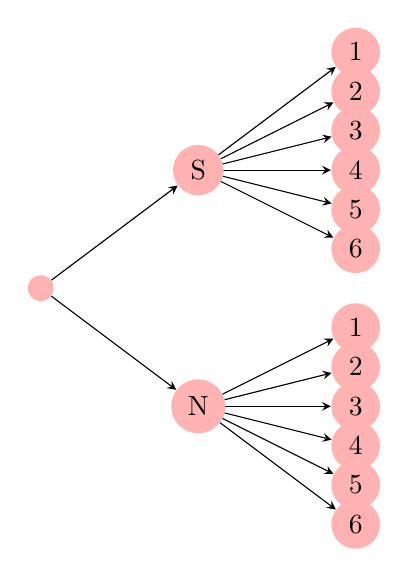
\begin{tikzpicture}[>=stealth,scale=1, line join=round, line cap=round]
				\node[circle, fill=red!30] (a) at (0,0)  {};
				\node[circle, fill=red!30] (b) at (2,1.5)  {\text{S}};
				\node[circle, fill=red!30] (c) at (2,-1.5)  {\text{N}};
				\node[circle, fill=red!30] (d1) at (4,3)  {$1$};
				\node[circle, fill=red!30] (d2) at (4,2.5)  {$2$};
				\node[circle, fill=red!30] (d3) at (4,2)  {$3$};
				\node[circle, fill=red!30] (d4) at (4,1.5)  {$4$};
				\node[circle, fill=red!30] (d5) at (4,1)  {$5$};
				\node[circle, fill=red!30] (d6) at (4,0.5)  {$6$};
				
				\node[circle, fill=red!30] (e1) at (4,-3)  {$6$};
				\node[circle, fill=red!30] (e2) at (4,-2.5)  {$5$};
				\node[circle, fill=red!30] (e3) at (4,-2)  {$4$};
				\node[circle, fill=red!30] (e4) at (4,-1.5)  {$3$};
				\node[circle, fill=red!30] (e5) at (4,-1)  {$2$};
				\node[circle, fill=red!30] (e6) at (4,-0.5)  {$1$};
				\draw[->](a)--(b);\draw[->](a)--(c);
				\draw[->](b)--(d1);\draw[->](b)--(d2);\draw[->](b)--(d3);\draw[->](b)--(d4);\draw[->](b)--(d5);\draw[->](b)--(d6);
				\draw[->](c)--(e1);\draw[->](c)--(e2);\draw[->](c)--(e3);\draw[->](c)--(e4);\draw[->](c)--(e5);\draw[->](c)--(e6);
			\end{tikzpicture}
		}
	}
\end{vd}

% #1492 | Archive/2024/Update-SP-BG10-11-3/SP-3/BG11-3/data_1C5/DS11-C5-B2-Dang6-SoDoHinhCay-TranTony.tex | mã gốc 1D9H2-5
\begin{vd}%[Bài giảng 11, Trần Tony]%[1D9H2-5]
	Vẽ sơ đồ hình cây để chọn ra $2$ bạn để phân công trực nhật trong một tổ có $4$ nam và $5$ nữ. 
	\loigiai{
		Dựa vào yêu cầu bài toán, ta có sơ đồ hình cây sau:
		\begin{center}
			\begin{tikzpicture}[scale=0.2,>=stealth,every node/.style={shape=rectangle,draw,rounded corners, color=blue, fill=blue!10}]
				%-------------
				\tikzstyle{block} = [rectangle, draw, fill=blue!10, rounded corners, text centered, text width = 9em, minimum height = 1em]
				%-------------
				\node (c1) [block] {Lấy ngẫu nhiên $2$ bạn trong tổ};
				\node (c2) [block, below right = 1.5cm of c1]{Lấy $2$ bạn nam ($\mathrm{C_4^2}$)};
				\node (c3) [block, below= 0.6cm of c1]{Lấy $1$ bạn nam ($\mathrm{C_4^1}$)};
				\node (c4) [block, below left= 1.5cm of c1]{Lấy $2$ bạn nữ ($\mathrm{C_5^2}$)};
				\node (c5) [block,below = 1cm of c2]{Có $6$ cách};
				\node (c6) [block,below = 0.5cm of c3]{Lấy $1$ bạn nữ ($\mathrm{C_5^1}$)};
				\node (c7) [block,below = 1cm of c4]{Có $10$ cách};
				\node (c8) [block,below = 0.5cm of c6]{Có $\mathrm{C_4^1}\cdot\mathrm{C_5^1}$ cách};
				%--------------
				\draw[->] (c1.south) -- (c2.north);
				\draw[->] (c1.south) -- (c3.north);
				\draw[->] (c1.south) -- (c4.north);
				\draw[->] (c2.south) -- (c5.north);
				\draw[->] (c3.south) -- (c6.north);
				\draw[->] (c4.south) -- (c7.north);
				\draw[->] (c6.south) -- (c8.north);
			\end{tikzpicture}
		\end{center}
		Theo sơ đồ hình cây trên thì số phần tử của không gian mẫu của phép thử là\\ $n({\Omega})=10+\mathrm{C_5^1}\cdot\mathrm{C_4^1}+6=36$.
	}
\end{vd}

% #1493 | Archive/2024/Update-SP-BG10-11-3/SP-3/BG11-3/data_1C5/DS11-C5-B2-Dang6-SoDoHinhCay-TranTony.tex | mã gốc 1D9H2-5
\begin{vd}%[Bài giảng 11, Trần Tony]%[1D9H2-5]
	Một hộp chứa $7$ quả cầu đỏ và $5$ quả cầu xanh. Lấy ngẫu nhiên từ hộp ra $3$ quả cầu, sử dụng sơ đồ hình cây mô tả số phần tử của không gian mẫu của phép thử.
	\loigiai{ Dựa vào yêu cầu bài toán, ta có sơ đồ hình cây sau:
		\begin{center}
			\begin{tikzpicture}[scale=.2,>=stealth,every node/.style={shape=rectangle,draw,rounded corners, color=blue, fill=blue!10}]
				%-------------
				\tikzstyle{block} = [rectangle, draw, fill=blue!10, rounded corners, text centered, text width = 9em, minimum height = 2em]
				%-------------
				\node (c1)[block] {Lấy ngẫu nhiên $3$ quả cầu từ trong hộp};
				\node (tmp) [below = 2cm of c1, inner sep=0, minimum size=0pt] {};
				\node (c2) [block, right = 4.8cm of tmp]{Lấy $3$ quả màu đỏ\\ ($\mathrm{C_7^3}$)};
				\node (c3) [block, left = 4.8cm of tmp]{Lấy $3$ quả màu xanh ($\mathrm{C_5^3}$)};
				\node (c4) [block, left = 0.3cm of c2]{Lấy $2$ quả màu đỏ\\  ($\mathrm{C_7^2}$)};
				\node (c5) [block, right = 0.3cm of c3]{Lấy $2$ quả màu xanh ($\mathrm{C_5^2}$)};
				\node (c6) [block,below =3cm of c2]{Có $35$ cách};
				\node (c7) [block, below = 3cm of c3]{Có $10$ cách};
				\node (c8) [block, below = 1cm of c4]{Lấy $1$ quả màu xanh ($\mathrm{C_5^1}$)};
				\node (c9) [block, below = 1cm of c5]{Lấy $1$ quả màu đỏ \\ ($\mathrm{C_7^1}$)};
				\node (c10) [below = 1cm of c9]{Có $\mathrm{C_7^1}\cdot\mathrm{C_5^2}$ cách};
				\node (c11) [below = 1cm of c8]{Có $\mathrm{C_5^1}\cdot\mathrm{C_7^2}$ cách};
				%--------------
				\draw[->] (c1.south) -- (c2.north);
				\draw[->] (c1.south) -- (c3.north);
				\draw[->] (c1.south) -- (c4.north);
				\draw[->] (c1.south) -- (c5.north);
				\draw[->] (c2.south) -- (c6.north);
				\draw[->] (c3.south) -- (c7.north);
				\draw[->] (c4.south) -- (c8.north);
				\draw[->] (c5.south) -- (c9.north);	
				\draw[->] (c9.south) -- (c10.north);
				\draw[->] (c8.south) -- (c11.north);
			\end{tikzpicture}
		\end{center}
		Theo sơ đồ hình cây trên thì số phần tử của không gian mẫu của phép thử là $$n({\Omega})=10+\mathrm{C_5^1}\cdot\mathrm{C_7^2}+\mathrm{C_5^2}\cdot\mathrm{C_7^1}+35=220.$$
	}
\end{vd}

% #1494 | Archive/2024/Update-SP-BG10-11-3/SP-3/BG11-3/data_1C5/DS11-C5-B2-Dang6-SoDoHinhCay-TranTony.tex | mã gốc 1D9H2-5
\begin{bt}%[Bài giảng 11, Trần Tony]%[1D9H2-5]
	Một hộp chứa $5$ quả cầu màu xanh và $8$ quả cầu màu đỏ. Lập sơ đồ hình cây của biến cố A "Lấy được $3$ quả cầu và có đủ cả hai màu".
	\loigiai{
		Dựa vào yêu cầu bài toán, ta có sơ đồ hình cây sau:
		\begin{center}
			\begin{tikzpicture}[scale=0.2,>=stealth,every node/.style={shape=rectangle,draw,rounded corners, color=blue, fill=blue!10}]
				%-------------
				\tikzstyle{block} = [rectangle, draw, fill=blue!10, rounded corners, text centered, text width = 10em, minimum height = 2em]
				%-------------
				\node (c1) [block] {Lấy ngẫu nhiên $3$ quả cầu và có đủ cả hai màu};
				\node (c2) [block, below right = 1cm of c1]{Lấy $1$ quả cầu màu đỏ\\ ($\mathrm{C_8^1}$)};
				\node (c3) [block, below left= 1cm of c1]{Lấy $2$ quả cầu màu đỏ\\ ($\mathrm{C_8^2}$)};
				\node (c4) [block,below = 1cm of c2]{Lấy $2$ quả cầu màu xanh\\ ($\mathrm{C_5^2}$)};
				\node (c5) [block,below = 1cm of c3]{Lấy $1$ quả cầu màu xanh\\ ($\mathrm{C_5^1}$)};
				\node (c6) [block,below = 1cm of c4]{Có $\mathrm{C_8^1}\cdot\mathrm{C_5^2}$ cách};
				\node (c7) [block,below = 1cm of c5]{Có $\mathrm{C_8^2}\cdot\mathrm{C_5^1}$ cách};
				%--------------
				\draw[->] (c1.south) -- (c2.north);
				\draw[->] (c1.south) -- (c3.north);
				\draw[->] (c2.south) -- (c4.north);
				\draw[->] (c3.south) -- (c5.north);
				\draw[->] (c4.south) -- (c6.north);
				\draw[->] (c5.south) -- (c7.north);
			\end{tikzpicture}
		\end{center}
		Vậy số phần tử của biến cố A là $n_{(\mathrm{A})}=\mathrm{C_8^1}\cdot\mathrm{C_5^2}+\mathrm{C_8^2}\cdot\mathrm{C_5^1}=220$.
	}
\end{bt}

% #1495 | Archive/2024/Update-SP-BG10-11-3/SP-3/BG11-3/data_1C5/DS11-C5-B2-Dang6-SoDoHinhCay-TranTony.tex | mã gốc 1D9H2-5
\begin{bt}%[Bài giảng 11, Trần Tony]%[1D9H2-5]
	Trong một ngân hàng đề kiểm tra có ba loại câu hỏi dễ - trung bình - khó. Biết loại dễ có $10$ câu, loại trung bình có $8$ câu và loại khó có $4$ câu. Giáo viên cần tạo ra một đề thi có $3$ câu từ ngân ngàng đề thi đó. Lập sơ đồ hình cây cho biến cố "Đề thi được tạo thành có đúng $2$ loại câu hỏi".
	\loigiai{
		Dựa vào yêu cầu bài toán, ta có sơ đồ hình cây sau:
		\begin{center}
			\begin{tikzpicture}[scale=.2,>=stealth,every node/.style={shape=rectangle,draw,rounded corners, color=blue, fill=blue!10}]
				%-------------
				\tikzstyle{block} = [rectangle, draw, fill=blue!10, rounded corners, text centered, text width = 6em, minimum height = 3em]
				%------------- cấp 1
				\node (c1) [block] {Lấy ngẫu nhiên $3$\\ câu hỏi chỉ thuộc $2$ loại câu hỏi};
				\node (c2) [block, above right = 1cm of c1]{Lấy $1$ câu hỏi dễ\\ có $10$ cách};
				\node (c3) [block, right= 0.7cm of c1]{Lấy $1$ câu hỏi trung bình\\ có $8$ cách};
				\node (c4) [block, below right= 1cm of c1]{Lấy $1$ câu hỏi khó\\ có $4$ cách};
				%--------------- cấp 2
				\node (c5) [block,below right = 3.5cm of c2]{Lấy $2$ câu hỏi trung bình có $\mathrm{C_8^2}$\\cách chọn};
				\node (c6) [block,above right= 3.5cm of c2]{Lấy $2$ câu hỏi khó\\ có $\mathrm{C_4^2}$\\cách chọn};
				\node (c7) [block,below right = 3.5cm of c3]{Lấy $2$ câu hỏi dễ\\ có $\mathrm{C_{10}^2}$\\cách chọn};
				\node (c8) [block,above right= 3.5cm of c3]{Lấy $2$ câu hỏi khó\\ có $\mathrm{C_4^2}$\\cách chọn};
				\node (c9) [block,below right = 3.5cm of c4]{Lấy $2$ câu hỏi trung bình\\ có $\mathrm{C_8^2}$\\cách chọn};
				\node (c10) [block,above right= 3.5cm of c4]{Lấy $2$ câu hỏi dễ\\ có $\mathrm{C_{10}^2}$\\cách chọn};
				%-------------- cấp 3
				\node (c11) [block,right = 0.5cm of c5]{Vậy có $10\cdot\mathrm{C_8^2}$ cách chọn};
				\node (c12) [block,right = 0.5cm of c6]{Vậy có $10\cdot\mathrm{C_4^2}$ cách chọn};
				\node (c13) [block,right = 0.5cm of c7]{Vậy có $8\cdot\mathrm{C_{10}^2}$ cách chọn};
				\node (c14) [block,right = 0.5cm of c8]{Vậy có $8\cdot\mathrm{C_4^2}$ cách chọn};
				\node (c15) [block,right = 0.5cm of c9]{Vậy có $4\cdot\mathrm{C_{8}^2}$ cách chọn};
				\node (c16) [block,right = 0.5cm of c10]{Vậy có $4\cdot\mathrm{C_{10}^2}$ cách chọn};
				%--------------- các đường nối các block
				\draw[->] (c1.east) -- (c2.west);
				\draw[->] (c1.east) -- (c3.west);
				\draw[->] (c1.east) -- (c4.west);
				\draw[->] (c2.east) -- (c5.west);
				\draw[->] (c2.east) -- (c6.west);
				\draw[->] (c3.east) -- (c7.west);
				\draw[->] (c3.east) -- (c8.west);
				\draw[->] (c4.east) -- (c9.west);
				\draw[->] (c4.east) -- (c10.west);
				\draw[->] (c5.east) -- (c11.west);
				\draw[->] (c6.east) -- (c12.west);
				\draw[->] (c7.east) -- (c13.west);
				\draw[->] (c8.east) -- (c14.west);
				\draw[->] (c9.east) -- (c15.west);
				\draw[->] (c10.east) -- (c16.west);
			\end{tikzpicture}
		\end{center}
		Vậy số phần tử của biến cố cần tìm là $10\cdot\mathrm{C_8^2}+10\cdot\mathrm{C_4^2}+8\cdot\mathrm{C_{10}^2}+8\cdot\mathrm{C_4^2}+4\cdot\mathrm{C_{8}^2}+4\cdot\mathrm{C_{10}^2}=1040 $.
	}
\end{bt}

% #1496 | Archive/2024/Update-SP-BG10-11-3/SP-3/BG11-3/data_1C5/DS11-C5-B2-Dang6-SoDoHinhCay-TranTony.tex | mã gốc 1D9H2-5
\begin{bt}%[Bài giảng 11, Trần Tony]%[1D9H2-5]
	Rút ngẫu nhiên $4$ lá bài từ một bộ bài Tây. Lập sơ đồ hình cây cho biến cố $\mathrm{A}\colon$ "Rút được ít nhất $2$ con Át".
	\loigiai{
		Dựa vào yêu cầu bài toán, ta có sơ đồ hình cây sau:
		\begin{center}
			\begin{tikzpicture}[scale=.3,>=stealth,every node/.style={shape=rectangle,draw,rounded corners, color=blue, fill=blue!10}]
				%-------------
				\tikzstyle{block} = [rectangle, draw, fill=blue!10, rounded corners, text centered, text width = 6em, minimum height = 3em]
				%------------- cấp 1
				\node (c1) [block] {Lấy được ít nhất $2$ quân Át};
				\node (c2) [block, above right = 1cm of c1]{Lấy $2$ quân Át có $\mathrm{C_4^2}$ cách lấy};
				\node (c3) [block, right= 0.7cm of c1]{Lấy $3$ quân Át có $\mathrm{C_4^3}$ cách lấy};
				\node (c4) [block, below right= 1cm of c1]{Lấy $4$ quân Át có $1$ cách lấy};
				%--------------- cấp 2
				\node (c5) [block,right = 1cm of c2]{Lấy $2$ quân bất kỳ còn lại có $\mathrm{C_{48}^2}$ cách lấy};
				\node (c6) [block,right = 1cm of c3]{Lấy $1$ quân bất kỳ còn lại có $\mathrm{C_{48}^1}$ cách lấy};
				\node (c7) [block,right = 4cm of c4]{Có $1$ cách lấy};
				%................ cấp 3
				\node (c8) [block,right = 1cm of c5]{Có $\mathrm{C_4^2}\cdot\mathrm{C_{48}^2}$ cách lấy};
				\node (c9) [block,right = 1cm of c6]{Có $\mathrm{C_4^3}\cdot\mathrm{C_{48}^1}$ cách lấy};
				%--------------- các đường nối các block
				\draw[->] (c1.east) -- (c2.west);
				\draw[->] (c1.east) -- (c3.west);
				\draw[->] (c1.east) -- (c4.west);
				\draw[->] (c2.east) -- (c5.west);
				\draw[->] (c3.east) -- (c6.west);
				\draw[->] (c4.east) -- (c7.west);
				\draw[->] (c5.east) -- (c8.west);
				\draw[->] (c6.east) -- (c9.west);
			\end{tikzpicture}
		\end{center}
		Vậy số phần tử của biến cố cần tìm là\\
		$n{(\mathrm{A})}=1+ \mathrm{C_4^2}\cdot\mathrm{C_{48}^2} + \mathrm{C_4^3}\cdot\mathrm{C_{48}^1}=6961$.
	}
\end{bt}

% #1497 | Archive/2024/Update-SP-BG10-11-3/SP-3/BG11-3/data_1C5/DS11-C5-B2-Dang6-SoDoHinhCay-TranTony.tex | mã gốc 1D9H2-5
\begin{bt}%[Bài giảng 11, Trần Tony]%[1D9H2-5]
	Câu lạc bộ nghệ thuật của một trường trung học phổ thông gồm học sinh của cả ba khối $10$, $11$, $12$, mỗi khối có $5$ học sinh. Chọn ngẫu nhiên $3$ học sinh để tham gia biểu diễn. Tính xác suất để $3$ học sinh được chọn chỉ thuộc hai khối.
	\loigiai{
	Mỗi cách chọn ra đồng thời $3$ học sinh trong câu lạc bộ cho ta một tổ hợp chập $3$ của $15$ phần tử. Do đó, không gian mẫu $\Omega$ gồm các tổ hợp chập $3$ của $15$ phần tử và
	$$
	n(\Omega)=\mathrm{C}_{15}^3=\dfrac{15!}{3!\cdot 12!}=455.
	$$
	Xét biến cố $A$: "Chọn được $3$ học sinh chỉ thuộc hai khối".\\
	Sơ đồ hình cây biểu thị các khả năng thuận lợi cho biến cố $A$.
	\begin{center}
		\begin{tikzpicture}[scale=0.7,>=stealth,every node/.style={rectangle,draw,rounded corners, text centered, text width=6em, fill=orange!20}]
			% Define block styles
			\tikzstyle{block} = [rectangle, draw, fill=orange!20, rounded corners, text centered, text width=3em, minimum height=2em]
			\tikzstyle{blockn} = [rectangle, draw, fill=orange!20, rounded corners, text centered, text width=5em, minimum height=2em]
			% Nodes
			\node (c1) [blockn] {Chọn 3 học sinh (HS) chỉ ở hai khối};
			
			\node (c2) [blockn, below left= 0.5cm and 3.5cm of c1]{Chọn 1 HS lớp 10:\\Có 5 cách chọn};
			\node (c3) [blockn, below = 0.5cm of c1]{Chọn 1 HS lớp 11:\\Có 5 cách chọn};
			\node (c4) [blockn, below right = 0.5cm and 3.5cm of c1]{Chọn 1 HS lớp 12:\\Có 5 cách chọn};
			
			\node (c5) [block, below left = 0.4cm and 0cm of c2]{Chọn 2 HS lớp 11:\\Có $C_5^2$ cách chọn};
			\node (c6) [block, below right = 0.4cm and 0cm of c2]{Chọn 2 HS lớp 12:\\Có $C_5^2$ cách chọn};
			
			\node (c7) [block, below left = 0.4cm and 0cm of c3]{Chọn 2 HS lớp 10:\\Có $C_5^2$ cách chọn};
			\node (c8) [block, below right = 0.4cm and 0cm of c3]{Chọn 2 HS lớp 12:\\Có $C_5^2$ cách chọn};
			
			\node (c9) [block, below left = 0.4cm and 0cm of c4]{Chọn 2 HS lớp 10:\\Có $C_5^2$ cách chọn};
			\node (c10) [block, below right = 0.4cm and 0cm of c4]{Chọn 2 HS lớp 11:\\Có $C_5^2$ cách chọn};
			
			\node (c11) [block, below = 0.5cm of c5]{Có $5\cdot C_5^2 = 50$ cách chọn};
			\node (c12) [block, below = 0.5cm of c6]{Có $5\cdot C_5^2 = 50$ cách chọn};
			
			\node (c13) [block, below = 0.5cm of c7]{Có $5\cdot C_5^2 = 50$ cách chọn};
			\node (c14) [block, below = 0.5cm of c8]{Có $5\cdot C_5^2 = 50$ cách chọn};
			
			\node (c15) [block, below = 0.5cm of c9]{Có $5\cdot C_5^2 = 50$ cách chọn};
			\node (c16) [block, below = 0.5cm of c10]{Có $5\cdot C_5^2 = 50$ cách chọn};
			
			% Arrows
			\draw[->] (c1.south) -- (c2.north);
			\draw[->] (c1.south) -- (c3.north);
			\draw[->] (c1.south) -- (c4.north);
			
			\draw[->] (c2.south) -- (c5.north);
			\draw[->] (c2.south) -- (c6.north);
			
			\draw[->] (c3.south) -- (c7.north);
			\draw[->] (c3.south) -- (c8.north);
			
			\draw[->] (c4.south) -- (c9.north);
			\draw[->] (c4.south) -- (c10.north);
			
			\draw[->] (c5.south) -- (c11.north);
			\draw[->] (c6.south) -- (c12.north);
			
			\draw[->] (c7.south) -- (c13.north);
			\draw[->] (c8.south) -- (c14.north);
			
			\draw[->] (c9.south) -- (c15.north);
			\draw[->] (c10.south) -- (c16.north);
		\end{tikzpicture}
	\end{center}
	Như vậy, số kết quả thuận lợi cho biến cố $A$ là $n(A)=50\cdot 6=300$.\\
	Vậy xác suất của biến cố $A$ là
	$$
	\mathrm{P}(A)=\dfrac{n(A)}{n(\Omega)}=\dfrac{300}{455}=\dfrac{60}{91}.
	$$
	}
\end{bt}

% #1498 | Archive/2024/Update-SP-BG10-11-3/SP-3/BG11-3/data_1C5/DS11-C5-B2-Dang6-SoDoHinhCay-TranTony.tex | mã gốc 1D9H2-5
\begin{ex}%[Bài giảng 11, Trần Tony]%[1D9H2-5]
	\immini{Hai bạn An và Bình không quen biết nhau và đều học xa nhà. Xác suất của biến cố $A$: "An về thăm nhà vào ngày Chủ nhật" là $0{,}2$ và của biến cố $B$: "Bình về thăm nhà vào Chủ nhật" là $0{,}25$. Ta có sơ đồ hình cây để tính xác suất vào ngày Chủ nhật:
	}{
	\begin{tikzpicture}[line join=round, line cap=round,yscale=0.9]
		\draw[->] (0,5)node[above]{Xác suất}--(-2.5,4)node[below]{$A$};
		\draw[->] (0,5)--(2.5,4)node[below]{$\overline{A}$};
		\draw[->] (-2.5,3)--(-3.5,2)node[below]{$B$};
		\draw[->] (-2.5,3)--(-1.5,2)node[below]{$\overline{B}$};
		\draw[->] (2.5,3)--(1.5,2)node[below]{$B$};
		\draw[->] (2.5,3)--(3.5,2)node[below]{$\overline{B}$};
		\draw (-1.5,4.6) node{$0{,}2$} (1.5,4.6) node{$0{,}8$};
		\draw (-3.5,2.5) node{$0{,}25$} (-1.5,2.5) node{$0{,}75$};
		\draw (1.5,2.5) node{$0{,}25$} (3.7,2.5) node{$X=?$};
		\end{tikzpicture}
	}
	\choiceTF[t]
	{\True Cả hai bạn đều về thăm nhà là $0{,}05$}
	{Có ít nhất một bạn về thăm nhà là $0{,}45$}
	%{\True Cả hai bạn đều không về thăm nhà là $0{,}6$}
	%{\True Chỉ có bạn An về thăm nhà là $0{,}15$}
	{Trong sơ đồ hình cây, giá trị $X$ là $X=0{,}8$}
	{\True Có đúng một bạn về thăm nhà là $0{,}35$}
	\loigiai{
	\begin{itemchoice}
		\itemch 
		Xác suất của biến cố "Cả hai bạn đều về thăm nhà" là $$P(A\cap B)=P(AB)=P(A)P(B)=0{,}2\cdot 0{,}25=0{,}05.$$
		\itemch 
			Xác suất của biến cố "Có ít nhất một bạn về thăm nhà" là $$P(A\cup B)=P(A)+P(B)-P(A\cap B)=0{,}2+0{,}25-0{,}05=0{,}4.$$
		\itemch 
		Trong sơ đồ hình cây, giá trị $X$ là $X=1-0{,}25=0{,}75$.
		\itemch 
		Xác suất của biến cố "Có đúng một bạn về thăm nhà" là $$P=P(A\overline{B}\cup \overline{A}B)=P(A\overline{B})+P(\overline{A}B)=0{,}2\cdot 0{,}75 +0{,}8\cdot 0{,}25=0{,}35.$$
	\end{itemchoice}
	}
\end{ex}

% #1499 | Archive/2024/Update-SP-BG10-11-3/SP-3/BG11-3/data_1C5/DS11-C5-B2-Dang6-SoDoHinhCay-TranTony.tex | mã gốc 1D9V2-5
\begin{ex}%[Bài giảng 11, Trần Tony]%[1D9V2-5]
	Ba xạ thủ cùng bắn, mỗi người một viên đạn vào bia một cách độc lập với nhau. Xác suất bắn trúng bia của ba xạ thủ lần lượt là $\dfrac{1}{2}; \dfrac{1}{4}$ và $\dfrac{1}{3}$. Tính xác suất của biến cố có ít nhất hai xạ thủ không bắn trúng bia (kết quả làm tròn tới hàng phần trăm).
	\shortans{$0{,}86$}
	\loigiai
	{
	Giả sử $A:$\lq\lq Xạ thủ $1$ bắn trúng bia \rq\rq.\\
	Suy ra $\mathrm{P}(A)=\dfrac{1}{2}\Rightarrow \mathrm{P}(\overline{A})=1-\mathrm{P}(A)=1-\dfrac{1}{2}=\dfrac{1}{2}$.\\
	Giả sử $B:$\lq\lq Xạ thủ hai bắn trúng bia \rq\rq.\\
	Suy ra $\mathrm{P}(B)=\dfrac{1}{4}\Rightarrow \mathrm{P}(\overline{B})=1-\mathrm{P}(B)=1-\dfrac{1}{4}=\dfrac{3}{4}$.\\
	Giả sử $C:$ \lq\lq Xạ thủ ba bắn trúng bia \rq\rq.\\
	Suy ra $\mathrm{P}(C)=\dfrac{1}{3}\Rightarrow \mathrm{P}(\overline{C})=1-\mathrm{P}(C)=1-\dfrac{1}{3}=\dfrac{2}{3}$.\\
	Nhận thấy $A, B, C$ là các biến cố độc lập nên suy ra $A, B, C, \overline{A}, \overline{B},\overline{C}$ đôi một độc lập với nhau.\\
	Ta có sơ đồ sau
	\begin{center}
		\begin{tikzpicture}[line join=round, line cap=round,thick,xscale=1,yscale=0.7]
			\draw[->] (0,5)node[above]{Gốc}--(-2.5,4)node[below]{$A$};
			\draw[->] (0,5)--(2.5,4)node[below]{$\overline{A}$};
			\draw[->] (-2.5,3)--(-3.5,2)node[below]{$B$};
			\draw[->] (-2.5,3)--(-1.5,2)node[below]{$\overline{B}$};
			\draw[->] (2.5,3)--(3.5,2)node[below]{$B$};
			\draw[->] (2.5,3)--(1.5,2)node[below]{$\overline{B}$};
			
			\draw[->] (-3.5,1)--(-4,0)node[below]{$C$};
			\draw[->] (-3.5,1)--(-3,0)node[below]{$\overline{C}$};
			
			\draw[->] (-1.5,1)--(-2,0)node[below]{$C$};
			\draw[->] (-1.5,1)--(-1,0)node[below]{$\overline{C}$};
			
			\draw[->] (1.5,1)--(1,0)node[below]{$C$};
			\draw[->] (1.5,1)--(2,0)node[below]{$\overline{C}$};
			
			\draw[->] (3.5,1)--(3,0)node[below]{$C$};
			\draw[->] (3.5,1)--(4,0)node[below]{$\overline{C}$};
		\end{tikzpicture}
	\end{center}
		Gọi $D:$\lq\lq Có ít nhất hai xạ thủ không bắn trúng bia \rq\rq.\\
		Suy ra $D=\{(A\overline{BC}), (\overline{A}B\overline{C}), (\overline{AB}C), (\overline{ABC})\}$.\\
		Suy ra 
		\begin{align*}
			\mathrm{P}(D)=&\, \mathrm{P}(A\overline{BC})+\mathrm{P}(\overline{A}B\overline{C})+P\mathrm{P}(\overline{AB}C)+\mathrm{P}(\overline{ABC})\\
			=&\, \dfrac{1}{2}\cdot\dfrac{3}{4}\cdot\dfrac{2}{3}+\dfrac{1}{2}\cdot\dfrac{1}{3}\cdot\dfrac{2}{3}+\dfrac{1}{2}\cdot\dfrac{3}{4}\cdot\dfrac{1}{3}+\dfrac{1}{2}\cdot\dfrac{3}{4}\cdot\dfrac{2}{3}\\
			=&\, \dfrac{1}{4}+\dfrac{1}{9}+\dfrac{1}{8}+\dfrac{1}{4}\\
			=&\, \dfrac{31}{36}\approx 0{,}86.
		\end{align*}
		Vậy $\mathrm{P}(D)\approx 0{,}86$.
	}
\end{ex}

% #1539 | Archive/2024/Update-SP-BG10-11-3/SP-3/BG11-3/data_1C5/DS11-C5-B2-Dang7-TinhXacSuatBangKetHopCacQuyTac-TranTony.tex | mã gốc 1D9H2-6
\begin{vd}%[Bài giảng 11, Trần Tony]%[1D9H2-6]
	Một xưởng sản suất có hai chiếc máy chạy độc lập với nhau. Xác suất để máy $I$ và $II$ chạy tốt lần lượt là $0{,}7$ và $0{,}8$. Tính xác suất để xưởng chỉ có một máy chạy tốt.
	\loigiai{
		Gọi $\mathrm{P}(A)=0{,}7$ là xác suất để máy $I$ chạy tốt và $\mathrm{P}(B)=0{,}8$ là xác suất để máy $II$ chạy tốt, $\mathrm{P}(C)$ là xác suất để xưởng chỉ có một máy chạy tốt.\\
		Khi đó, xác suất để máy $I$ và máy $II$ hỏng là $\mathrm{P}\left(\overline{A}\right)=0{,}3$, $\mathrm{P}\left(\overline{B}\right)=0{,}2$.\\
		Vì hai máy là độc lập nhau nên ta có $\mathrm{P}(C)=\mathrm{P}\left(A\cap \overline{B}\right)+\mathrm{P}\left(\overline{A}\cap B\right)=0{,}3\cdot0{,}8+0{,}7\cdot 0{,}2=0{,}38$.
	}
\end{vd}

% #1540 | Archive/2024/Update-SP-BG10-11-3/SP-3/BG11-3/data_1C5/DS11-C5-B2-Dang7-TinhXacSuatBangKetHopCacQuyTac-TranTony.tex | mã gốc 1D9H2-6
\begin{vd}%[Bài giảng 11, Trần Tony]%[1D9H2-6]
	Hai vận động viên cùng bắn vào bia, biết xác suất bắn trúng hồng tâm của hai vận động viên $I$ và $II$ lần lượt là $0{,}7$ và $0{,}9$. Tính xác suất để một vận động viên đều bắn trượt hồng tâm của bia.
	\loigiai{
		Gọi $\mathrm{P}(A)=0{,}7$ là xác suất bắn trúng hồng tâm của bia của vận động viên số $I$. Vậy xác suất bắn trượt hồng tâm của bia của vđv $I$ là $\mathrm{P}\left(\overline{A}\right)=0{,}3$.\\
		Gọi $\mathrm{P}(B)=0{,}9$ là xác suất bắn trúng hồng tâm của bia của vận động viên số $II$. Vậy xác suất bắn trượt hồng tâm của bia của vđv $II$ là $\mathrm{P}\left(\overline{B}\right)=0{,}1$.\\
		Vì xác suất của hai vận động viên là độc lập với nhau nên để một vận động viên bắn trượt bia là
		$$\mathrm{P}\left(A\cap\overline{B}\right)+\mathrm{P}(\left(\overline{A}\cap B\right)=0{,}7\cdot0{,}1+0{,}3\cdot0{,}9=0{,}34.$$
	}
\end{vd}

% #1541 | Archive/2024/Update-SP-BG10-11-3/SP-3/BG11-3/data_1C5/DS11-C5-B2-Dang7-TinhXacSuatBangKetHopCacQuyTac-TranTony.tex | mã gốc 1D9H2-6
\begin{vd}%[Bài giảng 11, Trần Tony]%[1D9H2-6]
	Gieo hai đồng xu $A$ và $B$ một cách độc lập. Đồng xu $A$ chế tạo cân đối, đồng xu $B$ không cân đối nên xác suất xuất hiện mặt sấp gấp $3$ lần xác suất xuất hiện mặt ngửa.
	\choiceTF[t]
	{\True Xác suất để đồng xu $A$ xuất hiện mặt sấp là $\dfrac{1}{2}$}
	{Xác suất để đồng xu $B$ xuất hiện mặt sấp là $\dfrac{1}{2}$}
	{\True Xác suất để khi gieo hai đồng xu cùng lúc được kết quả hai đồng xu cùng sấp là $\dfrac{3}{8}$}
	{Xác suất để khi gieo hai đồng xu cùng lúc được kết quả một mặt sấp, một mặt ngửa lớn hơn $\dfrac{1}{2}$}
	\loigiai{
		Gọi $M$ là biến cố ``Đồng xu $A$ xuất hiện mặt sấp''.\\
		$N$ là biến cố ``Đồng xu $B$ xuất hiện mặt sấp''. \\
		Gọi $Y$ là biến cố ``Có một mặt sấp và một mặt ngửa xuất hiện khi gieo hai đồng xu cùng lúc''.\\
		Ta có $Y=M\overline{N}\cup \overline{M}N$. Mà $M\overline{N}$ và $\overline{M}N$ xung khắc nhau; $M$ và $\overline{N}$ độc lập; $\overline{M}$ và $N$ độc lập.\\
		Suy ra $\mathrm{P}(Y)=\mathrm{P}\left(M\overline{N}\right)+\mathrm{P}\left(\overline{M}N\right)=\mathrm{P}(M)\mathrm{P}\left(\overline{N}\right)+\mathrm{P}\left(\overline{M}\right)\mathrm{P}(N)=\dfrac{1}{2}\cdot \dfrac{1}{4}+\dfrac{1}{2}\cdot\dfrac{3}{4}=\dfrac{1}{2}$.
	\begin{itemchoice}
		\itemch 
		$\mathrm{P}(M)=\dfrac{1}{2}$.
		\itemch 
		Xác suất để đồng xu $B$ xuất hiện mặt sấp là $\mathrm{P}(N)=\dfrac{3}{4}$.
		\itemch 
		Xác suất để khi gieo hai đồng xu cùng lúc được kết quả hai đồng xu cùng sấp là $\mathrm{P}(M)\cdot \mathrm{P}(N)=\dfrac{1}{2}\cdot\dfrac{3}{4}=\dfrac{3}{8}$.
		\itemch 
		$\mathrm{P}(Y)=\dfrac{1}{2}$.
	\end{itemchoice}
	}
\end{vd}

% #1542 | Archive/2024/Update-SP-BG10-11-3/SP-3/BG11-3/data_1C5/DS11-C5-B2-Dang7-TinhXacSuatBangKetHopCacQuyTac-TranTony.tex | mã gốc 1D9H2-6
\begin{vd}%[Bài giảng 11, Trần Tony]%[1D9H2-6]
	Có $3$ chiếc hộp $A$, $B$, $C$. Hộp $A$ chứa $4$ bi đỏ, $3$ bi trắng. Hộp $B$ chứa $3$ bi đỏ, $2$ bi vàng. Hộp $C$ chứa $2$ bi đỏ, $2$ bi vàng. Lấy ngẫu nhiên một hộp từ $3$ hộp này, rồi lấy ngẫu nhiên một bi từ hộp đó. Tính xác suất để lấy được một bi đỏ (kết quả làm tròn đến hàng phần trăm).
	\shortans{$0{,}56$}
	\loigiai{
		Xác suất để chọn hộp $A$ là $\dfrac{1}{3}$, xác suất để chọn được bi đỏ trong hộp $A$ là $\dfrac{4}{7}$.\\
		Suy ra xác suất để chọn được bi đỏ trong hộp $A$ là $\dfrac{1}{3}\cdot \dfrac{4}{7}$.\\
		Tương tự, xác suất để chọn được bi đỏ trong hộp $B$, hộp $C$ lần lượt là $\dfrac{1}{3}\cdot \dfrac{3}{5}$, $\dfrac{1}{3}\cdot \dfrac{2}{4}$.\\
		Vậy xác suất để lấy được bi đỏ là $\mathrm{P}=\dfrac{1}{3}\cdot \dfrac{4}{7}+\dfrac{1}{3}\cdot \dfrac{3}{5}+\dfrac{1}{3}\cdot \dfrac{2}{4}=\dfrac{39}{70}\approx 0{,}56$.
	}
\end{vd}

% #1543 | Archive/2024/Update-SP-BG10-11-3/SP-3/BG11-3/data_1C5/DS11-C5-B2-Dang7-TinhXacSuatBangKetHopCacQuyTac-TranTony.tex | mã gốc 1D9H2-6
\begin{bt}%[Bài giảng 11, Trần Tony]%[1D9H2-6]
	Một hộp chứa $15$ quả cầu gồm $4$ quả cầu màu xanh, $3$ quả cầu màu vàng và $8$ quả cầu màu đỏ. Chọn ngẫu nhiên đồng thời $3$ quả cầu từ hộp đó. Tính xác suất để $3$ quả cầu chọn ra có ít nhất một quả cầu màu đỏ.
	\loigiai{
		Có $\mathrm{C}_{15}^3$ cách chọn ra $3$ quả trong $15$ quả cầu. \\Có $\mathrm{C}_7^3$ cách chọn ra $3$ quả trong $15$ quả cầu mà không có quả nào màu đỏ. \\
		Do vậy, có $\mathrm{C}_{15}^3-\mathrm{C}_7^3=420$ cách chọn ra $3$ quả cầu trong $15$ quả cầu mà có ít nhất một quả màu đỏ.
		\\Vậy, xác xuất để $3$ quả cầu chọn ra có ít nhất một quả cầu màu đỏ bằng $\mathrm{P}=\dfrac{420}{\mathrm{C}_{15}^3}=\dfrac{12}{13}$.
	}
\end{bt}

% #1544 | Archive/2024/Update-SP-BG10-11-3/SP-3/BG11-3/data_1C5/DS11-C5-B2-Dang7-TinhXacSuatBangKetHopCacQuyTac-TranTony.tex | mã gốc 1D9H2-6
\begin{bt}%[Bài giảng 11, Trần Tony]%[1D9H2-6]
	Một nhóm gồm $6$ học sinh nam và $4$ học sinh nữ. Chọn ngẫu nhiên đồng thời $3$ học sinh trong nhóm đó. Tính xác suất trong $3$ học sinh được chọn luôn có học sinh nữ.
	\loigiai{
		Gọi $\Omega$ là không gian mẫu.\\
		Ta có số phần tử của không gian mẫu: $n(\Omega) =\mathrm{C}_{10}^3$.\\
		Gọi $A$ là biến	cố trong $3$ học sinh được chọn luôn có học sinh nữ.\\
		Suy ra $\overline{A}$ là biến cố trong $3$ học sinh được chọn không có học sinh nữ.
		\begin{center}
			$\begin{array}{ll}
				&n(\overline{A})=\mathrm{C}_6^3\\
				\Rightarrow & P(\overline{A})=\dfrac{n(\overline{A})}{n(\Omega)}=\dfrac{\mathrm{C}_6^3}{\mathrm{C}_{10}^3}=\dfrac{1}{5}\\
				\Rightarrow &P(A)=1-P(\overline{A})=1-\dfrac{1}{6}=\dfrac{5}{6}.
			\end{array}$
		\end{center}
	}
\end{bt}

% #1545 | Archive/2024/Update-SP-BG10-11-3/SP-3/BG11-3/data_1C5/DS11-C5-B2-Dang7-TinhXacSuatBangKetHopCacQuyTac-TranTony.tex | mã gốc 1D9H2-6
\begin{bt}%[Bài giảng 11, Trần Tony]%[1D9H2-6]
	Đầu tiết học, cô giáo kiểm tra bài cũ bằng cách gọi lần lượt từng người từ đầu danh sách lớp lên bảng trả lời câu hỏi. Biết rằng các học sinh đầu tiên trong danh sách lớp là An, Bình, Cường với xác suất thuộc bài lần lượt là $0{,}9$, $0{,}7$ và $0{,}8$. Cô giáo sẽ dừng kiểm tra sau khi có hai học sinh thuộc bài. Tính xác suất cô giáo chỉ kiểm tra bài cũ đúng ba bạn trên.
	\loigiai{
		Cô giáo chỉ kiểm tra bài cũ đúng ba bạn trên khi xảy ra hai trường hợp sau:
		\begin{itemize}
			\item An thuộc bài, Bình không thuộc bài, Cường thuộc bài. Xác suất của trường hợp này là: $0{,}9\cdot 0{,}3\cdot 0{,}8=0{,}216$.
			\item An không thuộc bài, Bình thuộc bài, Cường thuộc bài. Xác suất của trường hợp này là: $0{,}1\cdot 0{,}7\cdot 0{,}8=0{,}056$.
		\end{itemize}
		Vậy xác suất cần tìm là $0{,}216+0{,}056=0{,}272$.
	}
\end{bt}

% #1546 | Archive/2024/Update-SP-BG10-11-3/SP-3/BG11-3/data_1C5/DS11-C5-B2-Dang7-TinhXacSuatBangKetHopCacQuyTac-TranTony.tex | mã gốc 1D9H2-6
\begin{bt}%[Bài giảng 11, Trần Tony]%[1D9H2-6]
	Trong một kỳ thi có $60$\% thí sinh đỗ. Hai bạn A, B cùng tham dự kỳ thi đó. Tính xác suất để chỉ có một bạn thi đỗ.
	\loigiai{
		Gọi $A$, $B$ lần lượt là các biến cố bạn A, B thi đỗ. Suy ra $\mathrm{P}(A)=0{,}6$, $\mathrm{P}(B)=0{,}6$.\\
		Gọi $C$ là biến cố chỉ một bạn thi đỗ. Suy ra $\mathrm{P}(C)=\mathrm{P}(A)\cdot \mathrm{P}(\overline{B})+\mathrm{P}(\overline{A})\cdot \mathrm{P}(B)=0{,}48$.
	}
\end{bt}

% #1547 | Archive/2024/Update-SP-BG10-11-3/SP-3/BG11-3/data_1C5/DS11-C5-B2-Dang7-TinhXacSuatBangKetHopCacQuyTac-TranTony.tex | mã gốc 1D9H2-6
\begin{bt}%[Bài giảng 11, Trần Tony]%[1D9H2-6]
	Một đề trắc nghiệm môn toán có $50$ câu hỏi, mỗi câu hỏi có $4$ phương án chọn, trong đó có $1$ phương án đúng, chọn phương án đúng thì câu đó được $0{,2}$ điểm. Trong thời gian cho phép $90$ phút bạn Lân đã làm bài chắc chắn đúng $40$ câu, $10$ còn lại bạn trả lời ngẫu nhiên. Tính xác suất $p$ để bạn Lân được đúng $9$ điểm.
	\loigiai{
		Để được đúng $9$ điểm Lân phải trả lời đúng $45$ câu, trong đó có $5$ câu trả lời ngẫu nhiên, xác suất để trả lời đúng một câu là $0{,}25$. Xác suất để Lân trả lời đúng $5$ câu trong $10$ câu khi trả lời ngẫu nhiên là $p=\mathrm{C}_{10}^5  0{,}25^5 \cdot 0{,}75^5.$
	}
\end{bt}

% #1548 | Archive/2024/Update-SP-BG10-11-3/SP-3/BG11-3/data_1C5/DS11-C5-B2-Dang7-TinhXacSuatBangKetHopCacQuyTac-TranTony.tex | mã gốc 1D9V2-6
\begin{ex}%[Bài giảng 11, Trần Tony]%[1D9V2-6]
	Ba người thi bắn cung. Người thứ nhất có xác suất bắn trúng là $0{,}7$. Người thứ hai có xác suất bắn trúng là $0{,}8$. Người thứ ba có xác suất bắn trúng là $0{,}9$. Tính xác suất để có đúng $1$ người bắn trúng mục tiêu.
	\choiceTF[t]
	{Xác suất để cả ba người bắn trúng luôn lớn hơn $0{,}6$}
	{\True Xác suất người thứ nhất bắn trượt là $0{,}3$}
	{Xác suất để có ít nhất một người bắn trúng là $0{,}006$}
	{\True Xác suất để có đúng một người bắn trúng là $0{,}092$}
	\loigiai{
		\begin{itemchoice}
			\itemch 
			Xác suất để cả ba người bắn trúng là $0{,}7\cdot 0{,}8\cdot 0{,}9=0{,}504<0{,}6$.
			\itemch 
			Xác suất người thứ nhất bắn trượt là $1-0{,}7=0{,}3$.
			\itemch 
			Xác suất để cả ba người bắn trượt là $0{,}3\cdot 0{,}2\cdot 0{,}1=0{,}006$.\\
			Suy ra xác suất để có ít nhất một người bắn trúng là $1-0{,}006=0{,}994$.
			\itemch 
			Gọi $A_i$ là biến cố \lq\lq người thứ $i$ bắn trúng mục tiêu\rq\rq\, với $i\in \{1,2,3\}$.\\
			Gọi $A$ là biến cố để có đúng $1$ người bắn trúng mục tiêu.\\ 
			Theo giả thiết $\mathrm{P}\left(A_1\right)=0{,}7$; $\mathrm{P}\left(A_2\right)=0{,}8$; $\mathrm{P}\left(A_3\right)=0{,}9$. \\
			Ta có $A=A_1\cdot \overline{A_2}\cdot\overline{A_3}\cup \overline{A_1}\cdot A_2\cdot\overline{A_3}\cup \overline{A_1}\cdot \overline{A_2}\cdot A_3$.\\
			Suy ra $\mathrm{P}(A)=0{,}7\cdot0{,}2\cdot0{,}1+0{,}3\cdot0{,}8\cdot0{,}1+0{,}3\cdot0{,}2\cdot0{,}9=0{,}092$.
		\end{itemchoice}
	}
\end{ex}

% #1549 | Archive/2024/Update-SP-BG10-11-3/SP-3/BG11-3/data_1C5/DS11-C5-B2-Dang7-TinhXacSuatBangKetHopCacQuyTac-TranTony.tex | mã gốc 1D9V2-6
\begin{ex}%[Bài giảng 11, Trần Tony]%[1D9V2-6]
	Một xạ thủ bắn lần lượt $2$ viên đạn vào một bia. Xác suất trúng đích của viên thứ $1$ và thứ $2$ lần lượt là $0{,}9$ và $0{,}6$. Biết kết quả các lần bắn độc lập với nhau. Các khẳng định sau khẳng định nào \textbf{đúng}, khẳng định nào \textbf{sai}?
	\choiceTF[t]
	{\True  Xác suất cả hai lần bắn đều trúng đích là $0{,}54$}
	{Xác suất cả hai lần bắn không trúng đích là $0{,}46$}
	{\True Xác suất có đúng 1 lần trúng đích $0{,}42$}
	{Xác suất có ít nhất 1 lần bắn trúng đích là $0{,}9$}
	\loigiai{
		Gọi $A_1$, $A_2$ là biến cố bắn trúng đích của viên thứ $1$ và thứ $2$.\\
		Khi đó $\overline{A_1}$, $\overline{A_2}$ là biến cố không bắn trúng đích của viên thứ $1$ và thứ $2$.\\
		Theo giả thiết, ta có $\mathrm{P}\left(A_1\right)=0{,}9$, $\mathrm{P}\left(A_2\right)=0{,}6$. Khi đó $\mathrm{P}\left(\overline{A_1}\right)=0{,}1$, $\mathrm{P}\left(\overline{A_2}\right)=0{,}4$.
		\begin{itemchoice}
			\itemch 
			Xác suất cả hai lần bắn đều trúng đích là \[\mathrm{P}\left(A_1A_2\right)=\mathrm{P}\left(A_1\right)\mathrm{P}\left(A_2\right)=0{,}9\cdot 0{,}6=0{,}54.\]
			\itemch 
			Xác suất cả hai lần bắn đều không trúng đích là \[\mathrm{P}\left(\overline{A_1}\overline{A_2}\right)=\mathrm{P}\left(\overline{A_1}\right)\mathrm{P}\left(\overline{A_2}\right)=0{,}1\cdot 0{,}4=0{,}04.\]
			\itemch 
			Xác suất lần thứ 1 bắn trúng đích là \[\mathrm{P}\left(A_1\overline{A_2}\right)=\mathrm{P}(A_1)\mathrm{P}\left(\overline{A_2}\right)=0{,}9\cdot 0{,}4=0{,}36.\]
			Xác suất lần thứ 2 bắn trúng đích là
			\[\mathrm{P}\left(\overline{A_1}A_2\right)=\mathrm{P}\left(\overline{A_1}\right)\mathrm{P}(A_2)=0{,}1\cdot 0{,}6=0{,}06.\]
			Vậy xác suất có đúng 1 lần trúng đích
			\[\mathrm{P}\left(A_1\overline{A_2}\cap \overline{A_1}A_2\right)=\mathrm{P}\left(A_1\overline{A_2}\right)+\mathrm{P}\left(\overline{A_1}A_2\right)=0{,}36+0{,}06=0{,}42.\]
			\itemch 
			Xác suất có ít nhất 1 lần bắn trúng đích là
			\[\mathrm{P}\left(A_1\overline{A_2}\cap \overline{A_1}A_2\cap \overline{A_1}\overline{A_2}\right)=\mathrm{P}\left(A_1\overline{A_2}\right)+\mathrm{P}\left(\overline{A_1}A_2\right)+\mathrm{P}\left(A_1A_2\right)=0{,}36+0{,}06+0{,}54=0{,}96.\]
		\end{itemchoice}
	}
\end{ex}

% #1550 | Archive/2024/Update-SP-BG10-11-3/SP-3/BG11-3/data_1C5/DS11-C5-B2-Dang7-TinhXacSuatBangKetHopCacQuyTac-TranTony.tex | mã gốc 1D9H2-6
\begin{ex}%[Bài giảng 11, Trần Tony]%[1D9H2-6]
	Một nhóm có $8$ học sinh khối $12$, $6$ học sinh khối $11$, $5$ học sinh khối $10$. Chọn ngẫu nhiên $4$ học sinh từ nhóm trên.
	\choiceTF[t]
	{\True Số phần tử không gian mẫu là $n(\Omega)=3876$}
	{\True Xác suất để $4$ học sinh được chọn thuộc đúng $1$ trong $3$ khối bằng $\dfrac{15}{646}$}
	{\True Xác suất để $4$ học sinh được chọn có đủ cả ba khối bằng $\dfrac{130}{323}$}
	{Xác suất để $4$ học sinh được chọn thuộc đúng $2$ trong $3$ khối bằng $\dfrac{335}{646}$}
	\loigiai{
		\begin{itemchoice}
			\itemch 
			Số phần tử không gian mẫu là $n(\Omega)=\mathrm{C}_{19}^4=3876$.
			\itemch 
			Gọi $A$ là biến cố "$4$ học sinh được chọn thuộc đúng $1$ trong $3$ khối".\\
			Ta có $n(A)=\mathrm{C}_{8}^{4}+\mathrm{C}_{6}^{4}+\mathrm{C}_{5}^{4}=90$.\\
			$P(A)=\dfrac{n(A)}{n(\Omega)}=\dfrac{90}{3876}=\dfrac{15}{646}$.
			\itemch 
			Gọi $B$ là biến cố "$4$ học sinh được chọn có đủ cả ba khối".\\
			Ta có $n(B)=\mathrm{C}_{8}^{2} \cdot \mathrm{C}_{6}^{1} \cdot \mathrm{C}_{5}^{1}+\mathrm{C}_{8}^{1} \cdot \mathrm{C}_{6}^{2} \cdot \mathrm{C}_{5}^{1}+\mathrm{C}_{8}^{1} \cdot \mathrm{C}_{6}^{1} \cdot \mathrm{C}_{5}^{2}=1920$.\\
			$P(B)=\dfrac{n(B)}{n(\Omega)}=\dfrac{1920}{3876}=\dfrac{160}{323}$.
			\itemch 
			Gọi $C$ là biến cố $4$ học sinh được chọn thuộc đúng $2$ trong $3$ khối.\\
			Suy ra $\overline{C}$ là biến cố $4$ học sinh được chọn thuộc cả ba khối hoặc thuộc đúng $1$ trong $3$ khối.\\
			Do đó $P(\overline{C})=P(A)+P(B)=\dfrac{15}{646}+\dfrac{160}{323}=\dfrac{335}{646}$.\\
			Vậy $P(C)=1-P(\overline{C})=\dfrac{331}{646}$.
		\end{itemchoice}
	}
\end{ex}

% #1551 | Archive/2024/Update-SP-BG10-11-3/SP-3/BG11-3/data_1C5/DS11-C5-B2-Dang7-TinhXacSuatBangKetHopCacQuyTac-TranTony.tex | mã gốc 1D9V2-6
\begin{ex}%[Bài giảng 11, Trần Tony]%[1D9V2-6]
	Chọn ngẫu nhiên đồng thời sáu số tự nhiên khác nhau thuộc đoạn $[1;25]$. Gọi $A$ là biến cố ``Chọn được sáu số tự nhiên cùng là số chẵn''; $B$ là biến cố ``Chọn được sáu số tự nhiên cùng chia hết cho $3$''; $C$ là biến cố ``Chọn được sáu số tự nhiên sao cho tổng bình phương của sáu số đó chia hết cho $3$''.
	\choiceTF[t]
	{Số phần tử không gian mẫu là $n(\Omega)=\mathrm{A}_{25}^6$}
	{Xác suất của biến cố $A$ là $P(A)=\dfrac{12}{25}$}
	{\True Xác suất của biến cố $B$ là $P(B)=\dfrac{1}{6325}$}
	{\True Xác suất của biến cố $C$ là $P(C)=\dfrac{1803}{6325}$}
	\loigiai{
		Số phần tử không gian mẫu là $n(\Omega)=\mathrm{C}_{25}^6=177100$.\\
		Nhận xét: Số chính phương chia $3$ luôn dư $0$ hoặc dư $1$.\\
		Thật vậy, xét số chính phương $n^2$ $(n\in\mathbb{N})$, ta có $3$ trường hợp:
		\begin{itemize}
			\item \textbf{Trường hợp 1:} $n=3k$ $(k\in\mathbb{N})$.\\
			Khi đó $n^2=9k^2\vdots 3$.
			\item \textbf{Trường hợp 2:} $n=3k+1$ $(k\in\mathbb{N})$.\\
			Khi đó $n^2=(3k+1)^2=9k^2+6k+1$ chia $3$ dư $1$.
			\item \textbf{Trường hợp 3:} $n=3k+2$ $(k\in\mathbb{N})$.\\
			Khi đó $n^2=(3k+2)^2=9k^2+12k+4=(9k^2+12k+3)+1$ chia $3$ dư $1$.
		\end{itemize}
		Vậy số chính phương chia $3$ luôn dư $0$ hoặc $1$.\\
		Ta chia $25$ số tự nhiên trong đoạn $[1;25]$ thành $2$ nhóm
		\begin{itemize}
			\item Nhóm $1$: Gồm các số tự nhiên chia hết cho $3$. Có $8$ số tự nhiên thuộc nhóm $1$.
			\item Nhóm $2$: Gồm các số tự nhiên không chia hết cho $3$. Có $17$ số tự nhiên thuộc nhóm $2$.
		\end{itemize}
		Để chọn được sáu số tự nhiên sao cho tổng bình phương của sáu số đó chia hết cho $3$ thì chỉ có thể thực hiện $1$ trong $3$ cách chọn:
		\begin{itemize}
			\item \textbf{Cách 1:} Cả $6$ số tự nhiên được chọn đều nằm trong nhóm $1$.
			\item \textbf{Cách 2:} Cả $6$ số tự nhiên được chọn đều nằm trong nhóm $2$.
			\item \textbf{Cách 3:} Chọn $3$ số tự nhiên trong nhóm $1$ và $3$ số tự nhiên trong nhóm $2$.
		\end{itemize}
		Xác suất của biến cố $C$ là $\mathrm{P}(C)=\dfrac{\mathrm{C}_8^6+\mathrm{C}_{17}^6+\mathrm{C}_8^3\cdot\mathrm{C}_{17}^3}{177100}=\dfrac{1803}{6325}$.
	\begin{itemchoice}
		\itemch 
		Số phần tử không gian mẫu là $n(\Omega)=\mathrm{C}_{25}^6=177100$.
		\itemch 
		Có $12$ số chẵn thuộc đoạn $[1;25]$. Suy ra $n(A)=\mathrm{C}_{12}^6=924$.\\
		Vậy $P(A)=\dfrac{924}{177100}=\dfrac{3}{575}$.
		\itemch 
		Xác suất của biến cố $B$ là $P(B)=\dfrac{\mathrm{C}_8^6}{177100}=\dfrac{1}{6325}$.
		\itemch \textbf{Đúng.}
	\end{itemchoice}
	}
\end{ex}

% #1554 | Archive/2024/Update-SP-BG10-11-3/SP-3/BG11-3/data_1C5/DS11-C5-B2-Dang7-TinhXacSuatBangKetHopCacQuyTac-TranTony.tex | mã gốc 1D9V2-6
\begin{ex}%[Bài giảng 11, Trần Tony]%[1D9V2-6]
	Một lớp có $40$ học sinh trong đó có $15$ học sinh giỏi Toán, $10$ học sinh giỏi Văn, $5$ học sinh giỏi cả Toán và Văn. Chọn ngẫu nhiên một học sinh. Hãy tính xác suất để học sinh đó giỏi Toán hoặc giỏi Văn (kết quả làm tròn đến hàng phần trục).
	\shortans{$0{,}5$}
	\loigiai{
		Gọi $A$ là biến cố chọn được học sinh giỏi Toán.\\
		Gọi $B$ là biến cố chọn được học sinh giỏi Văn.\\
		Khi đó $AB$ là biến cố học sinh giỏi Toán và Văn.\\
		$A\cup B$ là biến cố học sinh giỏi Toán hoặc giỏi Văn.\\
		$\mathrm{P}(A)=\dfrac{15}{40}=\dfrac{3}{8}$, $\mathrm{P}(B)=\dfrac{10}{40}=\dfrac{1}{4}$,
		$\mathrm{P}(AB)=\dfrac{5}{40}=\dfrac{1}{8}$.\\
		$\mathrm{P}(A\cup B)=\mathrm{P}(A)+\mathrm{P}(B)-\mathrm{P}(A\cap B)=\dfrac{3}{8}+\dfrac{1}{4}-\dfrac{1}{8}=\dfrac{1}{2}\approx 0{,}5$.
	}
\end{ex}

% #1555 | Archive/2024/Update-SP-BG10-11-3/SP-3/BG11-3/data_1C5/DS11-C5-B2-Dang7-TinhXacSuatBangKetHopCacQuyTac-TranTony.tex | mã gốc 1D9V2-6
\begin{ex}%[Bài giảng 11, Trần Tony]%[1D9V2-6]
	Trong một trò chơi trên truyền hình có một bộ câu hỏi gồm $6$ câu hỏi trắc nghiệm khách quan. Mỗi câu có $4$ phương án trả lời, trong đó chỉ có một phương án đúng. Một người chơi trả lời bộ câu hỏi bằng cách chọn ngẫu nhiên một phương án trả lời ở mỗi câu hỏi. Tính xác suất để người đó trả lời đúng ít nhất $4$ câu.
	\shortans{$0{,}04$}
	\loigiai{
		Gọi $A_i$ là biến cố trả lời đúng câu thứ $i$ với $i=1,2,\ldots,6$. Suy ra $\mathrm{P}(A_i)=\dfrac{1}{4}$, $\mathrm{P}(\overline{A_i})=\dfrac{3}{4}$.\\
		xác suất để người đó trả lời đúng ít nhất $4$ câu là $P=\mathrm{C}_6^4\left(\dfrac{1}{4}\right)^4\left(\dfrac{3}{4}\right)^2+\mathrm{C}_6^5\left(\dfrac{1}{4}\right)^5\left(\dfrac{3}{4}\right)+\mathrm{C}_6^6\left(\dfrac{1}{4}\right)^6\approx 0{,}04$.
	}
\end{ex}

% #1557 | Archive/2024/Update-SP-BG10-11-3/SP-3/BG11-3/data_1C5/DS11-C5-B2-Dang7-TinhXacSuatBangKetHopCacQuyTac-TranTony.tex | mã gốc 1D9C2-6
\begin{ex}%[Bài giảng 11, Trần Tony]%[1D9C2-6]
	Một hộp đựng $3$ viên bi màu xanh, $5$ viên bi màu đỏ, $6$ viên bi màu trắng và $7$ viên bi màu đen. Chọn ngẫu nhiên đồng thời từ hộp $4$ viên bi, tính xác suất để $4$ viên bi được chọn không nhiều hơn $3$ màu và luôn có bi màu xanh (kết quả làm tròn đến hàng phần trăm).
	\shortans{$0{,}38$}
	\loigiai{
		Để $4$ viên bi được chọn không nhiều hơn $3$ màu và luôn có bi màu xanh $3$ trường hợp:
		\begin{itemize}
			\item Trường hợp 1: có $1$ bi xanh
			\begin{itemize}
				\item  Ta chọn $1$ bi xạnh trong $3$ bi xanh có $\mathrm{C}^{1}_{3}$ cách.
				\item Tiếp theo chọn $3$ bi trong các viên bi màu đỏ, trắng và đen còn lại sao cho trong ba bi chọn ra chỉ có một màu hoặc hai màu. \\
				Vậy số cách chọn sẽ là $\mathrm{C}^{3}_{11}+\mathrm{C}^{3}_{12} + \mathrm{C}^{3}_{13}-\mathrm{C}^{3}_{5}-\mathrm{C}^{3}_{6}-\mathrm{C}^{3}_{7}$ cách chọn (do lấy ra $3$ viên bi cùng màu hai lần ở mỗi màu nên cần trừ bớt đi).
			\end{itemize}
			Vậy có $\mathrm{C}^{1}_{3} \left(\mathrm{C}^{3}_{11}+\mathrm{C}^{3}_{12} + \mathrm{C}^{3}_{13}-\mathrm{C}^{3}_{5}-\mathrm{C}^{3}_{6}-\mathrm{C}^{3}_{7} \right)= 1818$ (cách).
			\item Trường hợp 2: có $2$ bi xanh: có $\mathrm{C}^{2}_{3} \cdot \mathrm{C}_{18}^{2}=459$ (cách).
			\item Trường hợp $3$: có $3$ bi xanh: có $\mathrm{C}^{3}_{3} \cdot \mathrm{C}_{18}^{1}=18$ (cách).
		\end{itemize}
		Vậy có tất cả $1818+459+18=2295$ (cách).\\
		Gọi $A$ là biến cố ``$4$ viên bi lấy ra không nhiều hơn $3$ màu và luôn có bi xanh'', suy ra $n(A)=2295$.
		Không gian mẫu: ``lấy ra $4$ bi trong $21$ bi'' có $n\left(\Omega\right)= \mathrm{C}^{4}_{21}=5985$.\\
		Vậy xác suất cần tìm $\mathrm{P}(A)=\dfrac{n(A)}{n(\Omega)}=\dfrac{2295}{5985}\approx 0{,}38$.
	}
\end{ex}

% #1558 | Archive/2024/Update-SP-BG10-11-3/SP-3/BG11-3/data_1C5/Bai-2-Dang-4-Tinhxacsuatbangcongthuccong-Quan-On.tex | mã gốc 1D9H2-4
\begin{vd}[Mức 2]%[BG Toán 11 CT2025, Quan Ón]%[1D9H2-4]
	Chọn ngẫu nhiên một số nguyên dương có hai chữ số. Xét biến cố $A$: \lq\lq Số được viết ra là số chia hết cho $8$\rq\rq \, và biến cố $B$:  \lq\lq Số được viết ra là số chia hết cho $9$\rq\rq. Tính $\mathrm{P}(A \cup B)$.
	\loigiai{Trong $90$ số có hai chữ số thì
		\begin{itemize}
			\item có $11$ số chia hết cho $8$,
			\item có $10$ số chia hết cho $9$,
			\item có $1$ số chia hết cho cả $8$ và $9$.
		\end{itemize} 
		Vì thế, ta có $\mathrm{P}(A)=\dfrac{11}{90}$, $\mathrm{P}(B)=\dfrac{10}{90}$, $\mathrm{P}(A \cap B)=\dfrac{1}{90}$.\\
		Vậy $\mathrm{P}(A \cup B)=\mathrm{P}(A)+\mathrm{P}(B) - \mathrm{P}(A \cap B) =\dfrac{11}{90}+\dfrac{10}{90}-\dfrac{1}{90}=\dfrac{2}{9}$.}
\end{vd}

% #1559 | Archive/2024/Update-SP-BG10-11-3/SP-3/BG11-3/data_1C5/Bai-2-Dang-4-Tinhxacsuatbangcongthuccong-Quan-On.tex | mã gốc 1D9H2-3
\begin{vd}[Mức 2]%[BG Toán 11 CT2025, Quan Ón]%[1D9H2-3]
	Một hộp có $12$ chiếc thẻ cùng loại, mỗi thẻ được ghi một trong các số $1,2,3, \ldots, 12$; hai thẻ khác nhau thì ghi hai số khác nhau. Rút ngẫu nhiên $1$ chiếc thẻ trong hộp. Xét biến cố $A$: \lq\lq Số xuất hiện trên thẻ được rút ra là số chia hết cho $3$\rq\rq \, và biến cố $B$: \lq\lq Số xuất hiện trên thẻ được rút ra là số chia hết cho 5\rq\rq. Tính $\mathrm{P}(A \cup B)$.
	\loigiai{
		Không gian mẫu của phép thử trên có $12$ phần tử, tức là $n(\Omega) = 12$.\\
		Số các kết quả thuận lợi cho các biến cố $A$, $B$ lần lượt là $n(A) = 4$, $n(B) = 2$.\\
		Suy ra
		$$\mathrm{P}(A) = \dfrac{n(A)}{n(\Omega)} = \dfrac{4}{12} = \dfrac{1}{3}, ~ \mathrm{P}(B) = \dfrac{n(B)}{n(\Omega)} = \dfrac{2}{12} = \dfrac{1}{6}.$$
		Trong các số $1,2,3, \ldots, 12$, không có số nào chia hết cho cả $3$ và $5$.\\
		Vì thế $A$, $B$ là hai biến cố xung khắc. Suy ra
		$\mathrm{P}(A \cup B)=\mathrm{P}(A)+\mathrm{P}(B)=\dfrac{1}{3}+\dfrac{1}{6}=\dfrac{1}{2}$.}
\end{vd}

% #1560 | Archive/2024/Update-SP-BG10-11-3/SP-3/BG11-3/data_1C5/Bai-2-Dang-4-Tinhxacsuatbangcongthuccong-Quan-On.tex | mã gốc 1D9H2-4
\begin{vd}[Mức 2]%[BG Toán 11 CT2025, Quan Ón]%[1D9H2-4]
	Lớp 11A1 có $50$ học sinh, trong đó có $32$ bạn thích học môn Toán, $17$ bạn thích học môn Lịch Sử và $8$ bạn thích cả hai môn trên. Chọn ngẫu nhiên một bạn trong lớp. Các khẳng định sau đây, khẳng định nào đúng, khẳng định nào sai?
	\choiceTF[t]
	{\True Xác suất để bạn đó thích học môn Toán là $\dfrac{16}{25}$}
	{\True Xác suất để bạn đó thích cả môn Toán và môn Lịch Sử là $\dfrac{4}{25}$}
	{\True Xác suất để bạn đó thích môn Toán hoặc môn Lịch Sử là $\dfrac{41}{50}$}
	{Xác suất để bạn đó không thích cả môn Toán và môn Lịch Sử là $\dfrac{1}{50}$}
	\loigiai{
		Gọi $A$ là biến cố \lq\lq Học sinh thích học môn Toán\rq\rq, $B$ là biến cố \lq\lq Học sinh thích học môn Lịch sử\rq\rq.
		\begin{itemchoice}
			\itemch  Ta có $n(A)=32$ và $n(\Omega)=50$ nên $\mathrm{P}(A)=\dfrac{32}{50}=\dfrac{16}{25}$.
			\itemch  $A \cap B$ là biến cố \lq\lq Học sinh thích cả môn Toán và môn Lịch Sử\rq\rq.\\
			Ta có $n(A \cap B)=8$ và $n(\Omega)=50$ nên $\mathrm{P}(A \cap B)=\dfrac{8}{50}=\dfrac{4}{25}$.
			\itemch  $A \cup B$ là biến cố \lq\lq Học sinh thích môn Toán hoặc môn Lịch Sử\rq\rq.\\
			Theo công thức cộng xác suất, ta có $\mathrm{P}(A \cup B)=\mathrm{P}(A)+\mathrm{P}(B)-\mathrm{P}(A \cap B)=\dfrac{16}{25}+\dfrac{17}{50}-\dfrac{4}{25}=\dfrac{41}{50}$.
			\itemch  $\overline{A \cup B}$ là biến cố \lq\lq Học sinh không thích cả môn Toán và môn Lịch Sử\rq\rq.\\
			Theo tính chất xác suất, ta có $\mathrm{P}(\overline{A \cup B})=1-\mathrm{P}(A \cup B)=1-\dfrac{41}{50}=\dfrac{9}{50}$.
		\end{itemchoice}
	}
\end{vd}

% #1561 | Archive/2024/Update-SP-BG10-11-3/SP-3/BG11-3/data_1C5/Bai-2-Dang-4-Tinhxacsuatbangcongthuccong-Quan-On.tex | mã gốc 1D9V2-3
\begin{vd}[Mức 3]%[BG Toán 11 CT2025, Quan Ón]%[1D9V2-3]
	Một lớp có $20$ học sinh, trong đó có $2$ cán bộ lớp. Chọn ngẫu nhiên ra $3$ học sinh. Tính xác suất để có ít nhất một cán bộ lớp.
	\shortans{$0{,}28$}
	\loigiai{
		Chọn $3$ học sinh trong $20$ học sinh có $\mathrm{C}^3_{20}$ cách.\\
		Gọi $A$: \lq\lq Chọn $1$ bạn cán bộ lớp, $2$ bạn không làm cán bộ lớp\rq\rq \, $\Rightarrow \mathrm{P}(A) = \dfrac{\mathrm{C}^1_{2}\cdot\mathrm{C}^2_{18}}{\mathrm{C}^3_{20}}$.\\
		Gọi $B$: \lq\lq Chọn $2$ bạn cán bộ lớp, $1$ bạn không làm cán bộ lớp\rq\rq \, $\Rightarrow \mathrm{P}(B) = \dfrac{1\cdot\mathrm{C}^1_{18}}{\mathrm{C}^3_{20}}$.\\
		Gọi $C$: \lq\lq Để có ít nhất $1$ cán bộ lớp\rq\rq \, $\Rightarrow C = A\cup B$.\\
		Mà $A$, $B$ xung khắc nên
		$$ \mathrm{P}(C) = \mathrm{P}(A) + \mathrm{P}(B) = \dfrac{\mathrm{C}^1_{2}\cdot\mathrm{C}^2_{18}}{\mathrm{C}^3_{20}}+\dfrac{1\cdot\mathrm{C}^1_{18}}{\mathrm{C}^3_{20}} = \dfrac{27}{95} \approx 0{,}28. $$
	}
\end{vd}

% #1562 | Archive/2024/Update-SP-BG10-11-3/SP-3/BG11-3/data_1C5/Bai-2-Dang-4-Tinhxacsuatbangcongthuccong-Quan-On.tex | mã gốc 1D9H2-3
\begin{bt}[Mức 2]%[BG Toán 11 CT2025, Quan Ón]%[1D9H2-3]
	Một đội tình nguyện gồm $9$ học sinh khối $10$ và $7$ học sinh khối $11$. Chọn ra ngẫu nhiên $3$ người trong đội. Tính xác suất của biến cố \lq\lq Cả $3$ người được chọn học cùng một khối\rq\rq.
	\loigiai{
		Gọi $A$ là biến cố \lq\lq Cả $3$ học sinh được chọn đều thuộc khối $10$\rq\rq\, và $B$ là biến cố \lq\lq Cả $3$ học sinh được chọn đều thuộc khối $11$\rq\rq.\\
		Khi đó $A \cup B$ là biến cố \lq\lq Cả $3$ người được chọn học cùng một khối\rq\rq.\\
		Do $A$ và $B$ là hai biến cố xung khắc nên $\mathrm{P}(A \cup B) = \mathrm{P}(A) + \mathrm{P}(B)$.\\
		Ta thấy $\mathrm{P}(A) = \dfrac{\mathrm{C}_9^3}{\mathrm{C}_{16}^3}$ và $\mathrm{P}(B) = \dfrac{\mathrm{C}_7^3}{C_{16}^3}$, nên 
		$$\mathrm{P}(A \cup B) = \mathrm{P}(A) + \mathrm{P}(B) =  \dfrac{\mathrm{C}_9^3}{\mathrm{C}_{16}^3} + \dfrac{\mathrm{C}_7^3}{C_{16}^3} = \dfrac{\mathrm{C}_9^3 + \mathrm{C}_7^3}{\mathrm{C}_{16}^3} = \dfrac{17}{80}.$$
	}
\end{bt}

% #1563 | Archive/2024/Update-SP-BG10-11-3/SP-3/BG11-3/data_1C5/Bai-2-Dang-4-Tinhxacsuatbangcongthuccong-Quan-On.tex | mã gốc 1D9H2-3
\begin{bt}[Mức 2]%[BG Toán 11 CT2025, Quan Ón]%[1D9H2-3]
	Một đoàn khách du lịch gồm $31$ người, trong đó có $7$ người đến từ Hà Nội, $5$ người đến từ Hải Phòng. Chọn ngẫu nhiên một người trong đoàn. Tính xác suất để người đó đến từ Hà Nội hoặc đến từ Hải Phòng.
	\loigiai{
		Gọi $A$ là biến cố \lq\lq Người được chọn đến từ Hà Nội\rq\rq.\\
		$B$ là biến cố \lq\lq Người được chọn đến từ Hải Phòng\rq\rq.\\
		Khi đó, ta có 
		$$\mathrm{P}(A) = \dfrac{7}{31}; \,\mathrm{P}(B) = \dfrac{5}{31}.$$
		Vì $A$ và $B$ là hai biến cố độc lập, do đó xác suất để người được chọn đến từ Hà Nội hoặc Hải Phòng là 
		$$\mathrm{P}(A\cup B) = \mathrm{P}(A) + \mathrm{P}(B) = \dfrac{7}{31} + \dfrac{5}{31} = \dfrac{12}{31}.$$
	}
\end{bt}

% #1564 | Archive/2024/Update-SP-BG10-11-3/SP-3/BG11-3/data_1C5/Bai-2-Dang-4-Tinhxacsuatbangcongthuccong-Quan-On.tex | mã gốc 1D9H2-3
\begin{bt}[Mức 2]%[BG Toán 11 CT2025, Quan Ón]%[1D9H2-3]
	Một hộp đựng $8$ viên bi màu xanh và $6$ viên bi màu đỏ, có cùng kích thước và khối lượng. Bạn Sơn lấy ngẫu nhiên một viên bi từ hộp (lấy xong không trả lại vào hộp). Tiếp đó đến lượt bạn Tùng lấy ngẫu nhiên một viên bi từ hộp đó. Tính xác suất để bạn Tùng lấy được viên bi màu xanh.
	\loigiai{
		Tổng số bi trong hộp là $6+8=14$. Do đó số phần tử của không gian mẫu là $n(\Omega)=\mathrm{A}^2_{14}= 182$.\\
		Gọi $A$ là biến cố: \lq\lq Bạn Sơn lấy được viên bi màu xanh, sau đó Tùng lấy được viên bi màu xanh\rq\rq và $B$ là biến cố: \lq\lq Bạn Sơn lấy được viên bi màu đỏ, sau đó Tùng lấy được viên bi màu xanh\rq\rq. \\
		Suy ra $A\cup B$ là biến cố: \lq\lq Bạn Sơn lấy ngẫu nhiên một viên bi từ hộp (lấy xong không trả lại vào hộp) và tiếp đó đến lượt bạn Tùng lấy ngẫu nhiên một viên bi từ hộp đó\rq\rq.\\
		$A$ và $B$ là hai biến cố xung khắc, vì Sơn không thể lấy một viên bi vừa màu xanh và vừa màu đỏ được. Suy ra 
		$\mathrm{P}(A\cup B)=\mathrm{P}(A)+\mathrm{P}(B)$.\\
		Ta có $n(A)= 8 \cdot 7 =56 \Rightarrow \mathrm{P}(A)=\dfrac{n(A)}{n(\Omega)} = \dfrac{56}{182}$
		và $n(B)= 6 \cdot 8 =48\Rightarrow \mathrm{P}(B)=\dfrac{n(B)}{n(\Omega)} = \dfrac{48}{182} $ .\\
		$\Rightarrow \mathrm{P}(A\cup B)= \dfrac{56}{182}+\dfrac{48}{182} = \dfrac{104}{182}=\dfrac{4}{7}$.
	}
\end{bt}

% #1565 | Archive/2024/Update-SP-BG10-11-3/SP-3/BG11-3/data_1C5/Bai-2-Dang-4-Tinhxacsuatbangcongthuccong-Quan-On.tex | mã gốc 1D9H2-4
\begin{bt}[Mức 2]%[BG Toán 11 CT2025, Quan Ón]%[1D9H2-4]
	Lớp $11A$ của một trường có $40$ học sinh, trong đó có $14$ bạn thích nhạc cổ điển, $13$ bạn thích nhạc trẻ và $5$ bạn thích cả nhạc cổ điển và nhạc trẻ. Chọn ngẫu nhiên một bạn trong lớp. Tính xác suất để:
	\begin{enumEX}[a)]{1}
		\item Bạn đó thích nhạc cổ điển hoặc nhạc trẻ;
		\item Bạn đó không thích cả nhạc cổ điển và nhạc trẻ.
	\end{enumEX}
	\loigiai{
		Gọi $A$ là biến cố: \lq\lq Học sinh thích nhạc cổ điển\rq\rq;\\
		$B$ là biến cố: \lq\lq Học sinh thích nhạc trẻ\rq\rq.\\
		Khi đó $A \cap B$ là biến cố: \lq\lq Học sinh thích cả nhạc cổ điển và nhạc trẻ\rq\rq; \\
		$A \cup B$ là biến cố: \lq\lq Học sinh hoặc thích nhạc cổ điển hoặc nhạc trẻ\rq\rq;\\
		$\overline{A \cup B}$ là biến cố: \lq\lq Học sinh không thích cả nhạc cổ điển và nhạc trẻ\rq\rq.\\
		Ta có $n(A)=14,\, n(B)=13, \, n(A\cap B)=5$ và $n(\Omega) =40$. 
		\begin{enumEX}[a)]{1}
			\item Theo công thức cộng xác suất, ta có	
			\begin{align*}
				\mathrm{P}(A \cup B) &= \mathrm{P}(A) + \mathrm{P}(B) - \mathrm{P}(A \cap B) \\
				&= \frac{n(A)}{n(\Omega)} + \frac{n(B)}{n(\Omega)} - \frac{n(A \cap B)}{n(\Omega)} \\
				&= \frac{14}{40} + \frac{13}{40} - \frac{5}{40} = \frac{22}{40} = 0{,}55.
			\end{align*}	
			Vậy xác suất để bạn chọn được một bạn thích nhạc cổ điển hoặc nhạc trẻ là $0{,}55$.	
			\item Theo tính chất xác suất đối lập, ta có	
			$$\mathrm{P}(\overline{A \cup B}) = 1 - \mathrm{P}(A \cup B) = 1 - 0{,}55 = 0{,}45.$$	
			Vậy xác suất để bạn chọn được một bạn không thích cả nhạc cổ điển và nhạc trẻ là $0{,}45$.
		\end{enumEX}	
	}
\end{bt}

% #1566 | Archive/2024/Update-SP-BG10-11-3/SP-3/BG11-3/data_1C5/Bai-2-Dang-4-Tinhxacsuatbangcongthuccong-Quan-On.tex | mã gốc 1D9H2-4
\begin{bt}[Mức 2]%[BG Toán 11 CT2025, Quan Ón]%[1D9H2-4]
	Một khu phố có $50$ hộ gia đình nuôi chó hoặc nuôi mèo, trong đó có $18$ hộ nuôi chó, $16$ hộ nuôi mèo và $7$ hộ nuôi cả chó và mèo. Chọn ngẫu nhiên một hộ trong khu phố trên. Tính xác suất để
	\begin{enumEX}[a)]{1}
		\item Hộ đó nuôi chó hoặc nuôi mèo;
		\item Hộ đó không nuôi cả chó và mèo.
	\end{enumEX}	
	\loigiai{
		Gọi 	$A$ là biến cố: \lq\lq Hộ gia đình nuôi chó\rq\rq;\\
		$B$ là biến cố: \lq\lq Hộ gia đình nuôi mèo\rq\rq.\\
		Khi đó $A \cap B$ là biến cố: \lq\lq Hộ gia đình nuôi cả chó và mèo\rq\rq; \\
		$A \cup B$ là biến cố: \lq\lq Hộ gia đình hoặc nuôi chó hoặc mèo\rq\rq;\\
		$\overline{A \cup B}$ là biến cố: \lq\lq Hộ gia đình không nuôi cả chó và mèo\rq\rq.\\
		Ta có $n(A)=18,\, n(B)=16, \, n(A\cap B)=7$ và $n(\Omega) =50$. 
		\begin{enumEX}[a)]{1}
			\item Theo công thức cộng xác suất, ta có	
			\begin{align*}
				\mathrm{P}(A \cup B) &= \mathrm{P}(A) + \mathrm{P}(B) - \mathrm{P}(A \cap B) \\
				&= \frac{n(A)}{n(\Omega)} + \frac{n(B)}{n(\Omega)} - \frac{n(A \cap B)}{n(\Omega)} \\
				&= \frac{18}{50} + \frac{16}{50} - \frac{7}{50} = \frac{27}{50} = 0{,}54.
			\end{align*}	
			Vậy xác suất để chọn được một hộ gia đình nuôi chó hoặc nuôi mèo là $0{,}54$.
			\item Theo tính chất xác suất đối lập, ta có	
			$$	\mathrm{P}(\overline{A \cup B}) = 1 - \mathrm{P}(A \cup B) = 1 - \frac{7}{50} = \frac{43}{50} = 0{,}86.$$	
			Vậy xác suất để chọn được một hộ không nuôi cả chó và mèo là $0{,}86$.	
		\end{enumEX}	
	}
\end{bt}

% #1567 | Archive/2024/Update-SP-BG10-11-3/SP-3/BG11-3/data_1C5/Bai-2-Dang-4-Tinhxacsuatbangcongthuccong-Quan-On.tex | mã gốc 1D9V2-3
\begin{bt}[Mức 3]%[BG Toán 11 CT2025, Quan Ón]%[1D9V2-3]
	Ở lúa, hạt gạo đục là tính trạng trội hoàn toàn so với hạt gạo trong. Cho cây lúa có hạt gạo đục thuần chủng thụ phấn với cây lúa có hạt gạo trong được $\mathrm{F}1$ toàn hạt gạo đục. Tiếp tục cho các cây lúa $\mathrm{F}1$ thụ phấn với nhau và thu được các hạt gạo mới. Lần lượt chọn ra ngẫu nhiên 2 hạt gạo mới, tính xác suất của biến cố \lq\lq Có đúng 1 hạt gạo đục trong 2 hạt gạo được lấy ra\rq\rq.
	\loigiai{
		Quy ước gene $\mathrm{A}$: hạt gạo đục và gene $\mathrm{a}$: hạt gạo trong. Ở thế hệ $\mathrm{F}2$, ba kiểu gene $\mathrm{AA},\mathrm{Aa}$, aa xuất hiện với tỉ lệ $1: 2: 1$ nên ti lệ hạt gạo đục so với hạt gạo trong là $3:1$.\\
		Gọi $A_1, A_2$ lần lượt là biến cố \lq\lq Hạt gạo lấy ra lần thứ nhất là hạt gạo đục\rq\rq\, và biến cố \lq\lq Hạt gạo lấy ra lần thứ hai là hạt gạo đục\rq\rq.\\
		Ta có $A_1$, $A_2$ là hai biến cố độc lập và $\mathrm{P}\left(A_1\right) = \mathrm{P}\left(A_2\right) = \dfrac{3}{4}$.\\
		Xác suất của biến cố \lq\lq Có đúng 1 hạt gạo đục trong 2 hạt gạo được lấy ra\rq\rq\, là
		$$\mathrm{P}\left(A_1 \overline{A}_2 \cup \overline{A}_1 A_2\right) = \mathrm{P}\left(A_1 \overline{A}_2\right) + \mathrm{P}\left(\overline{A}_1 A_2\right) = \mathrm{P}\left(A_1\right) \mathrm{P}\left(\overline{A}_2\right) + \mathrm{P}\left(\overline{A}_1\right) \mathrm{P}\left(A_2\right) = 2 \cdot \dfrac{3}{4}\cdot \dfrac{1}{4} = \dfrac{3}{8}.$$
	}
\end{bt}

% #1568 | Archive/2024/Update-SP-BG10-11-3/SP-3/BG11-3/data_1C5/Bai-2-Dang-4-Tinhxacsuatbangcongthuccong-Quan-On.tex | mã gốc 1D9V2-4
\begin{ex}[Mức 2]%[BG Toán 11 CT2025, Quan Ón]%[1D9V2-4]
	Một nhà xuất bản phát hành hai cuốn sách $A$ và $B$. Thống kê cho thấy có $60$\% người mua sách $A$; $70$\% người mua sách $B$; $50$\% người mua cả sách $A$ và sách $B$. Chọn ngẫu nhiên một người mua. Gọi $A$ là biến cố: \lq\lq Người đó mua quyển sách $A$\rq \rq \ $B$ là biến cố: \lq\lq Người đó mua quyển sách $B$\rq \rq. Các khẳng định sau đây, khẳng định nào đúng, khẳng định nào sai?
	\choiceTF[t]
	{\True $\mathrm{P}(A)=0{,}6$; $\mathrm{P}(B)=0{,}7$}
	{\True Biến cố: \lq\lq người mua đó mua cả sách $A$ và sách $B$\rq \rq \ là biến cố $A \cap B$}
	{Xác suất để người mua đó mua ít nhất một trong hai sách $A$ hoặc $B$ là $0{,}9$}
	{\True Xác suất để người mua đó không mua cả sách $A$ và sách $B$ là $0{,}2$}
	\loigiai{
		Có $A$ là biến cố: \lq\lq người đó mua quyển sách $A$\rq \rq \ $B$ là biến cố: \lq\lq người đó mua quyển sách $B$\rq \rq.
		\begin{itemchoice}
			\itemch  Theo bài ta có $\mathrm{P}(A)=0{,}6$; $\mathrm{P}(B)=0{,}7$.
			\itemch  Biến cố: \lq\lq Người mua đó mua cả sách $A$ và sách $B$\rq \rq \ là biến cố $A \cap B$.
			\itemch  Biến cố: \lq\lq Người mua đó mua ít nhất một trong hai sách $A$ và sách $B$\rq \rq \ là biến cố $A \cup B$.\\
			Theo bài ta có $\mathrm{P}(A \cap B)=0{,}5$.\\
			Do đó xác suất để người mua đó mua ít nhất một trong hai sách $A$ hoặc $B$ là
			$$\mathrm{P}(A \cup B)=\mathrm{P}(A)+\mathrm{P}(B)-\mathrm{P}(A \cap B)=0{,}6+0{,}7-0{,}5=0{,}8.$$
			Vậy xác suất để người mua đó mua ít nhất một trong hai sách $A$ hoặc $B$ là $0{,}8$.
			\itemch  Gọi $C$ là biến cố: \lq\lq Người mua đó không mua cả sách $A$ và sách $B$\rq \rq.\\
			Suy ra biến cố $\overline{C}$ là: \lq\lq Người mua đó mua ít nhất một trong hai sách $A$ hoặc sách $B$\rq \rq.\\
			Vậy $C= A \cup B \Rightarrow \mathrm{P}(\overline{C})=\mathrm{P}(A \cup B)=0{,}8 \Rightarrow \mathrm{P}(C)=0{,}2$.
		\end{itemchoice}
	}
\end{ex}

% #1569 | Archive/2024/Update-SP-BG10-11-3/SP-3/BG11-3/data_1C5/Bai-2-Dang-4-Tinhxacsuatbangcongthuccong-Quan-On.tex | mã gốc 1D9V2-4
\begin{ex}[Mức 3]%[BG Toán 11 CT2025, Quan Ón]%[1D9V2-4]
	Một nhóm có $50$ người được phỏng vấn họ đã mua cành đào hay cây quất vào dịp Tết vừa qua, trong đó có $31$ người mua cành đào, $12$ người mua cây quất và $5$ người mua cả cành đào và cây quất. Chọn ngẫu nhiên một người. Các khẳng định sau đây, khẳng định nào là đúng, khẳng định nào là sai?
	\choiceTF[t]
	{Biến cố người đó mua đào và biến cố người đó mua quất là hai biến cố xung khắc}
	{\True Xác suất để người đó mua cành đào là $\dfrac{31}{50}$, xác suất để người đó mua cành quất là $\dfrac{12}{50}$}
	{Xác suất để người đó mua cành đào hoặc mua cây quất là $\dfrac{19}{50}$}
	{\True Xác suất để người đó không mua cành đào và không mua cây quất là $\dfrac{6}{25}$}
	\loigiai{
		Gọi $A$ là biến cố: \lq \lq Người đó mua cành đào\rq \rq , $B$ là biến cố: \lq \lq Người đó mua cây quất\rq \rq .
		\begin{itemchoice}
			\itemch  Vì có $5$ người mua cả cành đào và cây quất nên biến cố $A$ và biến cố $B$ không là hai biến cố xung
			khắc.
			\itemch  Theo giả thiết $\mathrm{P}(A)=\dfrac{31}{50}$; $\mathrm{P}(B)=\dfrac{12}{50}$; $\mathrm{P}(AB)=\dfrac{5}{50}=\dfrac{1}{10}$.
			\itemch  Vì $A \cup B$ là biến cố \lq\lq Người đó mua cành đào hoặc cây quất\rq\rq.\\
			Theo công thức cộng ta có $\mathrm{P}(A\cup B)=\mathrm{P}(A)+\mathrm{P}(B)-\mathrm{P}(AB)=\dfrac{31}{50}+\dfrac{12}{50}-\dfrac{5}{50}=\dfrac{19}{25}$.
			\itemch  Vì $\overline{AB}$ là biến cố \lq \lq Người đó không mua cành đào và không mua cây quất\rq\rq.\\
			Vì $A \cup B$ là biến cố đối của biến cố $\overline{AB}$ nên
			$$\mathrm{P}\left(\overline{AB}\right)=1-\mathrm{P}(A\cup B)=1-\dfrac{19}{25}=\dfrac{6}{25}.$$
		\end{itemchoice}
	}
\end{ex}

% #1570 | Archive/2024/Update-SP-BG10-11-3/SP-3/BG11-3/data_1C5/Bai-2-Dang-4-Tinhxacsuatbangcongthuccong-Quan-On.tex | mã gốc 1D9V2-3
\begin{ex}[Mức 3]%[BG Toán 11 CT2025, Quan Ón]%[1D9V2-3]
	Gieo con xúc xắc cân đối và đồng chất $1$ lần. Khẳng định nào sau đây đúng, khẳng định nào sau đây sai?
	\choiceTF[t]
	{\True Số chấm xuất hiện là số lẻ thì xác xuất của nó bằng $\dfrac{1}{2}$}
	{\True Số chấm xuất hiện là số chia hết cho $3$ thì xác xuất của nó bằng $\dfrac{1}{3}$}
	{Số chấm xuất hiện là số không lớn hơn $4$ thì xác xuất của nó bằng $\dfrac{5}{6}$}
	{\True Số chấm xuất hiện là số nguyên tố thì xác xuất của nó bằng $\dfrac{1}{2}$}
	\loigiai{Gọi
		\begin{itemize}
			\item $A$: \lq\lq Mặt một chấm xuất hiện\rq \rq \ ta có $\mathrm{P}(A)=\dfrac{1}{6}$.
			\item $B$: \lq\lq Mặt hai chấm xuất hiện\rq \rq \ ta có $\mathrm{P}(B)=\dfrac{1}{6}$.
			\item $C$: \lq\lq Mặt ba chấm xuất hiện\rq \rq \ ta có $\mathrm{P}(C)=\dfrac{1}{6}$.
			\item $D$: \lq\lq Mặt bốn chấm xuất hiện\rq \rq \ ta có $\mathrm{P}(D)=\dfrac{1}{6}$.
			\item $E$: \lq\lq Mặt năm chấm xuất hiện\rq \rq \ ta có $\mathrm{P}(E)=\dfrac{1}{6}$.
			\item $F$: \lq\lq Mặt sáu chấm xuất hiện\rq \rq \ ta có $\mathrm{P}(F)=\dfrac{1}{6}$.
		\end{itemize}
		Nhận xét: $A$, $B$, $C$, $D$, $E$, $F$ là các biến cố đôi một xung khắc.
		\begin{itemchoice}
			\itemch  Ta có $A \cup C \cup E$: \lq\lq Số chấm xuất hiện là số lẻ\rq \rq \ nên suy ra
			$$\mathrm{P}(A \cup C  \cup E)=\mathrm{P}(A)+\mathrm{P}(C)+\mathrm{P}(E)=\dfrac{1}{2}.$$
			\itemch  Ta có $C \cup F$: \lq\lq Số chấm xuất hiện là số chia hết cho $3$\rq \rq \ nên suy ra
			$$\mathrm{P}(C \cup F)=\mathrm{P}(C)+\mathrm{P}(F)=\dfrac{1}{3}.$$
			\itemch  Ta có $A \cup B \cup C \cup D$: \lq\lq Số chấm xuất hiện là số không lớn hơn $4$\rq \rq \ nên suy ra
			$$\mathrm{P}(A \cup B \cup C \cup D)=\mathrm{P}(A)+\mathrm{P}(B)+\mathrm{P}(C)+\mathrm{P}(D)=\dfrac{2}{3}.$$
			\itemch  Ta có $B \cup C \cup E$: \lq\lq Số chấm xuất hiện là số nguyên tố\rq \rq \ nên suy ra
			$$\mathrm{P}(B \cup C  \cup E)=\mathrm{P}(B)+\mathrm{P}(C)+\mathrm{P}(E)=\dfrac{1}{2}.$$
		\end{itemchoice}
	}
\end{ex}

% #1571 | Archive/2024/Update-SP-BG10-11-3/SP-3/BG11-3/data_1C5/Bai-2-Dang-4-Tinhxacsuatbangcongthuccong-Quan-On.tex | mã gốc 1D9V2-4
\begin{ex}[Mức 3]%[BG Toán 11 CT2025, Quan Ón]%[1D9V2-4]
	Hai bạn An và Hà của lớp 11A tham gia giải bóng bàn đơn nữ do nhà trường tổ chức. Hai bạn đó nằm ở hai bảng đấu loại khác nhau, mỗi bảng đấu loại chỉ chọn một người vào vòng chung kết. Xác suất lọt qua vòng loại để vào vòng chung kết của An và Hà lần lượt là $0{,}6$ và $0{,}7$.
	\choiceTF[t]
	{\True Biến cố \lq\lq Bạn An lọt vào vòng chung kết\rq\rq\ và biến cố \lq\lq Bạn Hà lọt vào vòng chung kết\rq\rq\ là hai biến cố độc lập}
	{\True Xác suất cả hai bạn lọt vào vòng chung kết là $0{,}42$}
	{Xác suất có ít nhất một bạn lọt vào vòng chung kết là $0{,}8$}
	{Xác suất không bạn nào trong hai bạn An và Hà lọt vào vòng chung kết là $0{,}37$}
	\loigiai{
		Xét các biến cố $A$ : \lq\lq Bạn An lọt vào vòng chung kết\rq\rq, $B$ : \lq\lq Bạn Hà lọt vào vòng chung kết\rq\rq.
		\begin{itemchoice}
			\itemch  Vì bạn An và Hà nằm ở hai bảng đấu loại khác nhau nên hai biến cố $A$ và $B$ độc lập.
			\itemch  Ta có $\mathrm{P}(A \cap B)=\mathrm{P}(A) \cdot \mathrm{P}(B)=0{,}6 \cdot 0{,}7=0{,}42$.
			\itemch  Ta có $\mathrm{P}(A \cup B)=\mathrm{P}(A)+\mathrm{P}(B)-\mathrm{P}(A \cap B)=0{,}6+0{,}7-0,42 = 0{,}88$.
			\itemch  Ta có $\overline{A \cup B}$ là biến cố \lq\lq Không bạn nào trong hai bạn An và Hà lọt vào vòng chung kết\rq\rq.\\
			Do đó $\mathrm{P}\left(\overline{A \cup B}\right) = 1 - \mathrm{P}(A \cup B) = 1 - 0{,}88 = 0{,}12$.
		\end{itemchoice}
	}
\end{ex}

% #1572 | Archive/2024/Update-SP-BG10-11-3/SP-3/BG11-3/data_1C5/Bai-2-Dang-4-Tinhxacsuatbangcongthuccong-Quan-On.tex | mã gốc 1D9V2-4
\begin{ex}[Mức 3]%[BG Toán 11 CT2025, Quan Ón]%[1D9V2-4]
	Có $40$ tấm thẻ được đánh số từ $1$ đến $40$, rút ngẫu nhiên ba tấm thẻ. Trong các khẳng định sau đây, khẳng định nào đúng, khẳng định nào sai?
	\choiceTF[t]
	{Biến cố $A$: \lq\lq Rút đuợc ba thẻ được đánh số lẻ\rq\rq \ và $B$: \lq\lq Rút được ba thẻ, trong đó có đúng một thẻ được đánh số lẻ\rq \rq, là hai biến cố không xung khắc}
	{\True Xác suất của biến cố $C$: \lq\lq Rút được ba thẻ mà tổng ba số được đánh trên đó là một số lẻ\rq\rq \ là $\dfrac{1}{2}$}
	{Xét biến cố $D$: \lq \lq Rút được ba thẻ mà tích ba số trên đó là một số chẵn\rq\rq. Khi đó xác suất của biến cố $D$ là $\dfrac{3}{26}$}
	{\True Xác suất của biến cố $E$: \lq\lq Rút được ba thẻ mà tổng ba số được đánh trên đó là một số chia hết cho $3$\rq\rq\ là $\dfrac{127}{380}$}
	\loigiai{
		\begin{itemchoice}
			\itemch  Ta có hai biến cố $A$ và $B$ là hai biến cố xung khắc vì nếu biến cố $A$ xảy ra thì biến cố $B$ sẽ không xảy ra và ngược lại.
			\itemch  Ta có tổng ba số là một số lẻ khi và chỉ khi cả ba số đó đều là số lẻ hoặc trong ba số, chỉ có một số lẻ.\\
			Do đó $C=A \cup B$.\\			
			Ta có $n(\Omega)=\mathrm{C}_{40}^3$, $n(A)=\mathrm{C}_{20}^3$, $n(B)=\mathrm{C}_{20}^1 \cdot \mathrm{C}_{20}^{2}$.\\
			Suy ra $\mathrm{P}(A) = \dfrac{n(A)}{n(\Omega)} = \dfrac{\mathrm{C}_{20}^3}{\mathrm{C}_{40}^3}=\dfrac{3}{26}$; $\mathrm{P}(B)=\dfrac{n(B)}{n(\Omega)}=\dfrac{\mathrm{C}_{20}^1 \cdot \mathrm{C}_{20}^{2}}{\mathrm{C}_{40}^3}=\dfrac{5}{13}$.\\
			Vì $A$ và $B$ là hai biến cố xung khắc nên
			$$\mathrm{P}(C)=\mathrm{P}(A \cup B)=\mathrm{P}(A)+\mathrm{P}(B)=\dfrac{3}{26}+\dfrac{5}{13}=\dfrac{1}{2}.$$
			\itemch  Ta có tích ba số là một số lẻ khi và chỉ khi cả ba số đều là số lẻ. Do đó hai biến cố $\mathrm{A}$ và $\mathrm{D}$ là hai biến cố đối và cũng là xung khắc nhau. Cho nên $$\mathrm{P}(D)=1-\mathrm{P}(A)=1-\dfrac{3}{26}=\dfrac{23}{26}.$$
			\itemch  Gọi các tập hợp
			$$E_0=\{x=3 k \mid k=\overline{1{,}13}\},\  E_1=\{x=3 k+1 \mid k=\overline{0{,}13}\}, \ E_2=\{x=3 k+2 \mid k=\overline{0{,}12}\}.$$
			Gọi $M$ là biến cố rút được ba thẻ mà mỗi số trên đó thuộc mỗi tập hợp $E_0$, $E_1$, $E_2$, $N$ là biến cố rút được ba thẻ mà trong đó cả ba số trên đó đều thuộc cùng một tập hợp.\\
			Vì $M$, $N$ xung khắc nhau và $E=M \cup N$ nên
			$$\mathrm{P}(E)=\mathrm{P}(M \cup N)=\mathrm{P}(M)+\mathrm{P}(N)=\dfrac{\mathrm{C}_{13}^1 \cdot \mathrm{C}_{14}^1 \cdot \mathrm{C}_{13}^1}{\mathrm{C}_{40}^3}+\dfrac{\mathrm{C}_{13}^3+\mathrm{C}_{14}^3+\mathrm{C}_{13}^3}{\mathrm{C}_{40}^3}=\dfrac{127}{380}.$$
		\end{itemchoice}
	}
\end{ex}

% #1580 | Archive/2024/Update-SP-BG10-11-3/SP-3/BG11-3/data_1C5/DeOT-ChuongV-DeOnTap-So1-VuNguyenHoangAnh.tex | mã gốc 1D9V2-5
\begin{ex}%[1D9V2-5]
	Bạn Dũng và bạn Hương tham gia đội văn nghệ của nhà trường. Nhà trường chọn từ đội văn nghệ đó một bạn nam và một bạn nữ để lập tiết mục song ca. Xác suất được nhà trường chọn vào tiết mục song ca của Dũng và Hương lần lượt là $0{,}7$ và $0{,}9$. Gọi $D$ là biến cố: \lq\lq Bạn Dũng được gọi vào tiết mục song ca\rq\rq, $H$ là biến cố: \lq\lq Bạn Hương được gọi vào tiết mục song ca\rq\rq.
	\choiceTF[t]
	{\True Xác suất để bạn Dũng không được chọn vào tiết mục song ca là $0{,}3$}
	{\True Xác suất để cả hai bạn được chọn vào tiết mục song ca là $0{,}63$}
	{\True Xác suất chỉ có bạn Hương được chọn vào tiết mục song ca là $0{,}27$}
	{Xác suất để có ít nhất một bạn được chọn vào tiết mục song ca là $0{,}34$}
	\loigiai{
		Gọi $D$ ($H$) là biến cố bạn Dũng (Hương) được chọn vào tiết mục song ca. Theo Giả thiết thì $\mathrm{P}(D)=0{,}7$ và $\mathrm{P}(H)=0{,}9$
		\begin{itemchoice}
			\itemch Xác suất cần tìm là $\mathrm{P}\left(\overline{D}\right)=0{,}3$.
			\itemch Xác suất cần tìm là $\mathrm{P}\left(D\cap H\right)=\mathrm{P}(D)\cdot \mathrm{P}(H)=0{,}63$.
			\itemch Xác suất để chỉ có bạn Hương lọt vào tiết mục song ca là
			\[\mathrm{P}\left(\overline{D}\cap H\right)=\mathrm{P}\left(\overline{D}\right)\cdot \mathrm{P}(H)=0{,}3\cdot 0{,}27.\]
			\itemch Xác suất để ít nhất một trong hai bạn được chọn là
			\[ \mathrm{P}\left(D\cup H\right)=\mathrm{P}(D)+\mathrm{P}(H)-\mathrm{P}(D\cap H)=0{,}7+0{,}9 -0{,}63=0{,}97.\]
		\end{itemchoice} 
	}

\end{ex}

% #1581 | Archive/2024/Update-SP-BG10-11-3/SP-3/BG11-3/data_1C5/DeOT-ChuongV-DeOnTap-So1-VuNguyenHoangAnh.tex | mã gốc 1D9C2-4
\begin{ex}%[1D9C2-4]
	Có $3$ xạ thủ cùng bắn vào bia với xác suất bắn trúng bia của mỗi xạ thủ lần lượt là $0,7$; $0,6$ và $0,5$.
	\choiceTF[t]
	{\True Xác suất để xạ thủ thứ nhất không bắn trúng bia là $0{,}3$}
	{Xác suất để cả ba xạ thủ bắn trúng bia là $0{,}2$}
	{\True Xác suất để hai xạ thủ thứ nhất và thứ hai bắn trúng còn xạ thủ thứ ba bắn trượt là $0{,}21$}
	{\True Xác suất để có ít nhất hai xạ thủ bắn trúng bia là $0{,}65$}
	\loigiai{
		Gọi $A$, $B$, $C$ lần lượt là xác suất bắn trúng của xạ thủ thứ nhất, thứ hai và thứ ba.
		\begin{itemchoice}
			\itemch Xác suất xạ thủ thứ nhất không bắn trúng là $\mathrm{P}\left(\overline{A}\right)=1-0{,}7=0{,}3$.
			\itemch Xác suất cả ba xạ thủ bắn trúng bia là \[\mathrm{P}\left(ABC\right)=\mathrm{P}(A)\mathrm{P}(B)\mathrm{P}(C)=0{,}7\times 0{,}6\times 0{,}5=0{,}21.\]
			\itemch Xác suất cần tìm là
			\[ \mathrm{P}\left(AB\overline{C}\right)=\mathrm{P}(A)\mathrm{P}(B)\mathrm{P}(\overline{C})=0{,}7\times 0{,}6\times 0{,}5=0{,}21. \]
			\itemch Có ít nhất hai xạ thủ bắn trúng bia khi có đúng hai xạ thủ bắn trúng hoặc cả ba xạ thủ bắn trúng bia. Do đó xác suất cần tìm là
			\begin{align*}
				&\mathrm{P}\left(AB\overline{C}\right)+\mathrm{P}\left(A\overline{B}C\right)+\mathrm{P}\left(\overline{A}BC\right)+\mathrm{P}\left(ABC\right)\\
				=\ &0{,}7\times 0{,}6\times 0{,}5+0{,}7\times 0{,}4\times 0{,}5+0{,}3\times 0{,}6\times 0{,}5+0{,}7\times 0{,}6\times 0{,}5\\
				=\ &0{,}65.
			\end{align*}
		\end{itemchoice} 
	}
\end{ex}

% #1586 | Archive/2024/Update-SP-BG10-11-3/SP-3/BG11-3/data_1C5/DeOT-ChuongV-DeOnTap-So1-VuNguyenHoangAnh.tex | mã gốc 1D9H1-3
\begin{ex}%[1D9H1-3]
	Một công nhân phải theo dõi và can thiệp hoạt động của hai máy dệt A và B. Trong một giờ, xác suất để máy dệt A hỏng là $\dfrac{1}{7}$; xác suất máy dệt B hỏng là $\dfrac{1}{5}$. Xác suất để người công nhân không phải can thiệp máy nào trong một giờ là bao nhiêu (làm tròn đến hai chữ số thập phân)?
	\shortans{0,69}
	\loigiai{
		Gọi $\overline{A}$ là biến cố máy dệt A không bị hỏng trong một giờ.\\
		Gọi $\overline{B}$ là biến cố máy dệt B không bị hỏng trong một giờ.\\
		Xác suất máy dệt A hỏng độc lập với xác suất máy dệt B hỏng.\\
		Ta có:
		$\mathrm{P}( \overline{A})=1-\mathrm{P}(A)=1-\dfrac{1}{7}=\dfrac{6}{7}$,
		$\mathrm{P}( \overline{B})=1-\mathrm{P}(B)=1-\dfrac{1}{5}=\dfrac{4}{5}$.\\
		Xác suất để người công nhân không phải can thiệp máy nào trong một giờ là
		\[
			\mathrm{P}( \overline{A}\cap \overline{B}  )=\dfrac{6}{7}\times \dfrac{4}{5}=\dfrac{24}{35}\approx 0{,}69.\]
	}
\end{ex}

% #1587 | Archive/2024/Update-SP-BG10-11-3/SP-3/BG11-3/data_1C5/DeOT-ChuongV-DeOnTap-So1-VuNguyenHoangAnh.tex | mã gốc 1D9C2-4
\begin{ex}%[1D9C2-4]
	Trong trận đấu bóng đá giữa hai đội U23 Việt Nam và U23 Iraq, trọng tài cho đội Iraq được hưởng một quả đá phạt 11m. Cầu thủ sút phạt ngẫu nhiên vào một trong bốn vị trí $1$, $2$, $3$, $4$ và thủ môn bay người cản phá ngẫu nhiên đến một trong bốn vị trí đó với xác suất như nhau (thủ môn và cầu thủ sút phạt đều không đoán được ý định của đối phương). Biết nếu cầu thủ sút và thủ môn bay cùng vào vị trí $1$ hoặc $2$ thì thủ môn cản phá được cú sút đó, nếu cùng vào vị trí $3$ hoặc $4$ thì xác suất cản phá thành công là $50\%$. Xác suất để cú sút đó không vào lưới có dạng $0{,}\overline{abcd}$ thì $\overline{abcd}$ bằng bao nhiêu?
	\shortans{1875}
	\begin{center}
		\hspace*{-4cm}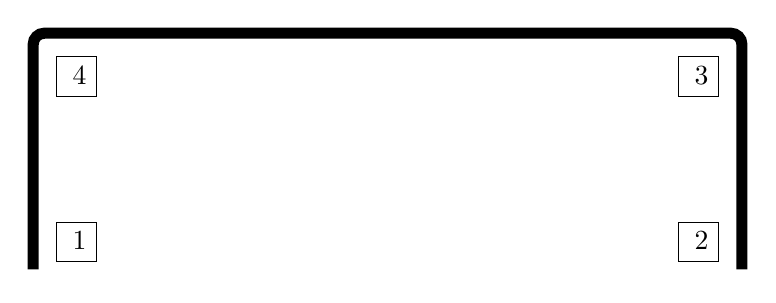
\begin{tikzpicture}[>=stealth]
			\draw[line width =4pt, rounded corners] (0,0)--(0,3)--(9,3)--(9,0);
			\draw (0.3,0.1) rectangle (0.8,0.6) node[below left]{$1$};
			\draw (0.3,2.2) rectangle (0.8,2.7) node[below left]{$4$};
			\draw (8.2,0.1) rectangle (8.7,0.6) node[below left]{$2$};
			\draw (8.2,2.2) rectangle (8.7,2.7) node[below left]{$3$};
			
		\end{tikzpicture}
		\hspace*{-5.5cm}
\begin{tikzpicture}[y=0.80pt, x=0.80pt, yscale=-1, xscale=1, inner sep=0pt, outer sep=0pt,scale=0.9]
			\begin{scope}[shift={(0,99.0)},xscale=0.100,yscale=-0.100,fill=black]
				\path[fill] (480,862) .. controls (441,823) and
				(441,787) .. (479,749) .. controls (507,722) and
				(507,720) .. (485,726) .. controls (471,729) and
				(446,723) .. (420,710) .. controls (364,681) and
				(307,661) .. (245,646) .. controls (202,636) and
				(195,631) .. (195,610) .. controls (195,587) and
				(198,585) .. (235,589) .. controls (257,591) and
				(304,603) .. (340,617) .. controls (376,630) and
				(413,644) .. (423,647) .. controls (438,652) and
				(440,643) .. (440,554) -- (440,456) --
				(402,411) .. controls (348,347) and (344,336) ..
				(336,241) .. controls (329,150) and (336,130) ..
				(375,130) .. controls (408,130) and (417,147) ..
				(424,231) .. controls (431,301) and (435,310) ..
				(476,363) .. controls (501,394) and (527,420) ..
				(533,420) .. controls (540,420) and (566,394) ..
				(591,362) .. controls (635,308) and (637,301) ..
				(644,226) .. controls (650,144) and (658,130) ..
				(697,130) .. controls (732,130) and (739,156) ..
				(729,253) .. controls (721,337) and (718,344) ..
				(675,399) -- (630,456) -- (630,554) .. controls
				(630,662) and (629,661) .. (702,624) .. controls
				(740,605) and (849,580) .. (866,587) .. controls
				(874,590) and (880,602) .. (878,613) .. controls
				(876,629) and (862,636) .. (817,647) .. controls
				(785,654) and (725,675) .. (683,695) .. controls
				(641,714) and (600,730) .. (592,730) .. controls
				(579,730) and (579,732) .. (592,748) .. controls
				(618,776) and (622,807) .. (606,839) .. controls
				(588,874) and (585,875) .. (543,885) .. controls
				(515,891) and (506,887) .. (480,862) -- cycle;
			\end{scope}
			
		\end{tikzpicture}
	\end{center}
	\loigiai{
		Gọi $A_i$ là biến cố cầu thủ sút vào vị trí $i$, $B_i$là biến cố thủ môn bay người đến vị trí $i$ ($i=1,2,3,4$). Dễ thấy $\mathrm{P}(A_i)=\mathrm{P}(B_i)=\dfrac{1}{4}$. Gọi $C$ là biến cố cú sút không vào lưới. Ta có
		\begin{align*}
			\mathrm{P}(C)=\mathrm{P}(A_1)\mathrm{P}(B_1)+ \mathrm{P}(A_2)\mathrm{P}(B_2) + \dfrac{1}{2}\mathrm{P}(A_3)\mathrm{P}(B_3)+ \dfrac{1}{2}\mathrm{P}(A_4)\mathrm{P}(B_4)=\dfrac{3}{16}=0{,}1875.
		\end{align*}
	}
\end{ex}

% #1588 | Archive/2024/Update-SP-BG10-11-3/SP-3/BG11-3/data_1C5/Bai-2-Dang-3-Tinhxacsuatbangdinhnghia-Quan-On.tex | mã gốc 1D9H2-4
\begin{vd}[Mức 2]%[BG Toán 11 CT2025, Quan Ón]%[1D9H2-4]
	Đề cương ôn tập học kỳ I môn Lịch sử lớp $ 11 $ có $ 20 $ câu hỏi. Đề thi học kỳ I gồm $ 3 $ câu hỏi trong $ 20 $ câu hỏi đó. Một học sinh chỉ ôn $ 10 $ câu trong đề cương. Giả sử các câu hỏi trong đề cương đều có khả năng được chọn làm câu hỏi thi như nhau. Hãy tính xác suất để có ít nhất $ 2 $ câu hỏi của đề thi học kỳ I nằm trong số $ 10 $ câu hỏi mà học sinh nói trên đã ôn.	
	\loigiai{
		Không gian mẫu $ \Omega $ là tập hợp các cách chọn 	$ 3 $ câu trong đề cương làm đề thi.\\
		Ta có $n(\Omega) = \mathrm{C}^3_{20} = 1140$.\\
		Gọi $ A $ là biến cố \lq\lq Có ít nhất $2$ câu hỏi của đề thi học kỳ I nằm trong số $ 10 $ câu hỏi mà học sinh nói trên đã ôn\rq\rq.\\
		Ta có $ n(A) = \mathrm{C}^2_{10} \cdot \mathrm{C}^1_{10} + \mathrm{C}^3_{10} = 570 $.\\
		Vậy xác suất cần tìm là $ \mathrm{P}(A) = \dfrac{n(A)}{n(\Omega)} = \dfrac{570}{1140} = \dfrac{1}{2} $.
	}		
\end{vd}

% #1589 | Archive/2024/Update-SP-BG10-11-3/SP-3/BG11-3/data_1C5/Bai-2-Dang-3-Tinhxacsuatbangdinhnghia-Quan-On.tex | mã gốc 1D9H2-4
\begin{vd}[Mức 2]%[BG Toán 11 CT2025, Quan Ón]%[1D9H2-4]
	Trong một hộp đựng $9$ viên bi đỏ và $7$ viên bi xanh. Lấy ngẫu nhiên $4$ viên bi từ hộp trên.
	Xét tính đúng sai của các mệnh đề sau.
	\choiceTF[t]
	{\True Số phần tử của không gian mẫu là $n(\Omega) = \mathrm{C}_{16}^4 = 1820$}
	{Gọi $A$ là biến cố: \lq\lq Lấy được $4$ viên bi cùng màu\rq\rq. Khi đó $n(A) = \mathrm{C}_9^1\cdot \mathrm{C}_7^3  + \mathrm{C}_7^4$}
	{Xác suất để $4$ viên bi được lấy cùng màu là $\dfrac{3}{52}$}
	{\True Xác suất để $4$ viên bi được lấy phải có cả hai màu là $\dfrac{237}{260}$}
	\loigiai{
		\begin{itemchoice}
			\itemch  Vì tổng số bi trong hộp là $9 + 7 = 16$.\\
			Do đó, số phần tử của không gian mẫu là $n(\Omega) = \mathrm{C}_{16}^4 = 1820$.
			\itemch  Ta có $A$ là biến cố: \lq\lq Lấy được $4$ viên bi cùng màu\rq\rq.\\
			Để $4$ viên vi cùng màu thì $4$ viên đều màu đỏ hoặc $4$ viên đều màu xanh.\\
			Do đó $n(A) = \mathrm{C}_9^4 + \mathrm{C}_7^4 = 161$.
			\itemch  Ta có xác suất để $4$ viên bi được lấy cùng màu là
			$$ \mathrm{P}(A) = \dfrac{n(A)}{n(\Omega)} = \dfrac{161}{1820} = \dfrac{23}{260}. $$
			\itemch  Vì $A$ là biến cố: \lq\lq Lấy được $4$ viên bi cùng màu\rq\rq.\\
			Suy ra $\overline{A}$ là biến cố: \lq\lq Lấy được $4$ viên bi khác màu\rq\rq\, hay \lq\lq Lấy được $4$ viên bi có cả hai màu\rq\rq.\\
			Do đó xác suất để $4$ viên bi được lấy phải có cả hai màu là
			$$ \mathrm{P}\left(\overline{A}\right) = 1 - \mathrm{P}(A) = 1 - \dfrac{23}{260} = \dfrac{237}{260}. $$
		\end{itemchoice}
	}
\end{vd}

% #1591 | Archive/2024/Update-SP-BG10-11-3/SP-3/BG11-3/data_1C5/Bai-2-Dang-3-Tinhxacsuatbangdinhnghia-Quan-On.tex | mã gốc 1D9H2-4
\begin{bt}[Mức 2]%[1D9H2-4]
	Gieo một con xúc xắc cân đối đồng chất $ 2 $ lần. Tính xác suất biến cố A: \lq\lq Hai lần xuất hiện mặt có số chấm chấm giống nhau\rq\rq.
	\loigiai{
		Gọi $ \Omega $ là không gian mẫu, suy ra số phần tử không gian mẫu là $ n(\Omega) = 36$.\\
		Ta có $ n(A) = 6 $.\\
		Suy ra xác suất $ \mathrm{P}(A) = \dfrac{n(A)}{n(\Omega)} = \dfrac{1}{6}$.
	}
\end{bt}

% #1592 | Archive/2024/Update-SP-BG10-11-3/SP-3/BG11-3/data_1C5/Bai-2-Dang-3-Tinhxacsuatbangdinhnghia-Quan-On.tex | mã gốc 1D9H2-4
\begin{bt}[Mức 2]%[1D9H2-4]
	Để kiểm tra chất lượng từ một công ty sữa, người ta gửi đến bộ phận kiểm nghiệm $5$ hộp sữa cam, $4$ hộp sữa dâu và $3$ hộp sữa nho. Bộ phận kiểm nghiệm chọn ngẫu nhiên $3$ hộp sữa để phân tích mẫu. Tính xác suất để ba hộp sữa được chọn có cả ba loại.
	\loigiai{
		Chọn ngẫu nhiên 3 hộp sữa trong 12 hộp sữa để phân tích mẫu nên $n(\Omega) = \mathrm{C}_{12}^3 = 220$.\\
		Gọi $A$ là biến cố: \lq\lq Cả ba hộp sữa được chọn có cả ba loại\rq\rq, ta có $n(A) = \mathrm{C}_5^1 \cdot \mathrm{C}_4^1 \cdot \mathrm{C}_3^1 = 60$.\\
		Xác suất để ba hộp sữa được chọn có cả ba loại là $\mathrm{P}(A) = \dfrac{n(A)}{n(\Omega)} = \dfrac{60}{220} = \dfrac{3}{11}$.
	}
\end{bt}

% #1593 | Archive/2024/Update-SP-BG10-11-3/SP-3/BG11-3/data_1C5/Bai-2-Dang-3-Tinhxacsuatbangdinhnghia-Quan-On.tex | mã gốc 1D9H2-4
\begin{bt}[Mức 2]%[1D9H2-4]
	Một tổ có $10$ học sinh trong đó có $4$ học sinh nữ và $6$ học sinh nam. Cần chọn 4 học sinh, tính xác suất sao cho chọn được $4$ học sinh có cả nam và nữ.
	\loigiai{	
		Số cách chọn $4$ học sinh bất kỳ là $\mathrm{C}_{10}^4 = 210$ cách.\\
		Số cách chọn được $4$ học sinh toàn là nam hoặc toàn là nữ là $\mathrm{C}_{4}^4 + \mathrm{C}_{6}^4 = 16$ cách.\\
		Vậy số cách chọn được $4$ học sinh trong đó cả nam và nữ là $210 - 16 = 194$.\\
		Xác suất cần tìm là $\dfrac{194}{210} = \dfrac{97}{105}$.	
	}
\end{bt}

% #1594 | Archive/2024/Update-SP-BG10-11-3/SP-3/BG11-3/data_1C5/Bai-2-Dang-3-Tinhxacsuatbangdinhnghia-Quan-On.tex | mã gốc 1D9H2-4
\begin{bt}[Mức 2]%[1D9H2-4]
	Có $40$ tấm thẻ đánh số thứ tự từ $1$ đến $40$. Chọn ngẫu nhiên ra $10$ tấm thẻ. Tính xác suất để lấy được $5$ tấm thẻ mang số lẻ, $5$ tấm thẻ mang số chẵn trong đó có đúng một thẻ mang số chia hết cho $6$.
	\loigiai{
		Rút ngẫu nhiên $10$ tấm thẻ từ $40$ tấm thẻ có $\mathrm{C}_{40}^{10}$ cách.\\
		Từ số $1$ đến số $40$ có $6$ số chia hết cho $6$ là $6$, $12$, $18$, $24$, $30$, $36$.\\
		Chọn $1$ số chia hết cho $6$ có $6$ cách.\\
		Rút $4$ số chẵn có $\mathrm{C}_{14}^4$ cách.\\
		Rút $5$ số lẻ có $\mathrm{C}_{20}^5$ cách.\\
		Vậy xác suất cần tìm là 
		$ \mathrm{P} = \dfrac{6\cdot\mathrm{C}_{14}^4\cdot\mathrm{C}_{20}^5 }{\mathrm{C}_{40}^{10}} = \dfrac{126}{1147}$.
	}
\end{bt}

% #1595 | Archive/2024/Update-SP-BG10-11-3/SP-3/BG11-3/data_1C5/Bai-2-Dang-3-Tinhxacsuatbangdinhnghia-Quan-On.tex | mã gốc 1D9V2-4
\begin{bt}[Mức 3]%[1D9V2-4]
	Một đoàn tàu có $6$ toa ở sân ga. Có $6$ hành khách từ sân ga lên tàu, mỗi người độc lập với nhau và chọn một toa một cách ngẫu nhiên. Tính xác suất để một toa có $1$ người lên, một toa có $2$ người lên, một toa có $3$ người lên và ba toa không có người nào lên.
	\loigiai{
		Do mỗi người độc lập và có $6$ cách chọn toa tàu để lên nên kích thước của không gian mẫu là $	|\Omega| = 6^6$.\\
		Ta chia ra ba bước để xếp $6$ người vào $6$ toa thoả mãn yêu cầu bài toán như sau
		\begin{itemize}
			\item Chọn $1$ toa làm toa $1$ người và chọn người để ngồi toa đó có $6\cdot 6 = 36$ cách;
			\item Chọn $1$ toa làm toa $2$ người trong $5$ toa còn lại và chọn $2$ người trong $5$ người còn lại có $5\cdot \mathrm{C}^2_5 = 50$ cách;
			\item Chọn $1$ toa cho $3$ người còn lại trong $4$ toa còn lại có $4$ cách.
		\end{itemize}
		Do đó số cách xếp $6$ người vào $6$ toa thoả mãn bài ra là $36\cdot 50 \cdot 4 = 7200$ cách.\\
		Vậy xác suất cần tìm là $\dfrac{7200}{6^6} = \dfrac{25}{162}$.
	}
\end{bt}

% #1596 | Archive/2024/Update-SP-BG10-11-3/SP-3/BG11-3/data_1C5/Bai-2-Dang-3-Tinhxacsuatbangdinhnghia-Quan-On.tex | mã gốc 1D9H2-3
\begin{ex}[Mức 2]%[BG Toán 11 CT2025, Quan Ón]%[1D9H2-3]
	Một hộp đựng $10$ bi, trong đó có $4$ bi xanh và $6$ bi đỏ. Lấy ra $1$ bi và không hoàn lại, tiếp tục lấy ra $1$ bi nữa. Gọi $A$: \lq \lq Bi lấy được lần $1$ màu xanh\rq \rq, $B$: \lq \lq Bi lấy được lần $2$ màu đỏ\rq \rq. Trong các khẳng định sau đây, khẳng định nào đúng, khẳng định nào sai?
	\choiceTF[t]
	{Số phần tử của không gian mẫu là $n(\Omega) = \mathrm{C}_{10}^{2}$}
	{$A$, $B$ là hai biến cố xung khắc}
	{\True Xác suất để bi lấy được lần $1$ màu xanh và bi lấy được lần $2$ màu đỏ là $\dfrac{4}{15}$}
	{\True Xác suất để $2$ bi lấy được cùng màu là $\dfrac{7}{15}$}
	\loigiai{
		\begin{itemchoice}
			\itemch  Ta có $n(\Omega) = 10\cdot 9 = 90$.
			\itemch  Vì (xanh, đỏ) là kết quả thuận lợi của cả hai biến cố $A$ và $B$, tức là $A$, $B$ có thể cùng đồng thời xảy ra nên $A$, $B$ không phải hai biến cố xung khắc.
			\itemch  Số cách bi lấy được lần $1$ màu xanh và bi lấy được lần $2$ màu đỏ là $4\cdot 6 = 24$ cách.\\
			Do đó xác suất để bi lấy được lần $1$ màu xanh và bi lấy được lần $2$ màu đỏ là $\dfrac{24}{90} = \dfrac{4}{15}$.
			\itemch  Số cách để $2$ bi lấy được cùng màu là $4\cdot 3 + 6\cdot 5 = 42$ cách.\\
			Do đó xác suất để $2$ bi lấy được cùng màu là $\dfrac{42}{90} = \dfrac{7}{15}$.
		\end{itemchoice}
	}
\end{ex}

% #1599 | Archive/2024/Update-SP-BG10-11-3/SP-3/BG11-3/data_1C5/Bai-2-Dang-3-Tinhxacsuatbangdinhnghia-Quan-On.tex | mã gốc 1D9V2-3
\begin{ex}[Mức 3]%[BG Toán 11 CT2025, Quan Ón]%[1D9V2-3]
	Một hộp có $18$ viên bi, trong đó có $7$ viên bi màu đỏ được đánh số từ $1$ đến $7$, $6$ viên bi màu xanh được đánh số từ $1$ đến $6$ và $5$ viên bi màu vàng được đánh số từ $1$ đến $5$. Lấy ngẫu nhiên trong hộp ra $3$ viên bi.
	\choiceTF[t]
	{\True Xác suất để lấy được $3$ viên bi màu đỏ là $\dfrac{35}{816}$}
	{Xác suất để lấy được $3$ viên bi cùng màu là $\dfrac{67}{816}$}
	{\True Xác suất để lấy được $3$ viên bi đủ cả ba màu là $\dfrac{35}{136}$}
	{Xác suất để lấy được $3$ viên bi khác màu và khác số là $\dfrac{121}{816}$}
	\loigiai{
		Lấy ngẫu nhiên trong hộp ra $3$ viên bi từ $18$ viên bi nên có $n(\Omega)=\mathrm{C}_{18}^3$.
		\begin{itemchoice}
			\itemch  Gọi $A$ là biến cố \lq\lq Lấy được $3$ viên bi màu đỏ\rq\rq.\\
			Ta có $n(A)=\mathrm{C}_7^3$.\\
			Nên xác suất để lấy được $3$ viên bi màu đỏ là $\mathrm{P}(A) = \dfrac{n(A)}{n(\Omega)}=\dfrac{\mathrm{C}_7^3}{\mathrm{C}_{18}^3}=\dfrac{35}{816}$.
			\itemch  Gọi $B$ là biến cố \lq\lq Lấy được $3$ viên bi cùng màu\rq\rq.\\
			Ta có $\mathrm{P}(B)=\dfrac{\mathrm{C}_7^3+\mathrm{C}_6^3+\mathrm{C}_5^3}{\mathrm{C}_{18}^3}=\dfrac{65}{816}$.
			\itemch  Gọi $C$ là biến cố \lq\lq Lấy được $3$ viên bi đủ cả ba màu\rq\rq. \\
			Vì mỗi màu có $1$ viên nên ta có xác suất xảy ra biến cố $C$ là $\mathrm{P}(C)=\dfrac{\mathrm{C}_7^1 \cdot \mathrm{C}_6^1 \cdot \mathrm{C}_5^1}{\mathrm{C}_{18}^3}=\dfrac{210}{816}=\dfrac{35}{136}$.
			\itemch  Gọi $D$ là biến cố \lq\lq Lấy được $3$ viên bi khác màu và khác số\rq\rq. \\
			Khi đó xác suất xảy ra biến cố $D$ là $\mathrm{P}(D)=\dfrac{5\cdot5\cdot5}{\mathrm{C}_{18}^3}=\dfrac{125}{816}$.
		\end{itemchoice}
	}
\end{ex}

% #1600 | Archive/2024/Update-SP-BG10-11-3/SP-3/BG11-3/data_1C5/Bai-2-Dang-3-Tinhxacsuatbangdinhnghia-Quan-On.tex | mã gốc 1D9V2-3
\begin{ex}[Mức 3]%[BG Toán 11 CT2025, Quan Ón]%[1D9V2-3]
	Lớp 10A1 có $35$ học sinh gồm $20$ học sinh nữ và $15$ học sinh nam. Nhà trường cần chọn $3$ học sinh của lớp đó tham gia trồng cây. Các khẳng định sau đây, khẳng định nào là đúng, khẳng định nào là sai?
	\choiceTF[t]
	{\True Xác suất để $3$ học sinh được chọn có đúng một học sinh nữ bằng $\dfrac{60}{187}$}
	{\True Xác suất để $3$ học sinh được chọn có đúng hai học sinh nữ bằng $\dfrac{570}{1309}$}
	{Xác suất để $3$ học sinh được chọn có ít nhất một học sinh nữ bằng $\dfrac{90}{119}$}
	{Xác suất để $3$ học sinh được chọn có nhiều nhất hai học sinh nữ bằng $\dfrac{114}{187}$}
	\loigiai{
		Ta có số phần tử không gian mẫu $n(\Omega) = \mathrm{C}_{35}^3$.
		\begin{itemchoice}
			\itemch  Gọi $A$: \lq \lq $3$ học sinh được chọn đúng một học sinh nữ\rq \rq.\\
			Ta có $n(A) = 20 \cdot \mathrm{C}_{15}^2$.\\
			Xác suất của biến cố $A$ là $\mathrm{P}(A)=\dfrac{n(A)}{n(\Omega)}=\dfrac{20 \cdot \mathrm{C}_{15}^2}{\mathrm{C}_{35}^3}=\dfrac{60}{187}$.
			\itemch  Gọi $B$: \lq \lq $3$ học sinh được chọn đúng hai học sinh nữ\rq \rq. \\
			Ta có $n(B)=\mathrm{C}_{20}^2 \cdot 15$.\\
			Xác suất của biến cố $B$ là $\mathrm{P}(B)=\dfrac{n(A)}{n(\Omega)}=\dfrac{\mathrm{C}_{20}^2 \cdot 15}{\mathrm{C}_{35}^3}=\dfrac{570}{1309}$.
			\itemch  Gọi $C$: \lq \lq $3$ học sinh được chọn có ít nhất một học sinh nữ\rq \rq.\\
			Ta có  $n(C)=20\cdot \mathrm{C}_{15}^2+\mathrm{C}_{20}^2 \cdot 15 +\mathrm{C}_{20}^3$.\\
			Xác suất của biến cố $C$ là $\mathrm{P}(C)=\dfrac{n(C)}{n(\Omega)}=\dfrac{20\cdot \mathrm{C}_{15}^2+\mathrm{C}_{20}^2 \cdot 15 +\mathrm{C}_{20}^3}{\mathrm{C}_{35}^3}=\dfrac{174}{187}$.
			\itemch  Gọi $D$: \lq \lq $3$ học sinh được chọn có nhiều nhất hai học sinh nữ\rq \rq.\\
			Ta có $n(D)=\mathrm{C}_{15}^3+20\cdot \mathrm{C}_{15}^2+\mathrm{C}_{20}^2 \cdot 15$.\\
			Xác suất của biến cố $D$ là $\mathrm{P}(D)=\dfrac{n(D)}{n(\Omega)}=\dfrac{\mathrm{C}_{15}^3+20\cdot \mathrm{C}_{15}^2+\mathrm{C}_{20}^2 \cdot 15}{\mathrm{C}_{35}^3}=\dfrac{1081}{1309}$.
		\end{itemchoice}
	}
\end{ex}

% #1601 | Archive/2024/Update-SP-BG10-11-3/SP-3/BG11-3/data_1C5/Bai-2-Dang-3-Tinhxacsuatbangdinhnghia-Quan-On.tex | mã gốc 1D9V2-3
\begin{ex}[Mức 3]%[BG Toán 11 CT2025, Quan Ón]%[1D9V2-3]
	Một đội tình nguyện gồm $6$ học sinh khối $10$, $5$ học sinh khối $11$ và $4$ học sinh khối $12$. Chọn ngẫu nhiên $5$ học sinh trong đội. Các khẳng định sau đây, khẳng định nào đúng, khẳng định nào sai?
	\choiceTF[t]
	{Số phần tử không gian mẫu là $15$ phần tử}
	{\True Số phần tử của biến cố \lq\lq Cả $5$ học sinh được chọn học cùng một khối\rq \rq \, là $\mathrm{C}_ 6^5+\mathrm{C}_ 5^5$ phần tử}
	{Xác suất của biến cố \lq\lq Cả $5$ học sinh được chọn học cùng một khối\rq \rq \, là $\dfrac{5}{3003}$}
	{\True Xác suất của biến cố \lq\lq Chọn được $5$ học sinh đủ ba khối\rq \rq \, là $\dfrac{310}{429}$}
	\loigiai{
		Số cách chọn $5$ học sinh trong $15$ học sinh là $\mathrm{C}_{15}^5=3003$ cách.
		\begin{itemchoice}
			\itemch  Số phần tử không gian mẫu là $n(\Omega)=\mathrm{C}_{15}^5=3003$.
			\itemch  Gọi $A$ là biến cố \lq\lq Cả $5$ học sinh được chọn học cùng một khối\rq \rq.\\
			Vì cả $5$ học sinh được chọn học cùng một khối nên chỉ có thể chọn $5$ học sinh khối $10$ hoặc $5$ học sinh khối $11$. Suy ra $n(A)=\mathrm{C}_6^5+\mathrm{C}_5^5$.
			\itemch  Xác suất của biến cố \lq\lq Cả $5$ học sinh được chọn học cùng một khối\rq \rq \ là
			$$\mathrm{P}(A)=\dfrac{n(A)}{n(\Omega)}=\dfrac{\mathrm{C}_6^5+\mathrm{C}_5^5}{\mathrm{C}_{15}^5}=\dfrac{1}{429}.$$
			\itemch  Gọi $B$ là biến cố \lq\lq Chọn được $5$ học sinh đủ ba khối\rq \rq. Khi đó\\
			$n(B)=\mathrm{C}_6^1\cdot \mathrm{C}_5^1\cdot \mathrm{C}_4^3 + \mathrm{C}_6^1\cdot \mathrm{C}_5^3\cdot \mathrm{C}_4^1 + \mathrm{C}_6^1\cdot \mathrm{C}_5^2\cdot \mathrm{C}_4^2 + \mathrm{C}_6^2\cdot \mathrm{C}_5^1\cdot \mathrm{C}_4^2 + \mathrm{C}_6^2\cdot \mathrm{C}_5^2\cdot \mathrm{C}_4^1 + \mathrm{C}_6^3\cdot \mathrm{C}_5^1\cdot \mathrm{C}_4^1 = 2170$.\\
			Vậy $\mathrm{P}(B) = \dfrac{n(B)}{n(\Omega)} = \dfrac{2170}{3003} = \dfrac{310}{429}$.
		\end{itemchoice}
	}
\end{ex}

% #1602 | Archive/2024/Update-SP-BG10-11-3/SP-3/BG11-3/data_1C5/Bai-2-Dang-3-Tinhxacsuatbangdinhnghia-Quan-On.tex | mã gốc 1D9H2-3
\begin{ex}[Mức 2]%[BG Toán 11 CT2025, Quan Ón]%[1D9H2-3]
	Một hộp chứa $15$ quả cầu gồm $6$ quả màu đỏ được đánh số từ $1$ đến $6$ và $9$ quả màu xanh được đánh số từ $1$ đến $9$. Lấy ngẫu nhiên hai quả từ hộp đó, tính xác suất để lấy được hai quả khác màu đồng thời tổng hai số ghi trên chúng là số chẵn (kết quả làm tròn đến hàng phần trăm).
	\shortans{$0{,}26$}
	\loigiai{
		Số cách lấy ngẫu nhiên $2$ quả cầu từ hộp là $\mathrm{C}_{15}^{2} = 105$ cách.\\
		Để tổng hai số ghi trên hai quả cầu là số chẵn ta có $2$ trường hợp sau
		\begin{itemize}
			\item Hai quả cầu khác màu cùng đánh số lẻ: $\mathrm{C}_{3}^{1}\cdot \mathrm{C}_{5}^{1} = 15$ cách.
			\item Hai quả cầu khác màu nhau cùng đánh số chẵn: $\mathrm{C}_{3}^{1}\cdot \mathrm{C}_{4}^{1} = 12$ cách.
		\end{itemize}
		Vậy xác suất cần tính là $\mathrm{P} = \dfrac{15 + 12}{105} = \dfrac{9}{35} \approx 0{,}26$.
	}
\end{ex}

% #1603 | Archive/2024/Update-SP-BG10-11-3/SP-3/BG11-3/data_1C5/Bai-2-Dang-3-Tinhxacsuatbangdinhnghia-Quan-On.tex | mã gốc 1D9V2-3
\begin{ex}[Mức 3]%[BG Toán 11 CT2025, Quan Ón]%[1D9V2-3]
	Một hộp đựng $15$ tấm thẻ được đánh số từ $1$ đến $15$. Chọn ngẫu nhiên $6$ tấm thẻ trong hộp. Tính xác suất để tổng các số ghi trên $6$ tấm thẻ được chọn là một số lẻ (kết quả làm tròn đến hàng phần trăm).
	\shortans{$0{,}50$}
	\loigiai{
		Chọn $6$ tấm thẻ trong hộp có $15$ ta có $\mathrm{C}_{15}^{6} = 5005$ cách\\
		$\Rightarrow n(\Omega) = 5005$ cách.\\
		Ta thấy trong $15$ tấm thẻ có $8$ tấm thẻ đánh số lẻ và $7$ tấm thẻ đánh số
		chẵn.\\
		Gọi A là biến cố: \lq\lq Tổng các số ghi trên 6 tấm thẻ là số lẻ\rq\rq. \\
		Ta có các trường hợp sau
		\begin{itemize}
			\item TH 1: Chọn được $5$ thẻ đánh số lẻ và $1$ thẻ đánh số chẵn có $\mathrm{C}_{8}^{5}\cdot \mathrm{C}_{7}^{1} = 392$ cách.
			\item TH 2: Chọn được $3$ thẻ đánh số lẻ và $3$ thẻ đánh số chẵn có $\mathrm{C}_{8}^{3}\cdot \mathrm{C}_{7}^{3} = 1960$ cách.
			\item TH 3: Chọn được $1$ thẻ đánh số lẻ và $5$ thẻ đánh số chẵn có $\mathrm{C}_{8}^{1}\cdot \mathrm{C}_{7}^{5} = 168$ cách.
		\end{itemize}
		Do đó $n(A) = 392 + 1960 + 168 = 2520$ cách.\\
		Vậy xác suất cần tìm là $\mathrm{P}(A) = \dfrac{n(A)}{n(\Omega)} = \dfrac{2520}{5005} = \dfrac{72}{143} \approx 0{,}50$.
	}
\end{ex}

% #1604 | Archive/2024/Update-SP-BG10-11-3/SP-3/BG11-3/data_1C5/Bai-2-Dang-3-Tinhxacsuatbangdinhnghia-Quan-On.tex | mã gốc 1D9V2-4
\begin{ex}[Mức 3]%[1D9V2-4]
	Xếp $6$ học sinh nam và $4$ học sinh nữ vào một bàn tròn có $10$ ghế. Tính xác suất để không có hai học sinh nữ ngồi cạnh nhau (kết quả làm tròn đến hàng phần trăm).
	\shortans{$0{,}12$}
	\loigiai{
		Cố định $1$ vị trí cho một học sinh nam (hoặc nữ), đánh dấu các ghế còn lại từ $1$ đến $9$.\\
		Không gian mẫu là hoán vị của $9$ học sinh (còn lại, không cố định) trên $9$ ghế đánh dấu.\\
		Suy ra số phần tử không gian mẫu là $n(\Omega)=9!$.\\
		Gọi $A$ là biến cố \lq\lq Không có hai học sinh nữ ngồi cạnh nhau\rq\rq.\\
		Ta mô tả khả năng thuận lợi của biến cố $A$ như sau
		\begin{itemize}
			\item Đầu tiên, ta cố định một học sinh nam, $5$ học sinh còn lại có $5!$ cách sắp xếp.
			\item Sau đó, sắp $4$ bạn nữ vào $4$ trong $6$ khoảng trống giữa hai bạn nam có $\mathrm{A}_6^4$ cách.
		\end{itemize}
		Suy ra số phần tử của biến cố $A$ là $n(A) = 5!\cdot \mathrm{A}_6^4$.\\
		Vậy $P(A) = \dfrac{n(A)}{n(\Omega)} = \dfrac{5!\cdot \mathrm{A}_6^4}{9!} = \dfrac{5}{42} \approx 0{,}12$.
	}
\end{ex}

% #1605 | Archive/2024/Update-SP-BG10-11-3/SP-3/BG11-3/data_1C5/Bai-2-Dang-3-Tinhxacsuatbangdinhnghia-Quan-On.tex | mã gốc 1D9V2-4
\begin{ex}[Mức 3]%[1D9V2-4]
	Cho đa giác đều $(P)$ có $20$ đỉnh. Lấy tùy ý $3$ đỉnh  của $(P)$, xác suất để $3$ đỉnh lấy được tạo thành tam giác vuông không có cạnh nào là cạnh của $(P)$ có dạng $\dfrac{a}{b}$ với $\dfrac{a}{b}$ tối giản. Tính giá trị của biểu thức $T = b - a$. 
	\shortans{$50$}
	\loigiai{
		Số tam giác tạo thành từ $20$ đỉnh là $\mathrm{C}_{20}^3$, suy ra $n(\Omega) = \mathrm{C}_{20}^3 = 1140$.\\
		Gọi $A$ là biến cố: \lq\lq$3$ đỉnh lấy được tạo thành tam giác vuông không có cạnh nào là cạnh của $(P)$\rq\rq.\\
		Số đường chéo của đa giác đều là $10$. Mỗi đường chéo là cạnh huyền của tam giác vuông có đỉnh thứ ba là các đỉnh còn lại khác hai đỉnh của đường chéo.\\
		Số tam giác vuông là $18\cdot 10 = 180$.\\
		Số tam giác vuông có một cạnh là cạnh của đa giác là $4\cdot 10 = 40$.\\
		Suy ra số tam giác vuông tạo từ $20$ đỉnh của đa giác đều mà không có cạnh nào là cạnh của đa giác là $n(A) = 180 - 40 = 140$.\\
		Do đó $\mathrm{P}(A) = \dfrac{n(A)}{n(\Omega)} = \dfrac{140}{1140} = \dfrac{7}{57}$.\\
		Suy ra $a = 7$ và $b = 57$.\\
		Vậy $T = b - a = 57 - 7 = 50$.
	}
\end{ex}

% #1606 | Archive/2024/Update-SP-BG10-11-3/SP-3/BG11-3/data_1C5/Bai-2-Dang-3-Tinhxacsuatbangdinhnghia-Quan-On.tex | mã gốc 1D9V2-4
\begin{ex}[Mức 3]%[1D9V2-4]
	Gọi $S$ là tập hợp các số tự nhiên có $4$ chữ số khác nhau. Chọn ngẫu nhiên một số từ tập $S$. Khi đó, xác suất để số được chọn có các chữ số sắp xếp theo thứ tự tăng dần và không chứa hai chữ số nguyên nào liên tiếp nhau có dạng $\dfrac{a}{b}$ với $\dfrac{a}{b}$ tối giản. Tính giá trị biểu thức $T = b - 100a - 12$.
	\shortans{$1000$}
	\loigiai{
		Xét phép thử \lq\lq Chọn ngẫu nhiên một số từ tập $S$\rq\rq.\\
		Số phần tử của không gian mẫu là $n\left( \Omega \right) = 9 \cdot \mathrm{A}_9^3 = 4536$.\\
		Gọi $A$ là biến cố: \lq\lq Số được chọn có các chữ số sắp xếp theo thứ tự tăng dần và không chứa hai chữ số nguyên nào liên tiếp nhau\rq\rq.\\
		Gọi số được chọn là $\overline{abcd}$.\\
		Khi đó
		\begin{itemize}
			\item Vì chữ số sắp xếp theo thứ tự tăng dần nên $1 \leq a < b < c < d \leq 9$.
			\item Trong số được chọn không chứa hai chữ số nguyên nào liên tiếp nhau nên: $1 \leq a < b-1 < c-2 < d-3 \leq 6$.
		\end{itemize}
		Đặt $a_1 = a$; $b_1 = b-1$; $c_1 = c-2$; $d_1 = d-3$. Khi đó $1 \leq a_1 < b_1 < c_1 < d_1 \leq 6$.\\
		Số cách chọn bộ bốn số $(a_1;b_1;c_1;d_1)$ là $\mathrm{C}_6^4$ (cách) $\Rightarrow$ có $\mathrm{C}_6^4$ cách chọn $a$; $b$; $c$; $d$.\\
		Mỗi cách chọn $(a;b;c;d)$ chỉ có một cách sắp xếp thỏa mãn yêu cầu bài toán nên tạo ra một số. \\
		Suy ra $n(A) = \mathrm{C}_6^4 = 15$.\\
		Xác suất cần tìm là $\mathrm{P}(A) = \dfrac{n(A)}{n\left( \Omega \right)} = \dfrac{5}{1512}$.\\
		Do đó $a = 5$ và $b = 1512 \Rightarrow T = b - 100a - 12 = 1512 - 100\cdot 5 - 12 = 1000$.
	}
\end{ex}

% #1607 | Archive/2024/Update-SP-BG10-11-3/SP-3/BG11-3/data_1C5/DS11-C5-B2-Dang5-TinhXacSuatBangQuyTacNhan-TranTony.tex | mã gốc 1D9H1-3
\begin{vd}%[Bài giảng 11, Trần Tony]%[1D9H1-3]
	Gieo đồng thời một đồng xu và một con súc sắc. Xác suất để đồng xu xuất hiện mặt sấp là $0{,}5$ và xác suất để con súc sắc xuất hiện mặt chẵn chấm là $0{,}5$. Tính xác suất để đồng xu xuất hiện mặt ngửa và con súc sắc xuất hiện mặt chẵn chấm.
	\loigiai{
		Vì xác suất đồng xu xuất hiện mặt sấp là $0{,}5$ nên xác suất để đồng xu xuất hiện mặt ngửa là $\mathrm{P}(A)=0{,}5$.\\
		Gọi $\mathrm{P}(B)=0{,}5$ là xác suất để con súc sắc xuất hiện mặt chẵn chấm.\\
		Do xác suất xuất hiện mặt chẵn hoặc lẻ của đồng xu độc lập với sự xuất hiện các mặt của con súc sắc nên ta có $$\mathrm{P}\left(A\cap B\right)=\mathrm{P}(A)\cdot\mathrm{P}(B)=0{,}5\cdot0{,}5=0{,}25.$$
	}
\end{vd}

% #1608 | Archive/2024/Update-SP-BG10-11-3/SP-3/BG11-3/data_1C5/DS11-C5-B2-Dang5-TinhXacSuatBangQuyTacNhan-TranTony.tex | mã gốc 1D9H1-3
\begin{vd}%[Bài giảng 11, Trần Tony]%[1D9H1-3]
	Một xưởng sản suất có hai chiếc máy chạy độc lập với nhau. Xác suất để máy $I$ và $II$ chạy tốt lần lượt là $0{,}7$ và $0{,}8$. Tính xác suất để xưởng có hai máy đều chạy tốt.
	\loigiai{
		Gọi $\mathrm{P}(A)=0{,}7$ là xác suất để máy $I$ chạy tốt và $\mathrm{P}=0{,}8$ là xác suất để máy $II$ chạy tốt.\\
		Vì hai máy là độc lập nhau nên ta có $\mathrm{P}\left(A\cap B\right)=\mathrm{P}(A)\cdot\mathrm{P}(B)=0{,}7\cdot0{,}8=0{,}56$.
	}
\end{vd}

% #1609 | Archive/2024/Update-SP-BG10-11-3/SP-3/BG11-3/data_1C5/DS11-C5-B2-Dang5-TinhXacSuatBangQuyTacNhan-TranTony.tex | mã gốc 1D9H1-3
\begin{vd}%[Bài giảng 11, Trần Tony]%[1D9H1-3]
	Hai vận động viên cùng bắn vào bia, biết xác suất bắn trúng hồng tâm của hai vận động viên $I$ và $II$ lần lượt là $0{,}7$ và $0{,}9$. Tính xác suất để cả hai vận động viên đều bắn trượt hồng tâm của bia.
	\loigiai{
		Gọi $\mathrm{P}(A)=0{,}7$ là xác suất bắn trúng hồng tâm của bia của vận động viên số $I$. Vậy xác suất bắn trượt hồng tâm của bia của vđv $I$ là $\mathrm{P}(\overline{A})=0{,}3$.\\
		Gọi $\mathrm{P}(B)=0{,}9$ là xác suất bắn trúng hồng tâm của bia của vận động viên số $II$. Vậy xác suất bắn trượt hồng tâm của bia của vđv $II$ là $\mathrm{P}(\overline{B})=0{,}1$.\\
		Vì xác suất của hai vận động viên là độc lập với nhau nên để cả hai vận động viên bắn trượt bia là
		$$\mathrm{P}(\overline{A}\cap\overline{B})=0{,}3\cdot0{,}1=0{,}03.$$
	}
\end{vd}

% #1610 | Archive/2024/Update-SP-BG10-11-3/SP-3/BG11-3/data_1C5/DS11-C5-B2-Dang5-TinhXacSuatBangQuyTacNhan-TranTony.tex | mã gốc 1D9V1-3
\begin{vd}%[Bài giảng 11, Trần Tony]%[1D9V1-3]
	Cho ba hộp giống nhau, mỗi hộp $7$ bút chỉ khác nhau về màu sắc.\\
	Hộp thứ nhất: Có $3$ bút màu đỏ, $2$ bút màu xanh, $2$ bút màu đen;\\
	Hộp thứ hai: Có $2$ bút màu đỏ, $2$ màu xanh, $3$ màu đen;\\
	Hộp thứ ba: Có $5$ bút màu đỏ, $1$ bút màu xanh, $1$ bút màu đen.
	\choiceTF[t]
	{\True Lấy ngẫu nhiên một hộp, xác suất lấy được hộp thứ nhất là $\dfrac{1}{3}$}
	{Số cách lấy $2$ bút từ $7$ bút là $\mathrm{A}_7^2$}
	{Rút từ hộp thứ nhất ra $2$ bút, xác suất của biến cố "rút được hai bút ở hộp thứ nhất không có màu đen" là $\dfrac{10}{63}$}
	{\True Lấy ngẫu nhiên một hộp, rút từ hộp đó ra $2$ bút. Xác suất của biến cố “Lấy được hai bút không có màu đen” là $\dfrac{31}{63}$}
	\loigiai{		
		\begin{itemchoice}
			\itemch  Xác suất lấy được hộp thứ nhất là $\dfrac{1}{3}$.
			\itemch  Số cách lấy $2$ bút từ $7$ bút là $\mathrm{C}_7^2$.
			\itemch  Xác suất của biến cố "rút được hai bút ở hộp thứ nhất không có màu đen" là $\dfrac{\mathrm{C}_5^2}{\mathrm{C}_7^2}=\dfrac{10}{21}$
			\itemch 
			Gọi $A_i$ là biến cố rút hai bút ở hộp thứ $i$ không có màu đen.\\
			Ta thấy các biến cố $A_1$; $A_2$; $A_3$ đôi một xung khắc với nhau.\\
			Xác suất lấy được hộp thứ $1$ là $\dfrac{1}{3}$.\\
			Tương tự; xác suất để lấy được hộp thứ $2$; thứ $3$ cũng là $\dfrac{1}{3}$.\\
			Ta có $P(A_1)=\dfrac{\mathrm{C}_5^2}{\mathrm{C}_7^2}$, $P(A_2)=\dfrac{\mathrm{C}_4^2}{\mathrm{C}_7^2}$, $P(A_3)=\dfrac{\mathrm{C}_6^2}{\mathrm{C}_7^2}$.\\
			Xác suất cần tính $P=\dfrac{1}{3}P(A_1)+\dfrac{1}{3}P(A_2)+\dfrac{1}{3}P(A_3)=\dfrac{31}{63}$.
		\end{itemchoice}
	}
\end{vd}

% #1612 | Archive/2024/Update-SP-BG10-11-3/SP-3/BG11-3/data_1C5/DS11-C5-B2-Dang5-TinhXacSuatBangQuyTacNhan-TranTony.tex | mã gốc 1D9H1-3
\begin{bt}%[Bài giảng 11, Trần Tony]%[1D9H1-3]
	Hai đội bóng $A$ và $B$ nằm ở hai bảng đấu khác nhau của một giải đấu bóng đá. Biết rằng xác suất để hai đội vào vòng chung kết lần lượt là $0{,}26$ và $0{,}34$. Biết rằng mỗi bảng đấu chỉ có một đội lọt vào vòng chung kết. Tính xác suất để hai đội $A$ và $B$ đều lọt vào vòng chung kết.
	\loigiai{
		Gọi xác suất của đội $A$ và $B$ vào chung kết lần lượt là $\mathrm{P}(A)=0{,}26$, $\mathrm{P}(B)=0{,}34$.\\
		Xác suất để cả hai đội đều lọt vào chung kết là $\mathrm{P}(A\cap B)=0{,}26\cdot 0{,}34=0{,}0884=8{,}84\%$.
	}
\end{bt}

% #1613 | Archive/2024/Update-SP-BG10-11-3/SP-3/BG11-3/data_1C5/DS11-C5-B2-Dang5-TinhXacSuatBangQuyTacNhan-TranTony.tex | mã gốc 1D9H1-3
\begin{bt}%[Bài giảng 11, Trần Tony]%[1D9H1-3]
	Một đề kiểm tra $5$ phút có hai câu trắc nghiệm. Biết xác suất đúng mỗi câu là $0{,}25$. Tính xác suất để một học sinh không học bài có thể khoang đúng được cả hai câu.
	\loigiai{
		Gọi xác suất để học sinh khoanh đúng hai câu hỏi lần lượt là $\mathrm{P}(A)=\mathrm{P}(B)=0{,}25$.\\
		Vì mỗi biến cố là độc lập với nhau nên ta có xác suất cần tìm là $\mathrm{P}(A\cap B)=0{,}25\cdot 0{,}25=0{,}0625$.
	}
\end{bt}

% #1614 | Archive/2024/Update-SP-BG10-11-3/SP-3/BG11-3/data_1C5/DS11-C5-B2-Dang5-TinhXacSuatBangQuyTacNhan-TranTony.tex | mã gốc 1D9H1-3
\begin{bt}%[Bài giảng 11, Trần Tony]%[1D9H1-3]
	Hai đội công nhân trong một nhà máy sản xuất có xác suất tạo ra sản phẩm tốt lần lượt là $0{,}75$ và $0{,}85$. Tính xác suất phế phẩm mà nhà máy đó tạo ra bởi cả hai đội.
	\loigiai{
		Gọi xác suất tạo ra sản phẩm tốt của hai đội công nhân lần lượt là $\mathrm{P}(A)=0{,}75$ và $\mathrm{P}(B)=0{,}85$.\\
		Gọi xác suất tạo ra phế phẩm của hai đội công nhân lần lượt là $\mathrm{P}(\overline{A})=0{,}25$ và $\mathrm{P}(\overline{B})=0{,}15$.\\
		Vậy xác suất phế phẩm mà nhà máy đó tạo ra bỏi cả hai đội là
		$$\mathrm{P}\left(\overline{A}\cap \overline{B}\right)=0{,}25\cdot 0{,}15=0{,}0375.$$
	}
\end{bt}

% #1615 | Archive/2024/Update-SP-BG10-11-3/SP-3/BG11-3/data_1C5/DS11-C5-B2-Dang5-TinhXacSuatBangQuyTacNhan-TranTony.tex | mã gốc 1D9H1-3
\begin{bt}%[Bài giảng 11, Trần Tony]%[1D9H1-3]
	Hai bạn An và Minh cùng tham gia giải cờ vua cấp tỉnh. Biết rằng hai bạn không ở chung $1$ bảng và mỗi bảng chỉ có một người vô vòng chung kết. Biết xác suất vô vòng chung kết của An và Minh lần lượt là $0{,}35$ và $0{,}45$. Tính xác suất để An và Minh cùng vô vòng chung kết.
	\loigiai{
		Gọi xác suất để An và Minh vô vòng chung kết lần lượt là $\mathrm{P}(A)=0{,}35$ và $\mathrm{P}(B)=0{,}45$.\\
		Vậy xác suất để cả hai bạn cùng vô vòng chung kết là $\mathrm{P}(A\cap B)=0{,}35\cdot 0{,}45=0{,}1575$.
	}
\end{bt}

% #1616 | Archive/2024/Update-SP-BG10-11-3/SP-3/BG11-3/data_1C5/DS11-C5-B2-Dang5-TinhXacSuatBangQuyTacNhan-TranTony.tex | mã gốc 1D9H1-3
\begin{bt}%[Bài giảng 11, Trần Tony]%[1D9H1-3]
	Một nhà máy có hai tổ máy sản xuất một mặt hàng, biết rằng xác suất để hai tổ máy phải nghỉ để bảo dưỡng lần lượt là $0{,}2$ và $0{,}32$. Tính xác suất để cả hai tổ máy đều hoạt động.
	\loigiai{
		Gọi xác suất để hai tổ máy phải nghỉ để bảo dưỡng lần lượt là $\mathrm{P}(A)=0{,}2$ và $\mathrm{P}(B)=0{,}32$.\\
		Nên xác suất để hai tổ máy đều hoạt động là $\mathrm{\overline{A}}=0{,}8$ và $\mathrm{\overline{B}}=0{,}68$.\\
		Vậy xác suất để cả hai tổ máy đều hoạt động là $\mathrm{P}\left(\overline{A}\cap \overline{B}\right)=0{,}8\cdot 0{,}68=0{,}544$.
	}
\end{bt}

% #1618 | Archive/2024/Update-SP-BG10-11-3/SP-3/BG11-3/data_1C5/DS11-C5-B2-Dang5-TinhXacSuatBangQuyTacNhan-TranTony.tex | mã gốc 1D9V1-3
\begin{ex}%[Bài giảng 11, Trần Tony]%[1D9V1-3]
	Hai bạn An và Hà của lớp 11A tham gia giải bóng bàn đơn nữ do nhà trường tổ chức. Hai bạn đó nằm ở hai bảng đấu loại khác nhau, mỗi bảng đấu loại chỉ chọn một người vào vòng chung kết. Xác suất lọt qua vòng loại để vào vòng chung kết của An và Hà lần lượt là $0{,}6$ và $0{,}7$.
	\choiceTF[t]
	{\True Biến cố "Bạn An lọt vào vòng chung kết" và biến cố "Bạn Hà lọt vào vòng chung kết" là hai biến cố độc lập}
	{\True Xác suất cả hai bạn lọt vào vòng chung kết là $0{,}42$}
	{Xác suất có ít nhất một bạn lọt vào vòng chung kết là $0{,}8$}
	{Xác suất chỉ có bạn Hà lọt vào vòng chung kết là $0{,}7$}
	\loigiai{
		\begin{itemchoice}
			\itemch  Biến cố "Bạn An lọt vào vòng chung kết" và biến cố "Bạn Hà lọt vào vòng chung kết" là hai biến cố độc lập.
			\itemch  Xác suất cả hai bạn lọt vào vòng chung kết là $0{,}6\cdot 0{,}7=0{,}42$.
			\itemch  
			Xác suất không lọt vào vòng chung kết của An là $0{,}4$.\\
			Xác suất không lọt vào vòng chung kết của Hà là $0{,}3$.\\			
			Xác suất không có bạn nào lọt vào vòng chung kết là $0{,}4\cdot 0{,}3=0{,}12$.\\
			Xác suất có ít nhất một bạn nào lọt vào vòng chung kết là $1-0{,}12=0{,}88$.
			\itemch  Xác suất chỉ có bạn Hà lọt vào vòng chung kết là $0{,}7\cdot 0{,}4=0{,}28$.
		\end{itemchoice}
	}
\end{ex}

% #1620 | Archive/2024/Update-SP-BG10-11-3/SP-3/BG11-3/data_1C5/DS11-C5-B2-Dang5-TinhXacSuatBangQuyTacNhan-TranTony.tex | mã gốc 1D9V1-3
\begin{ex}%[Bài giảng 11, Trần Tony]%[1D9V1-3]
	Có $6$ bạn nam trong đó có Hoàng và $3$ bạn nữ xếp ngẫu nhiên thành một hàng ngang.
	\choiceTF[t]
	{Số cách xếp $9$ bạn thành hàng ngang là $4320$}
	{\True Số cách xếp $9$ bạn thành hàng ngang mà bạn Hoàng đứng ngoài cùng là $80640$}
	{Số cách xếp $9$ bạn thành hàng ngang mà $6$ bạn nam luôn đứng cạnh nhau là $4320$}
	{\True Xác suất để không có hai bạn nữ nào đứng cạnh nhau và Hoàng đứng ở ngoài cùng bằng $\dfrac{5}{63}$}
	\loigiai{
	\begin{itemchoice}
		\itemch  Số cách xếp $9$ bạn thành hàng ngang là $9!=362880$.
		\itemch  Số cách xếp $9$ bạn thành hàng ngang mà bạn Hoàng đứng ngoài cùng là $2\cdot 8!=80640$.
		\itemch  Số cách xếp $9$ bạn thành hàng ngang mà $6$ bạn nam luôn đứng cạnh nhau là $6!\cdot 4!=17280$.
		\itemch 
			\begin{itemize}
				\item Số cách xếp tùy ý $9$ bạn thành hàng ngang là $9!$ $\Rightarrow n(\Omega)=9!$.
				\item Số cách xếp sao cho không có hai bạn nữ nào đứng cạnh nhau và Hoàng đứng ở ngoài cùng
				\begin{itemize}
					\item Xếp $6$ bạn nam thành một hàng ngang sao cho Hoàng đứng ở ngoài cùng, có $2\cdot 5!$ cách.
					\item Xếp 3 bạn nữ vào 6 khoảng trống tạo bởi 6 bạn nam đã được xếp, trừ khoảng trống ngoài cùng bên cạnh Hoàng, có $\mathrm{A}_6^3$ cách.
				\end{itemize}
			\end{itemize}
			Vậy số cách xếp để không có hai bạn nữ nào đứng cạnh nhau và Hoàng đứng ở ngoài cùng bằng: $2\cdot 5 ! \cdot \mathrm{A}_6^3$. Suy ra, xác suất để không có hai bạn nữ nào đứng cạnh nhau và Hoàng đứng ở ngoài cùng bằng $\dfrac{2\cdot 5! \cdot \mathrm{A}_6^3}{n(\Omega)}=\dfrac{2\cdot 5! \cdot  \mathrm{A}_6^3}{9!}=\dfrac{5}{63}$.
	\end{itemchoice}
	}
\end{ex}

% #1622 | Archive/2024/Update-SP-BG10-11-3/SP-3/BG11-3/data_1C5/DS11-C5-B2-Dang5-TinhXacSuatBangQuyTacNhan-TranTony.tex | mã gốc 1D9V1-3
\begin{ex}%[Bài giảng 11, Trần Tony]%[1D9V1-3]
	Trong một trò chơi trên truyền hình có một bộ câu hỏi gồm $6$ câu hỏi trắc nghiệm khách quan. Mỗi câu có $4$ phương án trả lời, trong đó chỉ có một phương án đúng. Một người chơi trả lời bộ câu hỏi bằng cách chọn ngẫu nhiên một phương án trả lời ở mỗi câu hỏi. Tính xác suất để người đó trả lời đúng $3$ câu. 
	\shortans{$0{,}13$}
	\loigiai{
		Gọi $A_i$ là biến cố trả lời đúng câu thứ $i$ với $i=1,2,\ldots,6$. Suy ra $\mathrm{P}(A_i)=\dfrac{1}{4}$, $\mathrm{P}(\overline{A_i})=\dfrac{3}{4}$.\\
		 xác suất để người đó trả lời đúng $3$ câu là $P=\mathrm{C}_6^3\left(\dfrac{1}{4}\right)^3\left(\dfrac{3}{4}\right)^3\approx 0{,}13$.
	}
\end{ex}

% #1623 | Archive/2024/Update-SP-BG10-11-3/SP-3/BG11-3/data_1C5/DS11-C5-B2-Dang5-TinhXacSuatBangQuyTacNhan-TranTony.tex | mã gốc 1D9C1-3
\begin{ex}%[Bài giảng 11, Trần Tony]%[1D9C1-3]
	Có $3$ xạ thủ cùng bắn vào bia với xác suất bắn trúng bia của mỗi xạ thủ lần lượt là $0{,}7$; $0{,}6$ và $0{,}5$. Tính xác suất để có ít nhất $1$ người bắn trúng bia (kết quả làm tròn đến hàng phần trăm).
	\shortans{$0{,}94$}
	\loigiai{
		Gọi $A_1$ là biến cố: ``xạ thủ thứ $1$ bắn trúng'' $\Rightarrow\mathrm{P}(A_1)=0,7$.\\
		Khi đó $\overline{A_1}$ là biến cố: ``xạ thủ thứ nhất bắn không trúng'' $\Rightarrow\mathrm{P}(\overline{A_1})=0{,}3$.\\
		Tương tự: $\mathrm{P}(A_2)=0{,}6$, $\mathrm{P}(\overline{A_2})=0{,}4$, $\mathrm{P}(A_3)=\mathrm{P}(\overline{A_3})=0{,}5$.\\
		Gọi $B$ là biến cố: ``cả $3$ người không bắn trúng bia''.\\
		Khi đó $\overline{B}$ là biến cố: ``có ít nhất $1$ người bắn trúng bia''.\\
		$\mathrm{P}(B)=\mathrm{P}\left(\overline{A_1}\overline{A_2}\overline{A_3}\right)=\mathrm{P}\left(\overline{A_1}\right)\times\mathrm{P}\left(\overline{A_2}\right)\times\mathrm{P}\left(\overline{A_3}\right)=0{,}3\times0{,}4\times0{,}5=0{,}06\\
		\Rightarrow\mathrm{P}\left(\overline{B}\right)=1-0{,}06=0{,}94$.
		}
\end{ex}

% #1624 | Archive/2024/Update-SP-BG10-11-3/SP-3/BG11-3/data_1C5/DS11-C5-B2-Dang5-TinhXacSuatBangQuyTacNhan-TranTony.tex | mã gốc 1D9C1-3
\begin{ex}%[Bài giảng 11, Trần Tony]%[1D9C1-3]
	Một công nhân phải theo dõi và can thiệp hoạt động của hai máy dệt A và B. Trong một giờ, xác suất để máy dệt A hỏng là $\dfrac{1}{7}$; xác suất máy dệt B hỏng là $\dfrac{1}{5}$. Tính xác suất để người công nhân không phải can thiệp máy nào trong một giờ (kết quả làm tròn đến hàng phần trăm).
	\shortans{$0{,}69$}
	\loigiai{
		Gọi $\overline{A}$ là biến cố máy dệt A không bị hỏng trong một giờ.\\
		Gọi $\overline{B}$ là biến cố máy dệt B không bị hỏng trong một giờ.\\
		Xác suất máy dệt A hỏng độc lập với xác suất máy dệt B hỏng.\\
		Ta có: 
		$\mathrm{P}( \overline{A})=1-\mathrm{P}(A)=1-\dfrac{1}{7}=\dfrac{6}{7}$,
		$\mathrm{P}( \overline{B})=1-\mathrm{P}(B)=1-\dfrac{1}{5}=\dfrac{4}{5}$.\\
		Xác suất để người công nhân không phải can thiệp máy nào trong một giờ là\\
		\begin{center}
			$\mathrm{P}( \overline{A}\overline{B}  )=\dfrac{6}{7}\cdot\dfrac{4}{5}=\dfrac{24}{35}\approx 0{,}69$.
		\end{center}
	}
\end{ex}

% #1625 | Archive/2024/Update-SP-BG10-11-3/SP-3/BG11-3/data_1C5/DS11-C5-B2-Dang5-TinhXacSuatBangQuyTacNhan-TranTony.tex | mã gốc 1D9C1-3
\begin{ex}%[Bài giảng 11, Trần Tony]%[1D9C1-3]
	Một bình đựng $9$ viên bi xanh và $7$ viên bi đỏ. Lần lượt lấy ngẫu nhiên ra $2$ bi, mỗi lần lấy $1$ bi. Tính xác suất để bi thứ $2$ màu xanh nếu biết bi thứ nhất màu đỏ (kết quả làm tròn đến hàng phần trăm).
	\shortans{$0{,}26$}
	\loigiai{
		Gọi $A$ là biến cố lần thứ nhất lấy được bi màu đỏ.\\
		Gọi $B$ là biến cố lần thứ hai lấy được bi màu xanh.\\
		Xác suất để lần thứ nhất lấy được bi màu đỏ là: $P(A)= \dfrac{7}{16}$\\
		Xác suất để lần thứ hai lấy được bi màu xanh (trong $15$ viên bi còn lại) là: $P(B)= \dfrac{9}{15}= \dfrac{3}{5}$.\\
		Hai biến cố $A$ và $B$ độc lập với nhau nên áp dụng quy tắc nhân xác suất ta có
		$$P(AB)= P(A)P(B)=\dfrac{7}{16}\cdot \dfrac{3}{5} = \dfrac{21}{80}\approx 0{,}26.$$
	}
\end{ex}

% #1626 | Archive/2024/Update-SP-BG10-11-3/SP-3/BG11-3/data_1C5/DS11-C5-B2-Dang5-TinhXacSuatBangQuyTacNhan-TranTony.tex | mã gốc 1D9C1-3
\begin{ex}%[Bài giảng 11, Trần Tony]%[1D9C1-3]
	Gieo ngẫu nhiên $n$ đồng xu. Tìm $n$ lớn nhất để xác suất tất cả các đồng xu không cùng ngửa hoặc không cùng sấp luôn nhỏ hơn $\dfrac{63}{64}$.
	\shortans{$6$}
	\loigiai{
		Không gian mẫu có $2^n$ phần tử.\\
		Gọi $A$ là biến cố các mặt không cùng sấp hoặc không cùng ngửa. Suy ra $\overline{A}$ có $2$ phần tử là $SS\ldots S$ và $NNN\ldots N $.\\
		Suy ra $P(A)=1-P(\overline{A})=1-\dfrac{2}{2^n}=1-\dfrac{1}{2^{n-1}}$.\\
		$P(A)<\dfrac{63}{64}\Leftrightarrow \dfrac{1}{2^{n-1}}>\dfrac{1}{64}\Leftrightarrow n<7$.\\
		Vậy $n$ lớn nhất là $n=6$.
	}
\end{ex}

% #2420 | Archive/SP_DA_SauLuoi/1-TL-TN-THPT-Nhu-Van-Lan-Hai-Phong-HKII-NH23-24.tex | mã gốc 1D9V1-3
\begin{ex}%[1D9V1-3]%[Dự án đề kiểm tra Toán 11 HKII NH23-24- Thái Bảo]%[THPT Nhữ Văn Lan- Hải Phòng]
	Một lớp học có $40$ học sinh, trong đó có $18$ học sinh tham gia môn bóng đá và $10$ học sinh tham gia môn bóng chuyền, trong đó có $6$ học sinh tham gia cả hai môn bóng đá và bóng chuyền. Thầy giáo chọn ngẫu nhiên một học sinh từ lớp học để làm nhiệm vụ đặc biệt, gọi $A$ là biến cố: "Chọn được một học sinh tham gia môn bóng đá", $B$ là biến cố: "Chọn được một học sinh tham gia môn bóng chuyền". Khi đó các mệnh đề sau đúng hay sai?
	\choiceTF[t]
	{Xác suất để học sinh được chọn có tham gia ít nhất một trong hai môn thể thao bằng $\dfrac{13}{20}$}
	{$\mathrm{P}(AB)=\dfrac{7}{20}$}
	{\True $\mathrm{P}(B)=\dfrac{1}{4}$}
	{\True $\mathrm{P}(A)=\dfrac{9}{20}$}
	\loigiai{
		Ta có
		\begin{itemchoice}
			\itemch Sai. Vì $\mathrm{P}(A\cup B)=\mathrm{P}(A)+\mathrm{P}(B)-\mathrm{P}(AB)=\dfrac{9}{20}+\dfrac{1}{4}-\dfrac{3}{20}=\dfrac{11}{20}$.
			\itemch Sai. Vì $\mathrm{P}(AB)=\dfrac{6}{40}=\dfrac{3}{20}$.
			\itemch Đúng. Vì $\mathrm{P}(B)=\dfrac{10}{40}=\dfrac{1}{4}$.
			\itemch Đúng. Vì $\mathrm{P}(A)=\dfrac{18}{40}=\dfrac{9}{20}$.
		\end{itemchoice}
	}
\end{ex}

% #2422 | Archive/SP_DA_SauLuoi/1-TL-TN-THPT-Nhu-Van-Lan-Hai-Phong-HKII-NH23-24.tex | mã gốc 1D9H2-4
\begin{ex}%[1D9H2-4]]%[Dự án đề kiểm tra Toán 11 HKII NH23-24- Phạm Quốc Toàn]%[THPT Nhữ Văn Lan- Hải Phòng]
Ba người cùng bắn vào một bia. Xác suất bắn trúng đích của người thứ nhất, thứ hai, thứ ba lần lượt là $0,7$; $0,6$; $0,8$. Xác suất để có đúng hai người bắn trúng đích (làm tròn đến hàng phần trăm)?
\shortans[1]{$0{,}45$}
\loigiai
{
Gọi $A_i$ là biến cố \lq\lq Người thứ $i$ bắn trúng đích\rq\rq\, với $i \in \left\{1;2;3\right\}$.\\
Gọi $B$ là biến cố \lq\lq Có đúng hai người bắn trúng bia\rq\rq.\\
Khi đó $B=A_1A_2\overline{A_3}\cup \overline{A_1}A_2A_3\cup A_1\overline{A_2}A_3$.\\
Ta có 
\begin{eqnarray*}
\mathrm{P} \left(B \right) &=& \mathrm{P} \left(A_1A_2\overline{A_3} \right)+\mathrm{P} \left(\overline{A_1}A_2A_3 \right)+\mathrm{P} \left(A_1\overline{A_2}A_3 \right) \\ 
& = & \mathrm{P} \left(A_1 \right) \cdot \mathrm{P} \left(A_2 \right)\cdot \mathrm{P} \left(\overline{A_3} \right)+\mathrm{P} \left(\overline{A_1} \right)\cdot \mathrm{P} \left(A_2 \right)\cdot \mathrm{P} \left(A_3 \right)+\mathrm{P} \left(A_1 \right)\cdot \mathrm{P} \left(\overline{A_2} \right) \cdot \mathrm{P} \left(A_3 \right) \\ 
& = & 0,7 \cdot 0,6 \cdot 0,2+0,3 \cdot 0,6 \cdot 0,8+0,7 \cdot 0,4 \cdot 0,8 \approx 0,45.
\end{eqnarray*}
}
\end{ex}

% #2433 | Archive/SP_DA_SauLuoi/0-TL-THPT-GiaDinh-10TH-HKII-NH22-23.tex | mã gốc 1D2K5-5
\begin{bt}%[1D2K5-5]%[Dự án đề kiểm tra HKII NH22-23- Thành Lê]%[Gia Định - Tích hợp]
	Trên giá sách có $15$ cuốn sách khác nhau, trong đó có $7$ cuốn sách toán, $5$ cuốn sách lí và $3$ cuốn sách hóa. Bạn Lan chọn ngẫu nhiên $4$ cuốn sách để đem đi tặng bạn. Tính xác suất các biến cố sau
	\begin{enumerate}
		\item $A\colon$ \lq\lq $4$ cuốn sách được chọn có đủ $3$ môn toán, lí, hóa\rq\rq.
		\item $B\colon$ \lq\lq $4$  cuốn sách được chọn có không quá $2$ cuốn toán nhưng vẫn phải có sách toán\rq\rq.
	\end{enumerate}
	\loigiai{
		Bạn Lan chọn ngẫu nhiên $4$ cuốn sách trong $15$ cuốn sách khác nhau nên số phần tử của không gian mẫu là $\mathrm{n}(\Omega)=\mathrm{C}_{15}^4=1\,365$ (phần tử).
		\begin{enumerate}
			\item Số phần tử của biến cố $A$ là $\mathrm{n}(A)=\mathrm{C}_7^2\cdot5\cdot3+\mathrm{C}_5^2\cdot7\cdot3+\mathrm{C}_3^2\cdot7\cdot5=630$ (phần tử).\\
			Xác suất của biến cố $A$ là $\mathrm{P}(A)=\dfrac{630}{1\,365}=\dfrac{6}{13}$.
			\item Ta có $2$ trường hợp sau
			\begin{itemize}
				\item Có $1$ sách toán nên số phần tử của trường hợp này là $$7\cdot\mathrm{C}_8^3=392 \mbox{ (phần tử).}$$ 
				\item Có $2$ sách toán nên số phần tử của trường hợp này là  
				$$\mathrm{C}_7^2\cdot\mathrm{C}_8^2= 588\mbox{ (phần tử).}$$ 
			\end{itemize}
		Vậy số phần tử của biến cố $B$ là $\mathrm{n}(B)=392+588=980$ (phần tử).\\
			Xác suất của biến cố $B$ là $\mathrm{P}(B)=\dfrac{980}{1\,365}=\dfrac{28}{39}$.
		\end{enumerate}
	}
\end{bt}

% #2437 | Archive/SP_DA_SauLuoi/1-TN-TL-THPT-LeLoi-QuangTri-HKII-NH23-24.tex | mã gốc 1D9V1-3
\begin{ex}%[1D9V1-3]%[Dự án đề kiểm tra Toán 11 CHKII NH23-24-Nguuyễn Văn Sang]%[THPT Lê Lợi -Quảng Trị]
	\begin{enumerate}
		\item Một lớp học gồm $40$ học sinh, trong đó $33$ học sinh có điện thoại thông minh, $18$ học sinh có laptop và $36$ học sinh có ít nhất một trong hai thiết bị này. Chọn ngẫu nhiên một học sinh trong lớp đó. Tính xác suất để học sinh đó có cả điện thoại thông minh và laptop.
		\item Bạn Dũng và bạn Hương tham gia đội văn nghệ của nhà trường. Nhà trường chọn từ đội văn nghệ đó một bạn nam và một bạn nữ để lập tiết mục song ca. Xác suất được nhà trường chọn vào tiết mục song ca của Dũng và Hương lần lượt là $0{,}7$ và $0{,}9$ . Tính xác suất để có ít nhất một bạn được chọn vào tiết mục song ca.
	\end{enumerate}
	\loigiai{
		\begin{enumerate}
			\item Xét các biến cố $A$: ``Học sinh đó có điện thoại thông minh'',
			$B$: ``Học sinh đó có laptop''. Ta có\\
			$A \cup B$ : ``Học sinh đó có điện thoại thông minh hoặc laptop''.\\
			$A \cap B$ : ``Học sinh đó có cả điện thoại thông minh và laptop''.\\
			Ta có $\mathrm{P}(A)=\dfrac{33}{40}$, $\mathrm{P}(B)=\dfrac{18}{40}$ và $\mathrm{P}(A \cup B)=\dfrac{36}{40}$.\\
			Xác suất học sinh đó có cả điện thoại thông minh và laptop là
			$$
			\mathrm{P}(AB)=\mathrm{P}(A)+\mathrm{P}(B)-\mathrm{P}(A \cup B)=\dfrac{33}{40}+\dfrac{18}{40}-\dfrac{36}{40}=\dfrac{3}{8}. 
			$$
			\item Gọi $A$ là biến cố ``Bạn Dũng được chọn vào tiết mục song ca''.\\
			Ta có $\mathrm{P}(A)=0{,}7 \Rightarrow P(\overline{A})=0{,}3$.\\
			Gọi $B$ là biến cố ``Bạn Hương được chọn vào tiết mục song ca''.\\
			Ta có $\mathrm{P}(B)=0{,}9 \Rightarrow \mathrm{P}(\overline{B})=0{,}1$.\\
			Gọi $C$ là biến cố ``có ít nhất một bạn được chọn vào tiết mục song ca''.
			Khi đó,
			$\overline{C}$ là biến cố ``cả hai bạn Dũng và Hương đều không được chọn''.\\
			Ta có $\overline{C}=\overline{A}\cap \overline{B}$.\\
			Vì hai biến cố $A$, $B$ độc lập nhau, nên hai biến cố $\overline{A}$, $\overline{B}$ cũng độc lập với nhau.\\
			Suy ra $\mathrm{P}(\overline{C})=\mathrm{P}(\overline{A}) \cdot \mathrm{P}(\overline{B})=0{,}3 \cdot 0{,}1=0{,}03$.\\
			Do đó $\mathrm{P}(C)=1-\mathrm{P}(\overline{C})=1-0{,}03=0{,}97$.
		\end{enumerate}
	}
\end{ex}

% #2438 | Archive/SP_DA_SauLuoi/1-TN-TL-THPT-LeLoi-QuangTri-HKII-NH23-24.tex | mã gốc 1D9V1-3
\begin{ex}%[1D9V1-3]%[Dự án đề kiểm tra Toán 11 CHKII NH23-24-Nguuyễn Văn Sang]%[THPT Lê Lợi -Quảng Trị]
	Sau khi phát hiện một bệnh dịch, các chuyên gia y tế ước tính số người nhiễm bệnh kể từ ngày xuất hiện bệnh nhân đầu tiên đến ngày thứ $t$ là $f(t)=35 t^2-\dfrac{5}{3} t^3$ (kết quả khảo sát trong $12$ tháng liên tục). Nếu xem đạo hàm $f'(t)$ là tốc độ truyền bệnh (người/ngày) tại thời điểm $t$ thì tốc độ truyền bệnh lớn nhất bằng bao nhiêu?
	\loigiai{
		Ta có $f'(t)=70 t-5 t^2$.\\
		Vì $f'(t)$ có đồ thị là một parabol có bề lõm quay xuống dưới nên đạt giá trị lớn nhất tại đỉnh với $t=-\dfrac{70}{2\cdot(-5)}=7$.\\
		Lúc đó, tốc độ truyền bệnh bằng $f'(7)=70\cdot 7-5\cdot 7^2=245$ (người/ngày).
	}
\end{ex}

% #2447 | Archive/SP_DA_SauLuoi/1-TL-THPT-NamKyKhoiNghia-GHKI-NH23-24.tex | mã gốc 1D2B2-5
\begin{bt}%[1D2B2-5][Dự án đề kiểm tra Toán 11 GHKI NH23-24- Phạm Văn Long]%[THPT Nam Kỳ Khởi Nghĩa]
	Tìm số hạng đầu tiên và công sai của cấp số cộng $(u_n)$ biết $\heva{&u_1+2 u_5=0\\&S_4=14.}$
	\loigiai{
		Ta có $$\heva{&u_1+2 u_5=0\\&S_4=14}\Leftrightarrow \heva{&u_1+2(u_1+4d)=0\\&\dfrac{4\cdot (2u_1+3d)}{2}=14}\Leftrightarrow \heva{&3u_1+8d=0\\&2u_1+3d=7}\Leftrightarrow \heva{&u_1=8\\&d=-3.}$$
		Vậy $u_1=8$ và $d=-3$.
	}
\end{bt}

% #2448 | Archive/SP_DA_SauLuoi/1-TL-THPT-NamKyKhoiNghia-GHKI-NH23-24.tex | mã gốc 1D2K2-6
\begin{bt}%[1D2K2-6][Dự án đề kiểm tra Toán 11 GHKI NH23-24- Phạm Văn Long]%[THPT Nam Kỳ Khởi Nghĩa]
	Một công ty A tuyển nhân viên bằng hai phương án khi kí hợp đồng lao động.
	\begin{itemize}
		\item \textbf{Phương án 1:} Năm đầu tiên nhận mức lương $100$ triệu đồng, mỗi năm tiếp theo tăng thêm $12$ triệu đồng.
		\item \textbf{Phương án 2:} Quý đầu tiên nhận mức lương $15$ triệu đồng, mỗi quý tiếp theo tăng thêm $2{,}5$ triệu đồng.
	\end{itemize}
	Một người lao động quyết định kí hợp đồng lao động với công ty A trong $10$ năm. Để tổng tiền lương nhận được trong $10$ năm tốt hơn, người lao động nên chọn phương án nào?
	\loigiai{
		\begin{itemize}
			\item \textbf{Phương án 1:} Gọi $u_n$ là tiền lương nhận được sau $n$ năm.\\
			Ta có $u_n=u_{n-1}+12$ với $n\ge 2$ nên dãy $(u_n)$ là cấp số cộng với $u_1=100$ và $d=12$.\\
			Khi đó số tiền lương nhận được trong $10$ là $S_{10}=\dfrac{10\cdot (2\cdot 100+9\cdot 12)}{2}=1540$ (triệu).
			\item \textbf{Phương án 2:} Gọi $v_n$ là tiền lương nhận được sau $n$ quý.\\
			Ta có $v_n=v_{n-1} + 2{,}5$ với $n\ge 2$ nên dãy $(v_n)$ là cấp số cộng với $v_1=15$ và $d=2{,}5$.\\
			Một năm có $4$ quý nên $10$ năm có $40$ quý.\\
			Khi đó số tiền lương nhận được trong $10$ là $S_{40}=\dfrac{40\cdot (2\cdot 15+39\cdot 2{,}5)}{2}=2550$ (triệu).
		\end{itemize}
		Vậy người lao động nên chọn phương án 2 là tốt hơn.
	}
\end{bt}

% #2453 | Archive/SP_DA_SauLuoi/1-TN-DS-TLN-THPT-ToanThang-HaiPhong-HKII-N23-24.tex | mã gốc 1D9H2-3
\begin{ex}%[1D9H2-3]%[Dự án đề kiểm tra Toán 11 HKII Dot 17 NH23-24- Hector Tran]%[THPT Toàn Thắng  - Hải Phòng]
	Một hộp đựng $10$ viên bi được đánh số từ $1$ đến $10$. Lấy ra ngấu nhiên từ hộp $1$ viên bi.
	Gọi $A$ là biến cố \lq\lq Số ghi trên viên bi lớn hơn $5$ \rq\rq.
	Gọi $B$ là biến cố \lq\lq Số ghi trên viên bi nhỏ hơn $4$ \rq\rq.
	Xét tính đúng, sai của các phát biểu sau
	\choiceTF[1t]
	{Xác suất của biến cố $A\cap B$ là $\dfrac{3}{20}$}
	{\True Xác suất của biến cố $A\cup B$ là $\dfrac{4}{5}$}
	{\True  $A$ và $B$ có là hai biến cố xung khắc}
	{\True Số phần tử của tập không gian mẫu là $10$} 
	\loigiai{
	Lấy ra ngấu nhiên $1$ viên bi từ hộp $10$ viên bi, ta có $n(\Omega)=10$.\\
	Gọi $A$ là biến cố \lq\lq Số ghi trên viên bi lớn hơn $5$ \rq\rq, ta có $A=\{6;7;8;9;10\}$, suy ra $n(A)=5$.\\
	Gọi $B$ là biến cố \lq\lq Số ghi trên viên bi nhỏ hơn $4$ \rq\rq, ta có $B=\{1;2;3\}$, suy ra $n(B)=3$.
	\begin{itemchoice}
		\itemch \textbf{Sai.}\\
		Ta có $A\cap B=\varnothing$ nên xác suất của biến cố $A\cap B$ là $0$.
		\itemch \textbf{Đúng.}\\
		Ta có $A\cap B=\varnothing$ nên xác suất của biến cố $A\cup B$ là $\dfrac {n(A)+n(B)}{n(\Omega)}=\dfrac {5+3}{10}=\dfrac {4}{5}$.
		\itemch \textbf{Đúng.}\\
		Ta có $A\cap B=\varnothing$ nên $A$ và $B$ có là hai biến cố xung khắc.
		\itemch \textbf{Đúng.}\\
		Số phần tử của tập không gian mẫu là $10$.
	\end{itemchoice}
	}
\end{ex}

% #2464 | Archive/SP_DA_SauLuoi/1-TL-THPT-Marie-Curie-GHKI-NH23-24.tex | mã gốc 1D2B1-2
\begin{bt}%[1D2B1-2]%[Dự án Tex đề GHK-HK 2023-2024]%[Nhật Thiện]%[THPT Marie Curie]
    Cho dãy số $(u_n)$, biết $u_n=\dfrac{2n+1}{n+2}$. Hỏi số $\dfrac{167}{84}$ là số hạng thứ bao nhiêu của dãy số đã cho?
    \loigiai{
        Ta có $u_n=\dfrac{167}{84}\Leftrightarrow \dfrac{2n+1}{n+2}=\dfrac{167}{84}\Leftrightarrow 84(2n+1)=167(n+2)\Leftrightarrow  n=250$.\\
        Vậy số $\dfrac{167}{84}$  là số hạng thứ $250$ của dãy số đã cho.
    }
\end{bt}

% #2474 | Archive/SP_DA_SauLuoi/1-TL-THPT-NguyenThiMinhKhai-TpHCM-HKII-NH23-24.tex | mã gốc 1D9H2-3
\begin{bt}%[1D9H2-3]%[Dự án đề kiểm tra Toán 11 HKII NH23-24- Ngô Tất Thành]%[THPT Nguyễn Thị Minh Khai]
	Có hai hộp bút chì màu. Hộp thứ nhất có $5$ bút chì màu đỏ và $7$ bút chì màu xanh. Hộp thứ hai có $8$ bút chì màu đỏ và $4$ bút chì màu xanh. Chọn ngẫu nhiên mỗi hộp một cây bút chì. Tính xác suất để chọn được $1$ cây bút chì mà đỏ và $1$ cây bút chì màu xanh.
	\loigiai{
	Ta có số phần tử của không gian mẫu $n(\Omega)=\mathrm{C}_{12}^1 \cdot \mathrm{C}_{12}^1 =144$.\\
	Xét các biến cố:\\
	$H \colon$ \lq\lq Chọn được $1$ cây bút chì màu đỏ và $1$ cây bút chì màu xanh \rq\rq\\
	$A \colon$ \lq\lq Chọn được $1$ bút đỏ ở hộp $1$ và $1$ bút xanh ở hộp $2$ \rq\rq. Suy ra $n(A)=\mathrm{C}_5^1 \cdot \mathrm{C}_4^1=20$.\\
	$B \colon$ \lq\lq Chọn được $1$ bút đỏ ở hộp $2$ và $1$ bút xanh ở hộp $1$ \rq\rq. Suy ra $n(B)=\mathrm{C}_8^1 \cdot \mathrm{C}_7^1=56$.\\
	Khi đó $H=A \cup B$. Do hai biến cố $A$ và $B$ xung khắc nên\\
	$P(H)=P(A)+P(B)=\dfrac{n(A)+n(B)}{n(\Omega)}=\dfrac{76}{144}=\dfrac{19}{36}$.
	}
\end{bt}

% #2475 | Archive/SP_DA_SauLuoi/1-TL-THPT-NguyenThiMinhKhai-TpHCM-HKII-NH23-24.tex | mã gốc 1D9H1-3
\begin{bt}%[1D9H1-3]%[Dự án đề kiểm tra Toán 11 HKII NH23-24- Ngô Tất Thành]%[THPT Nguyễn Thị Minh Khai]
	Một chiếc máy có $2$ động cơ $I$ và $II$ hoạt động độc lập với nhau. Xác suất để động cơ $I$ chạy tốt và động cơ $II$ chạy tốt lần lượt là $0{,}8$ và $0{,}7$. Tính xác suất để cả hai động vơ đều chạy không tốt.
	\loigiai{
	Xét các biến cố sau:\\
	$A \colon$ \lq\lq Động cơ $(I)$ chạy tốt \rq\rq. Theo đề bài ta có  $P(A)=0{,}8$; $P(\overline{A})=0{,}2$.\\
	$B \colon$ \lq\lq Động cơ $(II)$ chạy tốt \rq\rq. Theo đề bài ta có $P(B)=0{,}7$; $P(\overline{B})=0{,}3$.\\
	$C \colon$ \lq\lq Cả hai động cơ đều chạy không tốt \rq\rq.\\
	Khi đó $C=\overline{A} \cap \overline{B}$ vì $\overline{A}$, $\overline{B}$ là hai biến cố độc lập nên\\
	$P(C)=P(\overline{A}) \cdot P(\overline{B})=0{,}06$.
	}
\end{bt}

% #2483 | Archive/SP_DA_SauLuoi/1-TN-DS-TLN-THPT-LEHONGPHONG-THANHHOA-HKII-NH23-24.tex | mã gốc 1D9H2-2
\begin{ex}%[1D9H2-2]%[Dự án đề kiểm tra Toán 11 HKII NH23-24-Xuan Vy Pham][THPT Lê Hồng Phong - Thanh Hóa]
	Ở một trường trung học phổ thông X, có $19\%$ học sinh học khá môn Ngữ văn, $32\%$ học sinh học khá môn Toán, $7\%$ học sinh học khá cả hai môn Ngữ văn và Toán. Chọn ngẫu nhiên một học sinh của trường X. Xét hai biến cố sau:\\
	$A$: \lq \lq Học sinh đó học khá môn Ngữ văn\rq \rq;\\
	$B$: \lq \lq Học sinh đó học khá môn Toán\rq \rq.
	\choiceTF[1t]
	{\True $\mathrm{P}(A)$ là tỉ lệ $19\%$}
	{$\mathrm{P}(AB)$ là tỉ lệ $32\%$}
	{$\mathrm{P}(B)$ là tỉ lệ $7\%$}	{\True $\mathrm{P}(A \cup B)$ là tỉ lệ $44\%$}
\end{ex}

% #2486 | Archive/SP_DA_SauLuoi/1-TN-DS-TLN-THPT-LEHONGPHONG-THANHHOA-HKII-NH23-24.tex | mã gốc 1D9V2-4
\begin{ex}%[1D9V2-4]%[Dự án đề kiểm tra Toán 11 HKI NH23-24-ĐÀO HOANG VŨ]%[THPT LÊ HỒNG PHONG - THANH HÓA]
Hai chuyến bay của hai hãng hàng không $X$ và $Y$, hoạt động độc lập với nhau. Xác suất để hai chuyến bay của hãng $X$ và hãng $Y$ khởi hành đúng giờ tương ứng là $0{,}8$ và $0{,}9$. Tính xác suất để có ít nhất một trong hai chuyến bay khởi hành đúng giờ.
\shortans[0]{$0{,}98$}
\loigiai{
Gọi $A$ là biến cố chuyến bay của hãng $X$ khởi hành đúng giờ.\\
Gọi $B$ là biến cố chuyến bay của hãng $Y$ khởi hành đúng giờ.\\
Khi đó, biến cố ít nhất một trong hai chuyến bay khởi hành đúng giờ là $A\cup B$.\\
Vì hai biến cố $A$ và $B$ là hai biến cố độc lập nên
\begin{center}
	 $P(AB)=P(A)\cdot P(B)=0{,}8\cdot0{,}9=0{,}72$.
\end{center}
Xác suất có ít nhất một trong hai chuyến bay khởi hành đúng giờ là
\begin{center}
	$P(A\cup B)=P(A)+P(B)-P(AB)=0{,}8+0{,}9-0{,}72=0{,}98$.
\end{center}

}
\end{ex}

% #2512 | Archive/SP_DA_SauLuoi/1-TN-DS-TLN-THPT-LuongTheVinh-HaNoi-HKII-NH23-24.tex | mã gốc 1D9H2-4
\begin{ex}%[1D9H2-4]%[Dự án đề kiểm tra Toán 11 HKI NH23-24- Nắng Đông]%[THPT Lương Thế Vinh - Hà Nội]
	Một hộp chứa $4$ quả cầu trắng và $6$ quả cầu đen có cùng kích thước và khối lượng. Lấy ngẫu nhiên cùng một lúc hai quả cầu. Các mệnh đề sau đúng hay sai?
	\choiceTF[1t]
	{\True Xác suất để có hai quả cầu trắng bằng $\dfrac{2}{15}$}
	{Xác suất để có hai quả cầu khác màu bằng $\dfrac{7}{15}$}
	{\True Xác suất để có ít nhất một quả cầu trắng bằng $\dfrac{2}{3}$}
	{\True Xác suất để không lấy được quả cầu trắng bằng $\dfrac{1}{3}$}
	\loigiai{
		Gọi $\Omega$ là không gian mẫu, suy ra $n(\Omega)=\mathrm{C}_{10}^2=45$.
		\begin{itemchoice}
			\itemch Gọi biến cố $A\colon$\lq\lq Lấy được hai quả cầu trắng\rq\rq.\\
			Khi đó $n(A)=\mathrm{C}_4^2=6$ và xác suất $\mathrm{P}(A)=\dfrac{n(A)}{n(\Omega)}=\dfrac{6}{45}=\dfrac{2}{15}$.
			\itemch Gọi biến cố $B\colon$\lq\lq Lấy được hai quả cầu khác màu\rq\rq.\\
			Khi đó $n(B)=\mathrm{C}_4^1 \cdot \mathrm{C}_6^1=24$ và xác suất $\mathrm{P}(B)=\dfrac{n(B)}{n(\Omega)}=\dfrac{24}{45}=\dfrac{8}{15}$.
			\itemch Gọi biến cố $C\colon$\lq\lq Lấy được ít nhất một quả cầu trắng\rq\rq.\\
			Khi đó $n(C)=\mathrm{C}_4^2 + \mathrm{C}_4^1 \cdot \mathrm{C}_6^1=30$ và xác suất $\mathrm{P}(C)=\dfrac{n(C)}{n(\Omega)}=\dfrac{30}{45}=\dfrac{2}{3}$.
			\itemch Gọi biến cố $D\colon$\lq\lq Không lấy được quả cầu trắng\rq\rq.\\
			Khi đó $n(D)=\mathrm{C}_6^2=15$ và xác suất $\mathrm{P}(D)=\dfrac{n(D)}{n(\Omega)}=\dfrac{15}{45}=\dfrac{1}{3}$.
		\end{itemchoice}
	}
\end{ex}

% #2515 | Archive/SP_DA_SauLuoi/1-TN-DS-TLN-THPT-LuongTheVinh-HaNoi-HKII-NH23-24.tex | mã gốc 1D9H2-3
\begin{bt}%[1D9H2-3]%[Dự án đề kiểm tra Toán 11 GHKI NH23-24- Don Lee]%[THPT Lương Thế Vinh - Tp Hà Nội]
	Gieo một đồng xu liên tiếp $4$ lần. Biết xác suất của biến cố $A$: \lq\lq kết quả của $4$ lần gieo như nhau\rq\rq\, là $\dfrac{a}{b}$ với $a$; $b$ là các số tự nhiên và $\dfrac{a}{b}$ là phân số tối giản. Giá trị của $a+b$ bằng bao nhiêu?
	\loigiai{
		Gọi $A_i$: \lq\lq Lần thứ $i$ ($i\in \mathbb{N}^*; 1\le i\le 4$) xuất hiện mặt sấp\rq\rq.\\
		Suy ra $A=(A_1A_2A_3A_4)\cup (\overline{A_1}\overline{A_2}\overline{A_3}\overline{A_4})$.\\
		Do đó
		\allowdisplaybreaks
		$\begin{aligned}[t]
			\mathrm{P}(A)&=\mathrm{P}\left((A_1A_2A_3A_4)\cup (\overline{A_1}\overline{A_2}\overline{A_3}\overline{A_4})\right)=\mathrm{P}\left(A_1A_2A_3A_4\right)+\mathrm{P}\left(\overline{A_1}\overline{A_2}\overline{A_3}\overline{A_4}\right)\\
			&=\left(\dfrac{1}{2}\right)^4+\left(\dfrac{1}{2}\right)^4=\dfrac{1}{8}.
		\end{aligned}$\\
		Suy ra $a=1$ và $b=8$. Vậy $a+b=1+8=9$.
	}
\end{bt}

% #2524 | Archive/SP_DA_SauLuoi/1-TN-DS-TLN-SGD-NamDinh-HKII-NH23-24.tex | mã gốc 1D9H2-4
\begin{ex}%[1D9H2-4]%[Dự án đề kiểm tra Toán 10 HKII NH23-24- Lê Minh Thiện Anh]%[SGD -Nam Định]
	Một trường học có tỉ lệ học sinh thích bóng đá là $50 \%$, thích bóng rổ là $70 \%$ và thích cả hai môn này là $40 \%$.
	\choiceTF[1t]
	{Xác suất để gặp một học sinh trong truờng mà học sinh đó không thích bóng đá hoặc không thích bóng rổ là $0{,}7$}
	{Số học sinh trong trường thích bóng đá nhiều hơn số học sinh thich bóng rổ}
	{Xác suất để gặp một học sinh trong trường mà em đó thích bóng đá và không thích bóng rổ là $0{,}2$}
	{\True Xác suất để gặp một học sinh trong trường mà em đó thich cả bóng đá và bóng rổ là $0{,}4$}
	\loigiai{
		Gọi $A$ là biến cố “Học sinh thích chơi bóng đá”, $B$ là biến cố “Học sinh thích chơi bóng rổ” và C là biến cố “Học sinh thích chơi bóng đá hoặc bóng rổ”. Dễ thấy  $C=A\cup B$.\\
		$AB$ là biến cố “Học sinh thích chơi cả hai môn”.\\
		Ta có $\mathrm{P}(A)=0{,}5$; $\mathrm{P}(B)=0{,}7$; $\mathrm{P}(\overline{B})=0{,}3$; $\mathrm{P}(AB)=0{,}4$.\\
		Khi đó $\mathrm{P}(C)=P(A\cup B)=\mathrm{P}(A)+\mathrm{P}(B)-\mathrm{P}(AB)=0{,}5+0{,}7-0{,}4=0{,}8$.
		\begin{itemchoice}
			\itemch \textbf{Sai}. Xác suất để gặp một học sinh trong truờng mà học sinh đó không thích bóng đá hoặc không thích bóng rổ là $\mathrm{P}(\overline{C})=1-\mathrm{P}(C)=1-0{,}8=0{,}2$.
			\itemch \textbf{Sai}. Ta có $\mathrm{P}(A)<\mathrm{P}(B)$ nên số học sinh trong trường thích bóng đá ít hơn số học sinh thich bóng rổ.
			\itemch \textbf{Sai}. Xác suất để gặp một học sinh trong trường mà em đó thích bóng đá và không thích bóng rổ là $\mathrm{P}(A\overline{B})=\mathrm{P}(A)-\mathrm{P}(AB)=0{,}5-0{,}4=0{,}1$.
			\itemch \textbf{Đúng}. Xác suất để gặp một học sinh trong trường mà em đó thich cả bóng đá và bóng rổ là $0{,}4$.
		\end{itemchoice}
	}
\end{ex}

% #2529 | Archive/SP_DA_SauLuoi/1-TN-DS-TLN-SGD-NamDinh-HKII-NH23-24.tex | mã gốc 1D9H2-4
\begin{ex}%[1D9H2-4]%[Dự án đề kiểm tra Toán 11 HKII NH23-24 - Thành Đức Trung]%[Sở Nam Định]
Hai người $A$ và $B$ cùng nhau chơi một trận đấu tennis diễn ra tối đa $5$ sét đấu. Người nào thắng $3$ sét trước sẽ thắng trận đấu. Biết xác suất giành chiến thắng mỗi set của $A$ là $0{,}4$. Tính xác suất để $A$ là người thắng trận thi đấu tennis này (kết quả làm tròn đến hàng phần trăm).
\shortans{$0{,}32$}
\loigiai
{
\textbf{Trường hợp 1.} $A$ thắng trong $3$ sét đấu. \\
Khi đó thắng cả $3$ sét đầu tiên. \\
Xác suất để $A$ thắng $3$ sét đấu đầu tiên là $\mathrm{P}_{1}=\left(0{,}4\right)^3=0{,}064$. \\
\textbf{Trường hợp 2.} $A$ thắng trong $4$ sét đấu. \\
Khi đó $A$ thắng $2$ sét, thua $1$ sét trong $3$ sét đầu và thắng sét thứ $4$. \\
Xác suất để $A$ thắng trong $4$ sét đấu là $\mathrm{P}_{2}=\mathrm{C}_{3}^{2}\cdot0{,}4^2\cdot0{,}6\cdot0{,}4=0{,}1152$. \\
\textbf{Trường hợp 3.} $A$ thắng trong $5$ sét đấu. \\
Khi đó $A$ thắng $2$ sét, thua $2$ sét trong $4$ sét đầu và thắng sét thứ $5$. \\
Xác suất để $A$ thắng trong $5$ sét đấu là $\mathrm{P}_{2}=\mathrm{C}_{4}^{2}\cdot0{,}4^2\cdot0{,}6^2\cdot0{,}4=0{,}13824$. \\
Vậy xác suất để $A$ thắng trận đấu là $\mathrm{P}=\mathrm{P}_{1}+\mathrm{P}_{2}+\mathrm{P}_{3}=0{,}064+0{,}1152+0{,}13824\approx0{,}32$.
}
\end{ex}

% #2539 | Archive/SP_DA_SauLuoi/1-TL-TN-THPT-TANBINH-GHKI-NH22-23.tex | mã gốc 1D2T3-7
\begin{bt}%[1D2T3-7]%[Dự án đề kiểm tra Toán 11 GHKI NH23-24- Quang Vinh NT]%[THPT Tân Bình - Tp HCM]
	Quốc gia $X$ có trữ lượng dầu mỏ là $120$ triệu thùng vào đầu năm $2022$. Theo dự báo với mức khai thác dầu không đổi như năm $2022$ thì trữ lượng dầu của nước này sẽ hết sau đúng $50$ năm nữa. Do nhu cầu phát triển kinh tế, kể từ năm $2023$ trở đi mức khai thác dầu mỏ mỗi năm của quốc gia $X$ tăng lên $5 \%$ so với năm trước. Hỏi đến hết năm $2035$ thì trữ lượng dầu của nước này còn lại bao nhiêu thùng (làm tròn đến hàng đơn vị)?
	\loigiai{
	Trữ lượng dầu mỏ khai thác trong năm $2022$ là $\dfrac{120}{50}=\dfrac{12}{5}$ triệu thùng.\\
	Trữ lượng khai thác dầu mỏ hàng năm tính từ năm $2022$ đến năm $2035$ là
	$$\dfrac{12}{5}; \dfrac{12}{5}\cdot 1{,}05;\dfrac{12}{5}\cdot \left(1{,}05\right)^2;\dfrac{12}{5}\cdot \left(1{,}05\right)^3;\cdots;\dfrac{12}{5}\cdot \left(1{,}05\right)^{13}.$$
	Dãy trên là một cấp số nhân có $u_1=\dfrac{12}{5}$, công bội $q=1{,}05$.\\
	Tổng trữ lượng dầu khai thác từ năm $2022$ đến năm $2035$ là
	$$S_{14}=u_1\cdot \dfrac{1-q^{14}}{1-q}=\dfrac{12}{5}\cdot \dfrac{1-\left(1{,}05\right)^{14}}{1-1{,}05}\approx 47 \text{ (triệu thùng).}$$
	Vậy tính đến hết năm $2035$ thì trữ lượng dầu của nước này còn lại $120-47=73$ triệu thùng.
	}
\end{bt}

% #2548 | Archive/SP_DA_SauLuoi/1-TN-DS-TLN-SGD-BacGiang-HKII-N23-24.tex | mã gốc 1D9H1-3
\begin{ex}%[1D9H1-3]%[Dự án đề kiểm tra Toán 11 HK2 NH23-24 - Thầy Hải Toán]%[THPT - SGD Bắc Giang]
	Trong một buổi tập luyện bắn súng, hai xạ thủ tham gia bắn độc lập vào hai mục tiêu khác nhau. Biết rằng xác suất bắn trúng mục tiêu của người thứ nhất là $0{,}7$ và xác suất bắn trúng mục tiêu của người thứ hai là $0{,}8$. Xác suất cả hai người bắn trúng mục tiêu là bao nhiêu?
	\shortans[]{$0{,}56$}
	\loigiai{
	Gọi $A$ là biến cố xạ thủ thứ nhất bắn trúng. Suy ra $n(A)=0{,}7$.\\
	Gọi $B$ là biến cố xạ thủ thứ nhất bắn trúng. Suy ra $n(B)=0{,}8$.\\
	Vậy xác suất để cả hai người bắn trúng mục tiêu là $P\left(AB\right)=P(A)\cdot P(B)=0{,}7\cdot 0{,}8=0{,}56$.
	}
\end{ex}

% #2557 | Archive/SP_DA_SauLuoi/1-TL-THPT-NguyenTatThanh-HCM-HKII-NH23-24.tex | mã gốc 1D9H2-3
\begin{bt}%[1D9H2-3]%[Dự án đề kiểm tra Toán 11 HKII NH23-24- Trần Xuan Hòa]%[THPT NguyenTatTHanh]
	Gieo một con xúc xắc cân đối đồng chất ba lần. Xác suất để chỉ có đúng một lần xuất hiện mặt $6$ chấm và tổng số chấm xuất hiện không lớn hơn $10$ là bao nhiêu?
	\loigiai{
		Không gian mẫu $n(\Omega)=6\cdot 6\cdot 6=216$.\\
		Gọi $A$ là biến cố \lq\lq chỉ có đúng một lần xuất hiện mặt $6$ chấm và tổng số chấm xuất hiện không lớn hơn $10$\rq\rq.\\
		Ta có $A=\{hv(613) ; h v(612) ; h v(611)\}$ nên $n(A)=18$ và $\mathrm{P}(A)=\dfrac{n(A)}{n(\Omega)}=\dfrac{1}{12}$.\\
		Ở đó hv là \lq\lq hoán vị\rq\rq.
	}
\end{bt}

% #2561 | Archive/SP_DA_SauLuoi/1-TL-TN-DS-THPT-ChuyenTranPhu-HaiPhong-HKII-NH23-24.tex | mã gốc 1D9V2-3
\begin{ex}%[1D9V2-3]%[Dự án đề kiểm tra Toán 11 HKI NH23-24-Tư Đô Nguyên]%[THPT Chuyên Trần Phú - Hải Phòng]
	Một lớp có hai tổ, mỗi tổ có $16$ học sinh. Tổ $1$ có $10$ bạn nam, $6$ bạn nữ. Tổ $2$ có $9$ bạn nam, $7$ bạn nữ. Chọn ngẫu nhiên ở mỗi tổ một bạn. Xét tính đúng, sai của các mệnh đề sau:
	\choiceTF[1t]
	{\True Xác suất chọn được bạn nữ trong tổ $1$ là $\dfrac{3}{8}$}
	{Xác suất chọn được hai bạn nữ là $\dfrac{21}{248}$}
	{\True Xác suất chọn được một bạn nam và một bạn nữ thuộc khoảng $(0{,}4; 0{,}5)$}
	{Xác suất chọn được ít nhất một bạn nữ thuộc khoảng $(0{,}8; 0{,}9)$}
	\loigiai{
		
		\begin{itemchoice}
			\itemch \textbf{Đúng}. \\
			Đặt biến cố $A\colon$``Chọn $1$ bạn ở Tổ $1$ là bạn nữ''. \\
			Do tổ $1$ có $10$ bạn nam, $6$ bạn nữ nên xác suất chọn được bạn nữ trong tổ $1$ là $$\mathrm{P}(A)=\dfrac{6}{10+6}=\dfrac{6}{16}=\dfrac{3}{8}.$$
			\itemch \textbf{Sai}. \\
			Đặt biến cố $B\colon$``Chọn hai bạn ở hai tổ đều là nữ''. \\
			Khi đó:
			\begin{itemize}
				\item Chọn mỗi tổ một bạn nữ có $6 \cdot 7=42$;
				\item Chọn mỗi tổ một bạn tùy ý có $16 \cdot 16=256$.
			\end{itemize}
			Vậy $\mathrm{P}(B)=\dfrac{42}{256}=\dfrac{21}{128}$.
			\itemch \textbf{Đúng}. \\
			Đặt biến cố $C\colon$ ``Chọn được một bạn nam và một bạn nữ''. 
			\begin{itemize}
				\item \textbf{Trường hợp 1:} Tổ $1$ chọn nam, tổ $2$ chọn nữ có $10 \cdot 7=70$ cách;
				\item \textbf{Trường hợp 1:} Tổ $1$ chọn nữ, tổ $2$ chọn nam có $6 \cdot 9=54$ cách.
			\end{itemize}
			Khi đó, xác suất biến cố $C$ bằng
			\allowdisplaybreaks
			\begin{eqnarray*}
				\mathrm{P}(C)=\dfrac{70+54}{16\cdot 16}=\dfrac{31}{64}\approx 0{,}48 \in (0{,}4; 0{,}5).
			\end{eqnarray*}
			\itemch \textbf{Sai}. \\
			Đặt biến cố $D\colon$``Chọn được ít nhất một bạn nữ''. Khi đó biến cố $\overline{D}\colon$ ``Không chọn được bạn nữ nào'' hay ``Chọn mỗi tổ một bạn nam''.
			\begin{itemize}
				\item Chọn mỗi tổ một bạn nam có $10 \cdot 9=90$;
				\item Chọn mỗi tổ một bạn tùy ý có $16 \cdot 16=256$.
			\end{itemize}
			Vậy $\mathrm{P}(D)=1-\mathrm{P}(\overline{D})=1-\dfrac{90}{256}=\dfrac{83}{128} \approx 0{,}65 \not\in (0{,}8; 0{,}9)$.
	\end{itemchoice}}
\end{ex}

% #2580 | Archive/SP_DA_SauLuoi/1-TL-THPT-PTNK-TpHCM-HKII-NH23-24.tex | mã gốc 1D9V1-3
\begin{bt}%[1D9V1-3]%[Dự án A - đợt 17, Nguyễn Quang Hiệp]%[Đề kiểm tra học kỳ 2, THPT PTNK, TP HCM, năm học 2023 2024]
	\,
	\begin{enumerate}
		\item Một lớp có $17$ bạn nam và $12$ bạn nữ. Chọn ngẫu nhiên $6$ bạn đi nhận quà. Tính xác suất để $6$ bạn được chọn có ít nhất một bạn nữ.
		\item Xác suất máy điểm danh nhận diện được khuôn mặt của học sinh là $\dfrac{9}{10}$. Tính xác suất để $3$ lần điểm danh độc lập, máy điểm danh nhận diện được ít nhất một lần.		
	\end{enumerate}
	\loigiai{
		\begin{enumerate}
			\item 
			Tổng số học sinh trong lớp: $17 + 12 = 29$ học sinh.\\
			Gọi $A$ là biến cố: \lq\lq $6$ bạn được chọn có ít nhất một bạn nữ\rq\rq.\\
			Biến cố đối $\overline{A}$ là biến cố: \lq\lq $6$ bạn được chọn đều là nam\rq\rq.\\
			Số cách chọn $6$ bạn từ $29$ bạn là $\mathrm{C}^6_{29}$.\\
			Số cách chọn $6$ bạn nam từ $17$ bạn nam là $\mathrm{C}^6_{17}$.\\
			Khi đó
			\[
			\mathrm{P}(A) = 1 - \mathrm{P}(\overline{A}) = 1 - \dfrac{\mathrm{C}^6_{17}}{\mathrm{C}^6_{29}}=\dfrac{1\,271}{1\,305}.
			\]
			Vậy xác suất để $6$ bạn được chọn có ít nhất một bạn nữ là $\dfrac{1\,271}{1\,305}$.			
			\item  Gọi $B$ là biến cố: \lq\lq máy nhận diện được ít nhất một lần\rq\rq. Biến cố đối $\overline{B}$ là biến cố: \lq\lq máy không nhận diện được lần nào\rq\rq.
			Xác suất để máy không nhận diện được một lần là
			\[
			\mathrm{P}(\overline{B}) = 1 - \dfrac{9}{10} = \dfrac{1}{10}.
			\]
			Xác suất để máy không nhận diện được cả $3$ lần:
			\[
			\mathrm{P}(\overline{B}) = \left(\dfrac{1}{10}\right)^3 = \dfrac{1}{1\,000}.
			\]
			Xác suất để máy nhận diện được ít nhất một lần:
			\[
			\mathrm{P}(B) = 1 - \dfrac{1}{1\,000} = \dfrac{999}{1\,000}.
			\]
			Vậy xác suất để máy điểm danh nhận diện được ít nhất một lần trong $3$ lần điểm danh là $\dfrac{999}{1\,000}$.
		\end{enumerate}
	}
\end{bt}

% #2585 | Archive/SP_DA_SauLuoi/0-TL-TN-THPT-Chuyen-LuongTheVinh-DongNai-HKI-NH22-23.tex | mã gốc 1D2G1-1
\begin{bt}%[1D2G1-1] %[Dự án đề kiểm tra HKI NH22-23- Nguyễn Văn Sang]%[THPT Chuyên Lương Thế Vinh - Đồng Nai]
	Cho dãy số $\left(x_n\right)$ thỏa mãn $\heva{&x_1=-1, x_2=13 \\& x_{n+2}=-x_{n+1}+6x_n ;\forall n \geq 1.}$
	\begin{enumerate}
		\item Tìm công thức tổng quát của dãy $\left(x_n\right)$.
		\item Chứng minh rằng nếu $n$ là số nguyên tố thì $x_n+1$ chia hết cho $n$.
	\end{enumerate}
	\loigiai{
		\begin{enumerate}
			\item Tìm công thức tổng quát của dãy $\left(x_n\right)$.\\
			Xét phương trình đặc trưng $\lambda^2=-\lambda+6\Leftrightarrow\hoac{& \lambda=-3\\ &\lambda=2.}$\\
			Số hạng tổng quát của dãy có dạng $x_n=c_1\cdot 2^n+c_2\cdot(-3)^n$.\\
			Từ $\heva{&x_1=-1 \\& x_2=13} \Rightarrow \heva{&2c_1-3c_2=-1 \\& 4c_1+9c_2=13} \Leftrightarrow \heva{&c_1=1 \\& c_2=1.}$\\
			Vậy số hạng tổng quát của dãy là $x_n=2^n+(-3)^n; \forall n \geq 1$.
			\item Chứng minh rằng nếu $n$ là số nguyên tố thì $x_n+1$ chia hết cho $n$.\\
			Theo định lý Fermat nhỏ, nếu $p$ là một số nguyên tố và $a$ là một số nguyên không chia hết cho $p$, thì $a^{p-1} \equiv 1 \pmod{p}$.\\
			Bây giờ, ta xét $n$ là một số nguyên tố.\\
			Ta có
			\begin{itemize}
				\item 	$2^n \equiv 2 \pmod{n}$.\qquad(1)
				\item 	$(-3)^n \equiv -3 \pmod{n}$. \qquad(2)
			\end{itemize}		
			Từ $(1)$ và $(2)$, ta có
			$2^n + (-3)^n \equiv 2 + (-3) \equiv -1 \pmod{n}$ hay $x_n\equiv -1 \pmod{n}$.\\
			Từ đó, ta suy ra $x_n + 1 \equiv 0 \pmod{n}$, tức là $x_n + 1$ chia hết cho $n$.\\
			Vậy ta đã chứng minh được rằng nếu $n$ là số nguyên tố thì $x_n + 1$ chia hết cho $n$.
		\end{enumerate}
		
	}
\end{bt}

% #2598 | Archive/SP_DA_SauLuoi/1-TL-TN-DS-THPT-BaoLoc-LamDong-HKII-NH23-24.tex | mã gốc 1D9H1-3
\begin{ex}%[1D9H1-3]%[Dự án đề kiểm tra Toán 11 HKII NH23-24- TheHung Nguyen]%[THPT - Bảo Lộc - Lâm Đồng]
Hai người cùng bắn vào một bia một cách độc lập. Xác suất bắn trúng bia của người thứ nhất là $0{,}6$, xác suất bắn trúng bia của người thứ hai là $0{,}8$. Các phát biểu sau đúng hay sai?
\choiceTF[1t]
{\True Gọi $A$ là biến cố "người thứ nhất bắn trúng bia". Ta có $\mathrm{P}(A)=0{,}6$ và  $\mathrm{P}(\overline{A})=0{,}4$}
{Gọi $B$ là biến cố "người thứ hai bắn trúng bia". Ta có $\mathrm{P}(B)=0{,}8$ và $\mathrm{P}(\overline{B})=0{,}3$}
{\True Gọi $C$ là biến cố "Cả hai người đều bắn trúng bia". Ta có $\mathrm{P}(C)=0{,}48$}
{Gọi $D$ là biến cố "Cả hai người đều không bắn trúng bia". Ta có $\mathrm{P}(D)=0{,}12$}
\loigiai{
	\begin{itemchoice}
		\itemch Ta có $\mathrm{P}(A)=0{,}6$.\\
		Do biến cố $A$ và $\overline{A}$ xung khắc nên $P(\overline{A})=1-\mathrm{P}(A)=1-0{,}6=0{,}4$.
		\itemch Ta có $\mathrm{P}(B)=0{,}8$.\\
		Do biến cố $B$ và $\overline{B}$ xung khắc nên $P(\overline{B})=1-\mathrm{P}(B)=1-0{,}8=0{,}2$.
		\itemch Do hai biến cố $A$ và $B$ độc lập nên $\mathrm{P}(C)=\mathrm{P}(AB)=\mathrm{P}(A)\cdot\mathrm{P}(B)=0{,}6\cdot 0{,}8=0{,}48$.
		\itemch Do hai biến cố $\overline{A}$ và $\overline{B}$ độc lập nên $\mathrm{P}(D)=\mathrm{P}(\overline{AB})=\mathrm{P}(\overline{A})\cdot\mathrm{P}(\overline{B})=0{,}4\cdot 0{,}2=0{,}08$.
	\end{itemchoice}
}
\end{ex}

% #2602 | Archive/SP_DA_SauLuoi/1-TL-TN-DS-THPT-BaoLoc-LamDong-HKII-NH23-24.tex | mã gốc 1D9V2-4
\begin{bt}%[1D9V2-4]%[Dự án đề kiểm tra Toán 11 GHKI NH23-24- Phan Trung Hiếu]%[THPT Bảo Lộc- Lâm Đồng]
	Một lớp có $45$ học sinh trong đó $15$ học sinh có học lực giỏi, $20$ học sinh xếp hạnh kiểm tốt và $10$ học	sinh vừa có học lực giỏi vừa có hạnh kiểm tốt. Chọn ngẫu nhiên đồng thời hai học sinh. Tính xác suất của biến cố $A$: \lq\lq Chọn được hai học sinh cùng có học lực giỏi hay cùng có hạnh kiểm tốt\rq\rq.
	\loigiai{
		Không gian mẫu $|\Omega|=\mathrm{C}^2_{45}$.\\
		Gọi biến cố $A_1:$ \lq\lq Chọn được hai học sinh có học lực giỏi \rq\rq.
		Khi đó, $P(A_1)=\dfrac{\mathrm{C}^2_{15}}{\mathrm{C}^2_{45}}=\dfrac{7}{66}$.\\
		Gọi biến cố $A_2:$ \lq\lq Chọn được hai học sinh có hạnh kiểm tốt \rq\rq.
		Khi đó, $P(A_2)=\dfrac{\mathrm{C}^2_{20}}{\mathrm{C}^2_{45}}=\dfrac{19}{99}$.\\
		Gọi biến cố $A_1A_2:$ \lq\lq Chọn được hai học sinh có học lực giỏi và hạnh kiểm tốt \rq\rq.\\
		Khi đó, $P(A_1A_2)=\dfrac{\mathrm{C}^2_{10}}{\mathrm{C}^2_{45}}=\dfrac{1}{22}$.\\
		Biến cố $A=A_1\cup A_2$: \lq\lq Chọn được hai học sinh cùng có học lực giỏi hay cùng có hạnh kiểm tốt\rq\rq.\\
		Vậy $P(A)=P(A_1)+P(A_2) -P(A_1)P(A_2)= \dfrac{7}{66}+\dfrac{19}{99}-\dfrac{1}{22}=\dfrac{25}{99}$.
	}
	
\end{bt}

% #2605 | Archive/SP_DA_SauLuoi/1-TN-DS-TLN-THPT-TruongVinhKy-BenTre-HKII-2023-2024.tex | mã gốc 1D9H2-4
\begin{ex}%[1D9H2-4]%[Dự án đề kiểm tra Toán 11 CHKII NH23-24-Đặng Thế Vĩnh Hiển]%[THPT Trương Vĩnh Ký - Bến Tre]
	Cả hai xạ thủ cùng bắn vào bia. Xác suất người thứ nhất bắn trúng bia là $0,8$; người thứ hai bắn trúng bia là $0,7$. Khi đó xác suất để
	\choiceTF[1t]
	{người thứ nhất bắn trúng và người thứ hai bắng không trúng bia bằng $0,14$}
	{\True người thứ nhất bắn không trúng và người thứ hai bắn trúng bia bằng $0,14$}
	{\True hai người đều bắn trúng bia bằng $0,56$}
	{\True có ít nhất một người bắn trúng bia bằng $0,94$}
	\loigiai{
		\begin{itemchoice}
			\itemch Xác suất để người thứ nhất bắn trúng và người thứ hai bắng không trúng bia bằng $0,8\cdot0,3=0,24.$
			\itemch Xác suất để người thứ nhất bắn không trúng và người thứ hai bắn trúng bia bằng $0,2\cdot0,7=0,14.$
			\itemch Xác suất để hai người đều bắn trúng bia bằng $0,8\cdot0,7=0,56.$
			\itemch Xác suất để có ít nhất một người bắn trúng bia bằng $0,24+0,14+0,56=0,94.$
		\end{itemchoice}
	}
\end{ex}

% #2614 | Archive/SP_DA_SauLuoi/1-TL-TN-THPT-ChauVanLiem-HKII-NH23-24.tex | mã gốc 1D9C2-3
\begin{bt}%%[1D9C2-3][Dự án đề kiểm tra Toán 11 HKII NH23-24- Phạm Văn Long]%[THPT Châu Văn Liêm - Cần Thơ]
	Trong ngày hội STEM tại một trường THPT, bạn Trí học lớp $11$T đã thiết kế sản phẩm là bảng điều khiển điện tử mở cửa phòng học lớp mình. Bảng gồm $10$ nút, mỗi nút được ghi số từ $0$ đến $9$ và không có hai nút nào được ghi cùng một số. Để mở cửa cần nhấn $3$ nút liên tiếp khác nhau sao cho $3$ số trên $3$ nút theo thứ tự đã nhấn tạo thành một dãy số tăng dần từ $0$ đến $9$ và có tổng là $10$. Bạn Tuệ cũng học lớp $11$T chỉ nhớ được là dãy số tăng nên nhấn $3$ nút liên tiếp khác nhau. Biết rằng nếu bấm sai hai lần liên tiếp cửa sẽ tự động khóa lại và không thể mở được nữa. Tính xác suất để bạn Tuệ mở được cửa phòng học đó.
	\loigiai{
	Chọn ra $3$ số bất kỳ ta được duy nhất $1$ dãy số tăng.
	Do đó không gian mẫu là $|\Omega|=\mathrm{C}_{10}^3=120$.\\
	Các dãy số gồm $3$ số tăng có tổng bằng $10$ được chọn từ $10$ số trên là
	$$\left\{(0;1;9);(0;2;8);(0;3;7);(0;4;6); (1;2;7);(1;3;6);(1;4;5);(2;3;5) \right\}.$$	
	Xác suất để bạn Tuệ mở được cửa lần thứ nhất là $\mathrm{P}_1=\dfrac{\mathrm{C}_8^1}{120}$.\\
	Xác suất để bạn Tuệ mở được cửa lần thứ hai là $\mathrm{P}_2=\dfrac{\mathrm{C}_{112}^1}{120} \cdot \dfrac{\mathrm{C}_8^1}{119}$.\\
	Xác suất để bạn Tuệ mở được cửa lần thứ ba
	là $\mathrm{P}_3=\dfrac{\mathrm{C}_{112}^1}{120} \cdot \dfrac{\mathrm{C}_{111}^1}{119} \cdot \dfrac{\mathrm{C}_8^1}{118}$.\\
	Vậy xác suất để bạn Tuệ mở được cửa phòng là $\mathrm{P}=\mathrm{P}_1+\mathrm{P}_2+\mathrm{P}_3=\dfrac{189}{1003}$.
	}
\end{bt}

% #2662 | Archive/SP_KhoLatex/ID6_old/13-OT-ToHop-XacSuat.tex | mã gốc 1D2B1-2
\begin{bt}%[1D2B1-2]
	Xét dãy $\left(a_i \right)$ gồm 7 chữ số thỏa mãn: $a_3$ chẵn; $a_7$ không chia hết cho 5; $a_4,a_5,a_6$ đôi một khác nhau. Có bao nhiêu dãy số như vậy?
	\loigiai{
	Gọi số cần tìm có dạng: $a_1a_2a_3a_4a_5a_6a_7\left( a_1,a_2,a_3,a_4,a_5,a_6,a_7\in \left\{0,1,2,3,4,5,6,7,8,9 \right\} \right)$.\\
	Khi đó:
	$a_1$ có 10 cách chọn.\\
	$a_2$ có 10 cách chọn.\\
	$a_3\in \left\{0;2;4;6;8 \right\}$ có 5 cách chọn.\\
	$a_7\in \left\{1;2;3;4;6;7;8;9 \right\}$ có $8$ cách chọn.\\
	$a_4\in \left\{0;1;2;3;4;5;6;7;8;9 \right\}$ có 10 cách chọn.\\
	$a_3$ có $9$ cách chọn.\\
	$a_6$ có $8$ cách chọn.\\
	Vậy có $10\cdot 10\cdot 5\cdot 10\cdot 9\cdot 8\cdot 8=2880000$ dãy số cần lập.}
\end{bt}

% #2663 | Archive/SP_KhoLatex/ID6_old/13-OT-ToHop-XacSuat.tex | mã gốc 1D2K1-3
\begin{bt}%[1D2K1-3]
	Xét sơ đồ mạch điện như hình vẽ:
	\begin{center}
	\begin{tikzpicture}
	\draw (0,0)--++(2,0)--++(0,1)--++(1,0)--++(1,0.3)++(0,-0.3)--++(1,0)--++(1,0.3)++(0,-0.3)--++(1,0)--++(1,0.3)++(0,-0.3)--++(1,0)--++(0,-1)--++(2,0)node[below]{$B$};
	\draw (2,0)--++(0,-1)--++(2,0)--++(1,0.3)++(0,-0.3)--++(1,0)--++(1,0.3)++(0,-0.3)--++(2,0)--++(0,1);
	\draw (0,0) circle (0.05);
	\draw (11,0) circle (0.05);
	\path (0,0) node[below]{$A$};
	
\end{tikzpicture}
	\end{center}
	Hỏi có bao nhiêu cách đóng – mở công tắc để có được dòng điện từ $A$ đến $B$. 
	\loigiai{
	Để có dòng điện đi từ $A$ đến $B$ thì ít nhất một trong hai nhánh trên hoặc dưới phải đóng công tắc.
	\begin{enumerate}
	\item Trường hợp $1$: Công tắc nhánh trên đóng, công tắc nhánh dưới mở.
	\begin{itemize}
	\item Công tắc nhánh trên đóng có $1$ khả năng xảy ra.
	\item Công tắc nhánh dưới mở có thể là một công tắc mở hoặc cả hai công tắc đều mở, do đó có 3 khả năng xảy ra.
	\item Do đó, trường hợp 1 có 3 cách.
	\end{itemize}
	\item Trường hợp $2$: Công tắc nhánh trên mở, công tắc nhanh dưới đóng.
	\begin{itemize}
	\item Công tắc nhánh trên mở có thể là hoặc một công tắc mở, hoặc hai công tắc mở hoặc cả ba công tắc đều mở, do đó có $3+2+1=6$ khả năng xảy ra.
	\item Công tắc nhánh dưới đóng có $1$ khả năng xảy ra.
	\item Do đó trường hợp 2 có $6$ cách.
	\end{itemize}
	\item Trường hợp 3: Cả hai công tắc đều đóng, khi đó chỉ có $1$ khả năng xảy ra.
	\end{enumerate}
	Vậy để có dòng điện đi từ $A$ đến $B$ , ta có $10$ cách đóng mở công tắc.
	}
\end{bt}

% #2664 | Archive/SP_KhoLatex/ID6_old/13-OT-ToHop-XacSuat.tex | mã gốc 1D2B1-3
\begin{bt}%[1D2B1-3]
	Mỗi người sử dụng mạng máy tính đều có mật khẩu. Giả sử mật khẩu gồm $6$ kí tự, mỗi kí tự hoặc là một chữ số (từ $0$ đến $9$) hoặc là một chữ cái (trong $26$ chữ cái tiếng Anh) và mỗi mật khẩu phải có ít nhất một chữ số. Hỏi có thể lập được bao nhiêu mật khẩu (mật khẩu không phân biệt chữ cái viết thường và chữ cái viết hoa)?
	\loigiai{
	Giả sử mật khẩu có dạng $******$.\\
	Ứng với mỗi dấu $*$ là một kí tự trong $36$ kí tự (gồm chữ số hoặc chữ cái).\\
	Khi đó, ta có $36^6$ cách chọn dãy kí tự như trên.\\
	Nếu dãy $******$ chỉ toàn là số thì ta có $10^6$ cách chọn một dãy kí tự này.\\
	Vậy ta có thể lập được $36^6-10^6$ mật khẩu.
	}
\end{bt}

% #2665 | Archive/SP_KhoLatex/ID6_old/13-OT-ToHop-XacSuat.tex | mã gốc 1D2B2-1
\begin{bt}%[1D2B2-1]
	Có $5$ nam và $5$ nữ. Hỏi có bao nhiêu cách
	\begin{enumerate}[a)]
	\item Xếp ngồi vào một bàn dài trong đó nam nữ ngồi xen kẽ nhau.
	\item Xếp ngồi vào hai bàn dài khác nhau sao cho nam một bàn và nữ một bàn.
	\end{enumerate}
	\loigiai{
	\begin{enumerate}[a)]
	\item Giả sử băng ghế gồm $10$ chỗ được đánh số từ $1$ đến $10$.\\
	\textbf{TH1:} Xếp nam vào vị trí số lẻ và nữ vào vị trí số chẵn có $5!\cdot 5!$ cách.\\
	\textbf{TH2:} Xếp nam vào vị trí số chẵn và nữ vào vị trí số lẻ có $5!\cdot 5!$ cách.\\
	Vậy có $2\cdot 5!\cdot 5!=28800$ cách.
	\item \textbf{TH1:}\\
	Sắp xếp nam vào bàn thứ nhất có $5!$ cách.\\
	Sắp xếp nữ vào bàn thứ hai có $5!$ cách.\\
	$\Rightarrow$ có $5!\cdot 5!$ cách.\\
	\textbf{TH2:}\\
	Sắp xếp nam vào bàn thứ hai có $5!$ cách.\\
	Sắp xếp nữ vào bàn thứ nhất có $5!$ cách.\\
	$\Rightarrow$ có $5!\cdot 5!$ cách.\\
	Vậy có $2\cdot 5!\cdot 5!=28800$ cách sắp xếp nam và nữ vào hai bàn dài khác nhau.
	\end{enumerate}
	}
\end{bt}

% #2666 | Archive/SP_KhoLatex/ID6_old/13-OT-ToHop-XacSuat.tex | mã gốc 1D2B2-3
\begin{bt}%[1D2B2-3]
	Cho hai đường thẳng song song $d_1$, $d_2$. Trên $d_1$ lấy $17$ điểm phân biệt, trên $d_2$ lấy $20$ điểm phân biệt. Tính số tam giác có các đỉnh là $3$ trong số $37$ điểm đã chọn trên $d_1$ và $d_2$.
	\loigiai{
	Số tam giác được tạo thành từ $37$ điểm chính là số cách chọn $3$ điểm không thẳng hàng trong số $37$ điểm đã cho.\\
	\textbf{TH1:} Chọn $2$ điểm trên $d_1$ và $1$ điểm trên $d_2$.\\
	Chọn $2$ điểm trên $d_1$ có $\mathrm{C}_{17}^2$ cách.\\
	Chọn $1$ điểm trên $d_2$ có $\mathrm{C}_{20}^1$ cách.\\
	Số tam giác tạo thành là $\mathrm{C}_{17}^2\cdot\mathrm{C}_{20}^1=2720$ cách.\\
	\textbf{TH2:} Chọn $1$ điểm trên $d_1$ và $2$ điểm trên $d_2$.\\
	Chọn $1$ điểm trên $d_1$ có $\mathrm{C}_{17}^1$ cách.\\
	Chọn $2$ điểm trên $d_2$ có $\mathrm{C}_{20}^2$ cách.\\
	Số tam giác tạo thành là $\mathrm{C}_{17}^1\cdot\mathrm{C}_{20}^2=3230$ cách.\\
	Vậy số tam giác được tạo thành từ $37$ điểm đã cho là $2720+3230=5950$.
	}
\end{bt}

% #2667 | Archive/SP_KhoLatex/ID6_old/13-OT-ToHop-XacSuat.tex | mã gốc 1D2B1-3
\begin{bt}%[1D2B1-3]
	Một hộp đựng $6$ bi xanh, $8$ bi đỏ và $12$ bi vàng. Có bao nhiêu cách chọn ra $5$ bi trong mỗi trường hợp sau:
	\begin{enumerate}
	\item	$5$ bi cùng màu.
	\item	$5$ bi có đúng 2 màu.
	\end{enumerate}
	\loigiai{
	\begin{enumerate}
	\item	Có 3 trường hợp:
	\begin{itemize}
	\item \textbf{TH1:} Cả $5$ bi cùng màu xanh. Chọn $5$ bi xanh từ $6$ bi xanh, ta có $\mathrm{C}_6^5=6$ (cách chọn).
	\item \textbf{TH2:} Cả $5$ bi cùng màu đỏ. Chọn $5$ bi đỏ từ $8$ bi đỏ, ta có $\mathrm{C}_8^5=56$ (cách chọn).
	\item \textbf{TH3:} Cả $5$ bi cùng màu vàng
	Chọn $5$ bi vàng từ $12$ bi vàng, ta có $\mathrm{C}_{12}^5=792$ (cách chọn).
	\end{itemize}
Vậy có $6+56+792=854$ (cách chọn).
	\item	Có 3 trường hợp:
	\begin{itemize}
	\item \textbf{TH1:} $5$ bi có bi xanh và bi đỏ không có bi vàng.
	\begin{itemize}
	\item Chọn $5$ bi từ $14$ bi xanh và đỏ, ta có: $\mathrm{C}_{14}^5=2002$ (cách chọn).
	\item Chọn $5$ bi xanh từ $6$ bi xanh, ta có: $\mathrm{C}_6^5=6$ (cách chọn).
	\item Chọn $5$ bi đỏ từ $8$ bi đỏ, ta có $\mathrm{C}_8^5=56$ (cách chọn).
	\end{itemize}
	Vậy có $2002-6-56=1940$ (cách chọn). $\hfill (1)$
	\item \textbf{TH2:} $5$ bi có bi xanh và bi vàng không có bi đỏ.
	\begin{itemize}
	\item Chọn $5$ bi từ $18$ bi xanh và vàng, ta có: $\mathrm{C}_{18}^5=8568$ (cách chọn).
	\item Chọn $5$ bi vàng từ $12$ bi vàng, ta có: $\mathrm{C}_{12}^5=792$ (cách chọn).
	\item Chọn $5$ bi xanh từ $6$ bi xanh, ta có: $\mathrm{C}_6^5=6$ (cách chọn).
	\end{itemize}
	Vậy có $8568-792-6=7770$ (cách chọn). $\hfill (2)$
	\item \textbf{TH3:} $5$ bi có bi đỏ và bi vàng không có bi xanh.
	\begin{itemize}
	\item Chọn $5$ bi từ $20$ bi xanh và vàng, ta có $\mathrm{C}_{20}^5=15504$ (cách chọn).
	\item Chọn $5$ bi vàng từ $12$ bi vàng, ta có $\mathrm{C}_{12}^5=792$ (cách chọn).
	\item Chọn $5$ bi đỏ từ $8$ bi đỏ, ta có $\mathrm{C}_8^5=56$ (cách chọn).
	\end{itemize}
	Vậy có $15504-792-56=14656$ (cách chọn). $\hfill (3)$
	\end{itemize}
	Từ $(1), (2), (3) \Rightarrow $ Có $1940+7770+14656=24366$ (cách chọn).
	\end{enumerate}}
\end{bt}

% #2668 | Archive/SP_KhoLatex/ID6_old/13-OT-ToHop-XacSuat.tex | mã gốc 1D2B2-4
\begin{bt}%[1D2B2-4]
	\begin{enumerate}
	\item	Một bàn tròn có $6$ chỗ ngồi được đánh số thứ tự, xếp $6$ người sao cho $2$ người $A$ và $B$ luôn ngồi cạnh nhau. Hỏi có mấy cách?
	\item Có $4$ nam và $6$ nữ. Hỏi có bao nhiêu cách xếp tất cả thành một hàng ngang sao cho không có $2$ nam nào đứng cạnh nhau?
	\end{enumerate}
	\loigiai{
	\begin{enumerate}
	\item	Xem $2$ người $A$ và $B$ là một nhóm, số cách xếp nhóm hai bạn $A-B$ và $4$ người còn lại quanh bàn tròn là $4!$ cách.\\
	Xếp chỗ $2$ người $A$ và $B$: $2!$ cách.\\
	Số cách xếp chỗ cho $6$ người là $4!\cdot 2!=48$ cách.
	\item	Xếp chỗ $6$ bạn nữ: $6!$ cách.\\
	$6$ bạn nữ tạo ra $5$ khoảng trống ở giữa và $2$ vị trí ở hai bên, xếp chỗ $4$ bạn nam vào các vị trí đó: $\mathrm{A}_7^4$ cách.\\
	Số cách xếp tất cả thành một hàng ngang sao cho không có $2$ nam nào đứng cạnh nhau là $6!\cdot \mathrm{A}_7^4=604800$ cách.
	\end{enumerate}}
\end{bt}

% #2669 | Archive/SP_KhoLatex/ID6_old/13-OT-ToHop-XacSuat.tex | mã gốc 1D2K2-2
\begin{bt}%[1D2K2-2]
	\begin{enumerate}
	\item Từ các chữ số $1$, $2$, $3$, $4$, $5$, $6$ ta lập được bao nhiêu số tự nhiên gồm $5$ chữ số phân biệt, trong đó phải có mặt chữ số $5$.
	\item Từ các chữ số $0$, $1$, $2$, $3$, $4$, $5$, $6$ ta lập được bao nhiêu số tự nhiên gồm $5$ chữ số phân biệt, trong đó phải có mặt chữ số $5$.
	\end{enumerate}
	\loigiai{
	\begin{enumerate}
	\item Số các số tự nhiên có 5 chữ số phân biệt được lập từ các chữ số $1$, $2$, $3$, $4$, $5$, $6$ là số các chỉnh hợp chập $5$ của $6$ phần tử là $\mathrm{A}_6^5=720$ số.\\
	Số các số tự nhiên có $5$ chữ số phân biệt được lập từ các chữ số $1$, $2$, $3$, $4$, $6$ là số các hoán vị của $5$ phần tử là $\mathrm{P}_5=5!=120$ số.\\
	Số các số tự nhiên có $5$ chữ số phân biệt được lập từ các chữ số $1$, $2$, $3$, $4$, $5$, $6$ trong đó phải có mặt chữ số $5$ là $720-120=600$ số.
	\item Gọi số tự nhiên có $5$ chữ số phân biệt thỏa mãn yêu cầu là $\overline{abcde}$.
	\begin{enumerate}[\bfseries TH1.]
	\item Số cần tìm có dạng $\overline{5bcde}$ có $\mathrm{A}_6^4=360$ số.
	\item Số cần tìm có dạng $\overline{a5cde}$ có $5\cdot A_5^3=300$ số.
	\item Số cần tìm có dạng $\overline{ab5de}$ có $5\cdot A_5^3=300$ số.
	\item Số cần tìm có dạng $\overline{abc5e}$ có $5\cdot A_5^3=300$ số.
	\item Số cần tìm có dạng $\overline{abcd5}$ có $5\cdot A_5^3=300$ số.
	\end{enumerate}	
	Vậy có tất cả là $360+300+300+300+300=1560$ số.
	\end{enumerate}	
	}
\end{bt}

% #2670 | Archive/SP_KhoLatex/ID6_old/13-OT-ToHop-XacSuat.tex | mã gốc 1D2K2-1
\begin{bt}%[1D2K2-1]
	\begin{enumerate}
	\item Có bao nhiêu số tự nhiên gồm $3$ chữ số phân biệt và lớn hơn $248$.
	\item Có bao nhiêu số tự nhiên chẵn gồm $3$ chữ số phân biệt và nhỏ hơn $345$.
	\end{enumerate}	
	\loigiai{
	\begin{enumerate}
	\item Gọi $x=\overline{a_1a_2a_3}$ là số phải tìm.\\
	\textbf{Trường hợp 1.} $a_1>2$ thì $a_1$ có $7$ cách chọn, $a_2a_3$ có $\mathrm{A}_9^2$ cách chọn.\\
	Trường hợp này có $7\cdot\mathrm{A}_9^2=504$ số.\\
	\textbf{Trường hợp 2.} 
	$a_1=2$, $a_2=4$ thì $a_3$ có $1$ cách chọn (số $9$).\\
	$a_1=2$, $a_2>4$ thì $a_2$ có $5$ cách chọn ($a_2\in \left\{5;6;7;8;9 \right\}$) và $a_3$ có $8$ cách chọn.\\
	Trường hợp này có $1+5\cdot 8=41$ số.\\
	Vậy tất cả ta có $504+41=545$ số.
	\item Gọi $x=\overline{a_1a_2a_3}$ là số phải tìm.\\
	\textbf{Trường hợp 1.} $a_1=1$.\\
	$a_3$ có $5$ cách chọn và $a_2$ có $8$ cách chọn.\\
	Trường hợp này có $1\cdot 5\cdot 8=40$ số.\\
	\textbf{Trường hợp 2.} $a_1=2$.\\
	$a_3$ có $4$ cách chọn và $a_2$ có $8$ cách chọn.\\
	Trường hợp này có $4\cdot 8=32$ số.\\
	\textbf{Trường hợp 3.} $a_1=3$.
	Nếu $a_2\in \left\{0;2 \right\}$ thì $a_2$ có $2$ cách chọn và $a_3$ có $4$ cách chọn.\\
	Nếu $a_2=1$ thì $a_3$ có $5$ cách chọn.\\
	Nếu $a_2=4$ thì $a_3\in \left\{0;2 \right\}$ có $2$ cách chọn.\\
	Trường hợp này có $2\cdot 3+5+2=13$ số.\\
	Vậy tất cả ta có $40+32+13=85$ số.
	\end{enumerate}
	}
\end{bt}

% #2671 | Archive/SP_KhoLatex/ID6_old/13-OT-ToHop-XacSuat.tex | mã gốc 1D2K2-1
\begin{bt}%[1D2K2-1]
	Có bao nhiêu số tự nhiên có $6$ chữ số phân biệt trong đó có mặt $3$ chữ số chẵn và $3$ chữ số lẻ.
	\loigiai{
	Gọi $x=\overline{a_1a_2a_3a_4a_5a_6}$ là số phải tìm.\\
	Giả sử chọn $a_1$ bất kỳ.\\
	Ta có $\mathrm{C}_5^3$ cách chọn $3$ chữ số chẵn và $\mathrm{C}_5^3$ cách chọn $3$ chữ số lẻ nên có $\mathrm{C}_5^3\cdot \mathrm{C}_5^3$ cách chọn $6$ chữ số gồm $3$ chữ số chẵn và $3$ chữ số lẻ.\\
	Sau đó có $6!$ cách xếp $6$ chữ số đó thành số có $6$ chữ số khác nhau, vậy có $6!\mathrm{C}_5^3\cdot \mathrm{C}_5^3=72000$ số.\\
	Với $a_1=0$ thì có $\mathrm{C}_4^2$ cách chọn $2$ chữ số chẵn và có $\mathrm{C}_5^3$ cách chọn $3$ chữ số lẻ.\\
	Sau đó có $5!$ cách xếp $5$ chữ số đó để tạo thành số có $6$ chữ số khác nhau, vậy có $5!\mathrm{C}_4^2\cdot\mathrm{C}_5^3=7200$ số.\\
	Do đó có $72000-7200=64800$ số thỏa yêu cầu bài toán.
	}
\end{bt}

% #2672 | Archive/SP_KhoLatex/ID6_old/13-OT-ToHop-XacSuat.tex | mã gốc 1D2B5-4
\begin{bt}%[1D2B5-4]
	Xếp ngẫu nhiên $ 3 $ nam và $ 3 $ nữ ngồi vào $ 6 $ ghế thành hàng ngang. Tính xác suất sao cho 
	\begin{enumEX}[a.]{1}
	\item Nam, nữ ngồi xen kẽ.
	\item Ba nam ngồi cạnh nhau.
	\end{enumEX}
	\loigiai{
	\begin{enumEX}[a.]{1}
	\item 
	Gọi $ A $ là biến cố \lq\lq nam, nữ ngồi xen kẽ\rq\rq.\\
	Khi đó $ n(A)=3 !\cdot 3 !\cdot 2=72 $.\\
	Vậy $ \mathrm{P}(A)=\dfrac{n(A)}{n(\Omega)}=\dfrac{72}{720}=\dfrac{1}{10} $.
	\item 
	Gọi $ B $ là biến cố \lq\lq Ba nam ngồi cạnh nhau \rq\rq.\\
	Khi đó $ n(B)=3 !\cdot 4 !=144 $.\\
	Vậy $ \mathrm{P}(B)=\dfrac{n(B)}{n(\Omega)}=\dfrac{144}{720}=\dfrac{1}{5} $.
	\end{enumEX}
	}
\end{bt}

% #2673 | Archive/SP_KhoLatex/ID6_old/13-OT-ToHop-XacSuat.tex | mã gốc 1D2K5-5
\begin{bt}%[1D2K5-5]
	Một phòng học có $ 15 $ bộ bàn ghế, xếp chỗ ngồi cho $ 30 $ học sinh, mỗi bộ bàn ghế $ 2 $ học sinh. Tìm xác suất để hai học sinh $ A $, $ B $ chỉ định trước ngồi cùng một bàn.
	\loigiai{
	Xét phép thử $ T $ \lq\lq Xếp chỗ ngồi cho học sinh\rq\rq.\\
	Không gian mẫu $ n(\Omega)=\mathrm{C}_{30}^{2} \cdot \mathrm{C}_{28}^{2} \cdot \mathrm{C}_{26}^{2} \cdot \mathrm{C}_{24}^{2} \cdot \mathrm{C}_{22}^{2} \cdot \mathrm{C}_{20}^{2} \cdot \mathrm{C}_{18}^{2} \cdot \mathrm{C}_{16}^{2} \cdot \mathrm{C}_{14}^{2} \cdot \mathrm{C}_{12}^{2} \cdot \mathrm{C}_{10}^{2} \cdot \mathrm{C}_{8}^{2} \cdot \mathrm{C}_{6}^{2} \cdot \mathrm{C}_{4}^{2} \cdot \mathrm{C}_{2}^{2} $.\\
	Gọi $ A $ là biến cố \lq\lq Hai học sinh $ A $, $ B $ ngồi cùng một bàn\rq\rq.\\
	Ta có $ n\left(\Omega_{A}\right)=\left(\mathrm{C}_{2}^{2} .15\right) \cdot \mathrm{C}_{28}^{2} \cdot \mathrm{C}_{26}^{2} \mathrm{C}_{24}^{2} \mathrm{C}_{22}^{2} \mathrm{C}_{20}^{2} \cdot \mathrm{C}_{18}^{2} \mathrm{C}_{16}^{2} \mathrm{C}_{14}^{2} \cdot \mathrm{C}_{12}^{2} \cdot \mathrm{C}_{10}^{2} \cdot \mathrm{C}_{8}^{2} \cdot \mathrm{C}_{6}^{2} \cdot \mathrm{C}_{4}^{2} \cdot \mathrm{C}_{2}^{2} $.\\
	Suy ra 
	\allowdisplaybreaks
	\begin{eqnarray*}
	\mathrm{P}(A)=\frac{n\left(\Omega_{A}\right)}{n(\Omega)}&=&\frac{\left(\mathrm{C}_{2}^{2} \cdot 15\right) \cdot \mathrm{C}_{28}^{2} \cdot \mathrm{C}_{26}^{2} \cdot \mathrm{C}_{24}^{2} \cdot \mathrm{C}_{22}^{2} \cdot \mathrm{C}_{20}^{2} \cdot \mathrm{C}_{18}^{2} \cdot \mathrm{C}_{16}^{2} \cdot \mathrm{C}_{14}^{2} \cdot \mathrm{C}_{12}^{2} \cdot \mathrm{C}_{10}^{2} \cdot \mathrm{C}_{8}^{2} \cdot \mathrm{C}_{6}^{2} \cdot \mathrm{C}_{4}^{2} \cdot \mathrm{C}_{2}^{2}}{\mathrm{C}_{30}^{2} \cdot \mathrm{C}_{28}^{2} \cdot \mathrm{C}_{26}^{2} \cdot \mathrm{C}_{24}^{2} \cdot \mathrm{C}_{22}^{2} \cdot \mathrm{C}_{20}^{2} \cdot \mathrm{C}_{18}^{2} \cdot \mathrm{C}_{16}^{2} \cdot \mathrm{C}_{14}^{2} \cdot \mathrm{C}_{12}^{2} \cdot \mathrm{C}_{10}^{2} \cdot \mathrm{C}_{8}^{2} \cdot \mathrm{C}_{6}^{2} \cdot \mathrm{C}_{4}^{2} \cdot \mathrm{C}_{2}^{2}}\\
	&=& \dfrac{15}{\mathrm{C}_{30}^{2}}=\dfrac{1}{29}.
	\end{eqnarray*}
	}
\end{bt}

% #2674 | Archive/SP_KhoLatex/ID6_old/13-OT-ToHop-XacSuat.tex | mã gốc 1D2K5-5
\begin{bt}%[1D2K5-5]
	Một lớp có $ 30 $ học sinh trong đó có $ 18 $ học sinh nam và $ 12 $ học sinh nữ. Chia ngẫu nhiên $ 30 $ học sinh thành $ 3 $ tổ (mỗi tổ $ 10 $ học sinh). Tính xác suất để 
	\begin{enumEX}{1}
	\item Hai bạn An, Bình cùng chung một tổ.
	\item Số nam, nữ trong ba tổ bằng nhau.
	\end{enumEX}
	\loigiai{
	Xét phép thử $ T $ \lq\lq Chia ngẫu nhiên $30$ học sinh thành $3$ tổ\rq\rq.\\
	Không gian mẫu $ n(\Omega)=\mathrm{C}_{30}^{10} \cdot \mathrm{C}_{20}^{10} \cdot \mathrm{C}_{10}^{10} $.
	\begin{enumEX}{1}
	\item 
	Gọi $ A $ là biến cố \lq\lq Hai bạn An và Bình cùng chung một tổ\rq\rq.\\
	Khi đó $ n\left(\Omega_{A}\right)=3 \cdot \mathrm{C}_{2}^{2} \cdot \mathrm{C}_{28}^{8} \cdot \mathrm{C}_{20}^{10} \cdot \mathrm{C}_{10}^{10} $.\\
	Vậy $ \mathrm{P}(A)=\dfrac{n\left(\Omega_{A}\right)}{n(\Omega)}=\dfrac{3\cdot\mathrm{C}_{2}^{2} \cdot \mathrm{C}_{28}^{8} \cdot \mathrm{C}_{20}^{10} \cdot \mathrm{C}_{10}^{10}}{\mathrm{C}_{30}^{10} \cdot \mathrm{C}_{20}^{10} \cdot \mathrm{C}_{10}^{10}}=\dfrac{3\cdot\mathrm{C}_{28}^{8}}{\mathrm{C}_{30}^{10}}=\dfrac{9}{29} $.
	\item 
	Gọi $ B $ là biến cố \lq\lq Số nam, nữ trong ba tổ bằng nhau\rq\rq.\\
	Khi đó $ n\left(\Omega_{B}\right)=\left(\mathrm{C}_{18}^{6} \cdot \mathrm{C}_{12}^{4}\right) \cdot\left(\mathrm{C}_{12}^{6} \cdot \mathrm{C}_{8}^{4}\right) \cdot\left(\mathrm{C}_{6}^{6} \cdot \mathrm{C}_{4}^{4}\right) $.\\
	Vậy $ \mathrm{P}(B)=\dfrac{n\left(\Omega_{B}\right)}{n(\Omega)}=\dfrac{\left(\mathrm{C}_{18}^{6} \cdot \mathrm{C}_{12}^{4}\right) \cdot\left(\mathrm{C}_{12}^{6} \cdot \mathrm{C}_{8}^{4}\right) \cdot\left(\mathrm{C}_{6}^{6} \cdot \mathrm{C}_{4}^{4}\right)}{\mathrm{C}_{30}^{10} \cdot \mathrm{C}_{20}^{10} \cdot \mathrm{C}_{10}^{10}} \approx 0{,}107 $.
	\end{enumEX}
	}
\end{bt}

% #2675 | Archive/SP_KhoLatex/ID6_old/13-OT-ToHop-XacSuat.tex | mã gốc 1D2B5-5
\begin{bt}%[1D2B5-5]
	Một bài thi trắc nghiệm gồm $20$ câu hỏi, mỗi câu hỏi cho $4$ phương án trả lời, trong đó chỉ có một phương án đúng. Mỗi câu đúng được $1$ điểm, mỗi câu sai bị trừ $0{,}25$ điểm. Một học sinh $M$ làm bài bằng cách với mỗi câu chọn ngẫu nhiên một phương án trả lời. Tính xác suất để học sinh đó được 10 điểm
	\loigiai{
	Gọi $x$ là số câu hỏi học sinh trả lời đúng, vậy số câu sai là $20 - x$.\\
	Học sinh $M$ được 10 điểm nên $x\cdot 1-\left( 20-x \right)\cdot 0{,}25=10\Leftrightarrow \dfrac{5}{4}x-5=10\Leftrightarrow x=12$.\\
	Vì mỗi câu hỏi đều chỉ có một phương án đúng nên xác suất để trả lời đúng câu thứ $k$ là $0{,}25$; xác suất để trả lời sai câu thứ $k$ là $0{,}75$ với $1\le k\le 20,\ k\in \mathbb{N}$.\\
	Số cách chọn $12$ câu trong số $20$ câu là $\mathrm{C}_{20}^{12}=125970$ cách.\\
	Xác suất để $12$ câu này đều chọn đáp án đúng, $8$ câu còn lại chọn đáp án sai là $0{,}25^{12}\cdot 0{,}75^8$.\\
	Vậy xác suất để học sinh $M$ được $10$ điểm là $\mathrm{C}_{20}^{12}\cdot 0{,}25^{12}\cdot 0{,}75^8=7{,}52\cdot 10^{-4}$}
\end{bt}

% #2676 | Archive/SP_KhoLatex/ID6_old/13-OT-ToHop-XacSuat.tex | mã gốc 1D2B5-5
\begin{bt}%[1D2B5-5]
	Một người say rượu bước $4$ bước. Mỗi bước anh ta tiến về phía trước nửa mét hoặc lùi về phía sau nửa mét với xác suất như nhau. Tính xác suất để sau $4$ bước đó anh ta trở về điểm xuất phát.
	\loigiai{
	Số khả năng xảy ra cho mỗi bước là 2 nên
	số phần tử của không gian mẫu là $n\left( \Omega \right)=2^4=16$.\\
	Vì khoảng cách anh ta bước tiến hay lùi đều là $0{,}5$ m nên để sau $4$ bước anh này trở về điểm xuất phát thì anh ta phải tiến $2$ bước, lùi $2$ bước.\\
	Số cách chọn $2$ bước tiến trong $4$ bước là $\mathrm{C}_4^2=6$.\\
	Gọi $A$ là biến cố \lq\lq Người say trở về điểm xuất phát\rq\rq , vậy $n\left(A\right)=6$.\\
	Xác suất để người say trở về điểm xuất phát là $\mathrm{P}\left( A\right)=\dfrac{n\left(A\right)}{n\left(\Omega \right)}=\dfrac{6}{16}=\dfrac{3}{8}$.
	}
\end{bt}

% #2677 | Archive/SP_KhoLatex/ID6_old/13-OT-ToHop-XacSuat.tex | mã gốc 1D2B5-2
\begin{bt}%[1D2B5-2]
	Trong đợt ứng phó dịch MERS – CoV, sở Y tế thành phố đã chọn ngẫu nhiên $3$ đội phòng chống dịch cơ động trong $5$ đội của Trung tâm y tế dự phòng thành phố và $20$ đội của các trung tâm y tế cơ sở để kiểm tra công tác chuẩn bị. Tính xác suất để có ít nhất $2$ đội của các trung tâm y tế cơ sở được chọn.
	\loigiai{
	Số phần tử của không gian mẫu là $n\left(\Omega \right)=\mathrm{C}_{25}^3=2300$.
	Gọi $A$ là biến cố \lq\lq Có ít nhất 2 đội của các trung tâm y tế cơ sở được chọn\rq\rq.\\
	Trường hợp 1: Có $2$ đội của các trung tâm y tế cơ sở được chọn, 1 đội còn lại chọn trong $5$ đội của Trung tâm y tế dự phòng thành phố. Số kết quả có thể xảy ra là $\mathrm{C}_{20}^2\cdot \mathrm{C}_5^1$.\\
	Trường hợp 2: Có $3$ đội của các trung tâm y tế cơ sở. Số kết quả có thể xảy ra là $\mathrm{C}_{20}^3$.\\
	Vậy số kết quả thuận lợi cho biến cố $A$ là $n\left( A \right)=\mathrm{C}_{20}^3+\mathrm{C}_{20}^2\cdot \mathrm{C}_5^1=2090$.\\
	Vậy $\mathrm{P}\left( A \right)=\dfrac{n\left( A \right)}{n\left( \Omega \right)}=\dfrac{2090}{2300}=\dfrac{209}{230}$.}
\end{bt}

% #2678 | Archive/SP_KhoLatex/ID6_old/13-OT-ToHop-XacSuat.tex | mã gốc 1D2B5-5
\begin{bt}%[1D2B5-5]
	Xác suất bắn trúng đích của một người bắn súng là $0{,}6$. Tính xác suất để trong $3$ lần bắn độc lập, người đó
	\begin{listEX}[1]
	\item Bắn trúng đích đúng một lần.
	\item Không lần nào bắn trúng đích.
	\item Bắn trúng đích ít nhất 1 lần.
	\end{listEX}
	\loigiai{
	Gọi $A_k$ là biến cố \lq\lq Lần thứ $k$ bắn trúng\rq\rq $\Rightarrow \mathrm{P}\left(A_k \right)=0{,}6$, $k\in \left\{1,2,3\right\}$; $\mathrm{P}\left(\overline{A_k} \right)=1-0{,}6=0{,}4$.\\
	Ta có $A_1,A_2,A_3$ là các biến cố độc lập với nhau.
	\begin{listEX}[1]
	\item Gọi $A$ là biến cố \lq\lq Trong ba lần bắn độc lập, người đó bắn trúng đích đúng một lần\rq\rq.\\
	Có $3$ trường hợp xảy ra: Lần thứ $k$ bắn trúng, $2$ lần còn lại trượt, $k\in \left\{1,2,3 \right\}$.\\
	Vậy, $A=A_1\cdot \overline{A_2}\cdot \overline{A_3}\cup \overline{A_1}\cdot A_2\cdot \overline{A_3}\cup \overline{A_1}\cdot \overline{A_2}\cdot A_3$,\\
	và $A_1\cdot \overline{A_2}\cdot \overline{A_3}\cap \overline{A_1}\cdot A_2\cdot \overline{A_3}=\varnothing;
	\overline{A_1}\cdot A_2\cdot \overline{A_3}\cap \overline{A_1}\cdot \overline{A_2}\cdot A_3=\varnothing; A_1\cdot \overline{A_2}\cdot \overline{A_3}\cap \overline{A_1}\cdot \overline{A_2}\cdot A_3=\varnothing $.\\
	Do đó,
	\begin{eqnarray*}
	& &\mathrm{P}\left( A \right)=\mathrm{P}\left( A_1 \right)\cdot \mathrm{P}\left( \overline{A_2} \right)\cdot \mathrm{P}\left( \overline{A_3} \right)+\mathrm{P}\left( \overline{A_1} \right)\cdot \mathrm{P}\left( A_2 \right)\cdot \mathrm{P}\left( \overline{A_3} \right)+\mathrm{P}\left(\overline{A_1} \right)\cdot \mathrm{P}\left(\overline{A_2} \right)\cdot \mathrm{P}\left(A_3\right) \\
	& = &3\cdot 0{,}6\cdot 0{,}6\cdot 0{,}4=0{,}432.
	\end{eqnarray*}
	\item Gọi $B$ là biến cố \lq\lq Trong ba lần bắn, không lần nào bắn trúng đích\rq\rq .\\
	$\Rightarrow B=\overline{A_1}\cdot \overline{A_2}\cdot \overline{A_3}$.\\
	Vậy $\mathrm{P}\left(B\right)=\mathrm{P}\left( \overline{A_1} \right)\cdot \mathrm{P}\left( \overline{A_2} \right)\cdot \mathrm{P}\left( \overline{A_3} \right)=0{,}064$.
	\item 
	Gọi $C$ là biến cố \lq\lq Bắn trúng đích ít nhất một lần\rq\rq
	$\Rightarrow C=\overline{B}\Rightarrow \mathrm{P}\left(C\right)=1-\mathrm{P}\left(B\right)=0{,}936$.
	\end{listEX}}
\end{bt}

% #2679 | Archive/SP_KhoLatex/ID6_old/13-OT-ToHop-XacSuat.tex | mã gốc 1D2K1-3
\begin{ex}%[1D2K1-3]
	Từ các số $0$, $1$, $2$, $3$, $4$, $5$, $6$. Hỏi có thể lập được bao nhiêu số chẵn có $5$ chữ số khác nhau trong đó có đúng $3$ số lẻ và $3$ số lẻ đó đứng kề nhau?
	\loigiai{
	Số có $5$ chữ số thoả mãn yêu cầu có dạng $\overline{abcde}$.
	\begin{itemize}
	\item Trường hợp 1: $e=0$.
	\begin{itemize}
	\item $3$ số lẻ ở $3$ vị trí đầu $(abc)$, chọn $d$ có $3$ cách.\\
	Nên có $3!\cdot 3=18$ số.
	\item $3$ số lẻ ở $3$ vị trí $(bcd)$, chọn $a$ có $3$ cách.\\
	Nên có $3!\cdot 3=18$ số.
	\end{itemize}
	\item Trường hợp 2: $e\ne 0$, $e$ có $3$ cách chọn.
	\begin{itemize}
	\item $3$ số lẻ ở $3$ vị trí đầu $(abc)$, chọn $d$ có $3$ cách.\\
	Nên có $3!\cdot 3\cdot 3=54$ số.
	\item $3$ số lẻ ở $3$ vị trí $(bcd)$, chọn $a$ có $2$ cách.\\
	Nên có $3!\cdot 3\cdot 2=36$ số.
	\end{itemize}
	\end{itemize}
	Vậy có $18+18+54+36=126$ số.
	}
\end{ex}

% #2714 | Archive/SP_KhoLatex/ID6_old/1D2K2-6.tex | mã gốc 1D2K2-6
\begin{ex}%[Đề thi HK1, THPT Nguyễn Du, THPCM năm học 2018-2019]%[Nguyễn Quang Dũng, dự án 11EX-HK1-1819]%[1D2K2-6]
Tìm số tự nhiên $n$ thỏa mãn $\mathrm{A}_n^2-\mathrm{C}_n^2+\mathrm{C}_{2n}^1=65$.\dapso{$n=10$.}
\loigiai{
Điều kiện $n\in\mathbb{N},n\ge 2.$\\
Ta có $\mathrm{A}_n^2-\mathrm{C}_n^2+\mathrm{C}_{2n}^1=65\Leftrightarrow \dfrac{n!}{(n-2)!}-\dfrac{n!}{2!(n-2)!}+\dfrac{(2n)!}{1!(2n-1)!}=65$.\tagEX{1}
\noindent
Ta có $(1)\Leftrightarrow n(n-1)-\dfrac{n(n-1)}{2}+2n=65\Leftrightarrow n^2+3n-130=0\Leftrightarrow \hoac{&n=10\\&n=-13.}$\\
Kết hợp điều kiện suy ra $n=10$ là giá trị cần tìm.
}
\end{ex}

% #2718 | Archive/SP_KhoLatex/ID6_old/5DOTC.tex | mã gốc 1D2B1-2
\begin{bt}%[Tex hóa SGK CD-CT,T8/22, Lê Hồng Phi]%[1D2B1-2]
	Bạn Dương có $2$ chiếc quần gồm: một quần màu xanh và một quần màu đen; $3$ chiếc áo gồm: một áo màu nâu, một áo màu xanh và một áo màu vàng; $2$ đôi giày gồm: một đôi giày màu đen và một đôi giày màu đỏ. Bạn Dương muốn chọn một bộ quần áo và một đôi giày để đi tham quan. Bằng cách vẽ sơ đồ hình cây, tính số cách chọn một bộ quần áo và một đôi giày cho bạn Dương.
	\loigiai{
		\begin{center}
			\begin{tikzpicture}
				\tikzset{s/.style={outer sep=0,rounded corners=2mm,rectangle,draw,align=center,line width=2pt,right}};
				\path(0,0)node(A)[s,magenta]{\color{magenta} \textbf{\fontfamily{qag}\fontsize{15pt}{5pt}\selectfont Quần-Áo-Giày}}++(5.5,-2)node(A1)[s,blue]{\color{blue}\fontfamily{qag}\fontsize{10pt}{5pt}\selectfont Quần xanh}(A)++(-5.5,-2)node[s,black](A2){\color{black}\fontfamily{qag}\fontsize{10pt}{5pt}\selectfont Quần đen} (A1)++(3.1,-2)node[s,brown](A11){\color{brown}\fontfamily{qag}\fontsize{10pt}{5pt}\selectfont Áo nâu} (A1)++(0,-2)node[s,cyan](A12){\color{cyan}\fontfamily{qag}\fontsize{10pt}{5pt}\selectfont Áo xanh} (A1)++(-3,-2)node[s,yellow](A13){\color{yellow!70!red}\fontfamily{qag}\fontsize{10pt}{5pt}\selectfont Áo vàng} (A2)++(3.1,-2)node[s,brown](A21){\color{brown}\fontfamily{qag}\fontsize{10pt}{5pt}\selectfont Áo nâu} (A2)++(0,-2)node[s,cyan](A22){\color{cyan}\fontfamily{qag}\fontsize{10pt}{5pt}\selectfont Áo xanh} (A2)++(-3,-2)node[s,yellow](A23){\color{yellow!70!red}\fontfamily{qag}\fontsize{10pt}{5pt}\selectfont Áo vàng} (A11)++(0.3,-2)node[s,black](A111){\color{black}\fontfamily{qag}\fontsize{10pt}{5pt}\selectfont G.  đen} (A11)++(-1.1,-2)node[s,red](A112){\color{red}\fontfamily{qag}\fontsize{10pt}{5pt}\selectfont G.  đỏ} (A12)++(0.3,-2)node[s,black](A121){\color{black}\fontfamily{qag}\fontsize{10pt}{5pt}\selectfont G.  đen} (A12)++(-1.1,-2)node[s,red](A122){\color{red}\fontfamily{qag}\fontsize{10pt}{5pt}\selectfont G.  đỏ} (A13)++(0.3,-2)node[s,black](A131){\color{black}\fontfamily{qag}\fontsize{10pt}{5pt}\selectfont G.  đen} (A13)++(-1.1,-2)node[s,red](A132){\color{red}\fontfamily{qag}\fontsize{10pt}{5pt}\selectfont G.  đỏ} (A21)++(0.3,-2)node[s,black](A211){\color{black}\fontfamily{qag}\fontsize{10pt}{5pt}\selectfont G.  đen} (A21)++(-1.1,-2)node[s,red](A212){\color{red}\fontfamily{qag}\fontsize{10pt}{5pt}\selectfont G.  đỏ}
				(A22)++(0.3,-2)node[s,black](A221){\color{black}\fontfamily{qag}\fontsize{10pt}{5pt}\selectfont G.  đen} (A22)++(-1.1,-2)node[s,red](A222){\color{red}\fontfamily{qag}\fontsize{10pt}{5pt}\selectfont G.  đỏ} (A23)++(0.3,-2)node[s,black](A231){\color{black}\fontfamily{qag}\fontsize{10pt}{5pt}\selectfont G.  đen} (A23)++(-1.1,-2)node[s,red](A232){\color{red}\fontfamily{qag}\fontsize{10pt}{5pt}\selectfont G.  đỏ};
				\begin{scope}[line width =2pt,magenta]
					\foreach \x/\y in{A/A1, A/A2, A1/A11,  A1/A12,  A1/A13, A2/A21,  A2/A22,  A2/A23, A11/A111, A11/A112, A12/A121, A12/A122, A13/A131, A13/A132, A21/A211, A21/A212, A22/A221, A22/A222, A23/A231, A23/A232}
					\draw[-stealth](\x.south)--(\y.north);
				\end{scope}
			\end{tikzpicture}
		\end{center}
		Từ sơ đồ hình cây thì bạn Dương có $12$ cách chọn một bộ quần áo và một đôi giày.
	}
\end{bt}

% #2719 | Archive/SP_KhoLatex/ID6_old/5DOTC.tex | mã gốc 1D2B2-1
\begin{bt}%[Tex hóa SGK CD-CT,T8/22, Lê Hồng Phi]%[1D2B2-1]
	Từ các chữ số $1$, $2$, $3$, $4$, $5$, $6$, $7$, $8$, $9$, lập được bao nhiêu:
	\begin{enumerate}[a)]
		\item Số tự nhiên gồm $9$ chữ số đôi một khác nhau?
		\item Số tự nhiên gồm $4$ chữ số đôi một khác nhau?
		\item Số tự nhiên chẵn gồm $5$ chữ số đôi một khác nhau?
	\end{enumerate}
	\loigiai
	{\begin{enumerate}[a)]
			\item Mỗi số tự nhiên gồm $9$ chữ số đôi một khác nhau lập từ $9$ chữ số đã cho là một hoán vị của $9$ phần tử.\\
			Vậy có tất cả $9!=362\, 880$ số.
			\item Mỗi số tự nhiên gồm $4$ chữ số đôi một khác nhau lập từ $9$ chữ số đã cho là một chỉnh hợp chập $4$ của $9$ phần tử.\\
			Vậy có tất cả $\mathrm{A}_9^4=3\, 024$ số.
			\item Số tự nhiên chẵn gồm $5$ chữ số khác nhau có dạng $n=\overline{abcde}$.
			\begin{itemize}
				\item Vì $n$ chẵn nên $e\in\{2;4;6;8\}$. Do đó có $4$ cách chọn chữ số cho vị trí $e$.
				\item Ứng với mỗi cách chọn chữ số cho vị trí $e$ thì mỗi cách chọn chữ số cho các vị trí còn lại là một chỉnh hợp chập $4$ của $8$ phần tử.\\
				Vậy có tất cả $4\times\mathrm{A}_8^4=6\, 720$ số.
			\end{itemize}
		\end{enumerate}
		
	}
\end{bt}

% #2720 | Archive/SP_KhoLatex/ID6_old/5DOTC.tex | mã gốc 1D2B2-1
\begin{bt}%[Tex hóa SGK CD-CT,T8/22, Lê Hồng Phi]%[1D2B2-1]
	Trong mặt phẳng, cho hai đường thẳng song song $a$ và $b$. Cho $3$ điểm trên đường thẳng $a$ và $4$ điểm trên đường thẳng $b$. Có bao nhiêu tam giác có cả $3$ đỉnh là $3$ điểm trong $7$ điểm nói trên?
	\loigiai
	{\immini{{\bf Trường hợp 1.} Tam giác có $2$ đỉnh thuộc đường thẳng $a$ và đỉnh còn lại thuộc đường thẳng $b$.
			\begin{itemize}
				\item Số cách chọn $2$ đỉnh trong số $3$ điểm trên đường thẳng $a$ là $\mathrm{C}_3^2=3$.
				\item Số cách chọn $1$ đỉnh trong số $4$ điểm trên đường thẳng $b$ là $4$.\\
				Như thế, trường hợp này có tất cả $3\times 4=12$ tam giác.
		\end{itemize}}{\begin{tikzpicture}[scale=0.8, font=\footnotesize, line join=round, line cap=round,>=stealth]
				\foreach \x/\y/\i in {0/0/0,1/0/1,2.5/0/2,4.5/0/3,6/0/4} \path (\x,\y) coordinate (A\i);
				\foreach \i in {1,2,3} \fill[black] (A\i) circle(1pt)node[above]{$A_\i$};
				\foreach \x/\y/\j in {0/-2/0,1/-2/1,2/-2/2,3.5/-2/3,5/-2/4,6/-2/5} \path (\x,\y) coordinate (B\j);
				\foreach \j in {1,2,3,4} \fill[black] (B\j) circle(1pt) node[below]{$B_\j$};
				\draw (A0)--(A4) node[above]{$a$} (B0)--(B5) node[below]{$b$};
		\end{tikzpicture}}\noindent
		{\bf Trường hợp 2.} Tam giác có $2$ đỉnh thuộc đường thẳng $b$ và đỉnh còn lại thuộc đường thẳng $a$.
		\begin{itemize}
			\item Số cách chọn $2$ đỉnh trong số $4$ điểm trên đường thẳng $b$ là $\mathrm{C}_4^2=6$.
			\item Số cách chọn $1$ đỉnh trong số $3$ điểm trên đường thẳng $a$ là $3$.\\
			Như thế, trường hợp này có tất cả $6\times 3=18$ tam giác.
		\end{itemize}
		Vậy có tất cả $12+18=30$ tam giác thỏa mãn bài toán.
	}
\end{bt}

% #2721 | Archive/SP_KhoLatex/ID6_old/5DOTC.tex | mã gốc 1D2B2-1
\begin{bt}%[Tex hóa SGK CD-CT,T8/22, Lê Hồng Phi]%[1D2B2-1]
	Trong mặt phẳng, cho $6$ đường thẳng song song và $8$ đường thẳng vuông góc với $6$ đường thẳng đó. Có bao nhiêu hình chữ nhật được tạo thành?
	\loigiai
	{Mỗi hình chữ nhật được tạo thành từ $2$ đường thẳng trong số $6$ đường thẳng song song và $2$ đường thẳng trong số $8$ đường thẳng vuông góc với $6$ đường thẳng đã cho.\\
		Vậy có tất cả $\mathrm{C}_6^2\times\mathrm{C}_8^2=420$ hình chữ nhật.
	}
\end{bt}

% #2722 | Archive/SP_KhoLatex/ID6_old/5DOTC.tex | mã gốc 1D2B3-1
\begin{bt}%[Tex hóa SGK CD-CT,T8/22, Lê Hồng Phi]%[1D2B3-1]
	Khai triển các biểu thức sau:
	\begin{multicols}{2}
		\begin{enumerate}[a)]
			\item $(4y-1)^4$;
			\item $(3x+4y)^5$.
		\end{enumerate}
	\end{multicols}
	\loigiai
	{\begin{enumerate}[a)]
			\item Ta có \begin{eqnarray*}
				(4y-1)^4&=& (4y)^4-4\cdot (4y)^3\cdot 1+6\cdot (4y)^2\cdot 1^2-4\cdot (4y)\cdot 1^3+1^4\\
				&=& 256y^4-256y^3+96y^2-16y+1.
			\end{eqnarray*}
			\item Ta có
			\begin{eqnarray*}
				(3x+4y)^5&=&(3x)^5+5(3x)^4(4y)+10(3x)^3(4y)^2+10(3x)^2(4y)^3+5(3x)(4y)^4+(4y)^5\\
				&=&243x^5+1620x^4y+4320x^3y^2+5760x^2y^3+3840xy^4+1024y^5.
			\end{eqnarray*}
		\end{enumerate}
	}
\end{bt}

% #2723 | Archive/SP_KhoLatex/ID6_old/5DOTC.tex | mã gốc 1D2B2-1
\begin{bt}%[Tex hóa SGK CD-CT,T8/22, Lê Hồng Phi]%[1D2B2-1]
	Mật khẩu của máy tính là một dãy các kí tự (có kể thứ tự từ trái qua phải) được chọn từ: $10$ chữ số, $26$ chữ cái thường cùng với $26$ chữ cái in hoa và $10$ kí tự đặc biệt. Bạn Ngân muốn lập một mật khẩu máy tính có độ dài là $8$ kí tự bao gồm: $4$ kí tự đầu tiên là $4$ chữ số khác nhau, $2$ kí tự tiếp theo là chữ cái in thường, $1$ kí tự tiếp theo nữa là chữ cái in hoa, kí tự cuối cùng là kí tự đặc biệt. Bạn Ngân có bao nhiêu cách lập mật khẩu?
	\loigiai
	{Mật khẩu máy tính của bạn Ngân có $8$ kí tự.
		\begin{itemize}
			\item Số cách chọn $4$ kí tự đầu tiên từ $10$ chữ số là $\mathrm{A}_{10}^4$.
			\item Số cách chọn $2$ kí tự tiếp theo từ $26$ chữ cái thường là $\mathrm{A}_{26}^2$.
			\item Số cách chọn $1$ kí tự tiếp theo nữa từ $26$ chữ cái in hoa là $26$.
			\item Số cách chọn $1$ kí tự cuối cùng từ $10$ kí tự đặc biệt là $10$.
		\end{itemize}
		Vậy bạn Ngân có tất cả $\mathrm{A}_{10}^4\times \mathrm{A}_{26}^2\times 26\times 10=851\, 760\, 000$ cách lập mật khẩu.
	}
\end{bt}

% #2724 | Archive/SP_KhoLatex/ID6_old/5DOTC.tex | mã gốc 1D2B2-2
\begin{bt}%[Tex hóa SGK CD-CT,T8/22, Lê Hồng Phi]%[1D2B2-2]
	Một trường trung học phổ thông tổ chức cuộc thi chạy tiếp sức giữa các lớp với nội dung $4 \times 100$ m và yêu cầu mỗi đội gồm $2$ nam, $2$ nữ. Bạn An được giáo viên giao nhiệm vụ chọn ra $4$ bạn và sắp xếp thứ tự chạy của các bạn đó để đăng kí dự thi. Bạn An có bao nhiêu cách lập ra một đội thi đủ điều kiện đăng kí? Biết lớp bạn An có $22$ nam và $17$ nữ.
	\loigiai
	{Chọn $2$ nam trong số $22$ nam có $\mathrm{C}_{22}^2=231$ cách.\\
		Chọn $2$ nữ trong số $17$ nữ có $\mathrm{C}_{17}^2=136$ cách.\\
		Mỗi cách sắp xếp thứ tự chạy của $4$ bạn được chọn ra là một hoán vị của $4$ phần tử nên có $4!=24$ cách.\\
		Vậy bạn An có tất cả $231\times 136\times 24=753\, 984$ cách lập ra đội thi đấu.
	}
\end{bt}

% #2725 | Archive/SP_KhoLatex/ID6_old/5DOTC.tex | mã gốc 1D2B2-1
\begin{bt}%[Tex hóa SGK CD-CT,T8/22, Lê Hồng Phi]%[1D2B2-1]
	Bác Thảo muốn mua $2$ chiếc máy tính để phục vụ công việc. Người bán hàng giới thiệu cho bác $3$ hãng máy tính để tham khảo: hãng thứ nhất có $4$ loại máy tính phù hợp, hãng thứ hai có $5$ loại máy tính phù hợp, hãng thứ ba có $7$ loại máy tính phù hợp. Bác Thảo có bao nhiêu cách chọn $2$ máy tính dùng cho công việc?
	\loigiai
	{Cả $3$ hãng máy tính có tất cả $4+5+7=16$ máy tính phù hợp.\\
		Vậy bác Thảo có tất cả $\mathrm{C}_{16}^2=120$ cách chọn mua $2$ máy tính dùng cho công việc.
	}
\end{bt}

% #2736 | Archive/SP_KhoLatex/ID6_old/0D5-B1.tex | mã gốc 1D2Y1-1
\begin{vd}%[Tex hóa SGK CD-CT,T7/22, TVN-001]%[1D2Y1-1]
	Bạn Hương có $ 3 $ chiếc quần khác màu lần lượt là xám, đen, nâu nhạt và $ 4 $ chiếc áo sơ mi cũng khác màu lần lượt là hồng, vàng, xanh, tím. Hãy vẽ sơ đồ hình cây biểu thị số cách chọn:
	\begin{enumEX}{3}
		\item $ 1 $ chiếc quần;
		\item $ 1 $ chiếc áo sơ mi;
		\item $ 1 $ bộ quần áo.
	\end{enumEX}
	\loigiai{
		Các sơ đồ cây $ T_1 $, $ T_2 $, $ T_1T_2 $ lần lượt như hình vẽ dưới đây:
		\begin{enumerate}
			\item Biểu thị số cách chọn $ 1 $ chiếc quần;
			\item Biểu thị số cách chọn $ 1 $ chiếc áo sơ mi;
			\item Biểu thị số cách chọn $ 1 $ bộ quần áo.
		\end{enumerate}
		\begin{multicols}{2}
			
			\begin{center}
				\begin{tikzpicture}[font=\footnotesize, line join=round, line cap=round, >=stealth,scale=2]
					\path (-1.5,0)node(T1){T1:}
					;
					\path(0,0)node(a)[rectangle,draw=brown,text width=1cm,rounded corners=2mm,align=center]{Quần}
					++(-1,-1)node[circle,draw=blue,fill=gray](b){}
					(a)++(0,-1)node[circle,draw=blue,fill=black](c){}
					(a)++(1,-1)node[circle,draw=blue,fill=brown!70!yellow](d){}
					;
					\path
					(b)++(0.1,-0.5)node[text width=1cm](b1){Quần  xám}
					(c)++(0.1,-0.5)node[text width=1cm](c1){Quần  đen}
					(d)++(0.1,-0.5)node[text width=1.5cm](d1){Quần  nâu nhạt}
					;
					\draw[-stealth,teal,outer sep=0,inner sep=0](a.south)--++(-90:0.2)-|(b.north);
					\draw[-stealth,teal,outer sep=0,inner sep=0](a.south)--++(-90:0.2)-|(c.north);
					\draw[-stealth,teal,outer sep=0,inner sep=0](a.south)--++(-90:0.2)-|(d.north);
				\end{tikzpicture}\\
				\begin{tikzpicture}[font=\footnotesize, line join=round, line cap=round, >=stealth,scale=2]
					\path (-1.5,0)node(T2){T2:}
					;
					\path(0,0)node(a)[rectangle,draw=brown,text width=1cm,rounded corners=2mm,align=center]{Áo}
					++(-0.9,-1)node[circle,draw=blue,fill=pink](b){}
					(a)++(-0.3,-1)node[circle,draw=blue,fill=yellow](c){}
					(a)++(0.3,-1)node[circle,draw=blue,fill=blue](d){}
					(a)++(0.9,-1)node[circle,draw=blue,fill=purple](e){}
					;
					\path
					(b)++(0.15,-0.5)node[text width=1cm](b1){Áo hồng}
					(c)++(0.15,-0.5)node[text width=1cm](c1){Áo vàng}
					(d)++(0.15,-0.5)node[text width=1cm](d1){Áo xanh}
					(e)++(0.15,-0.5)node[text width=1cm](d1){Áo tím}
					;
					\draw[-stealth,teal,outer sep=0,inner sep=0](a.south)--++(-90:0.2)-|(b.north);
					\draw[-stealth,teal,outer sep=0,inner sep=0](a.south)--++(-90:0.2)-|(c.north);
					\draw[-stealth,teal,outer sep=0,inner sep=0](a.south)--++(-90:0.2)-|(d.north);
					\draw[-stealth,teal,outer sep=0,inner sep=0](a.south)--++(-90:0.2)-|(e.north);
				\end{tikzpicture}
			\end{center}
		\end{multicols}
		\begin{center}
			\begin{tikzpicture}[font=\footnotesize, line join=round, line cap=round, >=stealth,scale=2]
				\path (-4,0)node(T12){T1T2:}
				;
				\path(0,0)node(a)[rectangle,draw=brown,text width=2cm,rounded corners=2mm,align=center]{Quần - Áo}
				++(-3,-1)node[circle,draw=blue,fill=gray](b){}
				(a)++(0,-1)node[circle,draw=blue,fill=black](c){}
				(a)++(3,-1)node[circle,draw=blue,fill=brown!70!yellow](d){}
				;
				
				\path
				(b)++(-0.9,-1)node[circle,draw=blue,fill=pink](b1){}
				(b)++(-0.3,-1)node[circle,draw=blue,fill=yellow](b2){}
				(b)++(0.3,-1)node[circle,draw=blue,fill=blue](b3){}
				(b)++(0.9,-1)node[circle,draw=blue,fill=purple](b4){}
				;
				\path
				(c)++(-0.9,-1)node[circle,draw=blue,fill=pink](c1){}
				(c)++(-0.3,-1)node[circle,draw=blue,fill=yellow](c2){}
				(c)++(0.3,-1)node[circle,draw=blue,fill=blue](c3){}
				(c)++(0.9,-1)node[circle,draw=blue,fill=purple](c4){}
				;
				\path
				(d)++(-0.9,-1)node[circle,draw=blue,fill=pink](d1){}
				(d)++(-0.3,-1)node[circle,draw=blue,fill=yellow](d2){}
				(d)++(0.3,-1)node[circle,draw=blue,fill=blue](d3){}
				(d)++(0.9,-1)node[circle,draw=blue,fill=purple](d4){}
				;
				\draw[-stealth,teal,outer sep=0,inner sep=0](a.south)--++(-90:0.2)-|(b.north);
				\draw[-stealth,teal,outer sep=0,inner sep=0](a.south)--++(-90:0.2)-|(c.north);
				\draw[-stealth,teal,outer sep=0,inner sep=0](a.south)--++(-90:0.2)-|(d.north);
				\draw[-stealth,teal,outer sep=0,inner sep=0](b.south)--++(-90:0.1)-|(b1.north);
				\draw[-stealth,teal,outer sep=0,inner sep=0](b.south)--++(-90:0.1)-|(b2.north);
				\draw[-stealth,teal,outer sep=0,inner sep=0](b.south)--++(-90:0.1)-|(b3.north);
				\draw[-stealth,teal,outer sep=0,inner sep=0](b.south)--++(-90:0.1)-|(b4.north);
				\draw[-stealth,teal,outer sep=0,inner sep=0](c.south)--++(-90:0.1)-|(c1.north);
				\draw[-stealth,teal,outer sep=0,inner sep=0](c.south)--++(-90:0.1)-|(c2.north);
				\draw[-stealth,teal,outer sep=0,inner sep=0](c.south)--++(-90:0.1)-|(c3.north);
				\draw[-stealth,teal,outer sep=0,inner sep=0](c.south)--++(-90:0.1)-|(c4.north);
				\draw[-stealth,teal,outer sep=0,inner sep=0](d.south)--++(-90:0.1)-|(d1.north);
				\draw[-stealth,teal,outer sep=0,inner sep=0](d.south)--++(-90:0.1)-|(d2.north);
				\draw[-stealth,teal,outer sep=0,inner sep=0](d.south)--++(-90:0.1)-|(d3.north);
				\draw[-stealth,teal,outer sep=0,inner sep=0](d.south)--++(-90:0.1)-|(d4.north);
			\end{tikzpicture}
		\end{center}
	}
\end{vd}

% #2737 | Archive/SP_KhoLatex/ID6_old/0D5-B1.tex | mã gốc 1D2B1-2
\begin{vd}%[1D2B1-2]
	Có ba cái hộp, hộp thứ nhất chứa $ 2 $ quả cầu dán nhãn $ A $, $ B $; Hộp thứ hai chứa $ 3 $ quả cầu dán nhãn $ a $, $ b $, $ c $; Hộp thứ ba có $ 2 $ quả cầu dán nhãn $ 1 $, $ 2 $. Từ mỗi hộp lấy ra ngẫu nhiên một quả cầu.
	\begin{enumerate}
		\item Hãy vẽ sơ đồ hình cây để thể hiện tất cả các kết quả có thể xảy ra.
		\item Có bao nhiêu kết quả có thể xảy ra?
	\end{enumerate}
	\loigiai{
		\begin{enumerate}
			\item Sơ đồ hình cây như hình vẽ.
			\begin{center}
				\begin{tikzpicture}[scale=1,line cap=round,line join=round,font=\footnotesize,>=stealth]
					\path 
					(0,0) coordinate (O) 
					($ (O)+(-160:2) $) node[draw] (A){A}
					($ (O)+(-20:2) $) node[draw](B){B}
					($ (A)+(-60:2.5) $) node[draw] (A1){a}
					($ (A)+(-110:1.8) $) node[draw] (A2){b}
					($ (A)+(-160:2.5) $) node[draw] (A3){c}
					($ (A1)+(-60:1) $) node[draw](A11){2}
					($ (A1)+(-120:1) $) node[draw](A12){1}
					($ (A2)+(-60:1) $) node[draw](A21){2}
					($ (A2)+(-120:1) $) node[draw](A22){1}
					($ (A3)+(-60:1) $) node[draw](A31){2}
					($ (A3)+(-120:1) $) node[draw](A32){1}
					
					($ (B)+(-20:2.5) $) node[draw] (B3){c}
					($ (B)+(-60:2) $) node[draw] (B2){b}
					($ (B)+(-100:2.5) $) node[draw] (B1){a}
					($ (B1)+(-60:1) $) node[draw](B11){2}
					($ (B1)+(-120:1) $) node[draw](B12){1}
					($ (B2)+(-60:1) $) node[draw](B21){2}
					($ (B2)+(-120:1) $) node[draw](B22){1}
					($ (B3)+(-60:1) $) node[draw](B31){2}
					($ (B3)+(-120:1) $) node[draw](B32){1}
					;
					\draw (O)--(A)--(A1)  (O)--(B) (A)--(A2) (A12)--(A1)--(A11)   (A32)--(A3)--(A31) (A22)--(A2)--(A21) (A)--(A3) 
					(B2)--(B)--(B1) (B12)--(B1)--(B11)   (B32)--(B3)--(B31) (B22)--(B2)--(B21) (B)--(B3);
				\end{tikzpicture}
			\end{center}
			\item $2 \cdot 3 \cdot 2=12$ cách.
		\end{enumerate}
	}
\end{vd}

% #2738 | Archive/SP_KhoLatex/ID6_old/0D5-B1.tex | mã gốc 1D2B1-1
\begin{vd}%[1D2B1-1]%Ví dụ 3.
	Trên bàn có $8$ cây bút chì khác nhau, $6$ cây bút bi khác nhau và $10$ cuốn tập khác nhau. Một học sinh muốn chọn một đồ vật duy nhất hoặc một cây bút chì hoặc một cây bút bi hoặc một cuốn tập thì số cách chọn khác nhau bằng bao nhiêu?
	\loigiai{
		\begin{itemize}
			\item Nếu chọn một cây bút chì thì sẽ có $8$ cách.
			\item Nếu chọn một cây bút bi thì sẽ có $6$ cách.
			\item Nếu chọn một cuốn tập thì sẽ có $10$ cách.
		\end{itemize}
		Theo qui tắc cộng, ta có $8+6+10=24$ cách.}
\end{vd}

% #2739 | Archive/SP_KhoLatex/ID6_old/0D5-B1.tex | mã gốc 1D2B1-2
\begin{vd}%[1D2B1-2]
	Hằng ngày giữa TP HCM và Hà Nội có $4$ chuyến máy bay, $6$ chuyến xe lửa và $10$ chuyến xe khách.
	\begin{enumerate}
		\item Một người muốn đi từ TP HCM ra Hà Nội thì có mấy cách lựa chọn phương tiện?
		\item Một người muốn đi  du lịch từ TP HCM ra Hà Nội thì có mấy cách lựa chọn để khi đi và về bằng hai phương tiện khác nhau.
	\end{enumerate}
	\loigiai{
		\begin{enumerate}
			\item Một người muốn đi từ TP HCM ra Hà Nội thì có $4+6+10=20$ cách lựa chọn phương tiện.
			\item Số cách chọn để đi ra Hà Nội là $20$, ứng với mỗi cách đi người đó có $19$ cách về TP HCM. Vậy có $19\cdot20=380$ cách.
		\end{enumerate}
	}
\end{vd}

% #2740 | Archive/SP_KhoLatex/ID6_old/0D5-B1.tex | mã gốc 1D2B1-2
\begin{vd}%[1D2B1-2]
	\immini{Tung một con xúc xắc ba lần liên tiếp và ghi lại kết quả (chẳng hạn, $1-2-4$ nếu số chấm xuất hiện lần lượt là $ 1 $, $ 4 $ và $ 2 $). Có tất cả bao nhiêu kết quả khác nhau có thể xảy ra? \\
		\hspace*{2cm} {\sf\fontsize{10pt}{1pt}\selectfont Đáp số: 216. }
	}{
		\begin{tikzpicture}
			\tikzset{motcham/.pic={
					\begin{scope}[rounded corners=2mm]
						\def\a{2}
						\path(0,0)coordinate(A)++(-30:0.85*\a)coordinate(B)(1.5*\a,0)coordinate(C)($(A)+(C)-(B)$)coordinate(D);
						\path[shift={(0,\a)}](0,0)coordinate(A')++(-30:0.85*\a)coordinate(B')(1.5*\a,0)coordinate(C')($(A')+(C')-(B')$)coordinate(D');
						\fill[gray,draw=gray](A)--(A')--(D')--(C')--(C)--(B)--cycle;
						\draw[fill=gray!30,draw=gray](B)--(C)--(C')--(B')--cycle (A')--(B')--(C')--(D')--cycle (A)--(A')--(B')--(B)--cycle;
						\fill[ball color=red,yscale=0.5,draw=red!30]($(A')!0.5!(C')$)circle(0.25*\a)($(A')!0.5!(C')$)circle(0.25*\a);
						\path($(A')!0.5!(B')$)coordinate(M')($(A)!0.5!(B)$)coordinate(M);
						\fill[ball color=red,yslant=-0.3,,draw=red!30]($(M)!1/3!(M')$)circle(0.125*\a)($(M)!2/3!(M')$)circle(0.125*\a);
						\path($(B')!1/3!(C')$)coordinate(N')($(B) !1/3!(C)$)coordinate(N)($(B')!2/3!(C')$)coordinate(P')($(B)!2/3!(C)$)coordinate(P);
						\fill[ball color=red,yslant=0.3,draw=red!30]($(N)!1/3!(N')$)circle(0.1*\a)($(N)!2/3!(N')$)circle(0.1*\a)($(P)!1/3!(P')$)circle(0.1*\a)($(P)!2/3!(P')$)circle(0.1*\a);
					\end{scope}
			}}
			\path(0,0)pic{motcham};
	\end{tikzpicture}}
	\loigiai{
		Có thể coi việc tung con xúc xắc ba lần liên tiếp là công việc gồm ba công đoạn, mỗi công đoạn là một lần tung. Mỗi lần tung đều có 6 khả năng khác nhau xảy ra (số chấm xuất hiện là $1;2;\ldots;6$). Do đó, theo quy tắc nhân, ta có $6 \cdot 6 \cdot 6=216$ kết quả khác nhau có thể xảy ra.}
\end{vd}

% #2741 | Archive/SP_KhoLatex/ID6_old/0D5-B1.tex | mã gốc 1D2B1-2
\begin{vd}%[1D2B1-2]
	Tung một đồng xu $ 5 $ lần liên tiếp và ghi lại kết quả (ví dụ dùng kí hiệu $ SSNSN $ để chỉ kết quả $ 5 $ lần tung lần lượt là sấp, sấp, ngửa, sấp, ngửa). Có bao nhiêu kết quả khác nhau có thể xảy ra?
	\hspace*{2cm} {\sf\fontsize{10pt}{1pt}\selectfont Đáp số: 32. }
	\loigiai{
		Có thể coi việc tung đồng xu $ 5 $ lần liên tiếp là công việc gồm $ 5 $ công đoạn. Mỗi công đoạn có $ 2 $ phương án thực hiện, tương ứng đồng xu xuất hiện sấp hay ngửa. Do đó, theo quy tắc nhân, có $2 \cdot 2 \cdot 2 \cdot 2 \cdot 2=32$ kết quả có thể của việc tung đồng xu $ 5 $ lần liên tiếp.}
\end{vd}

% #2742 | Archive/SP_KhoLatex/ID6_old/0D5-B1.tex | mã gốc 1D2K1-3
\begin{vd}%[1D2K1-3]%
	Một hộp chứa $10$ quả cầu màu đỏ được đánh số từ $1$ đến $10$ và $15$ quả cầu màu xanh được đánh số từ $1$ đến $15$. Chọn ngẫu nhiên $2$ quả cầu. Hỏi có bao nhiêu cách để chọn được hai quả cầu khác màu và tổng của các số trên hai quả cầu là một số lẻ?\\
	\hspace*{6cm} {\sf\fontsize{10pt}{1pt}\selectfont Đáp số: $75$}
	\loigiai{
		Để tổng của hai số là một số lẻ thì một số là số lẻ và số còn lại là số chẵn. Mặt khác, do hai quả cầu được chọn khác nhau nên ta sẽ chọn theo cách sau đây:\\
		\textbf{Trường hợp 1:} Chọn quả đỏ số chẵn và quả xanh số lẻ.\\
		Bước 1: Chọn $1$ quả cầu đỏ, có $5$ cách.\\
		Bước 2: Chọn $1$ quả cầu xanh, có $8$ cách.\\
		Suy ra có $5.8=40$ cách.\\
		\textbf{Trường hợp 2:} Chọn quả đỏ số lẻ và quả xanh số chẵn.\\
		Bước 1: Chọn $1$ quả cầu đỏ, có $5$ cách.\\
		Bước 2: Chọn $1$ quả cầu xanh, có $7$ cách.\\
		Suy ra có $5.7=35$ cách.\\
		Vậy tổng cộng có tất cả $40+35=75$ cách.
	}
\end{vd}

% #2753 | Archive/SP_KhoLatex/ID6_old/1D2G2-2.tex | mã gốc 1D2G2-2
\begin{ex}%[Đề thi HK1, THPT Nguyễn Du, THPCM năm học 2018-2019]%[Nguyễn Quang Dũng, dự án 11EX-HK1-1819]%[1D2G2-2]
Cho tập $A=\{1;2;3;4;5\}$.
\begin{enumerate}
\item Có tất cả bao nhiêu số tự nhiên có $4$ chữ số được lập từ các chữ số trong tập $A$.\dapso{$625$ số.}
\item Tính tổng tất cả các số tự nhiên gồm $5$ chữ số đôi một khác nhau tạo thành từ các chữ số trong tập $A$.\dapso{$S=3.999.960$.}
\end{enumerate}
\loigiai{
\begin{enumerate}
\item Xét số tự nhiên có $4$ chữ số $X=\overline{abcd}$, ta có $a,b,c,d\in\{1;2;3;4;5\}\Rightarrow a,b,c,d$ đều có $5$ cách chọn $\Rightarrow$ có tất cả $5^4=625$ số.\\
Vậy số các số có $4$ chữ số lập được từ các chữ số của tập $A$ là $625$ số. 
\item Xét số có $5$ chữ số $X=\overline{abcde}$, trong đó $a,b,c,d,e$ đôi một khác nhau. \\
Ta có $X=\overline{abcde}=10^4a+10^3b+10^2c+10d+e$.\\
Với mỗi trường hợp $a\in A$ đều có $4!$ số lập được do đó các chữ số $1,2,3,4,5$ đều xuất hiện ở $4!$ số $X$ đang xét. Tương tự với các chữ số $b,c,d,e$ cũng vậy.\\
Suy ra tổng các số có $5$ chữ số đôi một khác nhau lập được từ các chữ số của $A$ là
$$4!(1+2+3+4+5)\left(10^4+10^3+10^2+10+1\right)=24\times\dfrac{6\times 5}{2}\cdot\dfrac{10^5-1}{10-1}=3.999.960.$$
Vậy tổng cần tìm bằng $3.999.960$
\end{enumerate}
}
\end{ex}

% #2807 | Archive/SP_KhoLatex/ID6_old/10XS2.tex | mã gốc 1D2B5-2
\begin{vd}%[Tex hóa SGK CD-CT HK2,T8/22, Dương Phước Sang]%[1D2B5-2]
	Gieo một con xúc xắc $4$ mặt cân đối và đồng chất $2$ lần. Tính xác suất của các biến cố:
	\immini{
		\begin{listEX}
			\item $A$: \lq\lq Kết quả hai lần gieo là giống nhau\rq\rq.
			\dapso{$\dfrac{1}{4}$}
			\item $B$: \lq\lq Tổng các số xuất hiện ở đỉnh phía trên của con xúc xắc trong $2$ lần gieo lớn hơn $1$\rq\rq.
			\dapso{$1$}
			\item $C$: \lq\lq Tích các số xuất hiện ở đỉnh phía trên của con xúc xắc trong $2$ lần gieo là $10$\rq\rq.
			\dapso{$0$}
			\item $D$: \lq\lq Có đúng một lần số xuất hiện ở đỉnh phía trên của con xúc xắc là $2$\rq\rq.
			\dapso{$\dfrac{3}{8}$}
	\end{listEX}}
	{\vspace{0.2cm}
		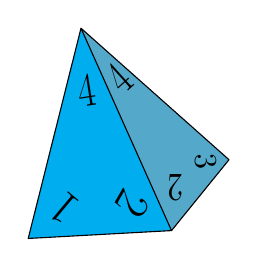
\begin{tikzpicture}[scale=1,line join=round,line cap=round,transform shape]
			\foreach \x\y\t in {0/0/O,1.82/0.1/A,2.55/1./B,0.67/2.67/C}
			\coordinate (\t) at (\x,\y);
			\fill[cyan] (O)--(A)--(C)--cycle;
			\fill[cyan!60!gray] (A)--(B)--(C)--cycle;
			\draw (A)--(B)--(C)--(O)--(A)--(C);
			\node at (O)[shift={(40:0.6)},rotate=140]{\LARGE 1};
			\node at (A)[shift={(145:0.6)},rotate=-120]{\LARGE 2};
			\node at (A)[shift={(85:0.55)},rotate=180,xscale=0.8]{\Large 2};
			\node at (B)[shift={(183:0.3)},rotate=-85,scale=0.8]{\Large 3};
			\node at (C)[shift={(-53:0.8)},rotate=42,xscale=0.75]{\LARGE 4};
			\node at (C)[shift={(-85:0.8)},rotate=9,xscale=0.8]{\LARGE 4};
	\end{tikzpicture}}
	\loigiai{
		Tổng số kết quả có thể xảy ra là $n(\Omega)=4 \cdot 4=16$.\\
		Vì con xúc xắc là cân đối nên $16$ kết quả đều có cùng khả năng xuất hiện.
		\begin{listEX}
			\item Lần gieo thứ nhất có $4$ kết quả có thể xảy ra.\\
			Để thuận lợi cho $A$ thì lần gieo thứ hai chỉ có $1$ kết quả xảy ra (trùng kết quả lần một).\\
			Do đó có $4$ kết quả thuận lợi cho biến cố $A$.\\
			Vậy $\mathrm{P}(A)=\dfrac{4\cdot 1}{16}=\dfrac{1}{4}$.
			\item Do tổng các số xuất hiện trên đỉnh của con xúc xắc trong hai lần gieo luôn lớn hơn $1$ nên $B$ là biến cố chắc chắn, $\mathrm{P}(B)=1$.
			\item Nếu tích hai số là $10$ thì phải có một số chia hết cho $5$ mà không có đỉnh nào của con xúc xắc ghi số chia hết cho $5$ nên $C$ là biến cố không thể, $\mathrm{P}(C)=0$.
			\item Có $2$ trường hợp thuận lợi cho $D$, đó là: 
			\begin{itemize}
				\item Lần một xuất hiện $2$ thì lần hai xuất hiện $1$ hoặc $3$ hoặc $4$.
				\item Lần một xuất hiện $1$ hoặc $3$ hoặc $4$ thì lần hai xuất hiện $2$.
			\end{itemize}
			Có $6$ kết quả thuận lợi cho biến cố $D$ nên $\mathrm{P}(D)=\dfrac{6}{16}=\dfrac{3}{8}$.
		\end{listEX}
	}
\end{vd}

% #2808 | Archive/SP_KhoLatex/ID6_old/10XS2.tex | mã gốc 1D2B5-2
\begin{vd}%[Tex hóa SGK CD-CT HK2,T8/22, Dương Phước Sang]%[1D2B5-2]
	Có $3$ chiếc hộp, hộp A chứa $1$ chiếc bút xanh, $1$ chiếc bút đỏ; hộp B chứa $1$ chiếc bút đỏ, $1$ chiếc bút tím; hộp C chứa $1$ chiếc bút đỏ, $1$ chiếc bút tím. Lấy ra ngẫu nhiên từ mỗi hộp $1$ chiếc bút.
	\begin{listEX}
		\item Hãy vẽ sơ đồ hình cây để mô tả các kết quả có thể xảy ra.
		\item Tính xác suất của biến cố $A$: \lq\lq Trong $3$ bút lấy ra có đúng $1$ bút đỏ\rq\rq.
		\dapso{$\dfrac{3}{8}$}
	\end{listEX}
	\loigiai{
		\begin{listEX}
			\item Kí hiệu $X$ là bút xanh, Đ là bút đỏ, T là bút tím. Các kết quả có thể xảy ra trong $3$ lần lấy bút có thể được mô tả bởi sơ đồ hình cây ở dưới đây.
			
			\begin{tikzpicture}[xscale=1.25,line join=round,line cap=round,>=stealth]
				\foreach \x/\y/\t in {0/3.7/O, -1.6/2.9/a1,1.6/2.9/a2, -2.5/2/b1,-0.8/2/b2,0.8/2/b3,2.5/2/b4, -2.9/1.2/c1,-2.1/1.2/c2,-1.2/1.2/c3,-0.4/1.2/c4,0.4/1.2/c5,1.2/1.2/c6,2.1/1.2/c7,2.9/1.2/c8}
				\coordinate (\t) at (\x,\y);
				\draw (a1)--(O)--(a2);
				\draw (b1)--(a1)--(b2) (b3)--(a2)--(b4);
				\draw (c1)--(b1)--(c2) (c3)--(b2)--(c4) (c5)--(b3)--(c6) (c7)--(b4)--(c8);
				\foreach \t/\g/\l in {a1/115/X,a2/45/Đ,b1/135/Đ,b2/35/T,b3/135/Đ,b4/35/T,c1/180/Đ,c2/0/T,c3/180/Đ,c4/0/T,c5/180/Đ,c6/0/T,c7/180/Đ,c8/0/T}
				\path (\t) node[fill=white,inner sep=1pt,draw,circle]{\l};
				\foreach \t/\n/\P/\K in {c1/X/Đ/Đ,c2/X/Đ/T,c3/X/T/Đ,c4/X/T/T,c5/Đ/Đ/Đ,c6/Đ/Đ/T,c7/Đ/T/Đ,c8/Đ/T/T}{
					\node at ($(\t)-(0,0.7)$){\n};
					\node at ($(\t)-(0,1.2)$){\P};
					\node at ($(\t)-(0,1.7)$){\K};
				}
				\node at (-5,2.9)[right]{Hộp A};
				\node at (-5,2)[right]{Hộp B};
				\node at (-5,1.2)[right]{Hộp C};
				\node at (-5,0.5)[right]{Kết quả};
			\end{tikzpicture}
			\item Có tất cả $8$ kết quả có thể xảy ra, trong đó có $3$ kết quả thuận lợi cho biến cố $A$.\\
			Vậy $\mathrm{P}(A)=\dfrac{3}{8}$.
		\end{listEX}
	}
\end{vd}

% #2809 | Archive/SP_KhoLatex/ID6_old/10XS2.tex | mã gốc 1D2B5-2
\begin{vd}%[Tex hóa SGK CD-CT HK2,T8/22, Dương Phước Sang]%[1D2B5-2]
	Một hộp chứa $10$ tấm thẻ có kích thước như nhau và được đánh số từ $2021$ đến $2030$, mỗi thẻ chỉ ghi đúng một số. Chọn ra ngẫu nhiên đồng thời $3$ thẻ từ hộp.
	\begin{listEX}
		\item Tìm biến cố đối của biến cố $A$: \lq\lq Tích các số ghi trên $3$ thẻ chia hết cho $5$\rq\rq.
		\item Tính xác suất của biến cố $A$.
		\dapso{$\dfrac{8}{15}$}
	\end{listEX}
	\loigiai{
		\begin{listEX}
			\item Biến cố đối của $A$ là $\overline{A}$: \lq\lq Tích các số ghi trên $3$ thẻ không chia hết cho $5$\rq\rq.
			\item Do các thẻ có kích thước như nhau nên chúng có cùng khả năng được chọn.\\
			Số các kết quả có thể xảy ra là $n(\Omega)=\mathrm{C}_{10}^3=120$.\\
			Từ $2021$ đến $2030$ có $8$ số không chia hết cho $5$.\\
			Vì biến cố đối $\overline{A}$ xảy ra khi số trên cả $3$ thẻ đều không chia hết cho $5$ nên số các kết quả thuận lợi cho $\overline{A}$ là $n\left(\overline{A}\right)=\mathrm{C}_8^3=56$.\\
			Xác suất xảy ra biến cố $\overline{A}$ là $P\left(\overline{A}\right)=\dfrac{56}{120}=\dfrac{7}{15}$.\\
			Xác suất xảy ra biến cố $A$ là $\mathrm{P}(A)=1-P\left(\overline{A}\right)=1-\dfrac{7}{15}=\dfrac{8}{15}$.
		\end{listEX} 
	}
\end{vd}

% #2810 | Archive/SP_KhoLatex/ID6_old/10XS2.tex | mã gốc 1D2B5-2
\begin{bt}%[Tex hóa SGK CD-CT HK2,T8/22, Dương Phước Sang]%[1D2B5-2]
	Gieo một con xúc xắc $4$ mặt cân đối và đồng chất ba lần. Tính xác suất của các biến cố:
	\begin{listEX}
		\item \lq\lq Tổng các số xuất hiện ở đỉnh phía trên của con xúc xắc trong ba lần gieo lớn hơn $2$\rq\rq.
		\dapso{$1$}
		\item \lq\lq Có đúng một lần số xuất hiện ở đỉnh phía trên của con xúc xắc là $2$\rq\rq.
		\dapso{$\dfrac{27}{64}$}
	\end{listEX}
	\loigiai{
		\begin{listEX}
			\item Biến cố $A$: \lq\lq Tổng các số xuất hiện ở đỉnh phía trên của con xúc xắc trong $3$ lần gieo lớn hơn $2$\rq\rq là biến cố chắc chắn.\\
			Do đó $A$ có xác suất là $\mathrm{P}(A)=1$.
			\item Số các kết quả có thể xảy ra là $n(\Omega)=4^3=64$.\\
			Gọi $B$ là biến cố \lq\lq Có đúng một lần số xuất hiện ở đỉnh phía trên của con xúc xắc là $2$\rq\rq.\\
			Số các kết quả thuận lợi cho biến cố $B$ là $3 \cdot 3^2=27$.\\
			Vậy $\mathrm{P}(B)=\dfrac{27}{64}$.
		\end{listEX} 
	}
\end{bt}

% #2811 | Archive/SP_KhoLatex/ID6_old/10XS2.tex | mã gốc 1D2B5-2
\begin{bt}%[Tex hóa SGK CD-CT HK2,T8/22, Dương Phước Sang]%[1D2B5-2]
	Tung một đồng xu cân đối và đồng chất bốn lần. Tính xác suất của các biến cố:
	\begin{listEX}
		\item \lq\lq Cả bốn lần đều xuất hiện mặt giống nhau\rq\rq.
		\dapso{$\dfrac{1}{8}$}
		\item \lq\lq Có đúng một lần xuất hiện mặt sấp, ba lần xuất hiện mặt ngửa\rq\rq.
		\dapso{$\dfrac{1}{4}$}
	\end{listEX}
	\loigiai{
		Số các kết quả có thể xảy ra là $n(\Omega)=2^4=16$.
		\begin{listEX}
			\item Gọi $A$ là biến cố \lq\lq Cả bốn lần đều xuất hiện mặt giống nhau\rq\rq.\\
			Số các kết quả thuận lợi cho $A$ là $n(A)=2\cdot 1\cdot 1\cdot 1=2$.\\
			Vậy xác suất của biến cố $A$ là $\mathrm{P}(A)=\dfrac{2}{16}=\dfrac{1}{8}$.
			\item Gọi $B$ là biến cố \lq\lq Có đúng một lần xuất hiện mặt sấp, ba lần xuất hiện mặt ngửa\rq\rq.\\
			Số các kết quả thuận lợi cho $B$ là $n(B)=4$.\\
			Vậy xác suất của biến cố $B$ là $\mathrm{P}(B)=\dfrac{4}{16}=\dfrac{1}{4}$.
		\end{listEX} 
	}
\end{bt}

% #2812 | Archive/SP_KhoLatex/ID6_old/10XS2.tex | mã gốc 1D2B5-2
\begin{bt}%[Tex hóa SGK CD-CT HK2,T8/22, Dương Phước Sang]%[1D2B5-2]
	Chi có $1$ cái ô xanh, $1$ cái ô trắng; $1$ cái mũ xanh, $1$ cái mũ trắng, $1$ cái mũ đen; $1$ đôi giày đen; $1$ đôi giày trắng. Chi chọn ngẫu nhiên $1$ cái ô, $1$ cái mũ và $1$ đôi giày để đến trường.
	\begin{listEX}
		\item Hãy vẽ sơ đồ cây mô tả các kết quả có thể xảy ra.
		\item Tính xác suất của biến cố \lq\lq Chỉ có $1$ trong $3$ thứ đồ Chi chọn có màu trắng\rq\rq.
		\dapso{$\dfrac{5}{12}$}
	\end{listEX}
	\loigiai{
		\begin{listEX}
			\item Ta có sơ đồ hình cây như Hình sau:
			
			\begin{tikzpicture}[xscale=1.8,line join=round,line cap=round,>=stealth]
				\foreach \x/\y/\t in {0/3.7/O,-2/2.9/a1,2/2.9/a2,-3.2/2/b1,-2/2/b2,-0.8/2/b3,0.8/2/b4,2/2/b5,3.2/2/b6,-3.5/1.2/c1,-2.9/1.2/c2,-2.3/1.2/c3,-1.7/1.2/c4,-1.1/1.2/c5,-0.5/1.2/c6,0.5/1.2/c7,1.1/1.2/c8,1.7/1.2/c9,2.3/1.2/c10,2.9/1.2/c11,3.5/1.2/c12}
				\coordinate (\t) at (\x,\y);
				\draw (a1)--(O)--(a2);
				\draw (b1)--(a1)--(b2) (a1)--(b3) (b4)--(a2)--(b5) (a2)--(b6);
				\draw (c1)--(b1)--(c2) (c3)--(b2)--(c4) (c5)--(b3)--(c6) (c7)--(b4)--(c8)  (c9)--(b5)--(c10)  (c11)--(b6)--(c12);
				\foreach \t/\g/\l in {a1/110/X,a2/70/T,
					b1/130/X,b2/35/T,b3/50/Đ,b4/130/X,b5/35/T,b6/50/Đ,
					c1/180/Đ,c2/0/T,c3/180/Đ,c4/0/T,c5/180/Đ,c6/0/T,c7/180/Đ,c8/0/T,c9/180/Đ,c10/0/T,c11/180/Đ,c12/0/T
				}
				\path (\t) node[fill=white,inner sep=1pt,draw,circle]{\l};
				\foreach \t/\n/\P/\k in {c1/X/X/Đ,c2/X/X/T,c3/X/T/Đ,c4/X/T/T,c5/X/Đ/Đ,c6/X/Đ/T,c7/T/X/Đ,c8/T/X/T,c9/T/T/Đ,c10/T/T/T,c11/T/Đ/Đ,c12/T/Đ/T}{
					\node at ($(\t)-(0,0.7)$){\n};
					\node at ($(\t)-(0,1.2)$){\P};
					\node at ($(\t)-(0,1.7)$){\k};
				}
				\node at (-5,2.9)[right]{Ô};
				\node at (-5,2)[right]{Mũ};
				\node at (-5,1.2)[right]{Giày};
				\node at (-5,0.5)[right]{Kết quả};
			\end{tikzpicture}
			\item Xét phép thử \lq\lq Chọn ngẫu nhiên $1$ cái ô, $1$ cái mũ và $1$ đôi giày từ số ô, mũ và giày Chi có\rq\rq.\\
			Phép thử này có số kết quả có thể xảy ra là $n(\Omega)=2\cdot 3\cdot 2=12$.\\ 
			Gọi $A$ là biến cố \lq\lq Chỉ có $1$ trong $3$ thứ đồ Chi chọn có màu trắng\rq\rq thì $n(A)=5$.\\
			Xác suất xảy ra biến cố $A$ là $\mathrm{P}(A)=\dfrac{n(A)}{n(\Omega)}=\dfrac{5}{12}$.
		\end{listEX}
	}
\end{bt}

% #2813 | Archive/SP_KhoLatex/ID6_old/10XS2.tex | mã gốc 1D2B5-2
\begin{bt}%[Tex hóa SGK CD-CT HK2,T8/22, Dương Phước Sang]%[1D2B5-2]
	Chọn ngẫu nhiên $10$ số tự nhiên từ dãy các số tự nhiên từ $1$ đến $100$. Xác định biến cố đối của các biến cố sau:
	\begin{enumerate}
		\item $A$: \lq\lq Có ít nhất $3$ số lẻ trong $10$ số được chọn\rq\rq.
		\item $B$: \lq\lq Tất cả $10$ số được chọn đều là số chẵn\rq\rq.
		\item $C$: \lq\lq Có không quá $5$ số chẵn trong $10$ số được chọn\rq\rq.
	\end{enumerate}
	\loigiai{
		\begin{enumerate}
			\item $A$: \lq\lq Có ít nhất $3$ số lẻ trong $10$ số được chọn\rq\rq.\\
			$\Rightarrow \overline{A}$: \lq\lq Có không quá $2$ số lẻ trong $10$ số được chọn\rq\rq.
			\item $B$: \lq\lq Tất cả $10$ số được chọn đều là số chẵn\rq\rq.\\
			$\Rightarrow \overline{B}$: \lq\lq Có ít nhất $1$ số được chọn là số lẻ\rq\rq.
			\item $C$: \lq\lq Có không quá $5$ số chẵn trong $10$ số được chọn\rq\rq.\\
			$\Rightarrow \overline{C}$: \lq\lq Có ít nhất $6$ số chẵn trong $10$ số được chọn\rq\rq.
		\end{enumerate}
	}
\end{bt}

% #2814 | Archive/SP_KhoLatex/ID6_old/10XS2.tex | mã gốc 1D2T5-2
\begin{bt}%[Tex hóa SGK CD-CT HK2,T8/22, Dương Phước Sang]%[1D2T5-2]
	Trên tường có một đĩa hình tròn có cấu tạo đồng chất và cân đối. 
	\immini{
		Mặt đĩa được chia thành $12$ hình quạt bằng nhau và được đánh số từ $1$ đến $12$. Trọng quay đĩa quanh trục gắn ở tâm $3$ lần và quan sát xem mỗi khi dừng lại mũi tên chỉ vào ô ghi số mấy.\\
		Tính xác suất của các biến cố:
		\begin{enumerate}
			\item $A$: \lq\lq Cả $3$ lần mũi tên đều chỉ vào ô ghi số lẻ\rq\rq.
			\dapso{$\dfrac{1}{8}$}
			\item $B$: \lq\lq Có đúng $2$ lần mũi tên chỉ vào ô ghi số lẻ\rq\rq.
			\dapso{$\dfrac{3}{8}$}
			\item $C$: \lq\lq Tích $3$ số mũi tên chỉ vào là số nguyên tố\rq\rq.
			\dapso{$\dfrac{5}{576}$}
	\end{enumerate}}
	{\vspace{-0.5cm}
		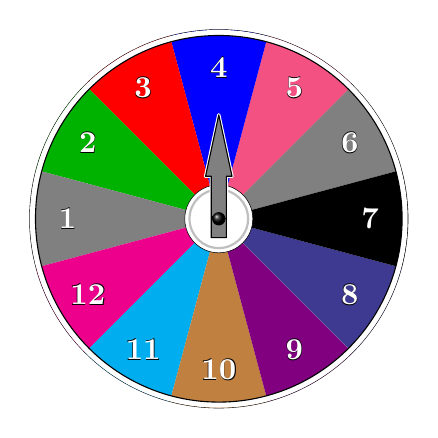
\begin{tikzpicture}[scale=1.2,font=\footnotesize,line join=round,line cap=round,>=stealth]
			\draw[black] (0,0) circle(2);
			\foreach \t/\c in {1/gray,2/yellow!30!magenta,3/blue,4/red,5/green!70!black,6/gray,7/magenta,8/cyan,9/brown,10/violet,11/yellow!10!blue,12/black}
			\fill[\c] (0,0)--(\t*30-15:2)--(\t*30-15:2) arc(\t*30-15:\t*30+15:2)--cycle;
			\draw[white,line width=2.pt] (0,0) circle(1.97);
			\draw[] (0,0) circle(1.94);
			\draw[fill=white, very thin] (0,0) circle(0.36);
			\draw[gray!50,fill=white, thick] (0,0) circle(0.31);
			\draw[white,very thick] (-0.08,-0.2)--(-0.08,0.45)--(-0.14,0.45)--(0,1.1)--(0.14,0.45)--(0.08,0.45)--(0.08,-0.2)--cycle;
			\draw[fill=gray] (-0.08,-0.2)--(-0.08,0.45)--(-0.14,0.45)--(0,1.1)--(0.14,0.45)--(0.08,0.45)--(0.08,-0.2)--cycle;
			\shade[ball color=black] (0,0) circle(2pt);
			\foreach \t in {1,2,...,12}{
				\node at (210-\t*30:1.6){\fontsize{12}{0}\selectfont\color{black}\bf\t};
				\node at (210-\t*30:1.6){\fontsize{11}{0}\selectfont\color{white}\bf\t};
			}
	\end{tikzpicture}}
	\loigiai{
		Số kết quả có thể xảy ra sau $3$ lần quay của Trọng là $n(\Omega)=12^3$.
		\begin{enumerate}
			\item Số kết quả thuận lợi cho $A$ là $n(A)=6^3$.\\
			Xác suất của biến cố $A$ là: $\mathrm{P}(A)=\dfrac{6^3}{12^3}=\dfrac{1}{8}$.
			\item $B$ xảy ra với một trong ba trường hợp sau đây (có $6$ số chẵn và $6$ số lẻ trên đĩa quay):
			\begin{itemize}
				\item[$\bullet$] Trường hợp 1: Lần một mũi tên chỉ số lẻ, hai lần kia mũi tên chỉ số chẵn.
				\item[$\bullet$] Trường hợp 2: Lần hai mũi tên chỉ số lẻ, hai lần kia mũi tên chỉ số chẵn.
				\item[$\bullet$] Trường hợp 3: Lần ba mũi tên chỉ số lẻ, hai lần kia mũi tên chỉ số chẵn.
			\end{itemize}
			Như vậy, số kết quả thuận lợi cho biến cố $B$ là: $n(B)=6^3+6^3+6^3$.\\
			Xác suất của biến cố $A$ là: $\mathrm{P}(B)=\dfrac{6^3\cdot 3}{12^3}=\dfrac{3}{8}$.
			\item Biến cố $C$ xảy ra khi có $2$ lần mũi tên chỉ vào số $1$ và $1$ lần chỉ vào các số nguyên tố $2$, $3$, $5$, $7$, $11$.\\
			Do đó $\mathrm{P}(C)=\dfrac{3 \cdot 5}{12^3}=\dfrac{15}{12^3}=\dfrac{5}{576}$.
		\end{enumerate}
	}
\end{bt}

% #2815 | Archive/SP_KhoLatex/ID6_old/10XS2.tex | mã gốc 1D2K5-2
\begin{bt}%[Tex hóa SGK CD-CT HK2,T8/22, Dương Phước Sang]%[1D2K5-2]
	Một văn phòng A có $15$ nhân viên nam và $20$ nhân viên nữ. Để khảo sát mức độ hài lòng của nhân viên thông qua hình thức phỏng vấn, người ta lần lượt ghi tên của từng nhân viên vào $35$ mẩu giấy giống nhau, từ đó chọn ngẫu nhiên $5$ mẩu giấy.
	\begin{listEX}
		\item Tính xác suất của các biến cố:
		\begin{itemize}
			\item $A$: \lq\lq Trong $5$ người được chọn có $2$ nam, $3$ nữ\rq\rq.
			\dapso{$\dfrac{4275}{11594} \approx 36{,}87\%$}
			\item $B$: \lq\lq Có nhiều nhân viên nữ được chọn hơn nhân viên nam\rq\rq.
			\dapso{$\dfrac{207879}{324632} \approx 64{,}04\%$}
			\item $C$: \lq\lq Có ít nhất một người được chọn là nữ\rq\rq.
			\dapso{$\dfrac{4177}{4216} \approx 99{,}07\%$}
		\end{itemize}
		\item  Biết chị Lan là một nhân viên của văn phòng A. Tính xác suất của biến cố chị Lan được chọn.
		\dapso{$\dfrac{1}{7}$}
	\end{listEX}
	\loigiai{
		Số kết quả chọn $5$ mẩu giấy từ $35$ mẩu giấy là $n(\Omega)=\mathrm{C}_{35}^5$.
		\begin{listEX}
			\item 
			\begin{itemize}
				\item Số kết quả thuận lợi cho biến cố $A$ là $n(A)=\mathrm{C}_{15}^2\mathrm{C}_{20}^3$.\\
				Suy ra $\mathrm{P}(A)=\dfrac{\mathrm{C}_{15}^2\mathrm{C}_{20}^3}{\mathrm{C}_{35}^5} =\dfrac{4275}{11594} \approx 36{,}87\%$.
				\item Số kết quả thuận lợi cho biến cố $B$ là $n(B)=\mathrm{C}_{20}^5+\mathrm{C}_{15}^1\mathrm{C}_{20}^4+\mathrm{C}_{15}^2\mathrm{C}_{20}^3$.\\
				Suy ra $\mathrm{P}(B)=\dfrac{\mathrm{C}_{20}^5+\mathrm{C}_{15}^1\mathrm{C}_{20}^4+\mathrm{C}_{15}^2\mathrm{C}_{20}^3}{\mathrm{C}_{35}^5} =\dfrac{207879}{324632} \approx 64{,}04\%$.
				\item Với $C$: \lq\lq Có ít nhất một người được chọn là nữ\rq\rq\ ta có\\
				$\overline{C}$: \lq\lq Không có nhân viên nữ nào được chọn\rq\rq\ và $n\left(\overline{C}\right)=\mathrm{C}_{15}^5$.\\
				Do đó $\mathrm{P}(C)=1-\mathrm{P}\left(\overline{C}\right)=1-\dfrac{\mathrm{C}_{15}^5}{\mathrm{C}_{35}^5} =\dfrac{4177}{4216} \approx 99{,}07\%$.
			\end{itemize}
			\item Gọi $L$: \lq\lq Chị Lan được chọn\rq\rq. Suy ra $\overline{L}$: \lq\lq Chị Lan không được chọn\rq\rq.\\
			Ta có $n\left(\overline{L}\right)=\mathrm{C}_{34}^5$, do đó xác suất chị Lan được chọn là $1-\dfrac{\mathrm{C}_{34}^5}{\mathrm{C}_{35}^5}=\dfrac{1}{7}$.
		\end{listEX}
	}
\end{bt}

% #2816 | Archive/SP_KhoLatex/ID6_old/10XS2.tex | mã gốc 1D2K5-2
\begin{bt}%[Tex hóa SGK CD-CT HK2,T8/22, Dương Phước Sang]%[1D2K5-2]
	Một hội đồng có đúng $1$ người là nữ. Nếu chọn ngẫu nhiên $2$ người từ hội đồng thì xác suất cả hai người đều là nam là $0{,}8$.
	\begin{listEX}
		\item Chọn ngẫu nhiên $2$ người từ hội đồng, tính xác suất của biến cố có $1$ người nữ trong $2$ người đó.
		\dapso{$0{,}2$}
		\item Hội đồng có bao nhiêu người?
		\dapso{$10$}
	\end{listEX}
	\loigiai{
		\begin{listEX}
			\item Việc chọn $2$ người xảy ra $3$ khả năng:
			\begin{itemize}
				\item[$\bullet$] $A$: \lq\lq Cả $2$ người được chọn đều là nam\rq\rq.
				\item[$\bullet$] $B$: \lq\lq Cả $2$ người được chọn đều là nữ\rq\rq.
				\item[$\bullet$] $C$: \lq\lq Có đúng $1$ người nữ được chọn\rq\rq.
			\end{itemize}
			Do hội đồng chỉ có $1$ người nữ nên $B=\varnothing$. Từ đó $C=\overline{A}$.\\
			Vậy $\mathrm{P}(C)=1-\mathrm{P}(A)=0{,}2$.
			\item Gọi $n$ là số người nam trong hội đồng $\left(n \in \mathbb{N}^*,\ n \geq 2\right)$.\\
			Xác suất để $2$ người được chọn ra đều là nam là $\dfrac{\mathrm{C}_n^2}{\mathrm{C}_{n+1}^2}=\dfrac{n-1}{n+1}=0{,}8$. Suy ra $n=9$.\\
			Vậy hội đồng có $10$ người.
		\end{listEX}
	}
\end{bt}

% #2817 | Archive/SP_KhoLatex/ID6_old/10XS2.tex | mã gốc 1D2K5-2
\begin{bt}%[Tex hóa SGK CD-CT HK2,T8/22, Dương Phước Sang]%[1D2K5-2]
	An, Bình, Cường và $2$ bạn nữa xếp ngẫu nhiên thành một hàng ngang để chụp ảnh. Tính xác suất của các biến cố:
	\begin{listEX}[2]
		\item \lq\lq An và Bình đứng ở hai đầu hàng\rq\rq.
		\dapso{$\dfrac{1}{10}$}
		\item \lq\lq Bình và Cường đứng cạnh nhau\rq\rq.
		\dapso{$\dfrac{2}{5}$}
		\item \lq\lq An, Bình, Cường đứng cạnh nhau\rq\rq.
		\dapso{$\dfrac{3}{10}$}
	\end{listEX}
	\loigiai{
		Xếp An, Bình, Cường và $2$ bạn nữa thành một hàng ngang thì có số kết quả là $n(\Omega)=5!$
		\begin{listEX}
			\item Biến cố $A$: \lq\lq An và Bình đứng ở hai đầu hàng\rq\rq có $n(A)=2\cdot 3!$.\\
			Vậy $\mathrm{P}(A)=\dfrac{2 \cdot 3!}{5!}=\dfrac{1}{10}$.
			\item Gọi $B$: \lq\lq Bình và Cường đứng cạnh nhau\rq\rq.\\
			Để $B$ xảy ra, trước tiên ta xếp chỗ cho $\mathcal{N}$ (đại diện Bình, Cường) và $3$ bạn còn lại (khác Bình Cường). Sau đó xếp $2$ bạn Bình, Cường vào đúng vị trí chỗ của $\mathcal{N}$.\\
			Vậy $n(B)=4!\cdot 2!$, do đó $\mathrm{P}(B)=\dfrac{4! \cdot 2!}{5!}=\dfrac{2}{5}$.
			\item Gọi $C$: \lq\lq An, Bình, Cường đứng cạnh nhau\rq\rq.\\
			Để $C$ xảy ra, trước tiên ta xếp chỗ cho $\mathcal{M}$ (đại diện An, Bình, Cường) và $2$ bạn còn lại (khác An, Bình Cường). Sau đó xếp $3$ bạn An, Bình, Cường vào đúng vị trí chỗ của $\mathcal{M}$.\\
			Vậy $n(C)=3!\cdot 3!$, do đó $\mathrm{P}(C)=\dfrac{3!\cdot 3!}{5!}=\dfrac{3}{10}$.
		\end{listEX}
	}
\end{bt}

% #2818 | Archive/SP_KhoLatex/ID6_old/10XS2.tex | mã gốc 1D2K5-2
\begin{bt}%[Tex hóa SGK CD-CT HK2,T8/22, Dương Phước Sang]%[1D2K5-2]
	Một hộp kín có $1$ quả bóng xanh và $5$ quả bóng đỏ có kích thước và khối lượng bằng nhau. Hỏi Dũng cần lấy ra từ hộp ít nhất bao nhiêu quả bóng để xác suất lấy được quả bóng xanh lớn hơn $0{,}5$?
	\dapso{$4$}
	\loigiai{
		Xét phép thử \lq\lq Dũng lấy ra $k$ quả bóng từ hộp\rq\rq\ $\left(k \in \mathbb{N}^{*},\ k \leq 6\right)$.\\
		Số kết quả có thể xảy ra của phép thử này là $n(\Omega)=\mathrm{C}_6^k$.\\
		Xét biến cố $A$: \lq\lq Có $1$ quả bóng xanh được Dũng lấy ra\rq\rq.\\
		Biến cố $A$ có $n(A)=\mathrm{C}_6^k-\mathrm{C}_5^k$.\\
		Do đó xác suất để trong $k$ quả bóng được Dũng lấy ra có quả màu xanh là
		$$\begin{aligned}
			\mathrm{P}(A)=\dfrac{\mathrm{C}_6^k-\mathrm{C}_5^k}{\mathrm{C}_6^k}
			&=\dfrac{\dfrac{6!}{(6-k)!\cdot k!}-\dfrac{5!}{(5-k)!\cdot k!}}{\dfrac{6!}{(6-k)!\cdot k!}}\\
			&=1-\dfrac{5!}{(5-k)!\cdot k!} \cdot \dfrac{(6-k)!\cdot k!}{6!}\\
			&=1-\dfrac{5!}{(5-k)!\cdot k!} \cdot \dfrac{(6-k)(5-k)!\cdot k!}{6\cdot 5!}\\
			&=1-\dfrac{6-k}{6}\\
			&=\dfrac{k}{6}
		\end{aligned}$$
		Như vậy $\mathrm{P}(A)>0{,}5 \Leftrightarrow \dfrac{k}{6}>0{,}5 \Leftrightarrow k>3$, tức là Dũng phải lấy ít nhất $4$ quả bóng.
	}
\end{bt}

% #2819 | Archive/SP_KhoLatex/ID6_old/10XS2.tex | mã gốc 1D2K5-2
\begin{bt}%[Tex hóa SGK CD-CT HK2,T8/22, Dương Phước Sang]%[1D2K5-2]
	Bốn đội bóng A, B, C, D lọt vào vòng bán kết của một giải đấu. Ban tổ chức bốc thăm chia $4$ đội này thành $2$ cặp đấu một cách ngẫu nhiên. Tính xác suất của biến cố hai đội A và B đấu với nhau ở trận bán kết.
	\dapso{$\dfrac{1}{3}$}
	\loigiai{
		Số kết quả chia $4$ đội thành $2$ cặp đấu (có tính thứ tự giữa $2$ cặp) là $n(\Omega)=\mathrm{C}_4^2=6$.\\
		Có $2$ cách để đội A và đội B gặp nhau ở bán kết (là cặp đấu $1$ hoặc cặp đấu $2$).\\
		Vậy xác suất cần tìm là $p=\dfrac{2}{6}=\dfrac{1}{3}$.
	}
\end{bt}

% #2830 | Archive/SP_KhoLatex/ID6_old/0D5-B2.tex | mã gốc 1D2B2-1
\begin{vd}%[Thi thử L1, THPT Trần Phú - Đà Nẵng, 2018]%[1D2B2-1]%[Lê Thanh Nin, dự án(12EX-8)]
	Một tổ có $10$ học sinh. Hỏi có bao nhiêu cách chọn ra $2$ học sinh từ tổ đó để giữ hai chức vụ tổ trưởng và tổ phó?
	\hspace*{6cm} {\sf\fontsize{10pt}{1pt}\selectfont Đáp số: 90.}
	\loigiai{
		Mỗi cách chọn $2$ học sinh giữ hai chức vụ tổ trưởng và tổ phó là một chỉnh hợp chập $2$ của $10$. Vậy số cách chọn là  $\mathrm{A}_{10}^2$}
\end{vd}

% #2831 | Archive/SP_KhoLatex/ID6_old/0D5-B2.tex | mã gốc 1D2Y2-1
\begin{vd}%[Đề thi thử lần 1, An Phước, Ninh Thuận 2018%[QK Trương, Dự án (12EX-10)]%[1D2Y2-1]
	Cho đa giác đều có $10$ đỉnh. Tìm số véc-tơ khác véc-tơ-không có điểm đầu và điểm cuối là các đỉnh của đa giác. 
	\hspace*{5cm} {\sf\fontsize{10pt}{1pt}\selectfont Đáp số: 90.}
	\loigiai{
		Số véc-tơ khác véc-tơ-không có điểm đầu và điểm cuối là các đỉnh của đa giác có $ 10 $ đỉnh là $ \mathrm{A}_{10}^2 =90$. }
\end{vd}

% #2832 | Archive/SP_KhoLatex/ID6_old/0D5-B2.tex | mã gốc 1D2B2-1
\begin{vd}%[Đề TT THCS và THPT M.V Lômônôxốp - Hà Nội, 2018]%[Đỗ Đường Hiếu (dự án 12EX-11)]%[1D2B2-1]
	Cho tập $X=\{1; 2; 3; 4; 5; 6\}$. Có bao nhiêu số tự nhiên có ba chữ số đôi một khác nhau được tạo thành từ tập $X$? 
	\hspace*{5cm} {\sf\fontsize{10pt}{1pt}\selectfont Đáp số: 120.}
	\loigiai{
		Mỗi số tự nhiên có ba chữ số khác nhau được tạo thành từ tập $X$ là một chỉnh hợp chập $3$ của tập $X$. Cho nên, số các số tự nhiên có ba chữ số đôi một khác nhau được tạo thành từ tập $X$ là $\mathrm{A}^3_6=120$ số.
	}
\end{vd}

% #2833 | Archive/SP_KhoLatex/ID6_old/0D5-B2.tex | mã gốc 1D2B2-1
\begin{vd}%[Đề KSCL THPT Quốc gia 2018 môn Toán trường THPT Phước Vĩnh $-$ Bình Dương]%[Trần Minh, Dự án (12EX-11)]%[1D2B2-1]
	Từ các số $1$, $2$, $3$, $4$, $5$, $7$. Từ các số trên có thể lập được bao nhiêu số tự nhiên có $4$ chữ số khác nhau và chia hết cho $5$?
	\hspace*{5cm} {\sf\fontsize{10pt}{1pt}\selectfont Đáp số: 60.}
	\loigiai{
		Theo bài ra chữ số hàng đơn vị có $1$ cách chọn.\\
		Ba chữ số còn lại có $\mathrm{A}_5^3=60$ cách.\\
		Vậy có $60$ số.}
\end{vd}

% #2835 | Archive/SP_KhoLatex/ID6_old/0-GK1-4-ChuyenHaLong-2223.tex | mã gốc 1D2G3-3
\begin{bt}%[Đề kiểm tra GHK1 môn Toán 10 trường THPT Chuyên Hạ Long]%[Lê Văn Tuyến, 10EX-HK1-2223]%[1D2G3-3]
	Tính tổng $$S=\mathrm{C}_{2022}^0+2\mathrm{C}_{2022}^1+3\mathrm{C}_{2022}^2+\ldots+2023\mathrm{C}_{2022}^{2022}.$$
	\loigiai{
		Ta có 
		\begin{eqnarray*}
			S&=&\mathrm{C}_{2022}^0+2\mathrm{C}_{2022}^1+3\mathrm{C}_{2022}^2+\cdots+2023\mathrm{C}_{2022}^{2022} \quad (1)\\
			&=&2023\mathrm{C}_{2022}^{2022} + 2022C_{2022}^{2021}+\cdots+2\mathrm{C}_{2022}^1+\mathrm{C}_{2022}^0. \end{eqnarray*}
		Vì $\mathrm{C}_n^k=\mathrm{C}_n^{n-k}$ nên $S=2023\mathrm{C}_{2022}^{0} + 2022\mathrm{C}_{2022}^{1}+\cdots+2\mathrm{C}_{2022}^{2021}+\mathrm{C}_{2022}^{2022}$.\quad (2)\\
		Cộng $(1)$ và $(2)$ ta có 
		\begin{eqnarray*}
				2S&=&2024\left(\mathrm{C}_{2022}^0+\mathrm{C}_{2022}^1+\mathrm{C}_{2022}^2+\cdots+\mathrm{C}_{2022}^{2022}\right)\\
			\Leftrightarrow S&=&1012\left(\mathrm{C}_{2022}^0+\mathrm{C}_{2022}^1+\mathrm{C}_{2022}^2+\cdots+\mathrm{C}_{2022}^{2022}\right)\\
			&=& 1012\cdot 2^{2022}. \end{eqnarray*}
	}
\end{bt}

% #2859 | Archive/SP_KhoLatex/ID6_old/1D2G2-1.tex | mã gốc 1D2G2-1
\begin{ex}%[Tác giả: Trần Minh Đức, FB: Trần Minh Đức, Email: Minhduc486@gmail.com]%[WTT-VDC-6-1D2, Lê Hồng Phi]%[1D2G2-1]
Có bao nhiêu cách điền các số $1, 2, 3, 4, 5, 6$ (mỗi số một lần) vào các ô tròn ở trên Hình $1$ sao cho tổng các số ở mỗi cạnh của tam giác là bằng nhau? (ví dụ ở Hình $2$, tổng các số ở mỗi cạnh đều bằng 10).
\begin{longtable}{m{0.3\textwidth}m{0.3\textwidth}}
	\begin{tikzpicture}[scale=1,
	>=stealth,auto,every node/.style={draw,circle}]
	\node[minimum size=1cm] (a) at (0,0)  {};
	\node[minimum size=1cm] (b) at (4,0)  {};
	\node[minimum size=1cm] (c) at (60:4) {};
	\node[minimum size=1cm] (m) at ($(a)!.5!(b)$) {};
	\node[minimum size=1cm] (n) at ($(c)!.5!(b)$) {};
	\node[minimum size=1cm] (p) at ($(a)!.5!(c)$) {};
	\draw (a) edge (m);
	\draw (m) edge (b);
	\draw (b) edge (n);
	\draw (n) edge (c);
	\draw (c) edge (p);
	\draw (p) edge (a);
	\end{tikzpicture} &	
	\begin{tikzpicture}[scale=1,
	>=stealth,auto,every node/.style={draw,circle}]
	\node[minimum size=1cm] (a) at (0,0)  {$3$};
	\node[minimum size=1cm] (b) at (4,0)  {$5$};
	\node[minimum size=1cm] (c) at (60:4) {$1$};
	\node[minimum size=1cm] (m) at ($(a)!.5!(b)$) {$2$};
	\node[minimum size=1cm] (n) at ($(c)!.5!(b)$) {$4$};
	\node[minimum size=1cm] (p) at ($(a)!.5!(c)$) {$6$};
	\draw (a) edge (m);
	\draw (m) edge (b);
	\draw (b) edge (n);
	\draw (n) edge (c);
	\draw (c) edge (p);
	\draw (p) edge (a);
	\end{tikzpicture}\\
	\centerline{Hình 1} & \centerline{Hình 2}
\end{longtable}
\loigiai{
\immini{Gọi các số điền vào là $ A_1, A_2, A_3,  B_1, B_2, B_3$ như hình vẽ.\\
	Ta có \begin{eqnarray*}
	&&A_1+ B_2+ A_3= A_1+ B_3+ A_2= A_2+  B_1+ A_3\\
	&\Leftrightarrow &\heva{& A_1+ B_2+ A_3= A_1+ B_3+ A_2 \\ &A_1+ B_2+ A_3= A_2+  B_1+ A_3}\\
	&\Leftrightarrow & \heva{&  A_3- B_3= A_2- B_2 \\ &  A_1-  B_1= A_2- B_2}\\
	&\Leftrightarrow &  A_1-  B_1= A_2- B_2= A_3- B_3.
	\end{eqnarray*}}{\begin{tikzpicture}[scale=1,
	>=stealth,auto,every node/.style={draw,circle}]
	\node[minimum size=1cm] (a) at (0,0)  {$A_2$};
	\node[minimum size=1cm] (b) at (4,0)  {$A_3$};
	\node[minimum size=1cm] (c) at (60:4) {$A_1$};
	\node[minimum size=1cm] (m) at ($(a)!.5!(b)$) {$B_1$};
	\node[minimum size=1cm] (n) at ($(c)!.5!(b)$) {$B_2$};
	\node[minimum size=1cm] (p) at ($(a)!.5!(c)$) {$B_3$};
	\draw (a) edge (m);
	\draw (m) edge (b);
	\draw (b) edge (n);
	\draw (n) edge (c);
	\draw (c) edge (p);
	\draw (p) edge (a);
	\end{tikzpicture}}\noindent
Do $ A_1, A_2, A_3,  B_1, B_2, B_3$ là một hoán vị của $1, 2, 3, 4, 5, 6$.
Nên ta chỉ có các bộ sau thỏa mãn: $6-5 = 4-3 = 2-1;\ 5-6 = 3-4 = 1-2;\ 6-3 = 5-2 = 4-1;\  3-6 = 2-5 = 1-4$.\\
Ứng với mỗi bộ ở trên ta có $3!$ hoán vị các đỉnh $ A_1, A_2, A_3$.
Và với mỗi cách chọn $ A_1, A_2, A_3$ thì sẽ có duy nhất một cách chọn $B_1, B_2, B_3$.\\
Vậy có $3!\times 4=24$ cách điền thỏa mãn yêu cầu bài toán.
}
\end{ex}

% #2861 | Archive/SP_KhoLatex/ID6_old/1D2Y1-3.tex | mã gốc 1D2Y1-3
\begin{bt}%[Dự án 11EX-XS-TH, Sang Nguyen, 2019]%[1D2Y1-3] 
	Cho $5$ chữ số: $0$, $1$, $2$, $3$, $4$. Từ $5$ chữ số đó, có thể lập được bao nhiêu chữ số chẵn có $5$ chữ số sao cho trong mỗi số đó, mỗi chữ số trên có mặt một lần?
	\dapso{$60$}
	\loigiai
	{
		Gọi $\overline{n}=\overline{abcde}$ là số cần tìm.
		\begin{enumerate}[TH 1.]
			\item Chọn $e=0$ có $1$ cách chọn.\\
			$a$ có $4$ cách chọn.\\
			$b$ có $3$ cách chọn.\\
			$c$ có $2$ cách chọn.\\
			$d$ có $1$ cách chọn.\\
			Trong trường hợp này có $1\cdot4\cdot3\cdot2\cdot1=24$ số $\overline{n}$ cần tìm.
			\item Chọn $e=2$ hoặc $e=4$ có $2$ cách chọn.\\
			$a \ne 0$ và $a \ne e$ có $3$ cách chọn.\\
			$b$ có $3$ cách chọn.\\
			$c$ có $2$ cách chọn.\\
			$d$ có $1$ cách chọn.\\
			Trong trường hợp này có $2\cdot3\cdot3\cdot2\cdot1=36$ số $\overline{n}$ cần tìm.
		\end{enumerate}
		Vậy có tất cả $24+36=60$ số $\overline{n}$ cần tìm.
	}
\end{bt}

% #2868 | Archive/SP_KhoLatex/ID6_old/0D5-B3.tex | mã gốc 1D2B2-1
\begin{vd}%[1D2B2-1]
	Một tổ công nhân có $12$ người. Cần chọn $3$ người để đi làm cùng một nhiệm vụ, hỏi có bao nhiêu cách chọn?
	\hspace*{6cm} {\sf\fontsize{10pt}{1pt}\selectfont Đáp số: 220 }
	\loigiai
	{Chọn $3$ người từ $12$ người đi thực hiện cùng một nhiệm vụ là một tổ hợp chập $3$ của $12$ phần tử.\\
		Số cách chọn là $\mathrm{C}_{12}^3$.
	}
\end{vd}

% #2869 | Archive/SP_KhoLatex/ID6_old/0D5-B3.tex | mã gốc 1D2B2-1
\begin{vd}%[1D2B2-1]
	Giải bóng đá AFF-CUP $2018$ có tất cả $10$ đội bóng tham gia, chia đều làm hai bảng $A$ và $B$. Ở vòng đấu bảng, mỗi đội bóng thi đấu với mỗi đội bóng cùng bảng $1$ trận. Hỏi tại vòng bảng các đội thi đấu tổng cộng bao nhiêu trận?	
	\hspace*{3cm} {\sf\fontsize{10pt}{1pt}\selectfont Đáp số: 20}
	\loigiai{
		Mỗi bảng có $5$ đội bóng.\\
		Mỗi đội bóng thi đấu với mỗi đội bóng cùng bảng $1$ trận nên số trận thi đấu trong mỗi bảng bằng số cách chọn $2$ đội bóng từ $5$ đội, tức là $\mathrm{C}_5^2=10$ trận.\\
		Vì có hai bảng nên tổng số trận đấu ở vòng bảng là $20$ trận.
	}
\end{vd}

% #2870 | Archive/SP_KhoLatex/ID6_old/0D5-B3.tex | mã gốc 1D2K2-1
\begin{vd}%[1D2K2-1]
	Có $20$ bông hoa trong đó có $8$ bông đỏ, $7$ bông vàng, $5$ bông trắng. Chọn ngẫu nhiên $4$ bông để
	tạo thành một bó. Có bao nhiên cách chọn để bó hoa có cả $3$ màu?
	\loigiai{
		Số cách chọn được một bó hoa có $2$ hoa đỏ, $1$ hoa vàng và $1$ hoa trắng là $\mathrm{C}_8^2\mathrm{C}_7^1\mathrm{C}_5^1=980$. Số cách chọn được một bó hoa có $1$ hoa đỏ, $2$ hoa vàng và $1$ hoa trắng là $\mathrm{C}_8^1\mathrm{C}_7^2\mathrm{C}_5^1=840$. Số cách chọn được một bó hoa có $1$ hoa đỏ, $1$ hoa vàng và $2$ hoa trắng là $\mathrm{C}_8^1\mathrm{C}_7^1\mathrm{C}_5^2=560$. Do đó số cách chọn được bó hoa có cả $3$ màu là
		$$980+840+560=2380.$$	
	}
\end{vd}

% #2871 | Archive/SP_KhoLatex/ID6_old/0D5-B3.tex | mã gốc 1D2G2-1
\begin{vd}%[TT Sở Ninh Bình 2018]%[TranTony, 12EX-11]%[1D2G2-1]
	Cho hai đường thẳng $d_1$ và $d_2$ song song với nhau. Trên $d_1$ có $10$ điểm phân biệt, trên $d_2$ có $n$ điểm phân biệt ($n\geq 2$). Biết rằng có $1725$ tam giác có các đỉnh là ba trong số các điểm thuộc $d_1$ và $d_2$ nói trên. Tìm $n$.
	\loigiai{
		Số cách chọn ba điểm trong $n+10$ điểm đã cho là $\mathrm{C}_{n+10}^3$.\\
		Số cách chọn ba điểm trong $10$ trên $d_1$ là $\mathrm{C}_{10}^3$.\\
		Số cách chọn ba điểm trong $n$ trên $d_2$ là $\mathrm{C}_n^3$.\\
		Số tam giác được tạo thành là $\mathrm{C}_{n+10}^3-\mathrm{C}_{10}^3-\mathrm{C}_n^3$.\\
		Từ giả thiết ta có phương trình $\mathrm{C}_{n+10}^3-\mathrm{C}_{10}^3-\mathrm{C}_n^3=1725.$\hfill $(1)$\\
		$(1)\Leftrightarrow\dfrac{(n+10)(n+9)(n+8)}{6}-120-\dfrac{n(n-1)(n-2)}{6}=1725\Leftrightarrow\hoac{&n=15\\&n=-23.}$\\
		Vì $n\geq 2$ nên $n=15$.
	}
\end{vd}

% #2882 | Archive/SP_KhoLatex/ID6_old/1-CK1-OT-De-25.tex | mã gốc 1D2G3-4
\begin{bt}%[1D2G3-4]
	Tìm tất cả các giá trị của tham số $m$ để phương trình sau có ba nghiệm phân biệt lập thành một cấp số nhân $x^3-\left(3m+1\right){x^2}+\left(5m+4\right)x-8=0$.
	\loigiai{
		Giả sử phương trình đã cho có ba nghiệm lập thành cấp số nhân là $x_1$, $x_2$, $x_3$ thì
		$$x^3-\left(3m+1\right){x^2}+\left(5m+4\right)x-8=\left(x-x_1\right)\left(x-x_2\right)\left(x-x_3\right)$$
		Đồng nhất hệ số tự do hai vế, ta được $x_1x_2x_3=8$.\\
		Do $x_1$, $x_2$, $x_3$ tạo thành cấp số nhân nên $x_1x_3=x_2^2$.\\
		Từ hai điều trên suy ra $x_2^3=8\Leftrightarrow{x_2}=2$.\\
		Thay $x=2$ vào phương trình đã cho, ta được $4-2m=0$ $\Leftrightarrow m=2$.\\
		Thử lại, với $m=2,$ ta có phương trình\\
		$$x^3-7x^2+14x-8=0 \Leftrightarrow \hoac{&x=1\\
			&x=2\\
			&x=4.
		}$$
		Ba nghiệm này lập thành một cấp số nhân nên $m=2$ là giá trị cần tìm.}
\end{bt}

% #2883 | Archive/SP_KhoLatex/ID6_old/10XS1.tex | mã gốc 1D2B4-1
\begin{vd}%[Tex hóa SGK CT,T7/22, Hiếu Phan]%[1D2B4-1]
	Minh muốn gọi điện cho Ngọc nhưng Minh quên mất chữ số cuối cùng của số điện thoại. Minh chọn ngẫu nhiên một chữ số cho chữ số cuối cùng để gọi thử.
	\begin{enumEX}[a)]{1}
		\item Mô tả không gian mẫu của phép thử.
		\item Gọi $A$ là biến cố chữ số Minh chọn là số chia hết cho $3$. Viết tập hợp mô tả biến cố $A$.
		\item Gọi $B$ là biến cố chữ số Minh chọn là hợp số. Hỏi có bao nhiêu kết quả thuận lợi cho biến cố $B$?
	\end{enumEX}
	\loigiai{
		\begin{enumEX}[a)]{1}
			\item Không gian mẫu của phép thử $\Omega =\big\{0;1;2;3;4;5;6;7;8;9\big\}$.
			\item Tập hợp mô tả biến cố $A$ là $A=\big\{0;3;6;9\big\}$.
			\item $B=\big\{4;6;8;9\big\}$. Có 4 kết quả thuận lợi cho biến cố $B$.
		\end{enumEX}
	}
\end{vd}

% #2884 | Archive/SP_KhoLatex/ID6_old/10XS1.tex | mã gốc 1D2B4-1
\begin{vd}%[Tex hóa SGK CT,T7/22, Hiếu Phan]%[1D2B4-1]
	Một hộp kín chứa $4$ tấm thẻ có kích thước giống nhau. Mỗi thẻ được ghi một trong các chữ cái $A, B, C, D$; hai thẻ khác nhau được ghi hai chữ khác nhau. Mô tả không gian mẫu của các phép thử sau
	\begin{enumEX}[a)]{1}
		\item Lấy ra ngẫu nhiên lần lượt, không hoàn lại hai thẻ từ hộp.
		\item Lấy ra ngẫu nhiên đồng thời hai thẻ từ hộp.
	\end{enumEX}
	\loigiai{
		\begin{enumEX}[a)]{1}
			\item Không gian mẫu $\Omega =\big\{AB;AC;AD;BA;BC;BD;CA;CB;CD;DA;DB;DC\big\}$.\\
			Trong đó ta kí hiệu $AB$ là kết quả lần thứ nhất lấy được thẻ ghi chữ $A$, lần thứ hai lấy được thẻ ghi chữ $B$.
			\item Không gian mẫu $\Omega =\left\{\{A;B\};\big\{A;C\big\};\big\{A;D\big\};\big\{B;C\big\};\big\{B;D\big\};\big\{C;D\big\}\right\}$.\\
			Trong đó ta kí hiệu $\big\{A;B\big\}$ là kết quả lấy được $1$ thẻ ghi chữ $A$ và $1$ thẻ ghi chữ $B$.
		\end{enumEX}
	}
\end{vd}

% #2885 | Archive/SP_KhoLatex/ID6_old/10XS1.tex | mã gốc 1D2K4-1
\begin{vd}%[Tex hóa SGK CT,T7/22, Hiếu Phan]%[1D2K4-1]
	Hộp thứ nhất chứa $4$ quả bóng được đánh số từ $1$ đến $4$. Hộp thứ hai chứa $5$ quả bóng được đánh số từ $1$ đến $5$. Chọn ngẫu nhiên từ mỗi hộp $1$ quả bóng.
	\begin{enumEX}[a)]{1}
		\item Mô tả không gian mẫu của phép thử.
		\item Viết tập hợp mô tả cho biến cố \lq\lq Tổng các số ghi trên hai quả bóng lớn hơn $7$\rq\rq.
		\item Có bao nhiêu kết quả thuận lợi cho biến cố \lq\lq Tổng các số ghi trên hai quả bóng không vượt quá $7$\rq\rq?
	\end{enumEX}
	\loigiai{
		\begin{enumEX}[a)]{1}
			\item Không gian mẫu $\Omega =\left\{(i;j)\mid 1 \leq i \leq 4{,}1 \leq j \leq 5\right\}$.\\
			Trong đó $(i;j)$ kí hiệu kết quả lấy được bóng ghi số $i$ ở hộp thứ nhất và quả bóng ghi số $j$ ở hộp thứ hai.
			\item Tập hợp mô tả cho biến cố \lq\lq Tổng các số ghi trên hai quả bóng lớn hơn 7\rq\rq\,là $\big\{(3;5);(4;4);(4;5)\big\}$.
			\item Tổng số các kết quả có thể xảy ra khi chọn bóng là $4 \cdot 5=20$.\\
			Có $3$ kết quả thuận lợi cho biến cố \lq\lq Tổng các số ghi trên hai quả bóng lớn hơn 7\rq\rq\,nên số các kết quả thuận lợi cho biến cố \lq\lq Tổng các số ghi trên hai quả bóng không vượt quá 7\rq\rq\, là $20-3=17$.
		\end{enumEX}
	}
\end{vd}

% #2886 | Archive/SP_KhoLatex/ID6_old/10XS1.tex | mã gốc 1D2B4-1
\begin{bt}%[Tex hóa SGK CT,T7/22, Hiếu Phan]%[1D2B4-1]
	Gieo một con xúc xắc bốn mặt cân đối hai lần liên tiếp và quan sát số ghi trên đỉnh của con xúc xắc.
	\begin{enumEX}[a)]{1}
		\item Hãy mô tả không gian mẫu của phép thử.
		\item Hãy viết tập hợp các kết quả thuận lợi cho biến cố \lq\lq Số xuất hiện ở lần gieo thứ hai gấp $2$ lần số xuất hiện ở lần gieo thứ nhất\rq\rq.
	\end{enumEX}
	\loigiai{
		\begin{enumEX}[a)]{1}
			\item Không gian mẫu của phép thử là
			$$ \Omega =\big\{(1;1);(1;2);(1;3);(1;4);(2;1);(2;2);(2;3);(2;4);\\(3;1);(3;2);(3;3);
			(3;4);(4;1);(4;2);(4;3);(4;4)\big\}.$$
			\item Tập hợp mô tả cho biến cố \lq\lq Số xuất hiện ở lần gieo thứ hai gấp $2$ lần số xuất hiện ở lần gieo thứ nhất\rq\rq\,là $\big\{(1;2);(2;4)\big\}$.
		\end{enumEX}
	}
\end{bt}

% #2887 | Archive/SP_KhoLatex/ID6_old/10XS1.tex | mã gốc 1D2Y4-1
\begin{bt}%[Tex hóa SGK CT,T7/22, Hiếu Phan]%[1D2Y4-1]
	Tung một đồng xu ba lần liên tiếp. Phát biểu mỗi biến cố sau dưới dạng mệnh đề $A=\big\{SSS;NSS;SNS;NNS\big\}; B=\big\{SSN;SNS;NSS\big\}$.
	\loigiai{
		\begin{itemize}
			\item $A$: \lq\lq Lần tung thứ ba xuất hiện mặt sấp\rq\rq.
			\item $B$: \lq\lq Có đúng một lần tung xuất hiện mặt ngửa\rq\rq.
		\end{itemize}
	}
\end{bt}

% #2888 | Archive/SP_KhoLatex/ID6_old/10XS1.tex | mã gốc 1D2B4-1
\begin{bt}%[Tex hóa SGK CT,T7/22, Hiếu Phan]%[1D2B4-1]
	Một hộp chứa $5$ quả bóng xanh, $4$ quả bóng đỏ có kích thước và khối lượng như nhau. Hãy mô tả không gian mẫu của phép thử lấy ra ngẫu nhiên một quả bóng từ hộp.
	\loigiai{
		Kí hiệu $5$ quả bóng xanh lần lượt là $X_1,X_2,X_3,X_4,X_5$ và $4$ quả bóng đỏ lần lượt là $D_1, D_2, D_3, D_4$.\\
		Không gian mẫu của phép thử là 
		$\Omega =\big\{X_1;X_2;X_3;X_4;X_5;D_1;D_2;D_3;D_4\big\}$.
	}
\end{bt}

% #2889 | Archive/SP_KhoLatex/ID6_old/10XS1.tex | mã gốc 1D2K4-1
\begin{bt}%[Tex hóa SGK CT,T7/22, Hiếu Phan]%[1D2K4-1]
	Trường mới của bạn Dũng có $3$ câu lạc bộ ngoại ngữ là câu lạc bộ tiếng Anh, câu lạc bộ tiếng Bồ Đào Nha và câu lạc bộ tiếng Campuchia.
	\begin{enumEX}[a)]{1}
		\item Dũng chọn ngẫu nhiên $1$ câu lạc bộ ngoại ngữ để tìm hiểu thông tin. Hãy mô tả không gian mẫu của phép thử nêu trên.
		\item Dũng thử chọn ngẫu nhiên $1$ câu lạc bộ ngoại ngữ để tham gia trong học kì $1$ và $1$ câu lạc bộ ngoại ngữ khác để tham gia trong học kì $2$. Hãy mô tả không gian mẫu của phép thử nêu trên.
	\end{enumEX}
	\loigiai{
		\begin{enumEX}[a)]{1}
			\item $\Omega =\big\{A;B;C\big\}$ trong đó $A,B,C$ lần lượt kí hiệu kết quả Dũng chọn câu lạc bộ tiếng Anh, câu lạc bộ tiếng Bồ Đào Nha và câu lạc bộ tiếng Campuchia.
			\item $\Omega =\big\{AB;AC;BC;BA;CA;CB\big\}$ trong đó $AB$ kí hiệu kết quả Dũng tham gia câu lạc bộ tiếng Anh trong học kì 1, câu lạc bộ tiếng Bồ Đào Nha trong học kì 2,$\ldots$.
		\end{enumEX}
	}
\end{bt}

% #2890 | Archive/SP_KhoLatex/ID6_old/10XS1.tex | mã gốc 1D2B4-1
\begin{bt}%[Tex hóa SGK CT,T7/22, Hiếu Phan]%[1D2B4-1]
	Gieo ngẫu nhiên $3$ con xúc xắc cân đối và đồng chất.
	\begin{enumEX}[a)]{1}
		\item Hãy tìm một biến cố chắc chắn và một biến cố không thể liên quan đến phép thử.
		\item Hãy mô tả không gian mẫu của phép thử.
		\item Có bao nhiêu kết quả thuận lợi cho biến cố \lq\lq Tích số chấm xuất hiện trên $3$ con xúc xắc là số lẻ\rq\rq.
	\end{enumEX}
	\loigiai{
		\begin{enumEX}[a)]{1}
			\item Biến cố \lq\lq Tổng số chấm lớn hơn 2\rq\rq\,là biến cố chắc chắn.\\ Biến cố \lq\lq Tích số chấm bằng 70\rq\rq\,là biến cố không thể.
			\item Không gian mẫu $\Omega =\left\{(i;j;k)\mid 1 \leq i,j,k \leq 6\right\}$.
			\item Tích số chấm là lẻ khi số chấm trên mỗi con xúc xắc đều là số lẻ. Do đó số kết quả thuận lợi cho biến cố \lq\lq Tích số chấm xuất hiện trên 3 con xúc xắc là số lẻ\rq\rq\,là $3 \cdot 3 \cdot 3=27$.
		\end{enumEX}
	}
\end{bt}

% #2891 | Archive/SP_KhoLatex/ID6_old/10XS1.tex | mã gốc 1D2K4-1
\begin{bt}%[Tex hóa SGK CT,T7/22, Hiếu Phan]%[1D2K4-1]
	Một bình chứa $10$ quả bóng được đánh số lần lượt từ $1$ đến $10$. Tùng và Cúc mỗi người lấy ra ngẫu nhiên $1$ quả bóng từ bình.
	\begin{enumEX}[a)]{1}
		\item Mô tả không gian mẫu của phép thử.
		\item Có bao nhiêu kết quả thuận lợi cho biến cố \lq\lq Tổng hai số ghi trên hai quả bóng lấy ra bằng $10$\rq\rq?
		\item Có bao nhiêu kết quả thuận lợi cho biến cố \lq\lq Tích hai số ghi trên hai quả bóng lấy ra chia hết cho $3$\rq\rq?
	\end{enumEX}
	\loigiai{
		\begin{enumEX}[a)]{1}
			\item Không gian mẫu $\Omega =\left\{(i;j)\mid 1 \leq i \leq 10,\,1 \leq j \leq 10,\,i \ne j\right\}$, trong đó $(i;j)$ kí hiệu kết quả Tùng chọn được quả bóng ghi số $i$, Cúc chọn được quả bóng ghi số $j$.
			\item  Gọi $A\colon$\lq\lq Tổng hai số ghi trên hai quả bóng lấy ra bằng $10$\rq\rq\,. \\
			Ta có
			$\{(1;9),(9;1),(2;8),(8;2),(3;7),(7;3),(4;6),(6;4)\}$.\\
			Số kết quả thuận lợi cho biến cố $A$ là $8$.
			\item Số kết quả thuận lợi cho biến cố \lq\lq Tích hai số ghi trên hai quả bóng lấy ra không chia hết cho 3\rq\rq\,là $7 \cdot 6=42$.\\
			Tổng số kết quả có thể xảy ra là $10 \cdot 9=90$.\\
			Do đó số kết quả thuận lợi cho biến cố \lq\lq Tích hai số ghi trên hai quả bóng lấy ra chia hết cho 3\rq\rq\,là $90-42=48$.
		\end{enumEX}
	}
\end{bt}

% #2892 | Archive/SP_KhoLatex/ID6_old/10XS1.tex | mã gốc 1D2K4-1
\begin{bt}%[Tex hóa SGK CT,T7/22, Hiếu Phan]%[1D2K4-1]
	Lớp 10A có $20$ bạn nam, $25$ bạn nữ, lớp 10B có $23$ bạn nam, $22$ bạn nữ. Chọn ra ngẫu nhiên từ mỗi lớp $2$ bạn để phỏng vấn. Tính số các kết quả thuận lợi cho biến cố
	\begin{enumEX}[a)]{1}
		\item \lq\lq Cả $4$ bạn được chọn đều là nữ\rq\rq.
		\item \lq\lq Trong $4$ bạn được chọn có $3$ bạn nam và $1$ bạn nữ\rq\rq.
	\end{enumEX}
	\loigiai{
		\begin{enumEX}[a)]{1}
			\item Chọn $2$ bạn nữ từ lớp 10A có $\mathrm{C}_{25}^2$ cách chọn.\\
			Chọn $2$ bạn nữ từ lớp 10B có $\mathrm{C}_{22}^2$ cách chọn.\\
			Vậy số các kết quả thuận lợi cho biến cố \lq\lq Cả $4$ bạn được chọn đều là nữ\rq\rq\, là
			$
			\mathrm{C}_{25}^2\mathrm{C}_{22}^2=69300$.
			\item \begin{itemize}
				\item TH1: Chọn được $2$ nam lớp 10A thì có $\mathrm{C}_{20}^2 \cdot 23 \cdot 22$ cách chọn được $3$ nam và $1$ nữ từ $2$ lớp.
				\item TH1: Chọn được $1$ nam lớp 10A thì có $20 \cdot 25 \cdot \mathrm{C}_{23}^2$ cách chọn được $3$ nam và $1$ nữ từ $2$ lớp.
			\end{itemize}
			Vậy có $20 \cdot 25 \cdot \mathrm{C}_{23}^2+\mathrm{C}_{20}^2 \cdot 23 \cdot 22=222640$ kết quả thuận lợi cho biến cố chọn được $3$ nam và $1$ nữ từ $2$ lớp.
		\end{enumEX}
	}
\end{bt}

% #2893 | Archive/SP_KhoLatex/ID6_old/10XS1.tex | mã gốc 1D2K4-1
\begin{bt}%[Tex hóa SGK CT,T7/22, Hiếu Phan]%[1D2K4-1]
	Một hợp tác xã cung cấp giống lúa của $7$ loại gạo ngon ST24, MS19RMTT, ST25, Hạt Ngọc Rồng, Ngọc trời Thiên Vương, gạo đặc sản 20 Gò Công Tiền Giang, gạo lúa tôm Kiên Giang. Bác Bình và bác An mỗi người chọn $1$ trong $7$ loại giống lúa trên để gieo trồng cho vụ mới.
	\begin{enumEX}[a)]{1}
		\item Có bao nhiêu kết quả thuận lợi cho biến cố \lq\lq Hai bác Bình và An chọn hai giống lúa giống nhau\rq\rq?
		\item Có bao nhiêu kết quả thuận lợi cho biến cố \lq\lq Có ít nhất một trong hai bác chọn giống lúa ST24\rq\rq?
	\end{enumEX}
	\loigiai{
		\begin{enumEX}[a)]{1}
			\item Số kết quả thuận lợi cho biến cố \lq\lq Hai bác Bình và An chọn hai giống gạo giống nhau\rq\rq\,là $7$.
			\item Tổng số kết quả có thể xảy ra là $7 \cdot 7=49$.\\
			Số kết quả thuận lợi cho biến cố \lq\lq Không bác nào chọn giống lúa ST24\rq\rq\,là $6 \cdot 6=36$.\\
			Vậy số kết quả thuận lợi cho biến cố \lq\lq Có ít nhất một trong hai bác chọn giống lúa ST24\rq\rq\,là $49-36=13$.
		\end{enumEX}
	}
\end{bt}

% #2894 | Archive/SP_KhoLatex/ID6_old/10XS1.tex | mã gốc 1D2K4-1
\begin{bt}%[Tex hóa SGK CT,T7/22, Hiếu Phan]%[1D2K4-1]
	Mật khẩu để kích hoạt một thiết bị là một dãy gồm $6$ kí tự, mỗi kí tự có thể là một trong $4$ chữ cái $A,B,C,D$ hoặc $1$ chữ số từ $0$ đến $9$. Hà chọn ngẫu nhiên một mật khẩu theo quy tắc trên. Tính số các kết quả thuận lợi cho biến cố
	\begin{enumEX}[a)]{1}
		\item \lq\lq Mật khẩu được chọn chỉ gồm số\rq\rq.
		\item \lq\lq Mật khẩu được chọn có số và chữ cái xếp xen kẽ nhau\rq\rq.
		\item \lq\lq Mật khẩu được chọn có chứa đúng một chữ cái\rq\rq.
	\end{enumEX}
	\loigiai{
		\begin{enumEX}[a)]{1}
			\item Số kết quả thuận lợi cho biến cố \lq\lq Mật khẩu được chọn chỉ gồm số\rq\rq là $10^6$.
			\item Số kết quả thuận lợi cho biến cố \lq\lq Mật khẩu được chọn có số và chữ cái xếp xen kẽ nhau\rq\rq\,là $2 \cdot 40^3$.
			\item Số kết quả thuận lợi cho biến cố \lq\lq Mật khẩu được chọn có chứa đúng một chữ cái\rq\rq\,là $24 \cdot 10^5$.
		\end{enumEX}
	}
\end{bt}

% #2895 | Archive/SP_KhoLatex/ID6_old/10XS1.tex | mã gốc 1D2K4-1
\begin{bt}%[Tex hóa SGK CT,T7/22, Hiếu Phan]%[1D2K4-1]
	Có $3$ khách hàng nam và $4$ khách hàng nữ cùng đến một quầy giao dịch. Quầy giao dịch sẽ chọn ngẫu nhiên lần lượt từng khách hàng một để phục vụ. Tính số các kết quả thuận lợi cho biến cố
	\begin{enumEX}[a)]{1}
		\item \lq\lq Các khách hàng nam và nữ được phục vụ xen kẽ nhau\rq\rq.
		\item \lq\lq Người được phục vụ đầu tiên là khách hàng nữ\rq\rq.
		\item \lq\lq Người được phục vụ cuối cùng là khách hàng nam\rq\rq.
	\end{enumEX}
	\loigiai{
		\begin{enumEX}[a)]{1}
			\item Số kết quả thuận lợi cho biến cố \lq\lq Các khách hàng nam và nữ được phục vụ xen kẽ nhau\rq\rq\,là $4!\cdot 3!$.
			\item Số kết quả thuận lợi cho biến cố \lq\lq Người được phục vụ đầu tiên là khách hàng nữ\rq\rq\,là $4 \cdot 6!$.
			\item Số kết quả thuận lợi cho biến cố \lq\lq Người được phục vụ cuối cùng là khách hàng nam\rq\rq\,là $3 \cdot 6!$.
		\end{enumEX}
	}
\end{bt}

% #2906 | Archive/SP_KhoLatex/ID6_old/8D2.tex | mã gốc 1D2B2-1
\begin{vd}%[Tex hóa SGK CD-CT,T7/22,Toàn Phan]%[1D2B2-1]
	Có $5$ cuốn sách Toán học khác nhau và $3$ cuốn sách Sinh học khác nhau.
	\begin{enumerate}
		\item Có bao nhiêu cách xếp các cuốn sách này thành một dãy trên giá sách?
		\item Nếu yêu cầu thêm các cuốn sách cùng môn phải được xếp cạnh nhau thì có bao nhiêu cách xếp?
	\end{enumerate}
	\loigiai{
		\begin{enumerate}
			\item Mỗi cách sắp xếp $8$ cuốn sách thành một dãy trên giá là một hoán vị của $8$ cuốn sách này. Do đó, có $8!=40320$ cách sắp xếp.
			\item Có $5!$ cách sắp xếp $5$ cuốn sách Toán học cạnh nhau để thành một dãy. Có $3!$ cách sắp xếp $3$ cuốn sách Sinh học cạnh nhau để thành một dãy. Có $2!$ cách sắp xếp $2$ dãy trên cạnh nhau để thành một dãy mới.\\
			Từ đó, áp dụng quy tắc nhân, số cách sắp xếp các cuốn sách trên thành một dãy sao cho các sách cùng môn được xếp cạnh nhau là $5!\cdot 3!\cdot 2!=1440$ (cách xếp).
		\end{enumerate}
	}
\end{vd}

% #2907 | Archive/SP_KhoLatex/ID6_old/8D2.tex | mã gốc 1D2B2-1
\begin{vd}%[Tex hóa SGK CD-CT,T7/22,Toàn Phan]%[1D2B2-1]
	Một ga tàu hoả có $6$ đường nhánh, mỗi nhánh chỉ đỗ được một đoàn tàu. Hiện các đường nhánh đều đang trống và có $3$ đoàn tàu sắp vào ga. Có bao nhiêu cách bố trí nhánh đỗ cho $3$ đoàn tàu?
	\loigiai{
		Mỗi cách chọn $3$ đường nhánh và bố trí nhánh đỗ cho $3$ đoàn tàu là một chỉnh hợp chập $3$ của $6$ đường nhánh. Do đó, số cách bố trí là \[ \mathrm{A}_6^3=6 \cdot 5 \cdot 4=120 \ \text{(cách)}.\]	 
	}
\end{vd}

% #2908 | Archive/SP_KhoLatex/ID6_old/8D2.tex | mã gốc 1D2K2-1
\begin{vd}%[Tex hóa SGK CD-CT,T7/22,Toàn Phan]%[1D2K2-1]
	Một bệnh viện có $12$ bác sĩ nội khoa và $10$ bác sĩ ngoại khoa. Bệnh viện cần cử $5$ bác sĩ tham gia vào đội y tế cứu trợ thiên tai.
	\begin{enumerate}
		\item Cần cử $3$ bác sĩ nội khoa và $2$ bác sĩ ngoại khoa. Có bao nhiêu lựa chọn?
		\item Cần cử ít nhất $2$ bác sĩ nội khoa và ít nhất $2$ bác sĩ ngoại khoa. Có bao nhiêu lựa chọn?
	\end{enumerate}
	\loigiai{
		\begin{enumerate}
			\item Mỗi cách chọn $3$ trong $12$ bác sĩ nội khoa là một tổ hợp chập $3$ của $12$ bác sĩ này. Do đó, có $\mathrm{C}_{12}^3$ cách chọn $3$ trong $12$ bác sĩ nội khoa.\\ Có $\mathrm{C}_{10}^2$ cách chọn $2$ trong $10$ bác sĩ ngoại khoa.\\ Áp dụng quy tắc nhân, số cách cử $5$ bác sĩ trong đó có $3$ bác sĩ nội khoa và $2$ bác sĩ ngoại khoa là 
			\[\mathrm{C}_{12}^3 \mathrm{C}_{10}^2=9900\ \text{(cách)}.\]
			\item Có hai phương án thực hiện\\
			Phương án $1$: Chọn $2$ bác sĩ nội khoa và $3$ bác sĩ ngoại khoa, có  $\mathrm{C}_{12}^2 \mathrm{C}_{10}^3$ cách chọn.\\
			Phương án $2$: Chọn $3$ bác sĩ nội khoa và $2$ bác sĩ ngoại khoa, có  $\mathrm{C}_{12}^3 \mathrm{C}_{10}^2$ cách chọn.\\
			Áp dụng quy tắc cộng, số cách cử $5$ bác sĩ trong đó có ít nhất $2$ bác sĩ nội khoa và ít nhất $2$ bác sĩ ngoại khoa là 
			\[\mathrm{C}_{12}^2 \mathrm{C}_{10}^3+\mathrm{C}_{12}^3 \mathrm{C}_{10}^2=66\cdot 120+220\cdot 45=17820\ \text{(cách).}\]
		\end{enumerate}
	}
\end{vd}

% #2909 | Archive/SP_KhoLatex/ID6_old/8D2.tex | mã gốc 1D2K2-1
\begin{vd}%[Tex hóa SGK CD-CT,T7/22,Toàn Phan]%[1D2K2-1]
	Trong một lô $100$ sản phẩm, có $97$ chính phẩm (sản phẩm đạt tiêu chuẩn) và $3$ thứ phẩm (sản phẩm không đạt tiêu chuẩn). Từ $100$ sản phẩm này, có bao nhiêu cách lấy ra $3$ sản phẩm mà
	\begin{enumerate}
		\item $3$ sản phầm được lấy bất kì?
		\item trong đó có $2$ chính phẩm và $1$ thứ phẩm?
		\item trong đó có ít nhất một thứ phẩm?
	\end{enumerate}
	\loigiai{
		\begin{enumerate}
			\item Mỗi cách lấy $3$ sản phẩm từ $100$ sản phầm là một tổ hợp chập $3$ của $100$ sản phẩm. Do đó, số cách lấy $3$ sản phẩm bất kì là $\mathrm{C}_{100}^3=161700$ (cách).
			\item Có $\mathrm{C}_{97}^2$ cách lấy $2$ chính phẩm từ $97$ chính phẩm. Có $\mathrm{C}_{3}^1$ cách lấy $1$ thứ phẩm từ $3$ thứ phẩm.\\ Từ đó, áp dụng quy tắc nhân, số cách lấy $2$ chính phẩm và $1$ thứ phẩm là $\mathrm{C}_{97}^2 \mathrm{C}_{3}^1=13968$ cách lấy.
			\item Các trường hợp xảy ra của bài toán là \\
			\textit{Trường hợp }$1$: có đúng $1$ thứ phẩm. Trường hợp này có $\mathrm{C}_{97}^2 \mathrm{C}_{3}^1=4656\cdot 3=13968$ cách lấy.\\
			\textit{Trường hợp} $2$: Có đúng $2$ thứ phẩm. Trường hợp này có $\mathrm{C}_{97}^1 \mathrm{C}_{3}^2=97\cdot 3=291$ cách lấy.\\
			\textit{Trường hợp} $3$: có đúng $3$ thứ phẩm. Trường hợp này có $\mathrm{C}_3^3=1$ cách lấy.\\
			Áp dụng quy tắc cộng, số cách lấy $3$ sản phẩm có ít nhất $1$ thứ phẩm là 
			\[13968+291+1=114260\ \text{(cách).}\]
			\textit{Cách khác:} Có thể giải bài toán bằng cách tìm phần bù. Số cách lấy $3$ sản phẩm đều là chính phẩm là $\mathrm{C}_{97}^3$. Từ đó, số cách lấy $3$ sản phẩm trong đó có ít nhất một thứ phẩm là
			\[\mathrm{C}_{100}^3-\mathrm{C}_{97}^3=161700-147440=114260\ \text{(cách)}.\]
			
		\end{enumerate}
		
	}
\end{vd}

% #2910 | Archive/SP_KhoLatex/ID6_old/8D2.tex | mã gốc 1D2K2-1
\begin{vd}%[Tex hóa SGK CD-CT,T7/22,Toàn Phan]%[1D2K2-1]
	Từ các chữ số $1 ; 2 ; 3 ; 4 ; 5 ; 6$ có thể lập được bao nhiêu số tự nhiên:
	\begin{enumerate}
		\item Có bốn chữ số khác nhau?
		\item Có bốn chữ số khác nhau và chia hết cho $5$?
		\item Có bốn chữ số khác nhau và lớn hơn $4500$?
	\end{enumerate}
	\loigiai{
		\begin{enumerate}
			\item Để lập số tự nhiên có $4$ chữ số khác nhau từ $6$ chữ số đã cho, ta chọn $4$ trong $6$ chữ số đó và sắp xếp theo một thứ tự.\\
			Do đó, có thể coi mỗi số đó là một chỉnh hợp chập $4$ của $6$ chữ số đó.\\
			Do đó, có $\mathrm{A}_6^4=6 \cdot 5 \cdot 4 \cdot 3=360$ số như vậy.
			\item Để số lập được chia hết cho $5$, chữ số tận cùng của nó phải chia hết cho $5$.\\
			Vậy chữ số tận cùng là $5$.\\
			Có $\mathrm{A}_5^3$ cách chọn $3$ trong $5$ chữ số còn lại để viết các chữ số còn lại.\\
			Vậy, số các số chia hết cho $5$ là $A_{5}^{3}=5 \cdot 4 \cdot 3=60$.
			\item Kí hiệu $\overline{abcd}$ là số tự nhiên có bốn chữ số thỏa mãn yêu cầu.\\
			Vì $m>4500$ nên $a \geq 4$.\\
			\textit{Trường hợp 1:} $a=4$. Khi đó, để $m>4500$ điều kiện cần và đủ là $b \geq 5$.\\
			Có hai cách chọn chữ số $b$ ($5$ hoặc $6$).\\
			Có $\mathrm{A}_4^2$ cách chọn hai chữ số còn lại.\\
			Do đó, trường hợp này có $2\cdot \mathrm{A}_4^2=2 \cdot 4 \cdot 3=24$ số thoả mãn yêu cầu.\\
			\textit{Trường hợp 2:} $a \geq 5$. Khi đó, đương nhiên $m>4500$.\\
			Có hai cách chọn chữ số $a$ ($5$ hoặc $6$).\\
			Có $\mathrm{A}_5^3$ cách chọn ba chữ số còn lại.\\
			Do đó, trường hợp này có $2\cdot \mathrm{A}_5^3=2 \cdot 5 \cdot 4 \cdot 3=120$ số thoả mãn yêu cầu.\\
			Áp dụng quy tắc cộng, có $24+120=144$ số tự nhiên thoả mãn yêu cầu.
		\end{enumerate}
	}
\end{vd}

% #2911 | Archive/SP_KhoLatex/ID6_old/8D2.tex | mã gốc 1D2Y2-1
\begin{bt}%[Tex hóa SGK CD-CT,T7/22,Toàn Phan]%[1D2Y2-1]
	Sau khi biên soạn $9$ câu hỏi trắc nghiệm, cô giáo có thể tạo ra bao nhiêu đề kiểm tra khác nhau bằng cách đảo thứ tự các câu hỏi đó.
	\loigiai{
		Mỗi cách sắp xếp thứ tự để tạo một đề ta được một hoán vị của $9$ câu hỏi.\\
		Do đó, số đề khác nhau có thể tạo ra là $9!=362880$.	
	}
\end{bt}

% #2912 | Archive/SP_KhoLatex/ID6_old/8D2.tex | mã gốc 1D2B2-1
\begin{bt}%[Tex hóa SGK CD-CT,T7/22,Toàn Phan]%[1D2B2-1]
	Cô giáo đã biên soạn $10$ câu hỏi trắc nghiệm. Từ $10$ câu hỏi này, cô giáo chọn ra $6$ câu hỏi và sắp xếp theo thứ tự để tạo nên một đề trắc nghiệm. Hỏi cô giáo có thể tạo bao nhiêu đề kiểm tra trắc nghiệm khác nhau?
	\loigiai{
		Mỗi đề được tạo ra là một chỉnh hợp chập $6$ của $10$ câu hỏi. Do đó, số đề có thể được tạo ra là $$ \mathrm{A}_{10}^6=\dfrac{10!}{4!}=151200. $$}
\end{bt}

% #2913 | Archive/SP_KhoLatex/ID6_old/8D2.tex | mã gốc 1D2B2-1
\begin{bt}%[Tex hóa SGK CD-CT,T7/22,Toàn Phan]%[1D2B2-1]
	Một giải đấu có $4$ đội bóng $A$, $B$, $C$ và $D$ tham gia. Các đội đấu vòng tròn một lượt để tính điểm và xếp hạng.
	\begin{listEX}[1]
		\item Có tất cả bao nhiêu trận đấu?
		\item Có tất cả bao nhiêu khả năng có thể xảy ra về đội vô địch và á quân?
		\item Có bao nhiêu khả năng về bảng xếp hạng sau khi giải đấu kết thúc? Biết rằng không có hai đội nào đồng hạng.
	\end{listEX}
	\loigiai{
		\begin{listEX}[1]
			\item Cứ hai đội bất kì thì có một trận đấu. Do đó, số trận đấu của giải bằng số tổ hợp chập $2$ của $4$ đội, tức bằng $\mathrm{C}_4^2=\dfrac{4!}{2!2!}=6$.
			\item Mỗi kết quả của giải đấu về đội vô địch và á quân là một chỉnh hợp chập $2$ của $4$ đội. Do đó, số kết quả này bằng $\mathrm{A}_4^2=4 \cdot 3=12$.
			\item Mỗi kết quả về bảng xếp hạng của giải đấu là một hoán vị của $4$ đội. Do đó, số kết quả có thể xảy ra là $\mathrm{P}_4=4!=24$.
		\end{listEX}
	}
\end{bt}

% #2914 | Archive/SP_KhoLatex/ID6_old/8D2.tex | mã gốc 1D2Y2-1
\begin{bt}%[Tex hóa SGK CD-CT,T7/22,Toàn Phan]%[1D2Y2-1]
	Cho $7$ điểm trong mặt phẳng.
	\begin{enumerate}
		\item Có bao nhiêu đoạn thẳng có hai điểm đầu mút là $2$ trong $7$ điểm đã cho.
		\item Có bao nhiêu véc-tơ có điểu đầu và điểm cuối là $2$ trong $7$ điểm đã cho.
	\end{enumerate}
	\loigiai{
		\begin{enumerate}
			\item Mỗi đoạn thẳng tương ứng với một tổ hợp chập $2$ của $7$ điểm. Do đó số đoạn thẳng là $\mathrm{C}_7^2=21$.
			\item Mỗi véc-tơ tương ứng là một chỉnh hợp chập $2$ của $7$ điểm. Do đó số véc-tơ bằng $\mathrm{A}_7^2=42$.
			
		\end{enumerate}
		
	}
	
\end{bt}

% #2915 | Archive/SP_KhoLatex/ID6_old/8D2.tex | mã gốc 1D2Y2-1
\begin{bt}%[Tex hóa SGK CD-CT,T7/22,Toàn Phan]%[1D2Y2-1]
	Chọn $4$ trong $6$ giống hoa khác nhau và trồng trên $4$ mảnh đất khác nhau để thử nghiệm. Có bao nhiêu cách thực hiện khác nhau?
	\loigiai{
		Mỗi cách chọn $4$ trong $6$ giống hoa khác nhau và trồng trên $4$ mảnh đất khác nhau là một chỉnh hợp chập $4$ của $6$ giống hoa.
		Do đó số cách thực hiện là $\mathrm{A}_6^4=360.$
		
	}
\end{bt}

% #2916 | Archive/SP_KhoLatex/ID6_old/8D2.tex | mã gốc 1D2B2-1
\begin{bt}%[Tex hóa SGK CD-CT,T7/22,Toàn Phan]%[1D2B2-1]
	Một tổ công nhân $9$ người làm vệ sinh cho một toà nhà lớn. Cần phân công $3$ người lau cửa sổ, $4$ người lau sàn và $2$ người lau cầu thang. Tổ có bao nhiêu cách phân công?
	\loigiai{
		Có $\mathrm{C}_9^3$ cách chọn $3$ trong $9$ người để lau cửa sổ. Tiếp theo, có $\mathrm{C}_6^4$ cách chọn $4$ trong $6$ người còn lại để lau sàn. Cuối cùng, có $\mathrm{C}_2^2$ cách chọn $2$ người trong $2$ người còn lại để lau cầu thang.\\
		Áp dụng quy tắc nhân, ta có $\mathrm{C}_9^3\mathrm{C}_6^4\mathrm{C}_2^2=84 \cdot 15 \cdot 1=1260$ cách phân công.}
\end{bt}

% #2917 | Archive/SP_KhoLatex/ID6_old/8D2.tex | mã gốc 1D2K2-1
\begin{bt}%[Tex hóa SGK CD-CT,T7/22,Toàn Phan]%[1D2K2-1]
	Chọn $4$ trong số $3$ học sinh nam và $5$ học sinh nữ tham gia một cuộc thi.
	\begin{enumerate}
		\item Nếu chọn $2$ nam và $2$ nữ thì có bao nhiêu cách chọn?
		\item Nếu trong số học sinh được chọn nhất thiết phải có học sinh nam A và học sinh nữ B thì có bao nhiêu cách chọn?
		\item Nếu phải có ít nhất một trong hai học sinh A và B được chọn, thì có bao nhiêu cách chọn?
		\item Nếu trong $4$ học sinh được chọn phải có cả học sinh nam và học sinh nữ thì có bao nhiêu cách chọn?
	\end{enumerate}
	\loigiai{
		\begin{enumerate}
			\item Chọn $2$ trong $3$ học sinh nam, rồi chọn $2$ trong $5$ học sinh nữ.\\
			Ta có $\mathrm{C}_3^2\mathrm{C}_5^2=3 \cdot 10=30$.
			\item Sau khi đã có A và B, chọn $2$ trong $6$ học sinh còn lại. Ta có $\mathrm{C}_6^2=15$.
			\item Chia thành $3$ phương án: có cả A và B; chỉ có A; chỉ có B.\\
			Nên ta có $\mathrm{C}_6^2+\mathrm{C}_6^3+\mathrm{C}_6^3=15+20+20=55$.
			\item Chia thành $3$ phương án: có $1$ học sinh nam; có $2$ học sinh nam; có $3$ học sinh nam.\\
			Nên ta có $\mathrm{C}_3^1\mathrm{C}_5^3+\mathrm{C}_3^2\mathrm{C}_5^2+\mathrm{C}_3^3\mathrm{C}_5^1=3 \cdot 10+3 \cdot 10+1 \cdot 5=65$.
		\end{enumerate}	
	}
\end{bt}

% #2918 | Archive/SP_KhoLatex/ID6_old/8D2.tex | mã gốc 1D2B2-1
\begin{bt}%[Tex hóa SGK CD-CT,T7/22,Toàn Phan]%[1D2B2-1]
	Tung đồng thời hai con xúc xắc khác nhau và ghi lại số chấm xuất hiện trên mỗi con xúc xắc. Có bao nhiêu kết quả có thể xảy ra mà tổng số chấm xuất hiện trên hai mặt là bội của $5$?	
	\loigiai{
		Ta viết $(a,b)$ để kí hiệu kết quả số chấm xuất hiện trên hai con xúc xắc lần lượt là $a$ và $b$. Ta có $2 \leq a+b \leq 12$ nên $a+b$ là bội của 5 khi $a+b=5$ hoặc $a+b=10$. Trường hợp $a+b=5$ gồm các kết quả: $(1,4)$, $(2,3)$, $(3,2)$, $(4,1)$. Trường hợp này có $4$ kết quả.\\
		Trường hợp $a+b=10$ bao gồm các kết quả: $(4,6)$, $(5,5)$, $(6,4)$. Trường hợp này có $3$ kết quả.\\
		Vậy có $4+3=7$ kết quả có thể xảy ra mà tổng số chấm xuất hiện trên hai con xúc xắc là bội của $5$.}
\end{bt}

% #2919 | Archive/SP_KhoLatex/ID6_old/8D2.tex | mã gốc 1D2K2-1
\begin{bt}%[Tex hóa SGK CD-CT,T7/22,Toàn Phan]%[1D2K2-1]
	Sử dụng $5$ chữ số $0$; $1$; $2$; $3$; $4$ có thể lập được bao nhiêu số tự nhiên
	\begin{enumerate}
		\item có ba chữ số khác nhau?
		\item có $3$ chữ số khác nhau và bé hơn $300$?
		\item có các chữ số khác nhau và bé hơn $100$?
	\end{enumerate}
	\loigiai{
		\begin{enumerate}
			\item Kí hiệu số có $3$ chữ số khác nhau cần lập là $\overline{abc}$, trong đó $a$, $b$, $c$ là các chữ số khác nhau từ các chữ số đã cho, $a \ne 0$. Đầu tiên, có $4$ cách chọn chữ số $a$. Tiếp theo, có $4$ cách chọn chữ số $b$ và $3$ cách chọn chữ số $c$. Từ đó, có $4 \cdot 4 \cdot 3=48$ số tự nhiên thoả mãn yêu cầu.
			\item Kí hiệu số $m$ như trên. Để $m<300$, điều kiện cần và đủ là $a<3$. Khi đó, có 2 cách chọn chữ số $a$ từ hai chữ số $1$ và $2$. Tiếp theo, có $4$ cách chọn chữ số $b$ và $3$ cách chọn chữ số $c$. Từ đó, có $2 \cdot 4 \cdot 3=24$ số tự nhiên thoả mãn yêu cầu.		
			\item Kí hiệu $n$ là số tự nhiên lập được từ các chữ số đã cho, $n<100$. Có $2$ trường hợp như sau.
			\begin{enumerate}[Trường hợp 1:]
				\item $n$ có một chữ số. Có $5$ số như vậy từ $5$ chữ số đã cho.
				\item $n$ có hai chữ số, dạng $\overline{ab}$. Có $4$ cách chọn chữ số $a$, và $4$ cách chọn chữ số $b$. Từ đó, có $4 \cdot 4=16$ số $n$ như vậy.
			\end{enumerate}
			Áp dụng quy tắc cộng, có $5+16=21$ số tự nhiên thoả mãn yêu cầu.
		\end{enumerate}
	}
\end{bt}

% #2955 | Archive/SP_KhoLatex/ID6_old/8D3.tex | mã gốc 1D2B3-1
\begin{bt}%[Tex hóa SGK CD-CT,T8/22, Toanvo]%[1D2B3-1]
	Sử dụng công thức nhị thức Newton, hãy khai triển:
	\begin{listEX}[1]
		\item $\left(2 x-\dfrac{1}{x}\right)^{4}$.
		\item  $\left(x+\dfrac{1}{\sqrt{x}}\right)^{5}$.
	\end{listEX}
	\loigiai{
		\begin{listEX}[1]
			\item 	\begin{eqnarray*}
				\left(2 x-\dfrac{1}{x}\right)^{4}&=&(2 x)^{4}+4(2 x)^{3}\left(-\dfrac{1}{x}\right)+6(2 x)^{2}\left(-\dfrac{1}{x}\right)^{2}+4(2 x)\left(-\dfrac{1}{x}\right)^{3}+\left(-\dfrac{1}{x}\right)^{4}\\
				&=& 16 x^{4}-32 x^{2}+24-\dfrac{8}{x^{2}}+\dfrac{1}{x^{4}}.
			\end{eqnarray*}
			\item \begin{eqnarray*}
				\left(x+\dfrac{1}{\sqrt{x}}\right)^{5}&=& x^{5}+5 x^{4}\left(\dfrac{1}{\sqrt{x}}\right)+10 x^{3}\left(\dfrac{1}{\sqrt{x}}\right)^{2}+10 x^{2}\left(\dfrac{1}{\sqrt{x}}\right)^{3}+5 x\left(\dfrac{1}{\sqrt{x}}\right)^{4}+\left(\dfrac{1}{\sqrt{x}}\right)^{5}\\
				&=& x^{5}+5 x^{3} \sqrt{x}+10 x^{2}+10 \sqrt{x}+\dfrac{5}{x}+\dfrac{1}{x^{2} \sqrt{x}}.
			\end{eqnarray*}
		\end{listEX}
	}
	
\end{bt}

% #2956 | Archive/SP_KhoLatex/ID6_old/8D3.tex | mã gốc 1D2K3-2
\begin{bt}%[Tex hóa SGK CD-CT,T8/22, Toanvo]%[1D2K3-2]
	Tìm hệ số của $x^{4}$ trong khai triển biểu thức $(2 x+1)(x-1)^{5}$.
	\loigiai{
		Áp dụng công thức nhị thức Newton, ta có
		$(x-1)^{5}=x^{5}-5 x^{4}+10 x^{3}-10 x^{2}+5 x-1 \quad (*)$.\\ Nên khi nhân biểu thức $2 x+1$ với biểu thức bên phải của $(*)$, ta được hệ số của $x^{4}$ bằng $2 \cdot 10+1 \cdot(-5)=15$.\\
		Vậy hệ số của $x^{4}$ trong khai triển biểu thức $(2 x+1)(x-1)^{5}$ bằng $15$.
		\begin{note}
			Nếu tìm tất cả các số hạng của khai triển, ta được
			\begin{eqnarray*}
				(2 x+1)(x-1)^{5} &=&(2 x+1)\left(x^{5}-5 x^{4}+10 x^{3}-10 x^{2}+5 x-1\right) \\
				&=& 2 x^{6}-9 x^{5}+15 x^{4}-10 x^{3}+3 x-1.
			\end{eqnarray*}
			Từ đó, cũng tìm được hệ số của $x^{4}$ bằng $15$.
		\end{note}
	}
\end{bt}

% #2957 | Archive/SP_KhoLatex/ID6_old/8D3.tex | mã gốc 1D2K3-2
\begin{bt}%[Tex hóa SGK CD-CT,T8/22, Toanvo]%[1D2K3-2]
	Khai triển biểu thức $(a+b x)^{4}$, viết các số hạng theo thứ tự bậc của $x$ tăng dần, nhận được biểu thức gồm hai số hạng đầu tiên là $16-96 x$. Hãy tìm giá trị của $a$ và $b$.
	\loigiai{
		Áp dụng công thức nhị thức Newton, ta có:
		\begin{eqnarray*}
			(a+b x)^{4} &=a^{4}+4 a^{3} b x+6 a^{2}(b x)^{2}+4 a(b x)^{3}+(b x)^{4} \\
			&=a^{4}+4 a^{3} b x+6 a^{2} b^{2} x^{2}+4 a b^{3} x^{3}+b^{4} x^{4}.
		\end{eqnarray*}
		Theo giả thiết, ta có
		\begin{eqnarray*}
			&&\heva{&a^{4}=16 \\ 
				&4 a^{3} b=-96}\\
			& \Leftrightarrow & \heva{&a=2\\&b=-3} \,; \heva{&a=-2\\&b=3.}
		\end{eqnarray*}
		Vậy $a=2, b=-3$ hoặc $a=-2, b=3$.
	}
\end{bt}

% #2958 | Archive/SP_KhoLatex/ID6_old/8D3.tex | mã gốc 1D2K3-3
\begin{bt}%[Tex hóa SGK CD-CT,T8/22, Toanvo]%[1D2K3-3]
	Khai triển và rút gọn biểu thức $(1+x)^{5}+(1-x)^{5}$.
	Sử dụng kết quả đó, tính gần đúng $A=105^{5}+0{,}95^{5}$.
	\loigiai{
		\begin{eqnarray*}
			&(1+x)^{5}=1+5 x+10 x^{2}+10 x^{3}+5 x^{4}+x^{5} \\
			&(1-x)^{5}=1-5 x+10 x^{2}-10 x^{3}+5 x^{4}-x^{5}.
		\end{eqnarray*}
		Từ (1) và (2) ta có $(1+x)^{5}+(1-x)^{5}=2+20 x^{2}+10 x^{4}$.
		Áp dụng công thức trên ta có
		\begin{eqnarray*}
			A &=&1{,}05^{5}+0{,}95^{5}\\
			&=&(1+0{,}05)^{5}+(1-0{,}05)^{5}\\
			&=&2+20 \cdot(0{,}05)^{2}+10 \cdot(0{,}05)^{4} \\
			& \approx& 2+20 \cdot 0{,}0025 \quad 
			\left(\text { do }(0{,}05)^{4} \text { rất bé }\right) \\
			&=&2+0{,}05\\
			&=&2{,}05.
		\end{eqnarray*}
		Vậy $A \approx 2{,}05$.
	}
\end{bt}

% #2959 | Archive/SP_KhoLatex/ID6_old/8D3.tex | mã gốc 1D2B3-1
\begin{bt}%[Tex hóa SGK CD-CT,T8/22, Toanvo]%[1D2B3-1]
	Khai triển các biểu thức sau:
	\begin{listEX}[4]
		\item  $(x+3 y)^{4}$;
		\item  $(3-2 x)^{5}$;
		\item  $\left(x-\dfrac{2}{x}\right)^{5}$;
		\item  $\left(3 \sqrt{x}-\dfrac{1}{\sqrt{x}}\right)^{4}$.
	\end{listEX}
	
	\loigiai{
		\begin{listEX}[1]
			\item $(x+3 y)^{4}=
			x^{4}+12 x^{3} y+54 x^{2} y^{2}+108 x y^{3}+81 y^{4}$;
			\item $(3-2 x)^{5}=-32 x^{5}+240 x^{4}-720 x^{3}+1080 x^{2}-810 x+243$;
			\item $\left(x-\dfrac{2}{x}\right)^{5}=x^{5}-10 x^{3}+40 x-\dfrac{80}{x}+\dfrac{80}{x^{3}}-\dfrac{32}{x^{5}}$;
			\item  $\left(3 \sqrt{x}-\dfrac{1}{\sqrt{x}}\right)^{4}=81 x^{2}-108 x+54-\dfrac{12}{x}+\dfrac{1}{x^{2}}$.
		\end{listEX}
	}
\end{bt}

% #2960 | Archive/SP_KhoLatex/ID6_old/8D3.tex | mã gốc 1D2B3-1
\begin{bt}%[Tex hóa SGK CD-CT,T8/22, Toanvo]%[1D2B3-1]
	Khai triển và nút gọn biểu thức $(x-2)(2 x+1)^{4}$.
	\loigiai{
		Ta có $(2 x+1)^{4}=16x^4+32x^3+24x^2+8x+1$. \\
		Nên  $(x-2)(2 x+1)^{4}=16 x^{5}-40 x^{3}-40 x^{2}-15 x-2$.}
\end{bt}

% #2961 | Archive/SP_KhoLatex/ID6_old/8D3.tex | mã gốc 1D2B3-2
\begin{bt}%[Tex hóa SGK CD-CT,T8/22, Toanvo]%[1D2B3-2]
	Tìm giá trị tham số $a$ để trong khai triển $(a+x)(1+x)^{4}$ có một số hạng là $22 x^{2}$.
	\loigiai{
		Ta có $(1+x)^{4} =x^4+4x^3+6x^2+4x+1 $.\\
		Nên 
		$(a+x)(1+x)^{4}=x^{5}+(a+4) x^{4}+(4 a+6) x^{3}+(6 a+4) x^{2}+(4 a+1) x+a$.\\
		Từ đó, để trong khai triển trên có số hạng $22 x^{2}$, phải có $6 a+4=22$ hay $a=3$.}
\end{bt}

% #2962 | Archive/SP_KhoLatex/ID6_old/8D3.tex | mã gốc 1D2B3-2
\begin{bt}%[Tex hóa SGK CD-CT,T8/22, Toanvo]%[1D2B3-2]
	Biết rằng trong khai triển $(a x-1)^{5}$, hệ số của $x^{4}$ gấp bốn lần hệ số của $x^{2}$. Hãy tìm giá trị của tham số $a$.
	\loigiai{
		Áp dụng công thức nhị thức Newton, ta có:
		\begin{eqnarray*}
			(a x-1)^{5} &=(a x)^{5}+5(a x)^{4}(-1)+10(a x)^{3}(-1)^{2}+10(a x)^{2}(-1)^{3}+5(a x)(-1)^{4}+(-1)^{5} \\
			&=a^{5} x^{5}-5 a^{4} x^{4}+10 a^{3} x^{3}-10 a^{2} x^{2}+5 a x-1 .
		\end{eqnarray*}
		Theo giả thiết, ta có: $\dfrac{-5 a^{4}}{-10 a^{2}}=4$ nên $a^{2}=8$.\\
		Vậy $a=2 \sqrt{2}$ hoặc $a=-2 \sqrt{2}$.
	}
\end{bt}

% #2963 | Archive/SP_KhoLatex/ID6_old/8D3.tex | mã gốc 1D2K3-2
\begin{bt}%[Tex hóa SGK CD-CT,T8/22, Toanvo]%[1D2K3-2]
	Biết rằng trong khai triển của $\left(a x+\dfrac{1}{x}\right)^{4}$, số hạng không chứa $x$ là 24 . Hãy tìm giá trị của tham số $a$.
	\loigiai{
		$$\left(a x+\dfrac{1}{x}\right)^{4}=a^{4} x^{4}+4 a^{3} x^{2}+6 a^{2}+\dfrac{4 a}{x^{2}}+\dfrac{1}{x^{4}}.$$
		Theo giả thiết, ta có: $6 a^{2}=24$ hay $a^{2}=4$ suy ra $a=2$ hoặc $a=-2$.}
\end{bt}

% #2964 | Archive/SP_KhoLatex/ID6_old/8D3.tex | mã gốc 1D2K3-3
\begin{bt}%[Tex hóa SGK CD-CT,T8/22, Toanvo]%[1D2K3-3]
	Cho biểu thức $A=(2+x)^{4}+(2-x)^{4}$
	\begin{listEX}[1]
		\item  Khai triển và rút gọn biểu thức $A$;
		\item  Sử dụng kết quả ở câu $\mathrm{a}$, tính gần đúng $A=2{,}05^{4}+1{,}95^{4}$.
	\end{listEX}
	\loigiai{
		\begin{listEX}[1]
			\item $(2+x)^{4}=x^4+8x^3+24x^2+32x+16$.\\
			$(2-x)^{4}=  x^4-8x^3+24x^2-32x+16$.\\
			Nên 
			$(2+x)^{4}+(2-x)^{4}=2 x^{4}+48 x^{2}+32$.
			\item 
			\begin{eqnarray*}
				A&=&(2+0{,}05)^{4}+(2-0,05)^{4}\\
				&=&2.0{,}05^{4}+48.0{,}05^{2}+32\\
				&\approx& 48 \cdot 0{,}05^{2}+32\\
				&=&32{,}12.
			\end{eqnarray*}
		\end{listEX}
	}
\end{bt}

% #2965 | Archive/SP_KhoLatex/ID6_old/8D3.tex | mã gốc 1D2B2-1
\begin{bt}%[Tex hóa SGK CD-CT,T8/22, Toanvo]%[1D2B2-1]
	Bạn An có $4$ cái bánh khác nhau từng đôi một. An có bao nhiêu cách chọn ra một số cái bánh (tính cả trường hợp không chọn cái nào) để mang theo trong buổi dã ngoại?
	\loigiai{
		Số cách chọn của An bằng số tập hợp con của tập hợp $A$ gồm $4$ cái bánh của An, tức bằng
		\begin{eqnarray*}
			C_{4}^{0}+C_{4}^{1}+C_{4}^{2}+C_{4}^{3}+C_{4}^{4}
			&=&(1+1)^{4}\\
			&=&16.
	\end{eqnarray*}}
\end{bt}

% #2968 | Archive/SP_KhoLatex/ID6_old/1D2Y2-5.tex | mã gốc 1D2Y2-5
\begin{bt}%[Dự án 11EX-XS-TH, Sang Nguyen, 2019]%[1D2Y2-5]
	Người ta viết các số có $6$ chữ số bằng các số $1$, $2$, $3$, $4$, $5$ như sau: Trong  mỗi số được viết có một chữ số xuất hiện hai lần còn các chữ số khác xuất hiện một lần. Hỏi có bao nhiêu số như vậy?
	\dapso{$1800$}
	\loigiai
	{
		Vì có một chữ số xuất hiện hai lần nên số các số được lập là một hoán vị có lặp lại của $6$ phần tử nên bằng $\dfrac{6!}{2!}=360$ số.\\
		Vì có năm chữ số nên có tất cả là $360\cdot5=1800$ số.
		
	}
\end{bt}

% #2969 | Archive/SP_KhoLatex/ID6_old/8D1.tex | mã gốc 1D2B1-1
\begin{vd}%[1D2B1-1]%[1D2B1-2]%[1D2B1-3]
	Trên giá sách có $  6$ cuốn sách Ngữ Văn khác nhau, $ 7 $ cuốn sách Toán khác nhau và $ 8 $ cuốn sách Tiếng Anh khác nhau. Từ giá sách này,
	\begin{enumerate}
		\item   có bao nhiêu cách lấy một cuốn sách? 
		\item có bao nhiêu cách lấy ba cuốn sách, mỗi môn một cuốn? 
		\item  có bao nhiêu cách lấy hai cuốn sách từ hai môn khác nhau?
	\end{enumerate}
	
	\loigiai{
		\begin{enumerate}
			\item Công việc lấy ra một cuốn sách có ba phương án thực hiện:\\
			Phương án 1: Lấy một quyển sách Ngữ Văn, có $ 6 $ cách thực hiện.\\
			Phương án 2: Lấy một quyển sách Toán, có $ 7 $ cách thực hiện.\\
			Phương án 3: Lấy một quyển sách Tiếng Anh, có $ 8 $ cách thực hiện.\\
			Theo quy tắc cộng, có $6+7+8=21$ cách chọn một cuốn sách từ giá sách.
			\item Để chọn ba cuốn sách, mỗi môn một cuốn, ta thực hiện thành ba công đoạn.\\
			Công đoạn 1: Chọn một cuốn sách Ngữ Văn, có $ 6 $ cách thực hiện.\\
			Công đoạn 2: Chọn một cuốn sách Toán, có $ 7 $ cách thực hiện.\\
			Công đoạn 3: Chọn một cuốn sách Tiếng Anh, có $ 8 $ cách thực hiện.\\
			Từ đó, theo quy tắc nhân, có $6 \cdot 7 \cdot 8=336$ cách chọn ba cuốn sách, mỗi môn một cuốn.
			\item Để chọn hai cuốn sách từ hai môn khác nhau, ta có ba phương án thực hiện.\\
			Phương án 1: Chọn một cuốn sách Ngữ Văn và một cuốn sách Toán, ta có $6 \cdot 7=42$ cách thực hiện phương án này.\\
			Phuơng án 2: Chọn một cuốn sách Ngữ Văn và một cuốn sách Tiếng Anh, có $6 \cdot 8=48$ cách thực hiện phương án này.\\
			Phương án 3: Chọn một cuốn sách Toán và một cuốn sách Tiếng Anh, có $7 \cdot 8=56$ cách thực hiện phương án này.\\
			Mỗi cách thực hiện của phương án này đều không trùng với cách thực hiện nào của phương án khác, nên theo quy tắc cộng, số cách chọn hai cuốn sách từ hai môn khác nhau là $42+48+56=146$ (cách).
		\end{enumerate}
	}
\end{vd}

% #2970 | Archive/SP_KhoLatex/ID6_old/8D1.tex | mã gốc 1D2B1-2
\begin{vd}%[1D2B1-2]
	\immini{Tung một con xúc xắc ba lần liên tiếp và ghi lại kết quả (chẳng hạn, $1-2-4$ nếu số chấm xuất hiện lần lượt là $ 1 $, $ 4 $ và $ 2 $). Có tất cả bao nhiêu kết quả khác nhau có thể xảy ra? 
	}{
		\begin{tikzpicture}
			\tikzset{motcham/.pic={
					\begin{scope}[rounded corners=2mm]
						\def\a{2}
						\path(0,0)coordinate(A)++(-30:0.85*\a)coordinate(B)(1.5*\a,0)coordinate(C)($(A)+(C)-(B)$)coordinate(D);
						\path[shift={(0,\a)}](0,0)coordinate(A')++(-30:0.85*\a)coordinate(B')(1.5*\a,0)coordinate(C')($(A')+(C')-(B')$)coordinate(D');
						\fill[gray,draw=gray](A)--(A')--(D')--(C')--(C)--(B)--cycle;
						\draw[fill=gray!30,draw=gray](B)--(C)--(C')--(B')--cycle (A')--(B')--(C')--(D')--cycle (A)--(A')--(B')--(B)--cycle;
						\fill[ball color=red,yscale=0.5,draw=red!30]($(A')!0.5!(C')$)circle(0.25*\a)($(A')!0.5!(C')$)circle(0.25*\a);
						\path($(A')!0.5!(B')$)coordinate(M')($(A)!0.5!(B)$)coordinate(M);
						\fill[ball color=red,yslant=-0.3,,draw=red!30]($(M)!1/3!(M')$)circle(0.125*\a)($(M)!2/3!(M')$)circle(0.125*\a);
						\path($(B')!1/3!(C')$)coordinate(N')($(B) !1/3!(C)$)coordinate(N)($(B')!2/3!(C')$)coordinate(P')($(B)!2/3!(C)$)coordinate(P);
						\fill[ball color=red,yslant=0.3,draw=red!30]($(N)!1/3!(N')$)circle(0.1*\a)($(N)!2/3!(N')$)circle(0.1*\a)($(P)!1/3!(P')$)circle(0.1*\a)($(P)!2/3!(P')$)circle(0.1*\a);
					\end{scope}
			}}
			\path(0,0)pic{motcham};
	\end{tikzpicture}}
	\loigiai{
		Có thể coi việc tung con xúc xắc ba lần liên tiếp là công việc gồm ba công đoạn, mỗi công đoạn là một lần tung. Mỗi lần tung đều có 6 khả năng khác nhau xảy ra (số chấm xuất hiện là $1;2;\ldots;6$). Do đó, theo quy tắc nhân, ta có $6 \cdot 6 \cdot 6=216$ kết quả khác nhau có thể xảy ra.}
\end{vd}

% #2971 | Archive/SP_KhoLatex/ID6_old/8D1.tex | mã gốc 1D2B1-1
\begin{vd}%[1D2B1-1]
	Dùng sáu chữ số $0$; $ 1 $; $ 2 $; $ 3 $; $ 4 $; $5$ có thể lập được bao nhiêu
	\begin{enumerate}
		\item mật khẩu có bốn chữ số khác nhau? 
		\item số tự nhiên có bốn chữ số khác nhau? 
		\item số tự nhiên lẻ có bốn chữ số khác nhau?
	\end{enumerate}
	\loigiai{
		\begin{enumerate}
			\item Kí hiệu mật khẩu cần lập là $abcd$, trong đó $a, b, c, d$ là các chữ số khác nhau từ sáu chữ số đã cho. Coi việc chọn mật khẩu là một công việc gồm bốn công đoạn.
			\begin{itemize}
				\item Công đoạn 1: Chọn chữ số $a$ từ sáu chữ số đã cho, có $ 6 $ cách chọn.\\
				\item Công đoạn 2: Chọn chữ số $b$ từ năm chữ số còn lại, có $ 5 $ cách chọn.\\
				\item Công đoạn 3: Chọn chữ số $c$ từ bốn chữ số còn lại, có $ 4 $ cách chọn.\\
				\item Công đoạn 4: Chọn chữ số $d$ từ ba chữ số còn lại, có $ 3 $ cách chọn.
			\end{itemize}
			Từ đó, theo quy tắc nhân, có thể lập được $6 \cdot 5 \cdot 4 \cdot 3=360$ mật khẩu theo yêu cầu. 
			\item  Kí hiệu số tự nhiên cần lập là $\overline{abcd}$, trong đó $a$, $ b $, $ c $, $d$ là các chữ số khác nhau từ sáu chữ số đã cho, $a \ne 0$. Đầu tiên, có $ 5 $ cách chọn chữ số $a$. Tiếp theo, có $ 5 $ cách chọn chữ số $b$ từ các chữ số còn lại. Tiếp tục, có $ 4 $ cách chọn chữ số $c$ và $ 3 $ cách chọn chữ số $d$. Từ đó, theo quy tắc nhân, có $5 \cdot 5 \cdot 4 \cdot 3=300$ số tự nhiên có bốn chữ số khác nhau lập từ các chữ số đã cho.\\
			\item  Kí hiệu số tự nhiên lẻ có bốn chữ số khác nhau như câu $ 2 $. Đầu tiên, có $ 3 $ cách chọn chữ số $d$ từ ba chữ số lẻ $1$; $ 3 $; $5$. Tiếp theo, có $ 4 $ cách chọn chữ số $a$ từ $ 4 $ chữ số khác $ 0 $ còn lại. Tiếp theo, có $ 4 $ cách chọn chữ số $c$ từ $ 4 $ số còn lại. Cuối cùng, có $ 3 $ cách chọn chữ số $b$ từ các chữ số còn lại. Từ đó, theo quy tắc nhân, có $3 \cdot 4 \cdot 4 \cdot 3=144$ số tự nhiên lẻ có bốn chữ số khác nhau lập từ các chữ số đã cho.
		\end{enumerate}
	}
\end{vd}

% #2972 | Archive/SP_KhoLatex/ID6_old/8D1.tex | mã gốc 1D2B1-3
\begin{vd}%[1D2B1-3]
	\immini{Trong một công viên, có các con đường nối bốn địa điểm $A, B, C$ và $D$ như hình bên. Có bao nhiêu cách chọn một đường đi từ $A$ đến $D$? Chỉ tính các đường đi qua mỗi địa điểm nhiều nhất một lần.}{ 
		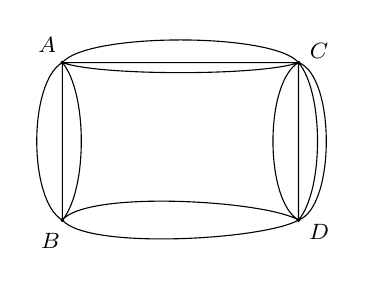
\begin{tikzpicture}[scale=1,line cap=round,line join=round,font=\footnotesize,>=stealth]
			\path
			(0,0) coordinate (A)
			(0,-2) coordinate (B)
			(3,-2) coordinate (D)
			(3,0) coordinate (C)
			;
			\draw (A) ..controls +(50:0.5) and +(130:0.5) ..(C) 
			(A) ..controls +(-150:0.5) and +(150:0.5) ..(B) 
			(B) ..controls +(-50:0.5) and +(-150:0.5) ..(D) 
			(D) ..controls +(50:0.5) and +(-50:0.5) ..(C) 
			(A)--(C) (A)--(B)
			(A) ..controls +(-20:0.5) and +(-160:0.5) ..(C) 
			(A) ..controls +(-50:0.5) and +(50:0.5) ..(B) 
			(B) ..controls +(50:0.5) and +(150:0.5) ..(D) 
			(D) ..controls +(50:0.5) and +(-50:0.5) ..(C) 
			(D) ..controls +(20:0.5) and +(-20:0.5) ..(C) 
			(D) ..controls +(150:0.5) and +(-150:0.5) ..(C)
			(C)--(D);
			\foreach \p/\g in {A/130,B/-120,C/30,D/-30} \draw[fill] (\p) circle(.5pt)node [shift={(\g:.3)}] {$\p$};
			
		\end{tikzpicture}
	}
	\loigiai{
		Có hai phương án để đi từ $A$ đến $D$.
		\begin{itemize}
			\item \textbf{Phương án 1:} Đi từ $A$ qua $B$ rồi đến $D$. Có $ 3 $ cách chọn đường đi từ $A$ đến $B$, có $ 2 $ cách chọn đường đi từ $B$ đến $D$. Theo quy tắc nhân, có $3 \cdot 2=6$ cách chọn đường đi từ $A$ qua $B$ rồi đến $D$.
			\item \textbf{Phương án 2:} Đi từ $A$ qua $C$ rồi đến $ D $. Có $ 3 $ cách chọn đường đi từ $A$ đến $C$, có $ 4 $ cách chọn đường đi từ $C$ đến $D$. Theo quy tắc nhân, có $3 \cdot 4=12$ cách chọn đường đi từ $A$ qua $C$ rồi đến $D$.
		\end{itemize}
		Áp dụng quy tắc cộng, có $6+12=18$ cách chọn đường đi từ $A$ đến $D$.}
\end{vd}

% #2973 | Archive/SP_KhoLatex/ID6_old/8D1.tex | mã gốc 1D2B1-1
\begin{bt}%[1D2B1-1]%[1D2B1-2]%[1D2B1-3]
	Trong một cái hộp có chứa $ 8 $ quả bóng màu trắng đánh số từ $ 1 $ đến $ 8 $; $ 10 $ quả bóng màu xanh đánh số từ $ 1 $ đến $ 10 $; $ 12 $ quả bóng màu cam đánh số từ $ 1 $ đến $ 12 $. Từ hộp này, có bao nhiêu cách
	\begin{enumerate}
		\item chọn ra một quả bóng?
		\item chọn ra ba quả bóng có màu khác nhau đôi một?
		\item chọn ra hai quả bóng có màu khác nhau đôi một?		
	\end{enumerate}
	\loigiai{
		\begin{enumerate}
			\item $8+10+12=30$. 
			\item $8 \cdot 10 \cdot 12=960$.
			\item  $8 \cdot 10+8 \cdot 12+10 \cdot 12=296$.
		\end{enumerate}
	}
\end{bt}

% #2974 | Archive/SP_KhoLatex/ID6_old/8D1.tex | mã gốc 1D2B1-2
\begin{bt}%[1D2B1-2]
	Ba lớp của một trường đang lên kế hoạch để đi dã ngoại, mỗi lớp có thể chọn một trong năm địa điểm. Có bao nhiêu kết quả có thể xảy ra về cách chọn địa điểm của ba lớp?
	\loigiai{
		Mỗi lớp có $ 5 $ cách chọn địa điểm.\\
		Theo quy tắc nhân, số cách chọn địa điểm của ba lớp là $5 \cdot 5 \cdot 5=125$.}
\end{bt}

% #2975 | Archive/SP_KhoLatex/ID6_old/8D1.tex | mã gốc 1D2B1-2
\begin{bt}%[1D2B1-2]
	\immini{Mã xác thực (OTP – One Time Password) do một ngân hàng gửi vào điện thoại của khách hàng cho mỗi lần giao dịch là một dãy $ 6 $ kí tự từ các chữ số từ $ 0 $ đến $ 9 $. Có thể tạo ra bao nhiêu mã xác thực khác nhau như vậy?	
	}{
		\begin{tabular}{|l|}
			\hline
			\texttt{Mã OTP xác thực giao } \\
			\texttt{dịch là $ 712892 $, hiệu}\\
			\texttt{lực trong 1 phút } $\ldots$\\ 
			\hline
	\end{tabular}}
	\loigiai{
		Có $ 10 $ cách chọn chữ số cho mỗi kí tự của mã xác nhận.\\
		Do đó theo quy tắc nhân, số mã xác nhận có thể tạo ra là $10^6=1000000$.}
\end{bt}

% #2976 | Archive/SP_KhoLatex/ID6_old/8D1.tex | mã gốc 1D2B1-2
\begin{bt}%[1D2B1-2]
	Tung một đồng xu $ 5 $ lần liên tiếp và ghi lại kết quả (ví dụ dùng kí hiệu $ SSNSN $ để chỉ kết quả $ 5 $ lần tung lần lượt là sấp, sấp, ngửa, sấp, ngửa). Có bao nhiêu kết quả khác nhau có thể xảy ra?
	\loigiai{
		Có thể coi việc tung đồng xu $ 5 $ lần liên tiếp là công việc gồm $ 5 $ công đoạn. Mỗi công đoạn có $ 2 $ phương án thực hiện, tương ứng đồng xu xuất hiện sấp hay ngửa. Do đó, theo quy tắc nhân, có $2 \cdot 2 \cdot 2 \cdot 2 \cdot 2=32$ kết quả có thể của việc tung đồng xu $ 5 $ lần liên tiếp.}
\end{bt}

% #2977 | Archive/SP_KhoLatex/ID6_old/8D1.tex | mã gốc 1D2B1-2
\begin{bt}%[1D2B1-2]
	\immini{Mã số nhân viên của một công ty có $ 4 $ kí tự, gồm một chữ cái đầu tiên (từ $ 6 $ chữ cái $ A $, $ B $, $ C $, $ D $, $ E $, $ F $) và tiếp theo là $ 3 $ chữ số (từ các chữ số $0, 1, \ldots ,9$). Công ty có thể tạo ra bao nhiêu mã số nhân viên theo cách này?	}{
		\begin{tikzpicture}
			\path
			(0,0) coordinate (A)
			($ (A)+(6,0) $) coordinate (B)
			($ (A)+(0,2.5) $) coordinate (D)
			($ (A)+(0,3.5) $) coordinate (M)
			($ (B) +(0,2.5) $) coordinate (C)
			($ (B) +(0,3.5) $) coordinate (N)
			($ (A)!0.8 !(D)$) coordinate (E)
			($ (B)!0.8 !(C)$) coordinate (F)
			($ (E)!0.45!(F) $) coordinate (E1)		
			($ (E)!0.55!(F) $) coordinate (F1)
			($ (M)!0.55!(N) $) coordinate (M1)
			($ (M)!0.45!(N) $) coordinate (N1)
			($ (E)!0.5!(F) $) coordinate (F11)
			($ (A)!0.5!(B) $) coordinate (F12)
			;
			\draw 
			(A)--(B)--(C)--(D)--cycle  (E1)--(F1)--(M1)--(N1)--cycle;
			\draw (0.2,0.8) --(1.5,0.8)--(1.5,1.8)--(.2,1.8)--cycle (1.7/2,2.6/2) node{Ảnh};
			\draw (1.1,0.4) node{\fbox{\tiny {Mã số:ABCD123}}} (F11)--(F12);
			\draw (4.5,2)node[below]{\tiny THẺ NHÂN VIÊN};
	\end{tikzpicture}}
	\loigiai{
		Có $ 6 $ cách chọn chữ cái cho kí tự đầu tiên.\\
		Với $ 3 $ kí tự tiếp theo, mỗi kí tự có $ 10 $ cách chọn từ 10 chữ số $0,1,2,\ldots,9$.\\
		Theo quy tắc nhân, công ty có thể tạo ra $6 \cdot 10 \cdot 10 \cdot 10=6000$ mã số nhân viên.}
\end{bt}

% #2978 | Archive/SP_KhoLatex/ID6_old/8D1.tex | mã gốc 1D2B1-2
\begin{bt}%[1D2B1-2]
	\immini{Có các con đường nối bốn ngôi làng $ A $, $ B $, $ C $, $ D $ như trong hình bên. Có bao nhiêu cách chọn đường đi khác nhau
		\begin{enumerate}
			\item  từ $ A $ qua $ B $ rồi đến $ D $? 
			\item  từ $ A $ đến $ D $?
		\end{enumerate} 
	}{
		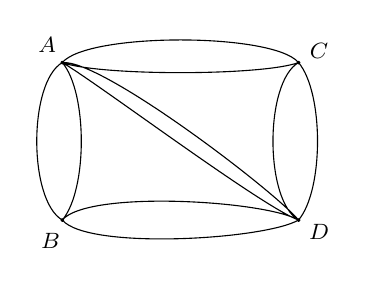
\begin{tikzpicture}[scale=1,line cap=round,line join=round,font=\footnotesize,>=stealth]
			\path
			(0,0) coordinate (A)
			(0,-2) coordinate (B)
			(3,-2) coordinate (D)
			(3,0) coordinate (C)
			;
			\draw (A) ..controls +(50:0.5) and +(130:0.5) ..(C) 
			(A) ..controls +(-150:0.5) and +(150:0.5) ..(B) 
			(B) ..controls +(-50:0.5) and +(-150:0.5) ..(D) 
			(D) ..controls +(50:0.5) and +(-50:0.5) ..(C) 
			(A) ..controls +(-20:0.5) and +(-160:0.5) ..(C) 
			(A) ..controls +(-50:0.5) and +(50:0.5) ..(B) 
			(B) ..controls +(50:0.5) and +(150:0.5) ..(D) 
			(D) ..controls +(50:0.5) and +(-50:0.5) ..(C) 
			%	(D) ..controls +(20:0.5) and +(-20:0.5) ..(C) 
			(D) ..controls +(150:0.5) and +(-150:0.5) ..(C)
			(A) ..controls +(5:0.5) and +(130:0.5) ..(D) 
			(A) ..controls +(-30:0.5) and +(160:0.5) ..(D) 
			;
			\foreach \p/\g in {A/130,B/-120,C/30,D/-30} \draw[fill] (\p) circle(.5pt)node [shift={(\g:.3)}] {$\p$};
			
		\end{tikzpicture}
	}
	\begin{note}
		Lưu ý: Mỗi đường đi qua mỗi ngôi làng nhiều nhất một lần.
	\end{note} 	
	\loigiai{
		\begin{enumerate}
			\item $ 2\cdot 2 =4 $.
			\item $2\cdot 2+2\cdot 2+2=10$.
	\end{enumerate}}
\end{bt}

% #2979 | Archive/SP_KhoLatex/ID6_old/8D1.tex | mã gốc 1D2B1-1
\begin{bt}%[1D2B1-1]
	\immini{Tung đồng thời hai con xúc xắc khác nhau và ghi lại số chấm xuất hiện trên mỗi con xúc xắc. Có bao nhiêu kết quả có thể xảy ra mà tổng số chấm xuất hiện trên hai mặt là bội của $ 5 $?	}{
		\begin{tikzpicture}	
			\tikzset{motcham/.pic={
					\begin{scope}[rounded corners=2mm]
						\def\a{2}
						\path(0,0)coordinate(A)++(-30:0.85*\a)coordinate(B)(1.5*\a,0)coordinate(C)($(A)+(C)-(B)$)coordinate(D);
						\path[shift={(0,\a)}](0,0)coordinate(A')++(-30:0.85*\a)coordinate(B')(1.5*\a,0)coordinate(C')($(A')+(C')-(B')$)coordinate(D');
						\fill[gray,draw=gray](A)--(A')--(D')--(C')--(C)--(B)--cycle;
						\draw[fill=gray!30,draw=gray](B)--(C)--(C')--(B')--cycle (A')--(B')--(C')--(D')--cycle (A)--(A')--(B')--(B)--cycle;
						\fill[ball color=red,yscale=0.5,draw=red!30]($(A')!0.5!(C')$)circle(0.25*\a)($(A')!0.5!(C')$)circle(0.25*\a);
						\path($(A')!0.5!(B')$)coordinate(M')($(A)!0.5!(B)$)coordinate(M);
						\fill[ball color=red,yslant=-0.3,,draw=red!30]($(M)!1/3!(M')$)circle(0.125*\a)($(M)!2/3!(M')$)circle(0.125*\a);
						\path($(B')!1/3!(C')$)coordinate(N')($(B) !1/3!(C)$)coordinate(N)($(B')!2/3!(C')$)coordinate(P')($(B)!2/3!(C)$)coordinate(P);
						\fill[ball color=red,yslant=0.3,draw=red!30]($(N)!1/3!(N')$)circle(0.1*\a)($(N)!2/3!(N')$)circle(0.1*\a)($(P)!1/3!(P')$)circle(0.1*\a)($(P)!2/3!(P')$)circle(0.1*\a);
					\end{scope}
			}}
			\path(0,0)pic{motcham};
			\path (3.5,0) pic{motcham};
	\end{tikzpicture}}
	\loigiai{
		Ta viết $(a,b)$ để kí hiệu kết quả số chấm xuất hiện trên hai con xúc xắc lần lượt là $a$ và $b$. \\
		Ta có $2 \leq a+b \leq 12$ nên $a+b$ là bội của $ 5 $ khi $a+b=5$ hoặc $a+b=10$.
		\begin{itemize}
			\item Trường hợp $a+b=5$ gồm các kết quả: $(1,4),(2,3),(3,2),(4,1)$.\\ Trường hợp này có $ 4 $ kết quả.
			\item Trường hợp $a+b=10$ bao gồm các kết quả: $(4,6),(5,5),(6,4)$.\\ Trường hợp này có $ 3 $ kết quả.
		\end{itemize} 
		Vậy có $4+3=7$ kết quả có thể xảy ra mà tổng số chấm xuất hiện trên hai con xúc xắc là bội của $ 5 $.}
\end{bt}

% #2980 | Archive/SP_KhoLatex/ID6_old/8D1.tex | mã gốc 1D2B1-2
\begin{bt}%[1D2B1-2]
	\immini{	Một khoá tổ hợp với đĩa quay có $ 40 $ vạch số (xem hình bên). Mật mã của khoá là một dãy gồm $ 3 $ số, kí hiệu là $a-b-c$, mỗi số là một số tự nhiên từ $ 0 $ đến $ 39 $. Để mở khoá, cần quay mặt số ngược chiều kim đồng hồ cho đến khi điểm mốc gặp vạch số $a$ lần thứ ba, rồi quay mặt số theo chiều ngược lại cho đến khi điểm mốc gặp vạch số $b$ lần thứ hai, cuối cùng quay mặt số ngược chiều kim đồng hồ cho đến khi điểm mốc gặp vạch số $c$ lần đầu tiên. Nếu $a$, $b$, $c$ phải khác nhau đôi một, thì có bao nhiêu cách chọn mật mã cho khoá tổ hợp trên?	}{
		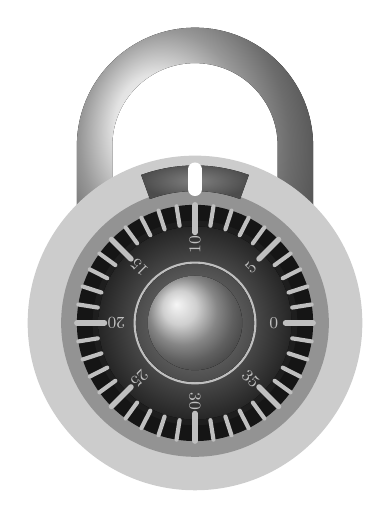
\begin{tikzpicture}[font=\footnotesize, line join=round, line cap=round, >=stealth,scale=0.5]
			\begin{scope}[transform shape]
				\tikzset{Khoa-mat-ma/.pic={
						\def\R{3}
						\def\g{9}
						\fill[ball color=gray!30](-\R,0)--++(90:1.5*\R)arc(180:0:\R)--(\R,0)--(0.7*\R,0)--++(90:1.5*\R)arc(0:180:0.7*\R)--(-0.7*\R,0)--cycle;
						\fill[gray!40](0,0)circle(\R+1.25);
						\draw[gray,line width=4mm,opacity=0.75](0,0)circle(\R);
						\fill[opacity=0.85](0,0)circle(\R);
						\fill[outer color=black!85](0,0)circle(\R-0.55);
						\fill[gray!50](0,0)circle(0.52*\R);
						\fill[outer color=black!70](0,0)circle(0.5*\R);
						\fill[ball color=gray!50](0,0)circle(0.4*\R);
						\fill[outer color=black!70](70:{\R+1})arc(70:110:{\R+1})--(110:\R+0.35)arc(110:70:{\R+0.35});
						\draw[white,line width=5pt](90:\R+0.4)--++(90:0.5);
						\foreach \i in{0,9,...,354}{
							\pgfmathsetmacro{\k}{int(mod(\i,5))}
							\pgfmathsetmacro{\m}{int(\i/9)}
							\draw[white!50!gray,line width=1.5pt](\i:\R)--++(180+\i:0.5);
							\ifnum \k=0
							\draw[white!50!gray,line width=2pt](\i:\R)--++(180+\i:0.7);
							\path(\i*\g:\R)++(180+\i*\g:1)node[scale=1.5,rotate=\i]{\color{white!50!gray}$\m$};
							\fi
				}}}
				\path(0,0)pic{Khoa-mat-ma};
			\end{scope}
	\end{tikzpicture}}
	\loigiai{
		Có $ 40 $ cách chọn số $a$ từ các số từ $ 0 $ đến $ 39 $. Tiếp theo, có $ 39 $ cách chọn số $b$ từ $ 39 $ số còn lại. Cuối cùng, có $ 38 $ cách chọn số $c$ từ $ 38 $ số còn lại. Áp dụng quy tắc nhân, ta có $40\cdot 39\cdot 38 = 59280$ cách chọn mật mã cho khoá.}
\end{bt}

% #3017 | Archive/SP_KhoLatex/ID6_old/10D8-25.tex | mã gốc 1D2B3-1
\begin{vd}%[1D2B3-1]
	Khai triển $\left(x+3\right)^4$.
	\loigiai{Áp dụng công thức khai triển của $\left(a+b\right)^4$ với $a=x,$ $b=3,$ ta có\\
	$\left(x+3\right)^4=x^4+4x^3\cdot3+6x^2\cdot3^2+4x\cdot3^3+3^4
	=x^4+12x^3+54x^2+108x+81$.\\}
\end{vd}

% #3018 | Archive/SP_KhoLatex/ID6_old/10D8-25.tex | mã gốc 1D2K3-1
\begin{vd}%[1D2K3-1]
	Hãy sử dụng ba hạng tử đầu tiên trong khai triển của $\left(3-0,02\right)^5$ để tính giá trị gần đúng của $2,98^5$. Xác định sai số tuyệt đối của giá trị gần đúng nhận được.
	\loigiai{Ta có $2,98^5=\left(3-0,02\right)^5$.\\
	Sử dụng công thức khai triển $\left(a+b\right)^5$, áp dụng cho $a=3,$ $b=-0,02,$ ta thu được:\\
	$2,98^5=\left(3-0,02\right)^5=3^5+5\cdot3^4\cdot(-0,02)+10\cdot3^3\cdot\left(-0,02\right)^2+...$\\
	$=243-405\cdot0,02+270\cdot0,0004+...$\\
	$=243-8,1+0,108+...$\\
	$\approx 235,008$.\\
	Bằng máy tính, ta kiểm được rằng giá trị đúng là $235,0072823968$. Như vậy, sai số tuyệt đối của giá trị gần đúng nhận được trên đây là\\
	$\mid235,0072823968-235,008\mid=0,0007176032$.\\}
\end{vd}

% #3019 | Archive/SP_KhoLatex/ID6_old/10D8-25.tex | mã gốc 1D2B3-1
\begin{bt}%[1D2B3-1]
	Khai triển các đa thức
	\begin{listEX}[4]
		\item $\left(x-2\right)^4;$
		\item $\left(x+2\right)^5;$
		\item $\left(2x+3y\right)^4;$
		\item $\left(2x-y\right)^5.$
	\end{listEX}
	\loigiai{
		\begin{listEX}[1]
			\item $\left(x-2\right)^4=x^4+4x^3\cdot(-2)+6x^2\cdot\left(-2\right)^2+4x\cdot\left(-2\right)^3+\left(-2\right)^4$\\
			$=x^4-8x^3+24x^2-32x+16$.
			\item $\left(x+2\right)^5=x^5+5x^4\cdot2+10x^3\cdot2^2+10x^2\cdot2^3+5x\cdot2^4+2^5$\\
			$=x^5+10x^4+40x^3+80x^2+80x+32$.
			\item $\left(2x+3y\right)^4=\left(2x\right)^4+4\cdot\left(2x\right)^3\cdot3y+6\cdot\left(2x\right)^2\cdot\left(3y\right)^2+4\cdot2x\cdot\left(3y\right)^3+\left(3y\right)^4$\\
			$=16x^4+96x^3y+216x^2y^2+216xy^3+81y^4$.
			\item $\left(2x-y\right)^5=\left(2x\right)^5+5\cdot\left(2x\right)^4\cdot(-y)+10\cdot\left(2x\right)^3\cdot\left(-y\right)^2$\\
			$+10\cdot\left(2x\right)^2\cdot\left(-y\right)^3+5\cdot2x\cdot\left(-y\right)^4+\left(-y\right)^5$\\
			$=32x^5-80x^4y+80x^3y^2-40x^2y^3+10xy^4-y^5$.
		\end{listEX}
}
\end{bt}

% #3020 | Archive/SP_KhoLatex/ID6_old/10D8-25.tex | mã gốc 1D2B3-2
\begin{bt}%[1D2B3-2]
	Trong khai triển của $\left(5x-2\right)^5$, số mũ của $x$ được sắp xếp theo lũy thừa tăng dần, hãy tìm hạng tử thứ hai.
	\loigiai{Áp dụng công thức khai triển của $\left(a+b\right)^5$ với $a=5x,$ $b=-2,$ ta có\\
	$\left(5x-2\right)^5=\left(5x\right)^5+5\cdot\left(5x\right)^4\cdot(-2)+10\cdot\left(5x\right)^3\cdot\left(-2\right)^2
	+10\cdot\left(5x\right)^2\cdot\left(-2\right)^3+5\cdot5x\cdot\left(-2\right)^4+\left(-2\right)^5$\\
	$=-32+400x-2000x^2+5000x^3- 6250x^4+3125x^5$.\\
	Vậy, số hạng thứ hai trong khai triển theo số mũ tăng dần của $x$ là $400x$.\\}
\end{bt}

% #3021 | Archive/SP_KhoLatex/ID6_old/10D8-25.tex | mã gốc 1D2K3-1
\begin{bt}%[1D2K3-1]
	Hãy sử dụng ba số hạng đầu tiên trong khai triển của $\left(1+0,03\right)^4$ để tính giá trị gần đúng của $1,03^4$. Xác định sai số tuyệt đối.
	\loigiai{Ta có:\\
	$1,03^4=(1+0,03)^4=1^4+4\cdot1^3\cdot0,03+6\cdot1^2\cdot(0,03)^2+...$\\
	$=1+0,12+0,0054+...\approx1,1254$.\\
	Mặt khác, ta tính được giá trị đúng, chẳng hạn bằng máy tính,\\
	$1,03^4=1,12550881$.\\
	Như vậy, sai số tuyệt đối của giá trị gần đúng nhận được so với giá trị đúng là:\\
	$\mid 1,1254-1,12550881 \mid=0,00010881$.\\}
\end{bt}

% #3022 | Archive/SP_KhoLatex/ID6_old/10D8-25.tex | mã gốc 1D2B3-2
\begin{bt}%[1D2B3-2]
	Xác định hạng tử không chứa $x$ trong khai triển của $\left(x+\dfrac{2}{x}\right)^4$.\\
	\loigiai{Ta có:\\
	$\left(x+\dfrac{2}{x}\right)^4=x^4+4x^3\cdot\dfrac{2}{x}+6x^2\cdot\left(\dfrac{2}{x}\right)^2+4x\cdot\left(\dfrac{2}{x}\right)^3+\left(\dfrac{2}{x}\right)^4$\\
	$=x^4+8x^2+24+\frac{32}{x^2}+\dfrac{16}{x^4}$.\\
	Vậy, hạng tử không chứa $x$ là $24$.\\}
\end{bt}

% #3023 | Archive/SP_KhoLatex/ID6_old/10D8-25.tex | mã gốc 1D2K3-1
\begin{bt}%[1D2K3-1]
	Khai triển $\left(z^2+1+\dfrac{1}{z}\right)^4$.
	\loigiai{Trước hết, ta sử dụng công thức khai triển của $\left(a+b\right)^4$ với $a=z^2+1$ và $b=\dfrac{1}{z}$, sau đó, ta sử dụng các công thức khai triển của $\left(a+b\right)^4,$ $\left(a+b\right)^3,$ $\left(a+b\right)^2$ với $a=z^2,$ $b=1$ để có:\\
	$\left(z^2+1+\dfrac{1}{z}\right)^4=\left(z^2+1\right)^4+4\left(z^2+1\right)^3\cdot\dfrac{1}{z}+6\left(z^2+1\right)^2\cdot\dfrac{1}{z^2}+4\left(z^2+1\right)\cdot\dfrac{1}{z^3}+\dfrac{1}{z^4}$\\
	$=\left(z^8+4z^6+6z^4+4z^2+1\right)+4\left(z^6+3z^4+3z^2+1\right)\cdot\dfrac{1}{z}$\\
	$+6\left(z^4+2z^2+1\right)\cdot\dfrac{1}{z^2}+4\left(z^2+1\right)\cdot\dfrac{1}{z^3}+\dfrac{1}{z^4}$\\
	$=z^8+4z^6+4z^5+6z^4+12z^3+10z^2+12z+13+\dfrac{8}{z}+\dfrac{6}{z^2}+\dfrac{4}{z^3}+\dfrac{1}{z^4}$.\\}
\end{bt}

% #3024 | Archive/SP_KhoLatex/ID6_old/1D2K5-2.tex | mã gốc 1D2K5-2
\begin{ex}%[Đề thi HK1, THPT Nguyễn Du, THPCM năm học 2018-2019]%[Nguyễn Quang Dũng, dự án 11EX-HK1-1819]%[1D2K5-2]
Trước tết nguyên đán Kỷ Hợi năm $2019$, Ban Giám Hiệu Trường THPT Nguyễn Du sẽ tổ chức chương trình \lq\lq \textbf{Tình ca mùa xuân} \rq\rq\ tại trường. Ban Giám Hiệu dự định mời các ca sĩ được học sinh yêu thích gồm: Mỹ Tâm, Đông Nhi, Hồ Ngọc Hà, Hương Tràm, Bích Phương, Tóc Tiên (6 nữ ca sĩ), Đan Trường, Đàm Vĩnh Hưng, Noo Phước Thịnh, Hà Anh Tuấn ($4$ nam ca sĩ). Hiện tại Ban Giám Hiệu đã mời được $2$ ca sĩ là Mỹ Tâm và Đan Trường, trong các ca sĩ còn lại Ban Giám Hiệu chọn ngẫu nhiên $3$ ca sĩ. Tính xác suất để Ban Giám Hiệu chọn được ít nhất hai nữ ca sĩ cho buổi biểu diễn.\dapso{$\mathrm{P}\left(A\right)=\dfrac{55}{56}$.}
\loigiai{
Các ca sĩ có thể được mời gồm có $6$ nữ ca sĩ, $4$ nam ca sĩ. Do đã chọn được hai ca sĩ, nên mỗi cách chọn $3$ ca sĩ ứng với một tổ hợp chập $3$ của $8$ ca sĩ còn lại.\\
Suy ra số phần tử của không gian mẫu là $n\left(\Omega\right)=\mathrm{C}_8^3=56$.\\
Gọi $A$ là biến cố \lq\lq Có ít nhất hai nữ ca sĩ được chọn cho buổi biểu diễn\rq\rq.\\
Trong $3$ ca sĩ sẽ được chọn, để xảy ra biến cố $A$ ta có các trường hợp
\begin{itemize}
\item Trường hợp $1$: Đúng một nữ ca sĩ được chọn, có $\mathrm{C}_5^1\times\mathrm{C}_3^2$ cách chọn.
\item Trường hợp $2$: Đúng $2$ nữ ca sĩ được chọn, có $\mathrm{C}_5^2\times\mathrm{C}_3^1$ cách chọn.
\item Trường hợp $3$: Cả $3$ ca sĩ còn lại đều là nữ, có $\mathrm{C}_5^3$ cách chọn.
\end{itemize}
Số phần tử của biến cố $A$ là $n(A)=55$.\\
Xác suất của biến cố $A$ là $\mathrm{P}\left(A\right)=\dfrac{n(A)}{n(\Omega)}=\dfrac{55}{56}$.\\
$\bullet$ \textbf{Nhận xét:} \textit{Bài này để đếm số phần tử của $A$ ta có thể đếm số phần tử của $\overline{A}$, $n(\overline{A})=\mathrm{C}_3^3$ (cả $3$ ca sĩ còn lại đều là nam).}}
\end{ex}

% #3028 | Archive/SP_KhoLatex/ID6_old/10XSOTC.tex | mã gốc 1D2K5-2
\begin{bt}%[Tex hóa SGK CD-CT,T7/22, Nguyễn Trung Kiên]%%[1D2K5-2]%Bài 1
	\immini
	{Trên bàn có một tấm bìa hình tròn được chia thành $10$ hình quạt bằng nhau và được đánh số từ $1$ đến $10$ như Hình $ 4 $. Cường quay mũi tên ở tâm $ 3 $ lần và quan sát xem khi mỗi lần dừng lại nó chỉ vào ô số mấy. Tính xác suất của các biến cố sau:
		\begin{enumerate}
			\item $A$: \lq\lq Cả $3$ lần mũi tên đều chỉ vào ô ghi số lẻ\rq\rq.
			\item $B$: \lq\lq Tích $3$ số mũi tên chỉ vào là số chia hết cho $5$\rq\rq.	
	\end{enumerate}}
	{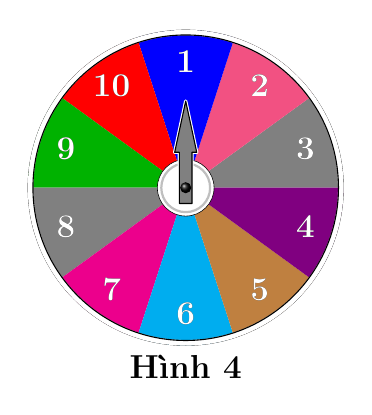
\begin{tikzpicture}[scale=1,font=\footnotesize,line join=round,line cap=round,>=stealth]
			\draw[black] (0,0) circle(2);
			\foreach \t/\c in {1/gray,2/yellow!30!magenta,3/blue,4/red,5/green!70!black,6/gray,7/magenta,8/cyan,9/brown,10/violet}
			\fill[\c] (0,0)--(\t*36-36:2) arc(\t*36-36:\t*36:2)--cycle;
			\draw[white,line width=2.pt] (0,0) circle(1.97);
			\draw[] (0,0) circle(1.94);
			\draw[fill=white, very thin] (0,0) circle(0.36);
			\draw[gray!50,fill=white, thick] (0,0) circle(0.31);
			\draw[white,very thick] (-0.08,-0.2)--(-0.08,0.45)--(-0.14,0.45)--(0,1.1)--(0.14,0.45)--(0.08,0.45)--(0.08,-0.2)--cycle;
			\draw[fill=gray] (-0.08,-0.2)--(-0.08,0.45)--(-0.14,0.45)--(0,1.1)--(0.14,0.45)--(0.08,0.45)--(0.08,-0.2)--cycle;
			\shade[ball color=black] (0,0) circle(2pt);
			\foreach \t in {1,2,...,10}{
				\node at (126-\t*36:1.6){\fontsize{13}{0}\selectfont\color{black}\bf\t};
				\node at (126-\t*36:1.6){\fontsize{12}{0}\selectfont\color{white}\bf\t};
			}
			\node at (-90:2)[below]{\fontsize{12}{0}\selectfont\textbf{Hình 4}};
	\end{tikzpicture}}
	\loigiai
	{Không gian mẫu của phép thử \lq\lq Cường quay mũi tên ở tâm $3$ lần\rq\rq\, có số phần tử là $n(\Omega)=10^3$.\\
		\begin{enumerate}
			\item Biến cố $A$: \lq\lq Cả $3$ lần mũi tên đều chỉ vào ô ghi số lẻ\rq\rq\, có số các kết quả thuận lợi là $n(A)=5^3$.\\
			Vậy xác suất của biến cố $A$ là $\mathrm{P}(A)=\dfrac{n(A)}{n(\Omega)}=\dfrac{5^3}{10^3} = \dfrac{1}{8}$.
			\item Xét biến cố $B$: \lq\lq Tích $3$ số mũi tên chỉ vào là số chia hết cho $5$\rq\rq. \\
			Biến cố  $\overline{B}$: \lq\lq Tích $3$ số mũi tên chỉ vào là số không chia hết cho $5$\rq\rq. Khi đó các lần quay mũi tên đều không chỉ vào số $5$ và số $10$, do đó số các kết quả thuận lợi của biến cố $\overline{B}$ là $n\left(\overline{B}\right)=8^3$.\\
			Vậy xác suất của biến cố $B$ là
			$$\mathrm{P}(B)=1-\mathrm{P}\left(\overline{B}\right) = 1-\dfrac{n\left(\overline{B}\right)}{n(\Omega)} = 1-\dfrac{8^3}{10^3} = \dfrac{61}{125}.$$
	\end{enumerate}}
\end{bt}

% #3029 | Archive/SP_KhoLatex/ID6_old/10XSOTC.tex | mã gốc 1D2B5-2
\begin{bt}%[Tex hóa SGK CD-CT,T7/22, Nguyễn Trung Kiên]%%[1D2B5-2]%Bài 2
	Mật khẩu mở máy tính của An gồm $8$ kí tự, trong đó $2$ kí tự đầu là chữ số, $6$ kí tự sau là các chữ cái thuộc tập hợp $\{A;B;C;D\}$. Không may An quên mất $3$ kí tự đầu tiên. An chọn ra $2$ chữ số và một chữ cái thuộc tập hợp trên một cách ngẫu nhiên và thử mở máy tính. Tính xác suất để An mở được máy tính.
	\loigiai
	{Số kết quả có thể xảy ra của việc nhập theo thứ tự $2$ chữ số và một chữ cái thuộc tập $\{A;B;C;D\}$ là $n(\Omega)=10\cdot 10\cdot 4 = 400$.\\
		Do chỉ có $1$ kết quả là mật khẩu nên xác suất để An mở được máy tính là $\mathrm{P}=\dfrac{1}{400}$.}
\end{bt}

% #3030 | Archive/SP_KhoLatex/ID6_old/10XSOTC.tex | mã gốc 1D2B5-2
\begin{bt}%[Tex hóa SGK CD-CT,T7/22, Nguyễn Trung Kiên]%%[1D2B5-2]%Bài 3
	Tổ $3$ có $6$ bạn là Hoà, Hiền, Hiệp, Hương, Thành và Khánh. Chọn ngẫu nhiên $2$ bạn trong tổ. Hãy tính xác suất của các biến cố:\\
	$A$: \lq\lq Tên của hai bạn được chọn đều bắt đầu bằng chữ cái H\rq\rq;\\
	$B$: \lq\lq Tên của ít nhất một bạn được chọn có chứa dấu huyền\rq\rq;\\
	$C$: \lq\lq Hoà được chọn còn Hiền không được chọn\rq\rq.
	\loigiai
	{Phép thử \lq\lq Chọn ngẫu nhiên $2$ bạn trong tổ\rq\rq\, có số phần tử của không gian mẫu là $n(\Omega)=\mathrm{C}_6^2=15$.
		\begin{itemize}
			\item Xét biến cố $A$: \lq\lq Tên của hai bạn được chọn đều bắt đầu bằng chữ cái H\rq\rq. Do có $4$ bạn có tên bắt đầu bằng chữ H nên số các kết quả thuận lợi cho $A$ là $n(A)=\mathrm{C}_4^2=6$.\\
			Vậy xác suất của biến cố $A$ là $\mathrm{P}(A)=\dfrac{6}{15}=\dfrac{2}{5}$.
			\item Xét biến cố $B$: \lq\lq Tên của ít nhất một bạn được chọn có chứa dấu huyền\rq\rq. Khi đó biến cố $\overline{B}$: \lq\lq Hai bạn được chọn tên không có chứa dấu huyền\rq\rq. Do có $3$ bạn tên không chứa dấu huyền nên số các kết quả thuận lợi cho $\overline{B}$ là $n\left(\overline{B}\right)=\mathrm{C}_3^2=3$.\\
			Vậy xác suất của biến cố $B$ là $\mathrm{P}(B)=1-\mathrm{P}\left(\overline{B}\right) = 1-\dfrac{3}{15} = \dfrac{4}{5}$.
			\item Xét biến cố $C$: \lq\lq Hoà được chọn còn Hiền không được chọn\rq\rq. Khi đó ta chọn Hòa và $1$ trong $4$ bạn còn lại không phải Hiền nên số các kết quả thuận lợi cho $C$ là $n(C)=1\cdot4=4$.\\
			Vậy xác suất của biến cố $C$ là $\mathrm{P}(C)=\dfrac{4}{15}$.
	\end{itemize}}
\end{bt}

% #3031 | Archive/SP_KhoLatex/ID6_old/10XSOTC.tex | mã gốc 1D2B5-2
\begin{bt}%[Tex hóa SGK CD-CT,T7/22, Nguyễn Trung Kiên]%%[1D2B5-2]%Bài 4
	Một hộp có $5$ lá thăm cùng loại được đánh số $2;4;6;8;10$. Lấy ra ngẫu nhiên từ hộp $2$ lá thăm. Tính xác suất của các biến cố sau:\\
	$A$: \lq\lq Tổng các số ghi trên hai lá thăm bằng $11$\rq\rq;\\
	$B$: \lq\lq Tích các số ghi trên hai lá thăm là số tròn chục\rq\rq.
	\loigiai
	{Phép thử \lq\lq Lấy ngẫu nhiên từ hộp $2$ lá thăm\rq\rq\, có số phần tử của không gian mẫu là $n(\Omega)=\mathrm{C}_5^2=10$.
		\begin{itemize}
			\item Xét biến cố $A$: \lq\lq Tổng các số ghi trên hai lá thăm bằng $11$\rq\rq. Do cả $5$ lá thăm mang số chẵn nên không thể xảy ra khả năng tổng các số ghi trên hai lá thăm bằng $11$, suy ra $n(A)=0$.\\
			Vậy xác suất của biến cố $A$ là $\mathrm{P}(A)=0$.
			\item Xét biến cố $B$: \lq\lq Tích các số ghi trên hai lá thăm là số tròn chục\rq\rq. Khi đó trong $2$ thăm lấy ra phải có $1$ thăm ghi số $10$. Do đó số các kết quả thuận lợi của biến cố $B$ là $n(B)=4$.\\
			Vậy xác suất của biến cố $B$ là $\mathrm{P}(B)=\dfrac{4}{10}=\dfrac{2}{5}$. 
	\end{itemize}}
\end{bt}

% #3032 | Archive/SP_KhoLatex/ID6_old/10XSOTC.tex | mã gốc 1D2B5-2
\begin{bt}%[Tex hóa SGK CD-CT,T7/22, Nguyễn Trung Kiên]%%[1D2B5-2]%Bài 5
	Doanh nghiệp $A$ chọn ngẫu nhiên $2$ tháng trong năm $2021$ để tri ân khách hàng. Doanh nghiệp $B$ cũng chọn ngẫu nhiên $1$ tháng trong năm đó để tri ân khách hàng. Tính xác suất của biến cố \lq\lq Hai doanh nghiệp tri ân khách hàng cùng một tháng trong năm\rq\rq.
	\loigiai
	{Số các kết quả có thể xảy ra là $n(\Omega)=\mathrm{C}_{12}^2 \cdot \mathrm{C}_{12}^1 = 792$.\\
		Gọi $A$ là biến cố \lq\lq Hai doanh nghiệp tri ân khách hàng cùng một tháng trong năm\rq\rq. Khi đó $\overline{A}$ là biến cố \lq\lq Hai doanh nghiệp tri ân khách hàng không cùng một tháng trong năm\rq\rq.\\
		Số các kết quả thuận lợi cho $\overline{A}$ là $n\left(\overline{A}\right)=\mathrm{C}_{12}^2 \cdot \mathrm{C}_{10}^1 = 660$.\\
		Vậy xác suất của biến cố $A$ là $\mathrm{P}(A)= 1-\mathrm{P}\left(\overline{A}\right) = 1-\dfrac{660}{792}=\dfrac{1}{6}$.}
\end{bt}

% #3033 | Archive/SP_KhoLatex/ID6_old/10XSOTC.tex | mã gốc 1D2B5-2
\begin{bt}%[Tex hóa SGK CD-CT,T7/22, Nguyễn Trung Kiên]%%[1D2B5-2]%Bài 6
	Lớp học của hai bạn Hà và Giang có $32$ học sinh. Cô giáo chia các bạn vào $4$ tổ, mỗi tổ có $8$ học sinh một cách ngẫu nhiên. Tính xác suất của các biến cố \lq\lq Hà và Giang được xếp ở hai tổ khác nhau\rq\rq.
	\loigiai
	{Phép thử \lq\lq Chia $32$ học sinh vào $4$ tổ , mỗi tổ có $8$ học sinh một cách ngẫu nhiên\rq\rq. Số phần tử của không gian mẫu là $n(\Omega)=\mathrm{C}_{32}^8 \mathrm{C}_{24}^8 \mathrm{C}_{16}^8 \mathrm{C}_8^8$.\\
		Gọi $A$ là biến cố \lq\lq Hà và Giang được xếp ở hai tổ khác nhau\rq\rq. Ta có $\overline{A}$ là biến cố \lq\lq Hà và Giang được xếp ở cùng một tổ\rq\rq, khi đó Hà và Giang có $4$ cách xếp vào một trong các tổ, có $\mathrm{C}_{30}^6$ cách chọn $6$ bạn vào tổ có Hà và Giang, $\mathrm{C}_{24}^8\mathrm{C}_{16}^8\mathrm{C}_8^8$ cách chọn các học sinh vào các tổ còn lại. Do đó $n\left(\overline{A}\right) = \mathrm{C}_{30}^6 \mathrm{C}_{24}^8 \mathrm{C}_{16}^8 \mathrm{C}_8^8$.\\
		Vậy xác suất của biến cố $A$ là   
		$$\mathrm{P}(A)= 1-\mathrm{P}\left(\overline{A}\right) = 1-\dfrac{4\mathrm{C}_{30}^6\mathrm{C}_{24}^8\mathrm{C}_{16}^8\mathrm{C}_8^8}{\mathrm{C}_{32}^8\mathrm{C}_{24}^8\mathrm{C}_{16}^8\mathrm{C}_8^8}=1-\dfrac{4\mathrm{C}_{30}^6}{\mathrm{C}_{32}^8}=\dfrac{24}{31}.$$}
\end{bt}

% #3034 | Archive/SP_KhoLatex/ID6_old/10XSOTC.tex | mã gốc 1D2K5-2
\begin{bt}%[Tex hóa SGK CD-CT,T7/22, Nguyễn Trung Kiên]%%[1D2K5-2]%Bài 7
	Một hộp chứa $2$ quả bóng xanh và một số quả bóng trắng. Lấy ra ngẫu nhiên $2$ quả bóng từ hộp. Biết rằng xác suất chọn được $2$ quả bóng khác màu là $\dfrac{10}{21}$.
	\begin{enumerate}
		\item Tính xác suất $2$ quả bóng lấy ra có cùng màu.
		\item Hỏi trong hộp có bao nhiêu quả bóng?
	\end{enumerate}
	\loigiai
	{\begin{enumerate}
			\item Gọi $A$ là biến cố \lq\lq $2$ quả bóng lấy ra cùng màu\rq\rq. Khi đó $\overline{A}$ là biến cố \lq\lq $2$ quả bóng lấy ra khác màu\rq\rq.\\
			Xác suất của biến cố $A$ là $\mathrm{P}(A)=1-\mathrm{P}\left(\overline{A}\right)=1-\dfrac{10}{21}=\dfrac{11}{21}$.
			\item Gọi $k$ là số quả bóng trắng trong hộp $\left(k \in\mathbb{N}^*\right)$. Phép thử \lq\lq Lấy ra ngẫu nhiên $2$ quả bóng từ hộp\rq\rq\, có số phần tử của không gian mẫu là $n(\Omega)=\mathrm{C}_{k+2}^2$.\\
			Biến cố $A$: \lq\lq $2$ quả bóng lấy ra khác màu\rq\rq\, có số các kết quả thuận lợi là $n(A)=\mathrm{C}_2^1\mathrm{C}_k^1=2k$.\\
			Theo bài ra xác suất chọn được $2$ quả bóng khác màu là $\dfrac{10}{21}$ nên ta có
			$$\dfrac{2k}{\mathrm{C}_{k+2}^2}=\dfrac{10}{21} \Leftrightarrow \dfrac{4k}{(k+1)(k+2)}=\dfrac{10}{21} \Leftrightarrow 10k^2-54k+20=0 \Leftrightarrow \hoac{&k=5\text{ (thỏa mãn)}\\&k=\dfrac{2}{5}\text{ (loại).}}$$
			Vậy trong hộp có $7$ quả bóng.
	\end{enumerate}}
\end{bt}

% #3043 | Archive/SP_KhoLatex/ID6_old/0-HK1-19-ChuyenLuongTheVinh-TN-2223.tex | mã gốc 1D2G5-2
\begin{bt}%[Đề kiểm tra HK1 môn Toán 10 trường THPT Chuyên Lương Thế Vinh]%[Lê Minh Thiện Anh, 10EX-HK1-2223]%[1D2G5-2]
	Có $12$ học sinh, trong đó có $9$ nam và $3$ nữ. Giáo viên chia $12$ học sinh trên thành $3$ nhóm để làm bài tập nhóm, biết rằng bài tập được giao ở mỗi nhóm là khác nhau từng đôi một.
	\begin{enumerate}
	\item Tính số cách chia sao cho mỗi nhóm có $3$ học sinh nam và $1$ học sinh nữ.
	\item Tính xác suất sao cho có ít nhất một nhóm không có học sinh nữ nào.
	\end{enumerate}
	\loigiai{
		\begin{enumerate}
		\item Nhóm 1 có $\mathrm{C}_3^1\cdot \mathrm{C}_9^3 = 252$ cách.\\
		Lúc đó còn lại $2$ nữ, $6$ nam, nhóm thứ 2 có $\mathrm{C}_2^1\cdot \mathrm{C}_6^3 = 40$ cách chọn.\\
		Cuối cùng còn $4$ người là một nhóm có $1$ cách.\\
		Theo quy tắc nhân thì có $252\cdot 40\cdot 1= 10080$ cách.
		\item Có $12$ học sinh, chọn ra $4$ học sinh thì có 
		$\mathrm{C}_{12}^4$ cách.\\
		Còn lại $8$ học sinh, chọn tiếp ra $4$ học sinh thì có 
		$\mathrm{C}_{8}^4$, còn lại $4$ học sinh là nhóm cuối.\\
		Vậy không gian mẫu $n(\Omega)=\mathrm{C}_{12}^4\cdot \mathrm{C}_{8}^4\cdot1=34650$.\\
		Gọi $A$ là biến cố \lq\lq có ít nhất một nhóm không có học sinh nữ nào\rq\rq.\\
		$\overline{A}$ là biến cố \lq\lq cả ba nhóm đều có nữ\rq\rq.\\ 
		Ta có $n(\overline{A})=252\cdot 40\cdot 1= 10080$.\\
		Vậy xác suất cần tìm là $P(A)=1-P(\overline{A})=1-\dfrac{10080}{34650}=\dfrac{39}{55}$.
		\end{enumerate}
	}
\end{bt}

% #3082 | Archive/SP_KhoLatex/ID6_old/0-HK1-3-LeHongPhong-TN-TL-2223.tex | mã gốc 1D2B1-2
\begin{bt}%[Đề HK1, trường THPT Chuyên Lê Hồng Phong, Nam Định]%[TVN-361, 10EX-HK1-2223 (đợt 2)]%%[1D2B1-2]
	Từ các chữ số $0;1;2;3;4;5;6;7;8$, lập được bao nhiêu số tự nhiên có $3$ chữ số?
	\loigiai{
		Xét số tự nhiên dạng $\overline{abc}$ với $a \neq 0$, $a,b,c \in \{0;1;2;3;4;5;6;7;8\}$.\\
		Số cách chọn $a,b,c$ theo thứ tự là $8,9,9$ nên có $8\cdot 9\cdot 9=648$ số thoả mãn đề bài.
	}
\end{bt}

% #3083 | Archive/SP_KhoLatex/ID6_old/0-HK1-3-LeHongPhong-TN-TL-2223.tex | mã gốc 1D2K1-3
\begin{bt}%[Đề HK1, trường THPT Chuyên Lê Hồng Phong, Nam Định]%[TVN-361, 10EX-HK1-2223 (đợt 2)]%%[1D2K1-3]
	Từ các chữ số $0;1;2;3;4;5;6;7;8$, lập được bao nhiêu số tự nhiên là số chẵn có $4$ chữ số đôi một khác nhau?
	\loigiai{
		Xét số $\overline{abcd}$ với $a \neq 0$, $a,b,c,d \in \{0;1;2;3;4;5;6;7;8\}$ (chúng khác nhau).\\
		Số cách chọn $a,b,c,d$ theo thứ tự là $8,8,7,6$ nên có $8\cdot 8\cdot7\cdot6=2688$ số như thế.\\
		Nếu thêm điều kiện $d$ lẻ, số cách chọn $d,a,b,c$ theo thứ tự là $4,7,7,6$.\\
		Vậy có $2688-4\cdot7\cdot7\cdot6=1512$ số chẵn có $4$ chữ số khác nhau lấy từ các chữ số đề bài cho.
	}
\end{bt}

% #3084 | Archive/SP_KhoLatex/ID6_old/0-HK1-3-LeHongPhong-TN-TL-2223.tex | mã gốc 1D2B2-1
\begin{bt}%[Đề HK1, trường THPT Chuyên Lê Hồng Phong, Nam Định]%[TVN-361, 10EX-HK1-2223 (đợt 2)]%%[1D2B2-1]
	Một hộp đựng $15$ chiếc thẻ được đánh số từ $1$ đến 15. Hỏi có bao nhiêu cách chọn ba thẻ từ hộp sao cho cả ba thẻ đều mang số lẻ?
	\loigiai{
		Để chọn được cả $3$ thẻ đều mang số lẻ, ta chọn $3$ thẻ từ các thẻ $1,3,5,7,9,11,13,15$.\\
		Có $\mathrm{C}_8^3=56$ cách chọn như thế.
	}
\end{bt}

% #3085 | Archive/SP_KhoLatex/ID6_old/0-HK1-3-LeHongPhong-TN-TL-2223.tex | mã gốc 1D2K2-1
\begin{bt}%[Đề HK1, trường THPT Chuyên Lê Hồng Phong, Nam Định]%[TVN-361, 10EX-HK1-2223 (đợt 2)]%%[1D2K2-1]
	Một hộp đựng $15$ chiếc thẻ được đánh số từ $1$ đến 15. Hỏi có bao nhiêu cách chọn ba thẻ từ hộp sao cho tổng ba số ghi trên ba thẻ là một số chẵn?
	\loigiai{
		Trong $15$ thẻ đề cung cấp có $8$ thẻ đánh số lẻ và $7$ thẻ đánh số chẵn.\\
		Để lấy được $3$ thẻ để các số ghi trên thẻ có tổng là số chẵn ta chọn cả $3$ thẻ chẵn hoặc $2$ thẻ lẻ và $1$ thẻ chẵn. Như thế số cách chọn là
		$$\mathrm{C}_7^3+\mathrm{C}_7^1\cdot\mathrm{C}_8^2=231.$$
	}
\end{bt}

% #3086 | Archive/SP_KhoLatex/ID6_old/0-HK1-3-LeHongPhong-TN-TL-2223.tex | mã gốc 1D2K3-2
\begin{bt}%[Đề HK1, trường THPT Chuyên Lê Hồng Phong, Nam Định]%[TVN-361, 10EX-HK1-2223 (đợt 2)]%%[1D2K3-2]
	Tìm hệ số của số hạng chứa $x^3$ trong khai triển của biểu thức $x(3x-2)^5$.
	\loigiai{
		Ta có $x(3x-2)^5=x\displaystyle\sum_{k=0}^{5} \mathrm{C}_5^k (3x)^{5-k}(-2)^k = x\displaystyle\sum_{k=0}^{5} \mathrm{C}_5^k \;3^{5-k}(-2)^k\cdot x^{5-k} = \displaystyle\sum_{k=0}^{5} \mathrm{C}_5^k \;3^{5-k}(-2)^k\cdot x^{6-k}$.\\
		Số hạng chứa $x^3$ là số hạng thoả mãn $6-k=3 \Leftrightarrow k=3$.\\
		Hệ số của số hạng đó là $\mathrm{C}_5^3 \;3^2(-2)^3=-720$.
	}
\end{bt}

% #3087 | Archive/SP_KhoLatex/ID6_old/1D2B3-2.tex | mã gốc 1D2B3-2
\begin{ex}%[HK1, THPT Xuân Hòa, Vình Phúc 2017-2018]%[Nguyễn Ngọc Hóa, Dự án 11HK1-2018]%[1D2B3-2]%[1D2B3-2]
	Cho $P(x)=(2x+3)^2$. Xác định số hạng đứng giữa và hệ số của nó.
	\loigiai{
Theo khai triển công thức Nhị thức Niu-Ton, ta có
$$P(x)=(2x+3)^2=\sum_{k=0}^{20}\mathrm{C}_{20}^k\cdot3^{20-k}\cdot2^k\cdot x^k, 0\leq k\leq 20.$$
Vì khai triển có $21$ số hạng nên số hạng đứng giữa là số hạng thức $11$.\\
Số hạng thứ $11$ ứng với $k+1$ nên $k+1=11\Leftrightarrow k=10$.\\
Mặt khác, số hạng tổng quát trong khai triển là $\mathrm{C}_{20}^k\cdot3^{20-k}\cdot2^k\cdot x^k$.\\
Vậy số hạng thứ $11$ là $\mathrm{C}_{20}^{10}\cdot3^{10}\cdot2^{10}\cdot x^{10}$ có hệ số bằng $11{,}171{,}488{,}813{,}056$.
	}
\end{ex}

% #3272 | Archive/SP_KhoLatex/ID6_old/GK1.2.tex | mã gốc 1D2K3-7
\begin{bt}%[1D2K3-7]
	(1,0 điểm) Một du khách vào chuồng đua ngựa đặt cược, lần đầu đặt $50000$ đồng, mỗi lần sau đặt gấp đôi lần cọc trước. Người đó thua $10$ lần liên tiếp và thắng ở lần thứ $11$. Hỏi du khách trên thắng hay thua?
	\loigiai{
		Du khách thua trong $10$ lần liên tiếp nên tổng số tiền thua là
		$${S_{10}}=u_1+u_2+...+{u_{10}}=u_1\cdot\dfrac{1-{q^{10}}}{1-q}=50000\cdot\dfrac{1-2^{10}}{1-2}=51150000.$$
		Số tiền du khách thắng trong lần thứ $11$ là $u_{11}=u_1\cdot q^{10}=50000\cdot2^{10}=51200000$.\\
		Ta có $u_{11}-S_{10}=51200000-51150000=50000$ nên du khách đó thắng $50000$.
	}
\end{bt}

% #3280 | Archive/SP_KhoLatex/ID6_old/DeThamKhao-03.tex | mã gốc 1D2B2-3
\begin{ex}%[Dự án ĐGNL-ĐGTD-2022 GĐ1]%[Duong Xuan Loi]%[1D2B2-3]
	Cho hai đường thẳng song song $d_1$ và $d_2$. Trên $d_1$ lấy $17$ điểm phân biệt, trên $d_2$ lầy $20$ điểm phân biệt. Tính số tam giác mà có các đỉnh được chọn từ $37$ điểm này.
	
	\textit{Kết quả:} \tikz\draw (0,0) rectangle (3,0.6);
	\loigiai{
		Một tam giác được tạo bởi ba điểm phân biệt nên ta xét:\\
		Trường hợp $1$. Chọn $1$ điểm thuộc $d_1$ và $2$ điểm thuộc $d_2$ có $\mathrm{C}_{17}^1\times\mathrm{C}_{20}^2$ tam giác.\\
		Trường hợp $2$. Chọn $2$ điểm thuộc $d_1$ và $1$ điểm thuộc $d_2$ có $\mathrm{C}_{17}^2\times\mathrm{C}_{20}^1$ tam giác.\\
		Như vậy, ta có $\mathrm{C}_{17}^1\times\mathrm{C}_{20}^2+\mathrm{C}_{17}^2\times\mathrm{C}_{20}^1=5950$ tam giác cần tìm.
	}
\end{ex}

% #3284 | Archive/SP_KhoLatex/ID6_old/DeThamKhao-03.tex | mã gốc 1D2B1-1
\begin{bt}%[Dự án ĐGNL-ĐGTD-2022 GĐ1]%[Duong Xuan Loi]%[1D2B1-1] 
	Một hộp chứa $6$ quả bóng đỏ (được đánh số từ $1$ đến $6$), $5$ quả bóng vàng (được đánh số từ $1$ đến $5$), $4$ quả bóng xanh (được đánh số từ $1$ đến $4$). 
	\begin{listEX}
		\item Tính số cách lấy ngẫu nhiên $4$ quả bóng sao cho có đủ ba màu.
		\item Tính xác xuất lấy ngẫu nhiên $4$ quả bóng. sao cho $4$ quả bóng lấy ra có đủ ba màu mà không có hai quả bóng nào có số thứ tự trùng nhau.
	\end{listEX}
	\loigiai{
		\begin{enumerate}
			\item Lấy ngẫu nhiên $4$ quả bóng sao cho có đủ $3$ màu xảy ra các trường hợp sau
			\begin{itemize}
				\item Lấy $2$ quả bóng xanh, $1$ quả bóng vàng và $1$ quả bóng đỏ.\\
				Lấy $2$ quả bóng xanh có $\mathrm{C}_4^2$ cách.\\
				Lấy $1$ quả bóng vàng có $\mathrm{C}_5^1$ cách.\\
				Lấy $1$ quả bóng đỏ có $\mathrm{C}_6^1$ cách.\\
				Trường hợp này có $\mathrm{C}_4^2\cdot\mathrm{C}_5^1\cdot\mathrm{C}_6^1=180$ cách.
				\item Lấy $1$ quả bóng xanh, $2$ quả bóng vàng và $1$ quả bóng đỏ.\\
				Lấy $1$ quả bóng xanh có $\mathrm{C}_4^1$ cách.\\
				Lấy $2$ quả bóng vàng có $\mathrm{C}_5^2$ cách.\\
				Lấy $1$ quả bóng đỏ có $\mathrm{C}_6^1$ cách.\\
				Trường hợp này có $\mathrm{C}_4^1\cdot\mathrm{C}_5^2\cdot\mathrm{C}_6^1=240$ cách.
				\item Lấy $1$ quả bóng xanh, $1$ quả bóng vàng và $2$ quả bóng đỏ.\\
				Lấy $1$ quả bóng xanh có $\mathrm{C}_4^1$ cách.\\
				Lấy $1$ quả bóng vàng có $\mathrm{C}_5^1$ cách.\\
				Lấy $2$ quả bóng đỏ có $\mathrm{C}_6^2$ cách.\\
				Trường hợp này có $\mathrm{C}_4^1\cdot\mathrm{C}_5^1\cdot\mathrm{C}_6^2=300$ cách.\\
				Vậy số cách lấy ra là $180+240+300=520$ cách.
			\end{itemize}
			\item Không gian mẫu $n(\Omega)=\mathrm{C}_{15}^4=1365$.\\
			Các trường hợp thuận lợi cho biến cố là\\
			\textbf{Trường hợp 1:} Chọn $2$ quả bóng xanh, $1$ quả bóng vàng và $1$ quả bóng đỏ.\\
			Chọn $2$ quả bóng xanh từ $4$ quả bóng xanh: có $\mathrm{C}_4^2$ cách.\\
			Chọn $1$ quả bóng vàng từ $3$ quả bóng vàng (đã loại đi $2$ quả có số thứ tự trùng với bóng xanh đã chọn) có $\mathrm{C}_3^1$ cách.\\
			Chọn $1$ quả bóng đỏ từ $3$ quả bóng đỏ (đã loại đi $3$ quả có số thứ tự trùng với bóng xanh và vàng đã chọn): có $\mathrm{C}_3^1$ cách.\\
			Trường hợp này có $\mathrm{C}_4^2\cdot \mathrm{C}_3^1\cdot \mathrm{C}_3^1=54$ cách chọn.\\
			\textbf{Trường hợp 2:} Chọn $1$ quả bóng xanh, $2$ quả bóng vàng và $1$ quả bóng đỏ\\
			Chọn $1$ quả bóng xanh từ $4$ quả bóng xanh: có $\mathrm{C}_4^1$ cách.\\
			Chọn $2$ quả bóng vàng từ $4$ quả bóng vàng (đã loại đi $1$ quả có số thứ tự trùng với bóng xanh đã chọn) có $\mathrm{C}_4^2$ cách.\\
			Chọn $1$ quả bóng đỏ từ $3$ quả bóng đỏ (đã loại đi $3$ quả có số thứ tự trùng với bóng xanh và vàng đã chọn): có $\mathrm{C}_3^1$ cách.\\
			Trường hợp này có $\mathrm{C}_4^1\cdot \mathrm{C}_4^2\cdot \mathrm{C}_3^1=72$ cách chọn.\\
			\textbf{Trường hợp 3:} Chọn $1$ quả bóng xanh, $1$ quả bóng vàng và $2$ quả bóng đỏ.\\
			Chọn $1$ quả bóng xanh từ $4$ quả bóng xanh: có $\mathrm{C}_4^1$ cách.\\
			Chọn $1$ quả bóng vàng từ $4$ quả bóng vàng (đã loại đi $1$ quả có số thứ tự trùng với bóng xanh đã chọn) có $\mathrm{C}_4^1$ cách.\\
			Chọn $2$ quả bóng đỏ từ $3$ quả bóng đỏ (đã loại đi $2$ quả có số thứ tự trùng với bóng xanh và vàng đã chọn): có $\mathrm{C}_4^2$ cách.\\
			Trường hợp này có $\mathrm{C}_4^1\cdot \mathrm{C}_4^1\cdot \mathrm{C}_4^2=90$ cách chọn.\\
			Suy ra số phần tử của biến cố là $54+72+96=222$.\\
			Xác suất $\dfrac{222}{1365}\approx 0{,}16$.
		\end{enumerate}
	}
\end{bt}

% #3295 | Archive/SP_KhoLatex/ID6_old/DeThamKhao-07.tex | mã gốc 1D2B3-2
\begin{ex}%[Dự án ĐGNL-ĐGTD-2022 GĐ1]%[Dao-V- Thuy]%[1D2B3-2]
	Biết hệ số của số hạng chứa $x^4$ trong khai triển $(2-x)^n$, $n\in\mathbb{N}$ bằng $280$. Tính $n$.\\
	\textit{Kết quả:} \tikz\draw (0,0) rectangle (3,0.6);
	\loigiai{
		Số hạng thứ $k+1$ trong khai triển là $\mathrm{C}_n^k\cdot 2^{n-k}\cdot (-x)^k$.\\
		Số hạng chứa $x^4$ khi $k=4$, ta có $T_5=\mathrm{C}_n^4\cdot 2^{n-4}\cdot x^4$.\\
		Lập bảng các giá trị $\mathrm{C}_n^4\cdot 2^{n-4}$ ta tìm được $n=7$ thỏa mãn $\mathrm{C}_7^4 \cdot 2^3=280$.
	}
\end{ex}

% #3299 | Archive/SP_KhoLatex/ID6_old/DeThamKhao-07.tex | mã gốc 1D2K5-2
\begin{bt}%[Dự án ĐGNL-ĐGTD-2022 GĐ1]%[Dao-V- Thuy]%[1D2K5-2]
	Gọi $S$ là tập hợp các số tự nhiên có $3$ chữ số đôi một khác nhau được lập từ các chữ số $2$, $3$, $6$, $7$, $9$.
\begin{enumerate}
		\item Tính số phần tử của tập hợp $S$.
		\item Chọn ngẫu nhiên một số từ tập hợp $S$. Tính xác suất để số được chọn là số chẵn.
\end{enumerate}
	\loigiai{
\begin{enumerate}
			\item Số phần tử của tập $S$ là $\mathrm{A}_5^3=60$.
			\item Giả sử số được chọn là $\overline{abc}$. Để số được chọn là số chẵn thì $c\in\left\{2,6\right\}$.\\
			Suy ra chọn $c$ có 2 cách.\\
			Số cách chọn $\overline{ab}$ là $\mathrm{A}_4^2$.\\
			Số khả năng chọn được một số chẵn là $2\mathrm{A}_4^2$.\\
			Số phần tử của không gian mẫu là $n(\Omega)=\mathrm{A}_5^3$.\\
			Vậy xác suất cần tìm là $\mathrm{P}=\dfrac{2\mathrm{A}_4^2}{\mathrm{A}_5^3}=\dfrac{2}{5}$.
\end{enumerate}
	}
\end{bt}

% #3333 | Archive/SP_KhoLatex/ID6_old/GK1.6.tex | mã gốc 1D2G3-4
\begin{bt}%[1D2G3-4]
	Tìm $ m$ để phương trình ${x^3}+( 5-m ){x^2}+( 6-5m )x-6m=0$ $ (i) $ có $ 3 $ nghiệm phân biệt lập thành cấp số nhân.
	\loigiai{
		$( i )\Leftrightarrow ( x+2 )[ {x^2}+( 3-m )x-3m ]=0\Leftrightarrow x=-2\vee x=-3\vee x=m$.\\
		$( i )$ có ba nghiệm phân biệt $\Leftrightarrow \heva{& m\ne -2 \\ & m\ne -3 }$ $( ii )$.\\
		Do các nghiệm này lập thành cấp số nhân ta có các trường hợp sau:
		\begin{itemize}
			\item $-3;-2;m$ lập thành cấp số nhân $\Leftrightarrow -3\cdot m={(-2)^2}\Leftrightarrow m=-\dfrac{4}{3}$.
			\item $-3;m;-2$ lập thành cấp số nhân $\Leftrightarrow -3\cdot (-2)={m^2}\Leftrightarrow m=\pm \sqrt {6}$.
			\item $ m;-3;-2$ lập thành cấp số nhân $ m\cdot (-2)={(-3)^2}\Leftrightarrow m=-\dfrac{9}{2}$.
		\end{itemize}
		Đối chiếu với $ (ii) $, suy ra các giá trị $ m$ cần tìm là $ m=-\dfrac{9}{2};m=-\dfrac{4}{3};m=\pm \sqrt {6} $.
	}
\end{bt}

% #3411 | Archive/SP_KhoLatex/ID6_old/DeThamKhao-06.tex | mã gốc 1D2K1-2
\begin{ex}%[Dự án ĐGNL-ĐGTD-2022 GĐ1]%[Bùi Mạnh Tiến]%[1D2K1-2]
	Từ các chữ số $0$, $1$, $2$, $3$, $4$, $5$ có thể lập được bao nhiêu số chẵn gồm $4$ chữ số đôi một khác nhau.\\
	\textit{Kết quả:} \tikz\draw (0,0) rectangle (3,0.6);
	\loigiai{ Gọi số cần lập có dạng $\overline{abcd}$. Vì số tạo thành là một số chẵn nên $d\in \{0,2,4\}$.
		\begin{itemize}
			\item Nếu $d=0$. Khi đó có $5$ cách chọn $a$, $4$ cách chọn $b$, $3$ cách chọn $c$.\\
			Theo quy tắc nhân ta có $5\times 4\times 3=60$ số.
			\item Nếu $d\ne 0$ thì có $2$ cách chọn $d$. Khi đó có $4$ cách chọn $a$, $4$ cách chọn $b$, $3$ cách chọn $c$.\\
			Theo quy tắc nhân ta có $2\times 4\times 4 \times 3=96$ số.
		\end{itemize}
		Theo quy tắc cộng ta có $60+96=156$ số.
	}
\end{ex}

% #3416 | Archive/SP_KhoLatex/ID6_old/DeThamKhao-04.tex | mã gốc 1D2B1-2
\begin{ex}%[ĐGNL-ĐGTD-2022, nguyễn hoàng thanh]%[1D2B1-2]
Lớp $12$A có $20$ bạn nữ, lớp $12$B có $16$ bạn nam. Có bao nhiêu cách chọn một bạn nữ lớp $12$A và một bạn nam lớp $12$B để dẫn chương trình hoạt động ngoại khóa?\\
\textit{Kết quả:} \tikz\draw (0,0) rectangle (3,0.6);
\loigiai{
Số cách chọn $1$ bạn nữ lớp $12$A là $20$ cách.\\
Số cách chọn $1$ bạn nam lớp $12$B là $16$ cách.\\
Vậy có $20\cdot 16=320$ cách chọn.
}
\end{ex}

% #3419 | Archive/SP_KhoLatex/ID6_old/DeThamKhao-04.tex | mã gốc 1D2G5-2
\begin{bt}%[ĐGNL-ĐGTD-2022, nguyễn hoàng thanh]%%[1D2G5-2]
	Từ các chữ số $0$, $1$, $2$, $3$, $4$, $5$ ta lập các số tự nhiên có $6$ chữ số khác nhau. Gọi $A$ là biến cố: \lq \lq  Lập được số mà tổng của ba số thuộc hàng đơn vị, chục, trăm nhỏ hơn tổng của ba chữ số còn lại là $1$ đơn vị\rq \rq. Xác suất của biến cố $A$.
	\loigiai{
		Gọi số có $6$ chữ số khác nhau là $\overline{abcdef}$, trong đó $a$, $b$, $c$, $d$, $e$, $f \in \left\lbrace 0, 1, 2, 3, 4, 5\right\rbrace $ và $a \neq 0$.\\
		Số phần tử không gian mẫu là $ n(\Omega)= 5\cdot 5! =600$.\\
		Theo đề bài tổng của ba số thuộc hàng đơn vị, hàng chục, hàng trăm nhỏ  hơn tổng của ba chữ số còn lại là $1$ đơn vị nên ta có $ d+e+f=a+b+c-1$ mà $ (a+b+c)+(d+e+f)= 0+1+2+3+4+5=15$.\\
		Khi đó ta có  $$  (a+b+c)+ (a+b+c-1)=15 \Leftrightarrow a+b+c= 8.$$
		\textbf{Trường hợp $1$:} $a, b, c \in \left\lbrace 1, 2, 5\right\rbrace $, khi đó $d, e, f \in \left\lbrace 0, 4, 5\right\rbrace $.
		Có $3! \cdot 3! = 36$ số thỏa mãn điều kiện đề bài.\\
		\textbf{Trường hợp $2$:} $a, b, c \in \left\lbrace 1, 4, 3\right\rbrace $. Tương tự như trường hợp $1$ ta có $36$ số thỏa mãn.\\
		\textbf{Trường hợp $3$:} $a, b, c \in \left\lbrace 0,  3 , 5   \right\rbrace $,
		khi đó $d, e, f \in \left\lbrace 1, 2, 4\right\rbrace $.
		Có $2\cdot 2!\cdot 3! = 24$ số thỏa mãn điều kiện đề bài.\\
		Suy ra số phần tử của biến cố $A$ là $ 36 \cdot 2+ 24=96$.\\
		Vậy xác suất của biến cố $A$ là $ P(A)= \dfrac{n(A)}{n(\Omega)}= \dfrac{96}{600}=\dfrac{4}{25}$.
	}
\end{bt}

% #3443 | Archive/SP_KhoLatex/ID6_old/0D6-B5.tex | mã gốc 1D2B5-2
\begin{vd}%[1D2B5-2]
	Xếp ngẫu nhiên $5$ người $A$, $B$, $C$, $D$, $E$ vào một cái bàn dài có $5$ chỗ ngồi. 
	\begin{tasks}(1)
		\task Tính xác suất để bạn $A$ và $B$ ngồi chính giữa.
		\task Tính xác suất để hai người $A$ và $B$ ngồi đầu bàn.
	\end{tasks}
	\loigiai{
		Xếp $5$ người vào bàn $5$ chỗ là một hoán vị của $5$ phần tử nên có   $n(\omega)=5!=120$.
		\begin{enumerate}[a)]
			\item Gọi $M$ là biến cố \lq\lq Xếp 5 người trong đó $A$ ngồi chính giữa\rq\rq. Suy ra $n(M)=4!=24$.\\
			Xác suất của biến cố $M$ là $\dfrac{24}{120}=\dfrac{1}{5}$.
			\item
			Gọi $X$ là biến cố \lq\lq Xếp 5 người trong đó $A$ và $B$ ngồi đầu bàn\rq\rq, có hai giai đoạn:
			\begin{itemize}
				\item Xếp $A$ và $B$ ngồi đầu bàn có $2$ cách.
				\item Xếp $3$ người còn lại vào $3$ chỗ có $3!$ cách.
			\end{itemize}
			Do đó số khả năng xảy ra biến cố $X$ là $2\cdot 3!=12.$\\
			Vậy xác suất để hai người $A$ và $B$ ngồi đầu bàn là $\mathrm{P}(X)=\dfrac{12}{120}=0{,}1.$ 
		\end{enumerate}
	}
\end{vd}

% #3447 | Archive/SP_KhoLatex/ID6_old/GK1.5.tex | mã gốc 1D2B3-2
\begin{bt}%[1D2B3-2]
Cho cấp số nhân $\left(u_n\right)$ có $u_1=1$ và $u_3-2u_2+3u_1$ đạt giá trị nhỏ nhất. Chứng minh rằng $u_{2023}=u_{2024}$.
\loigiai{
	Gọi $ q$ là công bội của cấp số nhân $\left(u_n\right)$.\\
	Ta có
\allowdisplaybreaks
$\begin{aligned}[t]
u_3-2u_2+3u_1 =&\, u_1\cdot q^2-2u_1\cdot q+3u_1 \\
	= &\, u_1\left(q^2-2q+3\right)\\
	= &\, q^2-2q+3 \\
	= &\, \left(q-1\right)^2+2\ge 2 \\
\end{aligned}$\\
	Suy ra $u_3-2u_2+3u_1$ đạt giá trị nhỏ nhất bằng $2$ khi và chỉ khi $\left(q-1\right)^2=0 \Leftrightarrow q=1$.\\
	Khi đó $u_{2023}=u_1\cdot q^{2022}=1\cdot 1^{2022}=1$ và $u_{2024}=u_1\cdot q^{2023}$$=1\cdot 1^{2023}=1$.\\
	Vậy $u_{2023}=u_{2024}=1$.
	}
\end{bt}

% #3451 | Archive/SP_KhoLatex/ID6_old/GK1.4.tex | mã gốc 1D2B2-2
\begin{ex}%[1D2B2-2]
	\begin{enumerate}
		\item  Cho cấp số cộng $(u_n )$ có $u_2+u_5=42$ và $u_4+u_9=66$. Tìm số hạng đầu $u_1$ và công sai $d$.
		\item  Cho cấp số nhân $(v_n )$ có $v_1+v_2+v_3=7$ và $v_5-v_2=14$. Tìm số hạng đầu $u_1$ và công bội $q$.
		\item  Ông Sơn trồng cây trên một mãnh đất hình tam giác theo quy luật: ở hàng thứ nhất có $1$ cây, ở hàng thứ hai có $2$ cây, ở hàng thứ ba có $3$ cây, {\dots}, ở hàng thứ $n$ có $n$ cây. Biết rằng ông đã trồng hết 11325 cây. Hỏi số hàng cây được trồng theo cách trên là bao nhiêu?
	\end{enumerate}
	\loigiai{
		\begin{enumerate}
			\item  Áp dụng công thức số hạng tổng quát của cấp số cộng ta có			
			\[\left\{\begin{array}{l}
				{u_2+u_5=42} \\
				{u_4+u_9=66} 
			\end{array}\right. 
			\Leftrightarrow \left\{\begin{array}{l}
				{2u_1+5d = 42} \\
				{2u_2+11d= 66} 
			\end{array}\right. 
			\Leftrightarrow \left\{\begin{array}{l}
				{u_1=11} \\
				{d = 4.} 
			\end{array}\right. \] 
			Vậy số hạng đầu là $u_1=11$ và công sai là $d = 4$.
			\item  Áp dụng công thức số hạng tổng quát của cấp số nhân ta có			
			\[\left\{\begin{array}{l} {v_1+v_2+v_3=7} \\ {v_5-v_2=14} \end{array}\right. \Leftrightarrow \left\{\begin{array}{l} {v_1+v_1\cdot q+v_1\cdot q^2=7} \\ {v_1\cdot q^4-v_1\cdot q=14} \end{array}\right. \Leftrightarrow \left\{\begin{array}{l} {v_1\cdot (1+q+q^2 )=7\qquad \qquad (1)} \\ {v_1\cdot q\cdot (q-1)(q^2+q+1)=14\qquad (2)} \end{array}\right. \] Lấy (2) chia (1) ta được
			\[q\cdot(q-1)=2\Leftrightarrow q^2-q=2\Leftrightarrow q^2-q-2=0\Leftrightarrow \left[\begin{array}{l} {q=2} \\ {q=-1.} \end{array}\right.\] Với $q=2$ thay vào (1) ta được $v_1=1$.\\			
			Với $q=-1$ thay vào (1) ta được $v_1=7$.\\			
			Vậy số hạng đầu $v_1=1$ và công bội $q=2$ hoặc số hạng đầu $v_1=7$ và công bội $q=-1$.			
			\item  Đặt $u_1=1, u_2=2, u_3=3,\dots, u_n=n$. Dãy số $(u_n )$ là một cấp số cộng với công sai $d = 1$.\\
			Ta có: $S_n=11325$
			\[\begin{array}{l} {S_n=nu_1+\dfrac{n(n-1)}{2}\cdot d} \\ {\Rightarrow 11325=n.1+\dfrac{n(n-1)}{2}\cdot 1\Rightarrow n^2+n-22650=0\Rightarrow \left[\begin{array}{l} {n=150} \\ {n=-151.} \end{array}\right.} \end{array}\] Loại $n=-151$ vì $n$ không thể bé hơn $0$. Vậy có $150$ hàng cây.
		\end{enumerate}
	}
	\end{ex}

% #3458 | Archive/SP_KhoLatex/ID6_old/0D6-B4.tex | mã gốc 1D2Y4-1
\begin{vd}%[1D2Y4-1]%
	Xét phép thử $T$ \lq\lq Gieo một con súc sắc cân đối và đồng chất\rq\rq. 
	\begin{tasks}(1)
		\task Mô tả không gian mẫu.
		\task Gọi $A$ là biến cố \lq\lq Số chấm trên mặt xuất hiện là số chấm chẵn\rq\rq. Liệt kê tất cả các kết quả thuận lợi của biến cố $A$ và $\overline{A}$.
	\end{tasks}
	\loigiai{
		
	}
\end{vd}

% #3501 | Archive/SP_KhoLatex/ID6_old/DeThamKhao-05.tex | mã gốc 1D2B1-2
\begin{ex}%[ĐGNL-ĐGTD-2022]%[1D2B1-2]
Một ban nhạc có $7$ nam ca sĩ và $11$ nữ ca sĩ. Hỏi có bao nhiêu cách để chọn một đôi song ca nam - nữ?\\
\fbox{\textbf{Đáp số} $\ldots\ldots\ldots$}
\loigiai{
Chọn 1 nam từ 7 nam, ta có 7 cách chọn.\\
Chọn 1 nữ từ 11 nữ, ta có 11 cách chọn.\\
Do đó, số cách chọn đôi song ca nam nữ bằng $7 \cdot 11=77$ (cách).
}
\end{ex}

% #3504 | Archive/SP_KhoLatex/ID6_old/DeThamKhao-05.tex | mã gốc 1D2K5-5
\begin{bt}%[Dự án ĐGNL-ĐGTD-2022 GĐ1]%[Mui Doan]%[1D2K5-5]
	Trong bài thi môn Toán có $50$ câu trắc nghiệm, mỗi câu có $4$ phương án để lựa chọn, trong đó chỉ có một phương án đúng. Bạn Việt tham gia thi môn Toán và làm được chắc chắn đúng $40$ câu. Trong $10$ câu còn lại chỉ có $3$ câu bạn loại trừ được mỗi câu một phương án chắc chắn sai. Do không còn đủ thời gian nên bạn bắt buộc phải khoanh ngẫu nhiên các câu còn lại. Hỏi xác suất bạn đó được $9$ điểm là bao nhiêu?
\loigiai{
	Bài thi có $50$ câu nên mỗi câu đúng được $0{,}2$ điểm. Như vậy để được $9$ điểm, Việt phải trả lời đúng thêm $5$ câu nữa.\\
	Trong $10$ câu còn lại chia làm $2$ nhóm:
	\begin{itemize}
		\item Nhóm A là $3$ câu đã loại trừ được một đáp án chắc chắn sai. Nên ở mỗi câu xác suất chọn được phương án trả lời đúng là $\dfrac{1}{3}$, xác suất chọn được phương án trả lời sai là $\dfrac{2}{3}$.
		\item Nhóm B là $7$ câu còn lại, xác suất ở mỗi câu chọn được phương án trả lời đúng là $\dfrac{1}{4}$, xác suất chọn được phương án trả lời sai là $\dfrac{3}{4}$.
	\end{itemize}
	Ta có các trường hợp sau:
	\begin{itemize}
		\item \textbf{Trường hợp 1:} có $3$ câu trả lời đúng thuộc nhóm A và $2$ câu trả lời đúng thuộc nhóm B. Xác suất là 
		\[\mathrm{P}_1=\left(\dfrac{1}{3}\right)^{3}\cdot \mathrm{C}_{7}^{2}\cdot \left(\dfrac{1}{4}\right)^{2}\cdot \left(\dfrac{3}{4}\right)^{5}=\dfrac{189}{16384}.\]
		\item \textbf{Trường hợp 2:} có $2$ câu trả lời đúng thuộc nhóm A và $3$ câu trả lời đúng thuộc nhóm B. Xác suất là 
		\[\mathrm{P}_2=\mathrm{C}_{3}^{2}\left(\dfrac{1}{3}\right)^{2}\cdot \dfrac{2}{3}\cdot\mathrm{C}_{7}^{3}\cdot\left(\dfrac{1}{4}\right)^{3}\cdot\left( \dfrac{3}{4}\right)^{4}=\dfrac{315}{8192}.\]
		\item \textbf{Trường hợp 3:} có $1$ câu trả lời đúng thuộc nhóm A và $4$ câu trả lời đúng thuộc nhóm B. Xác suất là 
		\[\mathrm{P}_{3}=\mathrm{C}_{3}^{1}\cdot\dfrac{1}{3}\cdot\left(\dfrac{2}{3}\right)^{2}\cdot\mathrm{C}_{7}^{4}\cdot\left(\dfrac{1}{4}\right)^{4}\cdot\left(\dfrac{3}{4}\right)^{3}=\dfrac{105}{4096}.\]
		\item \textbf{Trường hợp 4:} không có câu trả lời đúng nào thuộc nhóm A và $5$ câu trả lời đúng thuộc nhóm	 B. Xác suất là 
		\[\mathrm{P}_{4}=\left(\dfrac{2}{3}\right)^{3}\cdot\mathrm{C}_{7}^{5}\cdot\left(\dfrac{1}{4}\right)^{5}\cdot\left(\dfrac{3}{4}\right)^{2}=\dfrac{7}{2048}.\]
	\end{itemize}
	Vậy xác suất cần tìm là
	\[\mathrm{P}=\mathrm{P}_{1}+\mathrm{P}_{2}+\mathrm{P}_{3}+\mathrm{P}_{4}=\dfrac{1295}{16384}=0{,}079.\]
}
\end{bt}

% #3513 | Archive/SP_KhoLatex/ID6_old/8DOTC.tex | mã gốc 1D2B1-2
\begin{bt}%[Tex hóa SGK CD-CT,T8/22, Toanvo]%[1D2B1-2]
	Một bài kiểm tra có $6$ câu hỏi trắc nghiệm, mỗi câu có $4$ phương án chọn. Nếu chọn một cách tuỳ ý một phương án cho mỗi câu hỏi thì có bao nhiêu cách hoàn thành bài kiểm tra?
	\loigiai{Mỗi câu hỏi có 4 lựa chọn nên 6 câu hỏi thì có 
		$4^{6}=4096$ cách hoàn thiện bài thi.}
\end{bt}

% #3514 | Archive/SP_KhoLatex/ID6_old/8DOTC.tex | mã gốc 1D2B1-2
\begin{bt}%[Tex hóa SGK CD-CT,T8/22, Toanvo]%[1D2B1-2]
	Chợ Bến Thành có $4$ cổng ra vào. Một người đi chợ ở chợ này thì
	\begin{listEX}[1]
		\item có bao nhiêu cách vào và ra chợ?
		\item có bao nhiêu cách vào và ra chợ bằng hai cổng khác nhau?
	\end{listEX}
	\loigiai{
		\begin{listEX}[1]
			\item  Có $4$ cách chọn cổng để vào chợ ứng với mỗi cách đó, có 4 cách chọn cổng để đi ra. \\
			Do đó, có $4.4=16$ cách vào và ra chợ.
			\item
			Có $4$ cách chọn cổng để vào chợ. \\
			Ứng với mỗi cách đó, có 3 cách chọn cổng để đi ra khác với cổng đã đi vào. \\
			Do đó, có $4.3=12$ cách vào và ra chợ theo hai cổng khác nhau.
		\end{listEX}
	}
\end{bt}

% #3515 | Archive/SP_KhoLatex/ID6_old/8DOTC.tex | mã gốc 1D2B2-1
\begin{bt}%[Tex hóa SGK CD-CT,T8/22, Toanvo]%[1D2B2-1]
	Chọn $3$ cuốn từ $6$ cuốn sách khác nhau và đưa cho $3$ bạn cùng lớp, mỗi bạn $1$ cuốn. Có bao nhiêu cách thực hiện việc này?
	\loigiai{Chọn $3$ cuốn từ $6$ cuốn sách khác nhau và đưa cho $3$ bạn cùng lớp, mỗi bạn $1$ cuốn, thì có 
		$A_{6}^{3}=120$ cách.}
\end{bt}

% #3516 | Archive/SP_KhoLatex/ID6_old/8DOTC.tex | mã gốc 1D2K2-2
\begin{bt}%[Tex hóa SGK CD-CT,T8/22, Toanvo]%[1D2K2-2]
	Từ một danh sách gồm $9$ người, người ta bầu ra một uỷ ban gồm một chủ tịch, một phó chủ tịch và $3$ uỷ viên. Có bao nhiêu khả năng có thể về kết quả bầu uỷ ban này?
	\loigiai{
		Chọn $1$ chủ tịch thì có $9$ cách.\\
		Chọn $1$ phó chủ tịch thì có $8$ cách.\\
		Chọn $3$ ủy viện thì có $\mathrm{C}_7^3$ cách.\\
		Vậy có 
		$9\cdot 8 \cdot C_{7}^{3}=9 \cdot 8 \cdot 35=2520$ cách.}
\end{bt}

% #3517 | Archive/SP_KhoLatex/ID6_old/8DOTC.tex | mã gốc 1D2K2-2
\begin{bt}%[Tex hóa SGK CD-CT,T8/22, Toanvo]%[1D2K2-2]
	Trên một trạm quan sát, có sẵn $4$ lá cờ màu khác nhau (đỏ, xanh, vàng, cam). Mỗi khi muốn báo một tín hiệu, chiến sĩ thông tin lấy $2$ hoặc $3$ trong số $4$ lá cờ đó và cắm thành một hàng trên nóc của trạm. Bao nhiêu tín hiệu khác nhau có thể được tạo ra?
	\loigiai{
		Xét hai trường hợp
		\begin{itemize}
			\item Chọn 2 lá cờ để cắm thành hàng, thì có $\mathrm{A}_4^2$ cách.
			\item Chọn 3 lá cờ để cắm thành hàng, thì có $\mathrm{A}_4^3$ cách.
		\end{itemize}
		Vậy có $A_{4}^{2}+A_{4}^{3}=12+24=36$ tín hiệu được tạo ra.}
\end{bt}

% #3518 | Archive/SP_KhoLatex/ID6_old/8DOTC.tex | mã gốc 1D2K3-3
\begin{bt}%[Tex hóa SGK CD-CT,T8/22, Toanvo]%[1D2K3-3] 
	Giả sử $(2 x+1)^{4}=a_{0}+a_{1} x+a_{2} x^{2}+a_{3} x^{3}+a_{4} x^{4}$. Hãy tính:
	\begin{listEX}[1]
		\item  $a_{0}+a_{1}+a_{2}+a_{3}+a_{4}$
		\item $a_{1}+a_{2}+{a}_{3}+a_{4}$.
	\end{listEX}
	\loigiai{
		\begin{listEX}[1]
			\item Ta có 
			$(2 x+1)^{4}=a_{0}+a_{1} x+a_{2} x^{2}+a_{3} x^{3}+a_{4} x^{4}$.\\
			Thay $x=1$ vào hai vế của công thức khai triển đã cho, ta nhận được $$a_{0}+a_{1}+a_{2}+a_{3}+a_{4}=(2 \cdot 1+1)^{4}=3^{4}=81.$$
			\item  Ta có 
			$(2 x+1)^{4}=a_{0}+a_{1} x+a_{2} x^{2}+a_{3} x^{3}+a_{4} x^{4}$.\\
			Thay $x=0$ vào hai vế của công thức khai triển đã cho, ta nhận được $a_{0}=1$. Nên 
			\begin{eqnarray*}
				&&	a_{1}+a_{2}+a_{3}+a_{4}\\
				&=&a_{0}+a_{1}+a_{2}+a_{3}+a_{4}-a_{0}\\
				&=&81-1\\
				&=&80.
			\end{eqnarray*}
		\end{listEX}
	}
\end{bt}

% #3561 | Archive/SP_KhoLatex/ID6_old/10-OTCN.tex | mã gốc 1D2K1-3
\begin{bt} %[1D2K1-3]
	Đội văn nghệ của một trường trung học phổ thông gồm có $5$ học sinh khối lớp $10$, $5$ học sinh khối lớp $11$ và $5$ học sinh khối lớp $12$. Nhà trường cần chọn một đội gồm 10 học sinh để tham gia thi văn nghệ cấp huyện. Tính số cách lập đội văn nghệ sao cho có học sinh ở cả ba khối lớp và có nhiểu nhất $2$ học sinh khối lớp $10$.
	\loigiai{
		Trường hợp $1$: Có đúng $1$ học sinh khối lớp $10$.\\
		Số cách chọn $1$ học sinh khối lớp $10$ là $\mathrm{C}_{5}^{1}$ cách.\\
		Số cách chọn $9$ học sinh còn lại ở hai khối lớp $11$ và $12$ là $\mathrm{C}_{10}^{9}$ cách.
		\\
		Trường hợp $2$: Có đúng $2$ học sinh khối lớp $10$.\\
		Số cách chọn $2$ học sinh khối lớp $10$ là $\mathrm{C}_{5}^{2}$ cách.\\
		Số cách chọn $8$ học sinh còn lại ở hai khối lớp $11$ và $12$ là $\mathrm{C}_{10}^{8}$ cách. 
		\\
		Vậy số cách lập đội văn nghệ thỏa mãn đề bài là 
		$\mathrm{C}_{5}^{1} \cdot \mathrm{C}_{10}^{9}+\mathrm{C}_{5}^{2} \cdot \mathrm{C}_{10}^{8}=500$ (cách).
	}
\end{bt}

% #3562 | Archive/SP_KhoLatex/ID6_old/10-OTCN.tex | mã gốc 1D2B3-1
\begin{bt} %[1D2B3-1]
	Viết khai triển nhị thức Newton của $(3 x-2)^n$, biết $n$ là số tự nhiên thỏa mãn
	$$
	\mathrm{A}_{n}^{2}+2 \mathrm{C}_{n}^{1}=30.
	$$
	\loigiai{
		Ta có $\mathrm{A}_{n}^{2}+2 \mathrm{C}_{n}^{1}=30 \Leftrightarrow \dfrac{n !}{(n-2) !}+2 \cdot \dfrac{n !}{1 !(n-1) !}=30 \Leftrightarrow  n^2+n-30=0 \Leftrightarrow  \hoac{&n=5\\&n=-6.}$ \\
		Do $n \in \mathbb{N}$ nên $n=5$. 
		Khi đó ta có \\
		$$
		(3 x-2)^5= \mathrm{C}_{5}^{0} \cdot (3 x)^4+\mathrm{C}_{5}^{1} \cdot (3 x)^4 \cdot (-2)+\mathrm{C}_{5}^{2}\cdot (3 x)^3 \cdot (-2)^2 
		+\mathrm{C}_{5}^{3} \cdot (3 x)^2 \cdot (-2)^3 + \mathrm{C}_{5}^{4} \cdot (3 x)^1\cdot (-2)^{4}+\mathrm{C}_{5}^{5} \cdot (-2)^5 
		$$
		$= 243 x^5-810 x^4+1080 x^3-720 x^2+240 x-32$.
	}
\end{bt}

% #3563 | Archive/SP_KhoLatex/ID6_old/10-OTCN.tex | mã gốc 1D2B5-4
\begin{bt}%[1D2B5-4]
	Khi tham gia một trò chơi quay số trúng thưởng, mỗi người chơi chọn một số $4$ chữ số (có tính cả số $0$ ở đầu). Bạn An chọn số $0347$. Người quản trò quay $4$ tấm bìa cứng hình tròn $I$, $II$, $III$, $IV$, mỗi tấm bìa được chia thành $10$ phần có diện tích bằng nhau và đánh số $0$, $1$, $2$, $3$, $4$, $5$, $6$, $7$, $8$, $9$ được gắn vào trục quay có múi tên ở tâm. Giả sử mũi tên của bìa cứng số $I$, $II$ ,$III$ và $IV$ tương ứng dừng ở các số $a$, $b$, $c$, $d$. Khi đó số $\overline{abcd}$ gọi là số trúng thưởng. Nếu số của người chơi trùng hoàn toàn với số trúng thưởng thì người chơi trúng giải nhất; trùng với $3$ chữ số của số trúng thưởng (tính cả thứ tự) thì người chơi trúng giải nhì.\\
	Tính xác suất bạn An trúng giải nhất, giải nhì.
	\loigiai{
		Không gian mẫu $\Omega=\{\overline{abcd}; a, b, c, d \in\{0; 1; 2; 3; 4; 5; 6; 7; 8; 9\}\}$.\\
		Theo quy tắc nhân, ta có $n(\Omega)=10^4$.\\
		Gọi $E$ là biến cố \lq\lq An trúng giải nhất\rq\rq.\\
		Khi đó $E=\{0347\} $; $ n(E)=1$.\\
		Vậy $P(E)=\dfrac{1}{10^4}$.\\
		Gọi $F$ là biến cố \lq\lq An trúng giải nhì\rq\rq.\\
		Khi đó $F=\{\overline{a347}; \overline{0b47}; \overline{03c7};\overline{034d} \mid a \in\{1; 2; 3; 4; 5; 6; 7; 8; 9\}; b \in\{0; 1; 2;
		4; 5; 6; 7; 8; 9\}; c \in\{0; 1; 2; 3; 5; 6; 7; 8; 9\} ; d \in\{0; 1; 2; 3; 4; 5; 6; 8; 9\}\}$.\\
		Ta có $n(F)=9+9+9+9=36$.\\
		Vậy $P(F)=\dfrac{36}{10^{4}}=0{,}0036$.
	}
\end{bt}

% #3564 | Archive/SP_KhoLatex/ID6_old/10-OTCN.tex | mã gốc 1D2G5-4
\begin{bt}%%[1D2G5-4]
	Khi tham gia một trò chơi bốc thăm trúng thưởng, mỗi người chơi chọn một bộ $6$ số đôi một khác nhau từ $45$ số: $1 ; 2 ; \ldots ; 45$, chẳng hạn bạn Bình chọn bộ số $\{4 ; 12 ; 20 ; 31 ; 32 ; 33\}$. Sau đó, người quản trò bốc thăm ngẫu nhiên $6$ quả bóng (không hoàn lại) từ một thùng kín đựng 45 quả bóng như nhau ghi các số $1 ; 2 ; \ldots ; 45$. Bộ $6$ số ghi trên $6$ quả bóng đó, gọi là bộ số trúng thưởng. Nếu bộ số của người chơi trùng với $4$ số của bộ số trúng thưởng thì người chơi trúng giải nhì. Tính xác suất bạn Bình trúng giải nhì khi chơi.
	\loigiai{
		Không gian mẫu $\Omega$ là tập hợp tất cả các tập con có $6$ phần tử của tập $\{1; 2; \ldots; 44; 45\}$.
		\[
		n(\Omega)=\mathrm{C}_{45}^6=8145060.
		\]
		Gọi $E$ là biến cố: \lq\lq Bạn Bình trúng giải nhì\rq\rq.\\
		$E$ là tập hợp tất cả các tập con gồm $6$ phần tử của tập $\{1 ; 2 ; 3 ; \ldots; 45\}$ có tính chất:
		\begin{itemize}
			\item $4$ phần tử của nó thuộc tập $\{4; 12; 20; 31; 32; 33\}$;
			\item Hai phần tử còn lại không thuộc tập $\{4; 12; 20; 31; 32; 33\}$.\\
			Mỗi phần tử của $E$ được hình thành từ hai công đoạn.
		\end{itemize}
		Công đoạn 1: Chọn $4$ phần tử trong tập $\{4; 12; 20; 31; 32; 33\}$. Có $\mathrm{C}_6^4=15$ cách chọn.\\
		Công đoạn 2: Chọn $2$ phần tử còn lại trong $39$ phần tử của tập $\{1; 2; \ldots; 44; 45\} \backslash\{4; 12; 20; 31; 32; 33\}$. Có $\mathrm{C}_{39}^2=741$ cách chọn.\\
		Theo quy tắc nhân, tập $E$ có $15 \cdot 741=11\,115$ phần tử.\\
		Vậy $n(E)=11115$.\\
		Từ đó
		\[
		P(E)=\dfrac{11\,115}{8\,145\,060} \approx 0{,}001365.
		\]
	}
\end{bt}

% #3627 | Archive/SP_KhoLatex/ID6_old/5D4.tex | mã gốc 1D2Y3-1
\begin{vd}%[Tex hóa SGK CD-CT,T8/22, Lê Hồng Phi]%[1D2Y3-1]
	Khai triển $(x+1)^4$.
	\loigiai{
		Ta có
		\begin{eqnarray*}
			(x+1)^4&=&x^4+4x^3\cdot 1+6x^2\cdot 1^2+4x\cdot 1^3+1^4\\
			&=&x^4+4x^3+6x^2+4x+1.
		\end{eqnarray*}
	}
\end{vd}

% #3628 | Archive/SP_KhoLatex/ID6_old/5D4.tex | mã gốc 1D2B3-1
\begin{vd}%[Tex hóa SGK CD-CT,T8/22, Lê Hồng Phi]%[1D2B3-1]
	Khai triển các biểu thức sau:
	\begin{multicols}{2}
		\begin{enumerate}[a)]
			\item $(x-2y)^4$;
			\item $(3x-y)^5$.
		\end{enumerate}
	\end{multicols}
	\loigiai
	{\begin{enumerate}[a)]
			\item Ta có
			\begin{eqnarray*}
				(x-2y)^4&=&[x+(-2y)]^4=x^4+4x^3(-2y)+6x^2(-2y)^2+4x(-2y)^3+(-2y)^4\\
				&=&x^4-8x^3y+24x^2y^2-32xy^3+16y^4.
			\end{eqnarray*}
			\item Ta có
			\begin{eqnarray*}
				(3x-y)^5&=&[3x+(-y)]^5\\
				&=&(3x)^5+5(3x)^4(-y)+10(3x)^3(-y)^2+10(3x)^2(-y)^3+5(3x)(-y)^4+(-y)^5\\
				&=&243x^5-405x^4y+270x^3y^2-90x^2y^3+15xy^4-y^5.
			\end{eqnarray*}
		\end{enumerate}
	}
\end{vd}

% #3629 | Archive/SP_KhoLatex/ID6_old/5D4.tex | mã gốc 1D2B3-1
\begin{bt}%[Tex hóa SGK CD-CT,T8/22, Lê Hồng Phi]%[1D2B3-1]
	Khai triển các biểu thức sau:
	\begin{multicols}{4}
		\begin{enumerate}[a)]
			\item $(2x+1)^4$;
			\item $(3y-2)^4$;
			\item $\left(x+\dfrac{1}{2}\right)^4$;
			\item $\left(x-\dfrac{1}{3}\right)^4$.
		\end{enumerate}
	\end{multicols}
	\loigiai{
		\begin{enumerate}[a)]
			\item Ta có \begin{eqnarray*}
				(2x+1)^4&=& (2x)^4+4\cdot (2x)^3\cdot 1+ 6\cdot (2x)^2\cdot 1^2+4\cdot (2x)\cdot 1^3+1^4\\
				&=& 16x^4+32x^3+24x^2+8x+1.
			\end{eqnarray*}
			\item Ta có \begin{eqnarray*}
				(3y-2)^4&=& (3y)^4-4\cdot (3y)^3\cdot 2+6\cdot (3y)^2\cdot 2^2-4\cdot (3y)\cdot 2^3+2^4\\
				&=& 81y^4-216y^3+216y^2-96y+16.
			\end{eqnarray*}
			\item Ta có 
			\begin{eqnarray*}
				\left(x+\dfrac{1}{2}\right)^4&=& x^4+4x^3\cdot\left(\dfrac{1}{2}\right)+6x^2\cdot\left(\dfrac{1}{2}\right)^2+4x\cdot\left(\dfrac{1}{2}\right)^3+\left(\dfrac{1}{2}\right)^4\\
				&=&x^4+2x^3+\dfrac{3}{2}x^2+\dfrac{1}{2}x+\dfrac{1}{16}.
			\end{eqnarray*}
			\item Ta có \begin{eqnarray*}
				\left(x-\dfrac{1}{3}\right)^4&=& x^4-4x^3\cdot\left(\dfrac{1}{3}\right)+6x^2\cdot\left(\dfrac{1}{3}\right)^2-4x\cdot\left(\dfrac{1}{3}\right)^3+\left(\dfrac{1}{3}\right)^4\\
				&=&x^4-\dfrac{4}{3}x^3+\dfrac{2}{3}x^2-\dfrac{4}{27}x+\dfrac{1}{81}.
			\end{eqnarray*}
		\end{enumerate}
	}
\end{bt}

% #3630 | Archive/SP_KhoLatex/ID6_old/5D4.tex | mã gốc 1D2B3-1
\begin{bt}%[Tex hóa SGK CD-CT,T8/22, Lê Hồng Phi]%[1D2B3-1]
	Khai triển các biểu thức sau:
	\begin{multicols}{2}
		\begin{enumerate}[a)]
			\item $(x+1)^5$;
			\item $(x-3y)^5$.
		\end{enumerate}
	\end{multicols}
	\loigiai
	{\begin{enumerate}[a)]
			\item Ta có \begin{eqnarray*}
				(x+1)^5&=& x^5+5x^4\cdot 1+10x^3\cdot 1^2+10x^2\cdot 1^3+5x\cdot 1^4+1^5\\
				&=&x^5+5x^4+10x^3+10x^2+5x+1.
			\end{eqnarray*}
			\item Ta có \begin{eqnarray*}
				(x-3y)^5&=& x^5-5x^4(3y)+10x^3(3y)^2-10x^2(3y)^3+5x(3y)^4-(3y)^5\\
				&=&x^5-15x^4y+90x^3y^2-270x^2y^3+405xy^4-243y^5.
			\end{eqnarray*}
		\end{enumerate}
	}
\end{bt}

% #3631 | Archive/SP_KhoLatex/ID6_old/5D4.tex | mã gốc 1D2B3-2
\begin{bt}%[Tex hóa SGK CD-CT,T8/22, Lê Hồng Phi]%[1D2B3-2]
	Xác định hệ số của $x^4$ trong khai triển biểu thức $(3x+2)^5$.
	\loigiai
	{Ta có $
		(3x+2)^5=(3x)^5+5\cdot (3x)^4\cdot 2+10\cdot (3x)^3\cdot 2^2+10\cdot (3x)^2\cdot 2^3+5\cdot (3x)\cdot 2^4+2^5$.\\
		Số hạng chứa $x^4$ là $5\cdot (3x)^4\cdot 2=810x^4$.\\
		Vậy hệ số của $x^4$ trong khai triển đã cho là $810$.
	}
\end{bt}

% #3632 | Archive/SP_KhoLatex/ID6_old/5D4.tex | mã gốc 1D2B3-2
\begin{bt}%[Tex hóa SGK CD-CT,T8/22, Lê Hồng Phi]%[1D2B3-2]
	Cho $\left(1-\dfrac{1}{2}x\right)^5=a_0+a_1x+a_2x^2+a_3x^3+a_4x^4+a_5x^5$.
	\begin{enumerate}[a)]
		\item Tính $a_3$.
		\item Tính $a_0+a_1+a_2+a_3+a_4+a_5$.
	\end{enumerate}
	\loigiai
	{\begin{enumerate}[a)]
			\item Ta có $\left(1-\dfrac{1}{2}x\right)^5=1^5-5\cdot 1^4\cdot \left(\dfrac{1}{2}x\right)+ 10\cdot 1^3\cdot \left(\dfrac{1}{2}x\right)^2-10\cdot 1^2\cdot \left(\dfrac{1}{2}x\right)^3+5\cdot 1\cdot \left(\dfrac{1}{2}x\right)^4-\left(\dfrac{1}{2}x\right)^5$.\\
			Số hạng chứa $x^3$ trong khai triển là $-10\cdot 1^2\cdot \left(\dfrac{1}{2}x\right)^3=-\dfrac{5}{4}x^3$.\\
			Vậy $a_3=-\dfrac{5}{4}$.
			\item Ta có
			\begin{eqnarray*}
				a_0+a_1+a_2+a_3+a_4+a_5&=& a_0+a_1\cdot 1+a_2\cdot 1^2+a_3\cdot 1^3+a_4\cdot 1^4+a_5\cdot 1^5\\
				&=&\left(1-\dfrac{1}{2}\cdot 1\right)^5=\dfrac{1}{32}.
			\end{eqnarray*}
		\end{enumerate}
	}
\end{bt}

% #3633 | Archive/SP_KhoLatex/ID6_old/5D4.tex | mã gốc 1D2K3-3
\begin{bt}%[Tex hóa SGK CD-CT,T8/22, Lê Hồng Phi]%[1D2K3-3]
	Cho tập hợp $A$ có $5$ phần tử. Số tập hợp con của $A$ là bao nhiêu?
	\loigiai
	{Ta biết $(1+x)^5=\mathrm{C}_5^0+\mathrm{C}_5^1x+\mathrm{C}_5^2x^2+\mathrm{C}_5^3x^3+\mathrm{C}_5^4 x^4+\mathrm{C}_5^5x^5$.\\
		Số tập hợp con của tập hợp $A$ là
		\begin{eqnarray*}
			\mathrm{C}_5^0+\mathrm{C}_5^1+\mathrm{C}_5^2+\mathrm{C}_5^3+\mathrm{C}_5^4+\mathrm{C}_5^5&=& \mathrm{C}_5^0+\mathrm{C}_5^1\cdot 1+\mathrm{C}_5^2\cdot 1^2+\mathrm{C}_5^3\cdot 1^3+\mathrm{C}_5^4 \cdot 1^4+\mathrm{C}_5^5\cdot 1^5\\
			&=&(1+1)^5=32.
		\end{eqnarray*}
	}
\end{bt}

% #3659 | Archive/SP_KhoLatex/ID6_old/6TKXS5.tex | mã gốc 1D2Y4-1
\begin{vd}%[Tex hóa SGK CD-CT,T7/22, Nguyễn Vương Hiển]%[1D2Y4-1]
	Một hộp có $3$ chiếc thẻ cùng loại, mỗi thẻ được ghi một trong các số $1,2,3$; hai thẻ khác nhau thì ghi hai số khác nhau. Rút ngẫu nhiên một chiếc thẻ từ trong hộp, ghi lại số của thẻ được rút ra và bỏ lại thẻ đó vào hộp. Xét phép thử \lq\lq Rút ngẫu nhiên liên tiếp hai chiếc thẻ trong hộp\rq\rq. Hãy cho biết không gian mẫu của phép thử đó.
	\loigiai{
		Không gian mẫu của phép thử trên là tập hợp $\Omega=\{(1 ; 1) ;(1 ; 2) ;(1 ; 3) ;(2 ; 1) ;(2 ; 2)$; $(2 ; 3) ;(3 ; 1) ;(3 ; 2) ;(3 ; 3)\}$, ở đó, chẳng hạn $(1 ; 2)$ là kết quả \lq\lq Lần thứ nhất rút ra thẻ ghi số $1$, lần thứ hai rút ra thẻ ghi số $2$\rq\rq.
	}
\end{vd}

% #3660 | Archive/SP_KhoLatex/ID6_old/6TKXS5.tex | mã gốc 1D2Y4-1
\begin{vd}%[Tex hóa SGK CD-CT,T7/22, Nguyễn Vương Hiển]%[1D2Y4-1]
	Một hộp có $1$ quả bóng xanh, $1$ quả bóng đỏ, $1$ quả bóng vàng; các quả bóng có kích thước và khối lượng giống nhau. Lấy ngẫu nhiên một quả bóng từ trong hộp, ghi lại màu của quả bóng được lấy ra và bỏ lại quả bóng đó vào hộp. Xét phép thử \lq\lq Lấy ngẫu nhiên liên tiếp hai quả bóng trong hộp\rq\rq. Hãy cho biết không gian mẫu của phép thử đó.
	\loigiai{
		Không gian mẫu của phép thử trên là tập hợp $\Omega=\{\text{XX}; \text{XĐ};XV;\text{ĐĐ};\text{ĐV};\text{ĐX};\text{VV};\text{VX};\text{ĐV}\}$, ở đó, chẳng hạn $\text{XĐ}$ là kết quả \lq\lq Lần thứ nhất lấy ra quả bóng xanh, lần thứ hai lấy ra quả bóng đỏ\rq\rq.}
\end{vd}

% #3661 | Archive/SP_KhoLatex/ID6_old/6TKXS5.tex | mã gốc 1D2B4-1
\begin{vd}%[Tex hóa SGK CD-CT,T7/22, Nguyễn Vương Hiển]%[1D2B4-1]
	Xét phép thử \lq\lq Gieo một con xúc xắc hai lần liên tiếp\rq\rq.
	\begin{enumEX}[a)]{1}
		\item Sự kiện \lq\lq Tổng số chấm trong hai lần gieo chia hết cho $5$\rq\rq\, tương ứng với biến cố nào trong phép thử trên?
		\item Phát biểu biến cố $D=\{(1;5);(5;1);(2;4);(4;2);(3;3);(6;6)\}$ của không gian mẫu (của phép thử trên) dưới dạng mệnh đề nêu sự kiện.
	\end{enumEX}
	\loigiai{
		\begin{enumEX}[a)]{1}
			\item Sự kiện \lq\lq Tổng số chấm trong hai lần gieo chia hết cho $5$\rq\rq\, tương ứng với biến cố
			$$C=\{(1;4);(4;1);(2;3);(3;2);(4;6);(6;4);(5;5)\}$$ của phép thử trên.
			\item Tập con $D$ bao gồm tất cả các phần tử của không gian mẫu có tính chất đặc trưng là tổng hai số trong mỗi cặp chia hết cho $6$. Vậy biến cố $D$ có thể phát biểu dưới dạng mệnh đề nêu sự kiện \lq\lq Tổng số chấm trong hai lần gieo chia hết cho $6$\rq\rq.
		\end{enumEX}
	}
\end{vd}

% #3662 | Archive/SP_KhoLatex/ID6_old/6TKXS5.tex | mã gốc 1D2B5-2
\begin{vd}%[Tex hóa SGK CD-CT,T7/22, Nguyễn Vương Hiển]%[1D2B5-2]
	Một hộp có $5$ chiếc thẻ cùng loại, mỗi thẻ được ghi một trong các số $1,2,3, 4, 5$; hai thẻ khác nhau thì ghi hai số khác nhau. Rút ngẫu nhiên đồng thời $2$ chiếc thẻ từ trong hộp.
	\begin{enumEX}[a)]{1}
		\item Gọi $\Omega$ là không gian mẫu trong trò chơi trên. Tính số phần tử của tập hợp $\Omega$.
		\item Tính xác suất của biến cố $E\colon$ \lq\lq Tổng các số trên hai thẻ là số lẻ\rq\rq.
	\end{enumEX}
	\loigiai{
		\begin{enumEX}[a)]{1}
			\item Mỗi phần tử của không gian mẫu $\Omega$ là một tổ hợp chập $2$ của $5$ phần tử trong tập hợp $\{1 ; 2 ; 3 ; 4 ; 5\}$. Vì thế
			$$n(\Omega)=\mathrm{C}_{5}^{2}=\dfrac{5 !}{2 !\cdot3 !}=\dfrac{5\cdot4}{2}=10.$$
			\item Biến cố $E$ gồm các cách chọn ra hai chiếc thẻ ghi số là: $1$ và $2$; $1$ và $4$; $2$ và $3$; $2$ và $5$; $3$ và $4$; $4$ và $5$. Vì thế $n(E)=6$. Vậy xác suất của biến cố $E$ là
			$$\mathrm{P}(E)=\dfrac{n(E)}{n(\Omega)}=\dfrac{6}{10}=\dfrac{3}{5}.	$$
		\end{enumEX}
	}
\end{vd}

% #3663 | Archive/SP_KhoLatex/ID6_old/6TKXS5.tex | mã gốc 1D2B5-2
\begin{vd}%[Tex hóa SGK CD-CT,T7/22, Nguyễn Vương Hiển]%[1D2B5-2]
	Từ một hộp chứa $5$ quả cầu trắng và $5$ quả cầu đỏ; các quả cầu có kích thước và khối lượng giống nhau. Lấy ngẫu nhiên đồng thời hai quả cầu. Tính xác suất lấy được hai quả cầu khác màu.
	\loigiai{
		Mỗi lần lấy ra đồng thời hai quả cầu cho ta một tổ hợp chập $2$ của $10$ phần tử. Do đó, không gian mẫu $\Omega$ gồm các tổ hộp chập $2$ của $10$ phần tử và
		$$
		n(\Omega)=\mathrm{C}_{10}^{2}=\dfrac{10!}{2!\cdot8 !}=\dfrac{10\cdot9}{2}=45.$$
		Xét biến cố $G\colon$ \lq\lq Hai quả cầu lấy ra khác màu\rq\rq.\\
		Khi hai quả cầu lấy ra khác màu thì một quả cầu lấy ra có màu trắng, quả cầu còn lại có màu đỏ. Có $5$ cách lấy ra một quả cầu màu trắng và cũng có $5$ cách lấy ra một quả cầu màu đỏ. Theo quy tắc nhân, ta có $n(G)=5\cdot5=25$.\\
		Vậy xác suất của biến cố $G$ là
		$$
		\mathrm{P}(G)=\dfrac{n(G)}{n(\Omega)}=\dfrac{25}{45}=\dfrac{5}{9}.$$
	}
\end{vd}

% #3664 | Archive/SP_KhoLatex/ID6_old/6TKXS5.tex | mã gốc 1D2B5-2
\begin{vd}%[Tex hóa SGK CD-CT,T7/22, Nguyễn Vương Hiển]%[1D2B5-2]
	Có $5$ bông hoa màu trắng, $5$ bông hoa màu vàng và $6$ bông hoa màu đỏ. Người ta chọn ra $4$ bông hoa từ các bông hoa trên. Tính xác suất của biến cố \lq\lq Bốn bông hoa chọn ra có cả ba màu\rq\rq.
	\loigiai{
		Mỗi lần lấy ra $4$ bông hoa từ $16$ bông hoa trên cho ta một tổ hợp chập $4$ của $16$ phần tử. Do đó, không gian mẫu $\Omega$ gồm các tổ hộp chập $4$ của $16$ phần tử và
		$$
		n(\Omega)=\mathrm{C}_{16}^{4}=1820.$$
		Xét biến cố $A\colon$ \lq\lq Bốn bông hoa chọn ra có cả ba màu\rq\rq.
		\begin{itemize}
			\item Chọn $1$ bông hoa từ $5$ bông hoa màu trắng ta có $\mathrm{C}_5^1$.
			\item Chọn $1$ bông hoa từ $5$ bông hoa màu vàng ta có $\mathrm{C}_5^1$.
			\item Chọn $1$ bông hoa từ $6$ bông hoa màu đỏ ta có $\mathrm{C}_6^1$.
		\end{itemize}
		Theo quy tắc nhân, ta có $n(A)=\mathrm{C}_5^1\cdot\mathrm{C}_5^1\cdot\mathrm{C}_6^1=150$.\\
		Vậy xác suất của biến cố $A$ là
		$$
		\mathrm{P}(A)=\dfrac{n(A)}{n(\Omega)}=\dfrac{150}{1820}=\dfrac{15}{182}.$$
	}
\end{vd}

% #3665 | Archive/SP_KhoLatex/ID6_old/6TKXS5.tex | mã gốc 1D2B5-2
\begin{vd}%[Tex hóa SGK CD-CT,T7/22, Nguyễn Vương Hiển]%[1D2B5-2]
	Một đội văn nghệ có $4$ học sinh nam và $5$ học sinh nữ. Giáo viên phụ trách đội muốn chọn ra một đội tốp ca gồm ba bạn sao cho có cả bạn nam và bạn nữ cùng tham gia.
	\begin{enumEX}[a)]{1}
		\item Giáo viên phụ trách đội có bao nhiêu cách chọn một đội tốp ca như vậy?
		\item Tính xác suất của biến cố $H\colon$ \lq\lq Ba bạn chọn ra có cả nam và nữ\rq\rq.
	\end{enumEX}
	\loigiai{
		\begin{enumEX}[a)]{1}
			\item Khi ba bạn chọn ra có cả nam và nữ thì chỉ có hai khả năng:
			\begin{itemize}
				\item Chọn ra một bạn nam và hai bạn nữ;
				\item Chọn ra hai bạn nam và một bạn nữ.
			\end{itemize}
			\begin{itemize}
				\item Xét khả năng thứ nhất: Chọn ra một bạn nam và hai bạn nữ.\\
				Có $4$ cách chọn ra một bạn nam.\\
				Mỗi lần chọn ra hai bạn nữ cho ta một tổ hợp chập $2$ của $5$ phần tử. Do đó, số cách chọn ra hai bạn nữ là
				$$
				\mathrm{C}_{5}^{2}=\dfrac{5 !}{2!\cdot3!}=\dfrac{5 \cdot4}{2}=10.$$
				Theo quy tắc nhân, ta có số cách chọn ra một bạn nam và hai bạn nữ là $4\cdot10=40$.
				\item Xét khả năng thứ hai: Chọn ra hai bạn nam và một bạn nữ.\\
				Có $5$ cách chọn ra một bạn nữ.\\
				Mỗi lần chọn ra hai bạn nam cho ta một tổ hợp chập $2$ của $4$ phần tử. Do đó, số cách chọn ra hai bạn nam là
				$$
				C_{4}^{2}=\dfrac{4!}{2!\cdot2!}=\dfrac{4\cdot3}{2}=6.
				$$
				Theo quy tắc nhân, ta có số cách chọn ra hai bạn nam và một bạn nữ là $5\cdot6=30$.\\
				Theo quy tắc cộng, số cách chọn ra một đội tốp ca gồm ba bạn sao cho có cả bạn nam và bạn nữ cùng tham gia là $40+30=70$ (cách).
			\end{itemize}
			\item Mỗi lần chọn ra đồng thời ba bạn học sinh cho ta một tổ hợp chập $3$ của $9$ phần tử. Do đó, không gian mẫu $\Omega$ gồm các tổ hợp chập $3$ của 9 phần tử và
			$$n(\Omega)=\mathrm{C}_{9}^{3}=\dfrac{9!}{3!\cdot6 !}=\dfrac{9\cdot8\cdot7}{6}=84 .$$
			Theo câu a), ta có $n(H)=70$. Vậy xác suất của biến cố $H$ là
			$$
			\mathrm{P}(H)=\dfrac{n(H)}{n(\Omega)}=\dfrac{70}{84}=\dfrac{5}{6}.$$
		\end{enumEX}
	}
\end{vd}

% #3666 | Archive/SP_KhoLatex/ID6_old/6TKXS5.tex | mã gốc 1D2B5-2
\begin{vd}%[Tex hóa SGK CD-CT,T7/22, Nguyễn Vương Hiển]%[1D2B5-2]
	Một hộp có $10$ quả bóng trắng và $10$ quả bóng đỏ; các quả bóng có kích thước và khối lượng giống nhau. Lấy ngẫu nhiên đồng thời $9$ quả bóng trong hộp. Tính xác suất để trong $9$ quả bóng được lấy ra có ít nhất một quả bóng màu đỏ.
	\loigiai{
		Mỗi lần lấy ra đồng thời $9$ quả bóng cho ta một tổ hợp chập $9$ của $20$ phần tử. Do đó, không gian mẫu $\Omega$ gồm các tổ hợp chập $9$ của $20$ phần tử và $n(\Omega)=\mathrm{C}_{20}^{9}$.\\
		Xét biến cố $K\colon$ \lq\lq Trong $9$ quả bóng được lấy ra có ít nhất một quả bóng màu đỏ\rq\rq.\\
		Khi đó biến cố đối của biến cố $K$ là biến cố $\overline{K}\colon$ \lq\lq Trong $9$ quả bóng được lấy ra không có quả bóng màu đỏ nào\rq\rq, tức là cả $9$ quả bóng được lấy ra có màu trắng.\\
		Mỗi lần lấy ra đồng thời $9$ quả bóng màu trắng cho ta một tổ hợp chập $9$ của $10$ phần tử. Do đó $n(\overline{K})=\mathrm{C}_{10}^{9}=\dfrac{10 !}{9!\cdot1!}=10$. Suy ra $\mathrm{P}(\overline{K})=\dfrac{n(\overline{K})}{n(\Omega)}=\dfrac{10}{\mathrm{C}_{20}^{9}}$. Vậy
		$$\mathrm{P}(K)=1-\mathrm{P}(\overline{K})=1-\dfrac{10}{\mathrm{C}_{20}^{9}}.$$
	}
\end{vd}

% #3667 | Archive/SP_KhoLatex/ID6_old/6TKXS5.tex | mã gốc 1D2B5-2
\begin{bt}%[Tex hóa SGK CD-CT,T7/22, Nguyễn Vương Hiển]%[1D2B5-2]
	Một hộp có $5$ chiếc thẻ cùng loại, mỗi thẻ được ghi một trong các số $1,2,3,4,5$; hai thẻ khác nhau thì ghi hai số khác nhau. Rút ngẫu nhiên đồng thời 2 chiếc thẻ từ trong hộp.
	\begin{enumEX}[a)]{1}
		\item Gọi $\Omega$ là không gian mẫu trong trò chơi trên. Tính số phần tử của tập hợp $\Omega$.
		\item Tính xác suất của biến cố \lq\lq Tích các số trên hai thẻ là số lẻ\rq\rq.
	\end{enumEX}
	\loigiai{
		\begin{enumEX}[a)]{1}
			\item Số phần tử của tập hợp $\Omega$ là $\mathrm{C}_5^2=10$.
			\item Gọi $A$ biến cố \lq\lq Tích các số trên hai thẻ là số lẻ\rq\rq.\\
			Do theo yêu cầu tích các số trên $2$ thẻ là số lẻ nên chọn $2$ số lẻ từ $3$ số lẻ ta được tổ hợp chập $2$ của $3$.\\
			Các kết quả thuận lợi của biến cố $A$ là $\mathrm{C}_3^2=3.$\\
			Vậy xác suất của biến cố $A$ là $\mathrm{P}(A)=\dfrac{n(A)}{n(\Omega)}=\dfrac{3}{10}$.
		\end{enumEX}
	}
\end{bt}

% #3668 | Archive/SP_KhoLatex/ID6_old/6TKXS5.tex | mã gốc 1D2B5-2
\begin{bt}%[Tex hóa SGK CD-CT,T7/22, Nguyễn Vương Hiển]%[1D2B5-2]
	Một hộp có $4$ tấm bìa cùng loại, mỗi tấm bìa được ghi một trong các số $1,2,3,4$; hai tấm bìa khác nhau thì ghi hai số khác nhau. Rút ngẫu nhiên đồng thời $3$ tấm bìa từ trong hộp.
	\begin{enumEX}[a)]{1}
		\item Tính số phần tử của không gian mẫu.
		\item Xác định các biến cố sau:\\
		$A\colon$ \lq\lq Tổng các số trên ba tấm bìa bằng $9$\rq\rq;\\
		$B\colon$ \lq\lq Các số trên ba tấm bìa là ba số tự nhiên liên tiếp\rq\rq.
		\item Tính $\mathrm{P}(A), \mathrm{P}(B)$.
	\end{enumEX}
	\loigiai{
		\begin{enumEX}[a)]{1}
			\item Số phần tử của không gian mẫu là $n(\Omega)=\mathrm{C}_4^3=4$.
			\item $A\colon$ \lq\lq Tổng các số trên ba tấm bìa bằng 9\rq\rq.\\
			Các kết quả thuận lợi cho biến cố $A$ là $\{(2;3;4)\}$.\\
			$B\colon$ \lq\lq Các số trên ba tấm bìa là ba số tự nhiên liên tiếp\rq\rq.\\
			Các kết quả thuận lợi cho biến cố $B$ là $\{(1;2;3);(2;3;4)\}$.
			\item  $\mathrm{P}(A)=\dfrac{n(A)}{n(\Omega)}=\dfrac{1}{4}, \mathrm{P}(B)=\dfrac{n(B)}{n(\Omega)}=\dfrac{1}{2}$.
		\end{enumEX}
	}
\end{bt}

% #3669 | Archive/SP_KhoLatex/ID6_old/6TKXS5.tex | mã gốc 1D2K5-2
\begin{bt}%[Tex hóa SGK CD-CT,T7/22, Nguyễn Vương Hiển]%[1D2K5-2]
	Hai bạn nam Dũng, Huy và hai bạn nữ Hoa, Thảo được xếp ngồi ngẫu nhiên vào bốn ghế xếp thành hai dãy đối diện nhau. Tính xác suất xếp được
	\begin{enumEX}[a)]{2}
		\item Nam, nữ ngồi đối diện nhau;
		\item Nữ ngồi đối diện nhau.
	\end{enumEX}
	\loigiai{
		\begin{enumEX}[a)]{1}
			\item Mỗi cách xếp $4$ bạn vào $4$ vị trí ngồi là hoán vị của $4$ phần tử. Do đó số phần tử của không gian mẫu là $n(\Omega)=4!=24$.\\
			Gọi $A$ là biến cố \lq\lq Nam, nữ ngồi đối diện nhau\rq\rq.\\
			Dãy $I$ ta đánh số vị trí $1$ và $2$, dãy $II$ ta đánh số vị trí $3$ và $4$.
			\begin{itemize}
				\item Xếp $1$ bạn nam vào vị trí $1$ có $2$ cách.
				\item Xếp $1$ bạn nữ vào vị trí $3$ có $2$ cách.
				\item $2$ bạn còn lại vào vị trí $2, 4$ có $2!$ cách.
				\item Đổi chỗ ta có $2!$ cách.
			\end{itemize}
			Do đó $n(A)=2\cdot2\cdot2!\cdot2!=16$ phần tử.\\
			Xác suất của biến cố $A$ là $\mathrm{P}(A)=\dfrac{n(A)}{n(\Omega)}=\dfrac{16}{24}=\dfrac{2}{3}$.
			\item Ta có $2$ nữ ngồi đối diện nhau là biến cố đối của biến cố $A$.\\
			Do đó $\mathrm{P}(\overline{A})=1-\mathrm{P}(A)=1-\dfrac{2}{3}=\dfrac{1}{3}$.
		\end{enumEX}
	}
\end{bt}

% #3670 | Archive/SP_KhoLatex/ID6_old/6TKXS5.tex | mã gốc 1D2B5-2
\begin{bt}%[Tex hóa SGK CD-CT,T7/22, Nguyễn Vương Hiển]%[1D2B5-2]
	Có $10$ bông hoa màu trắng, $10$ bông hoa màu vàng và $10$ bông hoa màu đỏ. Người ta chọn ra $4$ bông hoa từ các bông hoa trên. Tính xác suất của biến cố \lq\lq Bốn bông hoa chọn ra có cả ba màu\rq\rq.
	\loigiai{
		\begin{itemize}
			\item Tổng số bông hoa là $10+10+10=30$.
			\item Số cách chọn $4$ bông hoa từ $30$ bông hoa là
			$$n(\Omega)=\mathrm{C}_{30}^4=27405.$$
			Gọi $A$ là biến cố \lq\lq Bốn bông hoa chọn ra có cả ba màu\rq\rq.\\
			Số cách chọn $4$ bông hoa có đủ $3$ màu là
			$$n(A)=\mathrm{C}_{10}^2\cdot\mathrm{C}_{10}^1\cdot\mathrm{C}_{10}^1+\mathrm{C}_{10}^1\cdot\mathrm{C}_{10}^2\cdot\mathrm{C}_{10}^1+\mathrm{C}_{10}^1\cdot\mathrm{C}_{10}^1\cdot\mathrm{C}_{10}^2=13500.$$
			Xác suất của biến cố $A$ là $\mathrm{P}(A)=\dfrac{n(A)}{n(\Omega)}=\dfrac{13500}{27405}=\dfrac{100}{203}$.
		\end{itemize}
	}
\end{bt}

% #3754 | Archive/SP_KhoLatex/ID6_old/6TKXS4.tex | mã gốc 1D2B5-2
\begin{bt}%[Tex hóa SGK CD-CT,T8/22, Le Vu Hai]%[1D2B5-2]
	Tung một đồng xu hai lần liên tiếp. Tính xác suất của biến cố \lq\lq Kết quả của hai lần là khác nhau\rq\rq.
	\loigiai{
		Không gian mẫu trong trò chơi trên là tập hợp $\Omega =\left\{\text{SS; SN; NS; NN}\right\}$. Tập hợp $\Omega$ có 4 phần tử.\\
		Xét biến cố $A$ $\colon$ \lq\lq Kết quả của hai lần là khác nhau\rq\rq.\\
		Có 2 kết quả thuận lợi cho biến cố $A$ là $\colon$ SN và NS nên tập $A$ có 2 phần tử.\\
		Vậy xác suất của biến cố $A$ là $\colon$ $\dfrac{n(A)}{n(\Omega)}=\dfrac{2}{4}=\dfrac{1}{2}$.
	}
\end{bt}

% #3755 | Archive/SP_KhoLatex/ID6_old/6TKXS4.tex | mã gốc 1D2B5-2
\begin{bt}%[Tex hóa SGK CD-CT,T8/22, Le Vu Hai]%[1D2B5-2]
	Tung một đồng xu ba lần liên tiếp.
	\begin{enumerate}
		\item Viết tập hợp $\Omega$ là không gian mẫu trong trò chơi trên.
		\item Xác định mỗi biến cố $\colon$
		\begin{eqnarray*}
			&A \colon &  \text{\lq\lq Lần đầu xuất hiện mặt ngửa\rq\rq}; \\
			&B\colon&  \text{\lq\lq Mặt ngửa xảy ra đúng một lần\rq\rq}.
		\end{eqnarray*}
	\end{enumerate}
	\loigiai{
		\begin{enumerate}
			\item Không gian mẫu của trò chơi $\Omega=\left\{\text{SSS;SSN;NSS;SNS;SNN;NNS;NSN;NNN}\right\}$. 
			\item Biến cố$\colon$
			\begin{eqnarray*}
				&A=& \left\{\text{NSS;NSN;NNS;NNN}\right\} ; \\
				&B=&  \left\{\text{NSS;SNS;SSN}\right\}.
			\end{eqnarray*}
		\end{enumerate}
	}
\end{bt}

% #3756 | Archive/SP_KhoLatex/ID6_old/6TKXS4.tex | mã gốc 1D2B5-2
\begin{bt}%[Tex hóa SGK CD-CT,T8/22, Le Vu Hai]%[1D2B5-2]
	Gieo một xúc xắc hai lần liên tiếp.
	\begin{enumerate}
		\item 	Tìm số phần tử của tập hợp $\Omega$ là không gian mẫu trong trò chơi trên.
		\item 	Phát biểu mỗi biến cố sau dưới dạng mệnh đề nêu sự kiện$\colon$
		\begin{eqnarray*}
			&A= & \left\{(6 ; 1) ;(6 ; 2) ;(6 ; 3) ;(6 ; 4) ;(6 ; 5) ;(6 ; 6)\right\} ; \\
			&B= &\left\{(1 ; 6) ;(2 ; 5) ;(3 ; 4) ;(4 ; 3) ;(5 ; 2) ;(6 ; 1)\right\} ; \\
			&C= & \left\{(1 ; 1) ;(2 ; 2) ;(3 ; 3) ;(4 ; 4) ;(5 ; 5) ;(6 ; 6)\right\} .
		\end{eqnarray*}
	\end{enumerate}
	\loigiai{
		\begin{enumerate}
			\item 	Không gian mẫu của trò chơi $\Omega=\left\{\left(i;j\right)\middle| i,j=1,2,3,4,5,6\right\}$. Số phần tử của $\Omega$ là $n(\Omega)=36$.
			\item 	Phát biểu mỗi biến cố sau dưới dạng mệnh đề nêu sự kiện$\colon$
			\begin{eqnarray*}
				&A \colon& \text{\lq\lq Lần gieo thứ nhất xuất hiện mặt $6$ chấm\rq\rq} ; \\
				&B \colon &\text{\lq\lq Tổng số chấm xuất hiện trong hai lần gieo bằng $7$\rq\rq} ; \\
				&C \colon& \text{\lq\lq Mặt xuất hiện trong $2$ lần gieo có số chấm giống nhau\rq\rq}.
			\end{eqnarray*}
		\end{enumerate}	
	}
\end{bt}

% #3757 | Archive/SP_KhoLatex/ID6_old/6TKXS4.tex | mã gốc 1D2B5-2
\begin{bt}%[Tex hóa SGK CD-CT,T8/22, Le Vu Hai]%[1D2B5-2]
	Gieo một xúc xắc hai lần liên tiếp. Tính xác suất của mỗi biến cố sau$\colon$
	\begin{enumerate}
		\item \lq\lq Tổng số chấm xuất hiện trong hai lần gieo không bé hơn $10$\rq\rq;
		\item \lq\lq Mặt $6$ chấm xuất hiện ít nhất một lần\rq\rq.
	\end{enumerate}
	\loigiai{
		Không gian mẫu có số phần tử là $n(\Omega)=36$.
		\begin{enumerate}
			\item Gọi biến cố $A$$\colon$ \lq\lq Tổng số chấm xuất hiện trong hai lần gieo không bé hơn $10$\rq\rq.\\
			Khi đó, tập hợp $A=\left\{(4;6);(5;5);(5;6);(6;4);(6;5);(6;6)\right\}$ có $6$ phần tử.\\
			Xác suất của biến cố $A$ là $\dfrac{n(A)}{n(\Omega)}=\dfrac{6}{36}=\dfrac{1}{6}$.
			\item Gọi biến cố $B$$\colon$ \lq\lq Mặt $6$ chấm xuất hiện ít nhất một lần\rq\rq.\\
			Khi đó tập hợp $B=\left\{(1;6);(2;6);(3;6);(4;6);(5;6);(6;6);(6;5);(6;4);(6;3);(6;2);(6;1)\right\}$ có $11$ phần tử.\\
			Xác suất của biến cố $B$ là $\dfrac{n(B)}{n(\Omega)}=\dfrac{11}{36}$.
		\end{enumerate}	
	}
\end{bt}

% #3761 | Archive/SP_KhoLatex/ID6_old/5D3.tex | mã gốc 1D2Y2-1
\begin{vd}%[Tex hóa SGK CD-CT,T8/22, Lê Văn Toàn]%[1D2Y2-1]
	Bạn Quân có $4$ chiếc áo sơ mi khác màu là áo vàng, áo xanh, áo trắng và áo nâu. Bạn muốn chọn $2$ chiếc áo để mặc khi đi du lịch. Viết các tổ hợp chập $2$ của $4$ chiếc áo.
	\loigiai{
		Các tổ hợp chập 2 của 4 chiếc áo là: \{áo vàng; áo xanh \}, \{áo vàng; áo trắng\}, \{áo vàng; áo nâu\}, \{áo xanh: áo trắng\}, \{áo xanh; áo nâu\}, \{áo trắng; áo nâu\}.
	}
\end{vd}

% #3762 | Archive/SP_KhoLatex/ID6_old/5D3.tex | mã gốc 1D2Y2-6
\begin{vd}%[Tex hóa SGK CD-CT,T8/22, Lê Văn Toàn]%[1D2Y2-6]
	Chứng minh $\mathrm{C}_n^k=\dfrac{n!}{k!(n- k)!}$ với $1 \leq k \leq n$.
	\loigiai{
		Ta có $\mathrm{A}_n^k=n(n-1) \cdots (n-k+1) =\dfrac{n(n-1) \ldots (n-k+1)(n-k)  \cdots 2 \cdot 1}{(n-k) \cdots 2\cdot 1}=\dfrac{n!}{(n-k)!}$.\\
		Do đó $\mathrm{C}_n^k=\dfrac{\mathrm{A}_n^k}{k!}=\dfrac{n!}{k!(n-k)!}$.	
	}
\end{vd}

% #3763 | Archive/SP_KhoLatex/ID6_old/5D3.tex | mã gốc 1D2B2-1
\begin{vd}%[Tex hóa SGK CD-CT,T8/22, Lê Văn Toàn]%[1D2B2-1]
	Lớp $10A$ có $18$ bạn nữ và $20$ bạn nam.
	\begin{enumerate}
		\item Có bao nhiêu cách chọn $3$ bạn nữ trong $18$ bạn nữ?
		\item Có bao nhiêu cách chọn $5$ bạn nam trong $20$ bạn nam? 
		\item Có bao nhiêu cách chọn một tổ xung kích gồm $3$ bạn nữ và $5$ bạn nam?
	\end{enumerate}
	\loigiai{
		\begin{enumerate}
			\item Mỗi cách chọn $3$ bạn nữ trong $18$ bạn nữ là một tổ hợp chập $3$ của $18$ phần tử, do đó có $\mathrm{C}_{18}^3$ cách chọn.
			\item Mỗi cách chọn $5$ bạn nam trong $20$ bạn nam là một tổ hợp chập $5$ của $20$ phần tử, do đó có $\mathrm{C}_{20}^5$ cách chọn.
			\item Số cách chọn một tổ xung kích gồm $3$ bạn nữ và $5$ bạn nam là
			$$\mathrm{C}_{18}^3 \cdot \mathrm{C}_{20}^5=816 \cdot 15504=12651264 \ \text {(cách chọn).}$$
		\end{enumerate}
	}
\end{vd}

% #3764 | Archive/SP_KhoLatex/ID6_old/5D3.tex | mã gốc 1D2B2-1
\begin{bt}%[Tex hóa SGK CD-CT,T8/22, Lê Văn Toàn]%[1D2B2-1]
	Cho $8$ điểm sao cho không có $3$ điểm nào thẳng hàng. Có bao nhiêu tam giác với $3$ đỉnh là $3$ điểm trong $8$ điểm đã cho?
	\loigiai{Số tam giác với $3$ đỉnh là $3$ điểm trong $8$ điểm đã cho là tổ hợp chập $3$ của $8$ phần tử, do đó số tam giác là $\mathrm{C}_8^3$.}
\end{bt}

% #3765 | Archive/SP_KhoLatex/ID6_old/5D3.tex | mã gốc 1D2B2-1
\begin{bt}%[Tex hóa SGK CD-CT,T8/22, Lê Văn Toàn]%[1D2B2-1]
	Có $10$ đội tham gia một giải bóng đá. Có bao nhiêu cách xếp trận đấu vòng tính điểm sao cho hai đội chỉ gặp nhau đúng một lần?
	\loigiai{Số cách xếp trận đấu vòng tính điểm để cho hai đội chỉ gặp nhau đúng một lần là tổ hợp chập $2$ của $10$ phần tử, do đó số cách xếp trận đấu là $\mathrm{C}_{10}^2=45$.}
\end{bt}

% #3766 | Archive/SP_KhoLatex/ID6_old/5D3.tex | mã gốc 1D2B2-1
\begin{bt}%[Tex hóa SGK CD-CT,T8/22, Lê Văn Toàn]%[1D2B2-1]
	Khối $10$ có $16$ bạn nữ và $18$ bạn nam tham gia đợt tình nguyện Mùa hè xanh. Đoàn tường dự định lập một tổ trồng cây gồm $3$ học sinh có cả nam và nữ. Có bao nhiêu cách lập một tổ trồng cây như vậy?
	\loigiai{
		\begin{itemize}
			\item Số cách chọn $3$ học sinh bất kì trong $34$ học sinh là $\mathrm{C}_{34}^3$ cách chọn.
			\item Số cách chọn $3$ học sinh nam trong $18$ học sinh nam là $\mathrm{C}_{18}^3$ cách chọn.
			\item Số cách chọn $3$ học sinh nữ trong $16$ học sinh nam là $\mathrm{C}_{16}^3$ cách chọn.
		\end{itemize}
		Số cách chọn $3$ học sinh gồm cả nam và nữ trong $34$ học sinh là $\mathrm{C}_{34}^3-\mathrm{C}_{18}^3- \mathrm{C}_{16}^3=4608$ cách chọn.
	}
\end{bt}

% #3767 | Archive/SP_KhoLatex/ID6_old/5D3.tex | mã gốc 1D2B2-1
\begin{bt}%[Tex hóa SGK CD-CT,T8/22, Lê Văn Toàn]%[1D2B2-1]
	Một quán nhỏ bày bán hoa có $50$ bông hồng và $60$ bông cúc. Bác Ngọc muốn mua $5$ bông hoa gồm cả hai loại hoa trên. Bác Ngọc có bao nhiêu cách chọn hoa?
	\loigiai{
		\begin{itemize}
			\item Số cách chọn $5$ bông hoa bất kì trong $110$ bông hoa là $\mathrm{C}_{110}^5$ cách chọn.
			\item Số cách chọn $5$ bông hồng trong $50$ bông hồng là $\mathrm{C}_{50}^5$ cách chọn.
			\item Số cách chọn $5$ bông cúc trong $60$ bông cúc là $\mathrm{C}_{60}^5$ cách chọn.
		\end{itemize}
		Số cách chọn $5$ bông hoa gồm cả hai loại trong $110$ bông hoa là $\mathrm{C}_{110}^5-\mathrm{C}_{50}^5-\mathrm{C}_{60}^5=114811250$ cách chọn.}
\end{bt}

% #3768 | Archive/SP_KhoLatex/ID6_old/5D3.tex | mã gốc 1D2B2-1
\begin{bt}%[Tex hóa SGK CD-CT,T8/22, Lê Văn Toàn]%[1D2B2-1]
	Tính tổng $\mathrm{C}_{15}^{12}+\mathrm{C}_{15}^{13}+\mathrm{C}_{16}^{14}$.
	\loigiai{Ta có $\mathrm{C}_{15}^{12}+\mathrm{C}_{15}^{13}+\mathrm{C}_{16}^{14}=\left(\mathrm{C}_{15}^{12}+\mathrm{C}_{15}^{13}\right)+\mathrm{C}_{16}^{14}=\mathrm{C}_{16}^{13}+\mathrm{C}_{16}^{14}=\mathrm{C}_{17}^{14}=680$.}
\end{bt}

% #3787 | Archive/SP_KhoLatex/ID6_old/1D2B4-1.tex | mã gốc 1D2B4-1
\begin{ex}%[HKI, Liên trường TP Vinh, Nghệ An, 2018]%[Ngọc Diệp, dự án 11HKI-18]%[1D2B4-1] %[1D2B5-2]
	Có $6$ học sinh trường THPT Huỳnh Thúc Kháng, $5$ học sinh trường THPT Hà Huy
	Tập và $4$ học sinh trường THPT Lê Viết Thuật tham gia câu lạc bộ Sáng tạo trẻ. Từ
	các học sinh nói trên, Ban tổ chức câu lạc bộ Sáng tạo trẻ chọn ngẫu nhiên bốn học
	sinh để tham gia dự án nghiên cứu.
	\begin{enumerate}
		\item Tính số phần tử của không gian mẫu?
		\item Tính xác suất sao cho trong bốn học sinh được chọn có cả học sinh của ba trường
		THPT nói trên.
	\end{enumerate}
	\loigiai{
		\begin{enumerate}
			\item Tổng số học sinh là $15$.\\
			Việc chọn $4$ học sinh trong $15$ học sinh là bài toán tổ hợp nên số phần tử không gian mẫu
			là $n(\Omega) = \mathrm{C}_{15}^4 =1365 $.
			\item Gọi $A$ là biến cố trong $4$ học sinh được chọn có đủ cả học sinh của ba trường.
			Để tìm số phần tử của biến cố $A$, ta lập bảng phân chia các trường hợp sau:
			
				\begin{center}
				\begin{tabular}{|>{\centering\arraybackslash}p{3cm}|>{\centering\arraybackslash}p{3cm}|>{\centering\arraybackslash}p{3cm}|>{\centering\arraybackslash}p{3cm}|}
					\hline  
					{ HS Vinh 1}&{ HS Vinh 2} &{ HS Vinh 3}  &{ Số cách chọn}    \\ 
						\hline  
					$1$ &$1$  &$2$  &$\mathrm{C}_6^1 \cdot \mathrm{C}_5^1 \cdot \mathrm{C}_4^2 = 180$  \\ 
						\hline  
					$1$  &$2$  &$1$  &$\mathrm{C}_6^1 \cdot \mathrm{C}_5^2 \cdot \mathrm{C}_4^1 = 240$    \\ 
					\hline  
					$2$  &$1$  &$1$  &$\mathrm{C}_6^2 \cdot \mathrm{C}_5^1 \cdot \mathrm{C}_4^1 = 300$   \\ 
					\hline 
				\end{tabular} \\
				
			\end{center}
			Số phần tử của biến cố $A$ là $n(A) = 180+240+300 = 720$.\\
			Vậy xác suất của biến cố $A$ là $P(A)= \dfrac{n(A)}{n(\Omega)} = \dfrac{720}{1365}=\dfrac{48}{91}$.
				\end{enumerate}
	}
\end{ex}

% #3803 | Archive/SP_KhoLatex/ID6_old/5D2.tex | mã gốc 1D2Y2-1
\begin{vd}%[Tex hóa SGK CD-CT,T8/22, Phan Anh]%[1D2Y2-1]
	Hãy liệt kê tất cả các số gồm ba chữ số đôi một khác nhau được lập từ các chữ số $1$, $2$, $3$.
	\loigiai{Các số gồm ba chữ số đôi một khác nhau được lập từ các chữ số $1$, $2$, $3$ là
		$$123,\,132,\,213,\,231,\,312,\,321.$$}
\end{vd}

% #3804 | Archive/SP_KhoLatex/ID6_old/5D2.tex | mã gốc 1D2Y2-1
\begin{vd}%[Tex hóa SGK CD-CT,T8/22, Phan Anh]%[1D2Y2-1]
	Tính số cách xếp thứ tự đá luân lưu $11$ m của $5$ cầu thủ.
	\loigiai{Mỗi cách xếp thứ tự đá luân lưu $11$ m của $5$ cầu thủ là một hoán vị của $5$ cầu thủ.\\
		Vậy số cách sắp xếp là: $\mathrm{P}_5=5\cdot4\cdot3\cdot2\cdot1=5!=120$ cách.}
\end{vd}

% #3805 | Archive/SP_KhoLatex/ID6_old/5D2.tex | mã gốc 1D2Y2-1
\begin{vd}%[Tex hóa SGK CD-CT,T8/22, Phan Anh]%[1D2Y2-1]
	Hãy liệt kê tất cả các số gồm hai chữ số đôi một khác nhau được lập từ các chữ số $1$, $2$, $3$, $4$, $5$.
	\loigiai{Các số gồm hai chữ số đôi một khác nhau được lập từ các chữ số $1$, $2$, $3$, $4$, $5$ là
		$$12,\,13,\,14,\,15,\,21,\,23,\,24,\,25,\,31,\,32,\,34,\,35,\,41,\,42,\,43,\,45,\,51,\,52,\,53,\,54.$$}
\end{vd}

% #3806 | Archive/SP_KhoLatex/ID6_old/5D2.tex | mã gốc 1D2B2-1
\begin{vd}%[Tex hóa SGK CD-CT,T8/22, Phan Anh]%[1D2B2-1]
	Ở các căn hộ chung cư, người ta thường dùng các chữ số để tạo mật mã mở cửa. Gia đình bạn Linh đặt mật mã nhà là một dãy số gồm $6$ chữ số đôi một khác nhau. Hỏi gia đình bạn Linh có bao nhiêu cách để tạo mật mã?
	\loigiai{Mỗi mật mã của gia đình bạn Linh là một chỉnh hợp chập $6$ của $10$ chữ số $0$, $1$,\ldots, $9$.\\
		Vậy có $\mathrm{A}_{10}^6=10\cdot9\cdot8\cdot7\cdot6\cdot5=\dfrac{10!}{(10-6)!}=151200$ cách tạo mật mã.}
\end{vd}

% #3807 | Archive/SP_KhoLatex/ID6_old/5D2.tex | mã gốc 1D2B2-1
\begin{bt}%[Tex hóa SGK CD-CT,T8/22, Phan Anh]%[1D2B2-1]
	Từ các chữ số $1$, $2$, $3$, $4$, $5$, $6$, $7$, $8$ ta lập được bao nhiêu số tự nhiên
	\begin{enumEX}{2}
		\item Gồm $8$ chữ số đôi một khác nhau.
		\item Gồm $6$ chữ số đôi một khác nhau.
	\end{enumEX}
	\loigiai{\begin{enumerate}
			\item Mỗi một số có $8$ chữ số đôi một khác nhau được tạo thành là một hoán vị của $8$ chữ số $1$, $2$, $3$, $4$, $5$, $6$, $7$, $8$. Do đó có $8!=40320$ số.
			\item Mỗi một số có $6$ chữ số đôi một khác nhau được tạo thành là một chỉnh hợp chập $6$ của $8$ chữ số $1$, $2$, $3$, $4$, $5$, $6$, $7$, $8$. Do đó có $\mathrm{A}_8^6=20160$ số.
	\end{enumerate}}
\end{bt}

% #3808 | Archive/SP_KhoLatex/ID6_old/5D2.tex | mã gốc 1D2B2-1
\begin{bt}%[Tex hóa SGK CD-CT,T8/22, Phan Anh]%[1D2B2-1]
	Trong chương trình ngoại khóa giáo dục truyền thống, $60$ học sinh được trường tổ chức cho đi xem phim. Các ghế ở rạp được sắp thành các hàng. Mỗi hàng có $20$ ghế.
	\begin{enumerate}
		\item Có bao nhiêu cách sắp xếp $20$ để ngồi vào hàng đầu tiên?
		\item Sau khi sắp xếp xong hàng đầu tiên, có bao nhiêu cách sắp xếp $20$ bạn ngồi vào hàng thứ hai?
		\item Sau khi sắp xếp xong hai hàng đầu, có bao nhiêu cách sắp xếp $20$ bạn để ngồi vào hàng thứ ba?
	\end{enumerate}
	\loigiai{\begin{enumerate}
			\item Mỗi một cách xếp ghế ở hàng đầu tiên là một chỉnh hợp chập $20$ của $60$ học sinh.\\
			Do đó có $\mathrm{A}_{60}^{20}$ cách xếp.
			\item Mỗi một cách xếp ghế ở hàng thứ hai (sau khi đã xong hàng đầu tiên) là một chỉnh hợp chập $20$ của $40$ học sinh.\\
			Do đó có $\mathrm{A}_{40}^{20}$ cách xếp.
			\item Mỗi một cách xếp ghế ở hàng thứ ba (sau khi đã xong hai hàng đầu) là một chỉnh hợp chập $20$ của $20$ học sinh.\\			
			Do đó có $\mathrm{A}_{20}^{20}$ cách xếp.
	\end{enumerate}}
\end{bt}

% #3809 | Archive/SP_KhoLatex/ID6_old/5D2.tex | mã gốc 1D2B2-1
\begin{bt}%[Tex hóa SGK CD-CT,T8/22, Phan Anh]%[1D2B2-1]
	Bạn Việt chọn mật khẩu cho Email của mình gồm $8$ kí tự đôi một khác nhau, trong đó có $3$ kí tự đầu tiên là $3$ chữ cái trong bảng gồm $26$ chữ in thường và $5$ kí tự tiếp theo là chữ số. Bạn Việt có bao nhiêu cách tạo ra mật khẩu?
	\loigiai{Mật khẩu Email của bạn Việt có dạng ***xxxxx, trong đó các vị trí dấu * là các chữ cái, các vị trí dấu x là chữ số.\\
		Mỗi một cách xếp cho các vị trí dấu * là một chỉnh hợp chập $3$ của $26$ chữ in thường, do đó có $\mathrm{A}_{26}^3$.\\
		Mỗi một cách xếp cho các vị trí dấu x là một chỉnh hợp chập $5$ của $10$ chữ số, do đó có $\mathrm{A}_{10}^5$.\\
		Từ đó suy ra bạn Việt có $S=\mathrm{A}_{26}^3\cdot\mathrm{A}_{10}^5=471744000$ cách tạo mật khẩu.}
\end{bt}

% #3810 | Archive/SP_KhoLatex/ID6_old/5D2.tex | mã gốc 1D2B2-1
\begin{bt}%[Tex hóa SGK CD-CT,T8/22, Phan Anh]%[1D2B2-1]
	Mỗi máy tính tham gia vào mạng phải có một địa chỉ duy nhất, gọi là địa chỉ IP, nhằm định danh máy tính đó trên Internet. Xét tập hợp $A$ gồm các địa chỉ IP có dạng $192.168.abc.deg$, trong đó $a$, $b$, $c$ là các chữ số phân biệt được chọn ra từ các chữ số $0$, $1$, $2$, $3$, $4$ còn $d$, $e$, $g$ là các chữ số phân biệt được chọn ra từ các chữ số $5$, $6$, $7$, $8$, $9$. Hỏi tập hợp $A$ có bao nhiêu phần tử?
	\loigiai{Mỗi cách chọn các chữ số cho các vị trí $abc$ là một chỉnh hợp chập $3$ của $5$ chữ số $0$, $1$, $2$, $3$, $4$, do đó có $\mathrm{A}_5^3$ cách.\\
		Mỗi cách chọn các chữ số cho các vị trí $deg$ là một chỉnh hợp chập $3$ của $5$ chữ số $5$, $6$, $7$, $8$, $9$, do đó có $\mathrm{A}_5^3$ cách.\\
		Vậy có tất cả $S=\mathrm{A}_5^3\cdot\mathrm{A}_5^3=3600$ cách đặt IP cho máy tính.}
\end{bt}

% #3811 | Archive/SP_KhoLatex/ID6_old/5D2.tex | mã gốc 1D2B2-1
\begin{bt}%[Tex hóa SGK CD-CT,T8/22, Phan Anh]%[1D2B2-1]
	Một nhóm $22$ bạn đi chụp ảnh kỉ yếu. Nhóm muốn trong bức ảnh có $7$ bạn ngồi ở hàng đầu và $15$ bạn đứng ở hàng sau. Có bao nhiêu cách xếp vị trí chụp ảnh như vậy?
	\loigiai{Mỗi cách xếp vị trí cho $7$ bạn ngồi ở hàng đầu và $15$ bạn đứng ở hàng sau là một hoán vị của $22$ thành viên. Vậy số cách xếp vị trí chụp ảnh là $S=22!$ cách.}
\end{bt}

% #3839 | Archive/SP_KhoLatex/ID6_old/5D1.tex | mã gốc 1D2Y1-1
\begin{vd}%[Tex hóa SGK CD-CT,T7/22, TVN-001]%[1D2Y1-1]
	Một quán bán ba loại đồ uống: trà sữa, nước hoa quả và sinh tố. Có $ 5 $ loại trà sữa, $ 6 $ loại nước hoa quả và $ 4 $ loại sinh tố. Hỏi khách hàng có bao nhiêu cách chọn một loại đồ uống?
	\loigiai{
		Việc chọn một loại đồ uống là thực hiện một trong ba hành động sau:\\
		Chọn một loại trà sữa: Có $ 5 $ cách chọn.\\
		Chọn một loại nước hoa quả: Có $ 6 $ cách chọn.\\
		Chọn một loại sinh tố: Có $ 4$ cách chọn.\\
		Vậy có $ 5+6+4=15$ cách chọn một loại đồ uống.	
	}
\end{vd}

% #3840 | Archive/SP_KhoLatex/ID6_old/5D1.tex | mã gốc 1D2Y1-1
\begin{vd}%[Tex hóa SGK CD-CT,T7/22, TVN-001]%[1D2Y1-1]
	Bạn Phương có $ 7 $ quyển sách Tiếng Anh và $ 8 $ quyển sách Văn học, các quyển sách là khác nhau. Hỏi bạn Phương có bao nhiêu cách chọn một quyển sách để đọc?
	\loigiai{
		Việc chọn một quyển sách để đọc là thực hiện một trong hai hành động sau:\\
		Chọn một quyển sách Tiếng Anh: Có $ 7 $ cách chọn.\\
		Chọn một quyển sách Văn học: Có $ 8 $ cách chọn.\\
		Vậy có $ 7+8 =15$ cách chọn một quyển sách để đọc.	
	}
\end{vd}

% #3841 | Archive/SP_KhoLatex/ID6_old/5D1.tex | mã gốc 1D2Y1-2
\begin{vd}%[Tex hóa SGK CD-CT,T7/22, TVN-001]%[1D2Y1-2]
	Trong kinh doanh nhà hàng, combo là một hình thức gọi món theo thực đơn được kết hợp từ nhiều món ăn hoặc đồ uống. Nếu nhà hàng có $ 5 $ món rau, $ 4 $ món cá và $ 3 $ món thịt thì có bao nhiêu cách tạo ra một combo? Biết mỗi combo có đầy đủ $ 1 $ món rau, $ 1 $ món cá và $ 1 $ món thịt.
	\loigiai{
		Để tạo một combo ta thực hiện ba hành động liên tiếp: chọn $ 1 $ món rau, chọn $ 1 $ món cá, chọn $ 1 $ món thịt.
		\begin{itemize}
			\item Chọn $ 1 $ món rau: Có $ 5 $ cách chọn.
			\item Chọn $ 1 $ món cá: Có $ 4 $ cách chọn.
			\item Chọn $ 1 $ món thịt: Có $ 3 $ cách chọn.
		\end{itemize}
		Vậy có $ 5\cdot 4\cdot 3=60 $ cách tạo ta một combo.
	}
\end{vd}

% #3842 | Archive/SP_KhoLatex/ID6_old/5D1.tex | mã gốc 1D2Y1-2
\begin{vd}%[Tex hóa SGK CD-CT,T7/22, TVN-001]%[1D2Y1-2]
	Cho $ 10 $ điểm phân biệt. Hỏi lập được bao nhiêu vectơ khác $ \overrightarrow{0} $? Biết rằng hai đầu mút của mỗi vectơ là hai trong $ 10 $ điểm đã cho.
	\loigiai{Việc lập vectơ là thực hiện hai hành động liên tiếp: chọn điểm đầu và chọn điểm cuối.\\Chọn điểm đầu: có $ 10 $ cách chọn. Chọn điểm cuối: có $ 9 $ cách chọn.\\
		Vậy có $ 10\cdot 9 =90$ (vectơ).}
\end{vd}

% #3843 | Archive/SP_KhoLatex/ID6_old/5D1.tex | mã gốc 1D2Y1-2
\begin{vd}%[Tex hóa SGK CD-CT,T7/22, TVN-001]%[1D2Y1-2]
	Từ ba mảng dữ liệu $ A $, $ B $, $ C $, máy tính tạo nên một thông tin đưa ra màn hình cho người dùng bằng cách lần lượt lấy một dữ liệu từ $ A $, một dữ liệu từ $ B $ và một dữ liệu từ $ C $. Giả sử $ A $, $ B $, $ C $ lần lượt chứa $ m $, $ n $, $ p $ dữ liệu. Hỏi máy tính có thể tạo ra được bao nhiêu thông tin?
	\loigiai{Việc máy tính tạo ra thông tin là thực hiện ba cách chọn liên tiếp: chọn dữ liệu từ $ A $, chọn dữ liệu từ $ B $ và chọn dữ liệu từ $ C $.\\
		Có $ m $ cách chọn dữ liệu từ $ A $.\\
		Có $ n $ cách chọn dữ liệu từ $ B $.\\
		Có $ p $ cách chọn dữ liệu từ $ C $.\\
		Vậy số thông tin máy tính có thể tạo được là $ m\cdot n\cdot p $. }
\end{vd}

% #3844 | Archive/SP_KhoLatex/ID6_old/5D1.tex | mã gốc 1D2Y1-2
\begin{vd}%[Tex hóa SGK CD-CT,T7/22, TVN-001]%[1D2Y1-2]
	\immini{Gia đình bạn Quân đặt mật mã của chiếc khóa cổng là một dãy số gồm bốn chữ số.\\ Hỏi có bao nhiêu cách đặt mật mã nếu:
		\begin{enumEX}{2}
			\item Các chữ số có thể giống nhau?
			\item Các chữ số phải đôi một khác nhau?
	\end{enumEX}}
	{\begin{tikzpicture}[font=\footnotesize, line join=round, line cap=round, >=stealth,transform shape,scale=0.3]
			\tikzset{than/.pic={
					\begin{scope}
						\path(0,0)coordinate(O)(-40:2 and 0.25)coordinate(A1)--(-20:2 and 0.25)coordinate(A2)--(10:2 and 0.25)coordinate(A3)--(25:2 and 0.25)coordinate(A4);
						\path($2*(O)-(A1)$)coordinate(B1)($2*(O)-(A2)$)coordinate(B2)($2*(O)-(A3)$)coordinate(B3)($2*(O)-(A4)$)coordinate(B4);
					\end{scope}
					\begin{scope}[shift={(0,6)}]
						\path (0,0)coordinate(o);
						\path(-40:2 and 0.25)coordinate(a1)--(-20:2 and 0.25)coordinate(a2)--(10:2 and 0.25)coordinate(a3)--(25:2 and 0.25)coordinate(a4);
						\path($2*(o)-(a1)$)coordinate(b1)($2*(o)-(a2)$)coordinate(b2)($2*(o)-(a3)$)coordinate(b3)($2*(o)-(a4)$)coordinate(b4);
					\end{scope}
					%%Thân khóa
					\fill[yellow!80!gray,opacity=0.5](A1)--(A2)--(a2)--(a1)--cycle;
					\fill[yellow!60!black](A2)--(A3)--(a3)--(a2)--cycle;
					\fill[yellow!60!black](B3)--(B4)--(b4)--(b3)--cycle;
					\fill[yellow!70!gray](B4)--(A1)--(a1)--(b4)--cycle;
					\fill[yellow!50](a1)--(a2)--(a3)--(a4)--(b1)--(b2)--(b3)--(b4)--cycle;
			}}
			%%Vòng số
			\tikzset{so/.pic={
					\fill[yellow!30!gray,draw=gray](-0.75,0.5)arc(180:360:0.75 and 0.1)--cycle;
					\fill[gray!80,draw=gray](-0.75,0.5)arc(180:360:0.75 and 0.1)--++(-90:0.5)arc(0:-180:0.75 and 0.1)--cycle;
					\fill [gray!60](-110:0.75 and 0.1)--++(90:0.5)arc(-110:-150: 0.75 and 0.1)--++(-90:0.5)arc(-150:-110: 0.75 and 0.1);
					\fill [gray!30](-70:0.75 and 0.1)--++(90:0.5)arc(-70:-110: 0.75 and 0.1)--++(-90:0.5)arc(-110:-70: 0.75 and 0.1);
					\fill [gray!60](-70:0.75 and 0.1)--++(90:0.5)arc(-70:-30: 0.75 and 0.1)--++(-90:0.5)arc(-30:-70: 0.75 and 0.1);
					\foreach \i/\g/\m in{0/-165/0.25,1/-130/0.85,2/-90/1,4/-50/0.85,5/-16/0.25}
					\path[red] (\g:0.75 and 0.1)++(0,0.25)node[xscale=\m]{$\i$};
			}}
			\tikzset{moc/.pic={\fill[left color=yellow!60,right color=yellow!40](-1.3,0)--++(90:3)arc(180:0:1.1)--++(-90:3)--++(180:0.4)--++(90:3)arc(0:180:0.7)--++(-90:3)--cycle;
			}}
			\path(0,1.22)pic[xscale=1.2,yscale=0.8]{than}(0.15,6)pic[xscale=1.35]{moc}[xscale=1.2](0.75,3.35)pic{so}(0.75,3.9)pic{so}(0.75,4.45)pic{so}(0.75,5)pic{so};
			\path(0,2)node[cyan!30!red,yscale=2]{VIET TIEP};
	\end{tikzpicture}}
	\loigiai{ 
		Gọi dãy số mật mã là $ abcd $.
		\begin{enumEX}{1}
			\item Việc chọn mật mã là chọn liên tiếp các chữ số $ a $, $ b $, $ c $, $ d $, trong đó các chữ số có thể giống nhau.
			\begin{itemize}
				\item Chọn $ a $: Có $ 10 $ cách chọn. Chọn $ b $: Có $ 10 $ cách chọn.
				\item Chọn $ c $: Có $ 10 $ cách chọn. Chọn $ d $: Có $ 10 $ cách chọn.
			\end{itemize}
			Vậy có $ 10\cdot 10\cdot 10\cdot 10=10~000 $ cách đặt mật mã.
			\item Việc chọn mật mã là chọn liên tiếp các chữ số $ a $, $ b $, $ c $, $ d $, trong đó các chữ số đôi một khác nhau.
			\begin{itemize}
				\item Chọn $ a $: Có $ 10 $ cách chọn. Chọn $ b $: Có $ 9 $ cách chọn (khác chữ số $ a $ đã chọn).\\
				\item Chọn $ c $: Có $ 8 $ cách chọn (khác hai chữ số $ a $, $ b $ đã chọn). Chọn $ d $: Có $ 7 $ cách chọn (khác ba chữ số $ a $, $ b $, $ c $ đã chọn).
			\end{itemize}
			Vậy có $ 10\cdot 9\cdot 8\cdot 7=5~040 $ cách đặt mật mã.
			
		\end{enumEX}
		
	}
\end{vd}

% #3845 | Archive/SP_KhoLatex/ID6_old/5D1.tex | mã gốc 1D2Y1-2
\begin{vd}%[Tex hóa SGK CD-CT,T7/22, TVN-001]%[1D2Y1-2]
	Cho kiểu gen $ AaBbDdEE $.
	\begin{enumerate}
		\item Vẽ sơ đồ hình cây biểu thị sự hình thành giao tử.
		\item Từ đó, tính số loại giao tử của kiểu gen $ AaBbDdEE $.\\
		Biết quá trình giảm phân tạo giao tử bình thường, không xảy ra đột biến.
	\end{enumerate}
	\loigiai{
		\begin{enumerate}
			\item Sơ đồ hình cây biểu thị sự hình thành giao tử
			\begin{center}
				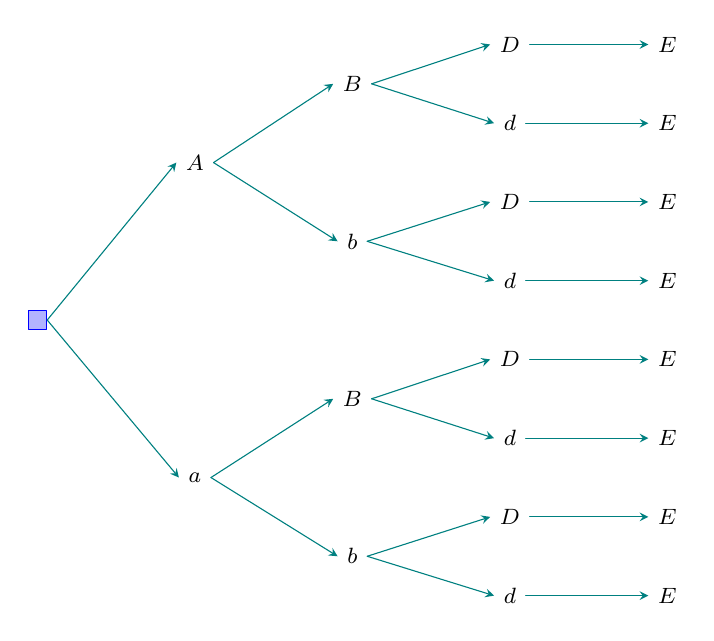
\begin{tikzpicture}[font=\footnotesize, line join=round, line cap=round, >=stealth,scale=1]
					\path(0,0)node[draw=blue,fill=blue!30](a){$ $ }
					++(2,2)node(b){$ A $}
					(a)++(2,-2)node(c){$ a $}
					;
					\path
					(b)++(2,1)node(b1){$ B $}
					(b)++(2,-1)node(b2){$ b $};
					\path (c)++(2,1)node(c1){$ B $}
					(c)++(2,-1)node(c2){$ b $}
					;
					
					\path
					(b1)++(2,0.5)node(b11){$ D $}
					(b1)++(2,-0.5)node(b12){$ d $};
					\path
					(b2)++(2,0.5)node(b21){$ D $}
					(b2)++(2,-0.5)node(b22){$ d $};
					
					\path (c1)++(2,0.5)node(c11){$ D $}
					(c1)++(2,-0.5)node(c12){$ d $}
					;
					\path (c2)++(2,0.5)node(c21){$ D $}
					(c2)++(2,-0.5)node(c22){$ d $}
					;
					\path (b11)++(2,0)node(e1) {$ E $}
					(b12)++(2,0)node(e2) {$ E $}
					(b21)++(2,0)node(e3) {$ E $}
					(b22)++(2,0)node(e4) {$ E $}
					(c11)++(2,0)node(e5) {$ E $}
					(c12)++(2,0)node(e6) {$ E $}
					(c21)++(2,0)node(e7) {$ E $}
					(c22)++(2,0)node(e8) {$ E $}
					;
					\draw[-stealth,teal,outer sep=0,inner sep=0](a.east)--(b.west);
					\draw[-stealth,teal,outer sep=0,inner sep=0](a.east)--(c.west);
					\draw[-stealth,teal,outer sep=0,inner sep=0](b.east)--(b1.west);
					\draw[-stealth,teal,outer sep=0,inner sep=0](b.east)--(b2.west);
					\draw[-stealth,teal,outer sep=0,inner sep=0](c.east)--(c1.west);
					\draw[-stealth,teal,outer sep=0,inner sep=0](c.east)--(c2.west);
					\draw[-stealth,teal,outer sep=0,inner sep=0](b1.east)--(b11.west);
					\draw[-stealth,teal,outer sep=0,inner sep=0](b1.east)--(b12.west);
					\draw[-stealth,teal,outer sep=0,inner sep=0](c1.east)--(c11.west);
					\draw[-stealth,teal,outer sep=0,inner sep=0](c1.east)--(c12.west);
					\draw[-stealth,teal,outer sep=0,inner sep=0](b2.east)--(b21.west);
					\draw[-stealth,teal,outer sep=0,inner sep=0](b2.east)--(b22.west);
					\draw[-stealth,teal,outer sep=0,inner sep=0](c2.east)--(c21.west);
					\draw[-stealth,teal,outer sep=0,inner sep=0](c2.east)--(c22.west);
					\draw[-stealth,teal,outer sep=0,inner sep=0](b11.east)--(e1.west);
					\draw[-stealth,teal,outer sep=0,inner sep=0](b12.east)--(e2.west);
					\draw[-stealth,teal,outer sep=0,inner sep=0](b21.east)--(e3.west);
					\draw[-stealth,teal,outer sep=0,inner sep=0](b22.east)--(e4.west);
					\draw[-stealth,teal,outer sep=0,inner sep=0](c11.east)--(e5.west);
					\draw[-stealth,teal,outer sep=0,inner sep=0](c12.east)--(e6.west);
					\draw[-stealth,teal,outer sep=0,inner sep=0](c21.east)--(e7.west);
					\draw[-stealth,teal,outer sep=0,inner sep=0](c22.east)--(e8.west);
				\end{tikzpicture}
			\end{center}
			\item Từ sơ đồ hình cây, ta có $ 8 $ loại giao tử kiểu gen $ AaBbDdEE $.
	\end{enumerate}}
\end{vd}

% #3846 | Archive/SP_KhoLatex/ID6_old/5D1.tex | mã gốc 1D2Y1-2
\begin{bt}%[Tex hóa SGK CD-CT,T7/22, TVN-001]%[1D2Y1-2]
	Từ các chữ số $ 1 $, $ 2 $, $ 3 $, $ 4 $, $ 5 $, $ 6 $ ta lập ra số tự nhiên gồm ba chữ số, chia hết cho $ 5 $. Có thể lập được bao nhiêu số như thế?
	\loigiai{Gọi số cần tìm có dạng: $ \overline{abc} $ với $ a $, $ b $, $ c \in X=\{1;2;3;4;5;6\}$.\\
		Việc lập số $ \overline{abc} $ là thực hiện ba hành động liên tiếp: chọn $ c $, chọn $ b $ và chọn $ a $. Các chữ số $ a $, $ b $ và $ c $ có thể giống nhau.\\
		Chọn $ c =5$ có $ 1 $ cách chọn.\\
		Chọn $ a\in X$ có $ 6 $ cách chọn.\\
		Chọn $ b\in X$ có $ 6 $ cách chọn.\\
		Theo quy tắc nhân, có $ 1\cdot 6\cdot 6=36 $ (số).
		
	}
\end{bt}

% #3847 | Archive/SP_KhoLatex/ID6_old/5D1.tex | mã gốc 1D2Y1-2
\begin{bt}%[Tex hóa SGK CD-CT,T7/22, TVN-001]%[1D2Y1-2]
	Từ các chữ số $1$, $2$, $3$, $4$, $5$, $6$, $7$, lập được bao nhiêu?
	\begin{enumerate}
		\item  Số chẵn gồm ba chữ số?
		\item  Số chẵn gồm ba chữ số đôi một khác nhau?
	\end{enumerate}
	\loigiai{Gọi số cần tìm có dạng: $ \overline{abc} $ với $ a $, $ b $, $ c \in X=\{1;2;3;4;5;6;7\}$.\\
		\begin{enumerate}
			\item  	Việc lập số $ \overline{abc} $ là thực hiện ba hành động liên tiếp: chọn $ c $, chọn $ b $ và chọn $ a $. Các chữ số $ a $, $ b $ và $ c $ có thể giống nhau.\\
			Chọn $ c\in \{2;4;6\}$ có $ 3 $ cách chọn.\\
			Chọn $ a\in X$ có $ 7 $ cách chọn.\\
			Chọn $ b\in X$ có $ 7 $ cách chọn.\\
			Theo quy tắc nhân, có $ 3\cdot 7\cdot 7=147 $ (số).
			\item  	Việc lập số $ \overline{abc} $ là thực hiện ba hành động liên tiếp: chọn $ c $, chọn $ b $ và chọn $ a $. Các chữ số $ a $, $ b $ và $ c $ đôi một khác nhau.\\
			Chọn $ c\in \{2;4;6\}$ có $ 3 $ cách chọn.\\
			Chọn $ a\in X\setminus\{c\}$ có $ 6 $ cách chọn.\\
			Chọn $ b\in X\setminus \{c;a\}$ có $ 5 $ cách chọn.\\
			Theo quy tắc nhân, có $ 3\cdot 6\cdot 5=90 $ (số).
		\end{enumerate}
		
	}
\end{bt}

% #3848 | Archive/SP_KhoLatex/ID6_old/5D1.tex | mã gốc 1D2Y1-1
\begin{bt}%[Tex hóa SGK CD-CT,T7/22, TVN-001]%[1D2Y1-1]
	Trong một trường trung học phổ thông, khối $ 10 $ có $ 245 $ học sinh nam và $ 235 $ học sinh nữ.
	\begin{enumEX}{1}
		\item Nhà trường cần chọn một học sinh ở khối $ 10 $ đi dự buổi giao lưu với học sinh các trường trung học phổ thông trong tỉnh. Hỏi nhà trường có bao nhiêu cách chọn?
		\item Nhà trường cần chọn hai học sinh ở khối $ 10 $ trong đó có $ 1 $ nam và $ 1 $ nữ đi dự trại hè của học sinh trong tỉnh. Hỏi nhà trường có bao nhiêu cách chọn?
	\end{enumEX}
	\loigiai{
		\begin{enumEX}{1}
			\item Tổng số học sinh khối $ 10 $ là $ 245+235=470 $ học sinh. Có $ 470 $ cách chọn $ 1 $ học sinh đi dự buổi giao lưu trong tỉnh.
			\item Chọn $ 1 $ học sinh nam có $ 245 $ cách, chọn $ 1 $ học sinh nữ có $ 235 $ cách. Theo quy tắc nhân có $ 245\cdot 235=57~575 $ cách chọn $ 1 $ học sinh nam và $ 1 $ học sinh nữ.
		\end{enumEX}
		
		
	}
\end{bt}

% #3849 | Archive/SP_KhoLatex/ID6_old/5D1.tex | mã gốc 1D2Y1-1
\begin{bt}%[Tex hóa SGK CD-CT,T7/22, TVN-001]%[1D2Y1-1]
	Trong giải thi đấu bóng đá World Cup, vòng bảng có $ 32 $ đội tham gia, được chia làm $ 8 $ bảng, mỗi bảng có $ 4 $ đội đấu vòng tròn một lượt. Tính số trận đấu được thi đấu trong vòng bảng theo thể thức trên.
	\loigiai{
		Giả sử trong một bảng có $ 4 $ đội là $ A $, $ B $, $ C $ và $ D $. Khi đó:\\
		Đội $ A $ gặp các đội $ B $, $ C $ và $ D $: Có $ 3 $ trận.\\
		Đội $ B $ gặp các đội $ C $, $ D $: Có $ 2 $ trận.\\
		Đội $ C $ gặp đội $ D $: Có $ 1 $ trận.\\
		Tổng số trận mỗi bảng là $ 3+2+1=6 $ trận.\\ Vậy có tất cả $ 6\cdot 8=48 $ trận ở tất cả các bảng đấu. 
		
	}
\end{bt}

% #3850 | Archive/SP_KhoLatex/ID6_old/5D1.tex | mã gốc 1D2Y1-2
\begin{bt}%[Tex hóa SGK CD-CT,T7/22, TVN-001]%[1D2Y1-2]
	Ở Canada, mã bưu chính có $ 6 $ kí tự gồm: $ 3 $ chữ cái in hoa (trong số $ 26 $ chữ cái tiếng Anh) và $ 3 $ chữ số. Mỗi mã bưu chính bắt đầu bằng $ 1 $ chữ cái và xen kẽ bằng $ 1 $ chữ số.
	\begin{flushright}
		\textit{(Nguồn: https://capath.vn/postal-code-canada)}
	\end{flushright}
	\begin{enumEX}{1}
		\item Có thể tạo được bao nhiêu mã bưu chính?
		\item Có thể tạo được bao nhiêu mã bắt đầu bằng chữ $S$ ?
		\item  Có thể tạo được bao nhiêu mã bắt đầu bằng chữ $S$ và kết thúc bằng chữ số $ 8 $ ?
	\end{enumEX}
	\loigiai{
		\begin{enumerate}
			\item 
			\begin{itemize}
				\item  Số cách chọn kí tự đầu tiên từ bảng chữ cái là: $ 26 $ (cách).
				\item  Số cách chọn kí tự thứ hai từ $ 10  $ chữ số là: $ 10 $ (cách).
				\item  Số cách chọn kí tự thứ ba từ bảng chữ cái là : $ 26 $ (cách).
				\item  Số cách chọn kí tự thứ tư từ $ 10  $ chữ số là: $ 10 $ (cách).
				\item  Số cách chọn kí tự thứ năm từ bảng chữ cái là : $ 26 $ (cách).
				\item Số cách chọn kí tự thứ sáu từ $ 10  $ chữ số là: $ 10 $ (cách).
			\end{itemize}
			Theo quy tắc nhân, có $26\cdot 10\cdot 26\cdot 10\cdot 26\cdot 10=17~576~000$ (cách).
			\item 
			\begin{itemize}
				\item  Do kí tự đầu tiên là S nên số cách chọn kí tự đầu tiên từ bảng chữ cái là: $ 1 $ (cách).\\
				\item Số cách chọn kí tự thứ hai từ $ 10  $ chữ số là: $ 10 $ (cách).
				\item Số cách chọn kí tự thứ ba từ bảng chữ cái là : $ 26 $ (cách).
				\item Số cách chọn kí tự thứ tư từ $ 10  $ chữ số là: $ 10 $ (cách).
				\item Số cách chọn kí tự thứ năm từ bảng chữ cái là : $ 26 $ (cách).
				\item Số cách chọn kí tự thứ sáu từ $ 10  $ chữ số là: $ 10 $ (cách).
			\end{itemize}
			Theo quy tắc nhân, có $1\cdot 10\cdot 26\cdot 10\cdot 26\cdot 10=676~000$ (cách).
			\item 
			\begin{itemize}
				\item  Do kí tự đầu tiên là S nên số cách chọn kí tự đầu tiên từ bảng chữ cái là: $ 1 $ (cách).
				\item  Số cách chọn kí tự thứ hai từ $ 10  $ chữ số là: $ 10 $ (cách).
				\item  Số cách chọn kí tự thứ ba từ bảng chữ cái là : $ 26 $ (cách).
				\item  Số cách chọn kí tự thứ tư từ $ 10  $ chữ số là: $ 10 $ (cách).
				\item  Số cách chọn kí tự thứ năm từ bảng chữ cái là : $ 26 $ (cách).
				\item  Do kí tự cuối là \lq\lq 8 \rq\rq \, nên số cách chọn kí tự thứ sáu từ bảng chữ cái là: $ 1 $ (cách).
			\end{itemize}
			Theo quy tắc nhân, có $1\cdot 10\cdot 26\cdot 10\cdot 26\cdot 1=67~600$ (cách).
		\end{enumerate}
	}
\end{bt}

% #3851 | Archive/SP_KhoLatex/ID6_old/5D1.tex | mã gốc 1D2Y1-2
\begin{bt}%[Tex hóa SGK CD-CT,T7/22, TVN-001]%[1D2Y1-2]
	Một hãng thời trang đưa ra một mẫu áo sơ mi mới có ba màu: trắng, xanh, đen. Mỗi loại có các cỡ $ S $, $ M $, $ L $, $ XL $, $ XXL $.
	\begin{enumerate}
		\item Vẽ sơ đồ hình cây biểu thị các loại áo sơ mi với màu và cỡ áo nói trên.
		\item Nếu một cửa hàng muốn mua tất cả các loại áo sơ mi (đủ loại màu và đủ loại cỡ áo) và mỗi loại một chiếc để về giới thiệu thì cần mua tất cả bao nhiêu chiếc áo sơ mi.
	\end{enumerate}
	
	\loigiai{
		\begin{enumerate}
			\item Sơ đồ hình cây biểu thị các loại áo sơ mi với màu và cỡ áo như sau:
			\begin{center}
				\begin{tikzpicture}[font=\footnotesize, line join=round, line cap=round, >=stealth,scale=1,rotate=-90]
					\path(0,0)node[draw=blue,fill=blue!30](a){Màu - Cỡ áo }
					++(2,5)node(b){Trắng}
					(a)++(2,0)node(c){Xanh}
					(a)++(2,-5)node(d){Đen}
					;
					\path
					(b)++(2,2)node(b1){$ S $}
					(b)++(2,1)node(b2){$M $}
					(b)++(2,0)node(b3){$L $}
					(b)++(2,-1)node(b4){$XL $}
					(b)++(2,-2)node(b5){$XXL $}	;
					\path
					(c)++(2,2)node(c1){$ S $}
					(c)++(2,1)node(c2){$M $}
					(c)++(2,0)node(c3){$L $}
					(c)++(2,-1)node(c4){$XL $}
					(c)++(2,-2)node(c5){$XXL $};
					\path
					(d)++(2,2)node(d1){$ S $}
					(d)++(2,1)node(d2){$M $}
					(d)++(2,0)node(d3){$L $}
					(d)++(2,-1)node(d4){$XL $}
					(d)++(2,-2)node(d5){$XXL $}	;
					\draw[-stealth,teal,outer sep=0,inner sep=0](a.south)--(b.north);
					\draw[-stealth,teal,outer sep=0,inner sep=0](a.south)--(c.north);
					\draw[-stealth,teal,outer sep=0,inner sep=0](a.south)--(d.north);
					
					\draw[-stealth,teal,outer sep=0,inner sep=0](b.south)--(b1.north);
					\draw[-stealth,teal,outer sep=0,inner sep=0](b.south)--(b2.north);
					\draw[-stealth,teal,outer sep=0,inner sep=0](b.south)--(b3.north);
					\draw[-stealth,teal,outer sep=0,inner sep=0](b.south)--(b4.north);
					\draw[-stealth,teal,outer sep=0,inner sep=0](b.south)--(b5.north);
					
					\draw[-stealth,teal,outer sep=0,inner sep=0](c.south)--(c1.north);
					\draw[-stealth,teal,outer sep=0,inner sep=0](c.south)--(c2.north);
					\draw[-stealth,teal,outer sep=0,inner sep=0](c.south)--(c3.north);
					\draw[-stealth,teal,outer sep=0,inner sep=0](c.south)--(c4.north);
					\draw[-stealth,teal,outer sep=0,inner sep=0](c.south)--(c5.north);	
					
					\draw[-stealth,teal,outer sep=0,inner sep=0](d.south)--(d1.north);
					\draw[-stealth,teal,outer sep=0,inner sep=0](d.south)--(d2.north);
					\draw[-stealth,teal,outer sep=0,inner sep=0](d.south)--(d3.north);
					\draw[-stealth,teal,outer sep=0,inner sep=0](d.south)--(d4.north);
					\draw[-stealth,teal,outer sep=0,inner sep=0](d.south)--(d5.north);					
				\end{tikzpicture}
			\end{center}
			\item Cần mua tất cả là $  3\cdot 5 =15 $ chiếc áo sơ mi.
		\end{enumerate}
		
	}
	
\end{bt}

% #3852 | Archive/SP_KhoLatex/ID6_old/5D1.tex | mã gốc 1D2Y1-2
\begin{bt}%[Tex hóa SGK CD-CT,T7/22, TVN-001]%[1D2Y1-2]
	Một khách sạn nhỏ chuẩn bị bữa ăn sáng gồm $ 2 $ đồ uống là: trà và cà phê; $ 3 $ món ăn là: phở, bún và cháo; $ 2 $ món tráng miệng là: bánh ngọt và sữa chua.
	\begin{enumerate}
		\item Vẽ sơ đồ hình cây biểu thị các cách chọn khẩu phần ăn gồm đủ ba loại: đồ uống, món ăn và món tráng miệng.
		\item Tính cách chọn khẩu phần ăn gồm: $ 1 $ đồ uống, $ 1 $ món ăn và $ 1 $ món tráng miệng.
	\end{enumerate}
	
	\loigiai{
		\begin{enumerate}
			\item Sơ đồ hình cây biểu thị các cách chọn khẩu phần ăn gồm đủ ba loại: đồ uống, món ăn và món tráng miệng như sau:
			\begin{center}
				\begin{tikzpicture}[font=\footnotesize, line join=round, line cap=round, >=stealth,scale=1.8]
					\path(0,0)node(a)[rectangle,draw=brown,text width=4cm,rounded corners=2mm,align=center]{Đồ uống - Món ăn - Tráng Miệng}
					++(-2.4,-1)node[rectangle,draw=brown,text width=1cm,rounded corners=2mm,align=center](b){Trà}
					(a)++(2.4,-1)node[rectangle,draw=brown,text width=2cm,rounded corners=2mm,align=center](c){Cà phê}
					;
					\path
					(b)++(-1.6,-1)node[rectangle,draw=brown,text width=1cm,rounded corners=2mm,align=center](b1){Phở}
					(b)++(0,-1)node[rectangle,draw=brown,text width=1cm,rounded corners=2mm,align=center](b2){Bún}
					(b)++(1.6,-1)node[rectangle,draw=brown,text width=1cm,rounded corners=2mm,align=center](b3){Cháo}
					;
					\path
					(b1)++(-0.4,-1)node[rectangle,draw=brown,text width=1cm,rounded corners=2mm,align=center](b11){Bánh ngọt}
					(b1)++(0.4,-1)node[rectangle,draw=brown,text width=1cm,rounded corners=2mm,align=center](b12){Sữa chua}
					;
					\path
					(b2)++(-0.4,-1)node[rectangle,draw=brown,text width=1cm,rounded corners=2mm,align=center](b21){Bánh ngọt}
					(b2)++(0.4,-1)node[rectangle,draw=brown,text width=1cm,rounded corners=2mm,align=center](b22){Sữa chua}
					;
					\path
					(b3)++(-0.4,-1)node[rectangle,draw=brown,text width=1cm,rounded corners=2mm,align=center](b31){Bánh ngọt}
					(b3)++(0.4,-1)node[rectangle,draw=brown,text width=1cm,rounded corners=2mm,align=center](b32){Sữa chua}
					;
					\path
					(c)++(-1.6,-1)node[rectangle,draw=brown,text width=1cm,rounded corners=2mm,align=center](c1){Phở}
					(c)++(0,-1)node[rectangle,draw=brown,text width=1cm,rounded corners=2mm,align=center](c2){Bún}
					(c)++(1.6,-1)node[rectangle,draw=brown,text width=1cm,rounded corners=2mm,align=center](c3){Cháo}
					;
					
					\path
					(c1)++(-0.4,-1)node[rectangle,draw=brown,text width=1cm,rounded corners=2mm,align=center](c11){Bánh ngọt}
					(c1)++(0.4,-1)node[rectangle,draw=brown,text width=1cm,rounded corners=2mm,align=center](c12){Sữa chua}
					;
					\path
					(c2)++(-0.4,-1)node[rectangle,draw=brown,text width=1cm,rounded corners=2mm,align=center](c21){Bánh ngọt}
					(c2)++(0.4,-1)node[rectangle,draw=brown,text width=1cm,rounded corners=2mm,align=center](c22){Sữa chua}
					;
					\path
					(c3)++(-0.4,-1)node[rectangle,draw=brown,text width=1cm,rounded corners=2mm,align=center](c31){Bánh ngọt}
					(c3)++(0.4,-1)node[rectangle,draw=brown,text width=1cm,rounded corners=2mm,align=center](c32){Sữa chua}
					;
					
					\draw[-stealth,teal,outer sep=0,inner sep=0](a.south)--++(-90:0.2)-|(b.north);
					\draw[-stealth,teal,outer sep=0,inner sep=0](a.south)--++(-90:0.2)-|(c.north);
					\draw[-stealth,teal,outer sep=0,inner sep=0](b.south)--++(-90:0.1)-|(b1.north);
					\draw[-stealth,teal,outer sep=0,inner sep=0](b.south)--++(-90:0.1)-|(b2.north);
					\draw[-stealth,teal,outer sep=0,inner sep=0](b.south)--++(-90:0.1)-|(b3.north);
					\draw[-stealth,teal,outer sep=0,inner sep=0](c.south)--++(-90:0.1)-|(c1.north);
					\draw[-stealth,teal,outer sep=0,inner sep=0](c.south)--++(-90:0.1)-|(c2.north);
					\draw[-stealth,teal,outer sep=0,inner sep=0](c.south)--++(-90:0.1)-|(c3.north);
					
					\draw[-stealth,teal,outer sep=0,inner sep=0](b1.south)--++(-90:0.1)-|(b11.north);
					\draw[-stealth,teal,outer sep=0,inner sep=0](b1.south)--++(-90:0.1)-|(b12.north);
					\draw[-stealth,teal,outer sep=0,inner sep=0](b2.south)--++(-90:0.1)-|(b21.north);
					\draw[-stealth,teal,outer sep=0,inner sep=0](b2.south)--++(-90:0.1)-|(b22.north);
					\draw[-stealth,teal,outer sep=0,inner sep=0](b3.south)--++(-90:0.1)-|(b31.north);
					\draw[-stealth,teal,outer sep=0,inner sep=0](b3.south)--++(-90:0.1)-|(b32.north);
					
					\draw[-stealth,teal,outer sep=0,inner sep=0](c1.south)--++(-90:0.1)-|(c11.north);
					\draw[-stealth,teal,outer sep=0,inner sep=0](c1.south)--++(-90:0.1)-|(c12.north);
					\draw[-stealth,teal,outer sep=0,inner sep=0](c2.south)--++(-90:0.1)-|(c21.north);
					\draw[-stealth,teal,outer sep=0,inner sep=0](c2.south)--++(-90:0.1)-|(c22.north);
					\draw[-stealth,teal,outer sep=0,inner sep=0](c3.south)--++(-90:0.1)-|(c31.north);
					\draw[-stealth,teal,outer sep=0,inner sep=0](c3.south)--++(-90:0.1)-|(c32.north);
				\end{tikzpicture}
			\end{center}
			\item Số cách chọn khẩu phần ăn gồm: $ 1 $ đồ uống, $ 1 $ món ăn và $ 1 $ món tráng miệng là $$ 2\cdot 3\cdot 2=12 \quad \text{ (cách)}.$$
		\end{enumerate}
		
	}
	
\end{bt}

% #3853 | Archive/SP_KhoLatex/ID6_old/5D1.tex | mã gốc 1D2Y1-2
\begin{bt}%[Tex hóa SGK CD-CT,T7/22, TVN-001]%[1D2Y1-2]
	Cho kiểu gen $ AaBbDdEe $. Giả sử quá trình giảm phân tạo ra giao tử bình thường, không xảy ra đột biến.
	\begin{enumerate}
		\item Vẽ sơ đồ hình cây biểu thị sự hình thành giao tử.
		\item Từ đó, tính số loại giao tử của kiểu gen $ AaBbDdEe $.
	\end{enumerate}
	
	\loigiai{
		\begin{enumerate}
			\item Sơ đồ hình cây biểu thị sự hình thành giao từ như sau:
			\begin{center}
				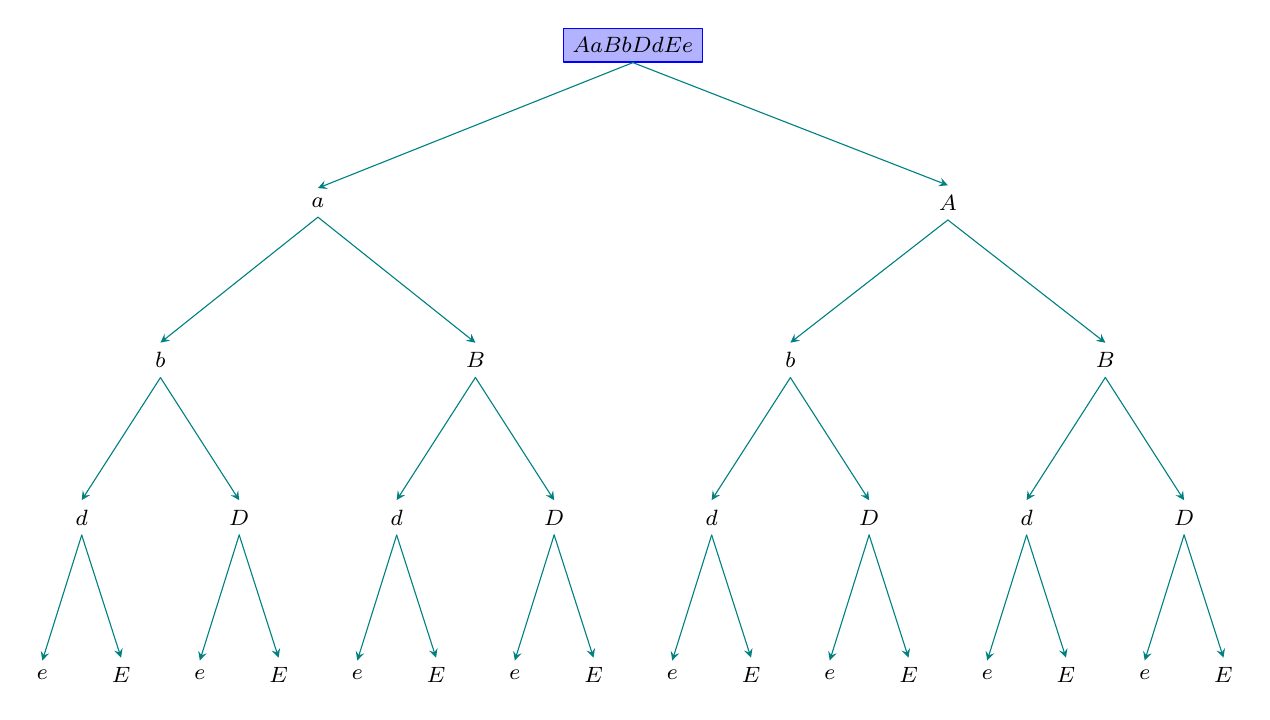
\begin{tikzpicture}[font=\footnotesize, line join=round, line cap=round, >=stealth,scale=1,rotate=-90]
					\path(0,0)node[draw=blue,fill=blue!30](a){$AaBbDdEe  $ }
					++(2,4)node(b){$ A $}
					(a)++(2,-4)node(c){$ a $}
					;
					\path
					(b)++(2,2)node(b1){$ B $}
					(b)++(2,-2)node(b2){$ b $};
					\path (c)++(2,2)node(c1){$ B $}
					(c)++(2,-2)node(c2){$ b $}
					;
					
					\path
					(b1)++(2,1)node(b11){$ D $}
					(b1)++(2,-1)node(b12){$ d $};
					\path
					(b2)++(2,1)node(b21){$ D $}
					(b2)++(2,-1)node(b22){$ d $};
					
					\path (c1)++(2,1)node(c11){$ D $}
					(c1)++(2,-1)node(c12){$ d $}
					;
					\path (c2)++(2,1)node(c21){$ D $}
					(c2)++(2,-1)node(c22){$ d $}
					;
					\path (b11)++(2,0.5)node(e1) {$ E $}
					(b11)++(2,-0.5)node(e2) {$ e $}	
					(b12)++(2,0.5)node(e3) {$ E $}
					(b12)++(2,-0.5)node(e4) {$ e $}	
					(b21)++(2,0.5)node(e5) {$ E $}
					(b21)++(2,-0.5)node(e6) {$ e $}		
					(b22)++(2,0.5)node(e7) {$ E $}
					(b22)++(2,-0.5)node(e8) {$ e $}	
					(c11)++(2,0.5)node(e9) {$ E $}
					(c11)++(2,-0.5)node(e10) {$ e $}	
					(c12)++(2,0.5)node(e11) {$ E $}
					(c12)++(2,-0.5)node(e12) {$ e $}	
					(c21)++(2,0.5)node(e13) {$ E $}
					(c21)++(2,-0.5)node(e14) {$ e $}		
					(c22)++(2,0.5)node(e15) {$ E $}
					(c22)++(2,-0.5)node(e16) {$ e $}			
					;
					\draw[-stealth,teal,outer sep=0,inner sep=0](a.south)--(b.north);
					\draw[-stealth,teal,outer sep=0,inner sep=0](a.south)--(c.north);
					\draw[-stealth,teal,outer sep=0,inner sep=0](b.south)--(b1.north);
					\draw[-stealth,teal,outer sep=0,inner sep=0](b.south)--(b2.north);
					\draw[-stealth,teal,outer sep=0,inner sep=0](c.south)--(c1.north);
					\draw[-stealth,teal,outer sep=0,inner sep=0](c.south)--(c2.north);
					\draw[-stealth,teal,outer sep=0,inner sep=0](b1.south)--(b11.north);
					\draw[-stealth,teal,outer sep=0,inner sep=0](b1.south)--(b12.north);
					\draw[-stealth,teal,outer sep=0,inner sep=0](c1.south)--(c11.north);
					\draw[-stealth,teal,outer sep=0,inner sep=0](c1.south)--(c12.north);
					\draw[-stealth,teal,outer sep=0,inner sep=0](b2.south)--(b21.north);
					\draw[-stealth,teal,outer sep=0,inner sep=0](b2.south)--(b22.north);
					\draw[-stealth,teal,outer sep=0,inner sep=0](c2.south)--(c21.north);
					\draw[-stealth,teal,outer sep=0,inner sep=0](c2.south)--(c22.north);
					\draw[-stealth,teal,outer sep=0,inner sep=0](b11.south)--(e1.north);
					\draw[-stealth,teal,outer sep=0,inner sep=0](b11.south)--(e2.north);
					\draw[-stealth,teal,outer sep=0,inner sep=0](b12.south)--(e3.north);
					\draw[-stealth,teal,outer sep=0,inner sep=0](b12.south)--(e4.north);
					\draw[-stealth,teal,outer sep=0,inner sep=0](b21.south)--(e5.north);
					\draw[-stealth,teal,outer sep=0,inner sep=0](b21.south)--(e6.north);
					\draw[-stealth,teal,outer sep=0,inner sep=0](b22.south)--(e7.north);
					\draw[-stealth,teal,outer sep=0,inner sep=0](b22.south)--(e8.north);
					\draw[-stealth,teal,outer sep=0,inner sep=0](c11.south)--(e9.north);
					\draw[-stealth,teal,outer sep=0,inner sep=0](c11.south)--(e10.north);
					\draw[-stealth,teal,outer sep=0,inner sep=0](c12.south)--(e11.north);
					\draw[-stealth,teal,outer sep=0,inner sep=0](c12.south)--(e12.north);
					\draw[-stealth,teal,outer sep=0,inner sep=0](c21.south)--(e13.north);
					\draw[-stealth,teal,outer sep=0,inner sep=0](c21.south)--(e14.north);
					\draw[-stealth,teal,outer sep=0,inner sep=0](c22.south)--(e15.north);
					\draw[-stealth,teal,outer sep=0,inner sep=0](c22.south)--(e16.north);
				\end{tikzpicture}
			\end{center}
			\item Số loại giao tử của kiểu gen $ AaBbDdEe $ là $ 16 $.
		\end{enumerate}
		
	}
	
\end{bt}

% #3854 | Archive/SP_KhoLatex/ID6_old/26-BienCoVaDinhNghiaCoDienCuaXacSuat.tex | mã gốc 1D2B4-1
\begin{ex}%[1D2B4-1]
	Một hộp chứa $ 12 $ tấm thẻ được đánh số  $ 1 $; $ 2 $; $ 3 $; $ 4 $; $ 5 $; $ 6 $; $ 7 $; $ 8 $; $ 9 $; $ 10 $; $ 11 $; $ 12 $. Rút ngẫu nhiên từ hộp đó một tấm thẻ.
	\begin{enumerate}
		\item Mô tả không gian mẫu $ \Omega $. Các kết quả có thể có đồng khả năng không?
		\item Xét biến cố $ \mathrm{E} $: \lq\lq Rút được thẻ ghi số nguyên tố\rq\rq. Biến cố $ \mathrm{E} $ là tập con   nào của không gian mẫu?
		\item Phép thử có bao nhiêu kết quả có thể? Biến cố $ \mathrm{E} $ có bao nhiêu kết quả thuận lợi? Từ đó, hãy tính xác suất của biến cố  $ \mathrm{E} $.
	\end{enumerate}
	\loigiai{
		\begin{enumerate}
			\item $ \Omega=\{1; 2;\ldots ; 12\} $. Vì rút ngẫu nhiên nên các kết quả có thể là đồng khả năng.
			\item $ \mathrm{E}=\{2; 3; 5; 7; 11\} $.
			\item Phép thử có $ 12 $ kết quả có thể. Biến cố $ \mathrm{E} $ có $ 5 $ kết quả thuận lợi. Từ đó, $ \mathrm{P}(\mathrm{E})=\dfrac{n(\mathrm{E})}{n(\Omega)}=\dfrac{5}{12} $.
		\end{enumerate}
	}
\end{ex}

% #3855 | Archive/SP_KhoLatex/ID6_old/26-BienCoVaDinhNghiaCoDienCuaXacSuat.tex | mã gốc 1D2B4-1
\begin{ex}%[1D2B4-1]
	Hộp thứ nhất đựng $4$ tấm thẻ  cùng loại được đánh số từ $1$ đến $4$. Hộp thứ hai đựng $6$ tấm thẻ cùng loại được đánh số từ $1$ đến $6$. Lấy ra ngẫu nhiên từ mỗi hộp một tấm thẻ.
	\begin{enumerate}
		\item Hãy xác định không gian mẫu của phép thử.
		\item Gọi $A$ là biến cố \lq\lq Hai thẻ lấy ra có cùng số\rq\rq. Hãy liệt kê các kết quả thuận lợi cho $A$ và tính xác suất của biến cố $A$.
		\item Gọi $B$ là biến cố \lq\lq Tổng hai số trên hai thẻ lấy ra lớn hơn 8\rq\rq. Hãy liệt kê các kết quả thuận lợi cho $B$ và tính xác suất của biến cố $B$.
	\end{enumerate}
	\loigiai{
		\begin{enumerate}
			\item Kết quả của mỗi lần thử là một cặp $(i;j)$ với $i\in\{1;2;3;4\}$ là số trên thẻ được lấy ra từ hộp thứ nhất và $j\in\{1;2;3;4;5;6\}$ là số thẻ được lấy ra từ hộp thứ hai. Không gian mẫu của phép thử là
			\begin{align*}
			\Omega=\{&(1;1);(1;2);(1;3);(1;4);(1;5);(1;6);\\
			&(2;1);(2;2);(2;3);(2;4);(2;5);(2;6);\\
			&(3;1);(3;2);(3;3);(3;4);(3;5);(3;6);\\
			&(4;1);(4;2);(4;3);(4;4);(4;5);(4;6)\}.
			\end{align*}
			\item Không gian mẫu gồm $24$ kết quả, tức là $n(\Omega)=24$.\\
			Biến cố $A=\{(1;1);(2;2);(3;3);(4;4)\}$.\\
			Số các kết quả thuận lợi cho $A$ là $n(A)=4$. Do đó, xác suất của biến cố $A$ là
			$$\mathrm P(A)=\dfrac{4}{24}=\dfrac{1}{6}.$$
			\item Biến cố $B=\{(3;6);(4;5);(4;6);\}$.\\
			Số các kết quả thuận lợi cho $B$ là $n(B)=3$. Do đó, xác suất của biến cố $B$ là $$\mathrm P(B)=\dfrac{3}{24}=\dfrac{1}{8}.$$
		\end{enumerate}
	}
\end{ex}

% #3856 | Archive/SP_KhoLatex/ID6_old/26-BienCoVaDinhNghiaCoDienCuaXacSuat.tex | mã gốc 1D2B4-1
\begin{ex}%[1D2B4-1]
	Gieo hai con xúc xắc cân đối và đồng chất. Tính xác suất của các biến cố 
	\begin{enumerate}
		\item \lq\lq Hai mặt xuất hiện có cùng số chấm \rq\rq;
		\item \lq\lq Tổng số chấm trên hai mặt bằng $9$\rq\rq.
	\end{enumerate}
	\loigiai{
		\begin{enumerate}
			\item Không gian mẫu là $\Omega=\{(i;j)\,|\,1\leq i,j\leq 6\}$. Do đó $n(\Omega)=6\cdot 6=36$.\\
			Biến cố $A=\{(1;1);(2;2);(3;3);(4;4);(5;5);(6;6)\}$.\\
			Số các kết quả thuận lợi cho $A$ là $n(A)=6$. Do đó, xác suất của biến cố $A$ là
			$$\mathrm P(A)=\dfrac{6}{36}=\dfrac{1}{6}.$$
			\item Biến cố $B=\{(6;3);(5;4);(4;5);(3;6)\}$.\\
			Số các kết quả thuận lợi cho $B$ là $n(B)=4$. Do đó, xác suất của biến cố $B$ là $$\mathrm P(B)=\dfrac{4}{36}=\dfrac{1}{9}.$$
		\end{enumerate}
	}
\end{ex}

% #3857 | Archive/SP_KhoLatex/ID6_old/26-BienCoVaDinhNghiaCoDienCuaXacSuat.tex | mã gốc 1D2B4-1
\begin{ex}%[1D2B4-1]
	Trong hộp có $5$ viên bi xanh và $7$ viên bi trắng có kích thước và khối lượng như nhau. Ta lấy hai viên bi bằng hai cách như sau:
	\begin{itemize}
		\item Cách thứ nhất: Lấy ngẫu nhiên một viên bi, xem màu rồi trả lại hộp. Sau đó lại lấy một viên bi một cách ngẫu nhiên.
		\item Cách thứ hai: Lấy cùng lúc hai viên bi từ hộp. 
	\end{itemize}
	Gọi $A$ là biến cố \lq\lq Cả hai bi lấy ra đều là màu trắng\rq\rq. Với cách lấy bi nào thì biến cố $A$ có khả năng xảy ra cao hơn.
	\loigiai{
		Theo cách lấy bi thứ nhất, áp dụng quy tắc nhân ta có số phần tử của không gian mẫu là $n(\Omega)=12\cdot 12=144$.\\
		Số khả năng thuận lợi cho $A$ là $7\cdot 7=49$.\\
		Do đó xác suất của biến cố $A$ theo cách lấy thứ nhất là $\dfrac{49}{144}$.\\
		Theo cách lấy bi thứ hai, số phần tử của không gian mẫu là $n(\Omega)=\mathrm C_{12}^2=66$.\\
		Số khả năng thuận lợi cho $A$ là $n(A)=\mathrm C_7^2=21$.\\
		Do đó xác suất của biến cố $A$ theo cách lấy thứ hai là $\dfrac{21}{66}=\dfrac{7}{22}$.\\
		Ta có $\dfrac{49}{144}>\dfrac{7}{22}$ nên với cách lấy bi thứ nhất thì biến cố $A$ có khả năng xảy ra cao hơn.
	}
\end{ex}

% #3858 | Archive/SP_KhoLatex/ID6_old/26-BienCoVaDinhNghiaCoDienCuaXacSuat.tex | mã gốc 1D2B4-1
\begin{ex}%[1D2B4-1]
	Lấy ra ngẫu nhiên đồng thời $2$ viên bi từ một hộp có chứa $5$ bi xanh và $5$ bi đỏ có cùng kích thước và trọng lượng. Biến cố lấy được $2$ viên bi cùng màu hay $2$ viên bi khác màu có khả năng xảy ra cao hơn?
	\loigiai{
		Số phần tử của không gian mẫu là $n(\Omega)=\mathrm C_{10}^2=45$.\\
		Gọi $A$ là biến cố lấy được $2$ viên bi cùng màu, $B$ là biến cố lấy được $2$ viên bi khác màu.\\
		Ta có $n(A)=\mathrm C_5^2+\mathrm C_5^2=20$. Suy ra $\mathrm P(A)=\dfrac{20}{45}=\dfrac{4}{9}$.\\
		Ta có $n(B)=5\cdot 5=25$. Suy ra $\mathrm P(B)=\dfrac{25}{45}=\dfrac{5}{9}$.\\
		Vì $P(B)>P(A)$ nên biến cố lấy được hai bi khác màu có khả năng xảy ra cao hơn biến cố lấy được hai bi cùng màu.
	}
\end{ex}

% #3859 | Archive/SP_KhoLatex/ID6_old/26-BienCoVaDinhNghiaCoDienCuaXacSuat.tex | mã gốc 1D2B4-1
\begin{ex}%[1D2B4-1]
	Gieo một đồng xu cân đối liên tiếp ba lần. Gọi $ \mathrm{E} $ là biến cố: \lq\lq Có hai lần xuất hiện mặt sấp và một lần xuất hiện mặt ngửa\rq\rq. Tính xác suất của biến cố $ \mathrm{E} $.
	\loigiai{
		Kí hiệu $ \mathrm{S} $ và $ \mathrm{N} $ tương ứng là đồng xu ra mặt sấp và đồng xu ra mặt ngửa.\\
		Không gian mẫu $ \Omega=\{ \mathrm{S} \mathrm{S} \mathrm{N};  \mathrm{S} \mathrm{N} \mathrm{S};  \mathrm{S} \mathrm{N} \mathrm{N};  \mathrm{S} \mathrm{S} \mathrm{S};  \mathrm{N} \mathrm{S} \mathrm{N}; \mathrm{N} \mathrm{N} \mathrm{S};  \mathrm{N} \mathrm{N} \mathrm{N};  \mathrm{N} \mathrm{S} \mathrm{S}\} $.\\
		$\mathrm{E}=\{ \mathrm{S} \mathrm{S} \mathrm{N};  \mathrm{S} \mathrm{N} \mathrm{S};  \mathrm{N} \mathrm{S} \mathrm{S}$.\\
		Ta có $ n(\Omega)=8 $; $ n(\mathrm{E})=3 $. Do đồng xu cân đối nên các kết quả  có thể là đồng khả năng.\\
		Vậy $ \mathrm{P}(\mathrm{E})=\dfrac{n(\mathrm{E})}{n(\Omega)}=\dfrac{3}{8} $.
	}
\end{ex}

% #3860 | Archive/SP_KhoLatex/ID6_old/26-BienCoVaDinhNghiaCoDienCuaXacSuat.tex | mã gốc 1D2B5-2
\begin{ex}%[1D2B5-2]
	Gieo một con xúc xắc $4$ mặt cân đối và đồng chất ba lần. Tính xác suất của các biến cố:
	\begin{enumerate}
		\item \lq\lq Tổng các số xuất hiện ở đỉnh phía trên của con xúc xắc trong ba lần gieo lớn hơn $2$\rq\rq.
		\item \lq\lq Có đúng một lần số xuất hiện ở đỉnh phía trên của con xúc xắc là $2$\rq\rq.
	\end{enumerate}
	\loigiai
	{
		\begin{enumerate}
			\item Biến cố \lq\lq Tổng các số xuất hiện ở đỉnh phía trên của con xúc xắc trong ba lần gieo lớn hơn $2$\rq\rq\ là biến cố chắc chắn nên có xác suất bằng $1$.
			\item Không gian mẫu $\Omega= \{(a,b,c) \text{ với } 1\le a,b,c \le 4\}$, trong đó $a$, $b$, $c$ lần lượt là số chấm xuất hiện trong các lần gieo 1, lần gieo 2, lần gieo 3.\\
			Số các kết quả có thể xảy ra là $n(\Omega)= 4^3=64$.\\
			Gọi $B$ là biến cố \lq\lq Có đúng một lần số xuất hiện ở đỉnh phía trên của con xúc xắc là $2$\rq\rq.\\
			Số $2$ xuất hiện trong $1$ lần gieo, có $3$ cách.\\
			Hai lần gieo còn lại, số xuất hiện thuộc tập $\{1; 3; 4\}$, có $3^2$ cách.\\
			Theo quy tắc nhân, ta có $n(B)= 3\cdot 3^2=27$.\\
			Vậy xác suất cần tìm là $\mathrm{P}(B)= \dfrac{27}{64}$.
		\end{enumerate}
	}
\end{ex}

% #3861 | Archive/SP_KhoLatex/ID6_old/26-BienCoVaDinhNghiaCoDienCuaXacSuat.tex | mã gốc 1D2B5-2
\begin{ex}%[1D2B5-2]
	Gieo một xúc xắc hai lần liên tiếp. Tính xác suất của mỗi biến cố sau:
	\begin{enumerate}
		\item \lq\lq Tổng số chấm xuất hiện trong hai lần gieo không bé hơn $10$\rq\rq.
		\item \lq\lq Mặt $6$ chấm xuất hiện ít nhất một lần\rq\rq.
	\end{enumerate}
	\loigiai
	{
		Không gian mẫu $\Omega= \{(a, b), \, 1\le a, b\le 6\}$, trong đó $a$, $b$ tương ứng là số chấm xuất hiện ở lần gieo thứ nhất và thứ hai $\Rightarrow n(\Omega)= 6\cdot 6=36$.
		\begin{enumerate}
			\item Gọi $A$ là biến cố \lq\lq Tổng số chấm xuất hiện trong hai lần gieo không bé hơn $10$\lq\lq.\\
			Ta có $A=\{(4,6); (5,5), (5,6); (6,4); (6,5); (6,6)\}$. Do đó $n(A)= 6$.\\
			Vậy xác suất cần tìm là $\mathrm{P}(A)= \dfrac{6}{36}= \dfrac{1}{6}$.
			\item Gọi $B$ là biến cố \lq\lq Mặt $6$ chấm xuất hiện ít nhất một lần\lq\lq.\\
			Ta có $B=\{(6,1); (6,2); (6,3); (6,4); (6,5); (6,6); (1,6); (2,6); (3,6); (4,6); (5,6)\}$.\\
			Suy ra $n(B)=11$.\\
			Vậy xác suất cần tìm là $\mathrm{P}(B)= \dfrac{11}{36}$.
		\end{enumerate}
	}
\end{ex}

% #3862 | Archive/SP_KhoLatex/ID6_old/26-BienCoVaDinhNghiaCoDienCuaXacSuat.tex | mã gốc 1D2B5-2
\begin{ex}%[1D2B5-2]
	Gieo một đồng xu và một con xúc xắc đồng thời. Tính xác suất của biến cố $A$: \lq\lq Đồng xu xuất hiện mặt sấp hoặc con xúc xắc xuất hiện mặt $5$ chấm\rq\rq.
	\loigiai
	{
		Không gian mẫu $\Omega= \{(1,S); (2,S); (3,S); (4,S); (5,S); (6,S); (1,N); (2,N); (3,N); (4,N); (5,N); (6,N)\}$. Suy ra $n(\Omega)= 12$.\\
		Ta có $A=\{(1,S); (2,S); (3,S); (4,S); (5,S); (6,S); (5,N)\}$ $\Rightarrow n(A)=7$.\\
		Vậy xác suất cần tìm là $\mathrm{P}(A)= \dfrac{7}{12}$.
	}
\end{ex}

% #3863 | Archive/SP_KhoLatex/ID6_old/26-BienCoVaDinhNghiaCoDienCuaXacSuat.tex | mã gốc 1D2B5-2
\begin{ex}%[1D2B5-2]
	Có hai hộp $I$ và $II$. Hộp thứ nhất chứa $12$ tấm thẻ vàng đánh số từ $1$ đến $12$. Hộp thứ hai chứa $6$ tấm thẻ đỏ đánh số từ $1$ đến $6$. Rút ngẫu nhiên từ mỗi hộp một tấm thẻ. Tính xác suất của các biến cố.
	\begin{enumerate}
		\item $A$: \lq\lq Cả hai tấm thẻ đều mang số $5$\rq\rq.
		\item $B$: \lq\lq Tổng hai số trên hai tấm thẻ bằng $6$\rq\rq.
	\end{enumerate}
	\loigiai
	{
		Không gian mẫu $\Omega= \{(a,b) \text{ với } 1\le a\le 12 \text{ và } 1\le b\le 6\}$, trong đó $a$, $b$ lần lượt là số ghi trên các thẻ được rút ra từ hộp $I$ và hộp $II$.\\
		Ta có $n(\Omega)= 12\cdot 6=72$.
		\begin{enumerate}
			\item $A= \{(5,5)\} \Rightarrow n(A)=1$.\\
			Vậy xác suất cần tìm là $\mathrm{P}(A)= \dfrac{1}{72}$.
			\item $B= \{(1,5), (2,4), (3,3), (4,2), (5,1)\} \Rightarrow n(B)=5$.\\
			Vậy xác suất cần tìm là $\mathrm{P}(B)= \dfrac{5}{72}$.
		\end{enumerate}
	}
\end{ex}

% #3864 | Archive/SP_KhoLatex/ID6_old/26-BienCoVaDinhNghiaCoDienCuaXacSuat.tex | mã gốc 1D2B5-2
\begin{ex}%[1D2B5-2]
	Có ba chiếc hộp. Hộp thứ nhất chứa $5$ tấm thẻ đánh số từ $1$ đến $5$. Hộp thứ hai chứa $6$ tấm thẻ đánh số từ $1$ đến $6$. Hộp thứ ba chứa $7$ tấm thẻ đánh số từ $1$ đến $7$. Từ mỗi hộp rút ngẫu nhiên một tấm thẻ. Tính xác suất để tổng ba số ghi trên ba tấm thẻ bằng $15$.
	\loigiai
	{
		Không gian mẫu $\Omega= \{(a,b,c) \text{ với } 1\le a\le 5,\, 1 \le b\le 6,\, 1\le c\le 7\}$. Suy ra $n(\Omega)= 5\cdot 6\cdot 7 = 210$.\\
		Gọi $A$ là biến cố \lq\lq Tổng ba số ghi trên ba tấm thẻ bằng $15$\rq\rq.\\
		Ta có $A=\{(2,6,7); (3,6,6); (3,5,7); (4,6,5); (4,5,6); (4,4,7); (5,3,7); (5,4,6); (5,5,5); (5,6,4)\}$.\\
		Do đó $n(A)=10$.\\
		Vậy xác suất cần tìm là $\mathrm{P}(A)= \dfrac{10}{210}= \dfrac{1}{21}$.
	}
\end{ex}

% #3940 | Archive/SP_KhoLatex/SP_Đề Theo Bài-Khối 11/1-B30.tex | mã gốc 1D9H1-3
\begin{ex}%[1D9H1-3]%[Dự án 2025 - Đề cấu trúc mới của Bộ theo bài]
Gieo hai đồng xu $A$ và $B$ một cách độc lập. Đồng xu $A$ được chế tạo cân đối. Đồng xu $B$ được chế tạo không cân đối nên xác suất xuất hiện mặt sấp gấp $3$ lần xác suất xuất hiện mặt ngửa. Xét tính đúng sai của các mệnh đề sau.
\choiceTF
{\True Xác suất đồng xu $A$ xuất hiện mặt ngửa bằng $\dfrac{1}{2}$}
{\True Xác suất đồng xu $B$ xuất hiện mặt ngửa bằng $\dfrac{1}{4}$}
{Khi gieo hai đồng xu một lần thì xác suất cả hai đều ngửa bằng $\dfrac{1}{12}$}
{Khi gieo hai đồng xu hai lần thì xác suất cả hai đồng xu đều ngửa bằng $\dfrac{1}{32}$}
\loigiai
{
\begin{itemchoice}
\itemch Đúng. Vì gọi $X$ là biến cố: \lq\lq Đồng xu $A$ xuất hiện mặt ngửa\rq\rq.\\
Do đồng xu $A$ chế tạo cân đối nên $\mathrm{P}(X)=\dfrac{1}{2}$.
\itemch Đúng. Vì gọi $Y$ là biến cố: \lq\lq Đồng xu $B$ xuất hiện mặt ngửa\rq\rq.\\
Do đồng xu $B$ được chế tạo không cân đối nên xác suất xuất hiện mặt sấp gấp $3$ lần xác suất xuất hiện mặt ngửa, do đó $\mathrm{P}(Y)=\dfrac{1}{4}$.
\itemch Sai. Vì $X\cap Y$ là biến cố \lq\lq Hai đồng xu đều ngửa\rq\rq\ và $X$, $Y$ là hai biến cố độc lập nên $\mathrm{P}(XY)=\mathrm{P}(X)\cdot\mathrm{P}(Y)=\dfrac{1}{2}\cdot\dfrac{1}{4}=\dfrac{1}{8}$.
\itemch Sai. Vì xác suất để trong một lần gieo cả hai đồng xu đều ngửa là $\dfrac{1}{8}$.\\
Suy ra xác suất khi gieo hai lần thì cả hai lần đó hai đồng xu đều ngửa là $\dfrac{1}{8}\cdot\dfrac{1}{8}=\dfrac{1}{64}$.
\end{itemchoice}
}
\end{ex}

% #3943 | Archive/SP_KhoLatex/SP_Đề Theo Bài-Khối 11/1-B30.tex | mã gốc 1D9H1-3
\begin{ex}%[1D9H1-3]%[Dự án 2025 - Đề cấu trúc mới của Bộ theo bài]
Hộp $A$ đựng $5$ tấm thẻ được đánh số từ $1$ đến $5$, hộp $B$ đựng $6$ tấm thẻ được đánh số từ $1$ đến $6$, hai thẻ khác nhau ở mỗi hộp đánh hai số khác nhau. Chọn ngẫu nhiên từ hộp $A$ một tấm thẻ và từ hộp $B$ hai tấm thẻ. Gọi $X$ là biến cố: \lq\lq Chọn được thẻ mang số lẻ từ hộp $A$\rq\rq, $Y$ là biến cố: \lq\lq Chọn được thẻ mang số chẵn từ hộp $A$\rq\rq, và $Z$ là biến cố: \lq\lq Chọn được hai thẻ mang số lẻ từ hộp $B$\rq\rq. Tính xác suất để tích số được ghi trên ba tấm thẻ thu được là số chẵn.
\shortans{$0{,}88$}
\loigiai
{
Gọi $U$ là biến cố \lq\lq Tích ba số ghi trên ba thẻ là số lẻ\rq\rq.\\
Suy ra $\overline{U}$ là biến cố \lq\lq Tích ba số ghi trên ba thẻ thu được là số chẵn\rq\rq.\\
Để có được tích ba số ghi trên ba thẻ là số lẻ thì cả ba thẻ thu được đều mang số lẻ.\\
Suy ra $U=X\cap Z$. \\
Ta có $\mathrm{P}(X)=\dfrac{3}{5}$ và $\mathrm{P}(Z)=\dfrac{\mathrm{C}_{3}^{2}}{\mathrm{C}_{6}^{2}}=\dfrac{1}{5}$. \\
Vì $X$ và $Z$ là các biến cố độc lập nên $\mathrm{P}(X\cap Z)=\mathrm{P}(X)\cdot\mathrm{P}(Z)=\dfrac{3}{5}\cdot\dfrac{1}{5}=\dfrac{3}{25}$.\\
Vậy $\mathrm{P}\left(\overline{U}\right)=1-\mathrm{P}(U)=1-\dfrac{3}{25}=\dfrac{22}{25}=0{,}88$.
}
\end{ex}

% #3944 | Archive/SP_KhoLatex/SP_Đề Theo Bài-Khối 11/1-B30.tex | mã gốc 1D9H2-3
\begin{ex}%[1D9H2-3]%[Dự án 2025 - Đề cấu trúc mới của Bộ theo bài]
Một lô hàng có $20$ sản phẩm giống nhau trong đó có $4$ sản phẩm không đạt chất lượng còn lại là sản phẩm đạt chất lượng tốt. Mỗi lần kiểm tra, người ta chọn ra ngẫu nhiên $2$ sản phẩm. Tính xác suất để lấy ra được ít nhất một sản phẩm tốt \textit{(làm tròn đến hàng phần trăm)}.
\shortans{$0{,}97$}
\loigiai
{
Gọi $A$ là biến cố: \lq\lq Lấy ra một sản phẩm tốt và một sản phẩm không đạt chất lượng\rq\rq, \\
suy ra $\mathrm{P}(A)=\dfrac{\mathrm{C}_{16}^{1}\cdot\mathrm{C}_{4}^{1}}{\mathrm{C}_{20}^{2}}$.\\
Gọi $B$ là biến cố: \lq\lq Lấy ra hai sản phẩm đều tốt\rq\rq, suy ra $\mathrm{P}(B)=\dfrac{\mathrm{C}_{16}^{2}}{\mathrm{C}_{20}^{2}}$.\\
Ta có $A\cup B$ là biến cố: \lq\lq Lấy ra hai sản phẩm được ít nhất một sản phẩm tốt\rq\rq.\\
Vì $A$ và $B$ là hai biến cố xung khắc nên
$$\mathrm{P}(A\cup B)=\mathrm{P}(A)+\mathrm{P}(B)=\dfrac{\mathrm{C}_{16}^{1}\cdot\mathrm{C}_{4}^{1}}{\mathrm{C}_{20}^{2}}+\dfrac{\mathrm{C}_{16}^{2}}{\mathrm{C}_{20}^{2}}=\dfrac{92}{95}\approx0{,}97.$$
}
\end{ex}

% #3945 | Archive/SP_KhoLatex/SP_Đề Theo Bài-Khối 11/1-B30.tex | mã gốc 1D9H2-3
\begin{ex}%[1D9H2-3]%[Dự án 2025 - Đề cấu trúc mới của Bộ theo bài]
Nhà trường muốn chọn một đội văn nghệ có đủ cả nam và nữ gồm $12$ em đi biểu diễn từ một nhóm học sinh gồm $10$ nam sinh và $8$ nữ sinh. Tính xác xuất để đội văn nghệ được chọn có đúng $6$ bạn nam \textit{(làm tròn đến hàng phần trăm)}.
\shortans{$0{,}32$}
\loigiai
{
Gọi $A$ là biến cố: \lq\lq Chọn đội văn nghệ gồm $12$ bạn có đủ cả nam và nữ trong đó có đúng $6$ bạn nam\rq\rq.\\
Vậy $\mathrm{P}(A)=\dfrac{\mathrm{C}_{10}^{6}\cdot\mathrm{C}_{8}^{6}}{\mathrm{C}_{18}^{12}}=\dfrac{70}{221}\approx0{,}32$.
}
\end{ex}

% #3946 | Archive/SP_KhoLatex/SP_Đề Theo Bài-Khối 11/1-B30.tex | mã gốc 1D9H2-3
\begin{ex}%[1D9H2-3]%[1D9H1-3]%[Dự án 2025 - Đề cấu trúc mới của Bộ theo bài]
Nhà trường muốn chọn một đội văn nghệ có đủ cả nam và nữ gồm $12$ em đi biểu diễn từ một nhóm học sinh gồm $10$ nam sinh và $8$ nữ sinh. Biết xác xuất để đội văn nghệ được chọn có ít nhất $6$ bạn nữ là $\dfrac{m}{n}$ với $m$; $n$ nguyên dương và $\dfrac{m}{n}$ tối giản. Tính $T=m+n$.
\shortans{$635$}
\loigiai
{
Gọi $B_1$ là biến cố: \lq\lq Chọn đội văn nghệ gồm $12$ bạn có đủ cả nam và nữ trong đó có đúng $6$ bạn nữ\rq\rq\\
Gọi $B_2$ là biến cố: \lq\lq Chọn đội văn nghệ gồm $12$ bạn có đủ cả nam và nữ trong đó có đúng $7$ bạn nữ\rq\rq.\\
Gọi $B_3$ là biến cố: \lq\lq Chọn đội văn nghệ gồm $12$ bạn có đủ cả nam và nữ trong đó có đúng $8$ bạn nữ\rq\rq.\\
Ta có $B_1\cup B_2\cup B_3$ là biến cố: \lq\lq Chọn đội văn nghệ gồm $12$ bạn có đủ cả nam và nữ trong đó có ít nhất $6$ bạn nữ\rq\rq.\\
Vì $B_1$, $B_2$ và $B_3$ là các biến cố xung khắc nên \\
$$\mathrm{P}\left(B_1\cup B_2\cup B_3\right)=\mathrm{P}\left(B_1\right)+\mathrm{P}\left(B_2\right)+\mathrm{P}\left(B_3\right)=\dfrac{\mathrm{C}_{8}^{6}\cdot\mathrm{C}_{10}^{6}}{\mathrm{C}_{18}^{12}}+\dfrac{\mathrm{C}_{8}^{7}\cdot\mathrm{C}_{10}^{5}}{\mathrm{C}_{18}^{12}}+\dfrac{\mathrm{C}_{8}^{8}\cdot\mathrm{C}_{10}^{4}}{\mathrm{C}_{18}^{12}}=\dfrac{193}{442}.$$
Vậy $m=193$, $n=442$ và $T=635$.
}
\end{ex}

% #3949 | Archive/SP_KhoLatex/SP_Đề Theo Bài-Khối 11/1-B30.tex | mã gốc 1D9H2-3
\begin{ex}%[1D9H2-3]%[Dự án 2025 - Đề cấu trúc mới của Bộ theo bài]
Một bệnh truyền nhiễm có xác suất lây bệnh là $0{,}9$ nếu tiếp xúc với người bệnh mà không đeo khẩu trang; là $0{,}15$ nếu tiếp xúc với người bệnh mà có đeo khẩu trang. Anh Hà tiếp xúc với một người bệnh hai lần, trong đó có một lần đeo khẩu trang và một lần không đeo khẩu trang. Tính xác suất anh Hà bị lây bệnh từ người bệnh mà anh tiếp xúc đó \textit{(làm tròn đến hàng phần trăm)}.
\shortans{$0{,}14$}
\loigiai
{
Gọi $A$ là biến cố: \lq\lq anh Hà bị lây bệnh từ người bệnh nếu tiếp xúc với người bệnh mà không đeo khẩu trang\rq\rq, suy ra $\mathrm{P}(A)=0{,}9$.\\
Gọi $B$ là biến cố: \lq\lq anh Hà bị lây bệnh từ người bệnh nếu tiếp xúc với người bệnh mà có đeo khẩu trang\rq\rq, suy ra $\mathrm{P}(B)=0{,}15$.\\
Ta có $A\cap B$ là biến cố: \lq\lq anh Hà bị lây bệnh từ người bệnh mà anh tiếp xúc đó\rq\rq. \\
Vì $A$ và $B$ là các biến cố độc lập nên $\mathrm{P}(A\cap B)=\mathrm{P}(A)\cdot\mathrm{P}(B)=0{,}135\approx0{,}14$.
}
\end{ex}

% #3950 | Archive/SP_KhoLatex/SP_Đề Theo Bài-Khối 11/1-B30.tex | mã gốc 1D9H2-3
\begin{ex}%[1D9H2-3]%[Dự án 2025 - Đề cấu trúc mới của Bộ theo bài]
Một hộp có $10$ quả bóng bàn trong đó có $6$ quả mới. Người ta lấy ra ngẫu nhiên $5$ quả để thi đấu. Biết xác suất của biến cố \lq\lq lấy được ít nhất $2$ quả bóng mới\rq\rq\ là $\dfrac{a}{b}$ với $m$; $n$ nguyên dương và $\dfrac{m}{n}$ tối giản. Tính $T=100a+99b$.
\shortans{$8528$}
\loigiai
{
Gọi $A$ là biến cố: \lq\lq Lấy ngẫu nhiên $5$ quả trong đó duy nhất $1$ quả bóng mới\rq\rq, \\
suy ra $\mathrm{P}(A)=\dfrac{\mathrm{C}_{4}^{4}\cdot\mathrm{C}_{6}^{1}}{\mathrm{C}_{10}^{5}}=\dfrac{1}{42}$.\\
Gọi $B$ là biến cố: \lq\lq Lấy ngẫu nhiên $5$ quả trong đó không có quả bóng mới nào\rq\rq, \\
suy ra $\mathrm{P}(B)=0$ (vì chỉ có $4$ quả bóng cũ trong $10$ quả bóng).\\
Ta có $A\cup B$ là biến cố: \lq\lq Lấy ngẫu nhiên $5$ quả trong đó có nhiều nhất $1$ quả mới\rq\rq. \\
Vì $A$ và $B$ là các biến cố xung khắc nên $\mathrm{P}(A\cup B)=\mathrm{P}(A)+\mathrm{P}(B)=\mathrm{P}(A)$.\\
Ta có $\overline{A\cup B}$ là biến cố: \lq\lq lấy ra ngẫu nhiên $5$ quả trong đó có ít nhất $2$ quả bóng mới\rq\rq.\\
Suy ra $\mathrm{P}\left(\overline{A\cup B}\right)=1-\mathrm{P}(A\cup B)=1-\mathrm{P}(A)=1-\dfrac{1}{42}=\dfrac{41}{42}$. \\
Vậy $a=41$, $b=42$ và $T=8258$.
}
\end{ex}

% #4105 | Archive/SP_KhoLatex/SP_Đề Theo Bài-Khối 11/1-B29.tex | mã gốc 1D9H2-5
\begin{ex}%[Dự án 2025 - đề cấu trúc mới, Hung Doan]%[1D9H2-5]%Câu 1.
	Một hộp đựng $30$ tấm thẻ có đánh số từ $1$ đến $30$ , hai tấm thẻ khác nhau đánh hai số khác nhau. Lấy ngẫu nhiên một tấm thẻ từ hộp, khi đó xác suất để lấy được
	\choiceTF
	{ \True thẻ đánh số chia hết cho $3$ bằng $\dfrac{1}{3}$}
	{ thẻ đánh số chia hết cho $4$ bằng $\dfrac{11}{30}$}
	{ \True thẻ đánh số chia hết cho $3$ và chia hết cho $4$ bằng $\dfrac{1}{15}$}
	{ \True thẻ đánh số chia hết cho $3$ hoặc $4$ bằng $\dfrac{1}{2}$}
	\loigiai{
		\begin{itemchoice}
			\itemch Gọi $A$ là biến cố \lq\lq Lấy được thẻ đánh số chia hết cho $3$\rq\rq.\\
			Suy ra $n(A)=10$ và $\mathrm{P}(A)=\dfrac{10}{30}=\dfrac{1}{3}$.
			\itemch Gọi $B$ là biến cố \lq\lq Lấy được thẻ đánh số chia hết cho $4$\rq\rq.\\
			Suy ra $n(B)=7$ và $\mathrm{P}(B)=\dfrac{7}{30}$.
			\itemch Ta có $AB$ là biến cố \lq\lq Lấy được thẻ đánh số chia hết cho $3$ và chia hết cho $4$\rq\rq.\\
			Suy ra $A B=\{12 ; 24\}, n(A B)=2$ và $\mathrm{P}(A B)=\dfrac{2}{30}=\dfrac{1}{15}$.
			\itemch Xác suất để lấy được thẻ đánh số chia hết cho $3$ hoặc $4$ là
			$$\mathrm{P}(A \cup B)=\mathrm{P}(A)+\mathrm{P}(B)-\mathrm{P}(A B)=\dfrac{1}{3}+\dfrac{7}{30}-\dfrac{1}{15}=\dfrac{1}{2}.$$
	\end{itemchoice}}
\end{ex}

% #4106 | Archive/SP_KhoLatex/SP_Đề Theo Bài-Khối 11/1-B29.tex | mã gốc 1D9H2-5
\begin{ex}%[Dự án 2025 - đề cấu trúc mới, Hung Doan]%[1D9H2-5]%Câu 2.
	Ba người cùng bắn vào $1$ bia. Xác suất bắn trúng đích của người thứ nhất, thứ hai, thứ ba lần lượt là $0{,}7$ ; $0{,}6$ ; $0{,}8$. Khi đó
	\choiceTF
	{ Gọi $A$ là biến cố \lq\lq người thứ nhất bắn trúng đích\rq\rq \ suy ra $\mathrm{P}(A)=0{,}7;\mathrm{P}\left(\overline{A}\right)=0{,}7$}
	{ \True Gọi $B$ là biến cố \lq\lq người thứ hai bắn trúng đích\rq\rq \ suy ra $ \mathrm{P}(B)=0{,}6 ; \mathrm{P}\left(\overline{B}\right)=0{,}4$}
	{ \True Gọi $C$ là biến cố \lq\lq người thứ ba bắn trúng đích\rq\rq \ suy ra $ \mathrm{P}(C)=0{,}8 ; \mathrm{P}\left(\overline{C}\right)=0{,}2$}
	{ \True Xác suất để có đúng $2$ người bắn trúng đích $0{,}452$}
	\loigiai{
		\begin{itemchoice}
			\itemch Gọi $A$ là biến cố \lq\lq người thứ nhất bắn trúng đích\rq\rq \ $\Rightarrow \mathrm{P}(A)=0{,}7 ; \mathrm{P}\left(\overline{A}\right)=0{,}3$.
			\itemch Gọi $B$ là biến cố \lq\lq người thứ hai bắn trúng đích\rq\rq \ $\Rightarrow \mathrm{P}(B)=0{,}6 ; \mathrm{P}\left(\overline{B}\right)=0{,}4$.
			\itemch Gọi $C$ là biến cố \lq\lq người thứ ba bắn trúng đích\rq\rq \ $\Rightarrow \mathrm{P}(C)=0{,}8 ; \mathrm{P}\left(\overline{C}\right)=0{,}2$.
			\itemch Gọi $X$ là biến cố \lq\lq có đúng $2$ người bắn trúng đích\rq\rq.\\
			Vì $A$, $B$, $C$ là ba biến cố độc lập nên ta có
			$$\begin{aligned}
				\mathrm{P}(X)&=\mathrm{P}(AB\bar{C})+\mathrm{P}(A\bar{B}C)+(\bar{A}BC)\\
				&=0{,}7 \cdot 0{,}6 \cdot 0{,}2+0{,}7 \cdot 0{,}4 \cdot 0{,}8+0{,}3 \cdot 0{,}6 \cdot 0{,}8=0{,}452.
			\end{aligned}$$
		\end{itemchoice}
	}
\end{ex}

% #4108 | Archive/SP_KhoLatex/SP_Đề Theo Bài-Khối 11/1-B29.tex | mã gốc 1D9V2-5
\begin{ex}%[Dự án 2025 - đề cấu trúc mới, Hung Doan]%[1D9V2-5]%Câu 4.
	Túi $X$ chứa ba viên bi trắng và hai viên bi đỏ. Túi $Y$ chứa một màu trắng và hai màu đỏ viên bi. Người ta chọn ngẫu nhiên từ mỗi hộp một viên bi. 
	\choiceTF
	{ \True Gọi $A$ là biến cố \lq\lq Lấy được viên bi màu trắng từ túi $X$\rq\rq, khi đó $\mathrm{P}(A)=\dfrac{3}{5}$}
	{ \True Gọi $B$ là biến cố \lq\lq Lấy được viên bi màu trắng từ túi $Y$\rq\rq, khi đó $\mathrm{P}(B)=\dfrac{1}{3}$}
	{ Gọi $X_2$ là biến cố \lq\lq Lấy được hai viên bi cùng màu đỏ\rq\rq, khi đó $\mathrm{P}(X_2)=\dfrac{4}{5}$}
	{ \True Xác suất để lấy được hai viên bi cùng màu bằng $\mathrm{P}(X)=\dfrac{7}{15}$}
	\loigiai{
		Gọi:
		\begin{itemize}
			\item $A$ là biến cố \lq\lq Lấy được viên bi màu trắng từ túi $X$\rq\rq \ $\Rightarrow \overline{A}$ là biến cố \lq\lq Lấy được viên bi màu đỏ từ túi $X$\rq\rq.
			\item $B$ là biến cố \lq\lq Lấy được viên bi màu trắng từ túi $Y$\rq\rq\ $\Rightarrow \overline{B}$ là biến cố \lq\lq Lấy được viên bi màu đỏ từ túi $Y$\rq\rq.
			\item $X_1$ là biến cố \lq\lq Lấy được hai viên bi cùng màu trắng\rq\rq \ $\Rightarrow X_1=A \cap B$.
			\item $X_2$ là biến cố \lq\lq Lấy được hai viên bi cùng màu đỏ\rq\rq \ $\Rightarrow X_1=\overline{A} \cap \overline{B}$.
		\end{itemize}
		Ta có:
		\begin{itemchoice}
			\itemch $\mathrm{P}(A)=\dfrac{3}{5}$.
			\itemch $\mathrm{P}(B)=\dfrac{1}{3}$.
			\itemch Vì $\overline{A}$ và $\overline{B}$ là hai biến cố độc lập và $X_2=\overline{A} \cap\overline{B}$ nên $\mathrm{P}(X_2)=\mathrm{P}(\overline{A}) \cdot \mathrm{P}(\overline{B})=\dfrac{2}{5} \cdot \dfrac{2}{3}=\dfrac{4}{15}$.
			\itemch Vì $A$ và $B$ là hai biến cố độc lập và $X_1=A \cap B$ nên $\mathrm{P}(X_1)=\mathrm{P}(A) \cdot \mathrm{P}(B)=\dfrac{3}{5} \cdot \dfrac{1}{3}=\dfrac{1}{5}$.\\
			Biến cố để hai viên bi lấy ra cùng màu là $X=X_1 \cup X_2$.\\
			Vì $X_1$ và $X_2$ là hai biến cố xung khắc, xác suất để hai viên bi lấy ra cùng màu là
			$$\mathrm{P}(X)=\mathrm{P}(X_1)+\mathrm{P}(X_2)=\dfrac{1}{5}+\dfrac{4}{15}=\dfrac{7}{15}.$$
		\end{itemchoice}
	}
\end{ex}

% #4109 | Archive/SP_KhoLatex/SP_Đề Theo Bài-Khối 11/1-B29.tex | mã gốc 1D9H2-5
\begin{ex}%[Dự án 2025 - đề cấu trúc mới, Hung Doan]%[1D9H2-5]
	Một khu phố có $50$ hộ gia đình trong đó có $18$ hộ nuôi chó, $16$ hộ nuôi mèo và $7$ hộ nuôi cả chó và mèo. Chọn ngẫu nhiên một hộ trong khu phố trên, tính xác suất để hộ đó nuôi chó hoặc nuôi mèo.
	\shortans{$0{,}54$}
	\loigiai{
		Gọi biến cố $A$ : \lq\lq Chọn được hộ nuôi chó\rq\rq, và $B$ : \lq\lq Chọn được hộ nuôi mèo\rq\rq. \\
		Ta có $\mathrm{P}(A)=\dfrac{18}{50}=\dfrac{9}{25}, \mathrm{P}(B)=\dfrac{16}{50}=\dfrac{8}{25}, \mathrm{P}(A B)=\dfrac{7}{50}$.\\
		Xác suất để chọn được hộ nuôi chó hoặc nuôi mèo là\\
		$\mathrm{P}(A \cup B)=\mathrm{P}(A)+\mathrm{P}(B)-\mathrm{P}(A B)=\dfrac{9}{25}+\dfrac{8}{25}-\dfrac{7}{50}=\dfrac{27}{50} \approx 0{,}54$.}
\end{ex}

% #4139 | Archive/SP_KhoLatex/SP_Đề Theo Bài-Khối 11/1-B28.tex | mã gốc 1D9V1-3
\begin{ex}%[1D9V1-3]
	Có $2$ hộp đựng các viên bi. Hộp thứ nhất chứa $5$ viên bi đỏ, $6$ viên bi xanh và $7$ viên bi vàng. Hộp thứ hai chứa $3$ viên bi trắng, $4$ viên bi đen (các viên bi kích thước như nhau)
	\choiceTF
	{\True Xác suất lấy ngẫu nhiên 1 viên bị từ hộp 1 bằng $\dfrac{1}{18}$}
	{Xác suất lấy ngẫu nhiên 2 viên bi cùng màu từ hộp 1 bằng $\dfrac{4}{7}$}
	{\True Xác suất lấy ngẫu nhiên $4$ viên bi từ hộp thứ nhất có nhiều nhất 2 viên bi đỏ là $\dfrac{481}{1224}$}
	{Xác suất Lấy ngẫu nhiên $4$ viên bi từ hộp thứ nhất và $2$ viên bi từ hộp thứ hai có $1$ viên bi trắng và có ít nhất $3$ viên bi đỏ là $\dfrac{734}{4284}$}
	\loigiai{
		\begin{itemchoice}
			\itemch Gọi $A$ là biến cố: “lấy được một viên bi từ hộp 1”. Xác suất của biến cố $A$ là
			$P(A)=\dfrac{1}{18}$.
			\itemch Gọi $B$ là biến cố: “lấy được hai viên bi cùng màu từ hộp 1”. \\
			Xác suất của biến cố $B$ là $P(B)=\dfrac{C_{3}^{2}}{C_{7}^{2}}+\dfrac{C_{4}^{2}}{C_{7}^{2}}=\dfrac{1}{7}+\dfrac{2}{7}=\dfrac{3}{7}$.
			\itemch Lấy ngẫu nhiên $4$ viên bi từ hộp thứ nhất. Số kết quả có thể xảy ra là $n\left( {{\Omega }_{1}} \right)=C_{18}^{4}$ \\
			Gọi $C$ là biến cố: “$4$ viên bi lấy được trong hộp thứ nhất có nhiều nhất 2 viên bi đỏ”. Số kết quả thuận lợi cho $C$ là \\
			$$n\left( C \right)=C_{5}^{0}\cdot C_{13}^{4}+C_{5}^{1}\cdot C_{13}^{3}+C_{5}^{2}\cdot C_{13}^{2}$$. \\
			Khi đó, xác suất để trong $4$ viên bi lấy được trong hộp thứ nhất có nhiều nhất 2 viên bi đỏ là: \\
			$$P\left( C \right)=\dfrac{n\left( C \right)}{n\left( {{\Omega }_{1}} \right)}=\dfrac{C_{5}^{0}\cdot C_{13}^{4}+C_{5}^{1}\cdot C_{13}^{3}+C_{5}^{2}\cdot C_{13}^{2}}{C_{18}^{4}}=\dfrac{481}{1224}$$.
			\itemch Lấy ngẫu nhiên $2$ viên bi từ hộp thứ hai. Số kết quả có thể xảy ra là: $n\left( {{\Omega }_{2}} \right)=C_{7}^{2}$ \\
			Gọi $D$ là biến cố: “$2$ viên bi lấy được trong hộp thứ hai có $1$ viên bi trắng”. Số kết quả thuận lợi cho $B$ là: \\
			$n\left( D \right)=C_{3}^{1}\cdot C_{4}^{1}$. \\
			Khi đó, xác suất để $2$ viên bi lấy được trong hộp thứ hai có $1$ viên bi trắng là \\
			$P\left( D \right)=\dfrac{n\left( D \right)}{n\left( {{\Omega }_{2}} \right)}=\dfrac{C_{3}^{1}\cdot C_{4}^{1}}{C_{7}^{2}}=\dfrac{12}{42}=\dfrac{2}{7}$. \\
			Gọi $E$ là biến cố: “$4$ viên bi lấy được trong hộp thứ nhất có ít nhất $3$ viên bi đỏ”. \\
			Ta có $P\left( E \right)=P\left( \overline{C} \right)=1-P\left( C \right)$. \\
			Vậy xác suất để trong $6$ viên bi lấy được có $1$ viên bi trắng và có ít nhất $3$ viên bi đỏ là $P\left( DE \right)=P\left( D \right)\cdot P\left( E \right)=P\left( D \right)\cdot \left( 1-P\left( C \right) \right)=\dfrac{2}{7}\cdot \left( 1-\dfrac{481}{1224} \right)=\dfrac{743}{4284}$.
		\end{itemchoice}
	}
\end{ex}

% #4140 | Archive/SP_KhoLatex/SP_Đề Theo Bài-Khối 11/1-B28.tex | mã gốc 1D9V2-2
\begin{ex}%[1D9V2-2]
	Một hộp đựng $15$ tấm thẻ cùng loại được đánh số từ $1$ đến $15$. Rút ngẫu nhiên một tấm thẻ trong hộp. Gọi $A$ là biến cố “Số ghi trên tấm thẻ là số chẵn; $B$ là biến cố “Số ghi trên tấm thẻ là số chính phương”.
	\choiceTF
	{\True Không gian mẫu $\Omega =\left\{ 1;2;3;4;5;...; 14;15 \right\}$}
	{Nội dung của biến cố hợp $A\cup B$ là biến cố “Số ghi trên thẻ là số chẵn và số chính phương”}
	{\True $A\cup B=\left\{ 1;2;4;6;8;9;10;12;14 \right\}$}
	{\True Rút ngẫu nhiên hai tấm thẻ trong hộp. Gọi $D$ là biến cố “Số ghi trên hai tấm thẻ là số lẻ”; $E$ là biến cố “Số ghi trên hai tấm thẻ là số nguyên tố lớn hơn $3$”; $G$ là biến cố “Tích của số ghi trên hai tấm thẻ là số lẻ”. Khi đó, $G$ là biến cố hợp của $D$ và $E$} 
	\loigiai{
		\begin{itemchoice}
			\itemch Không gian mẫu $\Omega =\left\{ 1;2;3;4;5;...;14;15 \right\}$
			\itemch Nội dung của biến cố hợp $A\cup B$ là biến cố “Số ghi trên thẻ là số chẵn hoặc số chính phương”
			\itemch $A=\left\{ 2;4;6;8;10;12;14 \right\}$ \\
			$B=\left\{ 1;4;9 \right\}$ \\
			$A\cup B=\left\{ 1;2;4;6;8;9;10;12;14 \right\}$ 
			\itemch Rút ngẫu nhiên hai tấm thẻ trong hộp. Gọi $D$ là biến cố “Số ghi trên hai tấm thẻ là số lẻ”; $E$ là biến cố “Số ghi trên hai tấm thẻ là số nguyên tố lớn hơn $3$”; $G$ là biến cố “Tích của số ghi trên hai tấm thẻ là số lẻ”. Chứng minh rằng $G$ là biến cố hợp của $D$ và $E$. \\
			Tích của hai số lẻ là một số lẻ. \\
			Nếu $D$ hoặc $E$ xảy ra thì tích số ghi trên hai tấm thẻ là một số lẻ do vậy $G$ xảy ra. \\
			Nếu $G$ xảy ra thì số ghi trên hai tấm thẻ phải ra hai số cùng lẻ do vậy $D$ hoặc $E$ phải xảy ra. \\
			Vậy $G=D\cup E$.
		\end{itemchoice}
	}
\end{ex}

% #4141 | Archive/SP_KhoLatex/SP_Đề Theo Bài-Khối 11/1-B28.tex | mã gốc 1D9V1-3
\begin{ex}%[1D9V1-3]
	Một hộp đựng $10$ bi, trong đó có $4$ bi xanh và $6$ bi đỏ. Lấy ra $1$ bi và không hoàn lại, tiếp tục lấy ra $1$ bi nữa. Gọi $A$: “Bi lấy được lần $1$ màu xanh”, $B$: “Bi lấy được lần $2$ màu đỏ”. Trong các khẳng định sau đây, khẳng định nào đúng, khẳng định nào sai?
	\choiceTF
	{$A,B$ là hai biến cố xung khắc}
	{$P\left( AB \right)=\dfrac{6}{25}$} 
	{$P\left( AB \right)=P\left( A \right).P\left( B \right)+\dfrac{2}{25}$} 
	{\True Xác suất để $2$ bi lấy được cùng màu là $\dfrac{7}{15}$} 
	\loigiai{
		\begin{itemchoice}
			\itemch Do $A$, $B$ có thể cùng đồng thời xảy ra nên $A$, $B$ không phải hai biến cố xung khắc.
			\itemch Ta có $n\left( \Omega  \right)=9\cdot 10=90$. \\
			$AB$ :"Bi lần $1$ màu xanh và bi lần $2$ màu đỏ”. \\
			$n\left( AB \right)=4\cdot 6=24\Rightarrow $$P\left( AB \right)=\dfrac{24}{90}=\dfrac{4}{15}$.
			\itemch Ta có $P\left( A \right)=\dfrac{2}{5}$. \\
			TH1: Lần $1$ lấy được màu xanh, lần $2$ lấy được màu đỏ: $4\cdot 6=24$(cách). \\
			TH2: Lần $1$ lấy được màu đỏ, lần $2$ lấy được màu đỏ: $6\cdot 5=30$(cách). \\
			Suy ra $P\left( B \right)=\dfrac{24+30}{90}=\dfrac{3}{5}$. \\
			Do $P\left( A \right)\cdot P\left( B \right)=\dfrac{6}{25}\Rightarrow P\left( AB \right)=P\left( A \right)\cdot P\left( B \right)+\dfrac{2}{75}$.
			\itemch Gọi $C$ là biến cố: “Hai bi lấy được cùng màu”, suy ra $C=A\overline{B}\cup \overline{A}B$. \\
			Rõ ràng: $A\overline{B}$ và $\overline{A}B$ là xung khắc. \\
			và $P\left( A\overline{B} \right)=\dfrac{4\cdot 3}{90}=\dfrac{2}{15};\,P\left( \overline{A}B \right)=\dfrac{6\cdot 5}{90}=\dfrac{1}{3}$ ;\\
			$\Rightarrow P\left( C \right)=P\left( A\overline{B} \right)+P\left( \overline{A}B \right)=\dfrac{2}{15}+\dfrac{1}{3}=\dfrac{7}{15}$.
		\end{itemchoice}
	}
\end{ex}

% #4142 | Archive/SP_KhoLatex/SP_Đề Theo Bài-Khối 11/1-B28.tex | mã gốc 1D9V2-4
\begin{ex}%[1D9V2-4]
	Một đội tình nguyện gồm $9$ học sinh khối $10$ và $7$ học sinh khối $11$. Chọn ra ngẫu nhiên $3$ người trong đội. Tính xác suất của biến cố “ cả $3$ người được chọn học cùng một khối ”? (Kết quả làm tròn đến hàng phần trăm)
	\shortans{$0,21$}
	\loigiai{
		Gọi $A$ là biến cố: "cả ba học sinh được chọn đều thuộc khối $10$".\\
		$B$ là biến cố: "cả ba học sinh được chọn đều thuộc khối $11$".\\
		Khi đó $A\cup B$ là biến cố "cả ba người được chọn học cùng một khối”.\\
		Do $A$ và $B$ là hai biến cố xung khắc nên $P(A\cup B)=P(A)+P(B)$.\\
		Ta thấy $P(A)=\dfrac{C^3_{9}}{C^3_{16}}$ và $P(B)=\dfrac{C^3_{7}}{C^3_{16}}$, nên $P(A\cup B)=\dfrac{C^3_{9}}{C^3_{16}}+\dfrac{C^3_{7}}{C^3_{16}}=\dfrac{17}{80}\approx0,21.$
	}
\end{ex}

% #4144 | Archive/SP_KhoLatex/SP_Đề Theo Bài-Khối 11/1-B28.tex | mã gốc 1D9V2-4
\begin{ex}%[1D9V2-4]
	Một trường THPT có $8$ học sinh xuất sắc khối $10$, $10$ học sinh xuất sắc khối $11$ và $12$ học sinh xuất sắc khối $12$. Nhà trường chọn ngẫu nhiên $4$ em học sinh từ những học sinh xuất sắc của $3$ khối để dự liên hoan học sinh tiêu biểu của tỉnh. Tính xác suất để $4$ em học sinh được chọn có đủ $3$ khối? (Kết quả làm tròn đến hàng phần trăm)
	\shortans{$0{,}47$}
	\loigiai{
		Gọi: $A$ là biến cố: “$4$ em học sinh được chọn có $2$ học sinh khối $10$, $1$ học sinh khối $11$ và $1$ học sinh khối $12$”.\\
		$B$ là biến cố: “$4$ em học sinh được chọn có $1$ học sinh khối $10$, $2$ học sinh khối $11$ và $1$ học sinh khối $12$”.\\
		$C$ là biến cố: “$4$ em học sinh được chọn có $1$ học sinh khối $10$, $1$ học sinh khối $11$ và $2$ học sinh khối $12$”.\\
		Khi đó $A\cup B \cup C$ là biến cố: “$4$ em học sinh được chọn có đủ $3$ khối”.\\
		Vì $A,B,C$ là các biến cố xung khắc nên $P(A\cup B \cup C)=P(A)+P(B)+P(C).$\\
		Ta có\\ $P(A)=\dfrac{C^2_8.C^1_{10}.C^1_{12}}{C^4_{30}}=\dfrac{32}{261};~P(B)=\dfrac{C^1_8.C^2_{10}.C^1_{12}}{C^4_{30}}=\dfrac{32}{203};~P(C)=\dfrac{C^1_8.C^1_{10}.C^2_{12}}{C^4_{30}}=\dfrac{352}{1827}$.\\
		$P(A\cup B \cup C)=P(A)+P(B)+P(C)=\dfrac{96}{203}$.\\
		Vậy xác suất để $4
		$ em học sinh được chọn có đủ $3$ khối là $\dfrac{96}{203}\approx 0{,}47$.
		
	}
\end{ex}

% #4146 | Archive/SP_KhoLatex/SP_Đề Theo Bài-Khối 11/1-B28.tex | mã gốc 1D9V1-3
\begin{ex}%[1D9V1-3]
	Hai xạ thủ cùng bắn mỗi người một viên đạn vào bia. Xác suất bắn trúng bia của hai xạ thủ lần lượt là $\dfrac{1}{3}$ và $\dfrac{1}{4}$. Biết rằng việc bắn súng của hai xạ thủ là độc lập với nhau.	Tính xác suất của biến cố cả hai xạ thủ đều bắn trúng bia? (Kết quả làm tròn đến hàng phần trăm)
	\shortans{$0{,}08$}
	\loigiai{
		Gọi $A,~B$ lần lượt là các biến cố “xạ thủ thứ nhất bắn trúng bia” và “xạ thủ thứ hai bắn trúng bia”. Khi đó $A,~B$ là hai biến cố độc lập. Áp dụng quy tắc nhân cho hai biến cố độc lập ta được:\\
		Xác suất để cả hai xạ thủ đều bắn trúng bia là:\\
		$P(AB)=P(A)\cdot P(B)=\dfrac{1}{3}\cdot \dfrac{1}{4}=\dfrac{1}{12}\approx 0{,}08$.
		
	}
\end{ex}

% #4171 | Archive/SP-4Phan-Dot3/Data/CD_1_OTGK2_De06.tex | mã gốc 1D9V1-3
\begin{ex}%[1D9V1-3]
	Hai xạ thủ Xuân và Hạ cùng tham gia thi bắn súng tại Hội thao của trường. Xuân tham gia bắn mục tiêu cố định và Hạ tham gia bắn mục tiêu di động. Xác suất bắn trúng mục tiêu của Xuân và Hạ lần lượt là $0{,}8$ và $0{,}9$. Tính xác suất để hai xạ thủ tham gia có đúng một người bắn trúng mục tiêu.
	\shortans[oly]{$0{,}26$}
	\loigiai{
		Gọi $A$ là biến cố Xuân bắn trúng mục tiêu $\Rightarrow \mathrm{P}(A)=0{,}8$.\\
		Gọi $B$ là biến cố Hạ bắn trúng mục tiêu $\Rightarrow \mathrm{P}(B)=0{,}9$.\\
		Vì $A$ và $B$ hai biến cố độc lập nên $\overline{A}$ và $B$ là hai biến cố độc lập, $A$ và $\overline{B}$ là hai biến cố độc lập.\\
		Xác suất để hai xạ thủ tham gia có đúng một người bắn trúng mục tiêu là 
		$\mathrm{P} (\overline{A}B) +\mathrm{P} (A\overline{B})=\mathrm{P} (\overline{A}) \cdot\mathrm{P} (B) +\mathrm{P} (A) \cdot \mathrm{P} (\overline{B})=0{,}2 \cdot 0,{9}+0{,}8\cdot0,{1}=0{,}26$
	}
\end{ex}

% #4180 | Archive/SP-4Phan-Dot3/Data/CD_1_OTGK2_De05.tex | mã gốc 1D9H2-3
\begin{ex}%[1D9H2-3] 
    Trong một lớp 10 có $50$ học sinh. Khi đăng ký cho học phụ đạo thi có $38$ học sinh đăng ký học Toán, $30$ học sinh đăng ký học Lý, $25$ học sinh đăng ký học cả Toán và Lý. Nếu chọn ngẫu nhiên $1$ học sinh của lớp đó thì xác suất để em này không đăng ký học phụ đạo môn nào cả là bao nhiêu?
    \shortans[]{$0{,}14$}
    \loigiai{
        Gọi $A$ là biến cố học sinh đăng ký Toán.\\
        Gọi $B$ là biến cố học sinh đăng ký Lý.\\
        Do đó $A\cap B$ là biến cố học sinh đăng ký Toán, Lý.\\
        $A\cup B$ là biến cố học sinh đăng ký học phụ đạo.
        $$
        \mathrm{P}(A\cup B)=\mathrm{P}(A)+\mathrm{P}(B)-\mathrm{P}(A\cap B)=\dfrac{38}{50}+\dfrac{30}{50}-\dfrac{25}{50}=\dfrac{43}{50}.
        $$
        Khi đó $\overline{A\cup B}$ là biến cố học sinh không đăng ký môn nào cả
        $$
        \mathrm{P}(\overline{A\cup B})=1-\mathrm{P}(A\cup B)=\dfrac{7}{50}=0{,}14.
        $$
    }
\end{ex}

% #4189 | Archive/SP-4Phan-Dot3/Data/CTST_1-OTHK2_De04.tex | mã gốc 1D9V2-3
\begin{ex}%[1D9V2-3]
	Hai người độc lập nhau ném bóng vào rổ. Mỗi người ném vào rổ của mình một quả bóng. Biết rằng xác suất ném bóng vào được rổ của từng người tương ứng là $0,2$ và $0,5$.
	\begin{itemize}
		\item Gọi $A$ là biến cố: \lq\lq Người thứ nhất ném bóng vào được rổ\rq\rq.
		\item Gọi $B$ là biến cố: \lq\lq Người thứ hai ném bóng vào được rổ\rq\rq.
		\item Gọi $X$ là biến cố: \lq\lq Cả hai cùng ném bóng vào được rổ\rq\rq.
		\item Gọi $Y$ là biến cố: \lq\lq Chỉ có một người ném bóng vào được rổ\rq\rq.
	\end{itemize}
	Tính xác suất của các biến cố $X$ và $Y$ 
	\shortans[oly]{$0{,}5 $}
	\loigiai{
		Theo đề bài ta có $\mathrm{P}(A)=0{,}2$; $\mathrm{P}(B)=0{,}5\Rightarrow \mathrm{P}\left(\overline{A}\right)=0{,}8$; $\mathrm{P}\left(\overline{B}\right)=0{,}5$.\\
		Ta thấy biến cố $A$, $B$ là $2$ biến cố độc lập nhau, theo công thức nhân xác suất ta có
		\[\mathrm{P}(X)=\mathrm{P}(AB)=\mathrm{P}(A)\cdot \mathrm{P}(B)=0{,}2\cdot 0{,}5=0{,}1.\]
		Ta có
		$Y$ \lq\lq Chỉ có một người ném bóng vào được rổ\rq\rq, khi đó $Y=\overline{A}B\cup A\overline{B}$.\\
			Ta thấy biến cố $A$, $B$ là $2$ biến cố độc lập nhau nên $\overline{A}$, $B$ cũng độc lập và $A\overline{B}$ độc lập
			\[\mathrm{P}(Y)=\mathrm{P}(\overline{A}B\cup
			A\overline{B})=\mathrm{P}(\overline{A}B)+\mathrm{P}(A\overline{B})=\mathrm{P}(\overline{A})\cdot \mathrm{P}(B)+\mathrm{P}(A)\cdot \mathrm{P}(\overline{B})=0{,}8\cdot 0{,}5+0{,}2\cdot 0{,}5=0{,}5.\]}
\end{ex}

% #4197 | Archive/SP-4Phan-Dot3/Data/CTST_1-OTHK2_De05.tex | mã gốc 1D9V2-3
\begin{ex}%[1D9V2-3]
	Một lớp có $35$ học sinh, trong đó có $14$ em thích học môn Toán, $13$ em thích học môn Ngữ Văn và $5$ bạn thích học môn Toán và môn Ngữ Văn. Chọn ngẫu nhiên một học sinh trong lớp. Tính xác suất để học sinh đó thích học môn Toán hoặc môn Ngữ Văn.
	
	\shortans{$0{,}63$}
	\loigiai{
		Gọi biến cố $A$ là \lq\lq học sinh thích học môn Toán\rq\rq, biến cố $B$ là \lq\lq học sinh thích học môn Văn\rq\rq, biến cố $A\cap B$ là \lq\lq học sinh thích học môn Toán và môn Ngữ Văn\rq\rq, biến cố $A\cup B$ là \lq\lq học sinh thích học môn Toán hoặc môn Ngữ Văn\rq\rq.\\
		Ta có $\mathrm{P}\left( A \right)=\dfrac{14}{35}$; $\mathrm{P}\left( B \right)=\dfrac{13}{35}$; $\mathrm{P}\left( AB \right)=\dfrac{5}{35}$.\\
		Từ đó có $\mathrm{P}\left( A\cup B \right)=\mathrm{P}\left( A \right)+\mathrm{P}\left( B \right)-\mathrm{P}\left( A\cap B \right) =\dfrac{14}{35}+\dfrac{13}{35}-\dfrac{5}{35}=\dfrac{22}{35}\approx 0{,}63$.
	}
\end{ex}

% #4200 | Archive/SP-4Phan-Dot3/Data/CTST_1-OTHK2_De05.tex | mã gốc 1D9V1-3
\begin{ex}%[1D9V1-3]
	Trong một bài thi trắc nghiệm khách quan có $10$ câu. Mỗi câu có $4$ phương án trả lời, trong đó chỉ có một câu trả lời đúng. Một học sinh không học bài nên làm bài bằng cách chọn ngẫu nhiên một phương án trả lời. Tính xác suất để học sinh đó trả lời đúng $10$ câu.
	
	\loigiai{
		Gọi $A_i$ là biến cố trả lời đúng câu thứ $i$ với $i=1,2,\ldots,10$. Suy ra $\mathrm{P}(A_i)=\dfrac{1}{4}$.\\
		Khi đó $A_1A_2\ldots A_{10}$ là biến cố trả lời đúng $10$ câu.\\
		Vì $A_i\,(i \in\{1;2;\ldots;10\})$ là các biến cố độc lập nên ta có $$\mathrm{P}(A_1A_2\ldots A_{10})=\mathrm{P}(A_1)\mathrm{P}(A_2)\cdots \mathrm{P}(A_{10})=\left(\dfrac{1}{4}\right)^{10}.$$
	}
\end{ex}

% #4213 | Archive/SP-4Phan-Dot3/Data/KNTT_1-OTHK2_De04.tex | mã gốc 1D9V2-4
\begin{ex}%[1D9V2-4]
Hai cầu thủ bóng đá sút phạt đền, mỗi người được sút một quả với xác suất bàn tương ứng là $0{,}8$ và $0{,}9$. Tính xác suất để chỉ có  một cầu thủ ghi bàn.
	\shortans[0]{$0{,}26$}
	\loigiai{
\begin{tabbing}
	\hspace{.8 cm}\=\kill
Gọi	\> $A$ là biến cố \lq\lq cầu thủ thứ nhất ghi bàn\rq\rq \, $\Rightarrow \mathrm{P}(A)=0{,}8 $ và $\mathrm{P}\left(\overline{A}\right) = 0{,}2$.\\ 
	\> $B$ là biến cố \lq\lq cầu thủ thứ hai ghi bàn\rq\rq \, $\Rightarrow \mathrm{P}(B)=0{,}9 $ và $\mathrm{P}\left(\overline{B}\right) = 0{,}1$.
\end{tabbing} 
Xét hai biến cố xung khắc
\begin{tabbing}
	\hspace{.8 cm}\=\kill
	\> $A\overline{B}$ là biến cố \lq\lq chỉ có cầu thủ thứ nhất ghi bàn\rq\rq \, $\Rightarrow \mathrm{P}\left(A\overline{B} \right)=0{,}8\cdot0{,}1=0{,}08$.\\ 
	\> $\overline{A}B$ là biến cố \lq\lq chỉ có cầu thủ thứ hai ghi bàn\rq\rq \, $\Rightarrow \mathrm{P}\left(\overline{A}B\right)=0{,}2\cdot0{,}9 =0{,}18$.
	\end{tabbing} 
Suy ra xác suất để chỉ có  một cầu thủ ghi bàn là
$$\mathrm{P}\left(A\overline{B}\cup \overline{A}B\right) = \mathrm{P}\left(A\overline{B} \right) + \mathrm{P}\left(\overline{A}B\right) = 0{,}08 + 0{,}18 = 0{,}26.$$
	}
\end{ex}

% #4217 | Archive/SP-4Phan-Dot3/Data/KNTT_1-OTHK2_De04.tex | mã gốc 1D9H1-3
\begin{ex}%[1D9H1-3]
	Có hai hộp đựng bi. Hộp I có 9 viên bi được đánh số $1,2, \ldots, 9$. Lấy ngẫu nhiên mỗi hộp một viên bi. Biết rằng xác suất để lấy được viên bi mang số chẵn ở hộp II là $\dfrac{3}{10}$. Tính xác suất để lấy được cả hai viên bi mang số chẵn.
	\loigiai{
	Gọi $X$ là biến cố: \lq\lq lấy được cả hai viên bi mang số chẵn\rq\rq.\\
	Gọi $A$ là biến cố: \lq\lq lấy được viên bi mang số chẵn ở hộp I\rq\rq\
	$\Rightarrow \mathrm{P}(A)=\dfrac{\mathrm{C}_4^1}{\mathrm{C}_9^1}=\dfrac{4}{9} .$\\
	Gọi $B$ là biến cố: \lq\lq lấy được viên bi mang số chẵn ở hộp II\rq\rq\
	$ \Rightarrow \mathrm{P}(B)=\dfrac{3}{10}$.\\
	Ta thấy biến cố $A, B$ là 2 biến cố độc lập nhau, theo công thức nhân xác suất, ta có
	$$
	\mathrm{P}(X)=\mathrm{P}(A \cdot B)=\mathrm{P}(A) \cdot \mathrm{P}(B)=\dfrac{4}{9} \cdot \dfrac{3}{10}=\dfrac{2}{15}.
	$$
	}
\end{ex}

% #4219 | Archive/SP-4Phan-Dot3/Data/KNTT_1-OTHK2_De04.tex | mã gốc 1D9V2-3
\begin{ex}%[1D9V2-3]
	Hai cầu thủ bóng đá sút phạt đền, mỗi người được sút một quả với xác suất bàn tương ứng là $0{,}8$ và $0{,}7$. Tính xác suất để chỉ có một cầu thủ làm bàn.
	\loigiai{
	Gọi $A$ là biến cố cầu thủ thứ nhất ghi được bàn thắng.\\
	Ta có $\mathrm{P}(A)=0{,}8$ và $\mathrm{P}(\overline{A})=0{,}2$.\\
	Gọi $B$ là biến cố cầu thủ thứ hai ghi được bàn thắng.\\
	Ta có $\mathrm{P}(B)=0{,}7$ và $\mathrm{P}(\overline{B})=0{,}3$.\\
	Ta xét hai biến cố xung khắc sau:\\
	$A \overline{B}$: \lq\lq Chỉ có cầu thủ thứ nhất làm bàn.\rq\rq\ Ta có
	$$
	\mathrm{P}(A \overline{B})=\mathrm{P}(A) \cdot \mathrm{P}(\overline{B})=0{,}8\cdot 0{,}3=0{,}24.
	$$
	$B \overline{A}$: \lq\lq Chỉ có cầu thủ thứ hai làm bàn.\rq\rq\ Ta có
	$$
	\mathrm{P}(B \overline{A})=\mathrm{P}(B) \cdot \mathrm{P}(\overline{A})=0{,}7 \cdot 0{,}2=0{,}14.
	$$
	Gọi $C$ là biến cố chỉ có 1 cầu thủ làm bàn.
	Ta có $\mathrm{P}(C)=0{,}24+0{,}14=0{,}38$.
}
\end{ex}

% #4220 | Archive/SP-4Phan-Dot3/Data/CTST_1-OTHK2_De01.tex | mã gốc 1D9H2-4
\begin{ex}%[1D9H2-4]
	Lớp $11$A có $50$ học sinh, trong đó có $20$ học sinh thích học môn Toán; $30$ học sinh thích học môn Ngữ văn; $10$ học sinh thích học môn Toán và Ngữ văn. Chọn ngẫu nhiên một học sinh trong lớp 11A. Gọi $A$ là biến cố \lq\lq Học sinh thích học môn Toán\rq\rq, $B$ là biến cố \lq\lq Học sinh thích học môn Ngữ văn\rq\rq.
	\choiceTF
	{\True Xác suất để chọn được một học sinh thích học ít nhất một trong hai môn Toán và Ngữ văn là $\dfrac{4}{5}$}
	{$\mathrm P(AB)=\dfrac{6}{25}$}
	{\True $\mathrm P(A)=\dfrac{20}{50}$}
	{\True Khi đó $A \cup B$ là biến cố \lq\lq Một học sinh của lớp 11A thích học ít nhất một trong hai môn Toán và Ngữ văn\rq\rq}
	\loigiai{
		\begin{itemchoice}
			\itemch Đúng. Ta có $\mathrm P(A \cup B)=\mathrm P(A)+\mathrm P(B)-\mathrm P(A B)=\dfrac{20}{50}+\dfrac{30}{50}-\dfrac{10}{50}=\dfrac{40}{50}=\dfrac{4}{5}$.
			\itemch Sai.\\
			Ta có $AB\colon$ \lq\lq Học sinh thích môn Toán và Ngữ văn\rq\rq $\Rightarrow n(AB)=10$.\\
			Xác suẩt $AB$ là $\mathrm P(AB)=\dfrac{n(AB)}{n(\Omega)}=\dfrac{10}{50}=\dfrac{1}{5}$.
			\itemch Đúng. Ta có $n(A)=\mathrm{C}_{20}^1
			=20$, $n(\Omega)=\mathrm{C}_{50}^1=50$. Suy ra $\mathrm P(A)=\dfrac{n(A)}{n(\Omega)}=\dfrac{20}{50}$.
			\itemch Đúng. Vì
			$A \cup B$ là biến cố \lq\lq Một học sinh của lớp 11A thích học ít nhất một trong hai môn Toán và Ngữ văn\rq\rq.
		\end{itemchoice}
	}
\end{ex}

% #4229 | Archive/SP-4Phan-Dot3/Data/CTST_1-OTHK2_De01.tex | mã gốc 1D9V2-3
\begin{bt}%[1D9V2-3]%[Câu 4]
	Một xạ thủ bắn vào một tấm bia biết xác suất bắn trúng vòng tròn $10$ là $0{,}2$; vòng $9$ là $0{,}25$ và vòng $8$ là $0{,}15$. Nếu trúng vòng $k$ thì được $k$ diểm. Giả sử xạ thủ đó bắn ba phát súng một cách độc lập. Xạ thủ đạt loại Giỏi nếu anh ta đạt ít nhất $28$ điểm. Tính xác suất để xạ thủ này đạt loại Giỏi.
	\loigiai{
		Gọi $H$ là biến cố \lq\lq Xạ thủ bắn đạt loại Giỏi\rq\rq\, và $A$, $B$, $C$, $D$ là các biến cố sau: 
		\begin{itemize}
			\item $A$ là biến cố \lq\lq Ba viên trúng vòng $10$\rq\rq.
			\item $B$ là biến cố \lq\lq Hai viên trúng vòng $10$ và một viên trúng vòng $9$\rq\rq.
			\item $C$ là biến cố \lq\lq Một viên trúng vòng $10$ và hai viên trúng vòng $9$\rq\rq.
			\item $D$ là biến cố \lq\lq Hai viên trúng vòng $10$ và một viên trúng vòng $8$\rq\rq.
		\end{itemize}
		Khi đó $A$, $B$, $C$, $D$ là các biến cố đôi một xung khắc và $H=A \cup B \cup C \cup D$.\\
		Theo quy tắc cộng xác suất $\mathrm{P}(H)=\mathrm{P}(A)+\mathrm{P}(B)+\mathrm{P}(C)+\mathrm{P}(D)$.\\ 
		Mặt khác		
		\begin{eqnarray*}
			\mathrm{P}(A)&=&0{,}2 \cdot 0{,}2 \cdot 0{,}2=0{,}008. \\
			\mathrm{P}(B)&=&0{,}2 \cdot 0{,}2 \cdot 0{,}25+0{,}2 \cdot 0{,}25 \cdot 0{,}2+0{,}2 \cdot 0{,}25 \cdot 0{,}2=0{,}03. \\
			\mathrm{P}(C)&=&0{,}2 \cdot 0{,}25 \cdot 0{,}25+0{,}25 \cdot 0{,}2 \cdot 0{,}25+0{,}25 \cdot 0{,}25 \cdot 0{,}2=0{,}0375. \\
			\mathrm{P}(D)&=&0{,}2 \cdot 0{,}2 \cdot 0{,}15+0{,}2 \cdot 0{,}15 \cdot 0{,}2+0{,}15 \cdot 0{,}2 \cdot 0{,}2=0{,}018.
		\end{eqnarray*}		
		Vậy xác suất để xạ thủ này đạt loại Giỏi là 
		$$\mathrm{P}(H)=0{,}008+0{,}03+0{,}0375+0{,}018=0{,}0935.$$
	}
\end{bt}

% #4232 | Archive/SP-4Phan-Dot3/Data/CD_1_OTGK2_De01.tex | mã gốc 1D9H2-3
\begin{ex}%[1D9H2-3]
	Một bệnh truyền nhiễm có xác suất lây bệnh là $0{,}9$ nếu tiếp xúc với người bệnh mà không đeo khẩu trang; là $0{,}15$ nếu tiếp xúc với người bệnh mà có đeo khẩu trang. Anh Hà tiếp xúc với một người bệnh hai lần, trong đó có một lần đeo khẩu trang và một lần không đeo khẩu trang. Tính xác suất anh Hà bị lây bệnh từ người bệnh mà anh tiếp xúc đó \textit{(làm tròn đến hàng phần trăm)}.
	\shortans[]{$0{,}92$}
	\loigiai
	{
		Gọi $A$ là biến cố: \lq\lq Anh Hà bị lây bệnh khi không đeo khẩu trang\rq\rq, suy ra $\mathrm{P}(A)=0{,}9$.\\
		Gọi $B$ là biến cố: \lq\lq Anh Hà bị lây bệnh khi đeo khẩu trang\rq\rq, suy ra $\mathrm{P}(B)=0{,}15$.\\
		Ta có $A\cap B$ là biến cố: \lq\lq anh Hà bị lây bệnh từ người bệnh mà anh tiếp xúc đó cả hai lần\rq\rq\,  (cả khi không đeo khẩu trang và khi đeo khẩu trang). \\
		Vì $A$ và $B$ là các biến cố độc lập nên $\mathrm{P}(A\cap B)=\mathrm{P}(A)\cdot\mathrm{P}(B)=0{,}135$.\\
		Ta có  $A\cup B$ là biến cố: \lq\lq Anh Hà bị lây bệnh trong ít nhất một lần\rq\rq\, (hoặc không đeo khẩu trang bị lây, hoặc đeo khẩu trang bị lây, hoặc cả hai).
		$$\mathrm{P}(A\cup B)=\mathrm{P}(A)+\mathrm{P}(B) - \mathrm{P}(A\cap B) =0{,}9+0{,}15-0{,}135=0{,}915\approx 0{,}92.$$
	}
\end{ex}

% #4238 | Archive/SP-4Phan-Dot3/Data/KNTT_1-OTHK2_De01.tex | mã gốc 1D9H1-3
\begin{ex}%[1D9H1-3]
	Gieo hai đồng xu $A$ và $B$ một cách độc lập. Đồng xu $A$ được chế tạo cân đối. Đồng xu $B$ được chế tạo không cân đối nên xác suất xuất hiện mặt sấp gấp $3$ lần xác suất xuất hiện mặt ngửa. Các mệnh đề sau \textbf{đúng }hay \textbf{sai}?
	\choiceTF
	{\True Xác suất đồng xu $A$ xuất hiện mặt ngửa bằng $\dfrac{1}{2}$}
	{\True Xác suất đồng xu $B$ xuất hiện mặt ngửa bằng $\dfrac{1}{4}$}
	{Khi gieo hai đồng xu một lần thì xác suất cả hai đều ngửa bằng $\dfrac{1}{12}$}
	{Khi gieo hai đồng xu hai lần thì xác suất cả hai đồng xu đều ngửa bằng $\dfrac{1}{32}$}
	\loigiai
	{
		\begin{itemchoice}
			\itemch {\bf Đúng}. Vì gọi $X$ là biến cố: \lq\lq Đồng xu $A$ xuất hiện mặt ngửa\rq\rq.\\
			Do đồng xu $A$ chế tạo cân đối nên $\mathrm{P}(X)=\dfrac{1}{2}$.
			\itemch {\bf Đúng}. Vì gọi $Y$ là biến cố: \lq\lq Đồng xu $B$ xuất hiện mặt ngửa\rq\rq.\\
			Do đồng xu $B$ được chế tạo không cân đối nên xác suất xuất hiện mặt sấp gấp $3$ lần xác suất xuất hiện mặt ngửa, do đó $\mathrm{P}(Y)=\dfrac{1}{4}$.
			\itemch {\bf Sai}. Vì $X\cap Y$ là biến cố \lq\lq Hai đồng xu đều ngửa\rq\rq\ và $X$, $Y$ là hai biến cố độc lập nên $\mathrm{P}(XY)=\mathrm{P}(X)\cdot\mathrm{P}(Y)=\dfrac{1}{2}\cdot\dfrac{1}{4}=\dfrac{1}{8}$.
			\itemch {\bf Sai}. Vì xác suất để trong một lần gieo cả hai đồng xu đều ngửa là $\dfrac{1}{8}$.\\
			Suy ra xác suất khi gieo hai lần thì cả hai lần đó hai đồng xu đều ngửa là $\dfrac{1}{8}\cdot\dfrac{1}{8}=\dfrac{1}{64}$.
		\end{itemchoice}
	}
\end{ex}

% #4240 | Archive/SP-4Phan-Dot3/Data/KNTT_1-OTHK2_De01.tex | mã gốc 1D9V2-4
\begin{ex}%[1D9V2-4]
	Một đội tình nguyện gồm $9$ học sinh khối $10$ và $7$ học sinh khối $11$. Chọn ra ngẫu nhiên $3$ người trong đội. Tính xác suất của biến cố  \lq\lq Cả $3$ người được chọn học cùng một khối\rq\rq? (Kết quả làm tròn đến hàng phần trăm)
	\shortans{$0,21$}
	\loigiai{
		Gọi $A$ là biến cố: \lq\lq Cả ba học sinh được chọn đều thuộc khối $10$\rq\rq.\\
		$B$ là biến cố: \lq\lq Cả ba học sinh được chọn đều thuộc khối $11$\rq\rq.\\
		Khi đó $A\cup B$ là biến cố \lq\lq Cả ba người được chọn học cùng một khối\rq\rq.\\
		Do $A$ và $B$ là hai biến cố xung khắc nên $P(A\cup B)=P(A)+P(B)$.\\
		Ta thấy $P(A)=\dfrac{C^3_{9}}{C^3_{16}}$ và $P(B)=\dfrac{C^3_{7}}{C^3_{16}}$, nên $P(A\cup B)=\dfrac{C^3_{9}}{C^3_{16}}+\dfrac{C^3_{7}}{C^3_{16}}=\dfrac{17}{80}\approx0,21.$
	}
\end{ex}

% #4247 | Archive/SP-4Phan-Dot3/Data/KNTT_1-OTHK2_De03.tex | mã gốc 1D9V2-4
\begin{ex}%[1D9V2-4] 
	Lớp $11A$ của một trường có $40$ học sinh, trong đó có $14$ bạn thích nhạc cổ điển, $13$ bạn thích nhạc trẻ và $5$ bạn thích cả nhạc cổ điển và nhạc trẻ. Chọn ngẫu nhiên một bạn trong lớp. Tính xác suất để bạn đó thích nhạc cổ điển hoặc nhạc trẻ.
	\shortans{$0{,}55$}
	\loigiai{
		Gọi 	$A$ là biến cố: \lq\lq Học sinh thích nhạc cổ điển\rq\rq;\\
		$B$ là biến cố: \lq\lq Học sinh thích nhạc trẻ\rq\rq.\\
		Khi đó $A \cap B$ là biến cố: \lq\lq Học sinh thích cả nhạc cổ điển và nhạc trẻ\rq\rq; \\
		$A \cup B$ là biến cố: \lq\lq Học sinh hoặc thích nhạc cổ điển hoặc nhạc trẻ\rq\rq;\\
		Ta có $n(A)=14,\, n(B)=13, \, n(A\cap B)=5$ và $n(\Omega) =40$. \\
	Theo công thức cộng xác suất, ta có	
			\begin{align*}
				\mathrm{P}(A \cup B) &= \mathrm{P}(A) + \mathrm{P}(B) - \mathrm{P}(A \cap B) \\
				&= \frac{n(A)}{n(\Omega)} + \frac{n(B)}{n(\Omega)} - \frac{n(A \cap B)}{n(\Omega)} \\
				&= \frac{14}{40} + \frac{13}{40} - \frac{5}{40} = \frac{22}{40} = 0{,}55.
			\end{align*}	
			Vậy xác suất để bạn chọn được một bạn thích nhạc cổ điển hoặc nhạc trẻ là $0{,}55$.		
	}
\end{ex}

% #4248 | Archive/SP-4Phan-Dot3/Data/KNTT_1-OTHK2_De03.tex | mã gốc 1D9V1-3
\begin{ex}%[1D9V1-3] 
	Hai đội công nhân trong một nhà máy sản xuất có xác suất tạo ra sản phẩm tốt lần lượt là $0{,}75$ và $0{,}85$. Tính xác suất phế phẩm mà nhà máy đó tạo ra bởi cả hai đội. (Kết quả làm tròn tới hàng phần trăm)
	\shortans{$0{,}04$}
	\loigiai{
		Gọi xác suất tạo ra sản phẩm tốt của hai đội công nhân lần lượt là $\mathrm{P}(A)=0{,}75$ và $\mathrm{P}(B)=0{,}85$.\\
		Gọi xác suất tạo ra phế phẩm của hai đội công nhân lần lượt là $\mathrm{P}\left(\overline{A}\right)=0{,}25$ và $\mathrm{P}\left(\overline{B}\right)=0{,}15$.\\
		Vậy xác suất phế phẩm mà nhà máy đó tạo ra bỏi cả hai đội là
		$$\mathrm{P}\left(\overline{A}\cap \overline{B}\right)=0{,}25\cdot 0{,}15=0{,}0375\approx 0{,}04.$$
	}
\end{ex}

% #4251 | Archive/SP-4Phan-Dot3/Data/KNTT_1-OTHK2_De03.tex | mã gốc 1D9V1-3
\begin{bt}%[1D9V1-3]
	Một xạ thủ bắn lần lượt hai viên đạn vào bia, xác suất bắn không trúng mục tiêu của hai viên đạn lần lượt là $0{,}2$ và $0{,}3$. Biết kết quả các lần bắn độc lập với nhau. Tính xác suất của biến cố \lq\lq Lần bắn thứ nhất không trúng mục tiêu và lần bắn thứ hai trúng mục tiêu\rq\rq. 
	\loigiai{
		Gọi $A\colon $ \lq\lq Lần bắn thứ nhất không trúng mục tiêu\rq\rq. \\
		Gọi $B\colon $ \lq\lq Lần bắn thứ hai không trúng mục tiêu\rq\rq. \\
		Gọi $C\colon $  \lq\lq Lần bắn thứ nhất không trúng mục tiêu và lần bắn thứ hai trúng mục tiêu\rq\rq. \\
		Ta có $C=A.\overline{B}$; $\mathrm{P}(A)= 0{,}2$; $\mathrm{P}(B)= 0{,}3$.\\
		Vì $A$ và $B$ là các biến cố độc lập nên ta có
		$$\mathrm{P}(C)=\mathrm{P}(A.\overline{B})=\mathrm{P}(A) \cdot \mathrm{P}(\overline{B})= 0{,}2 \cdot 0{,}7 =0{,}14.$$
	}
\end{bt}

% #4252 | Archive/SP-4Phan-Dot3/Data/KNTT_1-OTHK2_De03.tex | mã gốc 1D9C1-3
\begin{bt}%[1D9C1-3]
	Một xạ thủ bắn từ khoảng cách $100$ m có xác suất bắn trúng đích là
	\begin{itemize}
		\item Tâm $10$ điểm: $0{,}5$.
		\item  Vòng $9$ điểm: $0{,}25$.
		\item Vòng $8$ điểm: $0{,}1$.
		\item Vòng $7$ điểm: $0{,}1$.
		\item Ngoài vòng $7$ điểm: $0{,}05$.
	\end{itemize}
	Tính xác suất để sau $3$ lần bắn xạ thủ đó được $25$ điểm.
	\loigiai{
		Ta có $25=10+10+5=10+9+6=10+8+7=9+9+7=9+8+8$.\\
		Vậy xác suất để sau ba lần bắn người đó được $25$ điểm là
		\begin{eqnarray*}
			P&=&\left(0{,}5\cdot 0{,}5\cdot 0{,}05\right)\cdot 3+\left(0{,}5\cdot 0{,}25\cdot 0{,}05\right)\cdot 6+\left(0{,}5\cdot 0{,}1\cdot 0{,}1\right)\cdot 6\\
			&&+\left(0{,}25\cdot 0{,}25\cdot 0{,}1\right)\cdot 3+\left(0{,}25\cdot 0{,}1\cdot 0{,}1\right)\cdot 3\\
			&=&0{,}13125.
		\end{eqnarray*}
	}
\end{bt}

% #4265 | Archive/SP-4Phan-Dot3/Data/CTST_1-OTHK2_De02.tex | mã gốc 1D9H1-3
\begin{ex}%[1D9H1-3]
	Trong một lớp học có $30$ học sinh, trong đó có $15$ học sinh thích môn Toán, $20$ học sinh thích môn Văn và $10$ học sinh thích cả hai môn. Chọn ngẫu nhiên một học sinh.	
	Xét các biến cố
	\begin{align*}
			& A: \text{\lq\lq Học sinh được chọn thích môn Toán\rq\rq}. \\
			& B: \text{\lq\lq Học sinh được chọn thích môn Văn\rq\rq}.\\
			& C: \text{\lq\lq Học sinh được chọn thích cà hai môn Văn và Toán\rq\rq}.
			\end{align*}
		Khi đó
		\choiceTF
		{$C=A\cup B$}
		{\True Xác suất để học sinh được chọn không thích môn nào là $\dfrac{1}{6}$}
		{\True Xác suất để học sinh được chọn chỉ thích một môn là $\dfrac{1}{2}$}
		{\True Xác suất để học sinh được chọn thích ít nhất một môn là $\dfrac{5}{6}$}
	\loigiai{
		Ta có số học sinh chỉ thích  môn Toán là $15-10=5$ học sinh.\\
		Số học sinh chỉ thích  môn Văn là $20-10=10$ học sinh.\\
		số học sinh không thích  môn  nào là $30-15-10=5$ học sinh.
		Ta có $A$, $B$ là hai biến cố độc lập và  $\mathrm{P}(A)=0{,}8$, $\mathrm{P}(B)=0{,}7$. Suy ra $\mathrm{P}(\overline{A})=0{,}2$, $\mathrm{P}(\overline{B})=0{,}3$.
		\begin{itemchoice}
			\itemch {\bf{Sai}}.\\
			Ta có $C=A\cap B$
			\itemch {\bf{Đúng}}.\\
			Số phần tử của biến cố là  $5$ (học sinh không thích môn nào).\\
			Không gian mẫu là $30$ (học sinh).\\
			Xác suất là $\dfrac{5}{30}= \dfrac{1}{6}$.
			\itemch {\bf{Đúng}}.\\
			Số phần tử của biến cố là $5$ (chỉ thích Toán) $+ 10$ (chỉ thích Văn) $= 15$.\\
			Không gian mẫu là  $30$ (học sinh).
			Xác suất là $\dfrac{15}{30}= \dfrac{1}{2}$.
			\itemch {\bf{Đúng}}.\\
			Số phần tử của biến cố: Tất cả học sinh trừ đi số học sinh không thích môn nào là $30 - 5 = 25$.
			Không gian mẫu là $30$ (học sinh).\\
			Xác suất là $\dfrac{25}{30}= \dfrac{5}{6}$.
		\end{itemchoice}
	}
\end{ex}

% #4269 | Archive/SP-4Phan-Dot3/Data/CTST_1-OTHK2_De02.tex | mã gốc 1D9V2-5
\begin{ex}%[1D9V2-5]
	Trong một công ty, có $25\%$ nhân viên biết tiếng Anh và $50\%$ nhân viên biết lập trình. Giả sử việc biết tiếng Anh không ảnh hưởng đến khả năng biết lập trình của nhân viên. Chọn ngẫu nhiên một nhân viên trong công ty. Tính xác suất để nhân viên đó biết tiếng Anh hoặc biết lập trình. Kết quả làm tròn đến $2$ chữ số thập phân.
	\shortans{0{,}63}
	\loigiai{
		Gọi $A$ là biến cố nhân viên biết tiếng Anh. Ta có $\mathrm{P}(A)=0{,}25$.\\
		Gọi $B$ là biến cố  nhân viên biết lập trình. Ta có $\mathrm{P}(B)=0{,}5$.
		Ta có  $A$, $B$ là hai biến cố độc lập.\\
		Do đó $\mathrm{P}(AB)=\mathrm{P}(A)\cdot \mathrm{P}(B)=0{,}25\cdot 0{,}5=0{,}125$.\\
		Xác suất của biến cố nhân viên đó biết tiếng Anh hoặc biết lập trình $$\mathrm{P}(A\cup B)=\mathrm{P}(A)+\mathrm{P}(B)-\mathrm{P}(AB)=0{,}25+0{,}5-0{,}125= 0{,}625\approx 0{,}63.$$
	}
\end{ex}

% #4276 | Archive/SP-4Phan-Dot3/Data/CTST_1-OTHK2_De03.tex | mã gốc 1D9V2-3
\begin{ex}%[1D9V2-3]
	Hai bạn Việt và Nam cùng tham gia một kì thi trắc nghiệm môn Toán và môn Tiếng Anh một cách độc lập nhau. Đề thi của mỗi môn gồm $6$ mã đề khác nhau và các môn khác nhau thì mã đề cũng khác nhau. Đề thi được sắp xếp và phát cho học sinh một cách ngẫu nhiên. Tính xác suất để hai bạn Việt và Nam có chung đúng một mã đề thi trong kì thi đó.
	\shortans{0{,}28}
	\loigiai{
		Việt có số cách nhận mã đề hai môn là $6 \cdot 6 = 36$ cách.\\
		Nam có số cách nhận mã đề hai môn là $6 \cdot 6 = 36$ cách.\\
		Số phần tử của không gian mẫu là $36 \cdot 36 = 1296$.\\
		Gọi $H$ là biến cố \lq\lq Việt và Nam có chung đúng một mã đề thi\rq\rq.\\
		Có các trường hợp sau:
		\begin{enumerate}
			\item Có cùng mã đề môn Toán: Việt có $36$ cách nhận mã đề hai môn, Nam có $5$ cách nhận mã đề. Do đó có $36 \cdot 5 = 180$ cách.
			\item Tương tự có cùng môn Tiếng Anh có $180$ cách.
		\end{enumerate}
		Suy ra $n(H)=360$ cách.\\
		Vậy xác suất của biến cố $H$ là $\mathrm{P}(H)=\dfrac{n(H)}{n(\Omega)}=\dfrac{360}{1296}=\dfrac{5}{18}$.
	}
\end{ex}

% #4279 | Archive/SP-4Phan-Dot3/Data/CTST_1-OTHK2_De03.tex | mã gốc 1D9V1-3
\begin{ex}%[1D9V1-3]
	Hai bệnh nhân $X$ và $Y$ bị nhiễm vi rút SARS-CoV-2. Biết rằng xác suất bị biến chứng nặng của bệnh nhân $X$ là $0{,}1$ và của bệnh nhân $Y$ là $0{,}2$. Khả năng bị biến chứng nặng của hai bệnh nhân là độc lập. Hãy tính xác suất của các biến cố \lq\lq Cả hai bệnh nhân đều bị biến chứng nặng\rq\rq
	\loigiai{
			Gọi $A$ là biến cố ''Bệnh nhân $X$ bị biến chứng nặng''. Ta có $P(A)=0{,}1$ và $P(\overline{A})=0{,}9$.\\
		Gọi $B$ là biến cố ''Bệnh nhân $Y$ là biến chứng nặng''. Ta có $P(B)=0{,}2$ và $P(\overline{B})=0{,}8$.\\
Ta thấy $A$ và $B$ là hai biến cố độc lập nên xác suất cả hai bệnh nhân đều bị biến chứng nặng là $$P(AB)=P(A)P(B)=0{,}02.$$
	}
\end{ex}

% #4285 | Archive/SP-4Phan-Dot3/Data/CD_1_OTGK2_De02.tex | mã gốc 1D9V1-3
\begin{ex}%[1D9V1-3]
	Hai người độc lập nhau ném bóng vào rổ. Mỗi người ném vào rổ của mình một quả bóng. Biết rằng xác suất ném bóng trúng vào rổ của từng người tương ứng là $\dfrac{1}{5}$ và $\dfrac{2}{7}$. Gọi $A$ là biến cố \lq\lq Cả hai cùng ném bóng trúng vào rổ\rq\rq. Khi đó, xác suất của biến cố $A$ là bao nhiêu? (\textit{Kết quả làm tròn đến hàng phần trăm})
	\shortans[0]{$0{,}06$}
	\loigiai{
		Gọi $A$ là biến cố \lq\lq Cả hai cùng ném bóng trúng vào rổ\rq\rq.\\
		Gọi $X$ là biến cố \lq\lq Người thứ nhất ném trúng rổ\rq\rq.
		$\Rightarrow P(X)=\dfrac{1}{5}$.\\
		Gọi $Y$ là biến cố \lq\lq Người thứ hai ném trúng rổ\rq\rq.
		$\Rightarrow P(Y)=\dfrac{2}{7}$.\\
		Ta thấy biến cố $X$ và $Y$ là 2 biến cố độc lập nhau, theo công thức nhân xác suất ta có
		$$P(A)=P(X\cdot Y)=P(X)\cdot P(Y)=\dfrac{1}{5}\cdot \dfrac{2}{7}=\dfrac{2}{35}\approx 0{,}06.$$

	}
\end{ex}

% #4294 | Archive/SP-4Phan-Dot3/Data/KNTT_1-OTHK2_De02.tex | mã gốc 1D9V2-3
\begin{ex}%[1D9V2-3]
    Một xạ thủ bắn lần lượt $2$ viên đạn vào một bia. Xác suất trúng đích của viên thứ nhất và viên thứ hai lần lượt là $0{,}8$ và $0{,}7$. Biết rằng kết quả các lần bắn là độc lập với nhau. Tính xác suất của biến cố \lq\lq Ít nhất $1$ lần bắn trúng đích\rq\rq.
    \loigiai
    {
        Gọi $A_1$ là biến cố \lq\lq Viên thứ nhất bắn trúng đích\rq\rq, suy ra $\mathrm{P}\left(A_1\right)=0{,}8$.\\
        Gọi $A_2$ là biến cố \lq\lq Viên thứ hai bắn trúng đích\rq\rq, suy ra $\mathrm{P}\left(A_2\right)=0{,}7$.\\
        Ta có $A_1\cap A_2$ là biến cố \lq\lq Cả hai lần bắn đều trúng đích\rq\rq.\\
        Gọi $B$ là biến cố \lq\lq Ít nhất một lần bắn trúng đích\rq\rq.\\
        Ta có $B=\left(A_1\cap A_2\right)\cup\left(A_1\cap\overline{A_2}\right)\cup\left(\overline{A_1}\cap A_2\right)$.\\
        Vì $A_1$, $A_2$ là các biến cố độc lập và $A_1\cap A_2$, $ A_1\cap\overline{A_2}$, $\overline{A_1}\cap A_2$ là các biến cố đôi một xung khắc nên
        $$\begin{aligned}
            \mathrm{P}(B)
            &=\mathrm{P}\left(A_1\right)\cdot\mathrm{P}\left(A_2\right)+\mathrm{P}\left(\overline{A_1}\right)\cdot\mathrm{P}\left(A_2\right)+\mathrm{P}\left(A_1\right)\cdot\mathrm{P}\left(\overline{A_2}\right) \\
            &=0{,}8\cdot0{,}7+\left(1-0{,}8\right)\cdot0{,}7+0{,}8\cdot\left(1-0{,}7\right)=0{,}94.
        \end{aligned}$$
    }
\end{ex}

% #4295 | Archive/SP-4Phan-Dot3/Data/KNTT_1-OTHK2_De02.tex | mã gốc 1D9H1-3
\begin{ex}%[1D9H1-3]
    Hai vận động viên bắn súng $A$ và $B$ mỗi người bắn một viên đạn vào tấm bia một cách độc lập. Xác suất bắn trúng của vận động viên $A$ là $0{,}75$ và của vận động viên $B$ là $0{,}8$. Tính xác suất để vận động viên $B$ bắn trúng còn vận động viên $A$ bắn trượt.
    \loigiai{
        Gọi $A$ là biến cố \lq\lq Vận động viên $A$ bắn trúng\rq\rq;  $B$ là biến cố \lq\lq Vận động viên $B$ bắn trúng\rq\rq.\\
        Khi đó $\overline{A}$ là biến cố \lq\lq Vận động viên $A$ bắn trượt\rq\rq, $\mathrm{P}(\overline{A})=1-\mathrm{P}(A)=0{,}25$.\\
        Và $\overline{B}$ là biến cố \lq\lq Vận động viên $B$ bắn trượt\rq\rq, $\mathrm{P}(\overline{B})=1-\mathrm{P}(B)=0{,}2$.\\
        Xác suất để vận động viên $B$ bắn trúng còn vận động viên $A$ bắn trượt là \[\mathrm{P}(B\cap\overline{A})=\mathrm{P}(B) \cdot \mathrm{P}(\overline{A})=0{,}2.\]
        }
\end{ex}

% #4333 | Archive/SP-4Phan-Dot3/Data/CD_1_OTHK2_De05.tex | mã gốc 1D9V2-4
\begin{ex}%[1D9V2-4]
	Một xạ thủ bắn lần lượt hai viên đạn vào bia. Xác suất bắn không trúng đích của viên thứ nhất và viên thứ hai lần lượt là $0{,}25$ và $0{,}3$. Biết rằng các lần bắn độc lập với nhau. Gọi $A_i$ là biến cố: "Lần bắn thứ $i$ không trúng đích" với $i \in\{1 ; 2\}$.
	\choiceTF
	{\True $A_1$, $A_2$ là hai biến cố độc lập}
	{Xác suất biến cố: \lq\lq Cả hai lần bắn không trúng đích\rq\rq\ là $0,55$}
	{\True Xác suất biến cố: \lq\lq Lần bắn thứ nhất không trúng đích, lần bắn thứ hai trúng đích\rq\rq\ là $0{,}175$}
	{Xác suất biến cố: \lq\lq Có ít nhất một lần bắn trúng đích\rq\rq\ là $0{,}94$}
	\loigiai{
		\begin{itemchoice}
			\itemch Do các lần bắn độc lập với nhau nên $A_1$, $A_2$ là hai biến cố độc lập.
			\itemch Gọi $B$ là biến cố: \lq\lq Cả hai lần bắn không trúng đích\rq\rq. Khi đó $B=A_1 A_2$ và $A_1$, $A_2$ là hai biến cố độc lập nên $$\mathrm{P}(B)=\mathrm{P}(A_1A_2)=\mathrm{P}(A_1)\cdot \mathrm{P}(A_2)=0{,}25\cdot 0{,}3=0{,}075.$$
			\itemch Gọi $C$ là biến cố: \lq\lq Lần bắn thứ nhất không trúng đích, lần bắn thứ hai trúng đích\rq\rq. Khi đó $C=A_1 \overline{A_2}$ và $A_1$, $\overline{A_2}$ là hai biến cố độc lập nên $$\mathrm{P}(C)=\mathrm{P}(A_1 \overline{A_2})=\mathrm{P}(A_1)\cdot \mathrm{P}(\overline{A_2})=0{,}25\cdot 0{,}7=0{,}175.$$
			\itemch Gọi $D$ là biến cố: \lq\lq Có ít nhất một lần bắn trúng đích\rq\rq. Khi đó $D=\overline{B}$ nên $P(D)=P(\overline{B})=1-\mathrm{P}(B)=1-0{,}075=0{,}925$.
		\end{itemchoice}
	}
\end{ex}

% #4334 | Archive/SP-4Phan-Dot3/Data/CD_1_OTHK2_De05.tex | mã gốc 1D9V2-4
\begin{ex}%[1D9V2-4]
	Khi khảo sát tại một lớp học có màn hình thông minh, người ta thấy có $65 \%$ học sinh thích xem bóng đá và $48 \%$ học sinh thích xem ca nhạc trong giờ nghỉ. Giả sử đặc điểm thích hay không thích xem bóng đá không ảnh hưởng đến việc thích xem ca nhạc. Gặp ngẫu nhiên một học sinh của lớp, xác suất của biến cố học sinh đó không thích xem cả bóng đá và ca nhạc là bao nhiêu phần trăm ($\%$).
	\shortans[oly]{18{,}2}
	\loigiai{
		Gọi $A$ là biến cố: \lq\lq gặp được học sinh thích xem bóng đá\rq\rq\ và $B$ là biến cố: \lq\lq gặp được học sinh thích xem ca nhạc\rq\rq.\\
		Theo giả thiết, ta có $A$, $B$ là hai biến cố độc lập và  $P(A)=0{,}65$, $P(B)=0{,}48$.\\
		Gọi $C$ là biến cố: \lq\lq học sinh đó thích xem bóng đá hoặc ca nhạc\rq\rq.\\ 
		Khi đó $C=A \cup B$ và biến cố \lq\lq học sinh đó không thích xem cả hai loại bóng đá và ca nhạc\rq\rq\ là $\overline{C}$.\\
		Ta có
		$$
		P(A \cup B)=P(A)+P(B)-P(A B)=P(A)+P(B)-P(A) \cdot P(B)=0{,}818
		$$
		Suy ra
		$$
		P(\overline{C})=1-P(C)=1-0{,}818=0{,}182.
		$$
		
	}
\end{ex}

% #4358 | Archive/SP-4Phan-Dot3/Data/CD_1_OTHK2_De02.tex | mã gốc 1D9N1-3
\begin{ex}%[1D9N1-3]
	Hai cầu thủ bóng đá và sút phạt đền, xác suất bàn của cầu thủ thứ nhất và cầu thủ thứ hai tương ứng là $0{,}8$ và $0{,}7$. Gọi $A$ và $B$ lần lượt là biến cố cầu thủ thứ nhất và cầu thủ thứ hai ghi được bàn thắng. Khi đó
	\choiceTF
	{\True $\mathrm{P}\left(\overline{A}\right)=0{,}2$}
	{$\mathrm{P}\left(\overline{B}\right)=0{,}8$}
	{Xác xuất chỉ có cầu thủ thứ nhất làm bàn là $0{,}8$}
	{\True Xác suất chỉ có cầu thủ thứ hai làm bàn là $0{,}14$}
	\loigiai{
		\begin{itemchoice}
			\itemch {Ta có $\mathrm{P}(A)=0{,}8 \Rightarrow \mathrm{P}\left(\overline{A}\right)=1-0{,}8=0{,}2$.}
			\itemch {Ta có $\mathrm{P}(B)=0{,}7 \Rightarrow \mathrm{P}\left(\overline{B}\right)=1-0{,}7=0{,}3$.}
			\itemch {Xét biến cố $A\overline{B}$	\lq\lq Chỉ có cầu thủ thứ nhất làm bàn\rq\rq.\\
			Ta có $\mathrm{P}\left(A\overline{B}\right)=\mathrm{P}(A)\cdot \mathrm{P}\left(\overline{B}\right)=0{,}8\cdot 0{,}3=0{,}24$.}
			\itemch {Xét biến cố $B\overline{A}$	\lq\lq Chỉ có cầu thủ thứ hai làm bàn\rq\rq.\\
			Ta có $\mathrm{P}\left(B\overline{A}\right)=\mathrm{P}(B)\cdot \mathrm{P}\left(\overline{A}\right)=0{,}7\cdot 0{,}2=0{,}14$.}
		\end{itemchoice}
	}
\end{ex}

% #4360 | Archive/SP-4Phan-Dot3/Data/CD_1_OTHK2_De02.tex | mã gốc 1D9V1-3
\begin{ex}%[1D9V1-3]
	Một bình đựng $9$ viên bi xanh và $7$ viên bi đỏ. Lần lượt lấy ngẫu nhiên ra $2$ bi, mỗi lần lấy $1$ bi. Tính xác suất để bi thứ $2$ màu xanh nếu biết bi thứ nhất màu đỏ (kết quả viết dưới dạng số thập phân và làm tròn đến hàng phần trăm).
	
	\shortans[]{$0{,}26$}
	\loigiai{
		Gọi $A$ là biến cố lần thứ nhất lấy được bi màu đỏ.\\
		Gọi $B$ là biến cố lần thứ hai lấy được bi màu xanh.\\
		Xác suất để lần thứ nhất lấy được bi màu đỏ là $\mathrm{P}(A)= \dfrac{7}{16}$.\\
		Xác suất để lần thứ hai lấy được bi màu xanh (trong $15$ viên bi còn lại) là $\mathrm{P}(B)= \dfrac{9}{15}= \dfrac{3}{5}$.\\
		Hai biến cố $A$ và $B$ độc lập với nhau nên áp dụng quy tắc nhân xác suất ta có
		\[\mathrm{P}(AB)=\mathrm{P}(A)\cdot \mathrm{P}(B)=\dfrac{7}{16}\cdot \dfrac{3}{5}=\dfrac{21}{80}\approx 0{,}26.\]
	}
\end{ex}

% #4363 | Archive/SP-4Phan-Dot3/Data/CD_1_OTHK2_De02.tex | mã gốc 1D9H3-1
\begin{ex}%[1D9H3-1]
	Tính đạo hàm cấp hai của hàm số $y = 2 x^{2} e^{x}$. Tại $x = -1$, giá trị của $y''$ bằng bao nhiêu?
	\loigiai{Ta có $y' = 2 x^{2} e^{x} + 4 x e^{x}$.\\ $y'' = 2 x^{2} e^{x} + 8 x e^{x} + 4 e^{x} \Rightarrow y''\left(-1\right) = - \dfrac{2}{e}$.\\
		Vậy $y''\left(-1\right) = - \dfrac{2}{e}$.}
\end{ex}

% #4389 | Archive/SP-4Phan-Dot3/Data/CTST_1-OTGK2_De02.tex | mã gốc 1D9V2-4
\begin{ex}%[1D9V2-4]
	Trong câu lạc bộ thể thao của trường Đại Học A theo thống kê thì có $90 \%$ sinh viên thích chơi môn bóng đá, $68 \%$ sinh viên thích chơi môn bóng chuyền và có $7 \%$ không thích chơi cả 2 môn bóng đá và bóng chuyền. Tính tỷ lệ sinh viên thích chơi cả 2 môn bóng đá và bóng chuyền (kết quả làm tròn đến hàng phần trăm).
	\shortans{0{,}65}
	\loigiai{
		Gọi $A$, $B$ lần lượt là biến cố sinh viên yêu thích môn bóng đá và môn bóng chuyền.\\
		Theo bài ra ta có $P(A)=0{,}9$, $P(B)=0{,}68$.\\
		Xác suất sinh viên thích chơi môn bóng đá hoặc bóng chuyền $P(A \cup B)=1-0{,}07=0{,}93$.\\
		Áp dụng công thức xác suất ta có 
		\allowdisplaybreaks
		\begin{eqnarray*}
			&&P(A \cup B)=P(A)+P(B)-P(AB)\\
			&\Leftrightarrow& 0{,}93=0{,}9+0{,}68-P(AB)\\
			& \Rightarrow& P(AB)=0{,}65.
		\end{eqnarray*}
	}
\end{ex}

% #4417 | Archive/SP-4Phan-Dot3/Data/CD_1_OTHK2_De01.tex | mã gốc 1D9H2-3
\begin{ex}%[1D9H2-3]
	Một hộp chứa $6$ quả cầu trắng và $7$ quả cầu đen. Lấy ngẫu nhiên đồng thời bốn quả trong số đó. Xác suất để có ít nhất một quả cầu trắng (làm tròn đến chữ số thập phân thứ hai).
	\shortans{$0{,}95$}
	\loigiai{
		Số phần tử của không gian mẫu là $n(\Omega)=\mathrm{C}_{13}^4$.\\
		Gọi $A$ là biến cố lấy được ít nhất một quả cầu trắng.\\
		Biến cố đối của $A$ là biến cố $B$ \lq\lq không lấy được quả cầu trắng nào\rq\rq.\\
		Số phần tử của biến cố $B$ là $n(B)=\mathrm{C}_7^4$.\\
		Xác suất $\mathrm{P}(B)=\dfrac{n(B)}{n(\Omega)}=\dfrac{\mathrm{C}_7^4}{\mathrm{C}_{13}^4}=\dfrac{7}{143}$.\\
		Suy ra xác suất $\mathrm{P}(A)=1-\mathrm{P}(B)=\dfrac{136}{143}\approx 0{,}95$.
	}
\end{ex}

% #4494 | Archive/2025-Sangtac/Khoi11/HK2/Data/1-CD/CD_1-OTHK2_De06.tex | mã gốc 1D9H2-4
\begin{ex}%[1D9H2-4]
	Để nghiên cứu sự phát triển của một loại cây, người ta trồng hạt giống của loại cây đó trên hai lô đất thí nghiệm $M$, $N$ khác nhau. Xác suất phát triển bình thường của cây đó trên các lô đất $M$ và $N$ lần lượt là $0{,}56$ và $0{,}62$. Lặp lại thí nghiệm trên với đầy đủ các điều kiện tương đồng. Xét các biến cố
	\begin{itemize}
		\item $A\colon$ \lq\lq Cây phát triển bình thường trên lô đất $M$\rq\rq;
		\item $B\colon$ \lq\lq Cây phát triển bình thường trên lô đất $N$\rq\rq.
	\end{itemize}
	\choiceTF
	{Hai biến cố $C=\overline{A} \cap B$ và $D=A \cap \overline{B}$ không là hai biến cố xung khắc}
	{\True Các cặp biến cố $\overline{A}$ và $B$, $A$ và $\overline{B}$ là độc lập}
	{$\mathrm{P}(\overline{A})=0{,}56$; $\mathrm{P}(\overline{B})=0{,}62$}
	{\True Xác suất để cây chỉ phát triển bình thường trên một lô đất là $0{,}4856$}
	\loigiai{
		\begin{itemchoice}
			\itemch \textbf{Sai}. Hai biến cố $C=\overline{A} \cap B$ và $D=A \cap \overline{B}$ là hai biến cố xung khắc.
			\itemch \textbf{Đúng}. Các cặp biến cố $\overline{A}$ và $B$, $A$ và $\overline{B}$ là độc lập vì hai lô đất khác nhau.
			\itemch \textbf{Sai}. Ta có $\mathrm{P}(\overline{A})=1-\mathrm{P}(A)=1-0{,}56=0{,}44 ; \mathrm{P}(\overline{B})=1-\mathrm{P}(B)=1-0{,}62=0,38$.
			\itemch \textbf{Đúng}. Xác suất để cây chi phát triển bình thường trên một lô đất là
			\begin{eqnarray*}
				\mathrm{P}(C \cup D)&= & \mathrm{P}(C)+\mathrm{P}(D)\\
				&= & \mathrm{P}(\overline{A}) \cdot \mathrm{P}(B)+\mathrm{P}(A) \cdot \mathrm{P}(\overline{B})\\
				&= & 0{,}44 \cdot 0{,}62+0{,}56 \cdot 0{,}38\\
				&= &0{,}4856.
			\end{eqnarray*}
		\end{itemchoice}
	}
\end{ex}

% #4501 | Archive/2025-Sangtac/Khoi11/HK2/Data/1-CD/CD_1-OTHK2_De05.tex | mã gốc 1D9N2-4
\begin{ex}%[1D9N2-4]
	Một trường học có tỉ lệ học sinh thích bóng đá là $50 \%$, thích bóng rổ là $70 \%$ và thích cả hai môn này là $40 \%$.
	\choiceTF
	{Xác suất để gặp một học sinh trong trường mà học sinh đó không thích bóng đá hoặc không thích bóng rổ là $0{,}7$}
	{Số học sinh trong trường thích bóng đá nhiều hơn số học sinh thích bóng rổ}
	{Xác suất để gặp một học sinh trong trường mà em đó thích bóng đá và không thích bóng rổ là $0{,}2$}
	{\True Xác suất để gặp một học sinh trong trường mà em đó thích cả bóng đá và bóng rổ là $0{,}4$}
	\loigiai{
		Gọi $A$ là biến cố \lq\lq Học sinh thích chơi bóng đá\rq\rq, $B$ là biến cố \lq\lq Học sinh thích chơi bóng rổ\rq\rq\, và C là biến cố \lq\lq Học sinh thích chơi bóng đá hoặc bóng rổ\rq\rq\,. Dễ thấy  $C=A\cup B$.\\
		$AB$ là biến cố \lq\lq Học sinh thích chơi cả hai môn\rq\rq\,.\\
		Ta có $\mathrm{P}(A)=0{,}5$; $\mathrm{P}(B)=0{,}7$; $\mathrm{P}(\overline{B})=0{,}3$; $\mathrm{P}(AB)=0{,}4$.\\
		Khi đó $\mathrm{P}(C)=P(A\cup B)=\mathrm{P}(A)+\mathrm{P}(B)-\mathrm{P}(AB)=0{,}5+0{,}7-0{,}4=0{,}8$.
		\begin{itemchoice}
			\itemch \textbf{Sai}.\\ Xác suất để gặp một học sinh trong trường mà học sinh đó không thích bóng đá hoặc không thích bóng rổ là $\mathrm{P}(\overline{C})=1-\mathrm{P}(C)=1-0{,}8=0{,}2$.
			\itemch \textbf{Sai}.\\ Ta có $\mathrm{P}(A)<\mathrm{P}(B)$ nên số học sinh trong trường thích bóng đá ít hơn số học sinh thích bóng rổ.
			\itemch \textbf{Sai}.\\ Xác suất để gặp một học sinh trong trường mà em đó thích bóng đá và không thích bóng rổ là $\mathrm{P}(A\overline{B})=\mathrm{P}(A)-\mathrm{P}(AB)=0{,}5-0{,}4=0{,}1$.
			\itemch \textbf{Đúng}.\\ Xác suất để gặp một học sinh trong trường mà em đó thích cả bóng đá và bóng rổ là $0{,}4$.
		\end{itemchoice}
	}
\end{ex}

% #4505 | Archive/2025-Sangtac/Khoi11/HK2/Data/1-CD/CD_1-OTHK2_De05.tex | mã gốc 1D9C2-3
\begin{ex}%%[1D9C2-3]
	Trong ngày hội STEM tại một trường THPT, bạn Trí học lớp $11$T đã thiết kế sản phẩm là bảng điều khiển điện tử mở cửa phòng học lớp mình. Bảng gồm $10$ nút, mỗi nút được ghi số từ $0$ đến $9$ và không có hai nút nào được ghi cùng một số. Để mở cửa cần nhấn $3$ nút liên tiếp khác nhau sao cho $3$ số trên $3$ nút theo thứ tự đã nhấn tạo thành một dãy số tăng dần từ $0$ đến $9$ và có tổng là $10$. Bạn Tuệ cũng học lớp $11$T chỉ nhớ được là dãy số tăng nên nhấn $3$ nút liên tiếp khác nhau. Biết rằng nếu bấm sai hai lần liên tiếp cửa sẽ tự động khóa lại và không thể mở được nữa. Tính xác suất để bạn Tuệ mở được cửa phòng học đó (kết quả làm tròn đến hàng phần trăm).
	\shortans{$0{,}19$}
	\loigiai{
		Chọn ra $3$ số bất kỳ ta được duy nhất $1$ dãy số tăng.\\
		Do đó không gian mẫu là $|\Omega|=\mathrm{C}_{10}^3=120$.\\
		Các dãy số gồm $3$ số tăng có tổng bằng $10$ được chọn từ $10$ số trên là
		$$\left\{(0;1;9);(0;2;8);(0;3;7);(0;4;6); (1;2;7);(1;3;6);(1;4;5);(2;3;5) \right\}.$$	
		Xác suất để bạn Tuệ mở được cửa lần thứ nhất là $\mathrm{P}_1=\dfrac{\mathrm{C}_8^1}{120}$.\\
		Xác suất để bạn Tuệ mở được cửa lần thứ hai là $\mathrm{P}_2=\dfrac{\mathrm{C}_{112}^1}{120} \cdot \dfrac{\mathrm{C}_8^1}{119}$.\\
		Xác suất để bạn Tuệ mở được cửa lần thứ ba
		là $\mathrm{P}_3=\dfrac{\mathrm{C}_{112}^1}{120} \cdot \dfrac{\mathrm{C}_{111}^1}{119} \cdot \dfrac{\mathrm{C}_8^1}{118}$.\\
		Vậy xác suất để bạn Tuệ mở được cửa phòng là $\mathrm{P}=\mathrm{P}_1+\mathrm{P}_2+\mathrm{P}_3=\dfrac{189}{1003}\approx 0{,}19$.
	}
\end{ex}

% #4532 | Archive/2025-Sangtac/Khoi11/HK2/Data/1-KNTT/KNTT_1-OTHK2_De05.tex | mã gốc 1D9H1-3
\begin{ex}%[1D9H1-3]
Hai bạn Thân và Thiện không quen biết nhau và học ở hai trường khác nhau. Biết rằng xác suất để bạn Thân học giỏi Toán là $0{,}7$, xác suất để bạn Thiện học giỏi Toán là $0{,}75$.
	\choiceTF
	{\True Xác suất để cả hai bạn đều học giỏi Toán là $0{,}525$}
	{\True Xác suất ít nhất một bạn là học giỏi Toán là $0{,}925$}
	{Xác suất để chỉ có bạn Thân học giỏi Toán là $0{,}7$}
	{Xác suất để chỉ có bạn Thiện học giỏi Toán là $0{,}75$}
	\loigiai{
	Gọi
	\begin{itemize}
		\item [ ] $A$ là biến cố \lq\lq Thân học giỏi Toán\rq\rq\, $\Rightarrow P(A)=0{,}7$.
		\item [ ] $B$ là biến cố \lq\lq Thiện học giỏi Toán\rq\rq\, $\Rightarrow P(A)=0{,}75$.
	\end{itemize}
	Ta có $A$ và $B$ là hai biến cố độc lập.
		\begin{itemchoice} 
			\itemch {\bf Đúng.} \\
			Xác suất để cả hai bạn đều học giỏi Toán là\\
			 $P(AB)=P(A)\cdot P(B)=0{,}7\cdot 0{,}75 = 0{,}525$.
			\itemch {\bf Đúng.}\\
			 Xác suất ít nhất một bạn là học giỏi Toán là\\
			  $P(A\cup B) = P(A)+P(B)-P(A\cap B) = 0{,}7 +0{,}75 - 0{,}525 = 0{,}925 $.
			\itemch {\bf Sai.}\\
			Xác suất để chỉ có bạn Thân học giỏi Toán là \\
			$P(A\overline{B})=P(A)\cdot P(\overline{B}) = 0{,}7\cdot (1-0{,}75)=0{,}175$.
			\itemch {\bf Sai.}\\
			Xác suất để chỉ có bạn Thiện học giỏi Toán là \\
			$P(\overline{A}B)=P(\overline{A})\cdot P(B) = (1-0{,}7)\cdot0{,}75=0{,}225$.
		\end{itemchoice}
	}
\end{ex}

% #4533 | Archive/2025-Sangtac/Khoi11/HK2/Data/1-KNTT/KNTT_1-OTHK2_De05.tex | mã gốc 1D9V2-3
\begin{ex}%[1D9V2-3]
Trong lớp 11A có 15 học sinh mang họ Nguyễn và 5 học sinh mang họ Trần. Chọn ngẫu nhiên hai học sinh. Tính xác suất để hai học sinh được chọn có cùng họ (kết quả làm tròn đến hàng phần mười).
	\shortans[0]{$0{,}6$}
	\loigiai{
		Số học sinh được xét trong lớp là $15+5=20$ học sinh.
		\begin{tabbing}
			\hspace{.8 cm}\=\kill
			Gọi	\> $A$ là biến cố \lq\lq cả hai học sinh đều là họ Nguyễn\rq\rq \, $\Rightarrow P(A)=\dfrac{\mathrm{C}_{15}^{2}}{\mathrm{C}_{20}^{2}}=\dfrac{21}{38}$.\\ 
			\> $B$ là biến cố \lq\lq cả hai học sinh đều là họ Trần\rq\rq \, $\Rightarrow P(B)=\dfrac{\mathrm{C}_{5}^{2}}{\mathrm{C}_{20}^{2}}=\dfrac{1}{19}$.
		\end{tabbing} 
		Do $A$ và $B$ là hai biến cố xung khắc.\\
		Do đó biến cố $A\cup B$ là \lq\lq cả hai học sinh được chọn có cùng họ\rq\rq.
		$$P\left(A\cup B\right) = P\left(A\right) + P\left(B\right) = \dfrac{21}{38} + \dfrac{1}{19} = \dfrac{23}{38}\approx 0{,}6.$$
	}
\end{ex}

% #4537 | Archive/2025-Sangtac/Khoi11/HK2/Data/1-KNTT/KNTT_1-OTHK2_De04.tex | mã gốc 1D9H2-4
\begin{ex}%[1D9H2-4] 
	Một xưởng sản suất có hai chiếc máy chạy độc lập với nhau. Xác suất để máy $I$ và $II$ chạy tốt lần lượt là $0{,}7$ và $0{,}8$. Tính xác suất để xưởng có hai máy đều chạy tốt.
		\choiceTF[t]
	{\True Xác suất máy I chạy không tốt là $0{,}3$}
	{\True Xác suất để xưởng có hai máy đều chạy tốt là $0{,}56$}
	{Xác suất để xưởng có hai máy đều chạy không tốt là $0{,}6$}
	{\True Xác suất để xưởng ít nhất một máy chạy tốt là $0{,}94$}
	\loigiai{
		Gọi $\mathrm{P}(A)=0{,}7$ là xác suất để máy $I$ chạy tốt và $\mathrm{P}=0{,}8$ là xác suất để máy $II$ chạy tốt.\\
\begin{itemchoice}
	\itemch Đúng. Xác suất máy $I$ chạy không tốt là $P(\overline{A})=1-P(A)=1-0{,}7=0{,}3$.
	\itemch  Đúng. Vì hai máy là độc lập nhau nên ta có $\mathrm{P}\left(A\cap B\right)=\mathrm{P}(A)\cdot\mathrm{P}(B)=0{,}7\cdot0{,}8=0{,}56$.
\itemch Sai. Xác suất máy $II$ chạy không tốt là $P(\overline{B})=1-P(B)=1-0{,}8=0{,}2$.\\
Suy ra xác suất để hai máy đều chạy không tốt là
$$P(\overline{A} \cap \overline{B})=P(\overline{A})\cdot P(\overline{B})=0{,}3\cdot 0{,}2=0{,}06.$$
\itemch Sai. Gọi $C$ là biến cố ít nhất một máy chạy tốt, suy ra $\overline{C}=\overline{A} \cap \overline{B}$.\\
Từ đó ta có
$$P(C)=1-P(\overline{C})=1-P(\overline{A} \cap \overline{B})=1-0{,}06=0{,}94.$$
	\end{itemchoice}
	}
\end{ex}

% #4539 | Archive/2025-Sangtac/Khoi11/HK2/Data/1-KNTT/KNTT_1-OTHK2_De04.tex | mã gốc 1D9V1-1
\begin{ex}%[1D9V1-1] 
	Một hộp chứa $21$ tấm thẻ cùng loại được đánh số từ $1$ đến $21$. Chọn ra ngẫu nhiên $1$ thẻ từ hộp. Gọi $A$ là biến cố \lq\lq Số ghi trên thẻ được chọn chia hết cho $2$\rq\rq, $B$ là biến cố \lq\lq Số ghi trên thẻ được chọn chia hết cho $3$\rq\rq. Khi đó $A\cap B$ là biến cố \lq\lq Số ghi trên thẻ được chọn chia hết cho $k$\rq\rq. Hãy xác định $k$.
	\shortans{$6$}
	\loigiai{
Ta có $A$ là biến cố \lq\lq  Số ghi trên thẻ được chọn vừa chia hết cho $2$\rq\rq.\\
$B$ là biến cố \lq\lq  Số ghi trên thẻ được chọn vừa chia hết cho $3$\rq\rq.\\
 Nếu hai biến cồ này đống thời xảy ra thì số được chọn vừa chia hết cho $2$, vừa chia hết cho $3$, suy ra số đó chia hết cho $6$.\\
Vậy $A\cap B$ là biến cố \lq\lq Số ghi trên thẻ được chọn chia hết cho $6$\rq\rq.
}
\end{ex}

% #4546 | Archive/2025-Sangtac/Khoi11/HK2/Data/1-KNTT/KNTT_1-OTHK2_De02.tex | mã gốc 1D9H1-3
\begin{ex}%[1D9H1-3]
	Hai vận động viên bắn súng $A$ và $B$ mỗi người bắn một viên đạn vào tấm bia một cách độc lập. Xác suất bắn trúng của vận động viên $A$ là $0{,}75$ và của vận động viên $B$ là $0{,}8$.
	\choiceTF
	{Xác suất để vận động viên $A$ bắn trượt là $0{,}2$}
	{\True Xác suất để cả hai vận động viên bắn trúng là $0{,}6$}
	{Xác suất để vận động viên $B$ bắn trúng còn vận động viên $A$ bắn trượt là $0{,}15$}
	{Xác suất để có ít nhất một vận động viên bắn trúng là $0{,}9$}
	\loigiai{
	Gọi $A$ là biến cố \lq\lq Vận động viên $A$ bắn trúng\rq\rq;  $B$ là biến cố \lq\lq Vận động viên $B$ bắn trúng\rq\rq.\\
	Khi đó $\overline{A}$ là biến cố \lq\lq Vận động viên $A$ bắn trượt\rq\rq, $\mathrm{P}(\overline{A})=1-\mathrm{P}(A)=0{,}25$.\\ 
	Và $\overline{B}$ là biến cố \lq\lq Vận động viên $B$ bắn trượt\rq\rq, $\mathrm{P}(\overline{B})=1-\mathrm{P}(B)=0{,}2$.
	\begin{itemchoice}
		\itemch {\bf Sai.}\\
		Ta có xác suất để vận động viên bắn trượt là $\mathrm{P}(\overline{A})=1-\mathrm{P}(A)=0{,}25$.
		\itemch {\bf Đúng.}\\
		Xác suất để hai vận động viên bắn trúng là $\mathrm{P}(AB)=\mathrm{P}(A) \cdot \mathrm{P}(B)=0{,}6$.
		\itemch {\bf Sai.}\\
		Xác suất để vận động viên $B$ bắn trúng còn vận động viên $A$ bắn trượt là \[\mathrm{P}(B \overline{A})=\mathrm{P}(B) \cdot \mathrm{P}(\overline{A})=0{,}2.\]
		\itemch {\bf Sai.}\\
		Xác suất để cả hai vận động viên bắn trượt là $\mathrm{P}(\overline{A}\,\overline{B})=\mathrm{P}(\overline{A}) \cdot \mathrm{P}(\overline{B})=0{,}05$.\\
		Do đó xác suất có ít nhất một vận động viên bắn trúng là $1-\mathrm{P}(\overline{A}\,\overline{B})=0{,}95$.
		\end{itemchoice}}
\end{ex}

% #4623 | Archive/2025-Sangtac/Khoi11/HK2/Data/1-CTST/CTST_1-OTHK2-De04.tex | mã gốc 1D9V2-3
\begin{ex}%[1D9V2-3]
	Hai người độc lập nhau ném bóng vào rổ. Mỗi người ném vào rổ của mình một quả bóng. Biết rằng xác suất ném bóng vào được rổ của từng người tương ứng là $0,2$ và $0,5$.
	\begin{itemize}
		\item Gọi $A$ là biến cố: \lq\lq Người thứ nhất ném bóng vào được rổ\rq\rq.
		\item Gọi $B$ là biến cố: \lq\lq Người thứ hai ném bóng vào được rổ\rq\rq.
		\item Gọi $X$ là biến cố: \lq\lq Cả hai cùng ném bóng vào được rổ\rq\rq.
		\item Gọi $Y$ là biến cố: \lq\lq Chỉ có một người ném bóng vào được rổ\rq\rq.
	\end{itemize}
	Xét tính đúng sai các mệnh đề sau
	\choiceTF
	{Biến cố $Y=A\cup B$}
	{\True Xác xuất của biến cố $X$ là $\mathrm{P}(X)=0{,}1$}
	{\True Biến cố $X=AB$}
	{\True Xác xuất của biến cố $Y$ là $\mathrm{P}(Y)=0{,}5$}
	\loigiai{
		Theo đề bài ta có $\mathrm{P}(A)=0{,}2$; $\mathrm{P}(B)=0{,}5\Rightarrow \mathrm{P}\left(\overline{A}\right)=0{,}8$; $\mathrm{P}\left(\overline{B}\right)=0{,}5$.
		\begin{itemchoice}
			\itemch \textbf{Sai}.\\
			$Y$ \lq\lq Chỉ có một người ném bóng vào được rổ\rq\rq, khi đó $Y=\overline{A}B\cup A\overline{B}$.
			\itemch \textbf{Đúng}.\\
			Ta thấy biến cố $A$, $B$ là $2$ biến cố độc lập nhau, theo công thức nhân xác suất ta có
			\[\mathrm{P}(X)=\mathrm{P}(AB)=\mathrm{P}(A)\cdot \mathrm{P}(B)=0{,}2\cdot 0{,}5=0{,}1.\]
			\itemch \textbf{Đúng}.\\
			$X$ là biến cố \lq\lq Cả hai cùng ném bóng vào được rổ\rq\rq, khi đó $X=AB$.
			\itemch \textbf{Đúng}.\\
			Ta thấy biến cố $A$, $B$ là $2$ biến cố độc lập nhau nên $\overline{A}$, $B$ cũng độc lập và $A\overline{B}$ độc lập
			\[\mathrm{P}(Y)=\mathrm{P}(\overline{A}B\cup
			A\overline{B})=\mathrm{P}(\overline{A}B)+\mathrm{P}(A\overline{B})=\mathrm{P}(\overline{A})\cdot \mathrm{P}(B)+\mathrm{P}(A)\cdot \mathrm{P}(\overline{B})=0{,}8\cdot 0{,}5+0{,}2\cdot 0{,}5=0{,}5.\]
	\end{itemchoice}}
\end{ex}

% #4628 | Archive/2025-Sangtac/Khoi11/HK2/Data/1-CTST/CTST_1-OTHK2-De02.tex | mã gốc 1D9V1-3
\begin{ex}%[1D9V1-3]%[Dự án soạn đề kiểm tra Toán 11 HKII NH24-25- Mui Doan]%[CTST_1_OTHK2-De02]
	Một nhà kho có hai máy điều hòa không khí. Biết rằng xác suất để máy điều hòa thứ nhất cần bảo dưỡng là $0{,}25$ và xác suất để máy điều hòa thứ hai cần bảo dưỡng là $0{,}4$. Tính xác suất để cả hai máy điều hòa đều hoạt động bình thường.
	\shortans{$0{,}45$}
	\loigiai{
		Gọi $A$, $B$ lần lượt là biến cố  để hai máy điều hòa cần bảo dưỡng.\\
		Ta có $\mathrm{P}(A)=0{,}25$ và $\mathrm{P}(B)=0{,}4$.\\
		Nên xác suất để hai máy điều hòa đều hoạt động là $\mathrm{\overline{A}}=0{,}75$ và $\mathrm{\overline{B}}=0{,}6$.\\
		Vậy xác suất để cả hai máy điều hòa đều hoạt động là $\mathrm{P}\left(\overline{A}\cap \overline{B}\right)=0{,}75\cdot 0{,}6=0{,}45$.
	}
\end{ex}

% #4637 | Archive/2025-Sangtac/Khoi11/HK2/Data/1-CTST/CTST_1-OTHK2-De01.tex | mã gốc 1D9H1-3
\begin{ex}%[1D9H1-3]%[Dự án soạn đề kiểm tra Toán 11 HKII NH24-25- Thanh Phong]%[CTST_1_OTHK2-De01]
	Cả hai xạ thủ cùng bắn vào bia. Xác suất người thứ nhất bắn trúng bia là $0{,}8$; người thứ hai bắn trúng bia là $0{,}7$. 
	Xét hai biến cố sau
	\begin{align*}
	& A: \text{\lq\lq Xạ thủ thứ nhất bắn trúng bia\rq\rq}. \\
	& B: \text{\lq\lq Xạ thủ thứ hai bắn trúng bia\rq\rq}.\\
	& C: \text{\lq\lq Cả hai xạ thủ đều bắn trúng bia\rq\rq}.
	\end{align*}
	Khi đó 
	\choiceTF
	{$C=A\cup B$}
	{\True Xác suất của biến cố: \lq\lq Cả hai xạ thủ đều bắn trúng bia \rq\rq\ là  $0{,}56$}
	{Xác suất của biến cố: \lq\lq Chỉ có một người  bắn trúng bia  \rq\rq\ là $0{,}24$}
	{\True Xác suất của biến cố: \lq\lq Có ít nhất một người bắn trúng bia \rq\rq\ là $0{,}94$}
	\loigiai{
		Ta có $A$, $B$ là hai biến cố độc lập và  $\mathrm{P}(A)=0{,}8$, $\mathrm{P}(B)=0{,}7$.\\
		Suy ra $\mathrm{P}(\overline{A})=0{,}2$, $\mathrm{P}(\overline{B})=0{,}3$.
		\begin{itemchoice}
			\itemch Sai.\\
			$C$ là biến cố: \lq\lq Cả hai xạ thủ đều bắn trúng bia\rq\rq\ thì $C=AB$.
			\itemch Đúng.\\
			Xác suất để cả hai người đều bắn trúng bia là
			$$\mathrm{P}(C)=\mathrm{P}(AB)=\mathrm{P}(A)\cdot \mathrm{P}(B)=0{,}8\cdot 0{,}7=0{,}56.$$
			\itemch Sai.\\
			Xác suất người thứ nhất bắn trúng và người thứ hai bắn không trúng bia là
			$$\mathrm{P}(A\overline{B})=\mathrm{P}(A)\cdot \mathrm{P}(\overline{B})=0{,}8\cdot 0{,}3=0{,}24.$$
			Xác suất người thứ nhất không bắn trúng và người thứ hai bắn trúng bia là
			$$\mathrm{P}(\overline{A}B)=\mathrm{P}(\overline{A})\cdot \mathrm{P}(B)=0{,}2\cdot 0{,}7=0{,}14.$$
			Vậy xác suất biến cố: \lq\lq Chỉ có một người  bắn trúng bia  \rq\rq\,  là 
			$$\mathrm{P}(A\overline{B})+\mathrm{P}(\overline{A}B)=0{,}24+0{,}14=0{,}38.$$
			\itemch Đúng.\\
			Xác suất có ít nhất một người bắn trúng bia là
			$$\mathrm{P}(A\cup B)=\mathrm{P}(A)+ \mathrm{P}(B)-\mathrm{P}(AB)=0{,}8+0{,}7-0{,}56=0{,}94.$$
		\end{itemchoice}
	}
\end{ex}

% #4642 | Archive/2025-Sangtac/Khoi11/HK2/Data/1-CTST/CTST_1-OTHK2-De01.tex | mã gốc 1D9V1-3
\begin{ex}%[1D9V1-3]%[Dự án soạn đề kiểm tra Toán 11 HKII NH24-25- Thanh Phong]%[CTST_1_OTHK2-De01]
	Một nhà máy có hai tổ máy sản xuất một mặt hàng, biết rằng xác suất để hai tổ máy phải nghỉ để bảo dưỡng lần lượt là $0{,}2$ và $0{,}35$. Tính xác suất để cả hai tổ máy đều hoạt động. 
	\shortans{$0{,}52$}
	\loigiai{
		Gọi $A$, $B$ lần lượt là biến cố để hai tổ máy nghỉ bảo dưỡng.\\
		Ta có $\mathrm{P}(A)=0{,}2$ và $\mathrm{P}(B)=0{,}35$.\\
		Nên xác suất để hai tổ máy đều hoạt động là $\mathrm{P}\left(\overline{A}\right)=0{,}8$ và $\mathrm{P}\left(\overline{B}\right)=0{,}65$.\\
		Vậy xác suất để cả hai tổ máy đều hoạt động là $\mathrm{P}\left(\overline{A}\cap \overline{B}\right)=0{,}8\cdot 0{,}65=0{,}52$.
	}
\end{ex}

% #4643 | Archive/2025-Sangtac/Khoi11/HK2/Data/1-CTST/CTST_1-OTHK2-De01.tex | mã gốc 1D9V2-5
\begin{ex}%[1D9V2-5]%[Dự án soạn đề kiểm tra Toán 11 HKII NH24-25- Thanh Phong]%[CTST_1_OTHK2-De01]
	Khảo sát một trường học, người ta thấy có $18\%$ học sinh thuận tay trái và $40\%$ học sinh bị cận thị. Giả sử đặc điểm thuận tay nào không ảnh hưởng đến việc bị cận thị hay không. Chọn ngẫu nhiên một học sinh trong trường. Tính xác suất của biến cố học sinh đó bị cận thị hoặc thuận tay trái. Kết quả làm tròn đến 2 chữ số thập phân.
	
	\shortans{$0{,}51$}
	\loigiai{
		Gọi $A$ là biến cố học sinh thuận tay trái. Ta có $\mathrm{P}(A)=0{,}18$.\\
		Gọi $B$ là biến cố học sinh bị cận thị. Ta có $\mathrm{P}(B)=0{,}4$.\\
		Vì đặc điểm thuận tay nào không ảnh hưởng đến việc bị cận thị nên $A$, $B$ là hai biến cố độc lập.\\
		Do đó $\mathrm{P}(AB)=\mathrm{P}(A)\cdot \mathrm{P}(B)=0{,}18\cdot 0{,}4=0{,}072$.\\
		Xác suất của biến cố học sinh đó bị cận thị hoặc thuận tay trái $$\mathrm{P}(A\cup B)=\mathrm{P}(A)+\mathrm{P}(B)-\mathrm{P}(AB)=0{,}18+0{,}4-0{,}072\approx 0{,}51.$$
	}
\end{ex}
